%
% PhD Dissertation
% Jason Brownlee
%

% Guideline: 
% Generally, should be no longer than 100,000 words (ideally 50K-80K words)

% Guideline: Grammatical Tense
% All general discussions and all discussions of experiments, equipment, etc. are written in the past tense
% References to mathematical formulae (and objects) are written in the present tense 
% References to future work are also written in the past tense
\documentclass[a4paper,11pt]{report}

  % a file containing your definitions, which packages to load etc.
  %
% Definitions file for command and environment
% Jason Brownlee
%

%
% PACKAGES
%

% used for inserting images (.eps)
\usepackage{graphicx} 

% used for displaying pseudocode
% \usepackage{algorithm}
% \usepackage{algorithmic}
% even better looking algorithms
% http://andrewjpage.com/index.php?/archives/55-Algorithms-in-Latex.html
\usepackage[algochapter, ruled, linesnumbered]{algorithm2e}

% setting the text spacing in a user friendly way
% information: http://mit.edu/answers/latex/formatting/latex_spacing.html
\usepackage{setspace} 

% For table formats
% Defines a tabularx environment that is similar to tabular  but it modifies the column widths, rather than the inter-column space, to achieve the desired table width.
\usepackage{tabularx}

% doing landscape things
% http://www.hep.man.ac.uk/u/jenny/jcwdocs/latex/latex.html
\usepackage{lscape}

% for doing sub figures (graphics guide)
\usepackage{subfig}

% so i can define the margins explicitly
% http://www.biochem.ucl.ac.uk/~james/latex/thesis_master_file.html
\usepackage{geometry}

% capture URLS
\usepackage{url}

% comments
\usepackage{verbatim} 

% nice looking lines in tables
\usepackage{booktabs}

% improved positioning of float
\usepackage{float}

%
% NEW COMMMANDS
%

% new macro for starting a new page and changing the style to empty
% \newpage == ends the current page. 
% \thispagestyle == works in the same manner as the \pagestyle, except that it changes the style for the current page only. 
% empty == Produces empty heads and feet - no page numbers
\newcommand{\blanknonumber}{\newpage\thispagestyle{empty}}

% Short cut for naive and Naive:
% To use - just use the commands \naive and \Naive to get naive displayed correctly
% to get the space after the command use \naive\ and \Naive\
% \def\naive{na\"{\i}ve} 
% \def\Naive{Na\"{\i}ve} 
\newcommand{\naive}{na\"{\i}ve}
\newcommand{\Naive}{Na\"{\i}ve}

% naivete
% \newcommand{\naivete}{naivet\'{\e}}

% for defining definitions, example:
% FROM: http://www.kronto.org/thesis/tips/unnumbered-theorem.html
%\begin{definition}\label{def:data-parallelism}
%  Data-parallel programming is a form of parallel programming in which
%  the programmer specifies the distribution of data over the processors.
%  It is left to the compiler to choose and implement the distribution of
%  the actual computations over the processors.
%\end{definition}
% \newtheorem*{definition}{Definition}
% \newtheorem*{principle}{Principle}  
  % Guideline: not less than 40 mm on the left hand side, 20 mm on the right hand side, 30 mm at the top and 20 mm at the bottom.
  \geometry{a4paper, lmargin=40mm, rmargin=20mm, tmargin=30mm, bmargin=20mm}
  % line-spacing factor (must be 1.5 of normal), footnotes, figures, and tables will still be single spaced
  \onehalfspacing 

% --- remove/comment-out to build whole thesis

	% version for distribution
	% \includeonly{Header/titlepage, Header/abstract, Header/tableofcontents, Introduction/introduction}	

	% working front matter
	%\includeonly{Header/titlepage, Header/abstract, Header/acknowledgements, Header/declaration, Header/tableofcontents, Header/figurestableslist}	

  % working chapters
  % \includeonly{Introduction/introduction}
  % \includeonly{Background/background}
  % \includeonly{ClonalSelection/clonalselection}
  % \includeonly{Cells/cells}
  % \includeonly{Tissues/tissues}
  % \includeonly{Hosts/hosts}
  % \includeonly{Framework/framework}
  %\includeonly{IIDLE/iidle}
  % \includeonly{Conclusions/conclusions}
	
	% working backmatter
	% \includeonly{Appendices/results, Appendices/publications, Bibliography/Bibliography}
	
% ---

\begin{document}
  
% HEADER  

	% ensure numbering is roman
 \pagenumbering{roman}
 \begin{singlespace}
  % header sections
  
%
% Title Page
%

% GUIDELINE: The title page shall contain:
% - thesis title
% - author's name
% - degree 
% - year of submission

\begin{titlepage}
\begin{center}

\vspace*{\fill} \Huge
Clonal Selection as an Inspiration for Adaptive and Distributed Information Processing
\\
\vfill\vfill\Large
Jason Brownlee
\\
\vfill\vfill
2008
\\
\vfill\vfill \normalsize
% taken from Gerry's thesis
A dissertation presented for fulfillment of the requirements for the award of \\
Doctor of Philosophy

\vfill         

\end{center}

\end{titlepage}
\blanknonumber  
  %
% Abstract
% Jason Brownlee
%

% Guideline
% A 200-250 word general description of the thesis, and main subjects covered therein.  This is used by libraries for cataloguing purposes. The abstract is the first page seen by a reader after the title page.  Abstract pages are normally not numbered.

% GUIDELINE:
% Limit of 400 words according to the presentation requirements

% Assessment: How concise and accurate is it?

% Guide:
% A good abstract explains in one line why the paper is important. It then goes on to give a summary of your major results, preferably couched in numbers with error limits. The final sentences explain the major implications of your work. A good abstract is concise, readable, and quantitative. 
% Answers to these questions should be found in the abstract: 
%   1. What did you do? 
%   2. Why did you do it? What question were you trying to answer? 
%   3. How did you do it? State methods.
%   4. What did you learn? State major results. 
%   5. Why does it matter? Point out at least one significant implication.

% Writing an Abstract:
% also see: http://papyr.com/hypertextbooks/comp2/abstract.htm

% 09-04-2008: 400 words!

% title 
\chapter*{Abstract}
% ensure its in the TOC
\addcontentsline{toc}{chapter}{Abstract}
% the scene
The development of adaptive and intelligent computational methods is an important frontier in the field Artificial Intelligence given the fragility of top-down software solutions to complex problems involving incomplete information.
% 1. What was done? / What did you do? 
This dissertation describes a systematic investigation of the Clonal Selection Theory of acquired immunity as a motivating information processing metaphor of a series of adaptive and distributed Computational Intelligence algorithms. The broader structure and function of the mammalian immune system is used to frame the cellular theory and classically inspired approaches, providing the additional distributed perspectives of a `host of tissues' called the Tissue Paradigm and a `population of hosts' called the Hosts Paradigm.
% 2. Why was it done? / Why did you do it?  / What question were you trying to answer? 
This investigation was motivated by three open problems in the broader field of Artificial Immune Systems, specifically the perceived impasse in the development, identity, and application of the field, the promise of distributed information processing, and the need for a framework to motivate such work.

% 3. How was it done? / How did you do it? / State methods.
The state of Clonal Selection Algorithms is investigated in the context of immunological theory, and considered in the context of broader related machine learning fields and adaptive systems theory. A systematic approach is adopted in considering the adaptive qualities of clonal selection beyond a cellular perspective, involving the identification of the lymphatic system and lymphocyte migration as a motivating metaphor for intra-host distributed systems, and host immunisation and evolutionary immunology as a motivating metaphor for intra-population distributed system design. Relevant immunophysiology and theory was reviewed, abstracted to computational models and algorithms, and systematically assessed on model pattern recognition problems to demonstrate and verify expected information processing capabilities.
% 4. What was found? / What did you learn? / State major results. 
The empirical investigation reveals a variety of tissue and host based clonal selection systems capable of acquiring distributed information via internal processes of controlled localisation and dissemination, in a decentralised information exposure environment.

% 5. What is the significance of the findings? / Why does it matter? / Point out at least one significant implication.
The general capabilities of Clonal Selection Algorithms as a Computational Intelligence paradigm are defined in the context of a detailed assessment of the suitability of the approaches to the important problem primitives of Function Optimisation and Function Approximation. The findings highlight the general capabilities of the approaches as mutation-based parallel hill climbers for global optimisation and prototype quantisation approaches to function approximation.
Finally, an Integrated Hierarchical Clonal Selection Framework demonstrates the subsumed relationship between the cellular, tissue, and host classes of algorithm, the dependent relationship with the complexity of the abstract antigenic environment addressed by the system, and a general scaffold for a broader class of distributed artificial immune systems. 

% EOF\blanknonumber  
  
%
% Acknowledgements
%

% Guideline
% An optional section which acknowledges the contributions of other researchers or organisations which have made facilities available to the researcher. No page numbering is ascribed to the Acknowledgements section

% title
\chapter*{Acknowledgements}
\label{acknowledgements}
% ensure it appears in the doc
\addcontentsline{toc}{chapter}{Acknowledgements}
I could not have completed this work without the help and assistance of a large number of people and organisations.

%
% Professionally
%
\subsubsection*{Professionally, I would like to thank:} 
% tim
\emph{Tim Hendtlass} for your wisdom, enthusiasm, encouragement and seemingly unbounded patience and support through times easy and difficult. Your hands off approach has made me both more mature as a person, and more confident as a researcher. I am fortunate to have counted you as mentor and friend these past years.
% swinburne
The \emph{Faculty of Information and Communication Technologies, Swinburne University of Technology} for providing me with candidature and support throughout my PhD.
% government
The \emph{Australian Government}, for providing me with the financial assistance of an Australian Postgraduate Award (APA) during my candidature.


%
% NOTE: tim - not having fun, not doing it right, about enjoyment, excitement, etc.
%


%
% Personally
%
\subsubsection*{Personally, I would like to thank:}
% dan
\emph{Daniel Angus} for his friendship, discussions, rants, debates, collaboration, competition, and ultimately for defining my PhD experience.
% colleague's
My officemates, past and present: \emph{Irene Moser}, \emph{Nigel Fisher}, \emph{Gerard Murray}, \emph{Clinton Woodward}, \emph{Hans Pierrot}, \emph{James Montgomery}, and \emph{Ben Prime} for providing much needed fun, drinking partners, and most importantly anchors for my sanity.
\emph{Friends and Housemates} for the good times, bad times, and the much needed balance you brought to my life.
% ying
\emph{Ying Liu} for your intimate understanding and patience for me whilst writing up my thesis.
% Family
Finally, my parents \emph{Lynette Brownlee} and \emph{Derek Brownlee}, and my sister \emph{Laura Brownlee} for your unconditional continued support of my decision to quit a perfectly good job and pursue my research interests.

% EOF\blanknonumber
  %
% Declaration
%

\chapter*{Declaration}
\label{declaration}
\thispagestyle{empty}
I declare that: This thesis contains no material which has been accepted for an award to myself for any other degree or diploma, except where due reference is made in the text of the thesis. This thesis, to the best of my knowledge contains no material previously published or written by another person except where due reference is made in the text of the thesis. Where the work is based on joint research or publications, this thesis discloses the relative contributions of the respective works or authors.

\begin{flushleft}
\vspace{1in}
Jason Brownlee

\vspace{0.5cm}
Date:
\end{flushleft}

% EOF\blanknonumber  
  
%
% Table of Contents
% Jason Brownlee


% only display chapters and sections
% more information here: http://web.image.ufl.edu/help/latex/intext.shtml
\setcounter{tocdepth}{1}

% classical table of contents command
\tableofcontents\blanknonumber
  

%
% Lists of Figures, Tables
% Jason Brownlee
%
% Other things I could list include: algorithms, equations, and glossary of terms 
%

%
% List of figures
%
\listoffigures\blanknonumber

%
% List of tables
%
\listoftables\blanknonumber  

%
% List of algorithms
%
%\listofalgorithms\blanknonumber  
 \end{singlespace}
 
% CONTENT

  % set page numbers to arabic, reset to 1
  \pagenumbering{arabic}
  % content sections
  
%
% Introduction Chapter
% Jason Brownlee
%

% Guideline
% The reader must be introduced, in a step by step fashion, to the purpose of the project, 
% concepts and ideas related to the project and the structure of the following sections of the thesis.

% Guideline: Audience is the Lay-reader

% Assessment: 
% Does the chapter place the project work into its proper perspective for the reader?  Does the chapter spell out the objectives and set the scene for the remainder of the thesis?  Does the thesis formally list the contributions of the research work to society or industry?  

%
% Introduction
%
\chapter{Introduction}
\label{chap:introduction}

%
% Motivation, Scope, Thesis
% Why did I spend 3 years on this project, why was it worth it?
%
\section{Motivation}
\label{sec:intro:motivation}
% AI, SI, AIS
Artificial Intelligence is concerned with the investigation of the information processing mechanisms that underlie intelligent behaviour in systems that act \emph{rationally} or like \emph{humans}. The traditional approach toward designing and investigating such systems is a rigorous top-down approach using a symbolic representation that provides clear indication \emph{why} such systems work. A newer scruffy paradigm called Computational Intelligence considers intelligence from a bottom-up perspective of \emph{strategies} and \emph{outcomes}. Examples of systems of this type are prescriptive indicating \emph{how} they work, although they are typically too complex to analyse to see \emph{why} they work. The process for developing such strategies, like many other fields of science and engineering, is to begin by patterning them from biological and natural processes. Toward this end, the field of Artificial Immune Systems is concerned with abstracting and exploiting the computational patterns observed in the structure and function of the immune system \cite{Castro2002a}.

% Immunity and CS are cool
The immune system is vast in scale and complexity, comprised of specialised organs and trillions of cells and molecules. The complexity of the system is commonly considered in the same order as the central nervous system. It is responsible for maintaining the homoeostasis of a host organism and in particular it is responsible for identifying and eliminating invading micro-organisms called pathogen \cite{Cohen2001a, Paul1991}. The immune systems of vertebrates has a capacity to adapt so as to acquire immunity and better respond in the future to the same and similar infections. The immune system is both essential to a hosts survival and a powerfully efficient garbage disposal. The precision mechanisms that exist to keep a host alive can become corrupted and turn on and attack the host, an affliction that underlies many types of autoimmune disease. The acquired immune system is responsible for the manufacture of an enormous diversity of detector proteins called antibodies, such that collectively a repertoire of these molecules can potentially detect many millions or billions of different molecular structures. Interestingly the information required to prepare such a potentially diverse army of protective protein conformations is far greater than the number of genes encoded in a given vertebrates genome. This mismatch between the limited information that a genome can represent and what the acquired immune system is capable of detecting is achieved via an adaptive learning process described by the Clonal Selection Theory \cite{Burnet1957}. This Darwinian inspired theory for antibody diversity begins with a repertoire of general-purpose detectors that can partially detect most infections. A process of \emph{selection of the fittest} and cellular mitosis with mutations that affect what descendant cells can identify, results in the specialisation of a host organisms detection repertoire to its environment.

% AIS has done some things, but there are more things to do
The learning, memory, and adaptive information processing properties of clonal selection are a `corner stone' in the field of Artificial Immune Systems (AIS). The abstracted clonal selection strategy has been embodied in optimisation, pattern recognition, and classification algorithms and provides a foundational improvement procedure for those AIS that exploit the information processing attributes of other cell-centric immunological theories. Beyond adaptation, clonal selection describes a process by which the acquired immune system coordinates learning and memory of a lifetime of unknown infections without central control or organisation. This adaptive process occurs autonomously and concurrently throughout the distributed tissues of a host organism. Interestingly the distributed and decentralised attributes are an often cited advantage of patterning strategies from the immune system, although much of the research in the field has focused on monolithic systems and algorithms \cite{Watkins2003, Watkins2004}. There has been provoking work on the investigation of distributed signature based computer security applications \cite{Hofmeyr1999a, Kim2002}, and in autonomous navigation and group decision making in mobile robotics \cite{Jun1999, Singh2001, Lau2006}, although there exists no clear framework to guide the realisation of such systems and little work on investigating the clonal selection paradigm toward this end. Finally, there is some consensus among leaders in the field of a recent impasse in the general progress in the field of Artificial Immune Systems. The same authors suggested a trend of turning back to the biological system to abstract novel and more accurate models to replace the crude \emph{first generation} approaches with so-called \emph{second generation artificial immune systems} \cite{Andrews2005, Timmis2005, Timmis2007, Twycross2007}. 

% my thesis
% Thesis: A thesis statement is the statement that begins a formal essay or argument, or that describes the central argument of an academic paper or proposition.
The thesis of this work is that the clonal selection paradigm can be elaborated to exploit the distributed and decentralised information processing characteristics inherent in the inspiring metaphor, and that the structure and function of the immune system provide a path toward realising such computational models. 
% motivate distributed ais
Such information processing characteristics are beneficial for classes of problems that can be addressed using parallel or cooperative problem solving strategies, such as those problems partitioned along functional or information availability axes. 
% second generation - fixing problems in the field
This work addresses the open problem of considering a \emph{second generation} of artificial immune systems, in this case distributed clonal selection algorithms, by following the trend of devising novel and more accurate abstractions and models from the inspiring biological system.

%
% Hypothesis
% A tentative supposition with regard to an unknown state of affairs, the truth of which is thereupon subject to investigation by any available method, either by logical deduction of consequences which may be checked against what is known, or by direct experimental investigation or discovery of facts not hitherto known and suggested by the hypothesis.
% 
\section{Hypothesis}
\label{sec:intro:hypothesis}
The main hypothesis of this research is defined, as follows:

\begin{quote}
	% \emph{Immunological structure and function provide an effective computational inspiration for the elaboration of existing clonal selection algorithms, and realisation of distributed varieties.}
	\emph{An in depth study of immunological structure and function, in particular the distributed nature of the immune system, provides effective computational inspiration for the extension and improvement of existing clonal selection algorithms.}
	
\end{quote}

The aim of this research is to improve the current understanding of the clonal selection paradigm for adaptive information processing and more specifically the state of distributed and decentralised approaches. This aim was pursued by using an understanding of immunological structure and function to provide a conceptual framework for the investigation. To verify the effectiveness of the investigated framework and clonal selection algorithms the hypothesis was divided into a series of goals, defined in Section~\ref{sec:intro:goals}.

%
% Goals
% Sub goals or tasks distilled from the thesis and aims of this work
%
\section{Goals}
\label{sec:intro:goals}
The research thesis is addressed in the context of five main research goals, as follows:

%
% Methodology - systematic way of doing the framework and algorithms assessments
%
\paragraph{1. Identify a systematic methodology for realising a novel biological inspired computational framework and models.}
Before the investigation of a novel immunological inspired framework and resultant models and algorithms, it is essential to identify a systematic methodology to provide a set of well defined procedures as to how such a framework may be realised and how the effectiveness of the models and algorithms may be assessed.

%
% Clonal Selection - what its all about, how its broken, and how to fix it
%
\paragraph{2. Identify limitations with and elaborate upon the base clonal selection paradigm.}
The clonal selection paradigm is a core information processing pattern in cellular immunology and inspired computational models, therefore it is essential that both the capabilities and limitations of existing adaptive and distributed computational models are understood.

%
% Inspiration - immune structure and function, and their relation to clonal selection
%
\paragraph{3. Identify immunological structures and/or functions which clearly exhibit distributed information processing.}
The structures and functions of mammalian immune system must be scrutinised through a lens of clonal selection for processes and architectures that constitute distributed information processing, and formulated into abstracted computational models.

%
% Assessment - ensure algorithms are effective, how effective is measured 
%
\paragraph{4. Study the behaviours, capabilities, and limitations of devised computational models.}
In order to assess the effectiveness of the devised abstracted models they must be examined and understood with regard to their information processing capabilities, limitations, and general behaviours.

% 
% Framework - for realisation of distributed clonal selection algorithms, how is effective measured?
%
\paragraph{5. Propose an integrated clonal selection framework that unites the base and distributed variants.}
Finally, the adaptive clonal selection paradigm and realised distributed models must be integrated into a framework such that their benefits and limitations can be assessed given the success of its descriptive and predictive capabilities.


%
% Contributions
% Does the thesis formally list the contributions of the research work to society or industry?  

\section{Contributions}
\label{sec:intro:contributions}
This dissertation makes the following specific contributions:

\begin{enumerate}

	% elaborated understanding of clonal selection as an adaptive strategy
	\item The systematic elaboration and development of the existing clonal selection computational paradigm as an explicit adaptive strategy and suggestion of additional models based on the interaction of cells and molecules, called the \emph{Cellular Clonal Selection Paradigm} (Chapter \ref{chap:cs} and Chapter \ref{chap:cells}).
	
	% new clonal selection algorithms simulated on test domains
	\item The design and investigation of novel \emph{Spatial}, \emph{Mediated}, and \emph{Network} Cellular Clonal Selection Algorithms (Chapter \ref{chap:cells}).
	
	% new tissue paradigm for clonal selection algorithms
	\item The identification and abstraction of the lymphatic system and lymphocyte trafficking as a framework for distributed Clonal Selection Algorithms called the \emph{Tissue Clonal Selection Paradigm} (Chapter \ref{chap:tissues}).
	
	% new tissue based algorithms simulated on test domains
	\item The design and investigation of novel \emph{Recirculation}, \emph{Homing}, and \emph{Inflammation} Tissue Clonal Selection Algorithms (Chapter \ref{chap:tissues}).
	
	% new host paradigm for clonal selection algorithms
	\item The identification and abstraction of host immunisation and evolution as a framework for distributed Clonal Selection Algorithms called the \emph{Host Clonal Selection Paradigm} (Chapter \ref{chap:hosts}).
	
	% new host algorithms simulated on test domains
	\item The design and investigation of novel \emph{Transmission} and \emph{Shared Immunity} Population Host Clonal Selection Algorithms, and the \emph{Maternal Immunity} and \emph{Inherited Immunity} Generational Host Clonal Selection Algorithms (Chapter \ref{chap:hosts}).
		
	% new integrated hierarchical clonal selection framework unifying the three clonal selection paradigms
	\item The integration of the three perspectives of the computational properties of clonal selection (Cellular, Tissue, Host) into an \emph{Integrated Hierarchical Clonal Selection Framework} with both explanatory and predictive properties (Chapter \ref{chap:framework}).

	% application to optimisation and approximation
	\item The elicitation of salient features of the Cellular, Tissue, and Host Clonal Selection Algorithms and systematic assessment of the suitability of application of the algorithms to the foundational problem domains of \emph{Function Optimisation} and \emph{Function Approximation} (Chapter \ref{chap:iidle}).

\end{enumerate}




%
% Overview
% Does the chapter spell out the objectives and set the scene for the remainder of the thesis?
%
\section{Thesis Organisation}
\label{sec:intro:organisation} 
This section presents the organisation for this work, highlighting the objectives and setting the scene for the remainder of the dissertation.

% background
\paragraph{Chapter \ref{chap:background}} provides background documentation on the general fields of study in which this work is situated, specifically Computational Intelligence and Biologically Inspired Computation. A clear definition of Artificial Immune Systems (AIS) is outlined highlighting the computational and problem solving ends, and differentiating it from theoretical and computational immunology. This chapter supports the contention of a cellular-theoretic focus in the field of AIS, and the promise of patterns for distributed, decentralised and autonomous systems. The three dominant paradigms of the field are reviewed as is the state of distributed AIS, highlighting the lack of a suitable framework and limited elaboration of the clonal selection paradigm toward this end. Finally, this section outlines a systematic research methodology for realising immune inspired algorithms, an experimental methodology to ensure systematic assessment of devised systems, and an integrated methodology that focus on decomposition and an economy of models.

% clonal selection paradigm
\paragraph{Chapter \ref{chap:cs}} provides a review of clonal selection theory providing a context for the effective interpretation of the state of the art of inspired computational models. A taxonomy is presented of clonal selection algorithms highlighting the commonality, and more importantly open problems in the field. The placement and assessment of the field is considered in the broader context of computational intelligence demarcating related research that contributes to an improved understanding of the approach. The underlying computational strategy is considered in the context of relevant adaptive systems theory demonstrating the importance of the information environment of the strategy, interactions of components, and emergent behaviours. The cellular perspective of the field is addressed and an agenda is defined which involves the investigation and elaboration of the classical cellular clonal selection perspective, and the consideration of a `host of tissues' and a `population of hosts' as distributed cellular perspectives of the immunological theory.

% cellular clonal selection
\paragraph{Chapter \ref{chap:cells}} presents a conceptual framework for the clonal selection paradigm from a cellular perspective called the \emph{Cellular Clonal Selection Paradigm}. The framework includes the principle components and base models that describe the current state of clonal selection algorithms referred to as \emph{Quintessential Clonal Selection}. Symmetry is provided to the framework in the form of a complementary \emph{Antigenic Exposure Paradigm} that encapsulates the domain information to which a system governed by clonal selection is triggered and to which it must respond. Exploiting the predictive properties of the cellular framework, three clonal selection approaches are defined and investigated: a \emph{Spatial}, \emph{Mediated}, and \emph{Network Clonal Selection Algorithm}, that are empirically demonstrated on an antigenic exposure inspired pattern recognition problem domain called \emph{Colour Space}. 
	
% tissue clonal selection
\paragraph{Chapter \ref{chap:tissues}} considers the clonal selection paradigm in the context of the entire host organism. The structure and function of the human immune system are reviewed, highlighting the important role of the lymphoid tissues and related systems in the trafficking of immune cells around the body. The tissue architecture and cell mobility information processing are abstracted into a \emph{Tissue Clonal Selection Paradigm} that both describes the cellular clonal selection paradigm as a single constrained instance of a tissue-based system, and predicts a range of tissue-based clonal selection architectures and algorithms. Matching the symmetry provided in the cellular paradigm, an \emph{Infection Exposure Paradigm} is defined to satisfy tissue-centric concerns of multiple concurrent points of exposure and information acquisition. A \emph{Lymphocyte Recirculation}, \emph{Lymphocyte Homing} and \emph{Tissue Inflammation} Clonal Selection Algorithm are investigated and demonstrated on problem instances drawn from the colour space pattern recognition domain. Generally, the empirical results confirm the expected localisation and dissemination of acquired information as emergent behaviours from the decentralised cellular repertoires.

% host clonal selection
\paragraph{Chapter \ref{chap:hosts}} considers the clonal selection paradigm in the context of a population of host organisms with interacting immune systems. Immunisation and host evolution are identified as the two primary facets of immune system interactions at the population level that provide a different perspective on information dissemination and organisation than the tissue paradigm. A \emph{Population} and \emph{Generational Host Clonal Selection Paradigm} are proposed that are descriptive at both considering an instance of the tissue paradigm as a constrained host system, and at integrating the related work on models of gene library evolution. A \emph{Habitat Exposure Paradigm} is defined to facilitate the asymmetric properties of population-based exposure and transmission. The predictive qualities of the framework are exploited in the design and empirical investigation of four host-based algorithms on problem instances from the colour space domain. These include a \emph{Transmission} and \emph{Shared Immunity} algorithms from the Population paradigm, and the \emph{Maternal Immunity} and \emph{Evolved Immunity} algorithms from the Generational paradigm. Results confirm the expectation of the higher level localisation and dissemination of acquired information emergent behaviours from the decentralised systems using varied structures and functions to those used in the Tissue paradigm. 

% hierarchical framework
\paragraph{Chapter \ref{chap:framework}} provides a systematic integration firstly of the computational clonal selection models into a \emph{Hierarchical Clonal Selection Framework}, and secondly of the exposure paradigm into a \emph{Hierarchical Antigenic Exposure Framework}. Each framework provides a one-sided perspective for the development and investigation of clonal selection approaches and the mapping of complementary exposure problem domains. The integration of the frameworks highlight both the specific design decisions that bound and control the complexity of the investigated algorithms. In addition to explanatory power, the \emph{Integrated Hierarchical Clonal Selection Framework} suggests at the potential for the development and investigation of additional models, algorithms, and even new paradigms inspired by the structure and function of the immune system that constrain the computational concerns of clonal selection. The generality of the immunologically-centric framework is considered as a model for the broader study of Artificial Immune Systems, and the methodology adopted to develop and investigate the framework is considered as a model for related Computational Intelligence fields of research.

% distributed learning environment
\paragraph{Chapter \ref{chap:iidle}} considers the applicability of the developed clonal selection algorithms. A feature-based methodology for addressing the suitability of an approach is proposed and adopted to elicit the salient features from the algorithms from across the three clonal selection paradigms. Two foundational problem domains from Computational Intelligence are considered and systematically reviewed: \emph{Function Optimisation} and \emph{Function Approximation}. The salient features of each domain are described and elaborated in the context of specific application examples that demonstrate information processing properties relevant to the clonal selection algorithms. The applicability of the algorithms from each clonal selection paradigm is defined by the overlap in features between specific approaches and problem instances, suggesting at an abundance of ongoing application-centric research.


% conclusions
\paragraph{Chapter \ref{chap:conclusions}} provides a detailed assessment of the research hypothesis by highlighting the specific examples of how each research goal from Section~\ref{sec:intro:goals} was addressed in this work. Immunological structure and function are demonstrated as providing an effective path for both the elaboration of the classical clonal selection computational paradigm, and as a path toward realising decentralised and distributed extensions of the paradigm. The contributions of the work are rephrased in terms of computational and conceptual artefacts, highlighting the discrete and standalone products that may be differentiated and drawn from this work. Three key methodological limitations of the project are considered as acceptable trade-off's in addressing the specific research question that highlight alternative and potentially future approaches of investigating the emerging sub-field of study. Finally, the hierarchical perspective of the work is used to organise and systematically suggested extensions to the project at three levels of abstraction including \emph{Framework}, \emph{Paradigm}, and \emph{Algorithm}, outlining an ongoing research agenda for the study of Clonal Selection Algorithms. 

% EOF
  
%
% Background Chapter
% Jason Brownlee
%

% What I want the reader to know about before getting stuck into my research

% Guideline: Audience is the Lay-reader

% Assessment: 
% Has the author examined a suitable range of recent periodicals and determined key researchers and journals?  Has the author provided and evaluated a range of different, professional views on the subject at hand?  Has the author explained how each cited reference contributed to the directions of the research?  Have references been correctly cited where used?


%
% Background
%
\chapter{Background}
\label{chap:background}

%
% Overview
% Provides an overview of the chapter and its structure, and a description of what is intended to be achieved by providing this documentation. A description of why and how this chapter follows on from the previous chapter
%
\section{Chapter Overview}
\label{sec:background:overview}
% general
This chapter provides background information and reviews the base motivations for the work. 
% position
Section~\ref{sec:aiandci} generally positions the work within the sub fields of Biologically Inspired Computation and Computational Intelligence under the broader field of Artificial Intelligence. Section~\ref{sec:background:isandais} clarifies this further by outlining the specific field of Artificial Immune Systems. 
% cs
Section~\ref{sec:background:threeschools} reviews the core paradigms in the field, highlighting the cellular focus that inspires the computational approaches, and the general fundamental role the adaptive clonal selection strategy has across the field.
% dais
Section~\ref{sec:background:distributedais} motivates the specific research hypothesis of this work in the development of distributed Artificial Immune Systems, and how the this decentralised adaptive property is generally promoted in the field, although remains underdeveloped.
% biology
Section~\ref{sec:background:openproblems} reviews open problems in the field, highlighting the general impasses and lack of satisfying progress and advocating the specific approach taken in this work of turning back to the motivating metaphor toward developing more sophisticated approaches.
% methodology
Finally, a systematic methodology is pieced together in Section\ref{sec:background:methodology} from best practices with regard to (1) biologically inspired algorithm development, (2) experimental investigation, and (3) the economy of modelling and integration of findings.
% next chapter
This chapter sets the scene for the following chapter that outlines the specific elaborations and distributed realisations of clonal selection investigated throughout the remainder of the dissertation.


%
% AI and CI
% Omitted the advantages and disadvantages of the field (BIC)
%
\section{Artificial and Computational Intelligence}
\label{sec:aiandci}

%
% Artificial Intelligence
%
\subsection{Artificial Intelligence}
The general field of study is the multi-disciplinary field of Artificial Intelligence (AI). Russell and Norvig provide a perspective that defines Artificial Intelligence in four categories: (1) systems that think like humans, (2) systems that act like humans, (3) systems that think rationally, (4) systems that act rationally \cite{Russell1995}. In the definition, acting like a human suggests that a system can do some specific things humans can do, this includes fields such as the Turing test, natural language processing, automated reasoning, knowledge representation, machine learning, computer vision, and robotics. Thinking like a human suggests systems that model the cognitive information processing properties of humans, for example a general problem solver and systems that build internal models of their world. Thinking rationally suggests laws of rationalism and structured thought, such as syllogisms and formal logic. Finally, acting rationally suggests systems that do rational things such as expected utility maximisation and rational agents. Luger and Stubblefield suggest that AI is a sub-field of computer science concerned with the automation of intelligence, and like other sub-fields of computer science has both theoretical (\emph{how and why do the systems work?}) and application (\emph{where and when can the systems be used?}) concerns \cite{Luger1997}. They suggest a strong empirical focus to research, such that although there may be a strong desire for mathematical analysis, the systems themselves defy analysis due to their complexity. The machines and software themselves are not black boxes, rather analysis proceeds by observing the systems interactions with their environment, followed by an internal assessment of the system to relate their structure back to their behaviour. 

Artificial Intelligence is therefore concerned with investigating mechanisms that underlie intelligence and intelligence behaviour. The traditional approach toward designing and investigating AI (the so-called `good old fashioned' AI) has been to employ a symbolic basis for these mechanisms. A newer approach historically referred to as \emph{messy artificial intelligence} or or \emph{soft computing} does not use a symbolic basis, instead patterning these mechanisms after biological or natural processes. This represents a modern paradigm shift in interest from symbolic knowledge representations, to inference strategies for adaptation and learning, and has been referred to as \emph{neat} versus \emph{scruffy} approaches to AI. The neat philosophy is concerned with formal symbolic models of intelligence that can explain \emph{why} they work, whereas the scruffy philosophy is concerned with intelligent strategies that explain \emph{how} they work \cite{Sloman1990}.


%
% Computational Intelligence
%
\subsection{Computational Intelligence}
% CI
A modern name for the sub-field of AI concerned with sub-symbolic (messy, scruffy, soft) mechanisms is \emph{Computational Intelligence}. This name provides a banner which groups four principle approaches: Fuzzy Intelligence, Connectionist Intelligence, Evolutionary Intelligence, and Swarm Intelligence \cite{Engelbrecht2002, Pedrycz1997}. 
% metaheuristcs
A second popular and general name for the \emph{strategy}-\emph{outcome} perspective of scruffy AI is \emph{Metaheuristics}, which evolved from the neater field of heuristics methods applied in Operations Research. A metaheuristic is defined as a general algorithmic framework which can be applied to different optimisation problems with relative few modifications to make them adapted to a specific problem \cite{Blum2003}. 
% machine learning
Another important perspective is that provided by the field of \emph{Machine Learning} that focuses on the learning properties of Artificial Intelligence. The term is commonly used to describe inductive model building techniques (that generalise from specific observations) that are applied to `learn' relationships in data sets (the application of which is referred to as Data Mining \cite{Witten2000}), with or without supervision (corrective behaviour) \cite{Michalski1983}. 
% list
The following provides a summary of the four primary areas of study in Computational Intelligence:

\paragraph{Evolutionary Computation} A paradigm that is concerned with the investigation of systems inspired by the neo-Darwinian theory of evolution by means of natural selection. Popular evolutionary algorithms include the Genetic Algorithm, Evolution Strategy, Genetic and Evolutionary Programming, and Differential Evolution. The evolutionary process is considered an adaptive strategy and is typically applied to search and optimisation domains.
\paragraph{Swarm Intelligence} A paradigm that considers collective intelligence emerges through the interaction and cooperation of large numbers of lesser intelligent agents. The paradigm consists of two dominant sub-fields (1) \emph{Ant Colony Optimisation} that investigates probabilistic algorithms inspired by the stigmergy and foraging behaviour of ants, and (2) \emph{Particle Swarm Optimisation} that investigates probabilistic algorithms inspired by the flocking and foraging behaviour of birds and fish. Like evolutionary computation, swarm intelligences are considered adaptive strategies and are typically applied to search and optimisation domains.
\paragraph{Connectionist Intelligence} An approach that is concerned with the investigation of architectures and learning strategies inspired by the  modelling of neurons in the brain called \emph{Artificial Neural Networks}. Learning strategies are typically divided into supervised and unsupervised which manage environmental feedback in different ways. Neural network learning processes are considered adaptive learning and are typically applied to pattern recognition domains.
\paragraph{Fuzzy Intelligence} An approach that is concerned with the investigation of fuzzy logic which is a form of logic that is not constrained to true and false, but rather functions which define degree's of truth. Fuzzy logic is reasoning strategy and is typically applied to expert system and control system domains.

%
% Natural Computation
%
\subsection{Natural Computation}
An important perspective on scruffy Artificial Intelligence is the motivation and inspiration for the core information processing strategy of a given technique. Computers can only do what they are instructed, therefore a consideration of Computational Intelligence is to distil information principles and strategies from other fields of study, such as biology. The study of biologically motivated Computational Intelligence may be called \emph{Biologically Inspired Computing} \cite{Castro2005}, and is one of three related fields of \emph{Natural Computing} \cite{Forbes2000, Forbes2004, Paton1994}. Natural Computing is an interdisciplinary field concerned with the relationship of computation and biology, which in addition to Biologically Inspired Computing also comprises of \emph{Computationally Motivated Biology} and \emph{Computing with Biology} \cite{Paun2005, Marrow2000, Aaronson2005}. Therefore, the field of Artificial Intelligence, specifically the scruffy variety of Computational Intelligence motivates this work from the perspective of an intelligent problem-solving strategy in computer science, whereas the field of Natural Computing, specifically the Biological Inspired Computation variety motivates the actual principles and information processing capabilities of the strategy.

\paragraph{Biologically Inspired Computation} (\emph{Computation inspired by biological metaphor}) The intent is to devise mathematical or engineering tools to address problem domains. Biologically Inspired Computation fits into this category, as do other non-computational areas of problem solving not discussed. At its simplest, its using solutions (a procedure for finding solutions is considered a solution) found in the biological environment.
\paragraph{Computationally Motivated Biology} (\emph{Biology with digital computers}) The intent of this area is to use information sciences and simulation to model biological systems in digital computers with the aim to replicate and better understand behaviours in biological systems. The field facilitates the ability to better understand life-as-it-is and investigate life-as-it-could-be. Typically, work in this sub-field is not concerned with the construction of mathematical and engineering tools, rather it is focused on simulating natural phenomena. Common examples include Artificial Life, Fractal Geometry (L-systems, Iterative Function Systems, Particle Systems, Brownian motion), and Cellular Automata.
\paragraph{Computing with Biology} The investigation of substrates other than silicon in which to implement computation. Common examples include molecular or DNA Computing and Quantum Computing.

%
% Natural and Artificial Immune Systems 
%
\section{Natural and Artificial Immune Systems}
\label{sec:background:isandais}
This section reviews the biological immune system which motivates the biologically inspired field of Artificial Immune Systems. The varied approaches in this field have lead to some debate as to how it relates to sibling Computational Intelligence sub-fields, comprising features from Evolutionary Computation, Swarm Intelligence, and Connectionist Intelligence. These relationships are further considered in Section~\ref{sec:cs:related}.

%
% Mammalian Immunology
%
\subsection{Overview of the Immune System}
\label{sec:immunology}
This review of the immune system with a focus on the general problem to which the biological system is attributed to addressing, which is to protect the host organism from the threats posed to it from pathogens and toxic substances. Pathogens encompass a range of micro-organisms such as bacteria, virus, parasites and pollen. This review provides sufficient immunology such that a computer scientist may grasp the core architecture, processes and general problem of addressed by the immune system. The focus is the vertebrate immune system, specifically that of mammals given that disproportionally more information is known about the system. For more general information, the reader is directed to two addition reviews of immunology by and for Computer Scientists, de~Castro and Timmis \cite{Castro2002b} (Chapter 2), and Hofmeyr \cite{Hofmeyr2001}.

The traditional perspective regarding the role of the immune system is divided into two primary tasks: the \emph{detection} and \emph{elimination} of pathogen\footnote{More recent perspectives on the role of the system include a maintenance system \cite{Cohen2001a}, and a cognitive system \cite{Varela1994}.}. This behaviour is typically referred to as the differentiation of self (molecules and cells that belong to the host organisms) from potentially harmful non-self. The architecture of the immune system is such that a series of defensive layers protect the host. The most basic of these layers provide \emph{physical barriers} to prevent pathogen from entering the host such as skin, and mucous membranes that trap and filter out pathogen. The next level is physiological that provides inhospitable conditions for pathogen at entry points to host such as high pH acidity in the digestive tract and varied temperature to inhibit growth of micro-organisms. Once a pathogen makes it inside the host, it must contend with the \emph{innate} and \emph{acquired} immune system. These interrelated immunological sub-systems are comprised of many types of cells  and molecules produced by specialised organs and processes to address the self-nonself problem at the lowest level using chemical bonding, where the surfaces of cells and molecules interact with the surfaces of pathogen.

%
% Innate Immunity
%
\subsubsection{Innate Immunity}
The innate immune system is named such because the host organism is born with a set of fast acting detection and elimination mechanisms that do not change over the hosts lifetime. In this regard, the mechanisms are reflexive providing a \emph{first line of defence} against pathogen. Innate mechanisms are the most primitive found in all classes of plant and animal life improving in a species over evolutionary time. 
% more
The complement system refers to a mechanism where associated molecules bind to and coat specific types of bacteria. The activation of this mechanism (a complement cascade) can lead to a rupturing of the bacteria called \emph{lysis}, or detection and subsequent killing of the bacteria by macrophage cells called \emph{opsonisation}. The process is fast acting, typically occurring within a the first few hours of an infection. Macrophages are scavenger cells responsible for cleaning up cellular debris, some bacteria, and micro-organisms that have been identified by the complement system. These cells engulf material and neutralise it using a digestive process. When a virus infects a cell, the cell may release chemicals called cytokines that provide an indication to other cells of the infection. \emph{Natural Killer} (NK) cells are a specialised class of immune cell responsible for identifying virally infected cells via their chemical signals and releasing chemicals that trigger apoptosis (programmed cell death) of these cells. These NK cells are also responsible for identifying and eliminating tumour cells. 

%
% Adaptive Immunity
%
\subsubsection{Adaptive Immunity}
The adaptive immune system, also referred to as the acquired immune system, is named such because it is responsible for specialising a defence for the host organism based on the \emph{specific} pathogen to which it is exposed. Unlike the innate immune system, the acquired immune system is present only in vertebrates (animals with a spinal column). The system retains a \emph{memory} of exposures which it has encountered. This memory is \emph{recalled} on reinfection exhibiting a \emph{learned} pathogen identification. This learning process may be divided into two types of response. The first or \emph{primary response} occurs when the system encounters a novel pathogen. The system is slow to respond, potentially taking a number of weeks to clear the infection. On re-encountering the same pathogen again, the system exhibits a \emph{secondary response}, applying what was learned in the primary response and clearing up the infection rapidly. The \emph{memory} the system acquires in the primary response is typically long lasting, providing pathogenic immunity for the lifetime of the host, two common examples of which are the chickenpox and measles. White blood cells called lymphocytes (or leukocytes) are the most important cell in the acquired immune system. Lymphocytes are involved in both the identification and elimination of pathogen, and recirculate within the host organisms body in the blood and lymph (the fluid that permeates tissue). The behaviour of the adaptive immune system may be described with regard to two general sub-systems: \emph{Humoral Immunity} for addressing free-floating pathogen (for example in blood), and \emph{Cellular Immunity} for addressing virally infected cells.

\paragraph{Humoral Immunity} B-lymphocyte cells are a specialised class of white blood cell that are created in the bone marrow and are predominantly responsible for the secretion of antibodies. These are protein molecules that bind to parts or specialised features of pathogen called pathogenic determinants. B-cells are activated by identifying pathogen via their surface bound receptors which provide a complementary shape for pathogen surface features, fitting like a lock and a key. Once activated a B-cell will produce vast quantities of antibody which enter the blood stream and recirculate around the host organism to clear up the infection.

\paragraph{Cellular Immunity} T-lymphocyte cells are another class of white blood cell that are matured in the thymus (an immune organ located in the chest). T-cells perform specific roles both mediating the activation of B-cells (Helper T-cells) and in the identification and neutralisation of virally infected cells (Killer T-cells). In this latter role, T-cells identify processed (chopped up) pieces of pathogen on the surfaces of infected cells called histocompatibility complex (commonly referred to by its abbreviation: MHC). Cells responsible for processing pathogen and presenting MHC are appropriately called antigen-presenting cells, examples of which include some B-cells, macrophages and dendritic cells.

%
% Artificial Immune Systems (AIS)
%
\subsection{Artificial Immune Systems}
\label{sec:ais}

%
% History
%
\subsubsection{History}
Artificial Immune Systems (AIS) is a sub-field Computational Intelligence motivated by immunology (primarily mammalian immunology) that emerged in the early 1990's (for example \cite{Bersini1990, Ishida1990}), based on the proposal in the late 1980's to apply  theoretical immunological models to machine learning and automated problem solving (such as \cite{Hoffmann1986, Farmer1986a}). The early works in the field were inspired by exotic theoretical models (immune network theory) and were applied to machine learning, control and optimisation problems. The approaches were reminiscent of paradigms such as Artificial Neural Networks, Genetic Algorithms, Reinforcement Learning, and Learning Classifier Systems. The most formative works in giving the field an identity were those that proposed the immune system as an analogy for information protection systems in the field of computer security. The classical examples include Forrest, et~al.'s Computer Immunity \cite{Forrest1994a, Forrest1997a} and Kephart's Immune Anti-Virus \cite{Kephart1994, Kephart1995}. These works were formative for the field because they provided an intuitive application domain that captivated a broader audience and assisted in differentiating the work as an independent sub-field.

%
% Motivation
%
\subsubsection{Motivation}
The motivation for the field of AIS is the immune system, specifically the architecture, mechanisms, principles, and theories used to explain observed immunological function. The authors de~Castro and Timmis defend the immune system as an inspiration for computational intelligence by providing a comprehensive listing of abstracted information processing principles \cite{Castro2002b} (pages 55-56). This listing contains nineteen desirable computational attributes, the following of which specifically motivate this research:

\begin{itemize}
	\item \emph{Uniqueness}: Each individual with an immune system has distinct and different capabilities and vulnerabilities.
	\item \emph{Disposability}: There is no single cell or molecule that is essential to the functioning of the immune system.
	\item \emph{Autonomy}: There is no central or coordinating organ controlling the immune system
	\item \emph{Distributivity}: The immune cells, molecules, and organs are distributed all over the body and are not subject to centralised control.
	\item \emph{Fault Tolerance}: The complementary roles performed by several immune components allow the re-allocation of resources in the event of failure.
	\item \emph{Self-Organisation}: There is no specific information as to how to respond to a given pathogen, the system responds locally providing a global effect of defence.
\end{itemize}

Forrest and Hofmeyr take a similar approach in considering and abstracting the information processing principles of the immune system \cite{Forrest2001}. In their work, the authors focus on three specific information-processing principles, although they highlight a number of general design principles that have much overlap with the de~Castro-Timmis listing. Perhaps the more important features that strongly entrench the field of Computational Intelligence are \emph{Immune Learning} (acquired information through interaction with the environment) and \emph{Immune Memory} (persistence and ongoing application of acquired information for short and long durations), both of which fit into a broad notion of intelligence. Using this general description, the mammalian acquired immune system may be considered rudimentary intelligent. 

%
% Definitions
%
\subsubsection{Definitions}
Although the motivations of the field are easy to relate, it is important to clarify those motivations that do not contribute to the specific field. This section focuses on some standard definitions of what is and is not an Artificial Immune System. The authors de~Castro and Von Zuben \cite{Castro2000a} define an AIS as ``\emph{a computational system based upon metaphors of the biological immune system}''. They continue by defining \emph{Immune Engineering} as the application of an AIS in ``\emph{a meta-synthesis process that uses the information contained in the problem itself to define the solution tool to a given problem, and then apply it to obtain the problem solution}''. The distinction is that Immune Engineering is the engineering process, differentiated from conventional engineering process via its biological (immunological) motivation. Immune Engineering was later formalised into a framework by de~Castro and Timmis as a set of three principles of what an Artificial Immune System should contain \cite{Castro2002a}, as follows: (1) A representation for the components of the system, (2) A set of mechanisms to evaluate the interaction of individuals with the environment and each other, and (3) Procedures of adaptation that govern the dynamics of the system.

A further, more concise definition of AIS is provided in the same work as ``\emph{adaptive systems, inspired by theoretical immunology and observed immunological functions, principles and models, which are applied to problem solving}''. This definition clearly highlights the role of theoretical immunology and immunological observations as an inspiration and not the pursuit of research in AIS, and is the definition adopted in this dissertation. In addition to the clarification it provides, the authors propose that a system to be referred to as an AIS must incorporate a minimum level of immunology, such as an immune component (for example cell, molecule, and organ), it has to be designed by incorporating ideas from theoretical and/or experimental immunology, and it has to be directed toward problem solving. They stipulate that attributing immunological terminology is insufficient to call a system an artificial immune system.

Another perspective of AIS is provided by one of the pioneers in the field Ishida who defines an Immunity-Based System (IMBS) as a ``\emph{self-maintenance systems learned from and inspired by the immune system}''  \cite{Ishida2004}. His IMBS is described as (1) a \emph{self-maintenance system} with monitoring of self and nonself, (2) a \emph{distributed system} with autonomous components capable of mutual evaluation, and (3) an \emph{adaptive system} with diversity and selection. The three properties of Ishida's AIS complement the de~Castro-Timmis definition by highlighting core information processing characteristics as a baseline when abstracting from the biological system that may be distilled to (\emph{autonomy}, \emph{distributed}, \emph{adaptive}). 


%
% Three Schools of Artificial Immune Systems
%
\section{Three Schools of AIS}
\label{sec:background:threeschools}
This section provides a summary of the field of Artificial Immune Systems. The review presents a taxonomy that covers the three core paradigms employed that collectively cover the majority of the work in the field: \emph{Clonal Selection}, \emph{Negative Selection}, and \emph{Immune Network}. Each paradigm is presented from the perspective of immunological theory of immune cell interactions, the abstracted information processing principles, and the algorithms and applications that have been proposed. 
% cs focus
As such, the review highlights the central role the adaptive clonal selection theory plays across the principles paradigms in the field.

%
% Clonal Selection Paradigm
%
\subsection{Clonal Selection Paradigm}
\label{subsec:background:clonalselection}
% theory
The clonal selection theory credited to Frank Macfarlane Burnet was proposed to account for the behaviour and capabilities of antibodies in the acquired immune system \cite{Burnet1957, Burnet1959}. Inspired by the principles of Darwinian natural selection theory of evolution, the theory proposes that antigens select-for lymphocytes (both B and T-cells). When a lymphocyte is selected and binds to an antigenic determinant, the cell proliferates making many thousands more copies and differentiates into different cell types (plasma and memory cells). Plasma cells have a short lifespan and produce vast quantities of antibody molecules, whereas memory cells live for an extended period in the host anticipating future recognition of the same determinant. The important feature of the theory is that when a cell is selected and proliferates, it is subjected to small copying errors (changes to the genome called somatic hypermutation) that change the shape of the expressed receptors and subsequent determinant recognition capabilities of both the antibodies bound to the lymphocytes cells surface, and the antibodies that plasma cells produce. 

% information processing
The theory is interesting from an information processing perspective. It suggests that starting with an initial repertoire of general immune cells, the system is able to change itself (the compositions and densities of cells and their receptors) in response to experience with the environment. Through a blind process of selection and accumulated variation on the large scale of many billions of cells, the acquired immune system is capable of acquiring the necessary information to protect the host organism from the specific pathogenic dangers of the environment. It also suggests that the system must anticipate (guess) at the pathogen to which it will be exposed, and requires exposure to pathogen that may harm the host before it can acquire the necessary information to provide a defence.

% quintessential algorithms
The information processing principles of the clonal selection theory describe a general learning strategy. The theory has inspired a suite of algorithms for optimisation, classification, and other rudimentary machine learning problem domains. In each algorithm, a population of adaptive information units (each representing a problem-solution or component thereof) is subjected to a competition processes for selection, which together with the resultant duplication and variation, ultimately improves the information units, and solves or approximately solves a problem. The seminal algorithm was proposed by de~Castro called the CLONal selection ALGorithm (CLONALG) \cite{Castro2000, Castro2002} and was applied to Function Optimisation, the Travelling Salesman Problem (a combinatorial optimisation problem) and Binary Character Pattern Recognition. Other algorithms include the B-cell Algorithm (BCA) \cite{Kelsey2003a, Kelsey2003}, and the Multi-objective Immune System Algorithm (MISA) \cite{Coello2002a, Cortes2003} for optimisation, and the Artificial Immune Recognition System (AIRS) by Watkins \cite{Watkins2002, Watkins2004a} for supervised classification. This paradigm is elaborated in Chapter \ref{chap:cs}.

%
% Negative Selection Paradigm
%
\subsection{Negative Selection Paradigm}
\label{subsec:background:negativeselection}
% Theory
An important consideration for Burnet in developing the clonal selection theory was the integration of the fact that such a powerfully destructive process as acquired immunity does not immediately turn against the host organism in the generation of self-antibodies (autoimmune response). This ability of the clonal response to maturate lymphocyte cells for pathogen and not self-tissues became known as \emph{self-nonself discrimination} \cite{Crist2000, Nossal1994}, and in conjunction with clonal selection forms paradigms by which the acquired immune systems is understood in the field of immunology. Clonal selection accounts for this observation by proposing both that (1) the initial repertoire of immune cells are prepared in such a way that none are autoimmune, and (2) that during the maturation process in the ongoing interaction with pathogen, that autoimmune clones are destroyed. Immune cells are continually being destroyed, therefore there is a constant stream of new immune cells that must be created and integrated into the repertoire. This theory was confirmed by the discovery of T-lymphocyte cells that are matured using both a positive and negative selection process in the thymus.

% information processing
Self-nonself discrimination primed with a negative selection process has interesting information processing properties. The theory suggests that the anticipatory guesses made in clonal selection are filtered by regions of infeasibility (protein conformations that bind to self-tissues). Further, the self-nonself immunological paradigm proposes the modelling of the unknown domain (encountered pathogen) by modelling the complement of what is known. This is unintuitive as the natural inclination is to categorise unknown information by what is different from what is known rather than guessing at the unknown information and filtering guesses by what is known. 

% algorithms
The information processing principles of the self-nonself discrimination via negative selection are that of a \emph{anomaly} and \emph{change} detection system that model the anticipation of variation from what is known. The seminal negative selection algorithm was proposed by Forrest, et~al. \cite{Forrest1994a} in which a population of detectors are prepared in the presence of known information, where those randomly generated detectors that match against known data are discarded. The population of pattern guesses in the unknown space then monitors the corpus of known information for changes. The algorithm was applied to the monitoring of files for changes (corruptions and infections by computer viruses), and later formalised as a change detection algorithm \cite{D'haeseleer1996a, D'haeseleer1996}. It was applied to monitoring changes in the execution behaviour of Unix processes \cite{Forrest1996, Hofmeyr1998}, and to monitor the changes in remote connections of a network computer (intrusion detection) \cite{Hofmeyr1999, Hofmeyr1999a}. The application of the algorithm has been predominantly to virus host intrusion detection and their abstracted problems of classification (two-class) and anomaly detection.
% validity
More recently, the validity of the application of negative selection algorithms in high-dimensional spaces has been questioned, specifically given the scalability of the approach in the face of the exponential increase in volume within the problem space \cite{Stibor2006}.

%
% Immune Network
%
\subsection{Immune Network Paradigm}
\label{subsec:background:immunenetwork}
% theory
A concern of the clonal selection theory is that it presumes that the repertoire of reactive cells remains idle when there are no pathogen to which to respond. Considering this problem, Niels Jerne proposed an Immune Network Theory (Idiotypic Networks) where immune cells are not at rest in the absence of pathogen, instead antibody and immune cells recognise and respond to each other \cite{Jerne1974a, Jerne1974, Jerne1984}. The theory proposes that antibody (both free floating and surface bound) possess idiotopes (surface features) to which the receptors of other antibody can bind. As a result of receptor interactions, the repertoire becomes dynamic, where receptors continually both inhibit and excite each other in complex regulatory networks (chains of receptors). The network theory suggests that the clonal selection process may be triggered by the idiotopes of other immune cells and molecules in addition to the surface characteristics of pathogen, and that the maturation process applies both to the receptors themselves the idiotopes which they expose. 

% information processing
The immune network theory has interesting resource maintenance and signalling information processing properties. The clonal selection and negative selection paradigms integrate the accumulative and filtered learning of the acquired immune system, whereas the immune network theory proposes an additional order of complexity between the cells and molecules under selection. In addition to cells that interact directly with pathogen, there are cells that interact with those reactive cells and with pathogen indirectly, in successive layers such that networks of activity for higher-order structures such as internal images of pathogen (promotion), and regulatory networks (so-called anti-idiotopes and anti-anti-idiotopes).

% quintessential algorithms
Early works, such as Farmer, et~al. \cite{Farmer1986a} suggested at the exploitation of the information processing properties of network theory for machine learning. A seminal network theory based algorithm was proposed by Timmis, et~al. called the Artificial Immune Network (AIN) \cite{Timmis2000a}  (later extended and renamed the Resource Limited Artificial Immune System \cite{Timmis2001, Timmis2000} and Artificial Immune Network \cite{Knight2001a}). The algorithm maintains a population of adaptive units that operate under a clonal selection process. Units are connected to each other based on distance measures in the information space (for example Euclidean distance if the units are real-valued vectors), such that adaptive units that are \emph{close} in the information space suppress the activation of each other. Therefore, the more \emph{connections} a given unit has with other nodes influences the units potential for being selected and cloned under clonal selection. Timmis' system was applied to feature extraction and data clustering. Another seminal network based algorithm was proposed by de~Castro and Von Zuben called Artificial Immune Network (aiNet) which extended the principles of AIN and CLONALG and was applied to clustering  \cite{Castro2000c, Castro2001a}. The aiNet algorithm was further extended to optimisation domains and renamed opt-aiNet \cite{Castro2002c}.

%
% Summary
%
\subsection{Summary}
\label{subsec:background:schools:summary}
% cs is important
The clonal selection, negative selection, and immune network paradigms represent the majority of the influences for the information processing properties from immunology exploited in the field of artificial immune systems. 
% other things
The proposed taxonomy is not complete, for example an additional influence that is not discussed is the Danger Theory of Polly Matzinger \cite{Matzinger1994, Matzinger2002} which proposes that the acquired immune system responds to signals of damage, which opposes the fundamental self-nonself paradigm. 
% cs is central
This coarse taxonomy of the field of Artificial Immune Systems clearly highlights the central role clonal selection to both the cognitive properties assigned to the immune system (learning and memory), and the three principle paradigms that underlie the field. This centrality and even reliance on clonal selection suggests that developments and improvements to the understanding of the paradigm will have follow-on effects to the other cell-based paradigms in the field. 


%
% Distributed Artificial Immune Systems
%
\section{Distributed Artificial Immune Systems}
\label{sec:background:distributedais}
One of the often cited propositions of using the immune system as an inspiration for computational systems is that it affords decentralised and distributed information processing. This section reviews this promise of the field of Artificial Immune Systems, and reviews systems and algorithms that have made progress toward this end. 

%
% Culture/Promise of Autonomy and Decentralised
% Promise of Distributed Information Processing
% (that does not follow through as far as I see)
%
\subsection{Promise of Distributed Information Processing}
\label{subsec:background:distributedais:promise}
The terms \emph{autonomous}, \emph{decentralised}, and \emph{distributed} are used with abandon in the field of Artificial Immune Systems to both describe information processing abstractions of the immune system and the desired characteristics of inspired systems. For example, the motivations and definitions for the in Section~\ref{sec:ais} both feature the distributed aspects of the immune system. Watkins, et~al. described the ``\emph{inherent distributedness}'' of the biological immune system, and the ``\emph{almost embarrassingly parallel nature}'' of the clonal selection algorithm \cite{Watkins2003}. Watkins and Timmis further pushed this perspective and commented that ``\emph{Among the oft-cited reasons for exploring the mammalian immune system as a source of inspiration for computational problem solving include the observations that the immune system is inherently parallel and distributed}'' \cite{Watkins2004}. Therefore, it is not unreasonable to consider that a promise of the field of Artificial Immune Systems is a source of distributed information processing paradigms, systems, and/or algorithms, imbued with notions of autonomy, decentralisation, parallelism, concurrency.

In this work, the terms are used with explicit meaning. \emph{Autonomy} refers to the self-governance of discrete facets of the system such as the molecules and cells and to the processes in which they are engaged for example the identification and neutralisation of pathogen. \emph{Decentralised} refers to the lack of centralised control, specifically the localisation of the self-governance such as at the spatial and temporal characteristics of a pathogenic encounter. Finally, \emph{distributed} is used in the systems sense of the integration and coordination of the localised self-governance of resources towards a holistic end, such as homoeostasis and general organism defence from infection. The definitions used align with the pursuit of Computational Intelligence systems that exploit the distributed information processing with multiple interacting and intelligent agents referred to as Distributed Artificial Intelligence and Multi-Agent Systems \cite{Weiss1999}. From Weiss' definition, the \emph{autonomy}, \emph{emergent cooperation} and \emph{intelligence} are preserved although the constraints of \emph{rationality}, \emph{local determinism}, and goal or \emph{task-directed behaviour} are relaxed in favour of the biologically inspired bottom-up and stochastic mechanisms of Computational Intelligence. Therefore, a distinction is made between centralised, distributed, and distributable, where a system may be designed or re-engineered to be \emph{distributed} although the benefits of such a process are not limited to concurrent, parallel, or distributed implementation in the computer hardware sense. 

%
% Review of Distributed Artificial Immune Systems
% Immune Inspired Distributed Algorithms and Systems
% (Case studies, examples, effort towards the distributed end)
%
\subsection{Algorithms, Systems, and Applications}
\label{subsec:distrb:review}
This section reviews the efforts towards the realisation of distributed Artificial Immune Systems. Considered in this review are the seminal works and main efforts toward such realisation which are categorised as (1) distributed negative selection approaches for computer security, (2) efforts toward autonomous and decentralised control systems and robotics, (3) network systems and application domains, (4) parallel extensions of existent algorithms, and (5) miscellaneous works.

%
% Detectors and Negative Selection
%
\subsubsection{Distributed Detectors for Computer Security}
\label{subsubsec:distrb:review:security}
% Distributed detector system
In their proposal of a distributed detection system based on the negative selection algorithm Forrest, et~al. comment on the characteristics of the acquired immune systems pathogen identification and memory capabilities, highlighting that they are ``\emph{highly distributed}'', and that responses are decentralised and ``\emph{highly localized}'' \cite{Forrest1997a, Hofmeyr1999a}. Hofmeyr, et~al. extended the approach and applied it to the domain of computer network intrusion detection \cite{Hofmeyr1999}. In their system, a central negative selection process (central tolerisation) prepares a private set of detectors for each machine on a computer network such that the diversity of each machines detector set contributes to the protection of the entire network. The system was simulated demonstrating the principle, and was implemented although not in a distributed manner. The research was abstracted to a general framework for distributed adaptive systems called the \emph{ARTificial Immune System} (ARTIS), with the application to intrusion detection renamed the \emph{Lightweight Intrusion Detection System} (LISYS) \cite{Hofmeyr2000}. The detectors of LISYS involve a life-cycle that extends the negative selection algorithm including a \naive\ state for untested detectors, a memory state for proven detectors, and an activation threshold used to manage the sensitivity of raised intrusion signals. Three specific distributed characteristics of acquired immunity are not realised in LISYS, specifically (1) the detectors are not mobile although memory detectors are shared with neighbouring systems, (2) the detectors do not undergo a clonal selection process when activated, and (3) the system is not autonomous requiring the intervention of a human operator in the promotion of activated detector to memory detector.

% Other distributed detector systems
The Computer Defence Immune System (CDIS) proposed an elaborate multi-agent system with much commonality to ARTIS and LISYS  \cite{Williams2001, Harmer2002, Anchor2002, Anchor2002a}. Among the many enhancements to LISYS, the CDIS intrusion detection system facilitated the hierarchical dissemination of acquired information, specifically the signatures for detectors of verified intrusion attempts. Kim, et~al. proposed an intricate and integrated system of artificial immune algorithms for intrusion detection \cite{Kim1999a, Kim2001a, Kim2002b, Kim2002, Kim2004}. The work approached the problem of network intrusion detection in the same manner as LISYS and CDIS, although it employed gene library evolution to improve detector generation during centralised negative selection, and a dynamic clonal selection algorithm to improve detectors successful at identifying anomalies. Although the system was designed for distributed intrusion detection, it was not simulated or implemented in a distributed environment. Finally, Dasgupta and Brian proposed a multi-agent system architecture for intrusion detection with mobile agents on a network where anomaly detection was achieved through a loose analogy of distributed immune cells \cite{Dasgupta2001a}.


%
% Control, Robots, and Autonomous Navigation
%
\subsubsection{Control, Robots, and Autonomous Navigation}
% Ishida's distributed diagnosis models
Early contributions to the field of AIS were made by Ishida, et~al. by phrasing distributed fault diagnosis problems in the connectionist paradigm of Parallel Distributed Processing, and exploring the capabilities of Jerne's network theory on such problems \cite{Ishida1990}. The models were graphs of sensor nodes that performed distributed information processing (sensor fault diagnosis) without a central point of control \cite{Mizessyn1993}. Ishida expanded upon the work to exploit the systems autonomous cooperative decision making and self-organising capabilities in domains such as coin balancing and flow monitoring \cite{Ishida1998}.

% Distributed Autonomous Robotic System (DARS) 
Lee and Jun, et~al. proposed a Distributed Autonomous Robotic System that achieved cooperative control of robots through emergent swarm behaviour  for the selection of group behaviour strategies in autonomous robots \cite{Lee1999, Jun1999}. The system was modelled such that each robot is a B-cell that expresses  behaviour strategies antibodies in an environment of conditions (pathogens), with control parameters managed as T-cells. Robots select their own behaviour strategies which are communicated with each other, propagating (clonal selection proliferation) if useful, or suppressed if not, in a simulated immune network. The robots were simulated in a dynamic environment to perform group tasks collectively selecting action strategies. A similar approach inspired by Lee and Jun, et~al. was employed by Meshref and VanLandingham and applied to the benchmark dynamic control dog-and-sheep problem, where dogs (B-cells) coordinate their behaviour to get sheep (pathogen) into a pen \cite{Meshref2000}.
% IDARA, Kilorobot (Singh, Thayer)
Singh and Thayer proposed an architecture called the Immunology-derived Distributed Autonomous Robotics Architecture for the large-scale coordination and control of robot teams (many thousands of robots) simulated on a dynamic mobile mine clearing domain \cite{Singh2001}. Tasks in the domain were implements as pathogen, whereas robot action strategies of varying generality were represented as immune cells that are selected for a given robots current needs. A uni-directional beacon broadcast inter-robot communication was used to coordinate behaviour inspired by a histamine-based recruitment mechanism. The approach resulted in emergent coordination that the authors claimed did not become apparent without large colonies of robots. The framework was further applied to simulations of an exploration and mapping domain \cite{Thayer2002, Singh2002b}, and a search-and-rescue domain \cite{Singh2002a}.

% Lau (agents, distributed control)
Lau, et~al. proposed a multi-agent control system for fleets of autonomous guided vehicles where vehicles are antibodies, and unassigned tasks they must perform are pathogen to which they specialise \cite{Lau2004, Lau2005, Lau2006}.
% Other
Michelan and Von Zuben propose a decentralised autonomous navigation system for a robot for garbage collection (locate, collect, obstacle avoidance, limited resources), that although not distributed, provided an archetype AIS application in robotics toward complex autonomous behaviour \cite{Michelan2002}. Ishiguro, et~al. also proposed a decentralised robotic application with behaviour arbitration for a mobile robot that although not implemented in multiple robots, demonstrated complex autonomous behaviour \cite{Ishiguro1995, Ishiguro1997}.

%
% Network Systems and Applications
%
\subsubsection{Network Systems}
% Misbehaviour detection in mobile ad~hoc networks
Boudec and Sarafijanovic proposed an AIS for the detection of irregular dynamic routing behaviour in mobile ad~hoc networks \cite{Boudec2004}. Their negative selection based system identified misbehaving relays in a simulated network test bed by observing routing events with detectors prepared off-line. Their approach was extended through the addition of a virtual thymus used to maintain a dynamic representation of normal and abnormal relay behaviour, distributed danger signals to govern the flow of information into the virtual thymus, and memory detectors for improved secondary response \cite{Sarafijanovic2004, Sarafijanovic2005}. 
% P2P
Ganguly, et~al. proposed an \emph{ImmuneSearch} algorithm for a peer-to-peer network topology that was decentralised using affinity-based proliferation and mutation to control message movement to avoid flooding the network with messages \cite{Ganguly2004}.
% more abstract notions (Kephart-cyberspace, Mohr-ubiquitous, Ishida-ADS)
Kephart proposes a vision for a scaled up automated and adaptive virus signature system providing protection across the Internet \cite{Kephart1997a}. Mohr, et~al. proposed exploiting information processing properties of the immune system such as continual adaptation, distributedness, and context-dependant response for a context-aware ubiquitous computing platform (also known as pervasive computing and ambient intelligence) suitable for integration of hand-held devices \cite{Mohr2004}. Ishida proposed the immune system from the perspective of the immune network theory provides the foundational inspiration for developing an Autonomous Distributed Systems (ADS), which is a general class of system of autonomous decision making agents organised in dynamic structure that cannot be designed beforehand \cite{Ishida1998}. Ishida highlights examples of adaptive, autonomous, and decentralised artificial immune systems, although does not provide any specific information as to how an ADS may be realised from an immunological basis.

%
% Parallel existing clonal selection algorithms
%
\subsubsection{Parallel Algorithms}
The work by Watkins, et~al. addressed the so-called unexploited \emph{inherent parallelism} of the CLONALG algorithm \cite{Watkins2003}. Their effort extended the algorithm such that pattern recognition tasks are partitioned and executed concurrently (explicit divide and conquer), and reassembled after execution. The same parallel strategy was applied to the AIRS algorithm by Timmis and Watkins \cite{Watkins2004}. Coello~Coello, et~al. proposed a parallel implementation of their constraint handling immune algorithm as a strategy for assessing infeasible solutions \cite{Coello2002a, Coello2004}. Their approach was implemented as an extension to the standard genetic algorithm implemented in an multiple island population configuration.

%
% other...
%
\subsubsection{Other}
% sparse distributed memories
Hart and Ross explored the analogy between acquired immunity to addressable memory, specifically as Sparse Distributed Memories (SDM). These structures are a robust content-addressable memory which are efficient at storing vast amounts of binary data with a small number of physical addresses \cite{Smith1996}. A hybrid method was applied to clustering dynamic datasets that combined SDM, antigen-antibody matching for addressing, and a co-evolutionary algorithm \cite{Hart2001, Hart2003a}.
% FPGA
Newborough and Stepney proposed a generic framework for population based algorithms based on a general biologically-inspired conceptual framework \cite{Newborough2005} (considered further in Section~\ref{sec:background:methodology:cf}). Their framework provided abstractions of common optimisation algorithms (clonal and negative selection, genetic algorithm, swarm algorithms such as particle swarm and Ant Colony Optimisation), and a proof-of-concept implementation on Field Programmable Gate Array demonstrated both hardware parallelism and distribution.
% n-tsp
Toma, et~al. proposed an Immune Distributed Competitive Problem Solver that employed aspects of MHC and immune networks in a multi-agent system to address division of labour problems such as $n$-Travelling Salesman Problem \cite{Toma2000}.

%
% Summary
% (Problems with Distributed Artificial Immune Systems)
%
\subsection{Summary}
\label{subsec:background:distributed:summary}
The clonal selection, negative selection and immune network cellular immunological theories describe decentralised processes capable of general autonomous (per-cell and per-pathogen) decision making, suitable for distributed and parallel information processing. The exploitation of these information processing attributes imposed on the biological system is the promise of distributed Artificial Immune Systems, and is one of the principle areas of research in the field of AIS, enshrined in definition. The three schools of AIS demonstrated that the first-order realisation of Artificial Immune Systems is typically simplistic and monolithic. The work on distributed detector-based computer security driven by negative selection, and emergent cooperation in autonomous mobile robots are the two most promising thrusts of research toward realising this goal. The work towards parallelising existent monolithic immunological algorithms and network applications may be fruitful areas, although these are still immature and emergent areas of research. 
% motivate distributed
Distributed and decentralised realisations of artificial immune systems represent the overarching ambition of the field in general. Such information processing characteristics can be directly harnessed for classes of function optimization and function approximation problem domains suited to parallel and cooperative	 solving strategies.
% motivate my work
What is lacking in these efforts is a clear framework to guide the development of a distributed AIS, although Kephart's vision for cyberspace anti-virus, Mohr ubiquitous AIS, and Ishida's vision for an immunological ADS are thought provoking. 


%
% Open Problems
% the point I'm making here is the field is young, and going back to biology as a good step forward
%
\section{Open Problems in AIS}
\label{sec:background:openproblems}
This section considers the open problems in the field of artificial immune systems, and the current trends to address these problems. The review highlights the perceived impasse in AIS and the trends of drawing on novel and more accurate models from the inspiring biological system.

%
% Open Problems
%
\subsection{Open Problems}
\label{subsec:background:problems:review}
% need for frameworks
The authors de~Castro and Timmis comment on the lack of and need for a adequate framework for AIS design, interpretation, and application \cite{Castro2003}. They propose a general AIS framework for such purposes that includes three core facets, which are presented formally in \cite{Castro2002a} (pages 60-61) as an AIS Engineering Framework, they are: (1) \emph{Representation} for the components of the system, (2) \emph{Affinity Measures} and mechanisms to evaluate the components of the system in the context of the domain (such as fitness scoring), and (3) \emph{Algorithms} and procedures for adaptation that govern the dynamics of the system.
% inspirations and applications
They highlight both the need for more suitable real-world applications of AIS, and the need to consider the accuracy of the inspiring metaphor, specifically the importance for computer scientists to grasp the more subtle aspects of immunology \cite{Castro2002a} (page 310). They outline four general areas of research as future trends in the field: (1) improvement and augmentation of AIS, (2) new artificial immune systems, (3) application areas, and (2) extending their general AIS framework. 

% specialised applications
Freitas and Timmis highlight the increasing trend in the field of applying generic AIS algorithms to specific and well-defined benchmark domains without the required specialisation of such algorithms \cite{Freitas2003}. The authors consider the classification domain and negative selection algorithms specifically, highlighting the need to consider standard machine learning principles such as over fitting and inductive bias which are not addressed in such applications.
% other immunological theories
Andrews and Timmis consider a path to \emph{next generation} artificial immune systems, commenting that an assessment of the current state of the field reveals the majority of AIS are almost exclusively inspired by the theories of Jerne's network theory and Burnet's clonal selection theory \cite{Andrews2005}. They propose to consider other and potentially controversial immunological theories such as the Cognitive Theory proposed by Cohen, and advocate the adoption of a guiding conceptual framework.

% more biology - inter-disciplinary
Timmis, et~al. proposed that the \emph{first generation} of biologically motivated systems are crude analogies of biological systems, proposing that an inter-disciplinary approach (computer scientists and biologists) is needed to define the \emph{second generation} of such systems \cite{Timmis2005}. They highlight both the importance of understanding the biological system being exploited, and that high level abstractions of underlying biology are no longer sufficient requiring a deeper level of understanding. They propose the path to addressing these concerns is an inter-disciplinary approach. Their argument is made in the context of a number of computational intelligence paradigms, including AIS. They comment on the crudeness of AIS algorithms such as CLONALG that ``\emph{whilst intuitively appealing, lacks any notion of interaction of B-cells with T-cells, MHC, or cytokines}''.
% assessment of the field
Garrett proposes a framework for assessing usefulness based on the \emph{distinctiveness} and \emph{effectiveness} of AIS and applies the criteria to the three schools of AIS, showing that there is indeed some useful contributions \cite{Garrett2005}.

% impasse
Timmis suggests that the field of AIS has reached an impasse \cite{Timmis2007}, specifically with the lack of theoretical advancement, limited application, and the adoption of \naive\ biological models. He proposes a number of challenges in the field to address the impasse: (1) the development of novel and accurate metaphors that provide benefit to immunology, (2) improved application of AIS models work toward a \emph{killer application} for AIS, (3) to develop a theoretical basis for AIS, and (4) to consider the integration of the immune system with other biological systems. 
% application impasse
Hart and Timmis assess the field from an application centric perspective, highlighting distinct lack and narrow focus of real-world applications \cite{Hart2005}. They consider the so called \emph{scatter gun} approach to applications is caused by poor foundational biological metaphors, suggesting three areas that may provide a fertile future for the field: (1) the innate immune system, (2) embodied immune system  working towards host homoeostasis, and (3) life-long learning of the system.
% addressing the impasse
Twycross and Aickelin consider Timmis' proposed impasse in AIS, highlighting its causes as limited application to challenging problems, lack of theoretical advances, and use of \naive\ biological metaphors  \cite{Twycross2007}. They proposed to address this impasse by considering two addition unexploited biological metaphors that are suggested as being \emph{less complex} than those of the human immune system: plant immunity and invertebrate immune systems.


%
% Summary
%
\subsection{Summary}
The general open problems and trends to address them are common to the field of Computational Intelligence, specifically the need for a theoretical underpinning for the the field and suitability and specialisation of algorithms to application domains. Beyond these general concerns, there is a specific desire for a field-defining (so-called \emph{killer}) application domains, and the trend to continue to assimilate more exotic immunological theory and sub-fields towards this end. Further, there is a concerted general intent to devise and employ general conceptual frameworks to unify existing algorithms, and in the investigation of novel Artificial Immune Systems. This work proposes to address the open problem of a perceived impasse in the field of Artificial Immune Systems by following the specific emerging trends in the field of (1) exploiting novel and more accurate immunological metaphor, (2) devising and exploiting a general framework that units the facets of the novel metaphor, and (3) extending the existing AIS frameworks via integration. This work does not address the open problems of an improved theoretical underpinning of the field or killer applications, although it is believed that the work will provide insight toward these questions.


%
% Methodology
%
\section{Methodology}
\label{sec:background:methodology}
% general
This section specifically address the research goal of identifying a systematic methodology for the development and investigation of immunologically inspired algorithms. 
% overview
The methodology proposed is comprised of the best practices regarding (1) the abstraction of immunological properties and development of inspired algorithms in Section~\ref{sec:background:methodology:cf}, (2) experimental methodology for the qualitative empirical investigation of developed algorithms in Section~\ref{subsec:methodology:experimental}, and (3) the important considerations regarding the `economy of modelling' of developed algorithms and the need for \emph{patch-quilt} integration of findings into broader frameworks in Section~\ref{subsec:smallmodels}.
% what is it for


% 
% Conceptual Framework
% (Research Methodology)
%
\subsection{Conceptual Framework}
\label{sec:background:methodology:cf}

%
% Biological Inspired Algorithms
% (Conceptual Framework)
%
\subsubsection{Conceptual Framework for Bio-Inspired Algorithms}
\label{subsec:methodology:conceptual}
Although a progression from inspiring biological system to inspired computation system may appear to be an intuitive process, it can involve problems of standardisation of nomenclature, effective abstraction and departure from biology, and rigour. Stepney, et~al. caution that by following a process that lacks the detail of \emph{modelling}, one may fall into the trap of \emph{reasoning by metaphor} \cite{Twycross2005, Stepney2004, Stepney2005}. Besides the lack of rigour, the trap suggests that such reasoning and lack of objective analysis limits and biases the suitability and applicability of resultant algorithms. They propose that many algorithms in the field of Artificial Immune Systems have succumbed to this trap. This observation resulted in the development and application of a conceptual framework to provide a general process that may be applied in the field of Biological Inspired Computation toward realising Biological Inspired Computational Intelligence systems. The conceptual framework is comprised of the following actors and steps:
\begin{enumerate}
	\item \emph{Biological System}: The driving motivation for the work that possess some innate information processing qualities. 
	\item \emph{Probes}: Observations and experiments that provide a partial or noisy perspective of the biological system.
	\item \emph{Models}: From the probes abstract and simplified models of the information processing qualities of the system are build and validated.
	\item \emph{Framework}: Build and validate analytical computational frameworks. Validation may use mathematical analysis, benchmark problems and engineering demonstration.
	\item \emph{Algorithms}: The framework provides the principles for designing and analysing algorithms that may be general and applicable to domains unrelated to the biological motivation.
\end{enumerate}

\begin{figure}[ht]
	\centering
	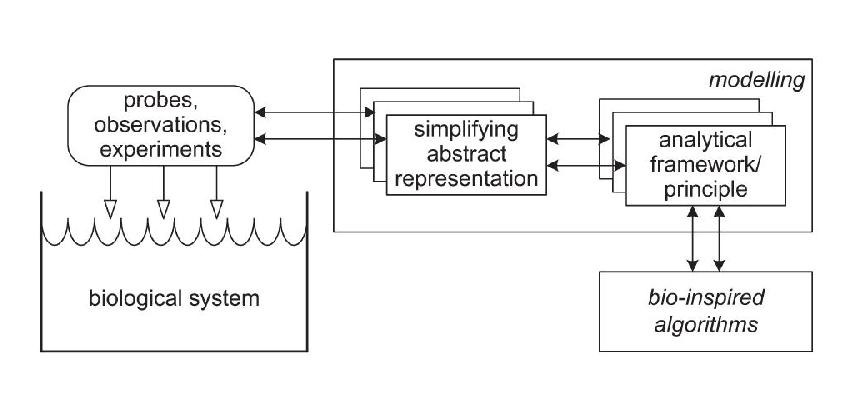
\includegraphics[scale=0.70]{Background/meth-conceptualframework}
	\caption{Depiction of the conceptual framework for devising Biological Inspired Algorithms, taken from \cite{Stepney2005}}
	\label{pic:meth-conceptualframework}
\end{figure}

%
% Immunology as Information Processing
%
\subsubsection{Immunology as Information Processing}
\label{subsec:iip}
Forrest and Hofmeyr summarised their AIS research efforts at the University of New Mexico and the Santa~Fe Institute as ``\emph{immunology as information processing}'' \cite{Forrest2001}. They define information as spatio-temporal patterns that can be abstracted and described independent of the biological system, and information processing as computation with these patterns. They proposed that such patterns are encoded in the proteins and other molecules of the immune system, and that they govern the behaviour of the biological system. They suggest that their information processing perspective can be contrasted with the conventional structural perspective of cellular interactions as mechanical devices. They consider a simple four-step procedure for the investigation of \emph{immunology as information processing}, transitioning from the biological system to a usable computational tool:

\begin{enumerate}
	\item Identify a specific mechanism that appears to be interesting computationally.
	\item Write a computer program that implements or models the mechanism.
	\item Study its properties through simulation and mathematical analysis.
	\item Demonstrate capabilities either by applying the model to a biological question of interest or by showing how it can be used profitably in a computer science setting.
\end{enumerate}

The procedure is similar to the outlined in the conceptual framework for Biologically Inspired Algorithms in that in addition to identifying biological mechanisms (input) and demonstrating a resultant algorithms (output), the procedure (1) highlights the need for abstraction involving modelling the identified mechanism, and (2) highlights the need to analyse the models and abstractions. The procedure of Forrest and Hofmeyr can be used to specialise Stepney, et~al. conceptual framework by clearly specifying the immunological information processing focus.

%
% Experimental Methodology
% Taken from: A Note on Research Methodology and Benchmarking Optimization Algorithms
% 
\subsection{Experimental Methodology}
\label{subsec:methodology:experimental}
% introduce optimization
Optimization is a generalized class of problem involving improvement of a structure under a cost function. It is a one of a few standard perspectives for the investigation and application for computational intelligence systems, specifically including clonal selection algorithms. As such, this section considers the state of optimization algorithm experimental methodology, the concerns of which are applicable to the investigation of computational intelligence algorithms in general.

% into optimization
When it comes to evaluating an optimisation algorithm, every researcher has their own thoughts on the way in which to proceed. Unfortunately, many empirical evaluations of optimisation algorithms are performed and reported without addressing basic experimental design considerations. Perhaps before an experimental methodology can be adopted, a researcher or practitioner may be paralysed by the perceived pessimism of the \emph{no free lunch} theorem that contends the futility of the benchmarking exercise. A pervasive problem in the field of Computational Intelligence algorithms is the lack of meaningful and consistent algorithm experimental and benchmarking methodology. This includes but is not limited to issues of the selection of problem instances, the selection of algorithm specifications, the algorithm configuration parameters, and interpretation of results. The intention of this section is to summarise the general concerns of experimental methodology, with a focus on benchmarking Computational Intelligence algorithms in the face of the `no free lunch' theorem.

%
% No Free Lunch
%
\subsubsection{No Free Lunch}
Wolpert and Macready's \emph{No Free Lunch Theorem} of search and optimisation has caused a lot of pessimism and misunderstanding, particularly in related to the evaluation and comparison of computational intelligence algorithms \cite{Wolpert1997, Wolpert1995}. In simplest terms, the theory indicates that when searching for an extremum of a cost function, \emph{all algorithms perform the same when averaged over all possible cost functions}. The implication is that the often perused general-purpose optimisation algorithm is theoretically impossible. The theory applies to stochastic and deterministic optimisation algorithms, and to algorithms that learn and adjust their search strategy over time. It is invariant to the performance measure used as well as the representation selected. Perhaps the catalyst for benchmarking cynicism is a comment accompanying the proof suggesting that: ``\ldots \emph{comparisons reporting the performance of a particular algorithm with a particular parameter setting on a few sample problems are of limited utility}'' \cite{Wolpert1997}.
% more
The theorem is an important contribution to computer science, although its implications are theoretical. The original paper was produced at a time when grandiose generalisations were being made as to algorithm, representation, or configuration superiority. The practical impact of the theory is to \emph{bound claims of applicability}. Wolpert and Macready encouraged effort be put into devising practical problem classes and the matching of suitable algorithms to problem classes. Further they compelled practitioners to exploit domain knowledge in optimisation algorithm application, now an axiom in the field. 

%
% Issues of Benchmarking Methodology
%
\subsubsection{Issues of Benchmarking Methodology}
Empirically comparing the performance of algorithms on problem instances is a staple for the fields of heuristics and Computational Intelligence, and the problems of effective comparison methodology have been discussed since the inception of these fields. Johnson suggested that the coding of an algorithm is the easy part of the process, that the difficult work is getting meaningful and publishable results \cite{Johnson2002}. He provides a very through list of questions to consider before \emph{racing} algorithms, as well as what he describes as his \emph{pet peeves} within the field of empirical algorithm research. Hooker (among others) condemns what he refers to as \emph{competitive testing} of heuristic algorithms, calling it \emph{fundamentally anti-intellectual} \cite{Hooker1995}. Hooker continues by strongly encouraging a rigorous methodology of what he refers to as \emph{scientific testing} where the aim is to investigate algorithmic behaviours. Barr, et~al. list a number of properties worthy of a heuristic method making a contribution, which can be paraphrased as; efficiency, efficacy, robustness, complexity, impact, generalisability and innovation \cite{Barr1995}. Barr, Golden et~al. specify a loose experimental set-up methodology with the following intuitive steps; 1) define the goals of the experiment, 2) select measure of performance and factors to explore, 3) design and execute the experiment, 4) Analyse the data and draw conclusions, and finally 5) report the experimental results. They then suggest eight guidelines for reporting results, in summary they are; reproducibility, specify all influential factors (for example code and computing environment), be precise regarding measures, specify parameters, use statistical experimental design, compare with other methods, reduce variability of results, ensure results are comprehensive. 

Peer, et~al. summarise the problems of algorithm benchmarking (with a bias toward Particle Swarm Optimisation) to the following points; duplication of effort, insufficient testing, failure to test against state-of-the-art, poor choice of parameters, conflicting results, and invalid statistical inference \cite{Peer2003}. Eiben and Jelasity site four problems with the state of benchmarking evolutionary algorithms; (1) test instances are chosen ad~hoc from the literature, (2) results are provided without regard to research objectives, (3) scope of generalised performance is generally too broad, and (4) results are hard to reproduce \cite{Eiben2002}. 
% overview
The general problems with benchmarking methodology may be distilled into the following sub-problems:

\begin{itemize}
	\item \emph{Parameter Selection}: Computational Intelligence algorithms are typically parameterised, although the mapping of parameter values to predictable effects on problem domains is generally poorly understood. This is because typically unknown and non-linear dependencies commonly exist between the variables resulting in the algorithm being consider a complex system. Francois and Lavergne discuss the deficiencies of the traditional \emph{trial-and-error} and the \emph{experienced-practitioner} approaches to parameter tuning, further suggesting that seeking general rules for parameterisation will lead to optimisation algorithms that offer neither convergent or efficient behaviours \cite{Francois2001}. There are many solutions not limited to the following: consulting the literature although often ignored \cite{Eiben2002}), generalise from large numbers of experiments \cite{Schaffer1989}, self-adaptive parameters, meta-algorithms for searching for good parameters values, and statistical sensitivity analysis over parameter ranges \cite{Chan1997, Birattari2002}. 
	
	\item \emph{Problem Selection}: Problem instances should be selected to demonstrate specific behaviours of the systems under study. Typically benchmarks are performed on ad~hoc lists of standard benchmark instances, that although offering the benefit of comparability, typically devolve into racing contest. Eiben and Jelasity support the division of problem instances into categories and encourage the evaluation of optimisation algorithm over a large number of test instances \cite{Eiben2002}. In their paper on understanding the interactions of Genetic Algorithm parameters Deb and Agrawal propose four structural properties of problems for testing genetic algorithms; multi-modality, deception, isolation, and collateral noise \cite{Deb1999}. Yao, et~al.  divide their large test dataset into the categories of uni-modal, multi-modal with many local optima, and multi-modal with few local optima \cite{Yao1999}. Whitley, et~al.  provide a detailed study on the problems of selecting test instances for genetic algorithms, and suggest that difficult problem instances should be non-linear, non-separable, and non-symmetric \cite{Whitley1996}.
	
	\item \emph{Measure Selection}: There are many ways to measure the performance of an algorithm for a problem instance, although the most common involves measures of \emph{efficacy} (problem specific costs) and \emph{efficiency} (computation space and/or time). Most Biologically Inspired Algorithms have a stochastic element, typically in their random starting position(s) and in the probabilistic decisions made during sampling of the domain. Therefore, the measuring of performance must be repeated a number of times to account for the stochastic variance\footnote{Typically $\geq30$ according to the central limit theorem such that the underlying distribution can be meaningfully summarised.}, which also could be a measure of comparison between algorithms. The most critical concern in the selection of measures is that of standardisation for the purposes of comparison \cite{Birattari2005a, Barr1995}.	
	
	\item \emph{Statistical Significance}: The scientific knowledge of Computational Intelligence is predominantly accrued as empirical observations and conclusions. Therefore, there is a need for methods that permit interpretation and conclusions to be drawn beyond the standard reporting of results. Statistical hypothesis testing and related methods provides such tools, although unfortunately are rarely employed. Peer, et~al. \cite{Peer2003} and Birattari and Dorigo \cite{Birattari2005} provide a basic introduction (suitable for an algorithm-practitioner) into the appropriateness of various statistical tests for algorithm comparisons. Parametric statistical methods are used for interval and ratio data (like a real-valued performance measure), and non-parametric methods are used for ordinal, categorical and rank-based data. Interval data is typically converted to ordinal data when salient constraints of desired parametric tests (such as assumed normality of distribution) are broken such that the less powerful non-parametric tests can be used. The use of non-parametric statistical tests maybe preferred as some authors (for example \cite{Chiarandini2005}) claim the distribution of cost values are very asymmetric and/or not Normal.
\end{itemize}

%
% Integrated Methodology
% Taken from 'Small Models': A Methodology for Designing and Investigating Adaptive Systems
%
% Omitted the genetic algorithm Section~(ga, innovation)
% 
\subsection{Designing and Investigating Adaptive Systems}
\label{subsec:smallmodels}
Complex and adaptive systems are difficult to design and investigate, therefore the need for a coherent and proven methodology for such activities is paramount. Inspired by an interpretation of the achievements of the Wright brothers in achieving the first powered flight, this section provides a summary of a methodology for investigating and designing \emph{conceptual machines} proposed by David Goldberg \cite{Goldberg2002}. 

For the purposes of clarity, a \emph{model} is a conceptualisation that provides a description of a system that accounts for its properties and may be used to study the characteristics of the system. For the remainder of this thesis, conceptual models are instantiated as \emph{algorithms} for the purposes of computational implementation, simulation, and study. The algorithms provide procedures for problem-solving when the behaviour of the instantiated model suitably match the characteristics of a problem.

%
% Engineers and Mathematicians
%
\subsubsection{Engineers and Mathematicians}
Goldberg describes the airplane and other products of engineering as \emph{material machines}, and distinguishes them from the engineering of genetic algorithms and other adaptive systems as \emph{conceptual machines}. He argues the methodological distinction between the two is counter-productive and harmful from the perspective of conceptual machines, specifically that the methodology of the material is equally applicable to that of the conceptual \cite{Goldberg1999a}. The obsession of mathematical rigour in computer science, although extremely valuable, is not effective in the investigation of adaptive systems given their complexity. Goldberg sights the airplane as an example where the engineering invention is used and trusted without a formal proof that the invention works (that an airplane can fly\footnote{Goldberg is quick to point out that sets of equations do exist for various aspects of flight, although no integrated mathematical proof for airplane flight exists.}). This defence leads to what Goldberg refers to the \emph{economy of design} which is demonstrated with a trade-off that distinguishes `model description' (mathematician-scientists) that is concerned with model fidelity, and model prescription (engineer-inventor) that is concerned with a working product. In descriptive modelling \emph{the model is the thing} (of interest) whereas in `prescriptive modelling', \emph{the object is the thing} (of interest). In the latter, the model (and thus its utility) serves the object, in the former model accuracy may be of primary concern. This economy of modelling provides a perspective that distinguishes the needs of the prescriptive and descriptive fields of investigation. 

The mathematician-scientist is interested in increasing model accuracy at the expense of the speed (slow), where as the engineer may require a marginally predictive (inaccurate) model relatively quickly. This trade-off between high-cost high-accuracy models and low-cost low-fidelity models is what may be referred to as the \emph{modelling spectrum} that assists in selecting an appropriate level of modelling. Goldberg proposes that the field of genetic algorithms expend too much effort at either ends of this spectrum. There is much work where there is an obsession with blind-prototyping many different tweaks in the hope of striking it lucky with the \emph{right} mechanism, operator, or parameter. Alternatively, there is also an obsession with detailed mathematical models such as full-blown differential equations and Markov chains. The middle ground of the spectrum, what Goldberg refers to as \emph{little models} is a valuable economic modelling consideration for the investigation of conceptual machines to \emph{do good science through good engineering}. 

%
% Methodology
%
\subsubsection{Methodology}
The methodology has been referred to as post-modern systems engineering and is referred to by Goldberg as a methodology of innovation \cite{Goldberg2004}. The core principles of the process are as follows: 

\begin{enumerate}
	\item \emph{Decomposition}: Decompose the large problem approximately and intuitively, breaking into quasi-separate sub-problems.
	\item \emph{Modelling}: Investigate each sub problem separately (or as separate as possible) using empirical testing coupled with adequately predictive, low-cost models.
	\item \emph{Integration}: Assemble the sub-solutions and test the overall invention, paying attention to unforeseen interactions between the sub-problems.
\end{enumerate}

%
% Decomposition
%
\paragraph{Decomposition} Problem decomposition and decomposition design is an axiom of reductionism and is at the very heart of problem solving in computer science. Therefore, it is not worth dwelling on the topic other than to comment as to its meaning within the context of adaptive systems. One may consider the base or medium on which the system is performing its computation mechanisms, the so-called building blocks of information processing. A structural decomposition may involve the architecture and data structures of the system. Additionally, one may also consider a functional breakdown of mechanisms such as the operators applied at each discrete step of an algorithmic process or mechanisms. The reductions achieved provide the basis of investigation and modelling.

%
% Small Models
%
\paragraph{Small Models} Given the principle of the economy of modelling presented as a spectrum, one may extend the description of each of the five presented model types. \emph{Small Models} refers to the middle of the spectrum, specifically to the application of dimensional and facet-wise models. These are mid-range quantitative models that make accurate prediction over a limited range of states at moderate cost. Once derived, this class of models generally requires a small amount of formal manipulation and large amounts of data for calibration and verification. The following summarises the modelling spectrum:

\begin{itemize}
	\item \emph{Unarticulated Wisdom}: (low-cost, high-error) Intuition, what is used when there is nothing else.
	\item \emph{Articulated Qualitative Models}: Descriptions of mechanisms, graphical representations of processes and/or relationships, empirical observation or statistical data collection and analysis.
	\item \emph{Dimensional Models}: Investigate dimensionless parameters of the system.
	\item \emph{Facet-wise Models}: Investigation of a decomposition element of a model in relative isolation.
	\item \emph{Equations of Motion}: (high-cost, low-error) Differential equations and Markov chains.
\end{itemize}

Facet-wise models are an exercise in simple mathematics that may be used to investigate a decomposition element of a model in relative isolation. They are based on the idea of \emph{bracketing high-order phenomena} by simplifying or making assumptions about the state of the system. An example used by Goldberg from fluid mechanics is a series of equations that simplify the model by assuming that a fluid or gas has no viscosity, which matches no known substance. A common criticism of this modelling approach is ``\emph{system X doesn't work like that, the model is unrealistic}''. The source of such concerns with adaptive systems is that their interactions are typically high-dimensional and non-linear. Goldberg's response is that for a given poorly understood area of research, any useful model is better than no model. Dimensional analysis or the so-called dimensional reasoning and scaling laws are another common conceptual tool in engineering and the sciences. Such models may be used to investigate dimensionless parameters of the system, which may be considered the formalisation of the systemic behaviours.

%
% Integration
%
\paragraph{Integration} Integration is a unification process of combining the findings of various models together to form a \emph{patch-quilt} coherent theory of the system. Integration obviously is not limited to holistic unification, one may address specific hypothesis regarding the system resulting in conclusions about existing systems, and design decisions pertaining to the next generation of systems.

%
% Application
%
\paragraph{Application} In addition to elucidating the methodology, Goldberg specifies a series of five useful heuristics for the application of the methodology as follows (taken from \cite{Goldberg1999a}, page 8):

\begin{enumerate}
	\item \emph{Keep the goal of a working conceptual machine in mind}. Experiments commonly get side tracked by experimental design and statistical verification; theoreticians get side tracked with notions of mathematical rigour and model fidelity.
	\item \emph{Decompose the design ruthlessly}. One cannot address the analytical analysis of a system like a genetic algorithm in one big `gulp'.
	\item \emph{Use facet-wise models with almost reckless abandon}. One should build easy models that can be solved by bracketing everything that gets in the way.
	\item \emph{Integrate facet-wise models using dimensional arguments}. One can combine many small models together in a patch-quilt manner and defend the results of such models using dimensional analysis.
	\item \emph{Build high-order models when small models become inadequate}. Add complexity to models as complexity is needed (economy of modelling).
\end{enumerate}

%
% Summary
% Provides an overview of the chapter and its structure, and a description of what is intended to be achieved by providing this documentation. A description of why and how this chapter follows on from the previous chapter
%
\section{Chapter Summary}
\label{sec:background:summary}
% broad position
This Chapter positioned the investigation broadly in the field of Biologically Inspired Computational Intelligence, a sub-field of Artificial Intelligence, and specifically in the field of Artificial Immune Systems. 
% motivation - clonal selection
Clonal Selection was highlighted as an adaptive paradigm in the field of Artificial Immune Systems that underlies much of the general field.
% motivation - distributed
Distributed Artificial Immune Systems including distributed Clonal Selection Algorithms is an over promised and under delivered, although potentially beneficial field of study. An effective realisation of distributed clonal selection algorithms is expected to facilitate the broader application of such approaches to classes of problem that may benefit from parallel and cooperative problem solving strategies, such as problems with functional or information availability decompositions.
% motivation - using biology
Turning back to the structure and function of the immune system to develop new AIS approaches including distributed approaches is currently an advocated approach in the field given the apparent impasse experienced in the progress of such approaches. 
% methodology
A systematic framework was adopted for the development of new immunologically inspired approaches, with careful empirical investigation, and awareness of the economy of models and need for the re-integration of findings.
% next
This chapter both positioned and motivated the research hypothesis outlined in Chapter \ref{chap:introduction}, and defined the systematic methodology adopted for the development and investigation of adaptive and distributed clonal selection algorithms throughout the remainder of the dissertation. Toward this end, Chapter \ref{chap:cs} provides an in depth investigation into the clonal selection paradigm, both reviewing and elaborating the cellular perspective of such approaches which is later pursued in Chapter \ref{chap:cells}, and outlining the agenda for realising distributed approaches in Chapters \ref{chap:tissues} and \ref{chap:hosts}.

% EOF
	%
% Clonal Selection Paradigm Chapter
% Jason Brownlee
%

\chapter{Clonal Selection Paradigm}
\label{chap:cs}

%
% Overview
% Provides an overview of the chapter and its structure, and a description of what is intended to be achieved by providing this documentation. A description of why and how this chapter follows on from the previous chapter
%
\section{Chapter Overview}
\label{sec:cs:overview}
% general
This chapter provides an in depth review of clonal selection theory and inspired computational algorithms, highlighting the open problems in the state of the field that specifically motivate the work.
% theory
Section~\ref{sec:cs:theory} reviews the clonal selection theory and relevant immunochemistry and theoretical immunology providing a detailed foundation to effectively interpret the motivations for the state of clonal selection algorithm research. 
% algorithms
The field of clonal selection algorithms is reviewed in Section~\ref{sec:cs:algorithms} providing a compressive taxonomy of approaches and focusing on the abstracted immunological principles and application domains for resultant systems. The review identifies three limitations that motivate the remainder of the chapter, specifically (1) the lack of placement of clonal selection approaches in a broader context, (2) the lack of explicit investigation of clonal selection as an adaptive system, and (3) the cellular focus of abstracted computational principles.
% limitations
These general open problems are investigated in turn. Section~\ref{sec:cs:related} reinforces the relationship of the paradigm with evolutionary algorithms and instance based learning, and highlights the relationships with binary hill climbing and competitive learning paradigms. Section~\ref{sec:cs:adaptive} investigates clonal selection in the context of adaptive systems theory, highlighting the need to focus on the system-environment relationship of the paradigm, and the general short-sightedness of selection-based adaptive systems. Finally, Section~\ref{sec:cs:beyond} outlines an agenda for investigating the clonal selection paradigm for the remainder of the dissertation, firstly at the classical adaptive cellular level, as well as the inherently distributed `host of tissues' and `population of hosts' perspectives of immunology.

%
% Clonal Selection Theory
%
\section{Clonal Selection Theory}
\label{sec:cs:theory}

%
% Theory of Acquired Immunity
%
\subsection{Theory of Acquired Immunity}
\label{subsec:cs:theory:acquiredimmunity}
This section provides an overview of the theory including its inception, main processes, and the mechanisms employed for diversity. This discussion of clonal selection is limited to the discussion of B-lymphocytes and humoral immunity given that the development and much of the experimental and theoretical work on clonal selection has been completed in this context.

%
% Theory Development
%
\subsubsection{Theory Development}
\label{subsubsec:theory:development}
Paul Ehrlich observed the exponential generation of antibodies triggered by the primary exposure to antigen in blood. He proposed a \emph{side-chain theory} (circa 1900) in which blood cells naturally made side chains (now known as receptors) capable of binding to all antigens. His theory proposed that the information and capability to detect all antigen was already possessed by the host (for example in the genome) and expressed by the antibodies. This model was ultimately rejected because it was demonstrated that antibodies could be produced in response to synthetic substances of which the antibodies could have no prior knowledge. Further, the theory could not explain the improvement in the specificity of the response in the secondary and subsequent exposures to the same antigen. The \emph{antigen-template theory} was proposed and suggested that antigen direct the response \cite{Pauling1940}. In the theory antibodies use the antigen as a template or model and modify themselves to provide a more effective complement. The emerging field of genetics suggested the invalidity of this theory as the specificity of an antibody could not be changed after its creation given that the process of \emph{gene} to \emph{amino acids} to \emph{protein conformation} is one-way. Niles Jerne had great difficulty with the template theory and listing a number of observations to which the theory could not account \cite{Jerne1955}. The template theory proposed a one-to-one relationship between antibodies and antigen, although experimental observations suggested that far more antibodies were produced in the primary response than there were antigen. Further, the template theory suggested the role of antibodies ended after neutralising the antigen, whereas observations indicated that antibodies have a short lifespan, therefore failing to account for observed immunological memory exhibited in the improved specificity of the secondary response. 

Jerne proposed an alternative called the \emph{natural selection hypotheses} of antibody diversity. His theory proposed that the host contains a small pre-existing collection of randomly generated antibodies. In generating this pre-existing pool, self-antibodies where proposed to be \emph{somehow} neutralised before causing harm to the host. The theory proposed that antigen \emph{naturally select} antibodies of high affinity (a good match) from which more antibodies of the same affinity are produced. The result of the antigen-to-antibody selection mechanism the production of antibodies specific to the antigen in large numbers, which presented an improved response of the host to the antigen. Finally, he suggested that copying errors during the triggered production of antibodies may result in an improved fit with the antigen and account for the observed immunological memory effect. In his work on antibodies and allergy, David Talmage extended upon the natural selection hypothesis suggesting that Jerne's theory was an extension of Ehrlich's \emph{side-chain theory}, and that replicating cells, not antibodies, were the main feature of the immune response  \cite{Talmage1957}. Talmage suggested the notion that immune cells must specialise in producing antibodies with the same specificity as the receptors of the surface of the cell that trigger its proliferation. 

Frank Macfarlane Burnet also extended Jerne's theory at the same time as Talmage (and subsequently received priority) focusing on a \emph{clone} perspective and the self-replicating cellular mechanisms during the immune response \cite{Burnet1957}. He called his theory the \emph{clonal selection hypothesis of antibody diversity}. The `missing link' for Burnet was the pre-existing \naive\ antibody population that was proposed in Jerne's theory. As with Talmage's theory, antigen select the best matching cells, that results in their subsequent replication. He suggested that for the selectionist theory to hold, that each cell must produce antibody of one type (all with the same receptor configuration). His theory attributed the exponential rise in the number of antibodies after infection to the exponential rise in the number of antibody producing cells due to clonal expansion of selected cells. It also explained the improved secondary response given the specialisation of receptors during expansion, although the mechanisms by which receptors specialised was only speculated. The following provides a summary of the characteristics of Burnet's clonal selection, from \cite{Burnet1978}:

\begin{enumerate}
	\item \emph{Initial Repertoire}: Randomly generated initial population of antibody producing immune cells.
	\item \emph{One-to-one}: An immune cell can detect and release antibody of one specificity, which is passed on to descendent cells.
	\item \emph{Elimination}: Those initial cells that are reactive to self-tissues are selected against (killed).
	\item \emph{Proliferation}: Generation of antibody and the proliferators of the cell after contact (selection) with antigen.
	\item \emph{Forbidden}: The elimination of progeny that can select for self tissues.
\end{enumerate}

Talmage and Burnet both followed up two years later with monographs elaborating on the theory, providing a more detailed account of the clonal selection process \cite{Talmage1959, Burnet1959}. Burnet continued his work on the study of immunological tolerance, to which his theory supported, and with Peter Medawar won the Nobel Prize in 1960 for work that provided the foundation for viable tissue and organ transplant. It is also interesting to note that it was Burnet who conceptualised the \emph{self-nonself} abstraction of the immune system in his work on immunological tolerance, which like his clonal selection theory has remained a foundational concept of modern immunology\footnote{For an overview of the history of self-nonself paradigm see Crist \cite{Crist2000}}. Nossal and Lederberg supported the one-cell-one-antibody assertion of clonal selection providing first test and confirmatory evidence for the theory \cite{Nossal1958}. As mentioned, Burnet speculated as to the mechanisms for antibody diversification and specialisation in his theory. His prediction of the existence of such a mechanism was confirmed approximately 20 years later by Tonegawa et~al. who investigated the fine tuning of antibody receptors called \emph{somatic hypermutation} for which he later won the Nobel Prize \cite{Hozumi1976, Tonegawa1988}.

%
% Theory Detail
%
\subsubsection{Theory Detail}
\label{subsubsec:theory:summary}
An antigen is a molecule which can elicit an immune response, an antibody (immunoglobulin) is a molecule which can bind to and neutralise an antigen, and a B-lymphocyte is an immune cell which can bind to antigen as well as produce antibodies. The physical surface of an antigen has a number of different structural features called antigenic determinants. An antibody and B-cell have receptors which have a specificity (ability to bind) to only one surface feature of an antigen, although the feature an antibody binds to may be represented on more than one different antigen. A host possesses a base pool of randomly generated  lymphocytes that define the hosts natural immunity, and are prepared during the embryonic stage of development. During this time, the immune system learns a tolerance for the tissues of the host organism and those lymphocytes that are self-reactive are removed from the pool. The repertoire of natural lymphocytes possesses the ability to bind to any antigenic stimulus (natural or synthetic) with some general affinity. The introduction of an antigen triggers an immune response. The lymphocytes that are most suited (have the best complementary shape) for the antigen bind to it triggering cell division and differentiation. Therefore, it is the features of the antigen that select the best matching lymphocytes from the hosts cellular repertoire. After a lymphocyte binds to an antigen it moves to lymphatic tissue (germinal centre) to begin the differentiation process. The function of this process is the preferential proliferation to replicate a clone of cells to produce antibody capable of neutralising the triggering antigen. The lymphocyte proliferates and differentiates into two different cell types: \emph{plasma cells} that continue to replicate and which release large numbers of antibody, and \emph{memory cells} that like the parent cell act as a catalyst for response to subsequent infections. 

During the proliferation and differentiation process copying errors (somatic mutations) may occur with a probability of mutation much higher than the genetic mutations that occur in typical cell divisions. The result is a clone of lymphocytes that have receptors similar to the parent cell, although vary slightly in their specificity to the triggering antigen. This means that on subsequent exposures to the antigen, the host possesses a larger repertoire of lymphocytes and antibodies capable of neutralising the antigen. Given the somatic mutations introduced during replication, some of the lymphocytes will contain an improved match for the antigen, improving their chance of being selected. An antibody producing lymphocyte will only produce antibodies of the same affinity. This means that after the cell has formed (after mitosis) it may be considered an antibody factory where all antibodies produced have the exact same complementary shape for a specific antigen surface feature. The fact that a surface feature may be represented by more than one antigen provides the basis for vaccinations. This commonality of shape facilitates the capability for generalisation, where lymphocytes and antibody may be raised on one harmless antigen and be effective on other more harmful antigens that possess the same structures. The memory cells generated during the differentiation process may live for months and years which is much longer than typical lymphocytes that lives for hours or days, providing long term memory of the learned antigenic defence.

The problem of antibody diversity was considered for at least 100 years before a coherent theory was proposed, although it is important to highlight that the theory in its original inception was not perfect. Specific details, such as the mechanisms of diversity where not known for many years after the theory's acceptance. Silverstein suggested that with regard to the clonal selection theory, like Darwin's theory of evolution by \emph{natural} selection, much of the specifics have been out-dated given scientific progress \cite{Silverstein2002}. Rather than abandon the core principles, Silverstein emphasises the need to embrace the continually updated version of the theory. A pioneer himself in immunology, Lederberg suggests similar sentiments: ``\emph{Don't let conflicting and awkward `facts' stand in the way of an esthetically satisfying theory whose fundamentals are consistent with the world model and with one another! And be suspicious of `facts' that seem in the way of any coherent theory}'' \cite{Lederberg1988} (page 181).

Finally, the clonal selection process of acquired immunity is not without problems. An observed effect known as \emph{Original Antigenic Sin}\footnote{``Original Sin'' is a term from Christian theology describing the condition of sin that marks all humans as a result of Adam's first act of disobedience.} refers to the commitment of the immune response and subsequent memory to specific surface characteristics of a pathogen, such as a virus, then having the virus mutate and change those surface characteristics \cite{Francis1960, St.Groth1966}. The result of the commitment is that the previously high-affinity lymphocytes and antibody become low-affinity within the context of the change to the virus. Given the clonal selection and expansion of lymphocytes in the first exposure, the now low affinity receptors dominate the subsequent exposures, effectively out-competing other lymphocytes that may be better suited to the changed virus.

%
% Diversity Mechanisms
%
\subsubsection{Diversity Mechanisms}
\label{subsubsec:theory:diversity}
The genetics and chemistry of antibody diversity is beyond the scope of this work. This section provides a summary of the main mechanisms that lead to the diversity of the B-lymphocyte repertoire, which includes gene recombinations, somatic mutations, receptor editing, class switching, and gene conversion.

\begin{itemize}
	\item \emph{Genetic Recombination}: The process that accounts for the initial and on-going high diversity of new lymphocytes is called \emph{secondary V(D)J rearrangements}, which refers to the recombination of the genetic code during the development of B-lymphocytes. This genetic recombination process accounts for the diversity of the initial lymphocyte repertoire and in the creation of new (known as \naive) B-lymphocytes \cite{Tonegawa1983, Tonegawa1988}.
	
	\item \emph{Somatic Hypermutation}: Along with genetic recombination was the first discovery made regarding the genetic component of antibody diversity \cite{Tonegawa1983}. It refers to the point mutations of the genome that occur during the clonal expansion phase when the cell moves to the germinal centre for differentiation (for more information regarding cell maturation see \cite{Berek1991, Berek1993}). The mutations are targeted at the genes in the genome that code for the receptors and occur at a rate about one million times higher than the mutation rates in other genes. Mutations include substitutions, additions, and deletions of genetic code. Specific sequences (motifs) within the receptor genes are targeted with high frequency, referred to as `hot spots'.
	
	\item \emph{Receptor Editing}: Clonal selection proposes that those cells with receptors that bind to self-tissues (auto-reactive) are clonally deleted before they can cause damage. Receptor editing is an additional process for re-programming auto-reactive receptors by recombining their genes \cite{Rajewsky1998, Nussenzweig1998}. Those cells that have receptors that are still auto-reactive after this \emph{editing} process are eliminated from the repertoire. Receptor editing was proposed to occur before somatic mutation and in response to contact with antigen (similar to template theory). It has also been proposed that receptor editing may provide an additional general receptor diversity mechanism for so-called `long jumps' (large changes) in receptor affinity \cite{George1999}.
	
	\item \emph{Class Switch Recombination}: The genetic recombination that results in antibodies changing their behaviour by \emph{becoming} different immunoglobulin types, although maintaining the same specificity for antigen \cite{Harriman1993, Li2004}. Gene conversion is another genetic recombination process and the primary mechanism for diversification of immune receptors in chickens (and some other species) that is employed instead of somatic mutation used in mammals \cite{Wysocki1989, Li2004}.
\end{itemize}

%
% Shape Space and Affinity Landscape
%
\subsection{Shape Space and Affinity Landscape}
\label{subsec:cs:ssandal}
The \emph{shape-space} formalism and its sibling the \emph{affinity landscape} are two common geometric paradigms from theoretical immunology, both of which have had a recent revival and reapplication in the related field of Artificial Immune Systems. This section briefly surveys the history of these terms in the context of computational immunology, and consider their pervasive application in AIS. 

%
% Shape-Space
%
\subsubsection{Shape-Space}
Perelson and Oster introduced the shape space formalism in their theoretical investigation of antibody repertoire size and reliable recognition \cite{Perelson1979}. Given antibody $ab$ and antigen $ag$, the authors discretised the physical aspects of the antibodies combining site and the antigenic determinant into a vector of $n$ so called \emph{shape} parameters. The parameters included the set of intermolecular forces important to the $ab-ag$ recognition. The abstraction of a molecule was later referred to as its \emph{generalised shape}, where the shape parameters for a $ag$ and $ab$ molecule may be defined as points in an $n$-dimensional Euclidean space called \emph{shape-space} $S$ \cite{Perelson1989}. The authors suggested that given an adequate method of defining molecule shape, the dimensionality of such a space could be relatively small (as low as five dimensions). Further, the formalism simplified the complementarity nature of $ab-ag$ interactions, thus rather than the matching convention of $ab \neq ag$, the formalism considers $ab=ag$. Given this simplification, the formalism defines distances between $ab$ and $ag$ in the Euclidean shape space as the \emph{degree of complementarity} or \emph{affinity} of the interaction. A generalised affinity function may be defined as $c_{ij}=f(x_{i},x_{j})$, where $c_{ij}$ is the affinity between the molecules $i$ and $j$, and $x_{i}$ and $x_{j}$ are vectors representing the molecules in shape space, $f$ is an appropriate function for the selected representation. The shape space is defined as a finite hypercube, with a volume $V$ of uniform density. Each antibody was defined with a local recognition region in the shape space $\epsilon$, with a Gaussian falloff. An $ab$-$ag$ interaction only occurs if the $ag$ is above an affinity threshold, within the triggering hyper-sphere of the $ab$. In their application of the model, random distributions of $ab$ and $ag$ were used and self-antigens were ignored.

\begin{figure}[ht]
	\centering
	\fbox{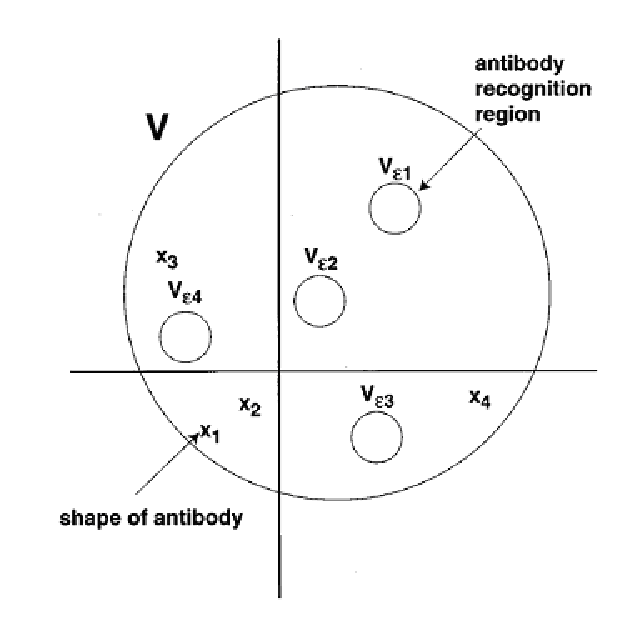
\includegraphics[scale=0.65]{ClonalSelection/theory-shapespace}}
	\caption{Depiction of the shape-space formalism taken from \cite{Perelson1997} (page 1225). $X_{i}$ represents antibodies with corresponding complementary recognition volumes $V_{\epsilon i}$.}
	\label{pic:theory:shapespace}
\end{figure}

%others
The shape-space formalism provides a geometric way to consider molecule interactions in the context of the immune system, it was not the first of such a geometric abstraction of molecular interaction. For example, Write considered a \emph{genotypic-space} for possible gene combinations and a mapping onto the now ubiquitous \emph{fitness landscape} in theoretical genetics \cite{Wright1932}. 
% usage
This fundamental $ag-ab$ interaction paradigm was used throughout the late 1980's and 1990's predominantly in theoretical works modelling clonal selection and various aspects of Jerne's idiotypic network theory (for example work on a one-dimensional Euclidean shape-space by Segel \cite{Segel1988}, and an investigating the stability of the idiotypic model by Perelson \cite{Perelson1989}). Carneiro and Stewart criticised the shape-space formalism, focusing on the simplicity of the abstracted space and the shortcomings of the simple affinity functions \cite{Carneiro1994}. They cautioned against the extrapolation of results from the abstraction to the real shape-space, highlighting that the dimensionality of the space should be much higher (at least 10, and as high as 20), and that the affinity mapping function would have to be irregular and discontinuous. They support their claims with observations from simulated docking of molecules based on crystallographic structures. They propose a splitting of the formalism into a \emph{realistic shape-space} in which real molecules can be evaluated, and an abstracted \emph{inversion space} as a tool for modelling.

%
% Affinity Landscape
%
\subsubsection{Affinity Landscape}
\label{subsubsec:cs:theory:affinitylandscape}
It is typical in physics for systems to minimise some utility in the context of a response surface, whereas in biology it is common for systems to maximise some utility. This is highlighted by the already mentioned evolutionary fitness landscape paradigm introduced by Wright in conceptualising gene combinations \cite{Wright1932}. In the immune system, one may consider the utility of an antibody as its affinity in binding to a specific antigen. A related concern called \emph{avidity}, refers to strength of the binding between antigen and antibody. Among the first to employ the conceptualisation of an \emph{affinity landscape} were Kauffman and Weinberger who used this geometric paradigm in the field of theoretical immunology to investigate and describe the theoretical effects of affinity maturation \cite{Kauffman1989, Kauffman1988}. They investigated adaptive walks using Kauffman's NK\footnote{Not to be confused with Natural Killer cells, $N$ and $K$ are parameters of the Kauffman's model.} model on the affinity landscape based on antibody sequences or so called \emph{antibody-space} in response to a given antigen. Kauffman and others used the NK model to investigate various molecular sequence spaces and the corresponding response surfaces, for example \cite{Farmer1986, Kauffman1993, Kauffman1987}. One may define an affinity landscape as a degree of complementarity response surface for a given collection of antigen detecting agents (lymphocytes and antibody), for a given \emph{specific} antigenic determinant. Abstractions of this surface considered in theoretical immunological are typically continuous, the topology of which consists of many local optima. Detecting agents may navigate this response surface through the process of affinity maturation, which involves manipulations to genotypic sequence information (such as the clonal selection diversity mechanisms discussed in Section~\ref{subsubsec:theory:diversity}).

The affinity landscape is a simple yet important conception, and although Kauffman et~al. were perhaps the first to apply such a name, the geometric formalism was no doubt in the mind of Perelson and others in the early days of theoretical and computational immunology. The formalism has played an important role in conceptualising and formalising \emph{affinity maturation} of the immune response by hypermutation (for example see \cite{Pierre1997, Shannon1999, Theodosopoulos2004, Theodosopoulos2005}), which as has been demonstrated is a critical aspect of the clonal selection theory of antibody diversity. George and Gray used the affinity landscape as a crutch in describing their theories on receptor editing, which were generalised very effectively on a simple two-dimensional affinity graph in Figure~\ref{pic:theory:affinitylandscape} \cite{George1999, George2000}.

\begin{figure}[ht]
	\centering
	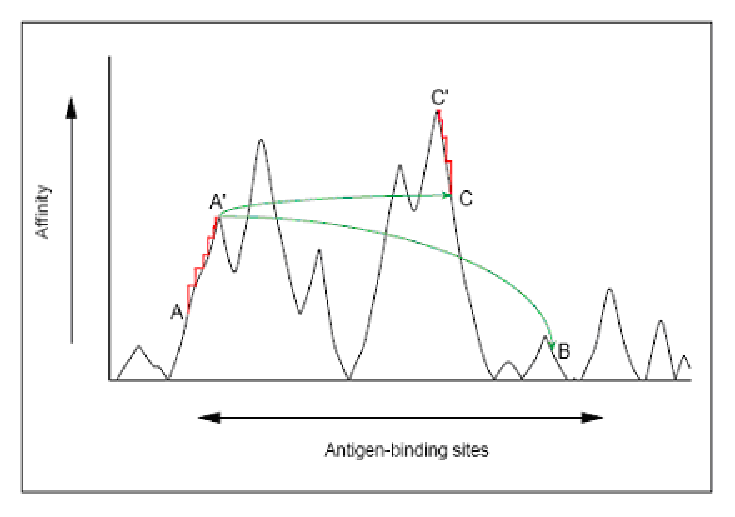
\includegraphics[scale=0.65]{ClonalSelection/theory-affinitylandscape}
	\caption{Theory of receptor editing providing long jumps in the affinity landscape, from \cite{George1999}.}
	\label{pic:theory:affinitylandscape}
\end{figure}

%
% Artificial Immune Systems
%
\subsubsection{Artificial Immune Systems}
\label{subsubsec:cs:theory:ais}
The shape-space and affinity landscape paradigms have been widely used in the field of Artificial Immune Systems. Some examples include the quintessential binary shape-space used in negative selection (for example \cite{Stibor2005}) and immune network algorithms, the recognition region and threshold used in data mining and classification algorithms \cite{Watkins2001, Watkins2004a, Knight2005}, and the affinity landscape cost functions navigated by optimisation algorithms \cite{White2003, Castro2002}. The usage of these paradigms is unified in the framework for AIS of Engineering de~Castro and Timmis, and listed in Section~\ref{subsec:background:problems:review}. The authors presented abstract models of immune cells, molecules and their interactions including the affinity landscape and shape-space paradigms in an effort to elaborate the three facets of their framework (representation, affinity measures, and immune algorithms). One may distil the discussion of the AIS Engineering Framework and related abstraction by de~Castro and Timmis, to a triad relationship between \emph{representation} in a shape-space, a \emph{mapping} function between points in that space, and an \emph{affinity landscape} of scores assigned by the mapping function, as follows:

\begin{itemize}
	\item \emph{Representation}: Extending the shape-space paradigm, the sequence, or search space is considered essentially a representation domain. Examples provided include real-valued, binary, integer and symbolic. 	
	\item \emph{Mapping}: A function that translates from the representation shape-space to an affinity landscape surface. Distance and matching within the shape-space are the mapping functions discussed with a number of appropriate suggestions for the various shape-spaces listed. A point in one of these spaces may have a \emph{recognition region}, and a \emph{cross-reactive threshold}. A mapping function may be complemented with an additional threshold binding function, perhaps to convert a scalar affinity into a decision variable.	
	\item \emph{Affinity}: Affinity may be further abstracted from the degree of complementarity in an antibody-antigen interaction, to a more general scoring assigned to the mapping between points in the shape-space. Affinity may be a measure of quality of an agent in a specific environment or in the context of a specific requirement.
\end{itemize}

The proposed triad provides a geometric interpretation and relation of \emph{shape-space} to \emph{affinity landscape} paradigms and provides an open framework for investigating immunological principles in domains, not limited to the pattern recognition problem. One may consider further geometric conceptions related to affinity maturation in immune system that lack a suitable formalism, let alone an abstraction for use in Artificial Immune Systems. Two examples may include: (1) the aggregation of multiple affinity landscapes, that is the affinity of a repertoire in the context of an antigenic environment not limited to one antigen, and (2) the temporal and spatial aspects to affinity throughout the host organism in the context of lymphocyte and antibody mobility.


%
% Clonal Selection Algorithms
%
\section{Clonal Selection Algorithms}
\label{sec:cs:algorithms}
The previous section outlined in detail the abstraction, immunochemistry, and theoretical immunology that inspired the field of clonal selection algorithms. The review highlighted that the main actors in clonal selection are cells, antibodies, and antigen, and the main processes are selection, proliferation, and genetic mutations. Further, it showed that the common measures used to describe the relationship between antibody and antigen are affinity and avidity, and that the main conceptual formalisms used to describe the constraints and effects of such interactions are shape-space and the affinity landscape. This section reviews the so called \emph{clonal selection principle} which is the abstraction that motivates the field of clonal selection algorithms. A taxonomy of such algorithms is presented, highlighting the open problems in the state of the art.

%
% From Theory to Principle
%
\subsection{From Theory to Principle}
\label{subsec:cs:algorithms:principle}
% de~Castro and Timmis
In the glossary of their seminal book on Artificial Immune Systems, de~Castro and Timmis provided a definition of the clonal `selection principle' as ``\emph{the prevalent theory stating that the specificity and diversity of an immune response are the result of selection by antigen of specifically reactive clones from a large repertoire of preformed lymphocytes, each with individual specificities}'', not distinguishing between the theory and information processing abstraction \cite{Castro2002a} (page 322). In their treatment of Burnet's theory, the authors comment that lymphocytes may be considered to undergo a process similar to natural selection and that only those cells that contact an antigen may be selected for proliferation, strongly highlighting the Darwinian connection made by Jerne and Burnet. The authors focused on the clonal expansion and variation aspects of the process, referring to the abstraction of the theory as \textbf{affinity maturation of the immune response}. They propose two important computational features of the theory in their abstraction (page 80): (1) An antigen selects multiple cells to proliferate where each cell has an individual clonal expansion rate proportional to its affinity to the antigen (\emph{higher affinity equals more clones}), and (2) the mutation of each cell during clonal expansion is inversely proportional to the affinity of cell to the antigen (\emph{higher affinity equals less point mutations}). The affinity proportional rates imposed on clonal expansion and mutation in their general clonal selection abstraction may be traced back to an earlier work of de~Castro and Von~Zuben on the seminal clonal selection algorithm CLONALG \cite{Castro2000} (discussed in Section~\ref{subsubsec:cs:taxonomy:clonalg}), in which they cited the work of Berek and Ziegner \cite{Berek1993}, commenting that a controlled cloning and mutation process could improve the efficiency of the process, and \emph{may} be employed by the immune system. 

% Cutello and Nicosia
In their treatment of the clonal selection and inspired algorithms Cutello and Nicosia proposed that clonal selection allows ``\emph{the learning of patterns during the primary response, and retrieval of previous knowledge during the secondary response or the cross-reactivity process}''  \cite{Cutello2005b} (page 112). They defined the abstraction of the theory called the \textbf{clonal selection principle} as involving both a learning or training phase followed by an applied or testing phase that may continue for the lifetime of the system, an approach which is common to the field of machine learning and pattern recognition. They proposed two key features of the clonal selection theory be taken into account in realising such a principle: (1) the \emph{hypermutation mechanism} which they consider a local search procedure that leads to a fast maturation during the learning phase, and (2) \emph{clonal expansion mechanism} that triggers the growth of a new population of high-value (affinity) cells. They consider all algorithms based on the clonal selection principle to be population based, where each member of the population represents a candidate solution belonging to the combinatorial fitness landscape of a given computational problem.

% my summation
What is distinctly common between these two sets of principles is (1) the absence of concerns of cell and antibody preparation for the task of pathogen identification associated with the negative selection paradigm, and (2) the absence of the concerns of cell-cell (inter-repertoire) interactions such as those associated with the immune network paradigm. Neither sets of principles explicitly exclude these concerns, rather they are not the focus of the information processing. The Cutello-Nicosia and the de~Castro-Timmis abstractions of the clonal selection theory are the two main sets of principles inspiring the IA and CLONALG families of clonal selection algorithms respectively (Section~\ref{subsec:cs:algorithms:taxonomy}). Both abstractions consider clonal selection to be an \textbf{adaptive process} that operates on a finite set of discrete units, the composition of which is changed though the iterative application of selection and clonal expansion with variation. Both abstractions also value the diversity provided through bind mutation that results in pre-committed configurations, some of which offer a relative selective advantage. The Cutello-Nicosia abstraction considers distinct training (change) and test (fixed) phases of adaptation, whereas the de~Castro-Timmis abstraction considers affinity-biased controls on a single adaptive phase. 

%
% Algorithm Taxonomy
%
\subsection{Algorithm Taxonomy}
\label{subsec:cs:algorithms:taxonomy}
This section presents a taxonomy of clonal selection algorithms that divides the scope of such algorithms into a genealogical tree of five groups, with a sixth miscellaneous group\footnote{This is the scope of clonal selection algorithms to the author's knowledge. It is not expected to be complete given the vastness and disparate nature of related publications, nor is it required to be complete for the purposes of this dissertation.}. The presented taxonomy only considers those algorithms that explicitly exploit (or claim to exploit) the clonal selection principle, which as outlined above requires the integration of the abstract actors and processes of the the clonal selection theory. Also listed in the miscellaneous category are examples of those AIS that although do not fit the adopted definition of a clonal selection algorithm, exploit considerable aspects of the clonal selection principle. Each linage is reviewed with regard to the core principles, exemplar algorithms, and summary of general application. Table~\ref{tab:cs:algorithms:taxonomy} provides a summary of each lineage and classified algorithms.

\begin{table}[ht]
	\centering\small
		\begin{tabularx}{\textwidth}{lXl}
		\toprule
		\textbf{Lineage} & \textbf{Algorithms} & \textbf{Primary Application} \\ 
		\toprule
		\emph{CLONALG} & CSA, CLONALG, CLONALG (1,2), ACS, CLONCLAS, RCSA, MOCSA, IMCSA, AISMM, SACSA, ECA & Optimisation \\ 
		\midrule
		\emph{AIRS} & AIRS, AIRS2, Parallel AIRS & Classification \\ 
		\midrule
		\emph{BCA} & BCA & Optimisation \\ 
		\midrule
		\emph{IA} & IA, SIA, I-PAES, CLIGA, CLIGA+, NC-IA, READ-Alg, opt-IA, opt-IMMALG, Par-IA, Dyn-IMMALG & Optimisation \\ 
		\midrule
		\emph{MISA} & MISA & Multi-Objective Optimisation \\ 
		\midrule
		\emph{Other} & Too large and varied to classify & Varied \\ 
		\bottomrule
		\end{tabularx}	
	\caption{Clonal selection algorithm taxonomy overview.}
	\label{tab:cs:algorithms:taxonomy}
\end{table}

%
% CLONALG
%
\subsubsection{CLONALG}
\label{subsubsec:cs:taxonomy:clonalg}
Hidden at the back of a technical report surveying the applications of Artificial Immune Systems, de~Castro and Von~Zuben  proposed the Clonal Selection Algorithm (CSA) as a computational realisation of the clonal selection principle for pattern matching and optimisation \cite{Castro1999}. This algorithm which has become perhaps the most popular in the field of AIS, was later published and represented \cite{Castro2000}, and again \cite{Castro2002} where it was renamed to CLONALG (CLONal selection ALGorithm). The general CLONALG model involves the selection of antibodies (candidate solutions) based on affinity either by matching against an antigen pattern or via evaluation of a pattern by a cost function. Selected antibodies are subjected to cloning proportional to affinity, and the hypermutation of clones inversely-proportional to clone affinity. The resultant clonal-set competes with the existent antibody population for membership in the next generation. In addition, low-affinity population members are replaced by randomly generated antibodies. The pattern recognition variation of the algorithm includes the maintenance of a memory solution set which in its entirety represents a solution to the problem. A binary-encoding scheme is employed for the binary-pattern recognition and continuous function optimisation examples, and an integer permutation scheme is employed for the Travelling Salesman Problem (TSP). Table~\ref{tab:cs:algorithms:clonalgparameters} summarises the algorithms parameters, and Algorithm \ref{alg:cs:algorithms:clonalg} presents a general formulation of the CLONALG.

\begin{table}[ht]
	\centering\small
		\begin{tabularx}{\textwidth}{lX}
		\toprule
		\textbf{Parameter} & \textbf{Description} \\ 
		\toprule
		\emph{P} & Repertoire of antibodies. \\ 
		\midrule
		\emph{N} & The fixed antibody repertoire size. \\ 
		\midrule
		\emph{n} & The number of antibodies to select for cloning. \\ 
		\midrule
		\emph{L} & Bitstring length for each antibody. \\ 
		\midrule
		$N_c$ & Number of clones created by each selected antibody. Originally expressed as a function of the repertoire size (for optimisation) $N_c=round(\beta \cdot N)$ (where $\beta$ is a user parameter), although a direct integer specification of $N_c$ is simpler. A rank-based (affinity proportionate) variation of the parameter is presented for pattern recognition. \\ 
		\midrule
		\emph{d} & Number of random antibodies to insert at the end of each generation. Random antibodies replace the $d$ lowest affinity antibodies in the repertoire. \\ 
		\midrule
		\emph{Stop condition} & Typically a specified number of generations or function evaluations or epochs of exposure to patterns. \\ 
		\midrule
		\emph{affinity} & Solution evaluation, typically the solution is decoded into a domain specific representation and assigned a quality scoring.  \\ 
		\midrule
		\emph{clone} & Duplication of a bitstring.  \\ 
		\midrule
		\emph{hypermutate} & Modification of a bit string where the flipping of a bit is governed by an affinity proportionate probability distribution. Originally $p=exp(-\rho \cdot f)$, although the opt-aiNET variant is also popular $p=(\frac{1}{\rho}) \cdot exp(-f)$ (where $\rho$ is a user parameter and $f$ is the normalised affinity scoring).  \\ 
		\midrule
		\emph{replace} & The set of the $d$ lowest affinity clones in the population ($P$) are replaced with randomly generated solutions. \\
		\bottomrule
		\end{tabularx}		
	\caption{CLONALG parameters.}
	\label{tab:cs:algorithms:clonalgparameters}
\end{table}

% CLONALG algorithm
\begin{algorithm}[ht]
  \SetLine  
  
  \SetKwData{Pop}{P}
  \SetKwData{Length}{L}
  \SetKwData{Selectsize}{n}
  \SetKwData{PopSize}{N}
  \SetKwData{RandomCells}{d}
  \SetKwFunction{StopCondition}{StopCondition}
  \SetKwFunction{Hypermutate}{Hypermutate}
  \SetKwFunction{Affinity}{Affinity}
  \SetKwFunction{Select}{Select}
  \SetKwFunction{Clone}{Clone}
  \SetKwFunction{Replace}{Replace}
  \SetKwFunction{CreateRandomCells}{CreateRandomCells}  
  
  \KwIn{\PopSize, \Selectsize, \Length, \RandomCells, $\beta$, $\rho$}		
  \KwOut{\Pop}
  
  % create cells	
	\Pop $\leftarrow$ \CreateRandomCells{\PopSize, \Length}\;
	
	\While{$\neg$\StopCondition{}}
	{
	 \ForEach{$p_i \in$ \Pop}		%// presentation
	 {
	 	\Affinity{$p_i$}\;
	 }
	 $P_{select} \leftarrow$ \Select{\Pop, \Selectsize}\;		%// clonal selection
	 $P_{clones} \leftarrow$ 0\;
	 \ForEach{$p_i \in P_{select}$}	%	// clonal expansion
	 {
	 	$P_{clones} \leftarrow$ \Clone{$p_i$, $\beta$}\;
	 }	 
	 \ForEach{$p_i \in P_{clones}$}		%// affinity maturation
	 {
    \Hypermutate{$p_i$, $\rho$}\;
	  \Affinity{$p_i$}\;
	 }	 
	\Pop $\leftarrow$ \Select{\Pop, $P_{clones}$, \PopSize}\;		%// greedy selection
	$P_{rand} \leftarrow$ \CreateRandomCells{\RandomCells, \Length}\;
	\Replace{\Pop, $P_{rand}$}\;	%// random replacement
	}
	\Return{\Pop}\;
	
	\caption{CLONALG for Function Optimisation.}
	\label{alg:cs:algorithms:clonalg}
\end{algorithm}


The work by Watkins, et~al was proposed to exploit the \emph{inherent distributedness} of the CLONALG \cite{Watkins2003}, as discussed in Section~\ref{subsec:distrb:review}. In the work, the pattern recognition variation of the CLONALG was modified such that each memory cell is partitioned to different processes and evolved independently or in small groups, the results from which are collated at the end of the algorithm run and returned as the algorithm result. White and Garret also investigated the pattern recognition version of CLONALG and generalised the approach for the task of binary pattern classification renaming it Clonal Classification (CLONCLAS) where their approach was compared to a number of simple Hamming distance based heuristics \cite{White2003}. Walker and Garrett investigated CLONALG and Evolution Strategies (ES) on dynamic function optimisation, showing that although CLONALG can achieve better results faster than ES on low dimensional dynamic functions, ES consistently outperforms CLONALG on the two high-dimensional problems tested \cite{Walker2003}. In an attempt to address concerns of algorithm efficiency, parameterisation, and representation selection for continuous function optimisation Garrett proposed an updated version of CLONALG called Adaptive Clonal Selection (ACS). The mutation parameter, the number of antibodies selected for cloning, and the number of clones produced for each antibody were changed to automatic parameters, controlled in a similar way to those in ES  \cite{Garrett2004}.
% many others
CLONALG is perhaps the most popular basis for elaboration and application with regard to clonal selection algorithms, specifically for function optimisation problem instances, the extent of which is excluded in the interest of brevity.

%
% AIRS
%
\subsubsection{Artificial Immune Recognition System}
\label{subsubsec:cs:taxonomy:airs}
After CLONALG, the Artificial Immune Recognition System (AIRS) algorithm is perhaps the second most popular clonal selection algorithm, although the approach was designed for and has only been applied to the supervised classification problem domains. The earliest work on AIRS was in Watkins Masters work \cite{Watkins2001} that was later published \cite{Watkins2002a}. The approach is a supervised learning algorithm for classification that uses the idea of an Artificial Recognition Ball (ARB) (introduced in earlier works on the Artificial Immune Network algorithm) to represent clones (groups) of identical B-cells. The AIRS procedure involves cloning and somatic hypermutation for preparing a set of real-valued exemplar vectors suitable for classifying unobserved cases, using a single iteration (epoch is the machine learning term) over a set of training data. Watkins and Boggess applied the AIRS to a suite of benchmark classification problems \cite{Watkins2002}, and Goodman and Boggess problems did the same, comparing to a conceptually similar approach called Learning Vector Quantization (LVQ) \cite{Goodman2002}.

Given the rapid popularity of the approach Marwah and Boggess investigated the algorithm seeking issues that affect the algorithms performance \cite{Marwah2002}. They compared various variations of the algorithm with modified resource allocation schemes, tie-handling within the ARB pool, and ARB pool organisation. AIRS was again raced against LVQ by Boggess and Hamaker on datasets that contained irrelevant features to assess the algorithms ability to handle noise \cite{Boggess2003}. Greensmith and Cayzer applied AIRS to hierarchical document classification \cite{Greensmith2003}, that culminated in Greensmith's masters work \cite{Greensmith2003a}. Watkins and Timmis proposed a new version of the algorithm called AIRS2 which became the replacement for AIRS1 \cite{Watkins2002b}. The updates reduced the complexity of the approach while maintaining the accuracy of the results. An investigation by Goodman, et~al. into the so called `\emph{source of power}' in AIRS indicated that perhaps the memory cell maintenance procedures played an important role \cite{Goodman2003}. A follow-up empirical investigation by Goodman and Boggess supported the original finding indicating that the process by which new memory cells are admitted into the ARB pool is critical to the success of the approach \cite{Goodman2004}.
% more
The work by Watkins, et~al., already mentioned briefly in Section~\ref{subsec:distrb:review} proposed a parallel version of AIRS permitting the division of training patterns and memory pool suitable to exploit parallel hardware \cite{Watkins2004}. The extent of further elaborations and applications of the approach are excluded in the interest of brevity.

%
% B-cell algorithm
%
\subsubsection{B-Cell Algorithm}
\label{subsubsec:cs:taxonomy:bca}
Kelsey and Timmis proposed the B-Cell Algorithm (BCA) as an AIS designed for continuous function optimisation \cite{Kelsey2003}. The algorithm maintains a pool of B-cells (binary-encoded candidate solutions) that are subjected to cloning and mutation. An elitist replacement population maintenance scheme is applied that ensures only improved cells are admitted into the pool. The mutation operator, which is called \emph{contiguous somatic hypermutation} selects a random sub-string of a solution to vary in a probabilistic manner, in what the authors claim as `hot-spot' mutation. Kelsey, et~al. applied the BCA to multi-modal dynamic chaotic test functions \cite{Kelsey2003a}. Empirical algorithm tuning by the authors revealed that small population sizes (3-5) show better results. In an investigation of AIS applied to optimisation, Hone and Kelsey provide a case study investigation of the BCA and showed fractal structures on the complex plane suggesting the potential usefulness of studying AIS as non-linear dynamical systems \cite{Hone2004}. In a further empirical study, Timmis, et~al. compared the BCA to opt-aiNET\footnote{(opt-aiNET) is an immune network algorithm for optimisation specified in \cite{Castro2002c}} and a Hybrid Genetic Algorithm attributing the partial success of BCA to the mutation scheme, speculating it results in the escaping of local-optima search behaviour \cite{Timmis2004a}. The parameters of BCA are summarised in Table~\ref{tab:cs:algorithms:bcaparameters}, and the general procedure for the approach is listed in Algorithm \ref{alg:cs:algorithms:bca}.

\begin{table}[ht]
	\centering\small
		\begin{tabularx}{\textwidth}{lX}
		\toprule
		\textbf{Parameter} & \textbf{Description} \\ 
		\toprule
		\emph{P} & Repertoire of antibodies. \\ 
		\midrule
		\emph{N} & Antibody population size. \\ 
		\midrule
		$N_c$ & Number of clones to create of each antibody. \\ 
		\midrule
		$N_r$ & Number of random antibodies to create and insert each generation. \\ 
		\midrule
		\emph{Stop Condition} & Typically if no progress is made for a number of generations. \\ 
		\midrule
		\emph{hypermutation} & Uses a processes called contiguous hypermutation, a random location in the bit string is selected, and a random bitstring length is selected. Each bit in the sub-string is flipped with the probability $\rho$. \\ 
		\midrule
		\emph{replace} & A parent is replaced only if a member of its clone has a higher affinity (greedy replacement). \\ 
		\bottomrule
		\end{tabularx}
	\caption{BCA parameters.}
	\label{tab:cs:algorithms:bcaparameters}
\end{table}


\begin{algorithm}[ht]
  \SetLine
  
  \SetKwData{Pop}{P}
  \SetKwData{Length}{L}
  \SetKwData{PopSize}{N}
  
  \SetKwFunction{StopCondition}{StopCondition}
  \SetKwFunction{Hypermutate}{Hypermutate}
  \SetKwFunction{Affinity}{Affinity}
  \SetKwFunction{SelectBest}{SelectBest}
  \SetKwFunction{Clone}{Clone}
  \SetKwFunction{CreateRandomCells}{CreateRandomCells}  
  
  \KwIn{\PopSize, $N_c$, $N_r$, $\rho$, \Length}		
  \KwOut{\Pop}      
  
  \Pop $\leftarrow$ \CreateRandomCells{\PopSize, \Length}\;
  
	\While{$\neg$\StopCondition{}}
	{
		\ForEach{$p_i \in$ \Pop} 		%// presentation
		{
	  	\Affinity{$p_i$}\;
		}	 
	 	\ForEach{$p_i \in$ \Pop}		%// clonal expansion
	  {
	  	$P_{clones} \leftarrow $ \Clone{$p_i$, $N_c$}\;	
	  	$P_{clones} \leftarrow $ \CreateRandomCells{$N_r$, \Length}\;	 %// random insertion
	  	
	  	\ForEach{$p_i \in P_{clones}$}		%// affinity maturation
	  	{
	   		\Hypermutate{$p_i$, $\rho$}\;
	   		\Affinity{$p_i$}\;
	   	}
	  	${p_i}\prime \leftarrow$ \SelectBest{$P_{clones}$}\;	  	
	  	\If{${p_i}\prime$.affinity $\leq$ $p_i$.affinity}
	  	{
	  		$p_i \leftarrow {p_i}\prime$\;
	  	}
	 	}	
	}
	\Return{\Pop}\;
	
	\caption{B-Cell Algorithm (BCA).}
	\label{alg:cs:algorithms:bca}
\end{algorithm}

A proof of convergence for the BCA was proposed by Clark, et~al. using a Markov~Chain model \cite{Clark2005}. The proof simplifies the algorithm to an elitist search with a single population member suggesting that the members of the population can be treated independently given the lack of interaction during the optimisation procedure. Further, they speculate that the introduction of inter-solution interactions in the BCA will have a detrimental effect on results of a search. Finally, in an empirical study Bull, et~al. applied the BCA to what they refer to as less-smooth test problem instances (Diophantine equations) seeking empirical convergence heuristics \cite{Bull2006}. Four variants of the algorithm were compared: an approach that used an elitist selection mechanism to introduce inter-solution interactions, and three of what the authors refer to as \emph{mega-mutation} schemes that attempt to introduce further diversity into the search. These less-greedy modifications of the approach achieved a better final result compared to the classical BCA on the test functions chosen, perhaps suggesting the use of diversity introduction approaches in further BCA applications. 

%
% IA Family
%
\subsubsection{Immunological Algorithm Family}
\label{subsubsec::cs:taxonomy:ia}
A simple clonal selection inspired algorithm was proposed by Cutello and Nicosia called Immunological Algorithm (IA) \cite{Cutello2002a, Cutello2002}\footnote{The Immunological Algorithm (IA) is renamed and represented many times by its authors. Other names include Simple Immune Algorithm (SIA), Cloning Information Gain Aging (CLIGA), and Optimization Immune Algorithm (opt-IA, opt-IMMALG). This linage is named the IA family for simplicity.} later renamed to Simple Immunological Algorithm (SIA) \cite{Cutello2005b}. The algorithm maintains a population of B-cells that are exposed to a clonal expansion process each iteration. This expansion process involves the cloning of cells and the application of a hypermutation operator, and was demonstrated on the Minimum Hitting Set Problem (MHSP) and the 3-Satisifiability Problem (3-Sat). The SIA was extended and an applied to the Graph Colouring Problem (GCP) \cite{Cutello2003}. The extensions involved the introduction of a local-search procedure that operated upon each B-cell after the clonal expansion phase. In addition, rather than an elitist selection method of maintain the population size after each expansion, an aging operator was introduced for each B-cell. B-cells are probabilistic deleted from the population using an equation inspired by the biological literature. Two variations of the aging operator were applied, an elitist version that ensured the best B-cell's were not deleted, and a pure strategy that probabilistically deleted irrespective of the elitist concerns. A birthing operator was also added to `top-up' the population to the configured size, and an information gain (a stabilisation in the measure of information discovered by the algorithm) measure was used as the termination criteria for the algorithm. Given the enthusiastic renaming and tweaking of this family of approaches, the SIA (the simplest variation of the family) is presented in Table~\ref{tab:cs:algorithms:siaparameters} and Algorithm \ref{alg:cs:algorithms:sia}.

\begin{table}[ht]
	\centering\small
		\begin{tabularx}{\textwidth}{lX}
		\toprule
		\textbf{Parameter} & \textbf{Description} \\ 
		\toprule
		\emph{P} & Antibody population. \\ 
		\midrule
		\emph{L} & Length of binary string representation. \\ 
		\midrule
		\emph{d} & Population (repertoire) size. \\ 
		\midrule
		\emph{dup} & The number of clones created for each antibody. \\ 
		\midrule
		\emph{clone} & Duplication of the bitstring. \\ 
		\midrule
		\emph{hypermutation} & Probabilistic modification of a bit string (bit flipping), requires the specification ($\rho$) of the probability of flipping each bit. \\ 
		\bottomrule
		\end{tabularx}
	\caption{SIA parameters.}
	\label{tab:cs:algorithms:siaparameters}
\end{table}


\begin{algorithm}[ht]
  \SetLine
  \SetKwData{Pop}{P}
  \SetKwData{Length}{L}
  \SetKwData{PopSize}{d}
  \SetKwData{CloneSize}{dup}
  
  \SetKwFunction{StopCondition}{StopCondition}
  \SetKwFunction{Hypermutate}{Hypermutate}
  \SetKwFunction{Affinity}{Affinity}
  \SetKwFunction{SelectBest}{SelectBest}
  \SetKwFunction{Clone}{Clone}
  \SetKwFunction{CreateRandomCells}{CreateRandomCells}  
  
  \KwIn{\PopSize, \CloneSize, $\rho$, \Length}		
  \KwOut{\Pop}    
  
  \Pop $\leftarrow$ \CreateRandomCells{\PopSize, \Length}\;
  
	\ForEach{$p_i \in$ \Pop}
	{
		\Affinity{$p_i$}\;		% // presentation
	}
	\While{$\neg$\StopCondition{}}
	{
		$P_{clones} \leftarrow$ 0\;
		\ForEach{$p_i \in$ \Pop}	% // clonal expansion
		{
			$P_{clones} \leftarrow$ \Clone{$p_i$, \CloneSize}\;
		}
		\ForEach{$p_i \in P_{clones}$}	% // affinity maturation
		{
			\Hypermutate{$p_i$, $\rho$}\;
			\Affinity{$p_i$}\; % // presentation
		}
		\Pop $\leftarrow$ \SelectBest{\Pop, $P_{clones}$, \PopSize}		% // clonal selection
	}
	\Return{\Pop}\;	
	\caption{Simple Immune Algorithm (SIA).}
	\label{alg:cs:algorithms:sia}
\end{algorithm}

The probabilistic aging operator was replaced with a simplified generational aging operator by Cutello, et~al. in an application to the 2DHP protein folding problem \cite{Cutello2004a}. In a more detailed study on different varieties of the same protein folding domain, the aging operator was further tweaked to facilitate longer life spans on some B-cells deemed useful to the search process \cite{Cutello2006b}. The clonal expansion aspect of the algorithm (cloning and hypermutation) was grafted into to an existing evolutionary multiple-object optimisation technique and called I-PAES \cite{Cutello2006a} . The transformed algorithm (generational aging, information gain stopping criteria) was reviewed and renamed to the `Cloning, Information Gain, Aging' (CLIGA) algorithm \cite{Cutello2005b}. A modified version called CLIGA+ was proposed in which each B-cell contains more than one receptor (pattern), permitting application of the algorithm to pattern recognition tasks. Also proposed in this work is a Noisy Channel variation of SIA (NC-IA), and a Reaction-Diffusion variation of SIA (READI-Alg) both of which were applied to instances of the GCP.  
% more
Cutello, et~al. again renamed the approach to Optimisation Immunological Algorithm (opt-IA) and applied the approach to instances of binary trap functions \cite{Cutello2004}. An additional fitness inversely-proportional hypermutation referred to as \emph{hypermacromutation} was proposed and compared to the traditional static approach. This algorithm was evaluated again in a larger study involving a number of machine learning domains \cite{Cutello2005a}, and again on a large number of continuous function optimisation instances \cite{Cutello2005c}. Cutello, et~al. investigated the hypermutation operators of opt-IA \cite{Cutello2004b}. Cutello, et~al. applied opt-IA to the 3DHP protein folding problem \cite{Cutello2005}. Cutello and Nicosia  applied opt-IA to graph colouring, MHSP, and satisfiability \cite{Cutello2006e}. Work by Anile, et~al. hybridised opt-IA with a direct search method \cite{Anile2006}. An extension of opt-IA called \emph{Aligner} was proposed by Cutello, et~al. and applied to multiple sequence alignment of DNA  \cite{Cutello2006}.

An extension to opt-IA was proposed by Cutello, et~al. called the parallel immune algorithm (Par-IA) which is a master-slave version of the algorithm applied to numerical function optimisation \cite{Cutello2006d}. Cutello, et~al. renamed the approach to Optimisation Immune Algorithm (Opt-IMMALG), applying the approach to continuous function optimisation using a real-valued representation as opposed to the binary representation used in previous works \cite{Cutello2006f}. Also stated in this work was the use of fitness inversely proportional hypermutation as the standard mutation operator for the approach. This algorithm was extended and renamed dynamic immune algorithm (dyn-IMMALG) by Cutello, et~al. who propose a dynamic rather than static clonal operator \cite{Cutello2006c}. The approach was applied to binary trap functions and compared to opt-IA and variations of CLONALG.

%
% MISA
%
\subsubsection{Multi-objective Immune System Algorithm}
\label{subsubsec:misa}
Coello~Coello and Cruz~Cortes introduced an AIS called the Multi-objective Immune System Algorithm (MISA), and as its name suggests was designed as a population-based approach for constrained and unconstrained multi-objective optimisation \cite{Coello2002}. In the approach a repertoire of solutions is split into antigens (Pareto non-dominated and feasible solutions) and antibodies (Pareto dominated and infeasible solutions). A bit-string representation is used and antigens are selected at random and matched against antibodies using Hamming distance. After the selection step, antibodies are cloned, mutated the population is unioned and reduced back to the configured size, culling the lower quality solutions. An external (elitist) memory repertoire is maintained of non-dominated feasible solutions. Solutions are added to the memory set if they are non-dominated by the current memory set population and sufficiently diverse as determined by a grid-based maintenance structure. MISA was extended by the same authors and further compared to state of the art evolutionary approaches for multi-objective optimisation \cite{Cortes2003}. An EC-AIS hybrid terminology was adopted and an EC-based crossover mechanism was adopted within the memory set. The main algorithm was simplified such that all population members were consider antibodies, and only the lower score solutions was selected for cloning and hypermutation. The modified algorithm was shown effective, although it demonstrated rapid convergence behaviours on benchmark problem instances. Finally, Villalobos-Arias, et~al. proposed a convergence proof for the update MISA showing that the elitism within the algorithm was needed to guarantee convergence  \cite{Villalobos-Arias2004}.

%
% Other
% (those do not easily fit into the taxonomy)
%
\subsubsection{Other}
\label{subsubsec::cs:taxonomy:other}
% all the works that do not fit the taxonomy
Research into the five core lineages of clonal selection algorithms revealed a large number (\textgreater70 works) on new or extended clonal selection algorithms, predominantly in non-western conference proceedings. The vast majority of these works involved the application of a CLONALG, SIA, or derivative algorithms to benchmark and engineering problem domains. The extent of these works are omitted here for brevity, although the dominant applications are listed as follows: feature selection for models, parameter tuning for models or controllers, parameter tuning for a PID controllers, anomaly and/or intrusion detection, pattern recognition, multi-objective optimisation, function optimisation, general optimisation, multi-user detection, and finally hybridisation with other algorithms.

% example AIS works that explicitly use clonal selection, but do not fit into the taxonomy
As discussed in Section~\ref{sec:background:threeschools}, the clonal selection principle underlies the adaptive qualities of all three of the major paradigms of Artificial Immune Systems. As such, many works investigating the negative selection and immune network employ B-cells and antibodies that are modified using processes of selection and expansion with variation. Given that these approaches do exploit the clonal selection principle they may be considered clonal selection algorithms, although do not fit into the presented taxonomy as the clonal selection principle is not the primary focus of the works. This section provides some examples of such research. Weinand propose a dynamical systems computational model of somatic mutation of B cells to evaluate the effect of somatic mutation of affinity maturation of the immune response \cite{Weinand1990}. Zhang and Hou propose a Niching Clonal Selection Algorithm (NCSA) that combines negative selection and refinement applied to the pattern matching problem of anomaly detection \cite{Zhang2003}. Yu and Hou proposed an extension of CLONALG called CsAL (Clonal Selection Algorithm) to investigate the negative selection approach to virus detection \cite{Yu2004}. In the body of work on an integrated intrusion detection system discussed in Section~\ref{subsec:distrb:review}, the authors propose a static and dynamic clonal selection algorithms (DynamiCS) which are an augmentation to T-cell inspired negative selection system that uses clonal selection mechanisms to improve detectors. 

%
% Criticisms and Open Problems
%
\subsection{Criticisms and Open Problems}
\label{subsec:cs:algorithms:problems}
% state of CSA is limited
The review of the clonal selection principle demonstrated that abstractions of the theory are generally simplistic, considering the information processing properties and mechanistic procedure at a high-level, correlating the general AIS observations made in Section~\ref{sec:background:openproblems}. 
% overview
The authors de~Castro and Timmis reduced clonal selection to a single antigen optimisation system using affinity maturation with controlled affinity-proportionate cloning and inversely affinity proportional mutation. Cutello and Nicosia reduced clonal selection to the more general life-long acquisition and retrieval for application of patterns. The common features to clonal selection abstractions are the properties of (1) population based information processing (2) clonal expansion of selected high affinity population members, and (3) affinity maturation via mutation of clones. The commonly executed concerns of the abstractions include (1) concerns of self and nonself discrimination (cell preparation), (2) distinction between cell types and/or antibody molecules, and (3) cell-cell interactions.

% existing approaches
The realised clonal selection algorithms are monolithic, considering antibody conformations in binary and real value shape-spaces, mostly against a single affinity landscape. As such, the dominant application domains are optimisation (function optimisation), and supervised classification with procedures that closely resemble genetic algorithms (CLONALG, IA, BCA, MISA) and vector quantisation procedures (AIRS), and the dominant conceptual and quantitative comparisons have been made with evolutionary algorithms. The review demonstrated that the trend with these approaches have been to (1) enhance the algorithm procedure through domain specific assumptions (limited resources in the case of ARB for classification, and affinity proportionate descent with modification in CLONALG for optimisation), (2) tweaking and parameter tuning (numerous additional and alternative operators in the IA family, sensitivity analysis of CLONALG, BCA and AIRS), and (3) application, benchmarking and racing (the majority of the published research).
% limitations
Based on the detailed review of the state of the art of clonal selection algorithms in the context of clonal selection and related theory, this section identifies three specific limitations that represent open problems in the field, as follows:

\begin{enumerate}
	% broader field
	\item \emph{Related Approaches}: Clonal Selection Algorithms have generally been related and compared to Evolutionary Algorithms including the Genetic Algorithm and the Evolutionary Strategy, although broader connections with related computational intelligence fields are typically brief and/or non existent. Systematically placing and contrasting Clonal Selection as a Computational Intelligence metaphor with related paradigms provides both a context for comparison of behaviour and capability, and suggests at the specific overlapping features and findings that may be exploited as well as those features that differentiate the approach and should be pursued.

	% adaptation
	\item \emph{Implicit Adaptive System}: Given the adaptive qualities of the clonal selection theory, computational models are implicitly assumed to be instances of adaptive systems. Whether or not a CSA is an adaptive system is not in question, rather the more important concerns of what it means for computational models of clonal selection to be classified as adaptive systems. Unlike the Genetic Algorithm that emerged from Holland's investigation and formalisation of adaptive systems, the inception and investigation of clonal selection algorithms has been focused on addressing benchmark instances of difficulty computational problems. The consideration of the clonal selection as a strategy in the context of an adaptive systems formalism will provide a stronger foundation of understanding, and insights into the broader and unrealised information processing capabilities of the approach.
	
	% beyond 
	\item \emph{Cellular Focus}: The scope of clonal selection algorithms are concerned with abstractions of lymphocyte interactions with antigen, specifically with little or not detail of the molecular basis of such interactions, nor the broader consideration of where such interactions occur or the effect they have on the host organism. This cellular focus is reasonable for the preliminary realisation of computational models inspired by the theory embodied in the present state of the field, although elaboration and development of so-called `second generation' clonal selection algorithms requires a holistic consideration of the acquired immune system and the restrictions and constraints such a broader perspective imposes on improvement-centric adaptive clonal selection strategies.
\end{enumerate}


%
% Summary
%
\subsection{Summary}
% general
The detailed treatment of the Clonal Selection Theory in Section~\ref{sec:cs:theory} provided the context for effectively appraising the state of clonal selection algorithms, specifically with regard to the task of identifying limitations which may be exploited toward elaborating the general approach.
% taxonomy
The taxonomy presented in Section~\ref{subsec:cs:algorithms:taxonomy} unified disparate works by general algorithm lineages, that ultimately highlighted both the deep commonality between the lineages and the algorithms that belong to them, and the simplicity of the overarching computational abstraction that underlies such approaches.
% limitations
Importantly this insight provided the context to identify three limitations and open problems with the clonal selection paradigm that motivate the remainder of this Chapter. Specifically, Section~\ref{sec:cs:related} reviews machine learning approaches to clonal selection highlighting the findings that may be exploited and the features that differentiate the approach. Section~\ref{sec:cs:adaptive} considers the clonal selection strategy in the context of adaptive systems theory, highlighting critical features of the theory excluded and underrated by existing computational abstractions. Finally, Section~\ref{sec:cs:beyond} address the cellular focus of the paradigm, and outlines an agenda for extending the approach beyond a discrete repertoire of cells toward distributed clonal selection algorithms.


%
% Related Computational Paradigms
%
\section{Related Computational Paradigms}
\label{sec:cs:related}
This section considers some related machine learning paradigms and their relationship with the clonal selection principle and inspired algorithms. This review includes both related paradigms that have been previously considered such as Evolutionary Computation and Reinforcement Learning, and additional newly considered paradigms such as Lazy Learning, Competitive Learning and Hill Climbing. The intent of this investigation is to highlight findings from related computational paradigms that may provide insight into the behaviour, function, and/or capability of the current state and potential elaborations of clonal selection algorithms.
% all pop the same
An interesting aside is the work by Newborough, et al. \cite{Newborough2005} provide a framework that suggested that all population algorithms (including clonal selection) may be treated in a similar manner.

%
% Evolutionary Computation
%
\subsection{Evolutionary Computation}
\label{subsec:cs:related:ec}
% overview
Evolutionary Computation (EC) is a field of study of Evolutionary Algorithms (EA's) that has much in common with AIS, although draws its inspiration for computation from \emph{Darwinian} (theory of natural selection) and \emph{neo-Darwinian} (findings of modern genetics also referred to as the new synthesis) theories of evolution. Clonal selection algorithms have a superficial similarity to some EC algorithms such as the Genetic Algorithm (GA), and to the properties of modern Evolution Strategies (ES). See \cite{Fogel1995, Goldberg1989a} for a classical treatment of EC and \cite{Back2000, Back2000a} for a modern treatment of the field of EC. 

% review
In their work on CLONALG, de~Castro and Von~Zuben consider the similarity between a GA and their approach, particularly in regard to the binary representation used and the stochastic-Darwinian processes employed by both algorithms \cite{Castro1999}. They suggest the differences between the algorithms, include the vocabulary used (genetics and evolution verses the shape-space formalism and antibody-antigen cellular interactions), and the somatic mutation and receptor editing used to explore the shape space. The authors also claim that CLONALG can be categorised as an \emph{evolutionary-like algorithm}, although they maintain the same arguments of inspiration, vocabulary, and formalism and the primary differences \cite{Castro2002}. In their book de~Castro and Timmis again acknowledge the similarity of CLONALG to an EA \cite{Castro2002a}. They are quick to point out that a major difference between the inspirations of the two approaches is that mutation in evolution is random, whereas the hypermutation process of clonal selection is controlled and directed, proportional to the receptors affinity with the triggering antigen (specific to their abstraction). They suggest that work on EA's can be leveraged by CSA's indicating that research on selection operators (e.g. tournament and roulette wheel selection) may be exploited. The shape-space formalism is presented as a CSA representation abstraction where non-binary shape-space schemes and corresponding mutation mechanisms are discussed, also leveraging from research from representation and mutation in EA's. The authors provide a treatment of evolution and the clonal selection of the acquired immune system. They suggest an important difference between the two theories is the fact that in the clonal process expansion occurs through cell cloning, that there is no sex or genetic recombination, rather only affinity inversely-proportionate somatic hypermuatation.

% more 
In work on the MISA, Coello~Coello and Cruz~Cortes claim that their approach is not a genetic algorithm because it does not use recombination (crossover operator) \cite{Coello2002}, they later adopt a crossover procedure in their approach, as well as adopt a hybrid of EC and AIS terminology \cite{Cortes2003}. In their work evaluating the BCA on function optimisation Timmis, et~al. suggest that BCA is not a GA, based on the empirical performance of the approach on a small suite of test problem instances, although they are very quick to point out the limitations of their small study and the requirement for further research \cite{Timmis2004a}. Forrest, et~al. investigated the pattern recognition properties of the immune system \cite{Forrest1993a}. They used a binary coded GA to model antibody-antigen matching in the immune system, which included the clonal selection mechanism, claiming ``\emph{The GA without crossover is a reasonable model of clonal selection, while the GA with crossover models genetic evolution}". Hightower, et~al. use a Binary GA model of somatic hypermutation of clonal selection to investigate the Baldwin Effect and evolution \cite{Hightower1995}. Fukuda, et~al. \cite{Fukuda1993} and Mori, et~al. \cite{Mori1993a} used a GA to investigate clonal selection properties and immune network algorithms for scheduling and resource allocation. The niching-like properties (an EA property inspired by theories of population genetics and ecology) were observed by de~Castro and Von~Zuben with CLONALG on multi-modal function optimisation \cite{Castro2002}, and empirically compared to the fitness sharing approach of Goldberg, et~al. \cite{Goldberg1989a, Goldberg1987, Deb1989}. The niching search properties were proposed to occur given the hill-climbing like behaviour of the independent and semi-independent evolution of B-cells of the various clonal selection algorithms. 

% similarities
The principle similarity between evolutionary algorithms like the genetic algorithm and clonal selection algorithms is the Darwinian inspired theories that inspire both fields (selection and descent with modification). Natural selection accounts for the diversity of species, whereas clonal selection accounts for the diversity of antibodies. As such, both processes are imperfect, stochastic process that operate on pre-committed discrete individuals with short terms goals (relative selective advantage). 

% differences
The differences between the sub-fields are subtle, related to the functional specifics of the inspired theories. The theory of natural selection encompasses that of clonal selection, as the genetics of the organism define the fitness of that organism, one aspect of which is the structural and function aspects of the organisms adaptive immune system. Related to this point is that of the time-scales involved, evolution of species such as mammals involves the accumulation of small changes over geological time, where as the accumulation of changes in clonal selection are exploited by a single host over its lifetime. Although in both cases selection, decent, and modification occur on genetic material, the hereditary of evolution is the entire genome, where as the hereditary of the B-cell lines are those genes which affect antibody structure. The time-scales also highlight the properties of learning within the host, evolution involves learning at the species level with a single host representing a pre-committed unit of adaptation, whereas acquired immunity involves learning within the host, like the learning that occurs within the brain, so called lifetime or meta-ontogenetic and meta-epigenetic (non-inheritable changes to DNA) adaptation. The differences go beyond nomenclature to the specifics of the inspired processes. Selection in the immune system as a discrete event that triggers (or does not trigger) an immune response resulting in decent with modification. Selection or survival of the fittest is an abstraction that involves relative differences in reproductive success not contingent on anticipated triggered events. The clonal expansion process involves mass replication via cell division where modification is introduced through high-probability point mutations in related genes. Darwinian evolution employs both sexual and asexual reproduction, although evolutionary algorithms typically exploit the crossover of genetic material and point mutations to introduce variation.

%
% Binary Hill Climbing
%
\subsection{Binary Hill Climbing}
\label{subsec:cs:related:hillclimbing}
% overview
A realisation of the clonal selection principle includes the choice of strings of bits as a first-order representation. This choice of representation is (1) amenable to analysis and (2) amenable to remapping, and (3) provides a genetic metaphor facilitating genetic-like operations such as copying errors during cell division. The use of binary strings as a first-order representation is pervasive in computational intelligence, particularly in the field of evolutionary computation. Section~\ref{subsec:cs:related:ec} demonstrated that there has been much consideration of the relationship between EC and CSA, although little attention has been given to strong relationship between optimisation-driven CSA's and binary hill climbing. This section considers this relationship by providing a brief overview of the state of the field.

% detail
The genetic adaptive plan which became the genetic algorithm operates on a population of bit-strings. This representation facilitated the genetic operators of the approach, and the analysis of the behaviour of the system as processing building blocks (schemata theorem). One of the generalised genetic operators is mutation, the probabilistic flipping of bits in the bitstring during genetic replication. Holland proposed that mutation is determined ``\emph{by a random process where each position has a small probability of undergoing  mutation, independently of what happens in other positions}" \cite{Holland1992} (page 109). In using random mutation alone Holland suggested the use of small mutation probabilities such that the process provides a high probability of maintaining history, which is the dependence of the approach. Holland pointed out the use of high mutation values results in little dependence between successive generations of individuals, calling such an approach \emph{essentially enumerative}. Low probability mutation facilitates the dependence between observations and new trials, although is suggested to be \emph{very unsophisticated} compared to genetic crossover. He proposed the use of low probability mutation as an improvement operator for existing solutions that rather than used in the construction of new trials. He proposed the operator should be used to complement the primary genetic operator by restoring lost genetic material. Further, the application of the mutation operator was described to be disrupting to the building blocks moved around by the crossover operator, further reinforcing the need for a low probability of occurrence. Holland called mutation a background operator, and thus the effects of the operator were largely ignored, and the probability of point-mutations was conventionally kept very small (for example $P_m \in  \left[0.001,0.01\right]$) \cite{Goldberg1989a, Back2000}. The probability of a bitstring being mutated is $P_m = 1 - (1-p_{m})^L$ where $P_m$ is the mutation rate and $L$ is the string length. Goldberg differentiated between mutation and crossover by suggesting that \emph{selection+mutation} provides continual improvement with limited scope, whereas \emph{selection+crossover} provides innovation via jumping and remixing of components \cite{Goldberg2002}. 

Eiben and Schippers summarised the role of the mutation operator as a uninary (or asexual) and unbiased operator, highlighting its role as a main operator in evolutionary strategies (traditionally real numbers) and the primary operator in evolution programming (traditionally operates on finite state machines) \cite{Eiben1998}. Spears highlighted the complementary nature of the two primary genetic algorithm operators suggesting that mutation the focus if optimality is important and the crossover is useful accumulated payoff is important \cite{Spears1992}. He suggested that crossover and mutation are two versions of the same general operator that perturbs genetic representations based on available information. In his dissertation, Spears proposes that mutation has a high exploratory power (in that it is not dependent on the composition of the population) and no positional dependence (in that it has the potential to transform a given string into any other string in the search space) \cite{Spears1998}. Work by Schaffer, et~al. in the late 1980's and early 1990's highlighted the potential of the mutation operator, suggesting the operators power had been underestimated in genetic algorithms \cite{Schaffer1991, Schaffer1989}. These works attempted to formalise an optimal mutation rate for genetic algorithms, work that was extended experimentally in \cite{Schaffer1989} and theoretically \cite{Hesser1991}. Later work suggested the use of an initially large mutation rate that exponentially decreased with generational running time of the algorithm. A dynamic and decreasing mutation rate was further supported by others investigating the potential of the operator (not  limited to \cite{Muhlenbein1992, Fogarty1989}). The reason for this is ``\emph{the probability that a mutation will give a better string decreases with the number of bits which are correct}" \cite{Back1993}.
% more
A simplified genetic algorithm was proposed for investigating the strengths and limitations of the mutation operator, which became known as a mutation hill-climber, (1+1,$m$) \cite{Muhlenbein1992} or simply (1+1) \cite{Back1993}. The algorithm has a static mutation probability ($P_{m}$) applied uniformly and independently to each bit in the bitstring. The algorithm was called a hill climber because without crossover, there is no inter-population interaction of genetic information, thus if a population is used, it is a collection of unrelated parallel hill climbers. The (1+1) is taken from the Evolution Strategy naming convention ES($\mu$+$\lambda$) where $\mu$  parents create $\lambda$ offspring, and the best from both `+' are selected. The scheme was reduced to a single parent and offspring for ease of analysis. The algorithm has the interesting property as a hill climber that there is no well-defined neighbourhood for a given string. Rather, a probabilistic neighbourhood is defined by the mutation probability. This neighbourhood covers the entire search space such that it is possible to move from a given string to any other string in the space, a probability that decreases with the increase in Hamming distance between strings and the current string. M{\"u}hlenbein analysed the algorithm and proposed an approximate optimal mutation rate (the standard mutation rate) as $P_{m} = \frac{1}{L}$.

% clonal selection
The CLONALG, BCA and the basis of the IA family (SIA for example) are elaborations of either a parallel Random Mutation Hill Climbing Algorithm (RMHCA) or the (1+1,m)-Algorithm. As such, it is reasonable to consider the state of (optimisation-based) clonal selection algorithms as investigations into parallel hill climbers (GA's without crossover as commented by Forrest, et~al. \cite{Forrest1993a}). A fair assessment of algorithms such as CLONALG, BCA, and the IA family requires the consideration of the decades of empirical and theoretical findings from this related field, such as mutation rates, test problems, and existing hill climbing and mutation-based hill climbing algorithms for comparison. This perspective may also highlight a severe weakness in the state of the art of optimisation-centric clonal selection algorithms.

%
% Lazy Learning
%
\subsection{Lazy Learning}
\label{subsec:cs:related:lazy}
% overview
Instance-based learning is a non-parametric and supervised machine-learning paradigm where a model is constructed from domain data instances at query time. The complexity increases with the quantity of data, and the more data available, the more specific the model \cite{Aha1991a, Russell1995}. Instance-based learning is typically referred to as Lazy Learning, which is a machine learning paradigm where generalisation occurs as required. Lazy learning may be contrasted with Eager Learning in which generalisation occurs before a query is received. In addition to the deferral of generalisation, lazy learning is also typified by the combination of stored data used to reply to requests, and the fact that the response is discarded after it is delivered \cite{Aha1997, Aha1998, Wettschereck1997}. The thee principle characteristics of lazy learning are: \emph{Defer}: Store all training data and defer processing until queries are given that require replies, \emph{Demand-Driven}: Queries are answered by combining training data, using a local learning (neighbourhood) approach. Instance are (1) identified in as points space, (2) a similarity measure is used to define the neighbourhood, (3) prediction function uses information to answer a query. \emph{Discard} the answer and any intermediate results after answering the query.

% detail
Instance-based learning may be considered a type of local learning algorithm, where reasoning is based on models (kernels) constructed from instances similar to the input instance. A typical concern with such models is the capability of the system to generalise. This represents a trade-off between the capacity (size) of the model and the number of samples to consider in the model. Bottou and Vapnik rephrased this local learning trade-off to be between the capacity of the model and the locality of the samples, where locality is the shape and size of the instance selection region (neighbourhood) \cite{Bottou1992}. This locality property of model construction defines how local an algorithm is, such that an instance-based approach such as $k$-Nearest Neighbour is highly-local with a low capacity, and a connectionist approach such as a neural network is non-local with high capacity. Case-based Reasoning (CBR) (or memory-based reasoning), is a generalised application of instance-based learning applied to reasoning such as expert systems \cite{Aha1991}. Aamodt and Plaza provide a concise description of the various different identities of instance based learning from a case-based reasoning perspective \cite{Aamodt1994}. Their taxonomy highlights the perspective each identity places on this style of learning which covers exemplar, instance, memory, case, and analogy based learning and reasoning. Further, Aamodt and Plaza propose a descriptive framework for CBR, which includes a general algorithmic cycle for the application of the approach, as follows: \emph{Retrieve} the most similar case or cases, \emph{Reuse} the information and knowledge retrieved to solve the problem, \emph{Revise} the proposed solution, and \emph{Retain} the parts of the experience that may be useful for future problem solving.

% more
There are two primary classes of lazy learning approaches: Nearest Neighbour Methods, and Kernel Methods. Nearest neighbour methods are function approximation algorithms that search through a database for similar instances (cases) to a given input instance and make a prediction \cite{Cover1967}.  The similar points to consider in the prediction are referred to as the neighbourhood, and the number of points is typically denoted $k$, thus the scheme may be referred to as $k$-nearest neighbour or $k$NN. A natural extension to nearest neighbour approaches is that each case generates a local density function or kernel. Predictions may be made by summing together densities functions. The kernel function depends upon the distance function between cases, where the Gaussian is a typical function employed. Some techniques include distance weighted regression such as Linear Weighted Regression methods \cite{Atkeson1997}, and a neural-network like approach called Radial Basis Function \cite{Broomhead1988, Buhmann2000, Powell1987}. Much of the work on instance based learning algorithms is focused on reduction of storage requirements (thus increasing the efficiency of the approach), and improving the algorithms robustness to with regard to attribute noise and irrelevant attributes. Perhaps the most popular concern of nearest neighbour based approaches is what has been referred to as the \emph{curse of dimensionality}. This refers to the fact that in common datasets, the nearest neighbour is approximately the same distance away from a given point as the furthest neighbour. This effect is observed in dimensions as low as 10-15 \cite{Beyer1998}. The problem is caused by the exponential increase in volume of a space by the adding of additional dimensions\footnote{It should be noted that the curse of dimensionality has been considered in the context of negative selection algorithms by Stibor, for example \cite{Stibor2006}}. 

% clonal selection
The clonal selection principle does share some commonality with the instance based learning, particularly in the context of the continual adaptation to antigen and Aamodt and Plaza's four R's of CBR. The specific knowledge about the antigen is discarded after the infection is addressed, although is retained implicitly in the selected cognate receptors. The AIRS is a realisation of clonal selection that considers the the repertoire as a model of cases that are compressed (quantised) to a set of exemplars. For example, a recent work by Seeker and Freitas \cite{Seeker2007} make the argument that AIRS is nothing more than an instance-creating algorithm for use by $k$NN. Exemplar-based modelling is used in a variety approaches for function approximation problems (such as the LVQ algorithm), which represent an important application perspective on clonal selection algorithms (considered further in Section~\ref{sec:iidle:function:approximation}). A similar approach was taken on the pattern recognition variation of CLONALG, although the number of patterns was known and not compressed as in the case of AIRS. 



%
% Competitive Learning
%
\subsection{Competitive Learning}
\label{subsec:cs:related:competitive}
% overview
Intrator and Edelman commented that competition between functional units is a widespread biological phenomenon, particularly in the vision systems, the brain, and other sensory systems \cite{Intrator1997}. Competitive learning systems are based on the idea of competition for activation, and lateral (same level) inhibition. Without inhibition, the models result in an averaged or muddied converged state. They define competitive learning as a dynamic redistribution of responsibilities of various units over parts of the representation space and propose a global, local, and a hierarchical perspective. The authors suggest that resource allocation may be addressed through selective inhibition, such that those units or modules that have not been activated for some time are inhibited less. Further, they suggest investigation into two types of competitive learning: (1) competitive learning via lateral inhibition, (2) competitive learning via the top-down separation of flows of information. Three perspectives of competitive learning are as follows \cite{Intrator1997}:

\begin{itemize}
	\item \emph{Global Competition} Competition over the entire representation space, with a strong requirement for inhibition via lateral connections between neurons and the distinction between hard (single winner) and soft (multiple winner) competition
	\item \emph{Local Competition} The division of the representation space such that local experts (modules of units) compete (known as mixture of experts). Assumes that different processes generate different parts of the representational space, thus hard competition assume a one-to-one matching between modules and hidden generator processes that they model.
	\item \emph{Hierarchical Competition} A mixture of global and local competition, where the representation space is partitions or split into a hierarchical tree structure.
\end{itemize} 

% detail
Competitive learning is a connectionist machine-learning paradigm where an input pattern is matched to the node with the most similar input weights, and the weights are adjusted to better resemble the input pattern. This is called the \emph{Winner-Take-All} (WTA or maximum activation) unsupervised learning method where the input pattern is compared to all nodes based on similarity. The nodes compete for selection (or stimulation) and ultimately adjustment (or learning) \cite{Luger1997}. Some popular competitive learning algorithms include Kohonen's Self-Organising Map (SOM), Adaptive Resonance Theory (ART), and Counterpropagation Networks, and Neural Gas. SOM is a seminal achievement in the field of competitive learning inspired by the spatial order and organisation of brain functions \cite{Kohonen2001}. The Self-Organizing Map is an unsupervised learning algorithm (clustering) that embodies the WTA principle and facilitates topological preservation in the face of dimensionality reduction. The Learning Vector Quantization (LVQ) is a supervised learning algorithm (classification) and is a zero-order SOM with no connectivity between nodes. Without the connectivity, there is no geometry or topological neighbourhood effects, although the unstructured collection of exemplars compete for stimulation using the winner-take-all principle, and winners that miss-classify during the training process are suppressed. A problem with the winner-take-all learning principle is that units may win too much, and thus dominate selection and response. The result is that some units may never win and the units are considered dead (resources are underutilised) \cite{Rumelhart1985}. A relatively simple solution is to dampen the competitiveness of the principle by keeping track of how often units win competitions and using this information to reduce the chance of wining in the future. This may be achieved by introducing a conscience to the units \cite{DeSieno1988}, or a similar method called frequency-sensitive competitive learning \cite{Ahalt1990}. This effect may also be achieved by using a generalised version of the suppression mechanism of LVQ2 called rival-penalised competitive learning, where the second winner (rival) in each competition is suppressed \cite{Xu1993}.

Grossberg with his Adaptive Resonance Theory (ART) \cite{Grossberg1976a, Grossberg1972, Grossberg1976}, along with von~der~Malsburg \cite{Malsburg1973} were among the first to propose theories of self-organisation and competitive learning of neural cells. Grossberg exploited ART as the basis of a network architecture and unsupervised competitive learning model \cite{Carpenter1988, Grossberg1988}. The model addressed the instability of unsupervised competitive learning in the face of unexpected irregularities in the input signals. The ART models (ART1, ART2, and others) are in effect self-regulating control structures for autonomous learning and recognition. Hecht-Nielsen combined Kohonen's feature map with Grossberg's outstar network structure calling it a counterpropagation network. This network produces a mapping (like backpropagation) that functions as a statically optimal self-programmable look-up table \cite{Hecht-Nielsen1987, Hecht-Nielsen1987a}. Competitive Hebbian Learning is a combination of competitive learning and Hebbian-style learning in which nodes specialise their response to inputs \cite{White1991, White1992, White1992a}. Martinetz employed competitive Hebbian-learning rule to construct topology preserving graphs by inserting edges between nearest-neighbour nodes distributed across feature space based on input signals from the domain \cite{Martinetz1993}. The Neural Gas algorithm of Martinetz and Schulten, like SOM is another self-organising and unsupervised competitive learning algorithm \cite{Martinetz1993a, Martinetz1991, Martinetz1994}. Unlike SOM (and more like LVQ), the nodes are not organised into a lower-dimensional structure, instead the competitive Hebbian-learning like rule is applied to connect, order, and adapt nodes in feature space. Martinetz calls this the \emph{winner-take-most} learning rule distinct from Kohonen's \emph{winner-take-all} rule. The result of the Neural Gas algorithm is a set of points that are distributed across feature space in relatively proportion to the input signal density, with a graph topology that preserves structures in the feature space. 

% clonal selection
Lymphocytes compete with each other for binding to an antigen. This process has stochastic aspects (the units are mixed in a diffuse substrate), and deterministic aspects (physics of the chemical bonding). Generally, the population is scanned and the highest affinity receptor wins (is proliferated and adapted). Clonal selection is an application of the winner-take-all principle which is manifest in the clonal dominance of receptors for antigen. This effect may also account for the antigenic sin, where the greedy-nature of the winners (winners keep winning) results in lateral inhibition of cells that may be better suited for an antigen. A second interesting point is that the inhibitory effect of clonal selection is attrition and dominance not only of the competition, but also with regard to resource allocation. Cells have a finite lifetime before they are discarded, and the cell population is continually turned-over. Therefore, those receptors that are not used, are not preserved in memory (memory cells) and are lost. 

%
% Reinforcement Learning
%
\subsection{Reinforcement Learning}
\label{subsec:cs:related:rl}
% overview
Reinforcement Learning is an area of study in the field of machine learning characterised by system (or agent) learning to perform a task through a process of trial-and-error in an environment that provides minimal feedback in the form of delayed rewards. Sutton and Barto provide a seminal treatment of reinforcement learning, commenting that problems and not learning methods characterise the field \cite{Sutton1998}.

% discussion
In the proposal of the CLONALG, de~Castro and Von~Zuben commented on the commonality between the clonal selection process and reinforcement learning. The learning task of the immune system may be the identification and neutralisation of antigen with the goal of host survival, where the clonal selection process reallocates resources to antibodies (B-cell lines) that are demonstrated as effective. They further comment that feedback is received by the process in what may be interpreted as an unsupervised manner through the re-introduction of previously encounter antigen. They highlight the desire to efficiently allocate limited resources, and the importance of generalisation via the cross-reactive response. The de~Castro-Von~Zuben interpretation is simplified from the conventional Sutton-Barto definition in which a delayed numerical scoring is given to the entire system given the systems overall performance on the whole uncertain environment. This simplification highlights the question as to how to concisely phrase clonal selection, acquired and even the immune system as a reinforcement learning problem. Sutton-Barto point out that in such a phrasing that a system must perceive the state of its environment, take actions to effect this state, and have internal goals that relate to this state (sensations, actions, goals). 
% my take
An adjustment to de~Castro and Von~Zuben's description of clonal selection better relating it to reinforcement learning is as follows: \emph{Sensations} collectively are the summation of all antigen perceived by the immune system (for example the exogenous pathogenic, and/or internal antigenic environment), \emph{Actions} collectively are the mechanisms of the clonal selection process applied discretely to each antigenic exposure, and \emph{Goals} collectively is the systems efficiency and effectiveness at pathogen identification and neutralisation toward host survival, the feedback of which may be perceived through injury to host tissues from infection or the holistic performance of the system for antigen identification. A reinforcement learning approach that combines aspects of pattern matching and adaptation using a genetic algorithm to evolve a set of binary encoded rules, called Learning Classifier Systems. The relationship of this approach has been made between negative selection algorithms (such as ARTIS), which is discussed further in Section~\ref{subsubsec:cs:adaptive:cas}.


%
% Summary
%
\subsection{Summary}
% ec
This investigation reinforced the important association of clonal selection algorithms with the field of Evolutionary Computation, specifically with genetic algorithms as they are generally both stochastic adaptive process that operate on pre-committed discrete units, motivated by short term relative goals.
% hc
The review of the related field of binary hill climbing algorithms demonstrated that the bit-string based CLONALG, BCA and much of the IA family may be considered population-based elaborations of the Random Mutation Hill Climbing Algorithm (RMHCA) or variations of the greedy (1+1,m)-Algorithm.
% lazy 
The clonal selection principle and the exemplar-based AIRS share common properties with the field of lazy learning, specifically the deferred and demand driven properties of instance-based learning and the retrieve, revise, retain principles of case-based reasoning. 
% competitive
Finally, the principle and algorithms exhibit the competition for selection and winner-take-all properties of competitive learning, where clonal dominance and proportional allocation of resources results in an implicit lateral inhibition of less competitive cells.

%
% Clonal Selection Adaptive Strategy
%
\section{Clonal Selection Adaptive Strategy}
\label{sec:cs:adaptive}
% general
This section explicitly considers the computational abstraction of clonal selection in the context of adaptive systems theory. 
% formalism
An adaptive systems formalism is reviewed and used to phrase a clonal selection adaptive plan, that is generally similar to Holland's classical reproductive and genetic plans. A modern complex adaptive system approach is considered, providing insights into both the acquired immune system and into assessing the emergent properties of clonal selection based approaches.

%
% Adaptive Systems
%
\subsection{Adaptive Systems}
\label{subsec:cs:adaptive}
Adaptive systems are difficult to define, compare, and evaluate. The use of formal tools is necessary for the investigation of systems of this type. Holland proposed a formalism in his seminal work on adaptive systems that provides a general manner in which to define an adaptive system \cite{Holland1992}. Phrasing systems in this way provides a framework under which adaptive systems may be evaluated and compared relative to each other, the difficulties and obstacles of investigating specific adaptive systems are exposed, and the abstracted principles of different system types may be distilled. This section provides a summary of the Holland's seminal adaptive systems formalism and considers clonal selection as an example of an adaptive plan.

%
% Formalism
%
\subsubsection{Adaptive Systems Formalism}
\label{subsubsec:cs:adaptive:formalism}
This section presents a brief review of Holland's adaptive systems formalism taken from \cite{Holland1992} (Chapter 2). This presentation focuses particularly on the terms and their description, and has been hybridised with the concise presentation of the formalism by De~Jong \cite{Jong1975} (page 6). The formalism is divided in two sections: (1) Primary Objects summarised in Table~\ref{tab:adaptsys:primary} and (2) Secondary Objects summarised in Table~\ref{tab:adaptsys:secondary}. \emph{Primary Objects} are the conventional objects of an adaptive system: the environment $e$, the strategy or adaptive plan that creates solutions in the environment $s$, and the utility assigned to created solutions $U$.

\begin{table}[ht]
	\centering\small
		\begin{tabularx}{\textwidth}{llX}
		\toprule
		\textbf{Term} & \textbf{Object} & \textbf{Description} \\ 
		\toprule
		$e$ & Environment & The environment of the system undergoing adaptation. \\ 
		\midrule
		$s$ & Strategy & The adaptive plan which determines successive structural modifications in response to the environment. \\ 
		\midrule
		$U$ & Utility & A measure of performance or payoff of different structures in the environment. Maps a given solution ($A$) to a real number evaluation. \\ 
		\bottomrule
		\end{tabularx}	
	\caption{Summary of primary objects in the adaptive systems formalism.}
	\label{tab:adaptsys:primary}
\end{table}

\emph{Secondary Objects} extend beyond the primary objects providing the detail of the formalism. These objects suggest a broader context than that of the instance specific primary objects, permitting the evaluation and comparison of sets of objects such as plans ($S$), environments ($E$), search spaces ($A$), and operators ($O$).

\begin{table}[ht]
	\centering\small
		\begin{tabularx}{\textwidth}{llX}
		\toprule
		\textbf{Term} & \textbf{Object} & \textbf{Description} \\ 
		\toprule
		$A$ & Search Space & The set of attainable structures, solutions, and the domain of action for an adaptive plan. \\ 
		\midrule
		$E$ & Environments & The range of different environments, where $e$ is an instance. It may also represent the unknowns of the strategy about the environment.  \\ 
		\midrule
		$O$ & Operators & Set of operators applied to an instance of $A$ at time $t$ ($A_t$) to transform it into $A_{t+1}$. \\ 
		\midrule
		$S$ & Strategies & Set of plans applicable for a given environment (where $s$ is an instance), that use operators from the set $O$.  \\ 
		\midrule
		$X$ & Criterion & Used to compare strategies (in the set $S$), under the set of environments ($E$). Takes into account the efficiency of a plan in different environments. \\ 
		\midrule
		$I$ & Feedback & Set of possible environmental inputs and signals providing dynamic information to the system about the performance of a particular solution $A$ in a particular environment $E$. \\ 
		\midrule
		$M$ & Memory & The memory or retained parts of the input history ($I$) for a solution ($A$). \\ 
		\bottomrule		
		\end{tabularx}	
	\caption{Summary of secondary objects in the adaptive systems formalism.}
	\label{tab:adaptsys:secondary}
\end{table}

A given adaptive plan acts in discrete time $t$ which is a useful simplification for analysis and computer simulation. A framework for a given adaptive system requires the definition of a set of strategies $S$, a set of environments $E$, and criterion for ranking strategies $X$. A given adaptive plan is specified within this framework given the following set of objects: a search space $A$, a set of operators $O$, and feedback from the environment $I$. Holland proposed a series of fundamental questions when considering the definition for an adaptive system, which he rephrases within the context of the formalism (see Table~\ref{tab:adaptsys:questions}).

\begin{table}[ht]
	\centering\small
		\begin{tabularx}{\textwidth}{Xl}
		\toprule
		\textbf{Question} & \textbf{Formal} \\ 
		\toprule
		To what parts of its environment is the organism (system, organisation) adapting? & What is $E$? \\ 
		\midrule
		How does the environment act upon the adapting organism (system, organisation)? & What is $I$? \\ 
		\midrule
		What structures are undergoing adaptation? & What is $A$? \\ 
		\midrule
		What are the mechanisms of adaptation? & What is $O$? \\ 
		\midrule
		What part of the history of its interaction with the environment does the organism (system, organisation) retain in addition to that summarised in the structure tested? & What is $M$? \\ 
		\midrule
		What limits are there to the adaptive process? & What is $S$? \\ 
		\midrule
		How are different (hypotheses about) adaptive processes to be compared? & What is $X$? \\ 
		\bottomrule
		\end{tabularx}	
	\caption{Fundamental questions regarding adaptive systems, taken from \cite{Holland1992} (page 29).}
	\label{tab:adaptsys:questions}
\end{table}

%
% Examples
%
\subsubsection{Some Examples}
\label{subsubsec:cs:adaptive:examplse}
This section provides a few examples of phrasing adaptive systems using the formalism and examples as to how the formalism may be used as a framework in the investigation of adaptive systems. Holland provides a series of illustrations rephrasing common adaptive systems in the context of the formalism \cite{Holland1992} (pages 35-36). Examples include: genetics, economics, game playing, pattern recognition, control, function optimisation and the central nervous system. Holland applies the formalism to investigate his schemata theorem, reproductive plans, and genetic plans, the foundational models became the field of Evolutionary Computation. From working within the formalism, Holland makes six observations regarding obstacles that may be encountered whilst investigating adaptive systems \cite{Holland1992} (pages 159-160): (1) \emph{High cardinality of $A$}: makes searches long and storage of relevant data difficult. (2) \emph{Appropriateness of credit}: knowledge of the properties about `successful' structures is incomplete, making it hard to predict good future structures from past structures. (3) \emph{High dimensionality of $U$ on an $e$}: performance is a function of a large number of variables which is difficult for classical optimisation methods. (4) \emph{Non-linearity of $U$ on an $e$}: many false optima or false peaks, resulting in the potential for a lot of wasted computation. (5) \emph{Mutual interference of search and exploitation}: the exploration (acquisition of new information), exploitation (application of known information) trade-off. (6) \emph{Relevant non-payoff information}: the environment may provide a lot more information in addition to payoff, some of which may be relevant to improved performance.

Cavicchio provides perhaps one of the first applications of the formalism (after Holland) in his dissertation investigating Holland's reproductive plans \cite{Cavicchio1970} (and to a lesser extent in \cite{Daniel1972}). The work summarises the formalism, presenting essentially the same framework, although he provides a specialisation of the search space $A$. The search space is broken down into a representation (codes), devices (solutions), and a mapping function from codes to devices. The variation highlights the restriction the representation and mapping have on the designs available to the adaptive plan. Further, such mappings may not be one-to-one, there may be many instances in the representation space that map to the same solution (or the reverse). Although not explicitly defined, Holland's specification of structures $A$ is clear in pointing out that the structures are not bound to a level of abstraction, that his definition covers structures at all levels. Nevertheless, Cavicchio's specialisation for a representation-solution mapping was demonstrated to be useful in his exploration of reproductive plans (early genetic algorithms). He proposed that an adaptive system is \emph{first order} if the utility function $U$ for structures on an environment encompasses feedback $I$. Cavicchio described the potential independence (component-wise) and linearity of the utility function with respect to the representation used. De~Jong also employed the formalism to investigate reproductive plans in his dissertation research \cite{Jong1975}. He indicated that the formalism covers the essential characteristics of adaptation, where the performance of a solution is a function of its characteristics and its environment. Adaptation is defined as a strategy for generating better-performing solutions to a problem by reducing initial uncertainty about the environment via feedback from the evaluation of individual solutions. De~Jong used the formalism to define a series of genetic reproductive plans, which he investigated in the context of function optimisation.

%
% Clonal Selection Adaptive Plan
%
\subsection{Clonal Selection Adaptive Plan}
\label{subsubsec:cs:adaptive:clonalselection}
Holland's work on adaptive systems, along with collaboration with colleagues at the Santa~Fe Institute evolved into the field (and formalism) of Complex Adaptive Systems (considered in the next Section). Nevertheless, the adaptive systems formalism Holland proposed in 1975 is distinct and remains a useful tool, particularly in the phrasing and investigation of the information processing properties of biologically inspired adaptive plans. This section considers clonal selection as an adaptive plan, similar to Holland's reproductive and genetic adaptive plans. 
%
% Primary Objects
%
\paragraph{Primary Objects}
A primary objects interpretation of clonal selection reveals an adaptive plan that encompasses the extent of clonal selection algorithms. The environment $e$ is comprised of one or a set of antigen, the strategy $s$ is the successive structure modification of a repertoire of antibody using antigen-driven selection and expansion with variation. The utility $U$ is the antigen-wise affinity. This mapping provides little insight, other than the explicit identification of the environment as an actor in the process. As was demonstrated in the review of the abstraction of the theory and resultant algorithms, the focus lies with the clonal selection principle itself, where as the environment, which defines the scope of the required adaptation, is ignored, and/or simplified to a single antigen (cost function in the case of optimisation).
%
% Secondary Objects
%
\paragraph{Secondary Objects}
This section considers the detail of the formalism, the secondary objects, by addressing the questions proposed by Holland (listed in Table~\ref{tab:adaptsys:questions}).

\subparagraph{Environments ($E$)} The acquired immune system adapts to antigen. Antigen may be endogenous, such as self-tissues and misbehaving cells (cancer), and exogenous such as pathogen. The tradition with clonal selection abstractions is to ignore the self-nonself discrimination problem which is delegated to the negative selection paradigm, thus one may may either consider a general antigenic environment (exogenous and endogenous), or just a pathogenic environment (exogenous). Further, each host has a distinct antigenic environment given the unique internal composition and exposure with the environment.

\subparagraph{Feedbacks ($I$)} The environment acts upon the adapting system by explicitly selecting those structures to adapt. The environment is exposed discretely to parts of the system, where the internal repertoire of cells and molecules is compartmentalised and distributed throughout the host, and antigen of various sources have discrete entry and contact points with the repertoire within the host organism. The antigenic-wise feedback of affinity and avidity is relative to the space and time of the specific antigen and the specific sub-repertoire. This is an elaboration on the simplified clonal selection models in which antigen-antibody interaction is holistic with regard to both sets (all antigen interact with all antibody). In addition, different antigen may have different effects on the host, such as pathogen virulence or the speed of cancer metastasis. These antigen behaviour may effect the amount of damage or potential damage a given antigen may cause to the host organism, perhaps perceived by the acquired immune system as danger signals (Danger Theory), or through the release of specialised chemicals such as cytokines. Finally, environmental feedback may be assessed implicitly where the receptor affinity or avidity for given antigen may be a measure of the responsiveness, and thus the utility of the system.

\subparagraph{Search Space ($A$)} The search space has been well considered in the abstractions of the theory. The structures undergoing adaptation are the cell receptors, which are defined by receptor genes of the genome within each cell, and are manifest in protein conformations. As discussed, the common abstraction for this space is combinatorial shape-space formalism. One may consider the breakdown of $A$ proposed by Cavicchio into that of representation, devices, and the mapping which clearly correlates with the framework proposed by de~Castro and Timmis, discussed in Section~\ref{subsubsec:cs:theory:ais}.

\subparagraph{Operators ($O$)} The mechanisms of adaptation have also been well considered in abstractions of the theory. Beyond the generic selection, expansion, hypermutation, there is an array of genetic diversity mechanisms outlined in Section~\ref{subsubsec:theory:diversity}, there are also inter-cell interactions such as Helper T-cells, and receptor-receptor recognition described in the immune network theory. Although the scope of the simple clonal selection operators is well considered, those operators which may influence such first-order operators are employed have not (such as cellular interactions during clonal selection).

\subparagraph{Memory ($M$)} The history of the interaction between receptors and antigen is recorded using two memory mechanisms. Implicit memory occurs through the change in a given receptors density given the exponential increase in cells that occurs after an exposure. Explicit memory, which is exploited by some clonal selection algorithms (CLONALG for example) is achieved through creation and retention of long-lived memory cells. 

\subparagraph{Strategies ($S$)} The limits to the adaptive process have not been investigated. The adaptive process may be mediated by helper cells or un-mediated, it may be triggered by an exogenous or endogenous antigen. Beyond combinations of the operator set $O$, the clonal selection is localised to a space and time within the repertoire. Such constraints on antigen-centric selection have not been considered. Therefore, the consideration that influences the process suggested in the operators set provide much opportunity for different strategies beyond simple reflexive clonal selection.

\subparagraph{Criterion ($X$)} The adaptive processes may be compared by their general capabilities of identifying and neutralising antigen in an environment. Some adaptive plans may be suited to general or specific identification, others may be suited to endogenous or exogenous antigenic environments. Given that $S$ considers that there are multiple clonal selection strategies, and $E$ considers that there are multiple of such environments for strategies, the consideration of general clonal selection centric assessment criterion has not previously been considered.

\paragraph{Summary}
The primary objects consideration reveals, a \emph{first-order} adaptive system where a simple abstraction of the clonal selection procedure considers a payoff that encompasses the extent of the interaction with the environment, where typically (in the case of optimisation) an environment is composed with one antigen and one affinity landscape. The secondary objects consideration of clonal selection provides an explicit decomposition and elaboration of the procedure, highlighting a number of weak points not considered, including: the environment as an actor in the process, a range of clonal selection environments, numerous explicit and implicit feedbacks beyond a single affinity landscape, an implicit memory mechanism, the potential for a class of clonal selection adaptive plans, and clonal-selection centric criterion for comparing such plans. In addition, the elaboration highlighted those aspects that have been considered in existing abstractions including: the search space formalism, the operators used in the procedure, and the core (simplest) arrangement of the operators. Therefore, the explicit phrasing of clonal selection as a Hollandian adaptive system provided a clear framework for communicating (1) the sub-elements of the strategy, and (2) the extent to which those sub-elements have or have not been investigated. 


%
% Complex Adaptive Systems
%
\subsection{Complex Adaptive Systems}
\label{subsubsec:cs:adaptive:cas}
% general
Adaptive strategies are typically complex because they result in irreducible emergent behaviour that occur as a result of the non-linear interactions of systems components.
% cas
The study of Complex Adaptive Systems is the study of high-level abstractions of natural and artificial systems that are generally impervious to traditional analysis techniques. Macroscopic patterns emerge from the dynamic and non-linear interactions of the systems low-level (microscopic) adaptive agents. The emergent patterns are more than the sum of their parts. As such the traditional reductionist methodology fail to describe how the macroscopic patterns emerge. Rather, holistic and totalistic investigatory approaches are applied that relate the simple rules and interactions of the simple adaptive agents to their emergent effects in a `bottom-up' manner. 
% examples
Some relevant examples of CAS include: the development of embryos, ecologies, genetic evolution, thinking and learning in the brain, weather systems, social systems, insect swarms, \emph{bacteria becoming resistant to an antibiotic}, and the \emph{function of the adaptive immune system}. 
% history
The field of Complex Adaptive Systems was founded at the Santa~Fe Institute (SFI), in the late 1980's by a group of physicists, economists, and others interested in the study of complex systems in which the agents of those systems change \cite{Anderson1988}. Perhaps one of the largest contributors to the inception of the field from the perspective of adaptation was Holland. He was interested in the question of how computers could be programmed so that problem-solving capabilities are built up by specifying: ``\emph{what is to be done}'' (inductive information processing) rather than ``\emph{how to do it}" (deductive information processing). In the 1992 reprint of his book he provided a summary of CAS with a computational example called ECHO \cite{Holland1992}. His work on CAS was expanded in a later book which provided an in depth study of the topic \cite{Holland1995}. 
% definition
There is no clear definition of a Complex Adaptive System, rather sets of parsimonious principles and properties, many different researches in the field defining their own nomenclature. Popular definitions beyond Holland's work include that of Gell-Mann \cite{Gell-Mann1994} and Arthur \cite{Arthur1997}.

%
% Immune System as a Complex Adaptive System
%
\paragraph{Immune System as a Complex Adaptive System}
% existing works
The acquired immune system of vertebrates is an often cited example of a natural complex adaptive system. Some examples of the acquired immune system phrased as a complex adaptive system include: A simulation of the immune system and the AIDS HIV using Cellular Automata  \cite{Grilo2002}. A simulation of vaccination in the immune system using agents \cite{Ahmed2005}, a general summary of the immune system and simulation approaches in the context of CAS \cite{Ahmed2006}, and the simulation of an immune system and HIV using elements of classifier systems, genetic algorithms and cellular automata \cite{Tay2005}. The connection between CAS and the field of Artificial Immune Systems has been observed. Hofmeyr and Forrest considers the relationship between the negative selection-based ARTIS, the acquired immune system, and CAS \cite{Hofmeyr2000}. They proposed that representation is fine-grained where peptides are the basic unit of representation, and that coordination is emergent from the interaction of trillions of cells and molecules. They also considered the importance of the systems tight-coupling with its environment, and specifically the immune systems ability to respond to perpetually novel stimuli. Vargas, et~al. consider the immune system and Artificial Immune Systems as examples of complex adaptive systems \cite{Vargas2002}, and phrase an AIS inspired Learning Classifier System \cite{Vargas2003, Vargas2003a}. 

Beyond explicitly investigating immunology as a CAS, the formalisation of such systems can provide insights into the general properties of the immune system as a complex adaptive system.
% Holland
For example, Holland suggested that such systems respond instant-by-instant, and the importance of the systems ability to balance \emph{exploration} (acquisition of new information or capabilities) with \emph{exploitation} (efficient use of information or capabilities already available) \cite{Holland1992a}.
% Arthur
Arthur proposed a definition of CAS in the context of economics with six properties \cite{Arthur1997}, all of which resonate with the information processing properties of the acquired immune system. Generally these properties are: the \emph{dispersed interaction} of possibly heterogeneous agents acting in parallel, the \emph{lack of a global controller}, the \emph{cross-cutting interaction} of units across hierarchical concerns, \emph{continual adaptation} in the presence of \emph{perpetual novelty}, and finally \emph{dynamics} where the system operates far from global optimum and equilibrium. 
% Jost
Finally, Jost suggests that the environment in which a CAS exists is more complex than the CAS itself and that CAS depends on regularities in its environment \cite{Jost2004}. Jost provides a rigorous assessment of CAS in the context of \emph{internal} and \emph{external} complexity. External complexity is defined as the amount of input, information, energy the system obtains from the environment. Internal complexity is the complexity of the internal representation of the information it takes as input (model complexity). The goal of the system is to handle as much input as possible with as simple a model as possible, to attempt to increase the external complexity and reduce the internal complexity of the system.

%
% Clonal Selection
%
\paragraph{Clonal Selection}
% general
The immune system may be an instance of clonal selection, although the computational properties of clonal selection alone are not. Clonal selection describes the structure and function of an opportunistic improvement mechanism for specialising a repertoire of molecular pattern recognition cells. A broader perspective of clonal selection that takes into account more than receptors, lymphocytes, and antigen introduces complexity into the adaptive system that will make effective assessment difficult. 
% emergent
A complexity perspective on adaptive systems may be exploited in the investigation of computational models of clonal selection by focusing effort on a top-down analysis emergent or systemic effects rather than a bottom-up analysis of the discrete components. Specifically, two top-down clonal selection centric concerns include: (1) the information composition of the system which may be explicitly aggregated and assessed in the case of distributed system (for example information in the holistic repertoire), and (2) the holistic system capability in a given environment potentially aggregated across distributed contact points (for example capability across the holistic repertoire). 

%
% Summary
%
\subsection{Summary}
% general
Clonal selection is a theory that defines the adaptation of a general repertoire of lymphocytes with surface bound immunoglobulin, toward a repertoire with specialised capability for a hosts antigenic environment.
% adaptive system
Holland's adaptive system formalism provided a framework for defining the sub-elements of clonal selection as an adaptive plan, highlighting the generally underestimated role of the environment and the feedbacks and interactions between the components of the system. Specifically, the scope of reviewed clonal selection algorithms may be considered \emph{first order} adaptive systems where the extent of the feedback to the system is presented in the utility function. 
% cas
Modern adaptive systems theory embodied in the study of Complex Adaptive Systems, highlighted the inherent complexity of the environment in which a system operates, and the difficulty in using bottom-up approaches to analyse such systems. The perspective suggested at the consideration of the immune system as an instance of a CAS, where clonal selection alone provides an adaptive quality to the system and is in and of itself not an CAS.


%
% Cellular Strategy and Beyond
%
\section{Cellular Strategy and Beyond}
\label{sec:cs:beyond}
% general
This section considers the cellular-focus criticism of clonal selection algorithms made in Section~\ref{subsec:cs:algorithms:problems}. 
% specific
Specifically, given that cellular clonal selection may be considered a motivating metaphor for adaptive information processing, elaborations of this foundational approach are considered including explicit investigation in the context of related immunological metaphors as well as related cellular interaction concerns.
% distributed
The problem of distributed clonal selection is considered in the context of the structure and function of the broader immune system. An agenda is outlined toward distributed clonal selection algorithms that suggests: (1) the exploitation of immune physiology with regard to the lymphatic system and lymphocyte migration, and (2) the exploitation of populations of interacting immune systems with regard to immunisation and evolutionary immunology.

%
% Cellular Strategy
%
\subsection{Adaptive Cellular Strategy}
% general
This chapter has reviewed clonal selection from an immunological (Section~\ref{sec:cs:theory}), computational (Section~\ref{sec:cs:algorithms}), and adaptive systems perspectives (Section~\ref{sec:cs:adaptive}) providing a abundance of support to suggest at the information processing properties of the motivating metaphor.
% theory
The theory is adaptive by definition as it describes how a general repertoire of lymphocyte receptors are specialised (adapted through iterative improvement) in the context of an environment. The adaptive theory relies on the replication properties of immune cells and iterative improvement depends upon the blind mutation-based affinity maturation to antigenic signals.
% iteration
Receptor interaction with antigen is a pattern recognition process involving the `fitting' or `matching' of pre-committed molecular structures, where each attempt at match with antigen requires a localised proximity and physical contact (trials within trials). 
% geometric
The geometric paradigms from theoretical immunology phrase the scope and preparation of receptor configurations as a finite combinatorial search problem. Pair-wise relationships between configurations can be assessed in the context of a specialisation of Wrights fitness landscape formalism that stresses the adaptation of the `goodness of fit' of structures.

% existing algorithms
A first-pass exploitation of the underlying information processing qualities of the theory elicited a suite of adaptive algorithms that superficially show a strong resemblance to parallel mutation hill climbing algorithms for the purposes of global optimisation and vector quantisation.
% deeper
A deeper assessment of the underlying adaptive strategy in the context of adaptive systems theory provided insights into the behaviour of the approach, and motivations for elaboration. Regarding behaviours, the strategy uses adaptation toward information acquisition in a population memory structure using accumulated trial-and-error with pre-committed structures, each of which is individually redundant. More interestingly, this redundancy may promote degeneracy in contextual emergent specificity in addition to general fault tolerance. Two specific areas were highlighted for elaboration, as follows:
	
%
% Cellular Interactions
%
\paragraph{Cellular Interactions}
The interactions between cells conventionally belongs to the domain of the immune network theory rather than clonal selection, although cellular interactions represent a fundamental concern of clonal selection as an adaptive strategy and an immunological theory. Specifically, the cells interaction when competing for selection and ultimately for limited resources in the repertoire. In the immune system, lymphocytes compete in a spatial environment, and varied immune cell types interact with each other to coordinate a response such as in the case of the two-signal activation of B-lymphocytes by antigen and helper T-cells. Cell interactions add an additional level of complexity of acquired information and behaviour to the adaptive strategy beyond raw improvement of structures. This approach of elaborating clonal selection with so-called `more detailed' immunological inspired models aligns with the general approach advocated in the field (Section~\ref{sec:background:openproblems}). Specifically, the added detail provided by cellular interactions was advocated by Timmis, et~al. in the context of CLONALG, where it was suggested that ``\emph{whilst [CLONALG is] intuitively appealing, [it] lacks any notion of interaction of B-cells with T-cells, MHC, or cytokines.}'' \cite{Timmis2005}.

%
% Antigenic Environment
%
\paragraph{Antigenic Environment}
The explicit phrasing of clonal selection as an adaptive system highlighted the distinct lack of a well defined environment in which the system is situated and interacts with. Antigen provide the catalyst for adaptation in clonal selection, and more generally the extent of endogenous and exogenous antigen the system may be exposed to over its lifetime of usefulness defines the scope of information with which the system must be concerned.	The classical primary and secondary response to antigen highlighting the improvement capability of the clonal selection process highlights the exposure-centric nature of this environment (environmental trigger and system response). Without an antigenic environment, the information processing qualities of clonal selection have little meaning, highlighting the importance in elaborating this fundamental aspect of the adaptive strategy.	


%
% Toward Distributed Clonal Selection
%
\subsection{Toward Distributed Clonal Selection}
% general
The discrete population basis of the clonal selection strategy and trigger-based adaptation provide an inherently parallel process suitable for concurrent implementation. This was shown to have been highlighted and demonstrated explicitly with AIRS for classification, although parallisation alone fails to capitalise on the promise of distributed realisations of the underlying adaptive strategy. 
% agenda
Toward this end, the structure and function of the broader immune system provide motivating metaphors for extending and constraining the clonal selection strategy for decentralised adaptation in a distributed environment. Specifically, two broader perspectives of clonal selection are proposed as paths towards such approaches, as follows:

%
% Host of Tissues
%
\paragraph{Host of Tissues}
A clone of lymphocytes possess the same receptors and are therefore suited to the same antigen, where a repertoire (pool or population) of cells defines an aggregation of such groups. In an organism (such as a mammal), this repertoire is spatially distributed throughout the tissues of the host, where diverse groups of lymphocytes provide antigen surveillance by migrating around the body via the vascular system, whilst other groups position themselves in tissues awaiting the arrival of pathogen. As such, the structure and function of the immune organs, tissues, and their connectivity throughout the general mammal organism provide a template for organising and constraining a tissue class of clonal selection approaches. Lymphatic tissues and lymphocyte migration has been proposed as a model for distributed Negative selection specifically in Hofmeyr's ARTIS (specifically as read-only broadcast of negative detectors, see Section~\ref{subsubsec:distrb:review:security}) and more generally as an inspiration for decentralised Artificial Immune Systems by Dasgupta \cite{Dasgupta1999c}, although to the authors knowledge such approaches have not been implemented or investigated in the context of distributed adaptive clonal selection.

%
% Population of Hosts
%
\paragraph{Population of Hosts}
A natural extension of the tissue perspective, is to scale the adaptive concerns of clonal selection to that of a population of hosts with interacting acquired immune systems. Although conceptually, a host perspective is removed from the concerns of receptor interactions with antigenic determinants, the general principles of population immunology depend on such consistent low-level adaptation. Specifically, the a population of hosts is concerned with immunisation of all types such as vaccinations, epidemics, and maternal immunity. Unlike tissues of a body, individual hosts in a population are redundant in the same manner as individual cells are, with life cycles, and evolution. The consideration of genetic evolution combined with ontogenetic evolution of an immune gene library using genetic and clonal selection was considered by Hightower, et~al. \cite{Hightower1995a, Hightower1995}, although there has been little follow-up work, specific with regard to the role and relationship of clonal selection in such systems.

%
% Summary
% A summary of what the chapter contains, A description of how this leads into the next chapter
%
\section{Chapter Summary}
\label{sec:cs:summary}
% review
The detailed review of the clonal selection theory in Section~\ref{sec:cs:theory} provided the context to assess the motivations and expected behaviours embodied in the state of the field of clonal selection algorithms. 
% limitations
This insight aided in outlining the three proposed criticisms of the state of clonal selection algorithms in Section~\ref{subsec:cs:algorithms:problems}. 
% related
The first regarding the placement and assessment of the field in a broader context of related Computational Intelligence approaches was addressed in Section~\ref{sec:cs:related} strengthening the relationship with Evolutionary Computation, and outlining the important relationships with Hill Climbing algorithms, Instance-Based Learning, and Competitive Learning.
% adaptive
The second limitation suggested that the lack of explicating investigating clonal selection as an adaptive strategy which was addressed in Section~\ref{sec:cs:adaptive} highlighting the need for: (1) a clearly defined environment to complement the adaptive response of the strategy, (2) the importance of interactions between discrete components of the system, and (3) the focus on emergent behaviours.
% general
Section~\ref{sec:cs:beyond} addressed the third and final limitation of the cellular focus of Clonal Selection Algorithms, and in so doing outlined a research agenda for both (1) elaborating upon the existing cellular clonal selection algorithms, and (2) provided a basis for investigating distributed clonal selection algorithms. 
% agenda
This agenda occupies the remainder of this dissertation. Specifically, Chapter \ref{chap:cells} investigates the Cellular Clonal Selection adaptive strategy including both the definition of an Antigenic Exposure Paradigm, as well as algorithms that incorporate additional forms of intra-repertoire interactions. Chapter \ref{chap:tissues} defines and investigates the Tissue Clonal Selection Paradigm inspired by the structure of the lymphatic system and behaviour of migrating lymphocytes, and Chapter \ref{chap:hosts} defines and investigates the Host Clonal Selection Paradigm inspired by the immunisation and evolution of the acquired immune system.

% EOF
	%
% Cells Chapter
% Jason Brownlee
%

\chapter{Cellular Clonal Selection}
\label{chap:cells}

%
% Overview
% Provides an overview of the chapter and its structure, and a description of what is intended to be achieved by providing this documentation. A description of why and how this chapter follows on from the previous chapter
%
\section{Chapter Overview}
\label{sec:cellsoverview}
This chapter consolidates the findings of the previous chapter and proposes the first of three constrained perspectives of the clonal selection strategy. Specifically, this chapter is concerned with clonal selection as constrained by the antigenic, cellular, and molecular interactions of cells within a repertoire called the \emph{Cellular Clonal Selection Paradigm}. Importantly the perspective of clonal selection as an adaptive strategy considered in this chapter both encapsulates the state of the art in clonal selection algorithms, and provides a bedrock of understanding for the integrated hierarchy of perspectives considered in the remainder of this dissertation. 
% breakdown
Section~\ref{sec:cells:paradigm} considers the cellular perspective from an abstract perspective, dividing the concerns of the paradigm into that of \emph{system} and \emph{environment}, clearly delineating the responsibility of the adaptive strategy and the problem domain that provides the context for adaptation. The paradigm is realised in Section~\ref{sec:cells:realised} with regard to specific algorithm and problem definitions and empirical measures for assessing the composition and capability of a given repertoire governed by clonal selection. The behavioural expectations of an archetype of the strategy are assessed and confirmed in a series of three empirical studies in Section~\ref{sec:cells:ccsa}. These findings provide a foundation from which three extensions of the strategy are proposed and investigated using empirical study to confirm behaviour expectations, including (1) a spatial context for the repertoire in Section~\ref{sec:cells:spatial}, (2) mediation of response provided by the interaction different cell casts in Section~\ref{sec:cells:mediated}, and (3) the promotion of higher-order cross-exposure structures in the repertoire via network inspired interactions in Section~\ref{sec:cells:network}.


%
% Abstract Cellular Paradigm
%
\section{Abstract Cellular Paradigm}
\label{sec:cells:paradigm}
The Cellular Clonal Selection Paradigm is a rephrasing and restricting of the existing field of algorithms that realise the computational attributes of the clonal selection theory of acquired immunity. This section considers the abstract concerns of the paradigm focusing on (1) a quintessential cellular clonal selection adaptive strategy, (2) a system-environment phrasing of the strategies interaction with a given domain called the antigenic exposure paradigm, and (3) a generic problem domain for conceptualising and investigating cellular clonal selection algorithms and their elaborations.

%
% Quintessential Clonal Selection
%
\subsection{Quintessential Clonal Selection}
\label{subsec:cells:paradigm:clonalselection}
This section considers an archetype of clonal selection adaptive strategy as the consolidation of the related immunological theory, computational principles and approaches, and adaptive systems theory from Chapter \ref{chap:cs}. Clonal selection is constrained to the concerns of a repertoire of cells and antigen called the \emph{Cellular Clonal Selection Paradigm} that focuses on the separation and interaction of system-environment, and clonal selection as an adaptive strategy. 

%
% Constrained Scope
%
\subsubsection{Constrained Scope}
% cellular level
The clonal selection theory is defined at the cell, antibody, and antigen level of immunobiology and immunochemistry to describe what in complex system theory are described as \emph{emergent effects} of host immunity. Therefore one may constrain the investigation of the information processing concerns of clonal selection at this level and consider the emergent immunity effects within the context of a repertoire of cells with regard to antigen. In this work, the study of clonal selection under this constraint is referred to as \emph{Cellular Clonal Selection}, distinct from the consideration of clonal selection under multiple of such repertoires in \emph{Tissue Clonal Selection} (Chapter \ref{chap:tissues}), and the consideration of clonal selection across multiple whole immune systems in \emph{Host Clonal Selection} (Chapter \ref{chap:hosts}).
% all that is, is cellular
Cellular Clonal Selection is primarily concerned with the management of a repertoire of discrete cells and its interaction with antigen. The scope of control for this management is the repertoire in its entirety. This suggests that the repertoire of cells in cellular clonal selection is centrally governed with access to complete information regarding the information content of the repertoire. Therefore the scope of cellular clonal selection algorithms considered in the reviewed taxonomy (Section~\ref{sec:cs:algorithms}) may be considered Cellular Clonal Selection Algorithms. As discussed in that section, this level of clonal selection algorithms are strongly related in mechanism and effect to the Genetic Algorithm (GA) and the Mutation Hill Climbing Algorithm (MHCA), as well as the related fields of Lazy and Competitive Learning. 

%
% System and Environment
%
\subsubsection{System and Environment}
A critical perspective on computational models of clonal selection highlighted by the adaptive systems theory in the previous chapter was the need for a clear delineation between system and the environment that the system interacts with. The system is defined as being comprised of a cellular repertoire managed by clonal selection and related information processing mechanisms. The environment is defined as the scope of endogenous antigen and exogenous pathogen to which the system may be exposed. This delineation is easily related back to the existing state of clonal selection algorithm research as a the separation between clonal selection algorithm and problem domain to which the algorithm is applied. The information content of the system and the environment may therefore be considered in the context of the shape-space and affinity landscape geometric paradigms from theoretical immunology as sets of discrete cells and antigen patterns that may be assessed (specificity and antigenicity) against each other as a cost surface. The antigenic environment defines the scope of the information a system may acquire and apply (immunity), the full importance to clonal selection of which is considered in the Antigenic Exposure Paradigm in Section~\ref{subsec:cells:paradigm:antigenicexposures}.

%
% Clonal Selection as Strategy
%
\subsubsection{Clonal Selection as Strategy}
The management of a cellular repertoire in the context of an antigenic environment is the responsibility of the clonal selection adaptive strategy. The focus of such a strategy is the acquisition and application of information (immunity) from an unknown information (antigenic) environment. The selectionist, adaptationist, and satisficing lens of the clonal selection strategy considered in the previous chapter highlighted the following computational principles of the theory:

\begin{enumerate}
	\item Information is acquired through cumulative generate-and-test of pre-committed discrete structures. 
	\item Resource allocation is competitive, based on (in some way) the differential `goodness of fit'.
	\item The continued acquisition and application of information is based on the premise that future antigenic exposures are much like past exposures.
	\item Adaptation continues for as long as relative improvements can be made under all of the constraints of the strategy. 
	\item The emergent effects of the bottom-up exposure-wise interactions may be assessed in the holistic \emph{composition} and \emph{capabilities} of the information acquired in the cellular repertoire.	
\end{enumerate}

The implementation of such a strategy was shown in Section~\ref{sec:cs:algorithms} to be commonly realised as management of a repertoire of binary strings under assessment of an oracle cost function resulting in duplication and mutation of low cost (high affinity) strings. The generality of such a realisation may be constrained by the principles or axioms governing cellular interactions with antigen from Section~\ref{sec:cs:theory}, as follows: 

\begin{itemize}	
	\item \emph{Assessment}: Affinity is an ordinal scoring of the `goodness of fit' of a structure provided by an oracle.
	\item \emph{Selection Competition}: Competition is promoted between cells specialised for the same antigen, and avoided between cells specialised for different antigen.
	\item \emph{Selection}: A small and specific founding set of cells are selected to found a clonal response (oligoclonal).
	\item \emph{Cloning}: The number of clones created from an exposure is larger than the founding set of cells selected for the clonal response.
	\item \emph{Mutation}: The point-wise rate of mutation is higher than that of normal mitosis although is fixed.
	\item \emph{Integration Competition}: The cellular repertoire is large although finite, promoting competition between cells for limited positions.
	\item \emph{Integration}: Although many clones are created in a clonal response, few are retained in the repertoire.
\end{itemize}

The listed computational principles may be considered an extension and elaboration on the affinity maturation principle of de~Castro and Timmis, and the clonal selection principle of Cutello and Nicosia in Section~\ref{subsec:cs:algorithms:principle}. These principles are the interpreted heuristics from reviewed immunological theory use in this work and are not intended to provide laws for the realisation of cellular clonal selection algorithms. Specifically, differential resource allocation can be realised via a variety of specialised mechanisms including: assessment, selection, cloning, mutation, and integration\footnote{As evidence, one may consider the variety of such mechanisms used for differential resource allocation in the related field of evolutionary computation.}. These principles are used to assess and configure cellular clonal selection algorithms in this work, and are augmented with knowledge from the study of the related GA's and MHCA's. Specifically from Section~\ref{subsec:cs:related:hillclimbing}: (1) the acceptance of structures with an improved or equal assessment scoring to permit the acceptance of varied structures with neutral effect on assessment to cross flat spots in the affinity landscape, and (2) the use of a $\frac{1}{L}$ fixed mutation rate as an approximation of the optimal mutation rate of bit strings on linear binary cost functions.


%
% Antigenic Exposure Paradigm
%
\subsection{Antigenic Exposure Paradigm}
\label{subsec:cells:paradigm:antigenicexposures}
% general
This section proposes an artificial conceptual model of a generalised natural antigenic environment. This model is comprised of a set of external triggers that stimulate an internal activation and response by an acquired immune system. This conceptualisation is called an \emph{antigenic exposure}, and provides a perspective on the adaptation-based learning and memory qualities of the acquired immune system, and a standardised framework for mapping problem domains onto the cellular clonal selection paradigm. 

% exposure models
The immune system is embedded or situated in an \emph{antigenic environment}, to which it (in general) passively responds. Therefore, a system has qualities of an intelligent agent (it is situated, intelligent, and acts autonomously), although does not act upon the environment, unlike a reinforcement learning system. A consideration of antigen other than superficial mapping of a given problem domain is largely ignored in the investigation of Artificial Immune Systems in general, as the investigatory concerns lie predominantly with the information processing qualities of the system. Antigen may be exogenous or endogenous in origin and may be benign or actively adversarial. The environment encompasses the scope of the information that may be acquired by the system, dictating what to learn and when to learn it. Three antigenic exposure regimes and resultant models are proposed, as follows: (1) single exposure, (2) multiple exposures, and (3) multiple antigen with multiple exposures, that highlight the spatial-temporal consistency concerns of clonal selection at the cellular level. 

%
% Single Exposures
%
\subsubsection{Single Exposure Model}
% general properties
An antigenic exposure is an event that involves the arrival of antigens (information of external origin) to an immune system. The arriving antigen are identified (typically forced as a requirement of the domain) by the system stimulating a proportionate immune response. If correctly identified, the \emph{external stimulation} results in an \emph{internal activation} of some lymphocytes in the immune systems repertoire. The response involves raising a clone of lymphocytes to address the stimulation with regard to the magnitude and specificity of the response. The system is concerned with raising a good response quickly. The principle of an antigen is that it may cause harm to the host in the form of tissue damage promoting the immediacy of the response. The system must raise a clone that can address the magnitude of the exposure, therefore the effectiveness of the response should be proportional to the virulence of the antigen, and the response size (clonal expansion) should be proportional to the number of arriving antigen (amplitude or dose).

\begin{figure}[ht]
	\centering
	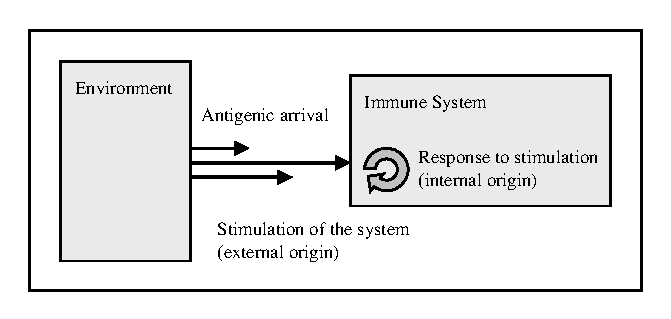
\includegraphics[scale=0.85]{Cells/antigenic-systemenv}
	\caption{Depiction of external stimulation resulting in internal activation.}
	\label{pic:cells:internalexternal}
\end{figure}

% virulence and amplitude
This \emph{exposure virulence} is a property of the antigen thus is not likely to change for a given immune system unless the antigen itself changes. The virulence may define the penalty for not identifying a antigen, as well as the amount of resultant specificity desired or required in a clonal selection and expansion response. This concern (virulence-specificity) is difficult to conceptualise as it defines the relative amount of refinement-based learning required of the system for a given antigen. The concern of the size of an antigen dose may be conceptualised as the amount or \emph{exposure amplitude} of information an antigen represents. The number of simultaneous antigen that arrive to the system in a given exposure defines the amount of work the system may have to support. The number of antigenic molecules that arrive in an exposure may be more than the number of lymphocytes in the repertoire. The result is that selection events may be more intense, resulting in the delay of some interaction until after the initial cells have proliferated or additional resources have been recruited. This \emph{exposure amplitude mismatch} scenario has two speculated implications: (1) Antigen may not be neutralised as quickly if it arrives in unexpectedly large quantities, that would result in the antigen arrival being considered a resources which must be degraded (neutralised over time), and (2) The increased selective pressure from the size mismatch may result in the rapid synthesis of a response large enough to address the exposure. This suggests dynamic and variable response size capabilities inherent in the clonal selection and expansion response. 

% why they are important
One may consider the effects of varied exposure virulence and amplitude on an immune system. Both properties affect the amount of work required in an immune response, although in different dimensions. Virulence may determine the desired specificity of a response such that high damage-causing pathogens are neutralised effectively and low damage-causing pathogens are neutralised with less specificity. The amplitude of the exposure defines the number of cells and the size of the clonal response. Therefore, the immune system must trade-off response strategies to the various anticipated virulence and amplitude combinations.
% implications for the system
For a single exposure event, an immune system is only concerned with quelling the antigen with a response. The scope of the concerns of an immune system for a single exposure is the specificity of the lymphocytes to the antigen and synthesising the cells in sufficient numbers. Initial antigen-identification (to trigger a response) may be assumed. Further, all resources of the repertoire may be allocated to the response for the exposure, as there are no future exposures. Iterations within a system under these conditions are concerned with adaptation in the context of a fixed and known single exposure event.

%
% Multiple Exposures
%
\subsubsection{Multiple Exposure Model}
A single exposure-response event may be abstracted to multiple antigen exposure-response events. A principle property of a multiple exposure regime is the temporal dimension it adds to such events. \emph{Exposure frequency} facilitates conceptualising multiple exposures as a series of atomic and quasi-independent single events, where the repetitiveness of the arrival of a given antigen is defined as its frequency. The exposure frequency may be measured as the pattern of \emph{exposure} and \emph{no-exposure} events in discrete time over an interval. The pattern may be defined as a probabilistic function, random, uniform, or may be a regular deterministic exposure function.
% effects of exposure frequency
The concept of a non-stimulation fostered by no-exposure events suggests a downtime when the immune system is not stimulated to respond. Such a non-activity event may also occur for an exposure event that is not identified by the exposed system. This inactive time is referred to as antigenic \emph{exposure downtime}. The activity of a system may be considered trigger-based in which learning and maintenance processes (such as cell aging and removal) only occur when the system is exposed to pathogen. During non-triggered periods, the system may enter a period of stasis awaiting subsequent triggers (the idle repertoire awaiting exposure model was criticised in the Immune Network Theory). An alternative model is that the system persists (always on), continuing to execute such maintenance processes in the absence of stimulation. The two models highlight the potential for the decoupling the system processes of \emph{repertoire maintenance} and \emph{repertoire stimulation}. Such a decoupled system would require an effective memory system such that acquired immunity (information) was not lost by the high-turnover of lymphocytes in the repertoire. The lack of adequate memory for this system type in an extended period of non-stimulation may cause the repertoire to devolve to a \naive\ (random) state. 

% variations of frequency
Variations in the exposure frequency control when the system can and must respond. Variations in the exposure amplitude control the size (scope or how much) of the response that a system must synthesise. Variations in exposure virulence and amplitude imply variations in a systems response strategy in terms of response specificity and response quantity. A similar relationship exists with multiple exposures with the addition of exposure frequency and the systems memory of the response. There is an inversely proportional relationship between immunological memory and exposure frequency (with constant virulence) such that when the exposure frequency is low, the memory must be long lived. When the exposure frequency is high, memory is short lived, and in fact may be satisfied with the quantity and specificity effects achieved from the single exposure without memory. One may consider the effect of combinations of high and low frequency exposures with high and low amplitude pathogen arrival. From a system perspective, the frequency and amplitude of exposures may be compressed (multiplicative relationship) into the amount of work (response effort) required for the interval of time. This compression of exposure frequency and amplitude may be referred to as the \emph{exposure regime} of an antigen to a system through time.

\begin{figure}[ht]
	\centering
	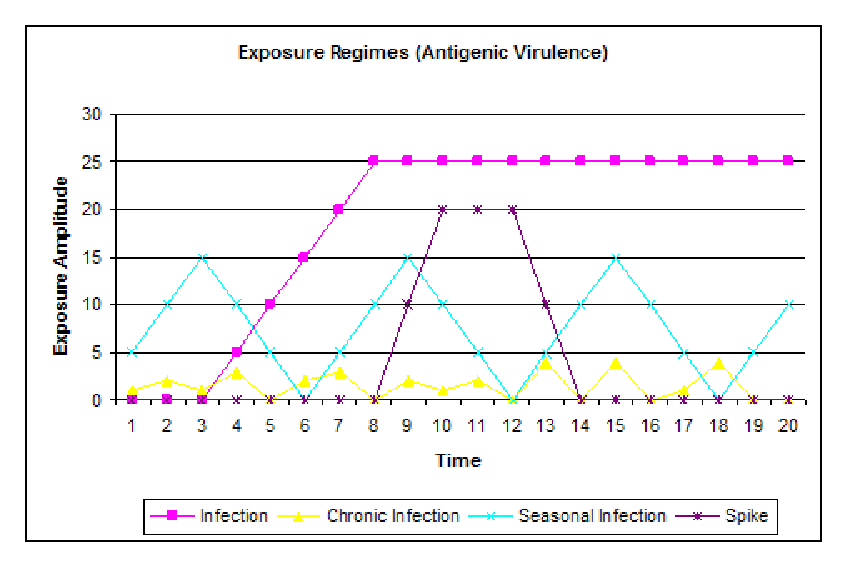
\includegraphics[scale=0.70]{Cells/exposures-virulence}
	\caption{Example exposure regimes demonstrating some archetypical pathogen virulence behaviours.}
	\label{pic:cells:virulence}
\end{figure}

% antigenic virulence
The relationship between a pathogen exposure regime and an immune systems response effort is interesting. For a single exposure event, virulence defined the amount of tissue damage an antigen may cause on a host, therefore it may provide a conception of the amount of specificity refinement (effort) required of an immune system for the exposure. An exposure regime provides a way of crisply defining \emph{antigenic virulence} (distinct from single exposure virulence) as a function of exposures through time. The amount of specificity refinement by the system for the antigen (response effort) is proportional to the exposure frequency and exposure amplitude (exposure regime). Antigenic virulence (and exposure regimes) may be expressed as an exposure amplitude graph against time. From this level of abstraction, one may give example exposure regimes as archetypical pathogen virulence strategies with which to subject an immune system (see Figure~\ref{pic:cells:virulence}). In addition to static antigenic virulence, it is possible for virulence to vary through time. The variance in virulence may be system-dependant such that virulence changes in response to the internal actions of the immune system such as in the case of an adversarial antigen (pathogen). 
% implications to the system
For a multiple exposure event, the system is primarily concerned with devising a response to each exposure and ultimately using past exposures to anticipate the resources needed for future exposures. This exposure model supersedes the single exposure event, as in the case of a single exposure, all resources of the repertoire are allocated to the specific concerns of the antigen (as there are no other antigens). The learning that the system may achieve within the context of a single exposure may be limited, as a broader exposure regime may define how often the exposures arrive to the system. The exposure regime may impose a quantity and specificity capability constraints for a single exposure, meaning that a finite amount of specificity learning and/or quantity learning may be achieved for a single exposure event. The system must learn to anticipate (1) the required specificity of future exposures, and (2) the required quantity of future exposures, both in the face of non-exposure events. 

% plots
\begin{figure}[htp]
	\subfloat[Single Exposure Model.]{
	\label{fig:cells:exposures:flowdiagram:single} %% label 
	\begin{minipage}[t]{0.50\textwidth}
		\centering 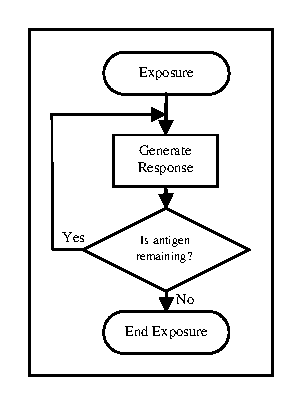
\includegraphics{Cells/exposures-single-model}
	\end{minipage}}%
	\hfill
	\subfloat[Multiple Exposure Model.]{
	\label{fig:cells:exposures:flowdiagram:multiple} %% label 
	\begin{minipage}[t]{0.50\textwidth}
		\centering 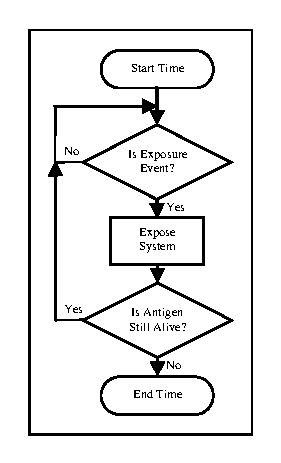
\includegraphics{Cells/exposures-multiple-model}
	\end{minipage}}\\
	% end
	\caption{Flow diagram of the single and multiple exposure models.}
	\label{fig:cells:exposures:flowdiagram} %% label for entire figure
\end{figure}

The exposure regime (frequency and amplitude) define the antigenic virulence and the systems required specificity. Repeated application of blind clonal selection facilitates improvement of a repertoire specificity for the antigen, and for a system that enters stasis during periods of non-stimulation (information acquired by the repertoire does not degrade), the density of information (clonal convergence and/or clonal densities) may define the quantity or scope of information required for the regime. Therefore, a repeated single selection on a relatively \naive\ repertoire fosters a model that matches the virulence of the antigenic exposure regime. For a repertoire with decoupled maintenance of cells and triggered adaptation, an explicit memory mechanism is required that retains acquired information proportional to the frequency of its exposure and complexity. For lower-complexity information, a more efficient strategy may be to generalise or re-acquired as need. 


%
% Multiple Antigen
%
\subsubsection{Multiple Antigen Model}
The natural extension of multiple antigen exposures is to subject an immune system to multiple concurrent exposure regimes. Each regime is expressed by a distinct \emph{antigenic type} or variety. Antigen types differ in their composition (surface features) such that the immune system has to acquire different immunity characteristics for each. In addition to the varied immunity characteristics, each antigen type has its own exposure regime, thus in the context of an immune system, the regime elicits a distinct response effort. The aggregation of multiple antigen types is an aggregation of multiple antigen exposure regimes to a given immune system that may collectively be referred to as the exposure or \emph{antigenic environment}. In responding to one given antigen, the repertoire may acquire a level of immunity (specificity) to another different and distinct pathogen type. This effect is called cross-reactivity of the immune response and may be conceptualised as reuse and generalisation of acquired information. One may consider an immune system to be exposed to the multiple different exposure regimes shown in Figure~\ref{pic:cells:virulence}. In this example, the system is exposed to all four different antigen with varied amplitudes at the discrete time of $t=11$. This may be referred to a \emph{concurrent antigen exposure}. Exposure concurrency requires that the repertoire is (1) large enough (with regard to the quantity of lymphocytes), and (2) diverse enough (with regard to lymphocyte specificity) to address multiple pathogen types at the same time. It is expected that the efficiency of the system will be reduced in such a situation, as resources are allocated proportional to the relative virulence of each antigen type. This effect highlights the requirement of the system to be able to not only respond to multiple antigen types at the same time, but to integrate the results of the concurrent responses (expanded clones and shifted the repertoire specificities).

Unlike the previous two models that were able to allocate all the resources of the repertoire to a single exposure of antigen information, multiple antigens requires a proportional allocation of resources to each antigen and its exposure regime. The proportionality of the response and allocation of repertoire resources is defined by the relative antigenic virulence to other antigen in its environment. The previous concerns of optimising specificity, quantity, and the anticipation of these values may be reduced to the systems adaptation of information densities toward exposure regimes. The density is representative of the learned (aggregated from experience) cell quantity (clone size) and specificity in the repertoire which facilitates anticipatory responses. Each cell has an affinity response surface (affinity landscape) for each pathogen it has been (and may be) exposed to. The clonal densities are acquired from the antigenic virulence which is defined as the amplitude and severity of exposures (amount of learning opportunity offered) to the system through time. This model provides the pinnacle in environments for clonal selection at the cellular level and a complement for the quintessential clonal selection framework.

%
% Exposure Models and Control
%
\subsubsection{Exposure Models and Control}
% general
The environment and the system may be considered two interdependent and required components of which neither is meaningful in isolation. In modelling these two components, one may consider the variable (configurable) aspects of each of which may or may not be within the control of a given simulation. 
% control
An intuitive example is to consider the environment (and therefore all aspects of antigen exposure) as outside of the scope of control, and all aspects of the system as inside of the scope of control. In this example the system must do all it can to cope with the specific properties of the exposures it is subjected to by the environment. The system must operate with finite resource, thus constraints are imposed on the control over aspects the system. This example may be extended further to consider that the evolution of antigen (pathogen) is influenced by the existence and evolution of the host system and that this relationship is reciprocal (co-evolution). Therefore, the system has influence (implicit influence via evolution) over aspects of antigen exposure over longer periods of time, and the antigen has influence (implicit influence via evolution) over aspects of the systems response over the same longer periods of time. This example may be generalised such that aspects of control are variable across both the environment and the system. 

\begin{figure}[ht]
	\centering
	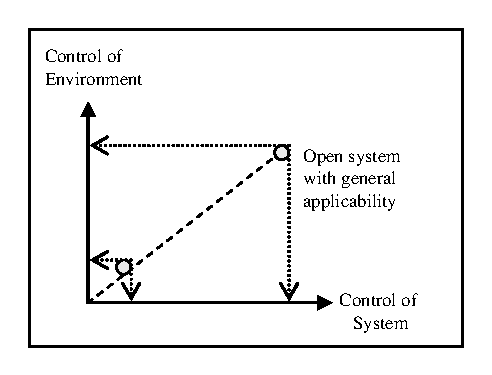
\includegraphics[scale=0.85]{Cells/exposures-tradeoff}
	\caption{Depiction of the trade-off between control of the environment and control of the system.}
	\label{pic:cells:tradeoff}
\end{figure}

% modelling control
In modelling \emph{environment} and \emph{system} and their \emph{interactions}, control may be exhibited over all aspects of both sides of the interaction. It is important to consider the influence for control or lack there of (constraints on control) on a system and its environment as it provides insight into the mapping of domain properties. A constraint may be considered the prior selection of a configuration parameter of a system or environment. The fixing of a configuration parameter in the environment influences the suitability of other unconstrained (controlled) parameters in the interaction, and the influence is likely to be complementary (such that fixing an aspect of the environment strongly influences the suitability of related parameters of the system and vice versa). This point highlights the symmetry of constraint between \emph{systems} and \emph{environments}, and the need to specialise a given system for the constraints of a given environment in which it is to be deployed (mapped problem domain).

%
% Colour Space Domain
%
\subsection{Colour-Space Domain}
\label{subsec:cells:paradigm:colourspace}
In his book detailing the Cognitive Theory of acquired immunity, Cohen used an example of cellular degeneracy in the retina as an analogy for the degeneracy of cell-bound receptors in the immune system \cite{Cohen2001a}. Cohen described how individual cells in the retina have limited capability, responding to constrained wavelengths of light, although from these specific degenerate detectors higher-level information such as a coherent image can be perceived through aggregation. The Self-Organizing Map (SOM) is a competitive and unsupervised learning algorithm that is renowned for its feature extraction and dimensionality reduction capabilities (see Section~\ref{subsec:cs:related:competitive}). In his doctoral work, Honkela used a colour domain (red-green-blue or RGB), and a dataset of known colours in that domain \cite{Honkela1997} (page 14-18). The learning and ordering of the domain of RGB colours based on the dataset was used as an intuitive example of the topological preserving properties of the SOM algorithm. Although Honkela may not have been the first to employ this example domain to the SOM, it has become a canonical example domain.\footnote{There are many applet and tutorial web sites on the Internet that use this example to demonstrate the SOM, the listing of which is not necessary.} Inspired by the simplicity and suitability of the colour domain to qualitatively (visually), and quantifiably (numerical measures) demonstrate the properties of the SOM, this section defines a \emph{colour-space} domain from which a suite of test problem instances may be drawn to investigate clonal selection. Inspired by Cohen's analogy to the retina, colour-space is named for the relationship to the shape-space formalism, and is supported by proven use of the same principle for a related Competitive Learning paradigm.

%
% Contrived Domain
%
\subsubsection{Domain Definition}
The domain does not provide a framework for investigating the so-called colour space theory, which refers to the study of colour models used in display and printer systems. Nor is the intention of the defined test domain for the study of colour theory, the investigation of colour segregation, colour recognition, palette compression, or colour clustering (or any other practical colour-based application domain). Given what the intentions are not, this section outlines a series of general goals for designing a test domain for adaptive systems, followed by the definition of a simple colour-space domain that meets these goals. The ambition is to contrive a domain from which trivial problem instances can be drawn to preliminary assess specific properties of adaptive models. These models may be engaged in processes that equate to pattern recognition and optimisation, and may involved the evaluation of broad characteristics such as learning, memory, and adaptation. See Table~\ref{tab:cells:colourspace:goals} for a list of the general design goals (requirements) for a problem domain suitable for this purpose.

\begin{table}[ht]
	\centering\small
		\begin{tabularx}{\textwidth}{lX}
		\toprule
		\textbf{G\#} & \textbf{Goal} \\ 
		\toprule
		G1 & The domain must provide a numerical and/or combinatorial basis that may be manipulated meaningfully by operators. \\ 
		\midrule
		G2 & The response surface must be correlated such that localised regions in the response surface have a gradient. \\ 
		\midrule
		G3 & The domain must be suitable for optimisation tasks.  \\ 
		\midrule
		G4 & The domain must be suitable for pattern recognition tasks. \\ 
		\midrule
		G5 & The domain must be parameterised such that the relative complexity may be meaningfully adjusted. \\ 
		\midrule
		G6 & The domain must be easily and meaningfully visualised both online (dynamically) and off-line (end of run). \\ 
		\midrule
		G7 & The domain must be easy to understand, easy to implement, and easy to analyse. \\ 
		\midrule
		G8 & The properties of the domain (e.g. the response surface or visualisation) should facilitate rather than mask model behaviours being investigated. \\ 
		\bottomrule
		\end{tabularx}	
	\caption{List of goals for a colour-space domain.}
	\label{tab:cells:colourspace:goals}
\end{table}

The colour-space domain formalism meets the list of goals proposed in Table~\ref{tab:cells:colourspace:goals}. The formalism is comprised of a series of terms to describe the characteristics of a colour space domain. The characteristics identified include the environment: the cardinality, the representation, and the mapping function (see Table~\ref{tab:cells:colourspace:definition} for their definition and summary).

\begin{table}[ht]
	\centering\small
		\begin{tabularx}{\textwidth}{llX}
		\toprule
		\textbf{Term} & \textbf{Name} & \textbf{Summary} \\ 
		\toprule
		$E$ & Environment & The search space (colour space) which defines the scope of feasible coordinates defined by its dimensionality (1-$n$), a boundary (limits of each dimension), and cardinality ($C$). \\ 
		\midrule
		$R$ & Representation & An encoding used and manipulated by adaptive models. It may be binary, integer, real, and may or may not directly represent a coordinate in the colour space ($E$). \\ 
		\midrule
		$M$ & Mapping Function & Converts a given representation ($R$) into a coordinate in the colour space ($E$). If the representation used matches the coordinate system of the environment, then the mapping function returns an unchanged coordinate. \\ 
		\midrule
		$C$ & Cardinality & The number of discrete points in the domain, and ideally (given display capabilities) the number of colours available for visualisation. \\ 
		\midrule
		$I$ & Intention & The goal of a system within the domain, a task or action it is to perform or achieve. This is a cover-all term for something to do in a defined colour-space. \\ 
		\bottomrule
		\end{tabularx}	
	\caption{Summary of terms for the colour space domain formalism.}
	\label{tab:cells:colourspace:definition}
\end{table}

The environment ($E$) is an $n$-dimensional hypercube (for visualisation purposes perhaps limited to 1-3 dimensions), where each dimension represents a different colour axis. The intention is that a distinct coordinate in a given environment (colour space) represent a distinct colour. For example, a monochrome (one-colour) environment would be implemented as a one-dimensional space (line) perhaps a gradient of white to black. An RGB colour space would be implemented as a three-dimensional (cube) environment. An environment is a volume of feasible discrete points, and the cardinality ($C$) defines the number of points in that volume. The granularity of each dimension in the environment also determines the number of colours, thus cardinality may be thought of as the palette of the environment. Further, the palette analogy may be exploited further in defining standard cardinalities, such as those common palettes that are used in computer display systems (for example, 8-bit colour ($2^{8}$) with a pallet of 256 colours). The coordinate-based representation ($R$) may be used directly by an adaptive system. Alternatively a symbolic or sub-symbolic representation may be used (such as bit-strings), which require a mapping function ($M$) to transform representation into a given environments coordinate system. 
The task of an adaptive system is called an intention ($I$), examples may include the optimisation of a randomly initialised system to a set of pre-selected points, or the adaptation of a system to a defined region within the environment.

One may measure the Euclidean distance between points in the colour space as a quantitative measure of difference. Distances measures may not be limited to Euclidean distance, for example Manhattan distance (and many others, see \cite{Kohonen2001} pages 17-29) may be used in the colour space. Distance measures may be augmented with coordinate radii such that a point of interest in the space may represent a collective of points in its vicinity. Such regions may be defined as hyper-cubes or spheres, and may have a distance-based falloff such as linear, Gaussian or exponential. These distances and coordinate neighbourhoods are also qualitatively meaningful. Following a line (for example in a monochrome or RGB) in colour space shows a transition through intermediate colour coordinates (colours). These intermediate colours are quantifiably distinct (numerical coordinates), and qualitatively different (assuming the colour transition can be detected by the human eye). This correlation is also useful for visualisation: agents representing coordinates in the colour space may be implemented, which may permit qualitative measures and observations of system behaviour. 

%
% Illustrative Examples
%
\subsubsection{Illustrative Examples}
This section proposes an \emph{optimisation}, \emph{pattern recognition}, and \emph{classification} examples of Colour Space Problems that adaptive systems that may be employed or extended to investigate adaptive models. 

\begin{itemize}
	\item \emph{Optimisation}: Involving the pre-selection of a coordinate in the space that is withheld from the adaptive system, and defining a cost function as a distance measure to the given coordinate. For example if a space was defined as an 8-bit one-dimensional domain (0-255), a goal coordinate of 127, and an Euclidean distance measure employed as a cost function, then the shape of the response surface would be a triangle with the apex at the selected coordinate. 
	\item \emph{Pattern Recognition}: The optimisation domain may be generalised with a set of goal coordinates (Colour Space Patterns) to which a given system is exposed. The intention of the system for this problem is to optimise (optimally match) the set of patterns, where the order of exposure of the patterns to the system is also withheld from the system.
	\item \emph{Classification}: A classification task may be defined as an extension of the pattern recognition problem with the addition of categorical information. A geometry can be defined within the colour space and class labels can be assigned to the resulting concave regions. In addition to distance-based feedback, the system may be provided with corrective categorical based feedback, relaxing the optimisation of the goal coordinates to that of accuracy of predicting pattern classes.
\end{itemize}


%
% Criticisms and Limitations
%
\subsubsection{Criticisms and Limitations}
This section addresses the important consideration's of the limitations of the formulated problem domain, as follows:

\begin{enumerate}
	\item \emph{Triviality}: The domain and resultant problem definitions are primitive. The problem instances are likely easily solved rapidly by standard deterministic techniques, and even by \naive\ approaches such as enumeration and random search.
	\item \emph{Transferability}: The results achieved on one or a set of derived problem instances are very likely to be not transferable to problem domains of interest (difficult, real-world). Conclusions regarding model performance are limited to the instances on which they are tested, and perhaps related trivial domains.
	\item \emph{Difficulty}: Although superficiality they appear trivial, there is no innate sense of the absolute or relative difficulty of the derived problem definitions.
	\item \emph{Visibility}: For high-cardinality domains (such as those at or above 24-bit or 32-bit RGB) the human eye cannot detect colour differences between coordinates within close proximity.
	\item \emph{Novelty}: The colour space domain and derived problem instances are not novel, they are generalisations and simplifications of existent test domains and benchmark problems.
\end{enumerate}

It is prudent not to rebut these criticisms, but to acknowledge them as limitations (designed or otherwise) of the domain and framework that it provides. The domain and resultant problem instances are intended to be trivial (easy to solve) such that the attention remain on the model under study. The performance of a given model is not intended to be transferable, what is expected to be transferable are the general functional behaviours that the domain assists in isolating and assessing. The relative difficulty of problem instances may be determined by baseline strategies. Comparable relative and absolute difficulty may be defined using the tools of probability, statistical mechanics, and additional (suitable) mathematical apparatus. The visual distinctiveness of close-proximity coordinates in high-cardinality spaces may be exaggerated where appropriate. For example, a dynamically normalised colour scale may be allocated to coordinates of interest. Finally, novelty is not claimed, rather the domain is a \emph{consistent reformulation} of classical optimisation and pattern recognition benchmark domains.

%
% Realised Cellular Paradigm
%
\section{Realised Cellular Paradigm}
\label{sec:cells:realised}
This section provides a realisation of the concerns of the abstract \emph{Cellular Clonal Selection Paradigm} presented in Section~\ref{sec:cells:paradigm}. This includes general definitions of a standardised problem domain in the Antigenic Exposure Problem as a specialisation in colour space, and the Cellular Clonal Selection Algorithm that provides a basis for investigation into elaborated cell interaction schemes. A series of cell-based measures are presented for assessing cellular algorithms on instances of Antigen Exposure Problems that provide quantitative indicators regarding the concerns of information acquisition and application. Collectively, this section provides a basis for the implementation and exploratory empirical investigation into the Cellular Clonal Selection Paradigm, as well as a bridge between the biology (Section~\ref{sec:cs:theory}) existing approaches (Section~\ref{sec:cs:algorithms}), and the abstract clonal selection and antigenic exposure models (Section~\ref{sec:cells:paradigm}).


%
% Antigenic Exposures
%
\subsection{Antigenic Exposures}
\label{sec:cells:realised:exposures}
This section considers the realisation of the specialisations of the exposure paradigm outlined in Section~\ref{subsec:cells:paradigm:antigenicexposures} as a basis for empirical investigation and ultimate application of cellular models to problem domains. This realisation includes the definition of general antigenic exposure problem with exposure regimes, and a specialisation to the colour space domain.

%
% Antigenic Exposure Problem 
%
\subsubsection{Antigenic Exposure Problem}
% general nomenclature
For the purposes of discussing exposure, a cellular clonal selection algorithm may be reduced to its information content, distinct from the specific clonal selection processes operating upon that information. Specifically, a cellular algorithm may be considered a population or repertoire ($T$, that stands for `tissue' which will be made apparent in proceeding chapter) of discrete cells ($C$), as follows: $T = \{C_1, C_2, C_3 \ldots, C_n\}$. Therefore an \emph{Antigenic Exposure Problem (AEP)} is defined as the discrete interaction with a $T$, with a set ($I$, which stands for `infection') of antigen ($A$) at the same level of abstraction, as follows $I = \{A_1, A_2, A_3 \ldots, A_n\}$. An antigen is comprised of sub-antigenic information referred to as determinants ($D$), such that $A = \{D_1, D_2, D_3 \ldots, D_n\}$. 

\begin{algorithm}[ht]	
	\SetLine
	
	\SetKwFunction{StopCondition}{StopCondition}	
	\SetKwFunction{CreateRandomAntigen}{CreateRandomAntigen}
	\SetKwFunction{Exposure}{Exposure}
	
	\SetKwData{Infection}{I}
	\SetKwData{Tissue}{T}
	
	\KwIn{\Tissue, $N_{determinants}$ $N_{antigen}$}
	\KwOut{$T_{rs}$}
	
	% prepare
	\Infection $\leftarrow$ 0\;
  \For{i$\leftarrow$0 \KwTo $N_{antigen}$}
  {
  	$A_i \leftarrow$ \CreateRandomAntigen{$N_{determinants}$}\; 
  	\Infection $\leftarrow A_i$\;
  }  
  % exposures
  $T_{rs} \leftarrow$ 0\;
	\While{$\neg$\StopCondition{}}
	{
		$T_{rs} \leftarrow$ \Exposure{\Infection, \Tissue}\;
	} 
	\Return{$T_{rs}$}\;
	\caption{Antigenic Exposure Problem (AEP).}
	\label{alg:cells:realised:exposures:aep}
\end{algorithm}

% algorithm
Algorithm~\ref{alg:cells:realised:exposures:aep} defines a simple antigenic exposure problem, with symmetrical information content for interaction with a given cellular system, where $N_{determinants}$ and $N_{antigen}$ define the number of determinants per antigen and total antigen within the scope of the AEP. The algorithm clearly shows the AEP's in control of the interactions with a given $T$, where discrete interactions are mediated via an $Exposure(I,T)$ operation. The algorithm definition also highlights that from an exposure perspective, the AEP is only concerned with a systems aggregate responses to exposures. The tissue result set denoted as $T_{rs}$ may be considered to represent a cellular algorithm's ($T$) capability to address a given antigen exposure problem ($I$).

%
% Cellular Exposure Regimes
%
\subsubsection{Cellular Exposure Regimes}
The defined antigenic exposure problem delegates the specifics of algorithm-problem interaction to the $Exposure(I,T)$ operation, the behaviour of which may be referred to as a \emph{Cellular Exposure Regime (CER)}. For example, the information content of the problem may be exposed to a system (1) consistently in the same order, (2) in a randomised order, or (3) in some biased manner resulting in an asymmetric perspective of such information content. Referring to such interactions as an exposure regimes also highlights the important point that the cellular algorithm is considered a passive information processing system that responds to the active exposure of antigenic stimuli. Therefore, depending on the specific problem domain, the concerns of exposure, re-exposure, and multiple exposures (from Section~\ref{subsec:cells:paradigm:antigenicexposures}) may or may not be within the scope of control of the system. Algorithm~\ref{alg:cells:realisation:exposure:aep:cer} provides an example of a regular and consistent exposure regime $Exposure(I,T)$ operation where a system is exposed and must respond to the scope of the AEP each $I$ exposure called an epoch. The example also delegates the responsibility of specific cell interaction (selection and response) to the cellular clonal selection algorithm in the $Exposure(A,T)$ operation. This operation encapsulates the scope of concerns of algorithms in the cellular paradigm.

\begin{algorithm}[ht]	
	\SetLine
	\SetKwFunction{Exposure}{Exposure}	
	\SetKwData{Infection}{I}
	\SetKwData{Tissue}{T}
	
	\KwIn{\Infection, \Tissue}
	\KwOut{$T_{rs}$}
	
  % exposures
  $T_{rs} \leftarrow$0\;
	\ForEach{$A_i \in $ \Infection}
	{		
		$C_{i} \leftarrow$ \Exposure{$A_i$, \Tissue}\;
		$T_{rs} \leftarrow C_{i}$\;
	} 
	\Return{$T_{rs}$}\;
	
	\caption{Exposure Function (CER) for the Antigenic Exposure Problem.}
	\label{alg:cells:realisation:exposure:aep:cer}
\end{algorithm}


% the unknowns for a CCSA
The cellular exposure regime represents the uncertainty in the information processing faced by a cellular algorithm, including but not limited to (1) the number of antigen ($N_{antigen}$), (2) the number of determinants for a given antigen ($N_{determinants}$), the diversity of the information in the antigenic environment ($I$), and the ordering of the discrete information exposures defined in the the exposure regime itself (CER). Finally, discrete cellular interactions with antigen and determinants may not yield specific information, rather a general indication. For example from an abstract point of view an $Exposure(A, C)$ or $Exposure(D, C)$ may result in a relative indication of fit or suitability (affinity or avidity) rather than absolute cost. This is motivated by the pre-committed, iterative, and trial-based (selectionist) strategy reduced from the clonal selection theory.

%
% Antigen Colour Space Problem
%
\subsubsection{Antigen Colour Space Problem}
% colour space
The antigenic exposure problem may be specialised in the colour space domain as a pattern recognition problem called the \emph{Antigen Colour Space Problem (ACSP)}. The problem is defined as a set of Colour Space Patterns (CSP) each of which is defined as a colour comprised of three 64-bit colour components. The set of patterns are generated as a set of random binary strings ($A\prime = \{0,1\}^{L}$, where $L=(3\times64)$) and decoded using the Gray Code method for each colour component (Equation~\ref{eq:cells:realised:graycode}, where $\bigoplus $ denotes addition modulo two) to a three dimensional colour vector $A = [0,1]^{3}$. Cellular solutions ($C$) to each antigen colour space pattern ($A$) are 192-bit binary strings that decoded to 3-dimensional colour vectors using Gray Code. The affinity (avidity) function for a decoded cell, the $Exposure(A, C)$ is defined as the Euclidean distance between the two vectors (Equation~\ref{eq:cells:realised:euclidean}).

% Gray Code
\begin{equation}
	GrayCode(A\prime) = \frac{1}{2^{64}-1} \left(\sum_{j=0}^{64-1} \left(\bigoplus_{k=1}^{64-j}A\prime(i-1) 64+k\right) 2^j\right)
	\label{eq:cells:realised:graycode}
\end{equation}

% Euclidean Distance
\begin{equation}
	EuclideanDistance(A, C) = \sqrt{\sum_{i=1}^n  \left(A_i - C_i\right)^2}
	\label{eq:cells:realised:euclidean}
\end{equation}

% minimum
This mapping of the colour space problem onto the antigenic exposure problem highlights the important point of the minimal cases of the problem, specifically: (1) minimum determinant, and (2) minimum antigen. From an abstract perspective, a cell matches onto one determinant, from an antigen of multiple determinants. Therefore, from a system perspective a one-to-one relationship exists between a given cell and its cognate antigen mediated via the specific sub-feature (antigenic determinant). A \emph{Minimum Determinant Antigenic Exposure Problem (MDAEP)} may be defined where each antigen is comprised of a single determinant ($N_{determinants}=1, \forall A \in I$). This case forces such a one-to-one relationship at the cost of the exclusion of the cross-reactivity of cells. In the same manner, the number of antigen in the set may be minimised ($N_{antigen}=1$) to define a \emph{Minimum Antigenic Exposure Problem (MAEP)} where a given system $T$ is assessed based on its capability with a single antigen with a single determinant. This minimal case (single or multiple exposures of a single determinant), provides a minimal context in which to consider fundamental behaviours of cellular algorithms and their extensions.

%
% Cellular Clonal Selection
%
\subsection{Cellular Clonal Selection}
\label{sec:cells:realised:algorithms}
This section considers the realisation of specialisations of quintessential clonal selection outlined in Section~\ref{subsec:cells:paradigm:clonalselection} as a basis for empirical investigation and ultimate application of cellular models to problem domains. This realisation includes the definition of a general cellular clonal selection algorithm as a homologue to CLONALG, and a replacement based extension.

%
% Cellular Clonal Selection Algorithm
%
\subsubsection{Cellular Clonal Selection Algorithm}
% general
A \emph{Cellular Clonal Selection Algorithm (CCSA)} is defined as the application of the computational properties of the clonal selection theory constrained by the concerns of the theory at the cellular-level. These constraints include but are not limited to (1) the interaction with antigen via their determinants, (2) the embodiment of information in a self-contained repertoire of discrete cells, and (3) the cellular response to active antigenic exposures. The extent of the taxonomy of clonal selection algorithms reviewed in Section~\ref{sec:cs:algorithms} may be considered to reside in the cellular level (within the scope of the Cellular Clonal Selection Paradigm).
% abstraction
This section considers an abstraction of cellular clonal selection algorithms in the context the concerns considered in quintessential Clonal Selection in Section~\ref{subsec:cells:paradigm:clonalselection}. The Antigen Exposure Problem defined a cellular system in terms of its information content, where the problem is the active concern and the cellular system is passive until exposed with stimuli to which it reflexively responds. The scope of the concerns of cellular clonal selection algorithms are the management of information within the repertoire, and in particular the management of information under the discrete exposures of an AEP.

\begin{algorithm}[ht]
  \SetLine
  \SetKwData{T}{T}
  \SetKwFunction{CreateCell}{CreateCell}   
  \KwIn{$N_{cells}$}		
  \KwOut{\T}  
  
	\T $\leftarrow$ 0\;	
	\For{i$\leftarrow$0 \KwTo $N_{cells}$}
	{
		$C_i \leftarrow$ \CreateCell{}\;
		\T $\leftarrow C_i$\;
	}
	\Return{\T}\;
	\caption{Initialisation Function for the Cellular Clonal Selection.}
	\label{alg:cells:realisation:algorithms:ccsa:init}
\end{algorithm}

% algorithm
Algorithm~\ref{alg:cells:realisation:algorithms:ccsa:init} defines an initialisation operation for a the Cellular Clonal Selection Algorithm, where the $CreateCell()$ may be specialised to create random cells with a representation appropriate for the specific problem domain (192-bit binary strings in the case of the ACSP). Algorithm~\ref{alg:cells:realisation:algorithms:ccsa:exposure} defines the $Exposure(A, T)$ operation for the CCSA that provides a generalisation of the CLONALG, BCA, AIRS, and IA family of the reviewed clonal selection taxonomy. Specifically, the algorithm responds to antigen exposures by assessing the extent of the repertoire and selecting a subset ($N_{selected}$) to comprise a response. Each cell in the selected set creates a set of clones ($N_{clones}$) with mutations ($P_{mutation}$) that are assessed against the antigen and compete with the progenitor of the selected set for a position in the repertoire. This generalisation which strongly resembles CLONALG, implicitly manages the memory cell set and explicitly returns a best matching cell ($GetBestMatchingCell(T)$) for each exposure as the most suitable response within the scope of the repertoire. Importantly, the CCSA provides the flexibility to assume a variety of configurations, specialisations (such as the CSA taxonomy), as well as the extensions considered in this chapter.

% CCSA
\begin{algorithm}[ht]
  \SetLine	
  
  \SetKwData{Antigen}{A}
	\SetKwData{Tissue}{T}
  
	\SetKwFunction{Clone}{Clone}
	\SetKwFunction{Mutate}{Mutate}
	\SetKwFunction{Select}{Select}
	\SetKwFunction{Expose}{Expose}
	\SetKwFunction{GetBestMatchingCell}{GetBestMatchingCell}
	\SetKwFunction{Remove}{Remove}
	\SetKwFunction{Add}{Add}
	
  \KwIn{\Antigen, \Tissue, $N_{selected}$, $N_{clones}$, $P_{mutation}$}
	\KwOut{$T_{rs}$} 
	
 	% exposure
 	$T_{rs} \leftarrow0$\;
 	\ForEach{$C_i$ $\in$ \Tissue}
 	{
 		\Expose{\Antigen, $C_i$}\;
 	}
	% selection
	$T_{selected} \leftarrow$ \Select{\Tissue, $N_{selected}$}\;
	% cloning and competition
	\ForEach{$C_i$ $\in$ $T_{selected}$}
	{
		% clone and mutate
		$T_{clones} \leftarrow 0$\;
		\For{i$\leftarrow$0 \KwTo $N_{clones}$}
		{
			${C\prime}_i \leftarrow$ \Clone{$C_i$}\;
			${C\prime}_i \leftarrow$ \Mutate{${C\prime}_i$, $P_{mutation}$}\;
			$T_{clones} \leftarrow {C\prime}_i$\;
		}
		% expose clones
		\Expose{\Antigen, $T_{clones}$}\;
		% select the set
		${T\prime}_{clones} \leftarrow$ \Select{$T_{clones}$, $N_{selected}$}\;
		% competition for position
		\For{i$\leftarrow$0 \KwTo $N_{selected}$}
		{
			$C_{selected} \leftarrow {T_{selected}}_i$\;
			$C_{clone} \leftarrow {{T\prime}_{clones}}_i$\;
			\If{$C_{clone}$.score $\leq C_{selected}$.score}
			{
				\Tissue.\Remove{$C_{selected}$}\;
				\Tissue.\Add{$C_{clone}$}\;
			}
		}
	}
	% select bmu
	$T_{rs} \leftarrow$ \GetBestMatchingCell{\Tissue}\;
	\Return{$T_{rs}$}
	\caption{Exposure Function for the Cellular Clonal Selection.}
	\label{alg:cells:realisation:algorithms:ccsa:exposure}
\end{algorithm}

% minimal
The CCSA may be reduced to a minimal configuration to provide a complement to the Minimal Antigenic Exposure Problem called the \emph{Minimal Cellular Clonal Selection Algorithm (MCCSA)}. This minimal configuration under the MAEP provides a realisation of of the ES$(1+1)$ algorithm and connection with mutation based hill climbers made in Section~\ref{sec:cs:related}. For example, ES$(1+1)$ would be defined by the configuration: $N_{cells}=1$, $N_{selected}=1$, $N_{clones}=1$, and $P_{mutation}=\frac{1}{L}$.

%
% Replacement Cellular Clonal Selection Algorithm
%
\subsubsection{Replacement Cellular Clonal Selection Algorithm}
An expected effect with the Cellular Clonal Selection Algorithm is that it results in the iterative adaptation of specialised and independent cells. This is expected (1) because it was observed in CLONALG with regard to a niching-like effect, and (2) because CCSA and CLONAL resemble a parallel mutation based hill climber. The \emph{Replacement Cellular Clonal Selection Algorithm (RCCSA)} defined in Algorithm~\ref{alg:cells:realisation:algorithms:rccsa:exposure} is an extension of the CCSA where all clones created for an exposures are aggregated into a clonal set, which then competes with the cells in the repertoire on a per-cell basis for a limited position in the repertoire. This `clonal set-repertoire competition' is intended to provide more opportunity for per-exposure resource allocation, by allowing clones to compete and potentially displace repertoire members that may or may not be the clonal progenitor (progenitor of clones), clonal siblings (same progenitor), or exposure clonal siblings (same exposure). This competition is promoted firstly through a cell-to-cell distance assessment that simulates the competition the cells face during selection by antigen where similar cells compete for the same antigenic patterns, and in the affinity comparison that selects those cells that respond better to the specific antigen to which the system has been exposed. This competition mechanism decouples intra-repertoire competition for survival in the integration of clones from the antigenic-based selection that resulted in the creation of the clones. Such decoupling may be exploited in the integration of cells with varied origins. 

\begin{algorithm}[ht]
  \SetLine
  \SetKwData{Antigen}{A}
	\SetKwData{Tissue}{T}

	\SetKwFunction{Clone}{Clone}
	\SetKwFunction{Mutate}{Mutate}
	\SetKwFunction{Select}{Select}
	\SetKwFunction{Expose}{Expose}  
  \SetKwFunction{Remove}{Remove}
	\SetKwFunction{Add}{Add}
	\SetKwFunction{Distance}{Distance}
	\SetKwFunction{GetBestMatchingCell}{GetBestMatchingCell}
	
  \KwIn{\Antigen, \Tissue, $N_{selected}$, $N_{clones}$, $P_{mutation}$}
	\KwOut{$T_{rs}$} 	
	
 	% exposure
 	$T_{rs} \leftarrow$0\;
 	\ForEach{$C_i \in$ \Tissue}
 	{
 		\Expose{\Antigen, $C_i$}\;
 	}
	% selection
	$T_{selected} \leftarrow$ \Select{$T$, $N_{selected}$}\;
	$T_{clones} \leftarrow$0\;	
	% cloning and mutation
	\ForEach{$C_i \in T_{selected}$}
	{
		% clone and mutate
		\For{i$\leftarrow$0 \KwTo $N_{clones}$}
		{
			${C\prime}_i \leftarrow$ \Clone{$C_i$}\;
			${C\prime}_i \leftarrow$ \Mutate{${C\prime}_i$, $P_{mutation}$}\;
			$T_{clones} \leftarrow {C\prime}_i$\;
		}
	}
	% expose clones
	\Expose{\Antigen, $T_{clones}$}\;		
	% competition for position
	\For{$C_{clone}$ \KwTo $N_{clones}$}
	{
		% locate most similar
		$C_{selected} \leftarrow 0$\;
		\ForEach{$C_i \in T$}
		{			
			\If{\Distance{$C_{clone}$, $C_i$} $<$ \Distance{$C_{clone}$, $C_{selected}$}}
			{
				$C_{selected} \leftarrow C_i$\;
			}
		}
		% compete		
		\If{$C_{clone}$.score $\leq C_{selected}$.score}
		{
			\Tissue.\Remove{$C_{selected}$}\;
			\Tissue.\Add{$C_{clone}$}\;
		}
	}	
	% select bmu
	$T_{rs} \leftarrow$ \GetBestMatchingCell{\Tissue}\;
	\Return{$T_{rs}$}\;
	
	\caption{Exposure Function for Replacement Cellular Clonal Selection.}
	\label{alg:cells:realisation:algorithms:rccsa:exposure}
\end{algorithm}


%
% Empirical Assessment
%
\subsection{Empirical Assessment}
\label{sec:cells:realised:measures}
This section defines a series of general empirical measures that provide instantaneous information regarding a given CCSA on colour space specialisations of the Antigenic Exposure Problem. An important consideration of these measures in the context of investigation via exploratory experimentation is not their absolute value, but rather their relative change in value with changes to the systems being investigated. Two general classes of measures are considered, (1) error measures that assess the capability of a system in the context of a given problem instance, and (2) diversity measures that consider the general state of the information content within a given system.

%
% Average Cell Error (ACE)
%
\subsubsection{Average Cell Error}
The error of a cell may be assessed as its affinity for a given antigen, and may be assessed using the problem domains specific $Exposure(A, C)$ operation, in this case Euclidean Distance (defined in Equation~\ref{eq:cells:realised:euclidean}). Although not used directly, \emph{Cell Error (CE)} (defined in Equation~\ref{eq:cells:realisation:measure:ce}) provides an error-centric buillding building block for addition error assessments.

% Cell Error
\begin{equation}
	CellError(A,C) = EuclideanDistance(A, C)
	\label{eq:cells:realisation:measure:ce}
\end{equation}

An important application of Cell Error is its calculation for each cell in in the result set ($T_{rs}$) returned from a cellular algorithms $Exposure(I, T)$ operation. The Average Cell Error (ACE) defined in Equation~\ref{eq:cells:realisation:measure:ace} is a problem specific (ACSP) measure for assessing the general capability of a cellular algorithm on an antigenic exposure problem.

% Average Cell Error
\begin{equation}
	AverageCellError(I,T_{rs}) = \frac{1}{I_n} \sum_{i=1}^{{T_{rs}}_n} CellError(A_i, C_i)
	\label{eq:cells:realisation:measure:ace}
\end{equation}

%
% Average Cell Diversity (ACD)
%
\subsubsection{Average Cell Diversity}
A diversity measure of the cellular repertoire provides some indication of the variation in the discrete information stored within the repertoire. Low diversity reflects a homogeneous repertoire, whereas high diversity reflects a heterogeneous set of cells. Given the selected bit string basis of the CCSA, diversity between two cells may be measured as the hamming distance between the cells (see Equation~\ref{eq:cells:realisation:cd}, where Hamming Distance is defined in Equation~\ref{eq:cells:realisation:hamming}, and $\oplus$ denotes exclusive-or (XOR).

% Hamming Distance
\begin{equation}
	HammingDistance(X, Y) = \sum_{i=1}^L \left( X_i \oplus Y_i \right)
	\label{eq:cells:realisation:hamming}
\end{equation}

% Cell Diversity
\begin{equation}
	CellDiversity(C1, C2) = HammingDistance(C1, C2)
	\label{eq:cells:realisation:cd}
\end{equation}

Cell Diversity (CD) can be calculated for each cell in the repertoire against all other cells in the repertoire to provide an indication the average number of bit differences of a given cell to the rest of the cells in the repertories, called the Average Cell Diversity (ACD) defined in Equation~\ref{eq:cells:realisation:acd}.

% Average Cell Diversity
\begin{equation}
	AverageCellDiversity(T) = \frac{1}{T_n}\sum_{i=1}^{T_n} \left(\frac{1}{T_n}\sum_{j=1}^{T_n} CellDiversity(C_i, C_j)\right) 	
	\label{eq:cells:realisation:acd}
\end{equation}


%
% Trends and Behaviours
%
\subsection{Trends and Behaviours}
\label{sec:cells:realised:trends}
This section considers the expected emergent effects and behavioural trends of cellular-based clonal selection algorithms as defined in the specific realisations.

%
% Primitive Behaviour Trends
%
\subsubsection{Primitive Behaviour Trends}
The foundational expectation is that the realised Cellular and Replacement Clonal Selection Algorithm behave much like CLONALG and AIRS. Specifically, that the algorithm will acquire information via selection and adaptation. This section outlines the specific foundational behaviour trends of the algorithms in the context of the pressures and principles of the clonal selection strategy discussed in Section~\ref{subsec:cells:paradigm:clonalselection}.

\begin{enumerate}
	\item \emph{Repertoire Size}: The repertoire size must be sufficiently large to ensure that selection of cells and integration of clones do not result in competition between cells specialised for different antigen. Such competition by an insufficiently sized repertoire is expected to result in unstable behaviour. 
	\item \emph{Selection Size}: The number of clones selected per antigen exposure defines the amount of resources allocated to each antigen under fixed clonal integration. An increase in resource allocation via an increase in selection is expected to result in increased specialisation via the promotion of `concurrent redundant perspectives' of a given antigen. 
	\item \emph{Cloning Size}: The number of clones created per selected cell reflects the amount of computational effort expended on re-sampling modifications on a `known-to-be-good' structure. Therefore an increase in cloning and acceptance of limited high-affinity clones is expected to result in an increased specialisation toward exposed antigen. 
	\item \emph{Replacement Constraints}: Replacement constrained by a clonal progenitor is expected to result in a constrained and specialised hill climbing-like behaviour (MHCA). The relaxation of this constraint such that clonal progeny compete directly with the repertoire is expected to enhance the so-called `concurrent redundant perspectives' to ensure that the maintained multiple perspectives are the most competitive, likely resulting in improved repertoire specialisation.	
\end{enumerate}


%
% Contextual Adaptation Expectations
%
\subsubsection{Contextual Adaptation Expectations}
This section outlines the specific expectations regarding contextual adaptation both with regard to the localisation of activated and responding cells.

\begin{enumerate}
	\item \emph{Localised Activation}: Strong and non-overlapping (specialised for the same antigen) competition by selection is expected to sufficiently localise polyclonal activation and resultant adaptation of the clonal selection strategy (oligoclonal activation).
	\item \emph{Localised Response}: A top-down centralised aggregation of degenerate cells is expected to sufficiently localise a polyclonal response of selected cells under clonal selection.
\end{enumerate}


%
% Paradigm Agenda
%
\subsection{Paradigm Agenda}
\label{sec:cells:realised:agenda}
This section outlines the research agenda regarding the cellular clonal selection paradigm in the remainder of this chapter. Specifically, the agenda is constrained to the investigation of the expectations made regarding primitive behavioural trends of the cellular clonal selection algorithms and the expectations regarding contextual adaptation of cells.

\begin{enumerate}
	\item Investigate the expectations regarding the foundational clonal selection behaviour.
	\item Investigate the expectations regarding contextual adaptation.
	\item Investigate additional mechanism to influence the localisation of adaptation in the clonal selection strategy.	
\end{enumerate}

%
% Cellular Clonal Selection
%
\section{Cellular Clonal Selection}
\label{sec:cells:ccsa}
This section considers three empricial studies of the cellular clonal selection algorithm. Specifically, Section~\ref{sec:cells:ccsa:ccsa} considers the selection and cloning sizes in the Cellular Clonal Selection Algorithm (CCSA), Section~\ref{sec:cells:ccsa:rcsa} considers repertoire resource allocation in CCSA and the Replacement Cellular Clonal Selection Algorithm, and finally Section~\ref{sec:cells:ccsa:dcsa} considers contextual adaptation of symbolic and sub-symbolic degenerate cells under the clonal selection strategy.

%
% Cellular Empirical Study
%
\subsection{Cellular Empirical Study}
\label{sec:cells:ccsa:ccsa}

%
% Aim
%
\subsubsection{Aim}
The aim of this empirical study was to investigate the CCSA as a viable realisation of cellular clonal selection and to assess the expected behaviour of this foundational algorithm with regard to the number of cells selected and the number of clones created under varied antigenic environments. Toward this end, the study had the following goals:

\begin{enumerate}
	\item Assess the repertoire composition and capability of CCSA with small and large selection and clonal sets.
	\item Assess such behaviour under small and large antigenic environments.
\end{enumerate}

%
% Method
%
\subsubsection{Method}

%
% Problems
%
\paragraph{Problems}
The colour space specialisation of the Antigenic Exposure Problem (AEP) was used called the Antigen Colour Space Problem (ACSP). Two variations of the problem were employed ACSP-1 with a single CSP ($N_{antigen}=1$) also referred to as the Minimal Antigen Colour Space Problem, and ACSP-10 with 10 CSP ($N_{antigen}=10$)\footnote{It is important to note that 10 patterns does not represent the expected extent of the approaches capability, rather relative increase over the minimal problem case of one pattern. The scalability of the pattern recognition capability of the investigated approaches is outsides the scope of this thesis, although the approach is expected to be effected by the curse of dimensionality faced with similar pattern recognition systems (see Section~\ref{sec:iidle:function:approximation} for further discussion).}. Both problem instances used the minimal determinant configuration where the scope of the determinant was defined by the extent of each Colour Space Pattern ($N_{determinants}=1$). Colour Space Patterns were randomly generated at the start of each algorithm-problem run. In the case of ACSP-10, CSP were randomly generated and accepted with the constraint that pattern binary strings must have a minimum of a 64-bit Hamming Distance from all other generated patterns for the run. The simple consistent Cellular Exposure Regime (CER) defined in Algorithm~\ref{alg:cells:realisation:exposure:aep:cer} was used to manage the interaction of the problem with the cellular algorithm.

% 
% Algorithms
%
\paragraph{Algorithms}
% algorithms
The study considered four different configurations of the Cellular Clonal Selection Algorithm (defined in Algorithm~\ref{alg:cells:realisation:algorithms:ccsa:exposure}). The CCSA configurations for the ACSP-1 and ACSP-10 are defined in Table~\ref{tab:cells:clonalselection:ccsa:aep1} and Table~\ref{tab:cells:clonalselection:ccsa:aep10} respectively. The mutation rate ($P_{mutation}$) was fixed at $\frac{1}{L}=\frac{1}{192}\approx0.005$ for all algorithm configurations. In addition to the CCSA parameters, the tables also list the derived values for the number of clones created per antigen exposure (\emph{Clones ($A$)}), the number of positions in the repertoire under competition per antigen exposure (\emph{Positions}), and the total number of clones created per infection exposure or epoch (\emph{Clones ($I$)}). For all configurations, the number of cells was set to ensure that selection and cloning did not result in explicit competition for resources between cells specialised for different antigen.

\begin{table}[ht]
	\centering\small
		\begin{tabular}{lllllll}
		\toprule
		\emph{CCSA} & $N_{cells}$ & $N_{selected}$ & $N_{clones}$ & \emph{Clones ($A$)} & \emph{Positions} & \emph{Clones ($I$)} \\ 
		\toprule
		\emph{1+1} & 1 & 1 & 1 & 1 & 1 & 10 \\ 
		\emph{1+N} & 1 & 1 & 10 & 10 & 1 & 100 \\ 
		\emph{N+1} & 10 & 10 & 1 & 10 & 10 & 100 \\ 
		\emph{N+N} & 10 & 2 & 5 & 10 & 2 & 100 \\ 
		\bottomrule
		\end{tabular}
	\caption{Summary of the assessed configuration of CCSA for ACSP-1.}
	\label{tab:cells:clonalselection:ccsa:aep1}
\end{table}

\begin{table}[ht]
	\centering\small
		\begin{tabular}{lllllll}
		\toprule
		\emph{CCSA} & $N_{cells}$ & $N_{selected}$ & $N_{clones}$ & \emph{Clones ($A$)} & \emph{Positions} & \emph{Clones ($I$)} \\ 
		\toprule
		\emph{1+1} & 1 & 1 & 1 & 1 & 1 & 10 \\ 
		\emph{1+N} & 1 & 1 & 10 & 10 & 1 & 100 \\ 
		\emph{N+1} & 100 & 10 & 1 & 10 & 10 & 100 \\ 
		\emph{N+N} & 100 & 2 & 5 & 10 & 2 & 100 \\ 
		\bottomrule
		\end{tabular}
	\caption{Summary of the assessed configuration of CCSA for ACSP-10.}
	\label{tab:cells:clonalselection:ccsa:aep10}
\end{table}

%
% Experiment
%
\paragraph{Experiment}
Each algorithm used the \emph{Maximum Epochs Stop Condition (MESC)} defined in Equation~\ref{eq:cells:stopcondition:epochs} with $MaxEpochs=1000$, where an epoch was defined as the complete exposure of an $I$ to the $T$. The two cellular specific measures defined in Section~\ref{sec:cells:realised:measures} were collected from the state of the system after the triggering of the stop condition. These measures included the Average Cell Error (ACE) and the Average Cell Diversity (ACD). Each algorithm and problem received a new and different random number seed each run. Algorithm-Problem combinations were repeated 30 times.

\begin{equation}	
	StopCondition(Epoch_i) = \left(Epoch_i \geq MaxEpochs\right)
	\label{eq:cells:stopcondition:epochs}
\end{equation}


%
% Results
%
\subsubsection{Results}
% tables
Table~\ref{tab:cells:ccsa:study} provides a summary of results for each algorithm-problem combination including the mean ($\bar{x}$) and standard deviation ($\sigma$) of collected measure values. The non-parametric Mann-Whitney~U statistical test was calculated pair-wise for all algorithms in each problem group. Results are summarised as statistically significant if the null hypothesis that any two given populations in the group are drawn from the same distribution ($H_0: \mu_0 = \mu_1$). Specifically, $H_0$ is rejected if the calculated $p$-value $< \alpha=0.05$, meaning the results are statistically significant at the 5\% level. 
% boxplots
Figures \ref{fig:tissues:ccsa::study0:acd:boxplot} and \ref{fig:tissues:ccsa::study0:ace:boxplot} show the ACD and ACE for all algorithms on ACSP-1 respectively, and figures \ref{fig:tissues:ccsa::study1:acd:boxplot} and \ref{fig:tissues:ccsa::study1:ace:boxplot} show the ACD and ACE for all algorithms on ACSP-10 respectively
% plots
Figure~\ref{fig:cells:ccsa:ccsa:plots} provides an example plot of the $T_{rs}$ returned from the CCSAN+N algorithm on the ACSP-1 and ACSP-10 problems at after the triggering of the stop condition (same configurations as experiment, random seed of 5 and 1 for the problem and algorithm respectively).

% Study 0
\begin{table}[htp]
	\centering\small
		\begin{minipage}{0.50\textwidth}
			\centering
			\begin{tabular}{llllll}
			\toprule
			\textbf{Problem} & \textbf{System} & \multicolumn{2}{c}{\textbf{ACD}} & \multicolumn{2}{c}{\textbf{ACE}}\\
			\midrule
			\emph{ACSP} & \emph{CCSA} & $\bar{x}$ & $\sigma$ & $\bar{x}$ & $\sigma$\\
			\toprule
			ACSP-1 & CCSA1-1 & 0 & 0 & 0.165 & 0.074 \\
			ACSP-1 & CCSA1-N & 0 & 0 & 0.004 & 0.007 \\
			ACSP-1 & CCSAN-1 & 85.267 & 1.104 & 0.041 & 0.027 \\
			ACSP-1 & CCSAN-N & 86.233 & 1.055 & 0.014 & 0.027 \\
			\multicolumn{2}{l}{\emph{Significant}} & True\footnote{False for CCSA1-1 and CCSA1-N} &  & True & \\
			\midrule
			ACSP-10 & CCSA1-1 & 86.363 & 0.808 & 0.161 & 0.037 \\
			ACSP-10 & CCSA1-N & 86.053 & 1.016 & 0.073 & 0.031 \\
			ACSP-10 & CCSAN-1 & 95.006 & 0.103 & 0.053 & 0.013 \\
			ACSP-10 & CCSAN-N & 95.035 & 0.094 & 0.01 & 0.006 \\
			 \multicolumn{2}{l}{\emph{Significant}} & True &  & True & \\
			\bottomrule			
			\end{tabular}
		\end{minipage}
	\caption{Summary of results for CCSA on ACSP-1 and ACSP-10.}
	\label{tab:cells:ccsa:study}
\end{table}

\begin{figure}[htp]
	\subfloat[Average Cell Diversity (ACD) on ACSP-1.]{
	\label{fig:tissues:ccsa::study0:acd:boxplot} %% label 
	\begin{minipage}[t]{0.50\textwidth}
		\centering 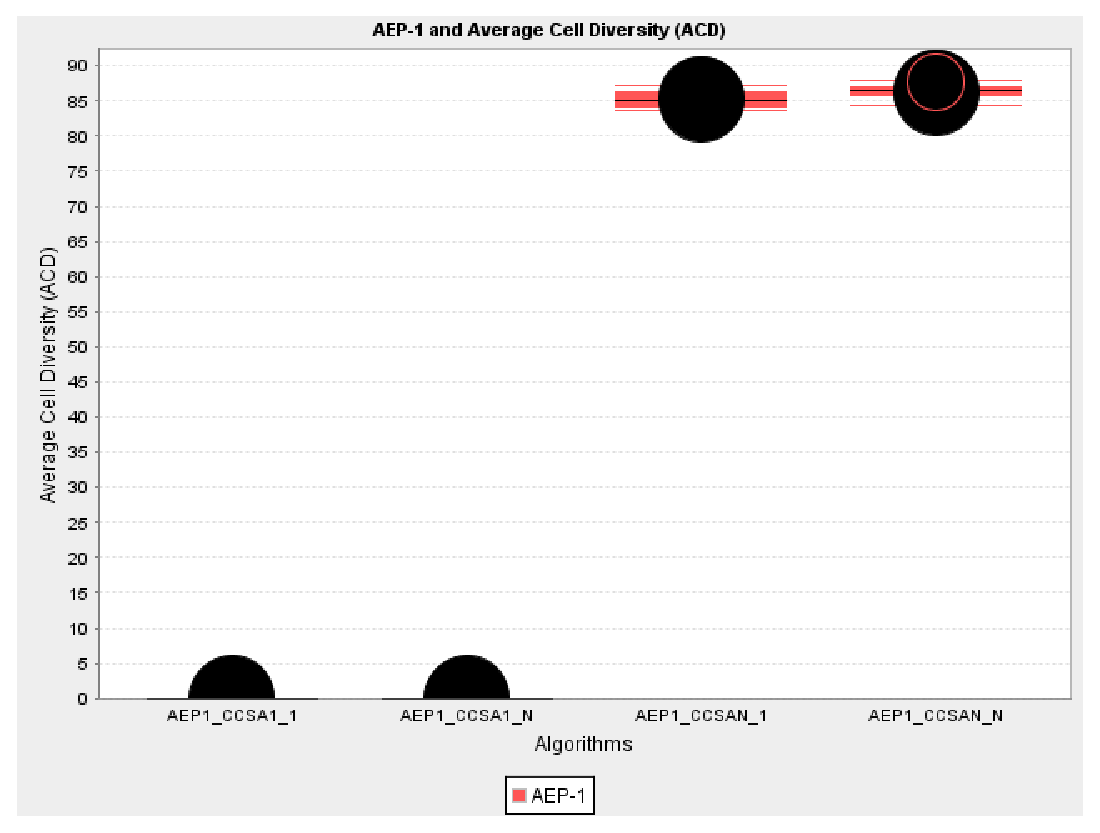
\includegraphics[scale=0.40]{Cells/CCSA-Study0-ACD}
	\end{minipage}}%
	%\hfill
	\subfloat[Average Cell Error (ACE) on ACSP-1.]{
	\label{fig:tissues:ccsa::study0:ace:boxplot} %% label 
	\begin{minipage}[t]{0.50\textwidth}
		\centering 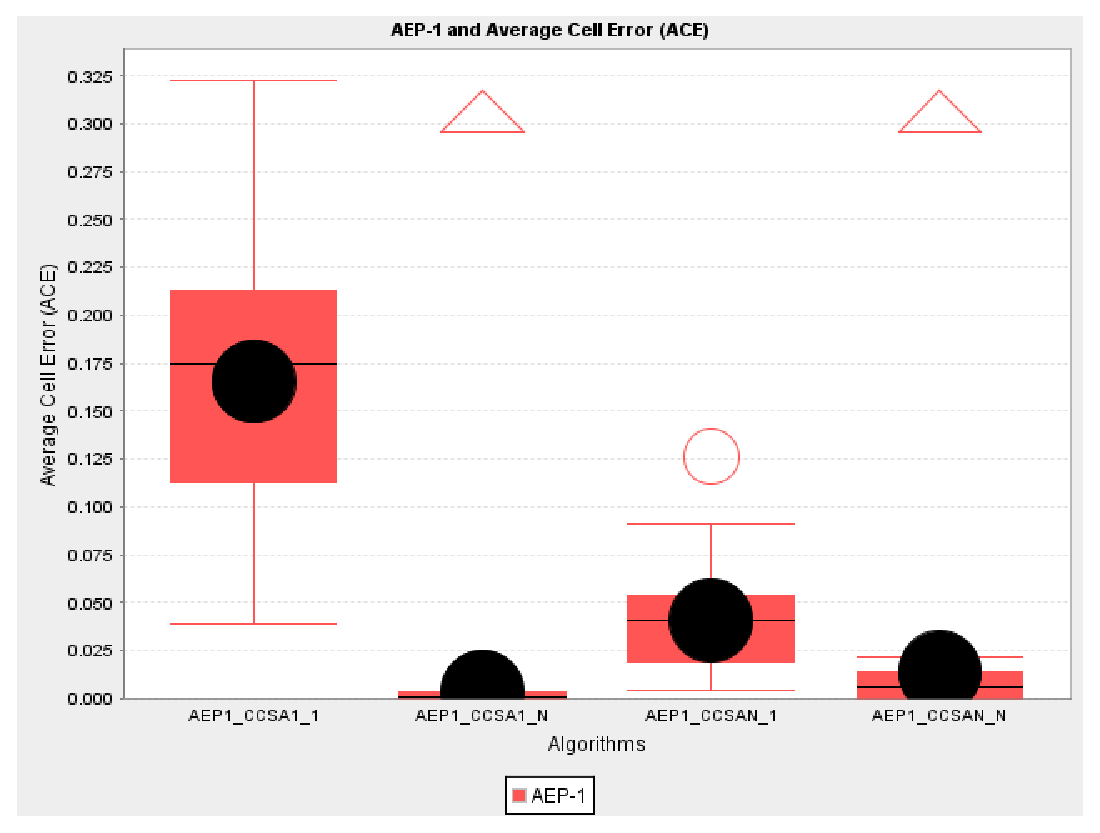
\includegraphics[scale=0.40]{Cells/CCSA-Study0-ACE}
	\end{minipage}}\\
	% new line for second set
	\subfloat[Average Cell Diversity (ACD) on ACSP-10.]{
	\label{fig:tissues:ccsa::study1:acd:boxplot} %% label 
	\begin{minipage}[t]{0.50\textwidth}
		\centering 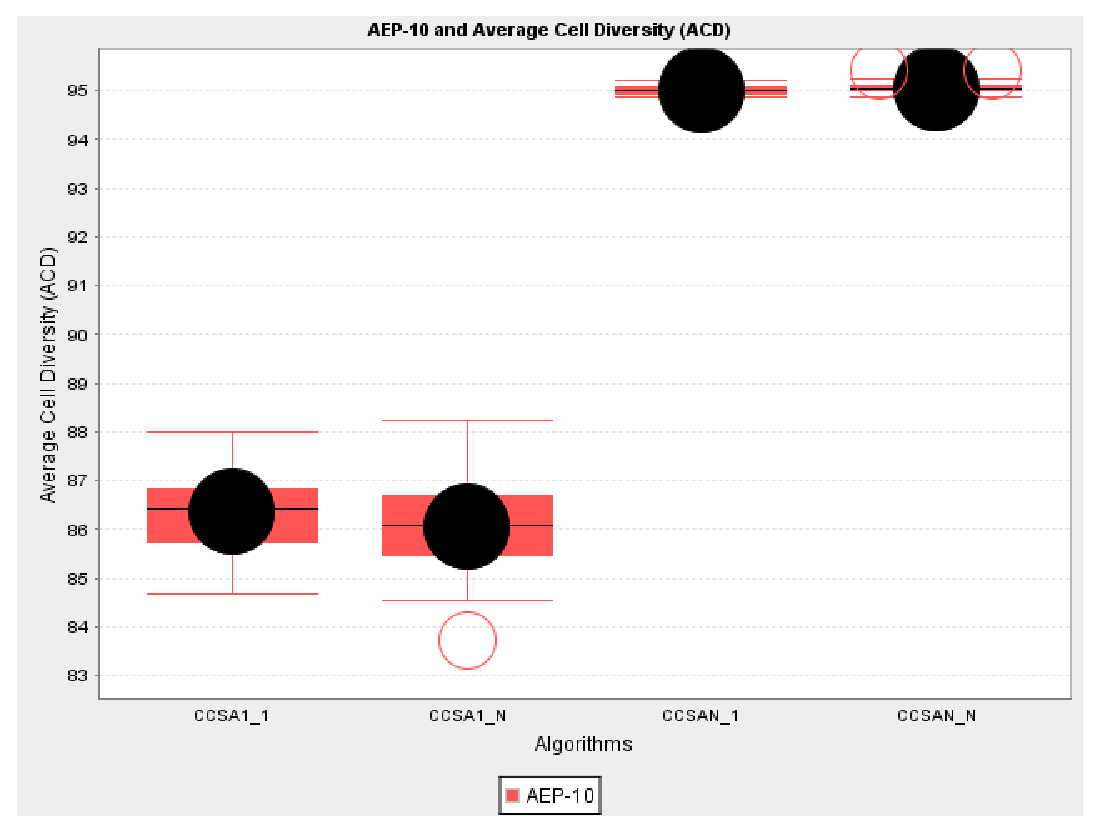
\includegraphics[scale=0.40]{Cells/CCSA-ACD}
	\end{minipage}}%
	%\hfill
	\subfloat[Average Cell Error (ACE) on ACSP-10.]{
	\label{fig:tissues:ccsa::study1:ace:boxplot} %% label 
	\begin{minipage}[t]{0.50\textwidth}
		\centering 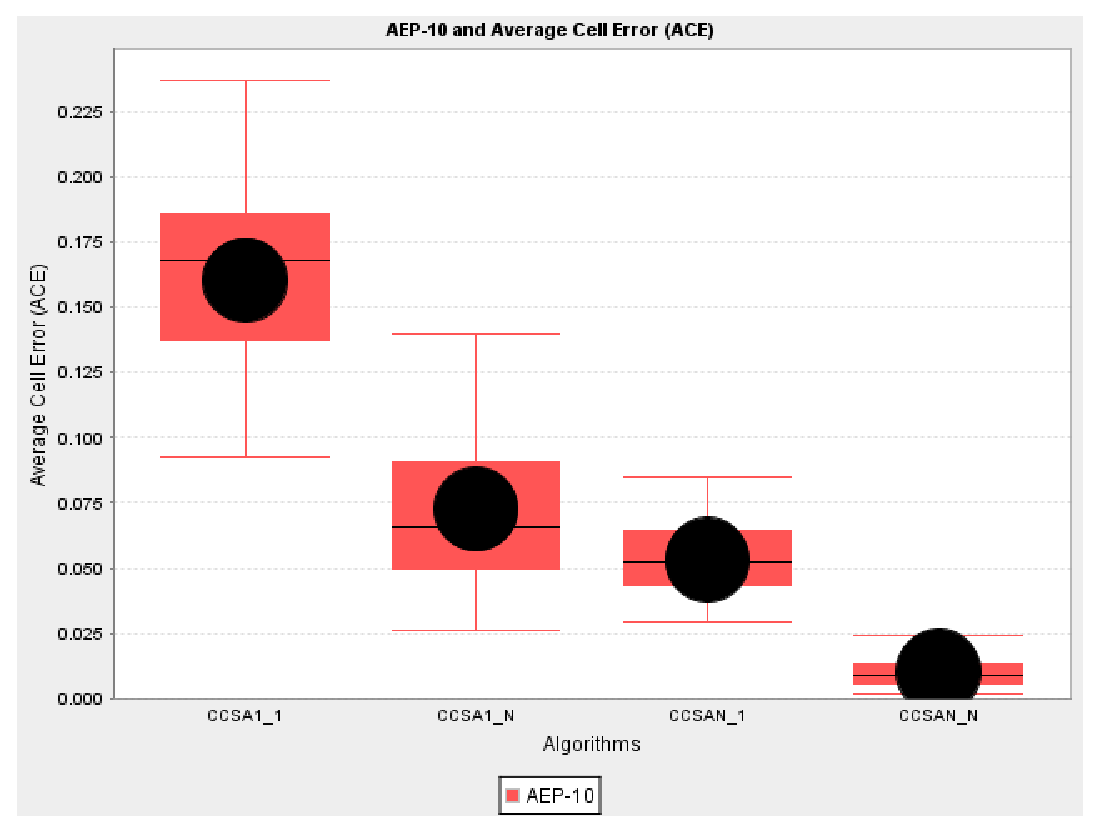
\includegraphics[scale=0.40]{Cells/CCSA-ACE}
	\end{minipage}}%
	\caption{Box-and-whisker plot's from the Cellular Empirical Study.}
	\label{fig:tissues:ccsa::study1:all:boxplot} %% label for entire figure
\end{figure}


% plots
\begin{figure}[htp]
	\subfloat[CCSA(N+N) on ACSP-1.]{
	\label{fig:cells:ccsa:acsp1:a} %% label 
	\begin{minipage}[t]{0.50\textwidth}
		\centering 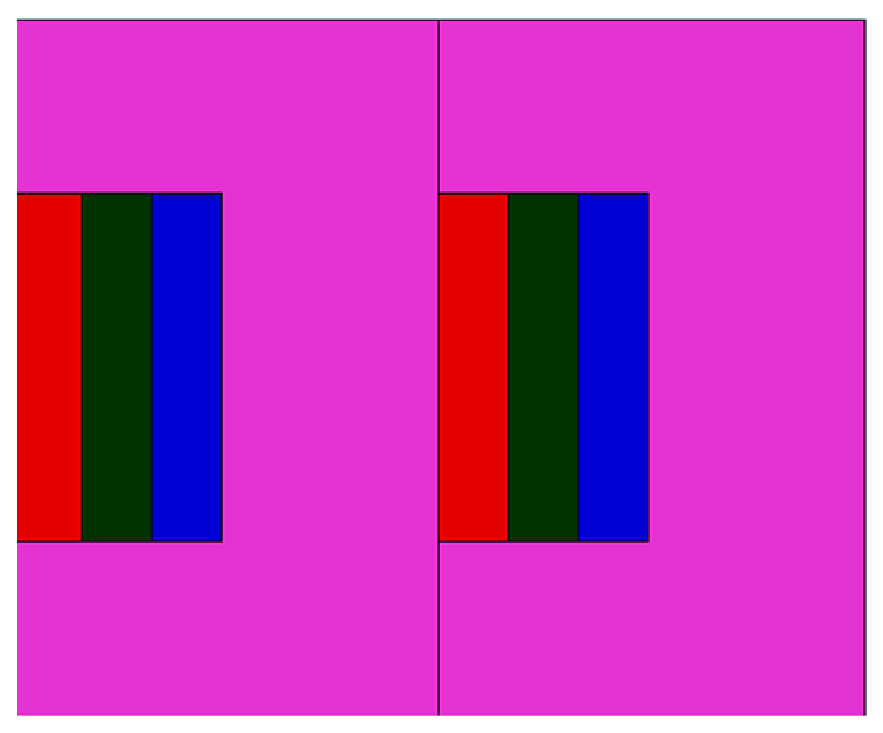
\includegraphics[scale=0.45]{Cells/CCSA(N+N)-ACSP-1}
	\end{minipage}}%
	\hfill
	\subfloat[CCSA(N+N) on ACSP-10.]{
	\label{fig:cells:ccsa:acsp10:b} %% label 
	\begin{minipage}[t]{0.50\textwidth}
		\centering 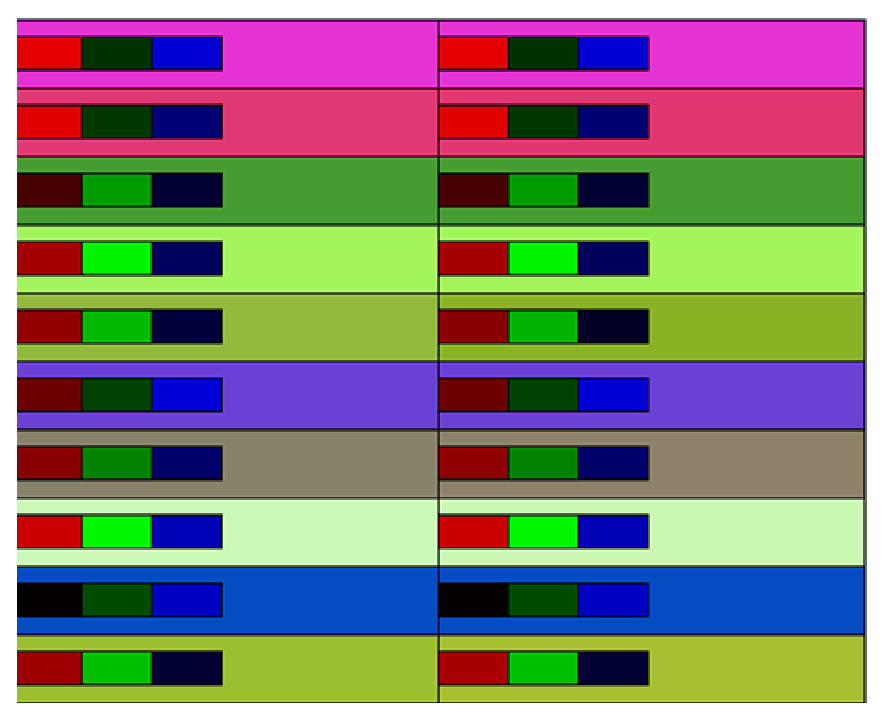
\includegraphics[scale=0.45]{Cells/CCSA(N+N)-ACSP-10}
	\end{minipage}}\\
	% end
	\caption{Example plots of $T_{rs}$ from the CCSA(N+N) at the end of the run on left section on both plots, for both ACSP-1 and ACSP-10, where the problem solution is represented on the right of each plot, and colour components within each CSP.}
	\label{fig:cells:ccsa:ccsa:plots} %% label for entire figure
\end{figure}


%
% Analysis
%
\subsubsection{Analysis}
This section provides an analysis of the results reported in the previous section in the context of the goals of the empirical study. Specifically, the analysis is broken down into the selection and clonal set size trends for small and large antigenic environments.

%
% Selection and Clonal Trends (ACSP-1)
% 
\paragraph{Selection and Clonal Trends (ACSP-1)}
% section
This section considers the selection and clonal trends of the CCSA configurations on ACSP-1.
% selection
The increase in the number of selected cells from 1 to $N$ resulted in a large increase in diversity as expected given the required shift in increase in the number of cells in the repertoire to support the increased selection size. The increase in the number of cells selected resulted in a decrease in error with a single clone and an increase when multiple clones were created.
% clone
The increase in the number of clones created for selected cells from 1 to $N$ resulted in very minor differences in the repertoire diversity, although did result in a large decrease in the average cell error.
% trends
The results confirmed the expectation that in the optimisation of a repertoire for a single antigen, the creation of more clones results in an improved system capability given that each clone represents a new trial and potential improvement over an already relatively good structure. 

%
% Selection and Clonal Trends (ACSP-10)
% 
\paragraph{Selection and Clonal Trends (ACSP-10)}
% section
This section considers the selection and clonal trends of the CCSA configurations on ACSP-10. 
% selection
The increase in the number of selected cells resulted in a decrease in the system error with a small repertoire, although in this case the trend held for both small and large repertoire sizes. 
% clone
The increase in the number of clones resulted in only very minor changes to the average cell diversity, although resulted in a consistent decrease in the the average cell error.
% trends
The increase in the size of the antigenic environment did not disrupt the general trend of increase number of clones resulting in increase system capability. Unlike the single antigen case, the increase in the number of selected cells also consistently resulted in a decrease in average cell error. 

%
% Conclusions
%
\subsubsection{Conclusions}
This section summarises the findings of the empirical study into the Cellular Clonal Selection Algorithm in terms of the primitives that were the focus of the study and the expectations that motivated the study.

\begin{enumerate}
		\item The Cellular Clonal Selection Algorithm successfully addressed 1 and 10 antigen problems, demonstrating itself as a viable realisation of a foundational clonal selection adaptive strategy under the circumstances considered.
		\item The increase in the number of selected cells (allocated resources) results in improved system capability with small cloning on the single antigen problem, although is consistently beneficial on the larger antigenic problem.
		\item The increase in the number of clones (trials) results in an improved system capability across the tested antigenic environments.	
\end{enumerate}


%
% Replacement Clonal Selection Empirical Study
%
\subsection{Replacement Empirical Study}
\label{sec:cells:ccsa:rcsa}

%
% Aim
%
\subsubsection{Aim}
The aim of this empirical study was to investigate the properties of the CCSA and the RCCSA as a viable realisation of cellular clonal selection that promote improved utilisation of repertoire resources. Improved utilisation will effect the composition and may effect the capabilities of a repertoire, where the promotion and maintenance of redundant perspectives is expected to provide benefits in terms of fault tolerance. Toward this end, the study had the following goals:

\begin{enumerate}
	\item Assess varied clonal integration mechanisms with CCSA that promote concurrent redundant perspectives of each antigen.
	\item Assess varied clonal integration mechanisms with RCCSA that promote concurrent perspectives and compare to CCSA.
\end{enumerate}

%
% Method
%
\subsubsection{Method}

%
% Problems
%
\paragraph{Problems}
This study used the ACSP-10 problem used for the CCSA empirical study in Section~\ref{sec:cells:ccsa:ccsa}.

% 
% Algorithms
%
\paragraph{Algorithms}
This section considers varied configurations of the CCSA and the RCCSA. The configuration parameters of each algorithm type are presented in Table~\ref{tab:cells:clonalselection:rccsa}. The chosen configurations of the repertoire, number of selected cells and number of clones facilitate the allocation of a maximum of six repertoire position per antigen.
% CCSA
The CCSA configurations included the CCSA(N+N) from CCSA empirical study in Section~\ref{sec:cells:ccsa:ccsa} as well as two extensions. CCSA(N+N)-G aggregates all clones into a single group which collectively compete with the $N_{selected}$ selected cells from the repertoire for their position. CCSA(N+N)-GS also aggregates all clones into a single clonal group, each of which competes with the same number of the best matching cells as there are in the clonal set drawn from the repertoire.
% RCSA
Two variations of the RCCSA algorithm (defined in Algorithm~\ref{alg:cells:realisation:algorithms:rccsa:exposure}) were assessed, both of which used Hamming Distance (Equation~\ref{eq:cells:realisation:hamming}) between cells in the replacement mechanism. The RCCSA-H configuration allowed clones to select the most similar cells in the repertoire to compete with for a position, whereas the RCCSA-H-ES configuration restricted selection to those cells in the repertoire that were not clonal siblings (hamming similarity excluding siblings). 

\begin{table}[htp]
	\centering\small
		\begin{tabular}{lllllll}
		\toprule
		\emph{CSA} & $N_{cells}$ & $N_{selected}$ & $N_{clones}$ & \emph{Clones ($A$)} & \emph{Positions} & \emph{Clones ($I$)} \\ 
		\toprule
		\emph{N+N} & 60 & 2 & 3 & 6 & 2 & 60 \\ 
		\emph{N+N-G} & 60 & 2 & 3 & 6 & 2 & 60 \\ 
		\emph{N+N-GS} & 60 & 2 & 3 & 6 & 6 & 60 \\ 
		\emph{RCCSA-H} & 60 & 2 & 3 & 6 & 6 & 60 \\ 
		\emph{RCCSA-H-ES} & 60 & 2 & 3 & 6 & 6 & 60 \\ 
		\bottomrule
		\end{tabular}
	\caption{Summary of the assessed configuration for the CCSA-RCCSA empirical study.}
	\label{tab:cells:clonalselection:rccsa}
\end{table}


%
% Experiment
%
\paragraph{Experiment}
This study used the same experimental configuration including stop conditions, measures, as were used for the CCSA empirical study in Section~\ref{sec:cells:ccsa:ccsa}. 
% ABMCPA
An additional measure was used to provide an assessment of the number of cells ($C$) in the repertoire ($T$) specialised to each antigen ($A$) in the scope of the problem ($I$). This measure is called the \emph{Average Best Matching Cells Per Antigen (ABMCPA)} defined in Equation~\ref{eq:cells:ccsa:rcca:abmcpa} that assessed and located the set of best matching cells for each antigen (Algorithm~\ref{alg:cells:ccsa:rccsa:bmc}) and averaged the number of cells returned for each antigen.

\begin{algorithm}[htp]
  \SetLine
  
  \SetKwData{Tissue}{T}
  \SetKwData{Antigen}{A}
  \SetKwFunction{Exposure}{Exposure}
  
  \KwIn{\Tissue, \Antigen}		
  \KwOut{$T_{BMC}$}
  
	$T_{BMC} \leftarrow$0\;
	\For{$C_i \in$ \Tissue}
	{
		\Exposure{\Antigen, $C_i$}\;
		% check for new set
		\uIf{${T_{BMC}}_n > 0$}
		{
			$C\prime \leftarrow {T_{BMC}}_i$\;
			\uIf{$C_i$.affinity $<$ $C\prime$.affinity}
			{
				% clear
				$T_{BMC} \leftarrow$0\;
				$T_{BMC} \leftarrow C_i$\;
			}
			\ElseIf{$C_i$.affinity $\equiv$ $C\prime$.affinity}
			{
				$T_{BMC} \leftarrow C_i$\;
			}
		}
		\Else
		{
			$T_{BMC} \leftarrow C_i$\;
		}		
	}
	\Return{$T_{BMC}$}\;
	
	\caption{Best Matching Cells (BMC's) for a given Antigen.}
	\label{alg:cells:ccsa:rccsa:bmc}	
\end{algorithm}



\begin{equation}
	AverageBMCPerAntigen(I,T) = \frac{1}{I_n} \sum_{i=1}^{I_n} {ABMCS(A_i, T)}_n
	\label{eq:cells:ccsa:rcca:abmcpa}
\end{equation}


%
% Results
%
\subsubsection{Results}
% tables
Table~\ref{tab:cells:ccsa:rccsa} provides a summary of results for each algorithm-problem combination including the mean ($\bar{x}$) and standard deviation ($\sigma$) of collected measure values. The non-parametric Mann-Whitney~U statistical test was calculated pair-wise for all algorithms. 
% figures
Figures \ref{fig:tissues:ccsa:rccsa:acd:boxplot}, \ref{fig:tissues:ccsa:rccsa:ace:boxplot}, and \ref{fig:tissues:ccsa:rccsa:abmca:boxplot} show the ACD, ACE, and ABMCPA on all algorithms respectively. 
% plots
Figure~\ref{fig:cells:ccsa:rccsa:plots} provides example plots of the state of the repertoire (left of each plot) compared to the problem domain (right of each plot) from each of the five algorithms (same configuration, random seeds of 1 and 5 for the algorithm and problem respectively). 

\begin{table}[htp]
	\centering\small
		\begin{minipage}{0.80\textwidth}		
		  \centering
			\begin{tabular}{llllllll}			
			\toprule
			\textbf{Problem} & \textbf{System} & \multicolumn{2}{c}{\textbf{ACD}} & \multicolumn{2}{c}{\textbf{ACE}} & \multicolumn{2}{c}{\textbf{ABMCPA}}\\
			\midrule
			\emph{ACSP} & \emph{CSA} & $\bar{x}$ & $\sigma$ & $\bar{x}$ & $\sigma$ & $\bar{x}$ & $\sigma$\\
			\toprule
			ACSP-10 & CCSA(N+N) & 94.356 & 0.171 & 0.027 & 0.012 & 1 & 0 \\
			ACSP-10 & CCSA(N+N)-G & 93.995 & 0.24 & 0.023 & 0.014 & 1.82 & 0.124 \\
			ACSP-10 & CCSA(N+N)-GS & 88.456 & 0.937 & 0.062 & 0.015 & 4.907 & 0.528 \\
			ACSP-10 & RCCSA-H & 94.37 & 0.18 & 0.03 & 0.013 & 1 & 0 \\
			ACSP-10 & RCCSA-H-ES & 88.083 & 0.79 & 0.028 & 0.013 & 2.653 & 0.385 \\
			\multicolumn{2}{l}{\emph{Significant}} & True\footnote{False for CCSA(N+N) and RCCSA-H} &  & True &  & True\footnote{False for CCSA(N+N) and RCCSA-H} & \\
			\bottomrule
			\end{tabular}			
		\end{minipage}
	\caption{Summary of results from the CCSA-RCCSA empirical study on ACSP-10.}
	\label{tab:cells:ccsa:rccsa}
\end{table}

\begin{figure}[htp]
	\subfloat[Average Cell Diversity (ACD) on ACSP-10.]{
	\label{fig:tissues:ccsa:rccsa:acd:boxplot} %% label 
	\begin{minipage}[t]{0.50\textwidth}
		\centering 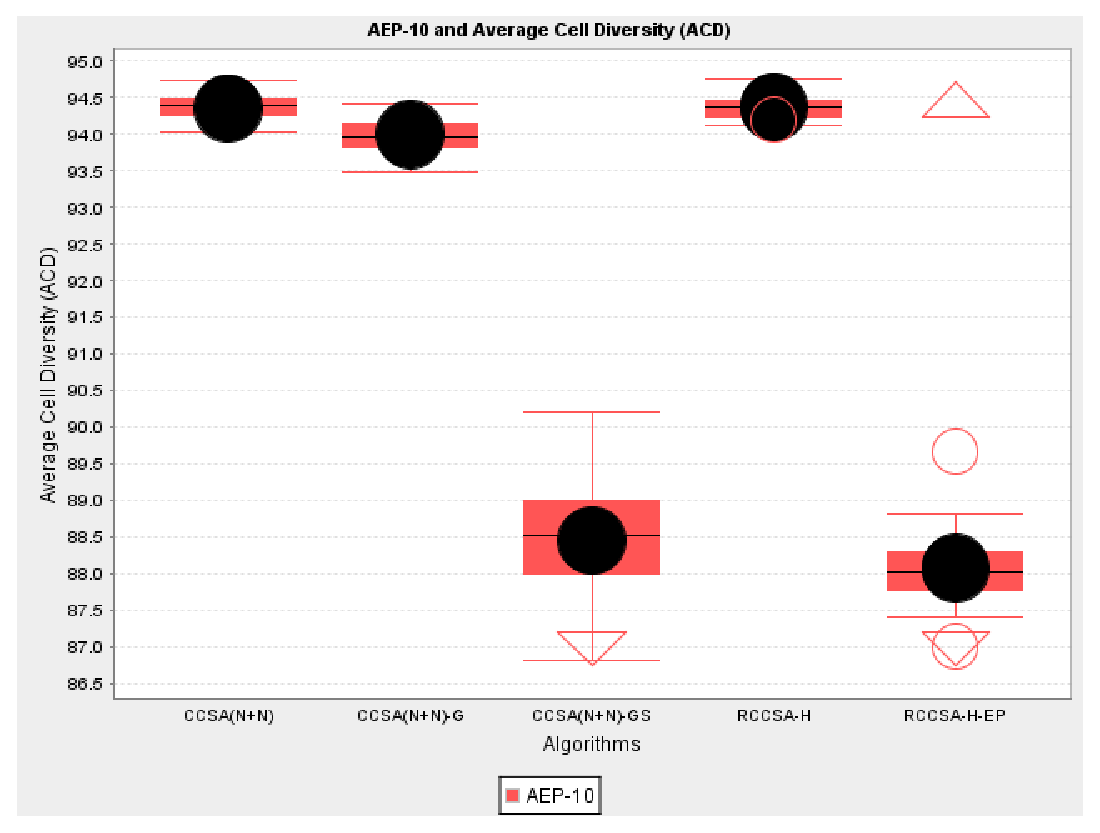
\includegraphics[scale=0.40]{Cells/CCSA-Study2-ACD}
	\end{minipage}}%
	\hfill
	\subfloat[Average Cell Error (ACE) on ACSP-10.]{
	\label{fig:tissues:ccsa:rccsa:ace:boxplot} %% label 
	\begin{minipage}[t]{0.50\textwidth}
		\centering 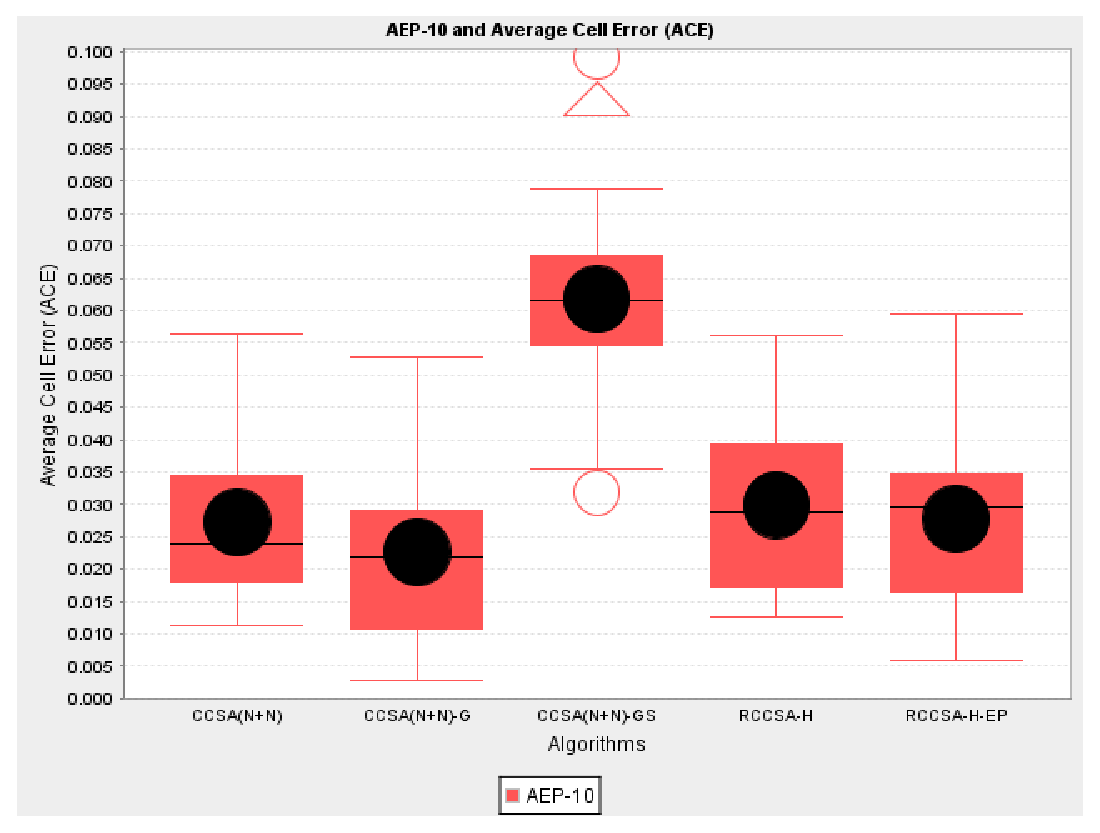
\includegraphics[scale=0.40]{Cells/CCSA-Study2-ACE}
	\end{minipage}}\\
	%\hfill
	\subfloat[Average BMC Per Antigen (ABMCPA) on ACSP-10.]{
	\label{fig:tissues:ccsa:rccsa:abmca:boxplot} %% label 
	\begin{minipage}[t]{\textwidth}
		\centering 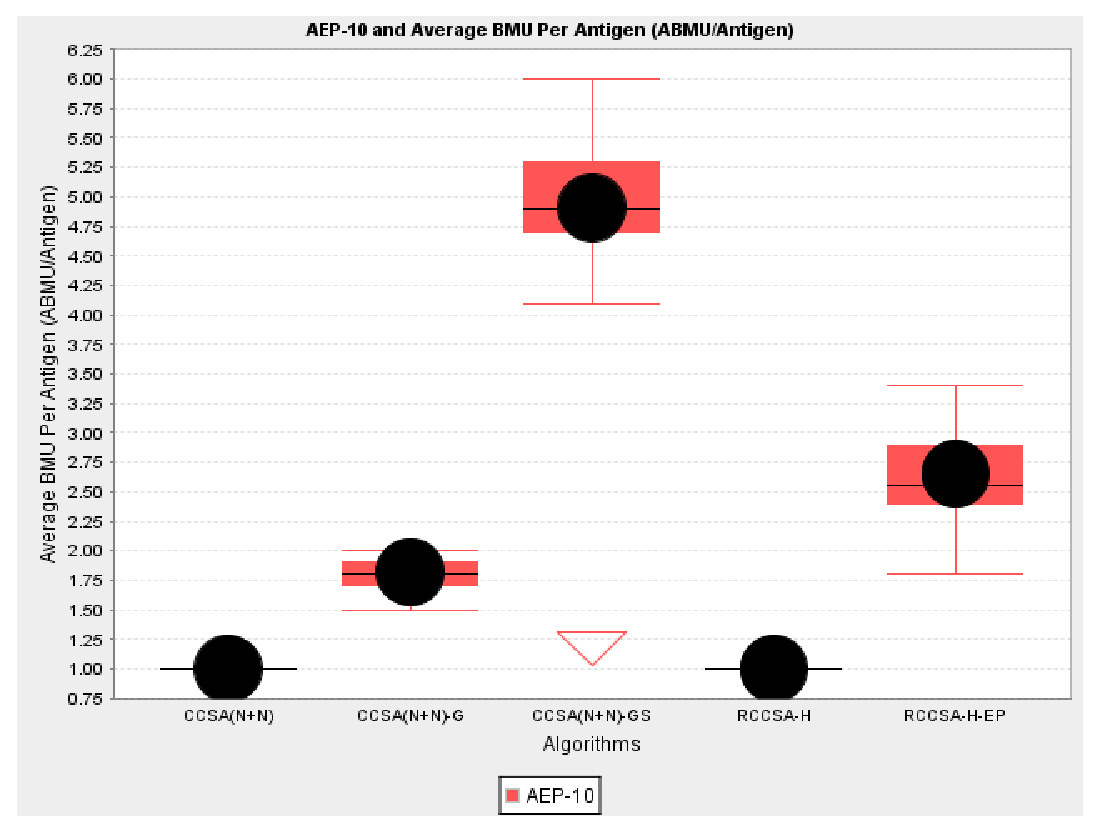
\includegraphics[scale=0.40]{Cells/CCSA-Study2-ABMCA}
	\end{minipage}}%
	\caption{Box-and-whisker plot's from the Replacement Empirical Study.}
	\label{fig:tissues:rccsa::study2:all:boxplot} %% label for entire figure
\end{figure}

% plots
\begin{figure}[htp]
	\subfloat[CCSA(N+N).]{
	\label{fig:cells:ccsa:rccsa:a} %% label 
	\begin{minipage}[t]{0.50\textwidth}
		\centering 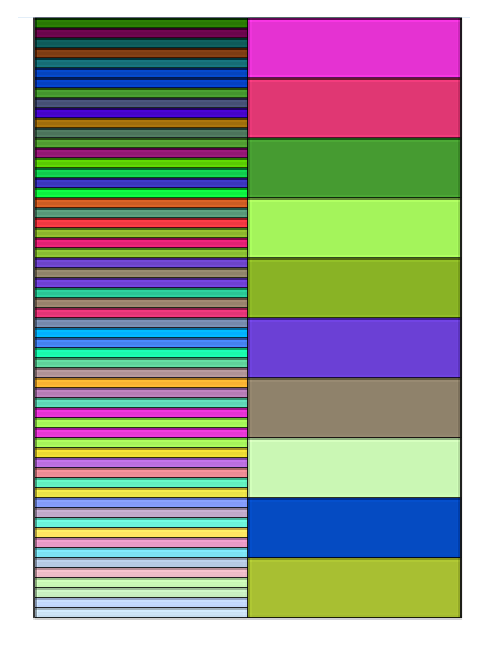
\includegraphics[scale=0.45]{Cells/CCSA(N+N)-plot}
	\end{minipage}}%
	\hfill
	\subfloat[(N+N)-G.]{
	\label{fig:cells:ccsa:rccsa:b} %% label 
	\begin{minipage}[t]{0.50\textwidth}
		\centering 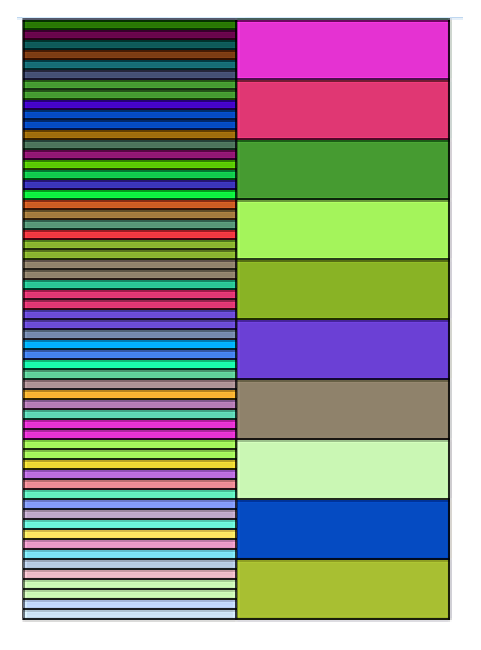
\includegraphics[scale=0.45]{Cells/CCSA(N+N)-G-plot}
	\end{minipage}}\\
	% new line for second set	
	\subfloat[(N+N)-GS.]{
	\label{fig:cells:ccsa:rccsa:c} %% label 
	\begin{minipage}[t]{0.50\textwidth}
		\centering 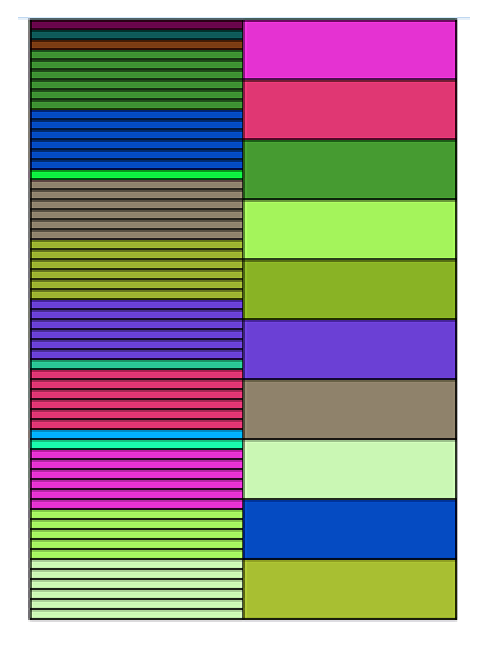
\includegraphics[scale=0.45]{Cells/CCSA(N+N)-GS-plot}
	\end{minipage}}%
	\hfill
	\subfloat[RCCSA-H.]{
	\label{fig:cells:ccsa:rccsa:d} %% label 
	\begin{minipage}[t]{0.50\textwidth}
		\centering 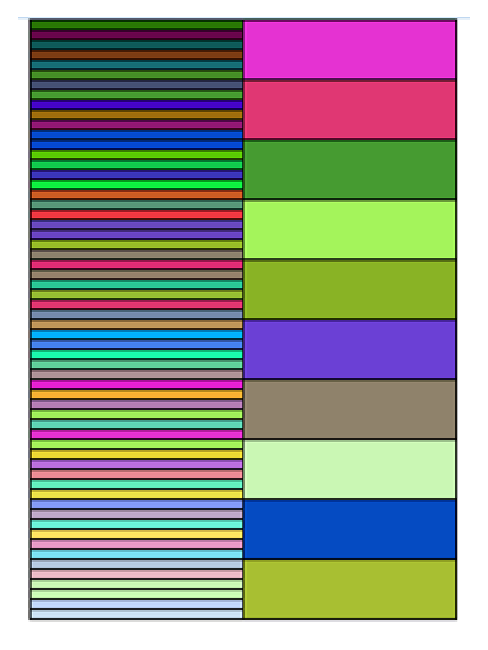
\includegraphics[scale=0.45]{Cells/RCCSA-H-plot}
	\end{minipage}}\\
	% new line for third set	
	\subfloat[RCCSA-H-ES.]{
	\label{fig:cells:ccsa:rccsa:e} %% label 
	\begin{minipage}[t]{\textwidth}
		\centering 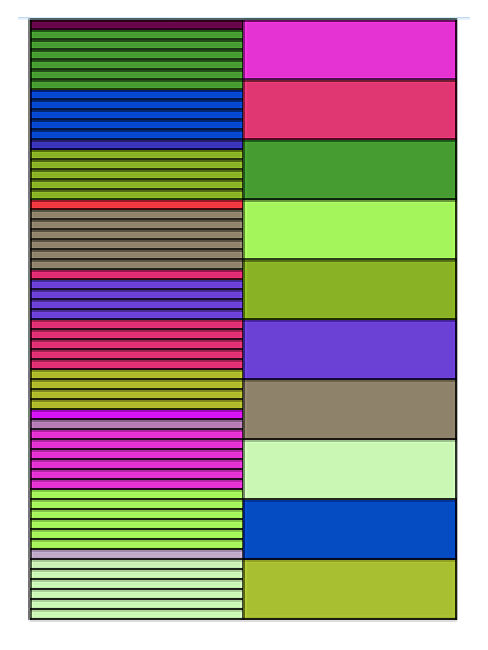
\includegraphics[scale=0.45]{Cells/RCCSA-H-ES-plot}
	\end{minipage}}	
	% end
	\caption{Plots of the ordered state of the repertoire after the triggering of the stop condition (left of each plot) for the assessed CCSA and RCCSA algorithms on the ACSP-10, where the right of each plot provides the problem optima.}
	\label{fig:cells:ccsa:rccsa:plots} %% label for entire figure
\end{figure}


%
% Analysis
%
\subsubsection{Analysis}
This section provides an analysis of the results reported in the previous section in the context of the goals of the empirical study. 

%
% CCSA Trends
%
\paragraph{CCSA Trends}
% section
% This section considers the behaviour trends of the CCSA and varied replacement mechanisms. 
% diversity
With regard to average cell diversity, the aggregation and thus competition between the entire clonal set with the selected set resulted in a slight drop in diversity, although the relaxing of the competition from progenitor cells to the entire repertoire resulted in a further larger decrease in diversity by $\approx 5.5$ bits.
% error
Interestingly the CCSA(N+N)-G achieved a slightly lower error than CCSA(N+N) where the further relaxation of competition in CCSA(N+N)-GS resulted in a large relative increase in the ACE.
% bmu 
Correlating with the decrease in ACD, the relaxation in the integration of the clones resulted in an increase in the number of best matching cells (BMC's) per antigen, rising to an average of $\approx 5$ in the case of CCSA(N+N)-GS.
% trends
The results demonstrate that multiple concurrent and redundant perspectives of antigen can be achieved by relaxing the replacement competition in CCSA which decreases repertoire diversity. The results also highlight that competition between the clonal set results in an improved result in terms of ACE and ABMCPA over CCSA(N+N), although the relaxation from progenitor set to whole repertoire dramatically increases ABMCPA at expense of increasing the systems general capability. The specialisation of each antigen's cellular imprint in the repertoire provided by CCSA(N+N)-GS is clearly demonstrated in Figure~\ref{fig:cells:ccsa:rccsa:c} compared to CCSA(N+N)-G in Figure~\ref{fig:cells:ccsa:rccsa:b}.

%
% RCCSA Trends
%
\paragraph{RCCSA Trends}
% section
% This section considers the behaviour trends of the RCCSA and the two replacement mechanisms. 
% diversity
The exclusion of clonal siblings from replacement resulted in a significant decrease in diversity, the same seen between CCSA(N+N)-G and CCSA(N+N)-GS. 
% error
The exclusion of progeny also resulted in a very slight decrease in ACE over RCCSA-H.
% bmu
Interestingly, the repertoire-wide competition between the aggregated clonal set in RCCSA-H resulted in a single average BMC per antigen, whereas, the exclusion of progeny during replacement promoted the competition between the concurrent clonal set such that ABMCPA increased to $\approx 2.5$.
% trends
Also interesting was that the ACE and ABMCPA results for RCCSA-H were not significantly different from CCSA(N+N), demonstrating that unrestricted similarity-affinity based replacement into the repertoire behaves much like CCSA(N+N) confirming the expectation that motivated the exclusion of clonal progeny: that they are more similar. Also interesting is that the increase in ABMCPA with RCCSA-H-ES also resulted in a relative increase in ACE compared to CCSA(N+N) and CCSA(N+N)-G, suggesting that for the mechanisms used, increasing the specialisation of the cellular footprint for each antigen comes at the expense of general repertoire competence. 

%
% Conclusions
%
\subsubsection{Conclusions}
This section summarises the findings of the empirical study into the CCSA and RCCSA in terms of the primitives that were the focus of the study and the expectations regarding proportional resource allocation.

\begin{enumerate}
		\item Relaxing the constraints for competition in the integration clones into the repertoire results in increased number of concurrent redundant perspectives of an antigen in the repertoire for CCSA and RCCSA.
		\item Strong inter-clonal competition in CCSA results in improved performance with a slight increase in size in the number of redundant perspectives.
		\item Repertoire-wide integration restrained by only similarity-and-affinity in RCCSA approximates CCSA(N+N) in behaviour.
		\item Repertoire-wide integration restrained by affinity in CCSA or by similarity-and-affinity-exclusion in RCCSA results in a large increase in the size and quality of the number of redundant perspectives at the cost of general repertoire capability under both algorithms. 		
\end{enumerate}

%
% Degenerate Clonal Selection Empirical Study
%
\subsection{Degenerate Empirical Study}
\label{sec:cells:ccsa:dcsa}
There is a lack of a one-to-one correspondence between antigen and receptors in the acquired immune system. A given antigen may have the capacity to trigger a very larger number of receptors, therefore resulting in a polyclonal activation, although a response is typically oligoclonal. This may be accounted for by the competition between clones for selection by the antigen. In addition, a given receptor may respond to a large number of antigens, thus resulting in a polyclonal response, something that cannot be accounted for by the clonal selection theory. In the Cognitive Theory of Immunology, Cohen refer to this polyclonal response of a given receptor as \emph{cellular degeneracy}, where those receptors that are without a context are cross-specific, including auto-specific \cite{Cohen2004}. A polyclonal response is the antithesis of clonal dominance (a feature that underlies the clonal selection theory). The solution as proposed in cognitive theory is that specificity is an emergent phenomenon \cite{Cohen2001, Hershberg2003}. Unlike the clonal selection theory, where specificity is a property of antigen-receptor interaction, emergent specificity is a down-stream effect that occurs after the initial interaction. A collection of varied and communicating cell types respond to the antigen in context. This is the so-called meta-response of cognitive theory, called the co-response or corespondence. The degeneracy of cell signalling is proposed as the basis of plasticity both in the brain and in the immune system, and is the feature exploited by antibiotics and pharmaceuticals.

\begin{figure}[htp]
	\centering
	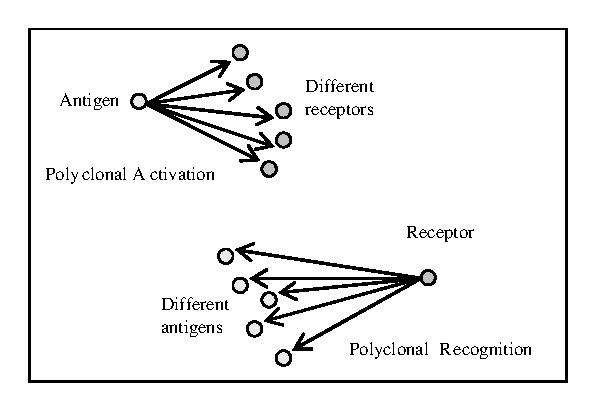
\includegraphics[scale=0.85]{ClonalSelection/cognitive-polyclonal}
	\caption{Depiction of a polyclonal activation and a polyclonal response.}
	\label{pic:cognitive:polyclonal}
\end{figure}

% general properties i care about
Clonal selection accounts for the restriction of a potential polyclonal activation of the repertoire to an oligoclonal activation by dominant clones out competing the less well fitted clones (referred to as clonal dominance). The classical theory does not account for lack of one-to-one correspondence between cells and antigen (the cross-reactivity of receptors referred to as polyclonal response). Cognitive immune theory accounts for polyclonal response between antigen and receptors by suggesting (1) that cells in isolation are degenerate and cross-specific, (2) context defines the use for degenerate cells resulting in emergent specificity.

%
% Aim
%
\subsubsection{Aim}
Section~\ref{sec:cells:realised:trends} considered the expectations of clonal selection on a degenerate repertoire, specifically with regard to the pressures required to facilitate polyclonal activation and response. The aim of this empirical study is to investigate these expectations in the context of cellular clonal selection. 
% goals
Toward this end, the study had the following goals:

\begin{enumerate}	
	\item Investigate a clonal selection with a degenerate representation.
	\item Assess selective pressures and explicit aggregation to constrain polyclonal activation and response.	
\end{enumerate}

%
% Method
%
\subsubsection{Method}

%
% Problems
%
\paragraph{Problems}
% analogy
The definition of the Colour Space Domain in Section~\ref{subsec:cells:paradigm:colourspace} highlighted a `retina and colour perception' analogy made by Cohen to describe cellular degeneracy and emergent specificity. The problems in this section are motived by that analogy.
% same things
This study used the ACSP-10 problem used for the CCSA empirical study in Section~\ref{sec:cells:ccsa:ccsa}, although evaluated on a per colour component basis. To differentiate this mode of evaluation from the holistic ACSP, it is referred to as the Determinant Colour Space Problem (DCSP-10).
% Components
A degenerate colour representation was used called component degeneracy where each colour was divided into the its Red, Green, and Blue components. Components are denoted $D$, where a $A = \{D_1, D_2, D_3\}$ for each colour space pattern. Degenerate component cells were assessed using Equation~\ref{eq:cells:realised:component:distance}, where each degenerate component cell was defined by a 64-bit bitstring and decoded to a real value using Gray Code (Equation~\ref{eq:cells:realised:graycode}). Components were considered a symbolic degenerate representation as each component has direct meaning via their linear aggregation in the the context of a colour space pattern.

% Component Distance
\begin{equation}
	ComponentDistance(D, C) = \left| D - C \right|
	\label{eq:cells:realised:component:distance}
\end{equation}

% 
% Algorithms
%
\paragraph{Algorithms}
The study considers a \emph{Degenerate Cellular Clonal Selection Algorithm (DCCSA)} as an extension of the RCCSA (defined in Algorithm~\ref{alg:cells:realisation:algorithms:rccsa:exposure}) that uses a degenerate representation. RCCSA was selected as a base algorithm because (1) it achieves adequate results in terms of repertoire capability, and (2) because it achieves multiple high-affinity concurrent perspectives (proportional repertoire composition) on antigen to which it is exposed.
% component
The RCCSA was configured with the following configuration: $N_{cells}=100$, with $N_{selected}=3$, and $N_{clones}=1$ per determinant exposure, resulting in a resource allocation of three cells per component, or nine cells per antigen. A Hamming-based similarity assessment was used in replacement, with clonal sibling exclusion. Two variations of the degenerate cellular component selection were considered as follows: (1) explicit per-component selection called DCCSA-E, and (2) pre-committed component cells called DCCSA-P. Both approaches aggregated the best degenerate cell for each component into a holistic solution to address each given antigen in the ACSP. Explicit per-component selection maintained a repertoire of uncommitted components that were assessed and selected in the context of each component of each colour space pattern. This allowed degenerate cell reuse across the components of a single antigen and across the components of multiple antigen. Pre-committed component cells involved the management of one sub-repertoire for each component, where the size of each repertoire was a fraction of the total number of cells ($\lfloor \frac{1}{N_{components}} \times N_{cells}\rfloor$). 


%
% Experiment
%
\paragraph{Experiment}
% same things
This study used the same experimental configuration including stop conditions, measures, as were used for the CCSA empirical study in Section~\ref{sec:cells:ccsa:ccsa}. 
% component
An additional measure was introduced for the degenerate component algorithms that assessed the extent of the cross-reactivity of the repertoire called the \emph{Average Polyclonal Response Error (APRE)}, defined in Equation~\ref{eq:cells:ccsa:dccsa:apre}. APRE provides an indication of the average repertoire error per component. 
% APRE
\begin{equation}
	% across all antigen
	APRE(I, T) = \frac{1}{I_n \times {A_i}_n} \sum_{i=1}^{I_n}
	% across all components
	\left(\sum_{j=1}^{{A_i}_n}
	% across the entire repertoire
	\left(\frac{1}{T_n} \sum_{k=1}^{T_n}
	% component distance
	ComponentDistance({A_i}_j, C_k)	
	\right)\right)
	\label{eq:cells:ccsa:dccsa:apre}
\end{equation}


%
% Results
%
\subsubsection{Results}
% tables
Table~\ref{tab:cells:ccsa:dccsa} provides a summary of results for each algorithm-problem combination including the mean ($\bar{x}$) and standard deviation ($\sigma$) of collected measure values. The non-parametric Mann-Whitney~U statistical test was calculated pair-wise for all algorithms. 
% figures
%Figure~\ref{fig:tissues:ccsa:dcccsa:ace:boxplot} shows the ACS on both algorithms. 

\begin{table}[htp]
	\centering\small
		\begin{tabular}{llllllll}
		\toprule
		\textbf{Problem} & \textbf{System} & \multicolumn{2}{c}{\textbf{ACD}} & \multicolumn{2}{c}{\textbf{ACE}} & \multicolumn{2}{c}{\textbf{APRE}}\\
		\midrule
		\emph{AEP} & \emph{CSA} & $\bar{x}$ & $\sigma$ & $\bar{x}$ & $\sigma$ & $\bar{x}$ & $\sigma$\\
		\toprule
		DCSP-10 & DCCSA-E & 31.638 & 0.047 & 0.003 & 0.001 & 0.333 & 0.018 \\
		DCSP-10 & DCCSA-P & 31.627 & 0.059 & 0.008 & 0.003 & 0.334 & 0.019 \\
		\multicolumn{2}{l}{\emph{Significant}} & False &  & True &  & False & \\
		\bottomrule
		\end{tabular}
	\caption{Summary of results from the DCCSA empirical study on DCSP-10.}
	\label{tab:cells:ccsa:dccsa}
\end{table}

%\begin{figure}[htp]
%	\centering
%		\includegraphics[scale=0.35]{Cells/DCCCSA-ACE}
%	\caption{Box-and-whisker plot of Average Cell Error (ACE) on DCSP-10.}
%	\label{fig:tissues:ccsa:dcccsa:ace:boxplot}
%\end{figure}

%
% Analysis
%
\subsubsection{Analysis}
This section provides an analysis of the results reported in the previous section in the context of the goals of the empirical study, specifically (1) restrictive selection, and (2) explicit aggregation. 

%
% Restrictive Selection
%
\paragraph{Restrictive Selection}
The results showed little significant difference on the selected measures between the explicit and pre-committed selection mechanisms, other than a slightly improved cell error for the explicit approach. The strong similarity in results, in particular the Average Polyclonal Response Error demonstrate that the degenerate component clonal selection was generally unaffected when the repertoire was split into sub-repertoires per component compared to an integrated cross-component competitive repertoire. The minimum Hamming distance between generated colour space patterns likely resulted in little cross-colour space pattern reuse given the per-pattern/per-component specialisation of the repertoire, and the lack of difference between segregated and integrated component repertoires.
% pervasive polyclonal activation
An important consideration is that CCSA and RCCAS implicitly rely on restrictive selection to bound polyclonal activation of cells. This is clear if we consider a principle of cellular clonal selection that the scope of the repertoire available allowing $N_{cells}$ interactions (assessments and activations). Without constrained selection, the scope of repertoire would respond in its entirety each antigen exposure.

%
% Explicit Aggregation
%
\paragraph{Explicit Aggregation}
The clonal selection strategy by-design continues regardless of the integration of the product of exposure events. With respect to the problem domain, aggregation of the product of exposures is the critical concern of a degenerate representation. The chosen degenerate component representation was chosen because of its easy linear aggregation of the best matching components, always resulting in feasible aggregated responses at the per-$D$, per-$A$, and per-$I$ levels.
% sub-symbolic
One may consider a sub-symbolic representation for the ACSP that does not easily aggregate into holistic colour space patterns solutions, such as sub-bitstrings. This is an important example because it highlights that such representation does not hinder the clonal selection strategy. Degenerate sub-strings may be assessed based on hamming distances from exposed $A$'s or $D$'s providing enough information for selection, cloning and integration. The explicit aggregation of sub-strings is less natural than the component case, requiring perhaps a per-bit position frequency assessment and a deterministic or probabilist generation of a viable holistic solution at the $A$ scale. The example highlights that explicit aggregation may be suitable for the linear aggregation of components, although becomes more difficult with sub-symbolic representations one which clonal selection can still operate effectively. 
% pervasive degeneracy
Explicit aggregation also highlights that this problem-centric concern is scale independent, where the components of a colour, and the colours of a colour set are the linear aggregation of selected information which may or may not be the case for more elaborate applications.

%
% Conclusions
%
\subsubsection{Conclusions}
This section summarises the findings of the empirical study into the DCCSA in terms of the primitives that were the focus of the study and the expectations regarding proportional resource allocation.

\begin{enumerate}
	% primitives
	\item \emph{Degenerate Components}
	\begin{enumerate}
		\item Clonal Selection on components provides a viable realisation of cellular degeneracy under the circumstances considered where strong selection and aggregation can constrain polyclonal activation.
		\item A RCCSA results in little difference in the partitioning or aggregation of the repertoire and thus competition of degenerate cells, suggesting clonal independence promoted via replacement is sufficient for non-overlapping clonal specialisation (assuming a large enough repertoire).
		\item Explicit aggregation provides a context in which to bound polyclonal response to strongly activated (selected) structures.
	\end{enumerate}
	
	% findings
	\item \emph{Selection and Aggregation}
	\begin{enumerate}
		\item Strong selection is required in all cellular clonal selection algorithms to manage the implicit polyclonal activation that occurs as a result of each antigens interaction with the entire repertoire.
		\item Aggregation is independent of the principle clonal selection operations, requiring explicit integration into the process (for those applications that operate on sub-solution structures).
	\end{enumerate}
	
\end{enumerate}


%
% Spatial Repertoire
%
\section{Spatial Repertoire}
\label{sec:cells:spatial}
This section considers a spatial context as a method for forming relationships between units undergoing clonal selection and expansion. A spatial clonal selection paradigm is investigated which outlines a fixed lattice structured repertoire on which clonal selection operators are applied. 

%
% Spatial Clonal Selection
%
\subsection{Spatial Clonal Selection}
% metaphor
The processes of selection and maturation of lymphocytes occurs in the spatially distributed confines of the host organism lymphatic system \cite{Anderson1990a}. Further, the spatial organisation may be required to provide context to guide emergent specificity \cite{Cohen2001a}. 
% abstraction
The competition in the clonal selection principle is between cells for resources in the repertoire. Competition can be facilitated through differential selection of an activated set which results in differential allocation of resources for clones from the activated set. In envisaging the repertoire as a spatial structure, an additional level of competition is introduced called \emph{spatial competition}. This competition puts pressure on cells in the same spatial neighbourhood to compete with each other. This pressure may be used for either the activation of cells during \emph{selection} or \emph{replacement} by clones of activated cells. A simple one or two-dimensional lattice structure may be used in which receptors occupy grid positions of the lattice, and the ends of the structure wrap around (ring or toroid), removing edge effects. The structure may be an equally arbitrary number of dimensions, although low dimensionality facilitates visualisation. Such a spatial repertoire structure provides a manifestation of the space complexity limits imposed on repertoire size, and imposes relationships between arbitrary neighbouring receptors for a given antigenic stimulus. 

\begin{figure}[ht]
	\centering
	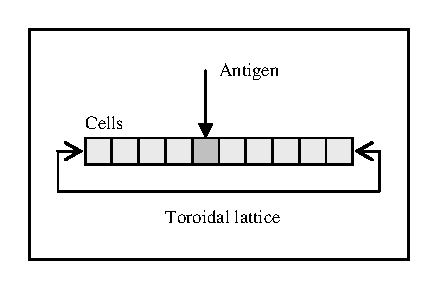
\includegraphics[scale=0.85]{Cells/cells-spatial-oned-lattice}
	\caption{Depiction of a one-dimensional toroidal lattice.}
	\label{pic:cells:spatial:lattice}
\end{figure}

%
% Spatial Selection
%
\subsubsection{Spatial Selection}
The spatial structure may be exploited in the selection of the activated set for a given antigen. In the selection scheme the repertoire is evaluated, scanned for the highest affinity cell, which is returned to address the needs of the antigen, and an activated set is selected from the high-affinity cells. Therefore, the conventional activated set may be conceptualised as the selection of cells from across the spatial structure. 
% usage
One may partition antigenic signals and match them to regions (logical partitions) of the spatial structure, such that regions are directed in a top-down manner to be responsible for specific antigenic signals. The input space can be partitioned by a measure relevant to the representation of the antigen or the cells in the repertoire. This partitioning scheme would be implemented such that activated sets of receptors may only be drawn from the allocated region of the spatial structure, therefore putting pressure on the region to produce and develop receptors suitable to the allocated portion of the input space. A concern with this approach is that information effective for representational partitions may be developed outside of allocated regions and thus would not be exploited (for example the cross-reactive response for generalisation). Further, without inter-region competition, the partitions may be considered isolated repertoires such that the partitioning prevents the take-over or resizing of spatial regions with proportion to signal frequency and complexity (an effect maintained by differential resource allocation across the whole repertoire). 

%
% Spatial Replacement
%
\subsubsection{Spatial Replacement}
The Replacement CCSA investigated in Section~\ref{sec:cells:ccsa:rcsa} may be elaborated to exploit a spatial structure such that replacement competition is \emph{spatially localised} or constrained to the locations in the repertoire that responded strongest to an antigenic stimulus. Competition for resources may be constrained to the spatially local neighbourhood of high affinity cells. The principle parts of a spatial replacement mechanism are as follows: a structured repertoire or \emph{lattice} data structure in which grid positions represent cells, a \emph{neighbourhood function} that identifies the scope of competition (see Figure~\ref{pic:cells:spatial:clones}), and a \emph{competition function} that defines how resources (lattice positions) are allocated to clones of selected cells.
% 2d
Spatial competition introduces spatial meaning between positions in the lattice, such that visualisation of the lattice can highlight relationships and facilitate the extraction of qualitative information from the repertoire. 

\begin{figure}[ht]
	\centering
	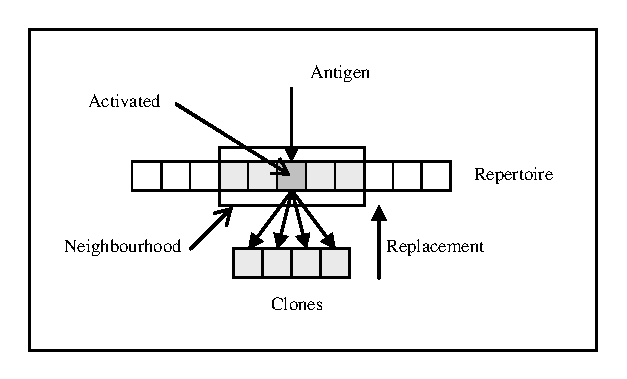
\includegraphics[scale=0.85]{Cells/cells-spatial-process}
	\caption{Depiction of clones competing in the neighbourhood of their progenitor.}
	\label{pic:cells:spatial:clones}
\end{figure}

% responsibility
The spatially restricted `back-end' selection (neighbourhood function) is expected to result in the assignment of antigenic-responsibility to regions of the spatial repertoire structure\footnote{`Back-end' refers to competition at the end of an iteration of the algorithm cycle.}. Therefore, the neighbourhood function constrain's resource allocation resulting in a localised clonal dominance effect, where those cells that win upfront selection will produce clones that dominate sub-structures in the lattice. In effect, the spatial replacement strategy facilitates a mapping of the antigenic space onto the lower-order topology of the spatial repertoire. The clonal selection axiom of `similar cells taking responsibility for similar antigen' is bonded to the lattice structure, facilitating the self-organisation of receptors to input signals. Ultimately, the expected organisation of similar cells into regions results in a broader competition between regions for activation, cloning, and the resulting ongoing retention of the region for spatial resources.
% replacement
The selection of the replacement function can play an important role in the maintenance behaviour of cell clusters. Clones are expected to have the same or similar affinity for the antigen as the activated cell given relatively low mutation rates. A clone that displaces a neighbouring cell is likely to be an activated cell in the following exposure. A similarity or affinity based replacement function is expected to maintain a cell cluster tied to a spatial locality and a random replacement function is expected to shift the centroid of the cluster around such that the fringe of the cell group may interact with neighbouring groups. In the case of the a stable spatial locality, upfront dominant cells are expected to put pressure on their neighbourhood to conform to the antigenic signals to which they dominant. Dominance leads to neighbourhood takeover which results in the emergent effect of self-organised responsibility. 

%
% Explicit and Implicit Organisation
%
\subsubsection{Explicit and Implicit Organisation}
Exploitation of the spatial structure as an upfront pressure results in the partitioning of input signals to regions of the spatial structure. This has the benefit of explicitly limiting the scope of interest of input signals space for regions of the lattice, with the problems associated with making assumptions regarding the partitioning the signal space. All resources are employed for a specific task, although not all the allocated resources may be required for their allocations. The exploitation of the spatial structure as a back-end pressure results in the implicit partitioning of the input space and self-organisation of receptor clones to take responsibility for the automatic partitions. This has the benefit of proportionate allocation (specialisation) of resources for the automatically identified complexities of the input space with the computational and delay costs for the self-organising process. Resource allocation is determined automatically, although not all resources may be utilised effectively. An interesting observation is that one method will lead to the other, such that the explicit exploitation of the spatial competition of both ends is not required. The application of upfront spatial partitioning will force regions to adapt to input signals, thus result in replacements occurring in the same region, reinforcing the partitioning. The application of back-end partitioning will self-organise the responsibility for antigenic signals via replacement, which will reinforce future input signals being directed to responsible areas of the spatial structure.

\begin{figure}[ht]
	\centering
	\begin{minipage}[c]{0.5\linewidth}
		\centering 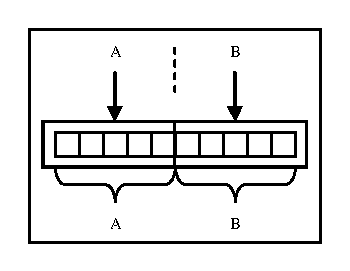
\includegraphics[scale=0.85]{Cells/cells-spatial-partition-explicit}
	\end{minipage}%
	\begin{minipage}[c]{0.5\linewidth}
		\centering 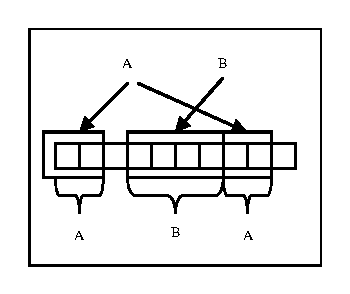
\includegraphics[scale=0.85]{Cells/cells-spatial-partition-implicit}
	\end{minipage}
	\caption{Depiction of the explicit versus implicit partitioning of input signals and the effects on the repertoire.}
	\label{pic:cells:spatial:explicit:v:implicit}
\end{figure}

%
% Empirical Study
%
\subsection{Spatial Repertoire Empirical Study}
%
% Aim
%
\subsubsection{Aim}
The aim of this investigation is to investigate cellular clonal selection constrained by a spatial repertoire structure. Toward this end, the study had the following goals:

\begin{enumerate}
	\item Investigate the effects on the repertoire composition and capability in adopting a spatial repertoire structures.
	\item Assess the effects on the repertoire in exploiting the spatial structure to localise clonal integration via replacement.
\end{enumerate}

%
% Method
%
\subsubsection{Method}

%
% Algorithms
%
\paragraph{Algorithms}
This study considers the Replacement Cellular Clonal Selection Algorithm (RCCSA), and two variations of the Spatial Cellular Clonal Selection Algorithm (SCCSA).
% RCCSA
The RCCSA defined in  Algorithm~\ref{alg:cells:realisation:algorithms:rccsa:exposure} was configured with $N_{cells}=100$, $N_{selected}=2$, and $N_{clones}=5$ to promote an allocation of ten cells per antigen in ACSP-10.
% SCCSA
Unlike RCCSA, SCCSA does not aggregate and integrate clones as a group into the repertoire, instead clones are replaced individually, with per-progenitor clonal sibling replacement exclusion. Two variations of the SCCSA algorithm were investigated: (1) a variation that organised the repertoire into a lattice although was constrained by the spatial organisation called holistic replacement (SCCSA-HR), and (2) a variation that exploited the spatial repertoire and constrained the integration of clones to the spatial neighbourhood of the progenitor cell and with exclusion of clonal siblings (like RCCSA and SCCSA-HR) called neighbourhood replacement (SCCSA-NR). The neighbourhood was defined as the square of the nine cells surrounding and including a given position in the toroidal lattice. Both SCCSA used the same configuration as RCCSA, although the lattice dimensions used the square root of $N_{cells}$ resulting in a 10-by-10 2-dimensional repertoire.

%
% Problems
%
\paragraph{Problems}
This study used the ACSP-10 problem used for the CCSA empirical study in Section~\ref{sec:cells:ccsa:ccsa}.

%
% Experiment
%
\paragraph{Experiment}
This study used the same experimental configuration including stop conditions, measures, as were used for the RCCSA empirical study in Section~\ref{sec:cells:ccsa:rcsa}, including the Average Best Matching Cells Per Antigen (ABMCPA). 
% new measures
An additional measure was used that calculated the average diversity of the 9-cell neighbourhood for each position in the lattice, called the Average Cell Neighbourhood Diversity (ACND). The diversity was calculated using the Average Cell Diversity (Equation~\ref{eq:cells:realisation:acd}) method for each neighbourhood, and averaged across all 100 neighbourhoods.

%
% Results
%
\subsubsection{Results}
% tables
Table~\ref{tab:cells:sccsa:study1} provides a summary of results for each algorithm-problem combination including the mean ($\bar{x}$) and standard deviation ($\sigma$) of collected measure values. The non-parametric Mann-Whitney~U statistical test was calculated pair-wise for all algorithms. 
% figures
Figures \ref{fig:cells:sccsa:study1:acd:boxplot}, \ref{fig:cells:sccsa:study1:ace:boxplot}, \ref{fig:cells:sccsa:study1:abmca:boxplot}, and \ref{fig:cells:sccsa:study1:acnd:boxplot} show the ACD, ACE, ABMCPA, and ACND on all algorithms respectively. 
% plots
Figure~\ref{fig:cells:sccsa:study1:plots} provides example plots of the state of the repertoire from the two spatial-based algorithms  (same configuration, random seeds of 1 and 5 for the algorithm and problem respectively). 

\begin{table}[htp]
	\centering\small
		\begin{minipage}{\textwidth}
		\begin{tabular}{llllllllll}
		\toprule
		\textbf{Problem} & \textbf{System} & \multicolumn{2}{c}{\textbf{ACD}} & \multicolumn{2}{c}{\textbf{ACE}} & \multicolumn{2}{c}{\textbf{ABMCPA}} & \multicolumn{2}{c}{\textbf{ACND}}\\
		\midrule
		\emph{ACSP} & \emph{CCSA} & $\bar{x}$ & $\sigma$ & $\bar{x}$ & $\sigma$ & $\bar{x}$ & $\sigma$ & $\bar{x}$ & $\sigma$\\
		\toprule
		ACSP-10 & RCCSA & 89.128 & 0.732 & 0.002 & 0.002 & 3.94 & 0.803 & N/A & N/A \\
		ACSP-10 & SCCSA-HR & 92.876 & 0.405 & 0.012 & 0.012 & 2.83 & 0.352 & 83.257 & 0.508 \\
		ACSP-10 & SCCSA-NR & 87.592 & 0.968 & 0.002 & 0.001 & 3.417 & 0.424 & 65.119 & 1.514 \\
		\multicolumn{2}{l}{\emph{Significant}} & True &  & True\footnote{False for RCCSA and SCCSA-NR} &  & True &  & True & \\
		\bottomrule
		\end{tabular}
		\end{minipage}
	\caption{Summary of results for SCCSA on AEP 10.}
	\label{tab:cells:sccsa:study1}
\end{table}


% graphs
\begin{figure}[htp]
	\subfloat[Average Cell Diversity (ACD) on ACSP-10.]{
	\label{fig:cells:sccsa:study1:acd:boxplot} %% label 
	\begin{minipage}[t]{0.50\textwidth}
		\centering 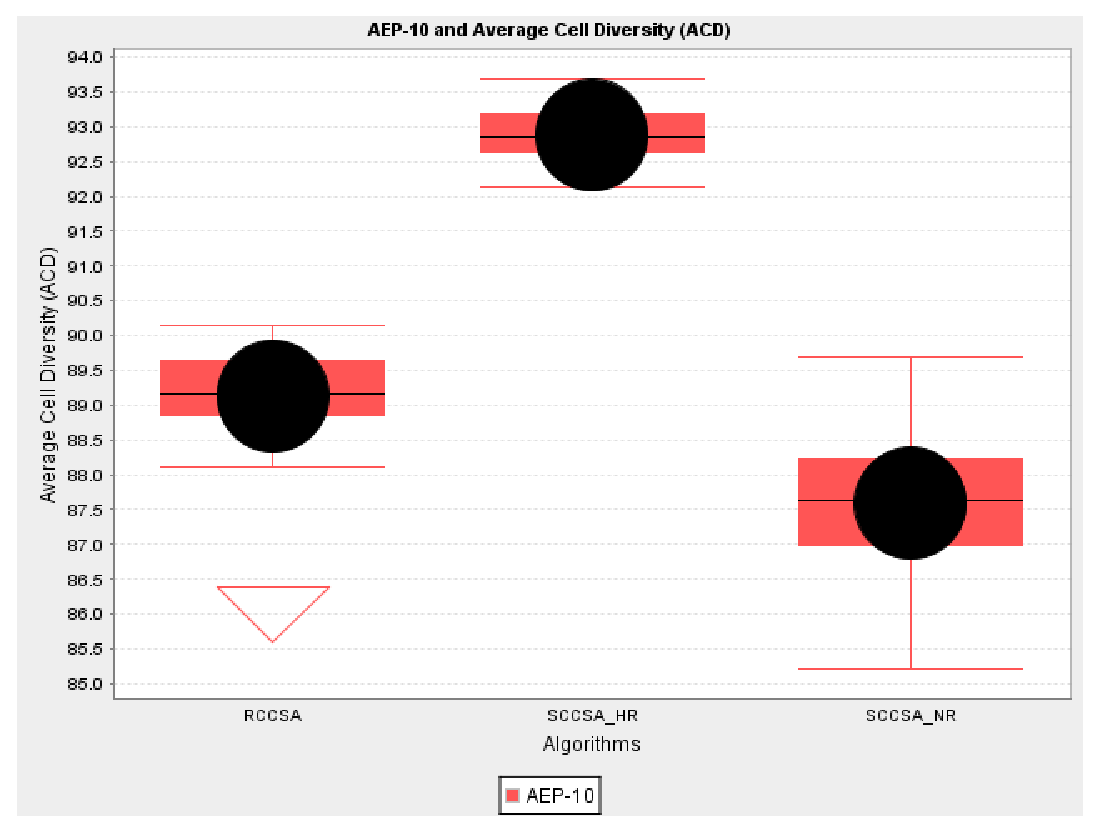
\includegraphics[scale=0.40]{Cells/SCCSA-ACD-plot}
	\end{minipage}}%
	%\hfill
	\subfloat[Average Cell Error (ACE) on ACSP-10.]{
	\label{fig:cells:sccsa:study1:ace:boxplot} %% label 
	\begin{minipage}[t]{0.50\textwidth}
		\centering 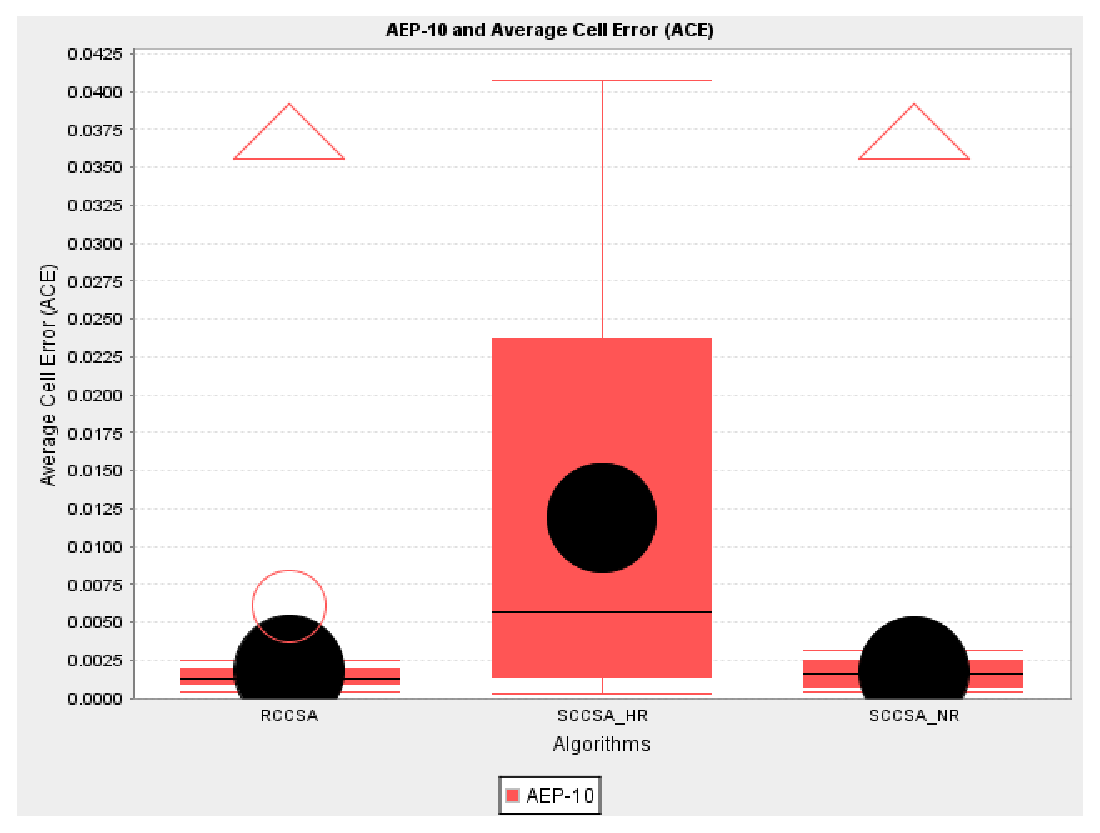
\includegraphics[scale=0.40]{Cells/SCCSA-ACE-plot}
	\end{minipage}}\\
	% new line for second set
	\subfloat[Average BMC Per Antigen on ACSP-10.]{
	\label{fig:cells:sccsa:study1:abmca:boxplot} %% label 
	\begin{minipage}[t]{0.50\textwidth}
		\centering 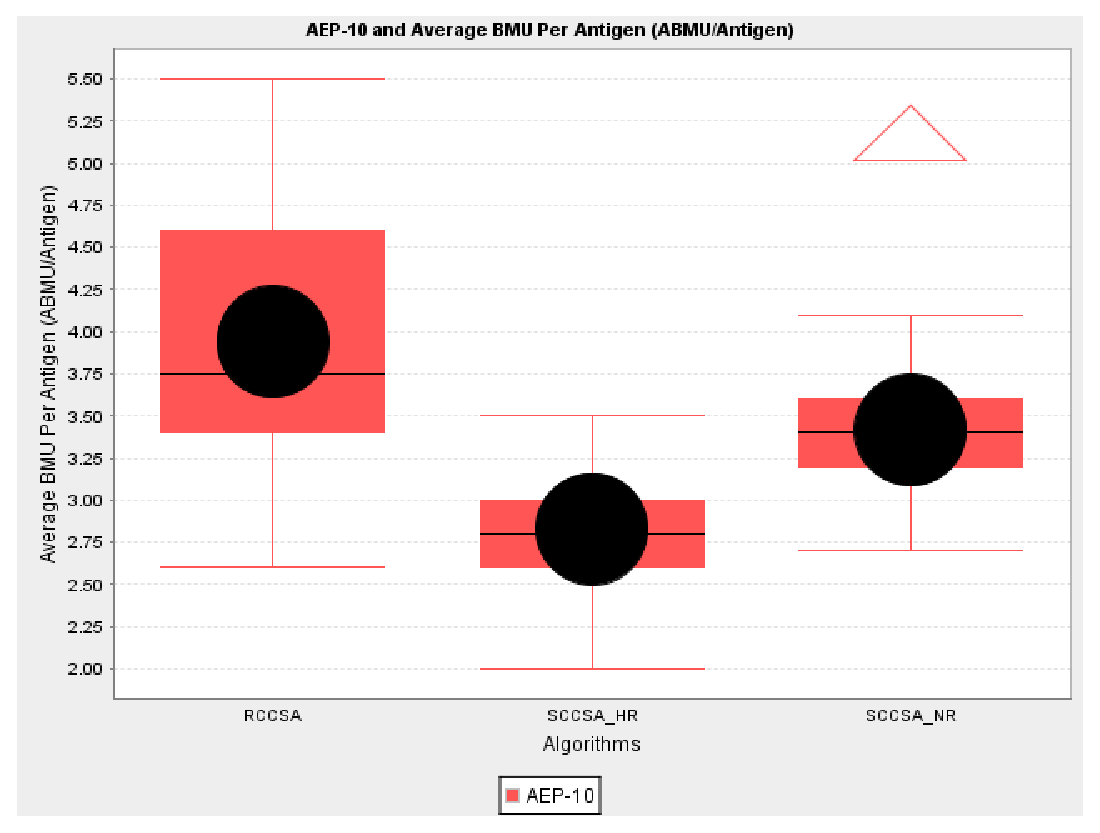
\includegraphics[scale=0.40]{Cells/SCCSA-ABMCPA-plot}
	\end{minipage}}%
	%\hfill
	\subfloat[Average Cell Neighbourhood Diversity on ACSP-10.]{
	\label{fig:cells:sccsa:study1:acnd:boxplot} %% label 
	\begin{minipage}[t]{0.50\textwidth}
		\centering 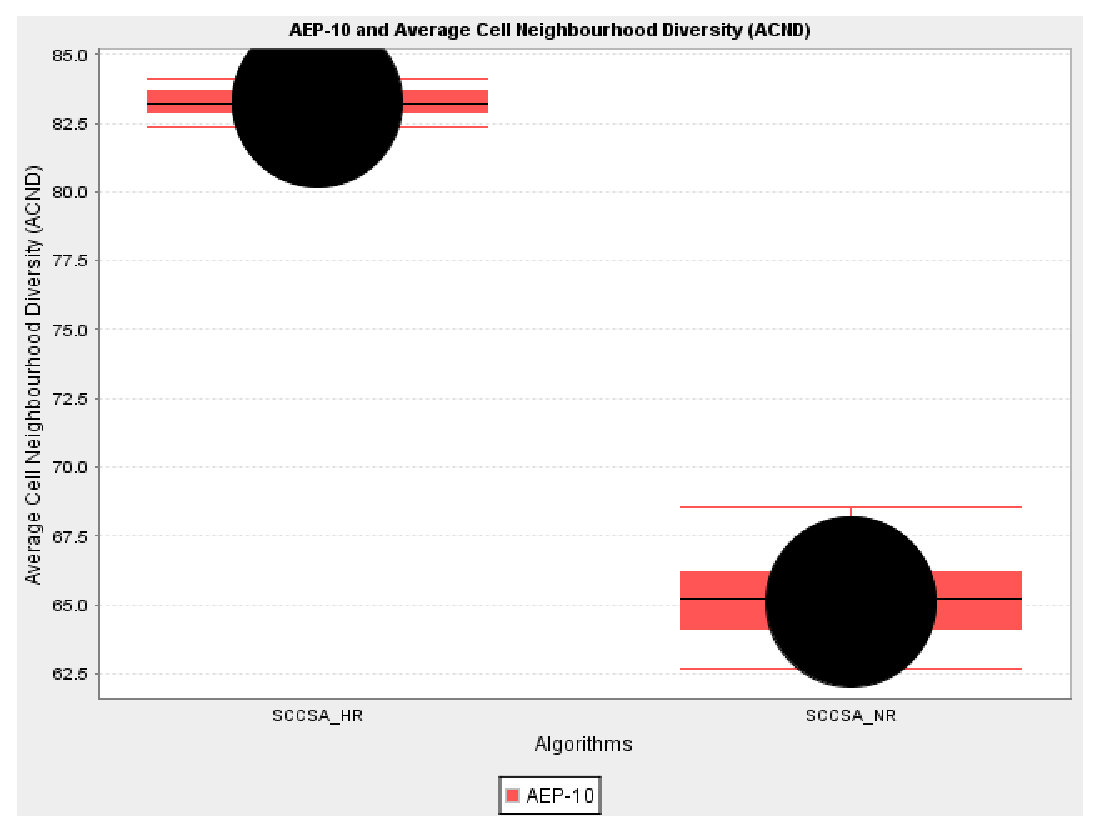
\includegraphics[scale=0.40]{Cells/SCCSA-ACND-plot}
	\end{minipage}}%
	\caption{Box-and-whisker plot's from the Spatial Repertoire Empirical Study.}
	\label{fig:tissues:sccsa:all:boxplot} %% label for entire figure
\end{figure}

% plots
\begin{figure}[htp]
	\subfloat[SCCSA-HR on ACSP-10.]{
	\label{fig:cells:sccsa:study1:a} %% label 
	\begin{minipage}[t]{0.50\textwidth}
		\centering 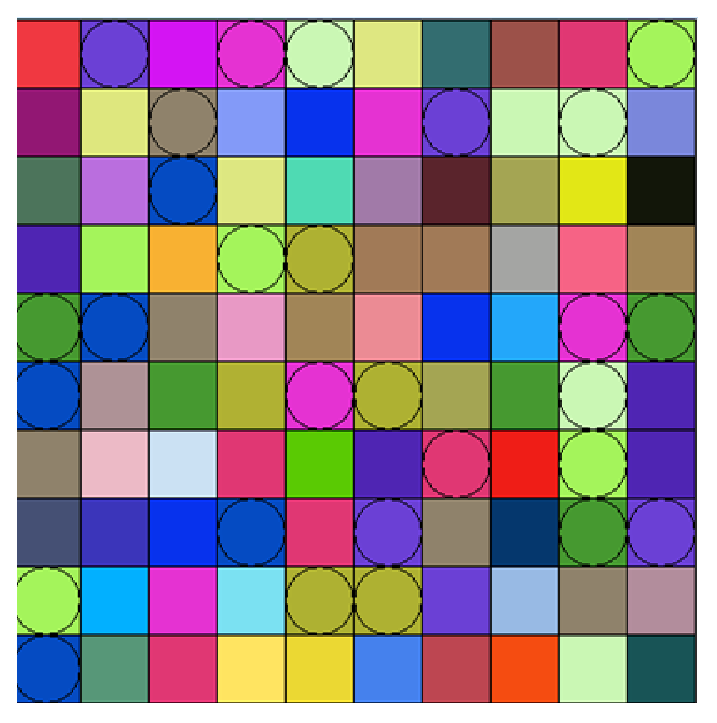
\includegraphics[scale=0.50]{Cells/SCCSA-HR-plot}
	\end{minipage}}%
	\hfill
	\subfloat[SCCSA-NR on ACSP-10.]{
	\label{fig:cells:sccsa:study1:b} %% label 
	\begin{minipage}[t]{0.50\textwidth}
		\centering 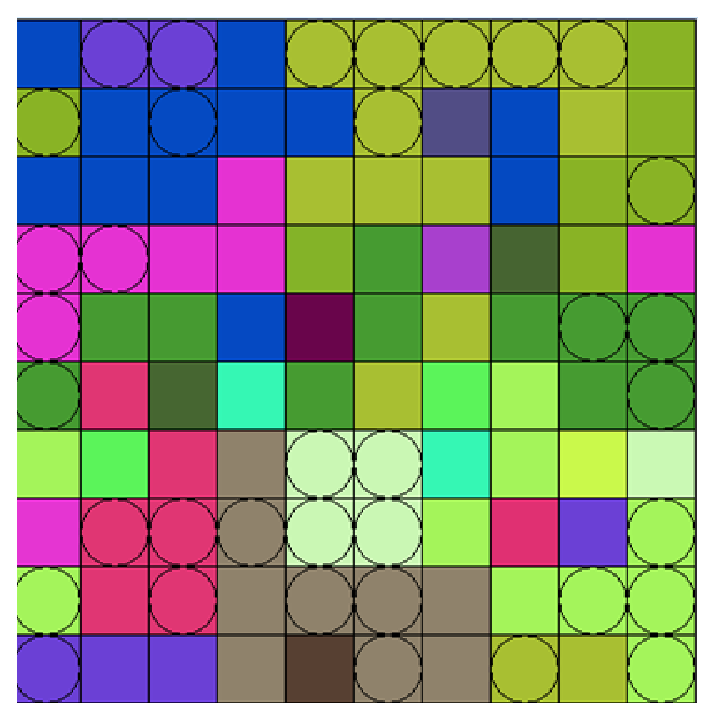
\includegraphics[scale=0.50]{Cells/SCCSA-NR-plot}
	\end{minipage}}\\
	% end
	\caption{Example plots of the spatial repertoire from two variations of SCCSA at the end of the run on ACSP-10 with BMC represented with circles.}
	\label{fig:cells:sccsa:study1:plots} %% label for entire figure
\end{figure}


%
% Analysis
%
\subsubsection{Analysis}
This section provides an analysis of the results reported in the previous section in the context of the goals of the empirical study. 

%
% Spatial Structure Trends
%
\paragraph{Spatial Structure Trends}
% section
This section considers the effects of storing the repertoire in a spatial structure by comparing the results of RCCSA to SCCSA with holistic replacement.
% measures
The use of the spatial structure in SCCSA-HR resulted in a small increase in repertoire diversity and in particular response error where ACE also showed a large increase in the variance of final ACE scores. The increase in diversity and error correlated with a decrease in the average number of BMC's.
The spatial structure was used in SCCSA-HR to hold the repertoire although was not exploited in any way. The difference in the repertoire composition and capability between the approach and RCCSA demonstrate the effect of the per-progenitor clonal set replacement used in SCCSA compared to the aggregated clonal set replacement in RCCSA.

%
% Localised Replacement Trends
%
\paragraph{Localised Replacement Trends}
% section
This section considers the exploitation of the spatial structure in the neighbourhood replacement used in SCCSA compared to holistic replacement.
% measures
The SCCSA-NR resulted in a the increased organisation of the repertoire as expected by localising cells for the same antigen into areas on the spatial repertoire structures. This was demonstrated by the decrease in repertoire diversity compared to both SCCSA-HR and RCCSA, and a small increase in ABMCPA compared to SCCSA-NR. Interesting the exploitation of spatial neighbourhood competition resulted in a ACE not significantly different from RCCSA, suggesting that such competition results in the same level of per-antigen specialisation within the repertoire as RCCSA. Importantly the increased organisation was demonstrated by the significant decrease in average repertoire diversity compared to holistic replacement, which was depicted in the example plot in Figure~\ref{fig:cells:sccsa:study1:plots} showing that this decrease was caused as a result of the clear grouping of similar cells (similar colours) in the spatial repertoire.

%
% Conclusions
%
\subsubsection{Conclusions}
This section summarises the findings of the empirical study into the Spatial Cellular Clonal Selection Algorithm in terms of the primitives that were the focus of the study and the expectations that motivated the study.

\begin{enumerate}
	\item Neighbourhood replacement provides intra-clone competition that results in similar general behaviours as consolidating the clone for replacement in RCCSA.
	\item Neighbourhood replacement results in the spatial localisation of clones on the lattice, the so called spatial responsibility effect as expected.
\end{enumerate}

%
% Response Mediation
%
\section{Response Mediation}
\label{sec:cells:mediated}
This section elaborates on the clonal selection by introducing a second repertoire of intermediate (mediator) cells to provide an adaptive context for localising the differential resource allocation of clonal selection, providing a model of decoupled \emph{feature detection} and \emph{system response}. 

%
% Mediated Clonal Selection
%
\subsection{Mediated Clonal Selection}
% metaphor
Two-signal theories have been proposed in immunology as verification signals permitting the proliferation and differentiation of lymphocytes. Historically developed for the activation of B-lymphocytes (in the context of self-nonself discrimination), the two-signal approach has also been extended to the various classes of T-cells. The dominant type of B-cell activation is dependant on Helper T-cells that identify MHC molecules on the surface of activated antigen-presenting B-cells. The detection of MHC provides a secondary verification signal to the B-cells, allowing them to proliferate and differentiate. This process is called the co-stimulation of B-cells by T-cells or T-cell dependant activation of B-cells. Likewise, T-cell activation requires an antigen specific signal via an antigen-presenting cell and a co-stimulating `antigen non-specific' verification signal. The theory of the two-signal activation of T-cells is called associative recognition theory \cite{Bretscher1970}.

% abstraction
\emph{Mediated Clonal Selection} or so-called inter-repertoire recognition decomposes the clonal selection process such that a mediation process is responsible for selecting those cells from the activated set that may proliferate. The mediation process is controlled by a sister repertoire of cells that also perform a clonal selection process using the activated cells of the first repertoire as input signals. The Helper T-cell metaphor is adopted such that the repertoire of cells (first repertoire) represents B-lymphocytes, which require a second verification signal from the helper T-lymphocytes (second repertoire) before proliferating and differentiating. After providing the secondary signal to the activated set of B-lymphocytes, the helper T-lymphocytes proceed with the cloning and maturation of the activated T-cells. Therefore, the T-cell repertoire is an application of the clonal selection algorithm that accepts the activated set of another clonal selection algorithm as a pseudo-`antigenic set'. Two concerns that must be reconciled in integrating the two repertoires are as follows: (1) The T-cells must select those B-cells from the B-cells activated set that may proliferate (2) The B-cell activated set provides multiple antigens simultaneously to the T-cell repertoire, to which it is possible to generate a T-cell activated set for each member of the B-cell activated set. The remainder of this section considers the implications of the second clonal selection governed repertoire from a variety of different perspectives.

% 
% Mapping Function
%
\subsubsection{Mapping Function}
% verification signal
The proliferation \emph{verification signal} for the activated B-cell's may be \emph{antigen-dependent} or \emph{antigen-independent}. If antigen-dependent, the information provided by the verification signal may be considered a generalisation of the input signals provided to the B-cell repertoire. If the verification signal is antigen-independent, then the information provided is a generalisation of the cells themselves in the B-cell repertoire. This is a subtle but potentially important difference that effects the representation of information by the system.

% about dependant
An antigen-dependent mapping from B-cell to T-cell requires that some regularities of the input signal are preserved. The transformation may be of the whole antigen itself, or just the part of the antigen recognised by the B-cell receptor. The T-cell repertoire adapts to a consistent (B-cell invariant) generalisation of the antigenic input patterns. An antigen-dependent mapping between the repertoires provides a top-down organisation of the relationship between the repertoires, where simply matching onto the second repertoire provides the verification signal.
% about independent
A potential concern with antigen dependence is that the mapping of the input patterns may be achieved in one repertoire, making the second repertoire redundant. An antigen-independent mapping disregards the regularities of the input signal, such that the T-cell is performing pattern recognition of B-cell receptors, rather than a pattern recognition of antigen (whether symbolic or sub-symbolic). The result is a T-cell repertoire that is developed independent of antigen, and dependent on the B-cell repertoire (which in turn develops in response to antigen). A potential concern with an antigen-independent mapping is that it is arbitrary such that T-cells are completely dependent on specific B-cell lineages, and regularity between B-cell patterns has no meaning other than ancestry (likely to make the mapping harder). 

%
% Formation of High-Order Structures
%
\subsubsection{Formation of High-Order Structures}
% general
Interestingly, the relationship between an antigen and cells, as well as cells between repertoires may be considered in the context of the formation and maintenance of higher-order structures.
% consider a single repertoire
For example in the case of a single repertoire, one antigen may map onto one cell providing a specialised mapping. This may be elaborated to include the extremes cardinality of relationship. For example, a one-to-many relationship between antigen and cells maybe considered a decomposition of feature extraction, particularly if the mapping is partial or sub-symbolic. Additionally, many antigen may be mapped onto many cells either directly (generalisation of one-to-one) or partially (cross reactivity), or onto a single cell, compressing the signal.

% consider relationships between repertoires
The relationship between repertoires adds a second level of complexity to the hierarchical structure. The same relationships apply although in this case between cells, with the importance difference that the relationships can be manipulated with mapping schemes, activated B-cell set size, and activated T-cell set size.
% control
For example, it may be desirable to coerce the B-cell repertoire to decompose antigen into regular features (many), and the T-cell receptor to generalise those features toward a specific meaning (few). Alternatively, the B-cell repertoire may be coerced to generalise (compress) based on common antigenic features (few), and the T-cell repertoire to decompose the B-cell information content into a variety of different meanings (many).

\begin{figure}[htp]
	\subfloat[Many-to-One.]{	
	\begin{minipage}[t]{0.50\textwidth}
		\centering 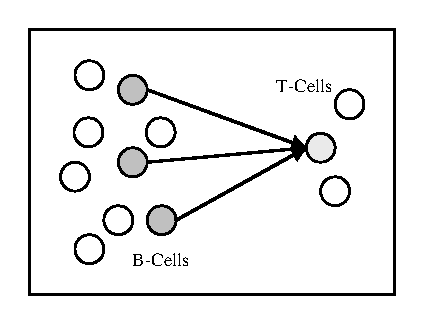
\includegraphics[scale=0.70]{Cells/mediated-many-to-one}
	\end{minipage}}%
	\hfill
	\subfloat[One-to-Many.]{	
	\begin{minipage}[t]{0.50\textwidth}
		\centering 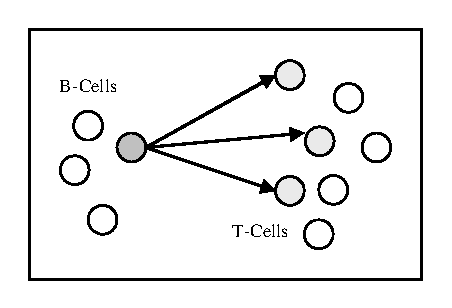
\includegraphics[scale=0.70]{Cells/mediated-one-to-many}
	\end{minipage}}\\
	% end
	\caption{Depiction of inter-repertoire structures based on the mapping of cells.}
	\label{fig:cells:mediated:structures} %% label for entire figure
\end{figure}

% altered activation scheme
Rather than treating each activated B-cell independently, the activated B-cells may interact with the T-cell population concurrently, such that multiple B-cells may activate a single T-cell. The T-cell repertoire may be configured such that a T-cell is required to match more than one B-cell before it may become activated. This provides a mechanism in which the T-cell repertoire facilitates the aggregation of multiple antigenic features into a single T-cell. The second repertoire facilitates the addition of a second layer of meaning. In the many-to-one case a T-cell may represent a high-order concept as an aggregate of multiple lower-level concepts (B-cells). The meaning is a single or small collection of concepts that are dependent on the presence of specific features (specific context). 
% examples
For example, \emph{Many-to-One} provides a consensus forming operation in which many lower-order concepts (such as extracted features) are aggregated together to form a high-order concept. The \emph{One-to-Many} relationship provides a descriptive operation in which a high-order concept is decomposed into a number of lower-order concepts (such as descriptive features). In both of these examples, the meaning implies a mapping that manages to preserve some regularities of the input signal, such that higher-order or lower-order concepts may be described. 

%
% Supervised Concept Formation
% 
\subsubsection{Supervised Concept Formation}
The incorporation of additional feedback into the algorithm allows an external process to assign meaning and supervise the mapping and formation of concepts. For the single repertoire algorithm, T-cell mediation provides an immunologically plausible basis for feedback (verification) to supervise the selection of activated receptor patterns in response to antigenic exposures. For the dual repertoire algorithm, tissue damage provides an immunologically plausible basis for feedback to supervise the selection of concepts formed in the T-cell repertoire, which in turn feeds back to the B-cell repertoire via the mediation process. The proposed integration of feedback results in two flows of information through the system. The top-down flow of antigenic signals results in B-cell receptors competing for activation, and T-cell receptors competing for activation of the B-cell receptor activated set. Those B-cells that receive the secondary signal, proliferate. The bottom-up flow of tissue-damage input results in T-cells competing for encouragement that the concepts that they represent are \emph{useful}. Those T-cells that receive a positive (non-negative, and perhaps non-neutral) feedback, proliferate. Therefore, the application of feedback (if available) is to the activated set of T-cells. In the absence of feedback, there is simply the absence of corrective behaviour: the punishment, or reward of the activated T-cell concept.


\begin{figure}[htp]
	\subfloat[Many-to-Few.]{	
	\begin{minipage}[t]{0.50\textwidth}
		\centering 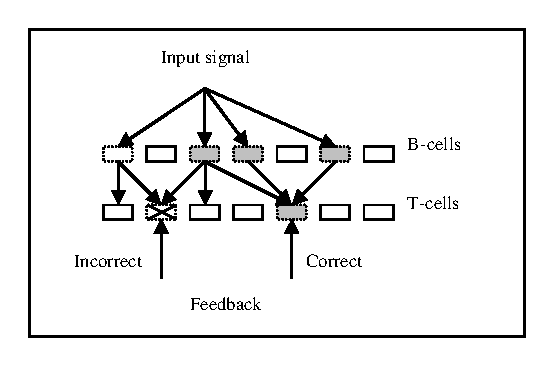
\includegraphics[scale=0.85]{Cells/mediated-many-to-few}
	\end{minipage}}%
	\hfill
	\subfloat[Few-to-Many.]{	
	\begin{minipage}[t]{0.50\textwidth}
		\centering 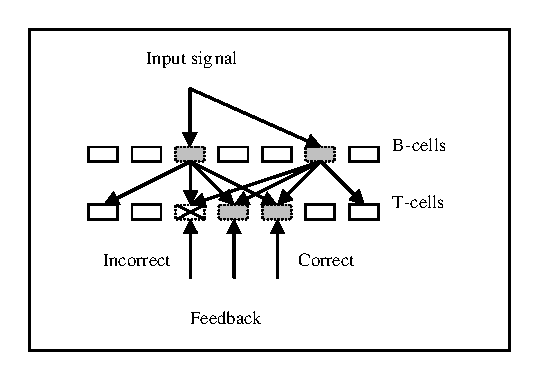
\includegraphics[scale=0.82]{Cells/mediated-few-to-many}
	\end{minipage}}\\
	% end
	\caption{Depiction of the integration of feedback for supervised structure formation.}
	\label{fig:cells:mediated:supervised} %% label for entire figure
\end{figure}

% on supervision
Bottom-up supervision of concept formation provides a natural agenda for investigating mediated clonal selection beyond the basic principles of mappings and structure formation and maintenance (for example, see Figure~\ref{fig:cells:mediated:supervised}). The integration of a feedback mechanism provide a natural relationship with the study of Reinforcement Learning (Section~\ref{subsec:cs:related:rl}).

%
% Mediated Empirical Study
%
\subsection{Mediated Empirical Study}
%
% Aim
%
\subsubsection{Aim}
The aim of this investigation was to asses the cellular clonal selection algorithm constrained by inter-cellular repertoire interactions. Toward this end, the study had the following goals:

\begin{enumerate}	
	\item Assess the behaviour of different inter-repertoire antigen-dependant mapping schemes.
	\item Investigate the effects of varied cellular cardinality in the relationships exploited via inter-repertoire mapping.
\end{enumerate}

%
% Method
%
\subsubsection{Method}

%
% Problems
%
\paragraph{Problems}
This study used the ACSP-10 problem used for the CCSA empirical study in Section~\ref{sec:cells:ccsa:ccsa}.

%
% Algorithms
%
\paragraph{Algorithms}
Algorithm~\ref{alg:cells:mediated:mccsa:exposure} defines the Mediated Cellular Clonal Selection Algorithm (ECCSA), where $Exposure(A, T)$ is a modified version of the $Exposure$ operation for RCCAS (defined in Algorithm~\ref{alg:cells:realisation:algorithms:rccsa:exposure}) that returns the selected set rather than the best matching cell. The RCCSA uses clonal sibling exclusion and a Hamming similarity function during replacement.

\begin{algorithm}[htp]
  \SetLine
  \SetKwData{Antigen}{A}
  \SetKwFunction{Exposure}{Exposure}
  \SetKwFunction{SelectBestMatchingCell}{SelectBestMatchingCell}
  
  \KwIn{\Antigen, $T_{bcells}$, $T_{tcells}$, $N_{bc-selection}$, $N_{bc-clones}$, $N_{tc-selection}$, $N_{tc-clones}$, $P_{mutation}$}
	\KwOut{$T_{rs}$}	
	
	$T_{rs} \leftarrow$0\;
	% expose the b cells
	$T_{bc-rs}$ = \Exposure{\Antigen, $T_{bcells}$, $N_{bc-selection}$, $N_{bc-clones}$, $P_{mutation}$}\;
	% expose the t cells
	$T_{tc-rs}$ = \Exposure{$T_{bc-rs}$, $T_{tcells}$, $N_{tc-selection}$, $N_{tc-clones}$, $P_{mutation}$}\;	
	% return it
	$T_{rs} \leftarrow$ \SelectBestMatchingCell{$T_{tc-rs}$}\;
	\Return{$T_{rs}$}\;
	\caption{Exposure Function for Mediated Cellular Clonal Selection.}
	\label{alg:cells:mediated:mccsa:exposure}
\end{algorithm}	

% mapping
The modified RCCSA \emph{Exposure} operation also permits the mapping of a selected set of cells ($T_{rs}$) to be treated as an antigen. This is achieved through use of an exposure operation that provides a mapping function that aggregates affinity for a given cell against a stimulating set of cells. The first part of this study considers two different examples of the mapping function: (1) Euclidean Mapping, and (2) Hamming Mapping. The affinity scores are aggregated within each cell of the repertoire against the stimulating set to provide a general indication of a cells capability against a stimulating set. In this part of the study, both the B-cell and T-cell repertoires used identical configurations as follows: $N_{cells}=100$,  $N_{selected}=1$, $N_{clones}=10$ (10\% of each repertoire per antigen).
% relationship
The second part of the study considered varied relationships between the two repertoires in terms of the size of the selected B-cell set which stimulates the T-cell repertoire, and the size of of the activated and responding T-cell set. A series of one-to-one and many-to-many relationships were assessed with the intermediates, where the number of clones and this repertoire assigned per antigen was kept constant at six (10\% of each repertoire per antigen) with regard to the selection size. The configurations are summarised in Table~\ref{tab:cells:mccsa:mappings:configuration}. A Euclidean mapping was used between the repertoires in this second part of the study.

\begin{table}[htp]
	\centering\small
		\begin{tabular}{lllllll}
		\toprule
		\textbf{Relationship} & \multicolumn{3}{c}{\textbf{B-Cells}} & \multicolumn{3}{c}{\textbf{T-Cells}} \\ 
		\midrule
		\emph{Name} & $N_{b-cells}$ & $N_{bc-selected}$ & $N_{bc-clones}$ & $N_{t-cells}$ & $N_{tc-selected}$ & $N_{tc-clones}$ \\ 
		\toprule
		\emph{1-to-1} & 60 & 1 & 6 & 60 & 1 & 6 \\ 
		\emph{1-to-N} & 60 & 1 & 6 & 60 & 6 & 1 \\ 
		\emph{N-to-1} & 60 & 6 & 1 & 60 & 1 & 6 \\ 
		\emph{N-to-N} & 60 & 6 & 1 & 60 & 6 & 1 \\ 
		\bottomrule
		\end{tabular}
	\caption{Summary of the configuration of the ECCSA with a series of inter-repertoire selection relationships.}
	\label{tab:cells:mccsa:mappings:configuration}
\end{table}

%
% Experiment
%
\paragraph{Experiment}
This study used the same general experimental configuration including stop conditions as were used for the CCSA empirical study in Section~\ref{sec:cells:ccsa:ccsa}. 
% new measures
A series of new measures were defined for the experiment. The Average Cell Diversity measure (defined in Equation~\ref{eq:cells:realisation:acd}) was calculated for each of the B-cell and T-cell repertoires referred to as the Average B-Cell Diversity (ABCD), and the Average T-Cell Diversity (ATCD) respectively. This treatment was performed to the Average Cell Error measure (defined in Equation~\ref{eq:cells:realisation:measure:ace}) referred to as the Average B-Cell Error (ABCE) and the Average T-Cell Error (ATCE) respectively, where the measure was taken as the best response from each repertoire against the antigen. The Average BMC per Antigen (defined in Equation~\ref{eq:cells:ccsa:rcca:abmcpa}) was adapted for the two re-repertoire configuration referred to as the Average Best Matching B-Cells Per Antigen (ABMBCPA) and the Average Best Matching T-Cells Per Antigen (ABMTCPA) respectively.
% system response
The system's response was taken as the best matching cell from the set of selected (activated) T-cells for each antigen exposure, called the Response Error (RE).
% mapping measure
A new measure was defined that calculated the T-cell error after mapping, averaged across each cell in the T-cell repertoire called the Average T-Cell Mapping Error (ATCME). This measure provided a general indication of the mapping error between the repertoire in the units of the specific mapping scheme used. The measure was also taken against just the set of T-cells activated and selected by the activated B-cells called the Average T-Cell Selected Set Mapping Error (ATCSSME).
% figure
Figure~\ref{fig:mccsa:measures} provides a depiction of the repertoires, the antigen, the selected sub-sets and the system response as well as how all the collected measures relate to these principle attributes of the ECCSA.

\begin{figure}[htp]
	\centering
		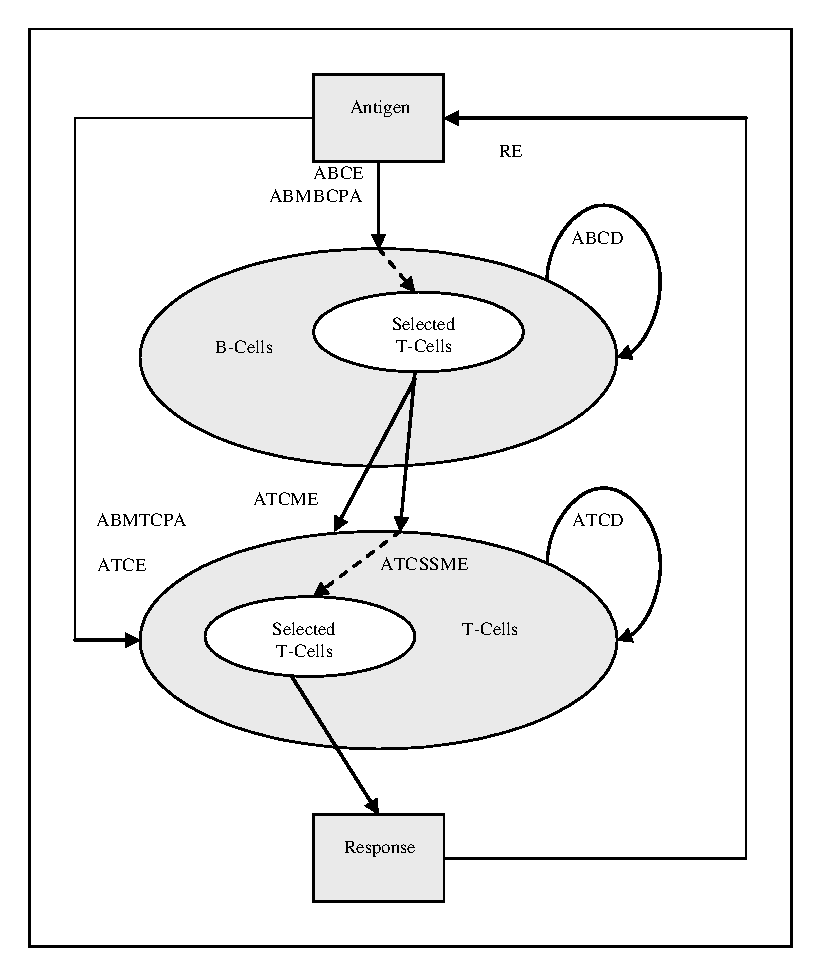
\includegraphics[scale=0.75]{Cells/MCCSA-measures}
	\caption{Depiction of the principle concerns of the MCCSA and the relationships in terms of the selected measures.}
	\label{fig:mccsa:measures}	
\end{figure}


%
% Results
%
\subsubsection{Results}
% tables
Table~\ref{tab:cells:mccsa:mappings} and Table~\ref{tab:cells:mccsa:relationships} provide a summary of results for each algorithm-problem combination including the mean ($\bar{x}$) and standard deviation ($\sigma$) of collected measure values. The non-parametric Mann-Whitney~U statistical test was calculated pair-wise for all algorithms. 
% mappings
%Figure~\ref{fig:cells:mccsa:study1:re:boxplot} shows RE, and Figure~\ref{fig:cells:mccsa:study1:plots} provide example plots for the mapping part of the study. 
% relationships 
Figures \ref{fig:cells:mccsa:study2:abcd:boxplot}, \ref{fig:cells:mccsa:study2:abce:boxplot}, \ref{fig:cells:mccsa:study2:atcd:boxplot}, \ref{fig:cells:mccsa:study2:atce:boxplot}, and \ref{fig:cells:mccsa:study2:re:boxplot} show the ABCD, ABCE, ATCD, ATCE, and RE respectively. Figure~\ref{fig:cells:mccsa:relationships:plots} provide example plots for all four configurations on the second relationship part of the study. 
% plots
Results from all example plots are taken from the end of the run with algorithm and problem configurations matching those used during experimentation, and a random number generator seed of 1 and 5 for the algorithm and problem respectively.

% comparison in the mappings
\begin{table}[htp]
	\centering\small
		\begin{tabular}{lllllc}
		\toprule
		\textbf{Measure} & \multicolumn{2}{c}{\textbf{Euclidean}} & \multicolumn{2}{c}{\textbf{Hamming}} & \textbf{Significant} \\ 
		\midrule
		 & $\bar{x}$ & $\sigma$ & $\bar{x}$ & $\sigma$ &  \\ 
		\toprule
		\emph{ABCD} & 89.399 & 0.822 & 89.399 & 0.822 & False \\ 
		\emph{ATCD} & 89.234 & 0.718 & 87.999 & 0.94 & True \\ 
		\emph{ABCE} & 0.003 & 0.002 & 0.003 & 0.002 & False \\ 
		\emph{ATCE} & 0.009 & 0.006 & 0.098 & 0.029 & True \\ 
		\emph{RE} & 0.009 & 0.006 & 0.617 & 0.123 & True \\ 
		\bottomrule
		\end{tabular}
	\caption{Summary of results for ECCSA with two different mapping schemes on ACSP-10.}
	\label{tab:cells:mccsa:mappings}
\end{table}

% figures of the mappings
%\begin{figure}[htp]
%	\centering
%		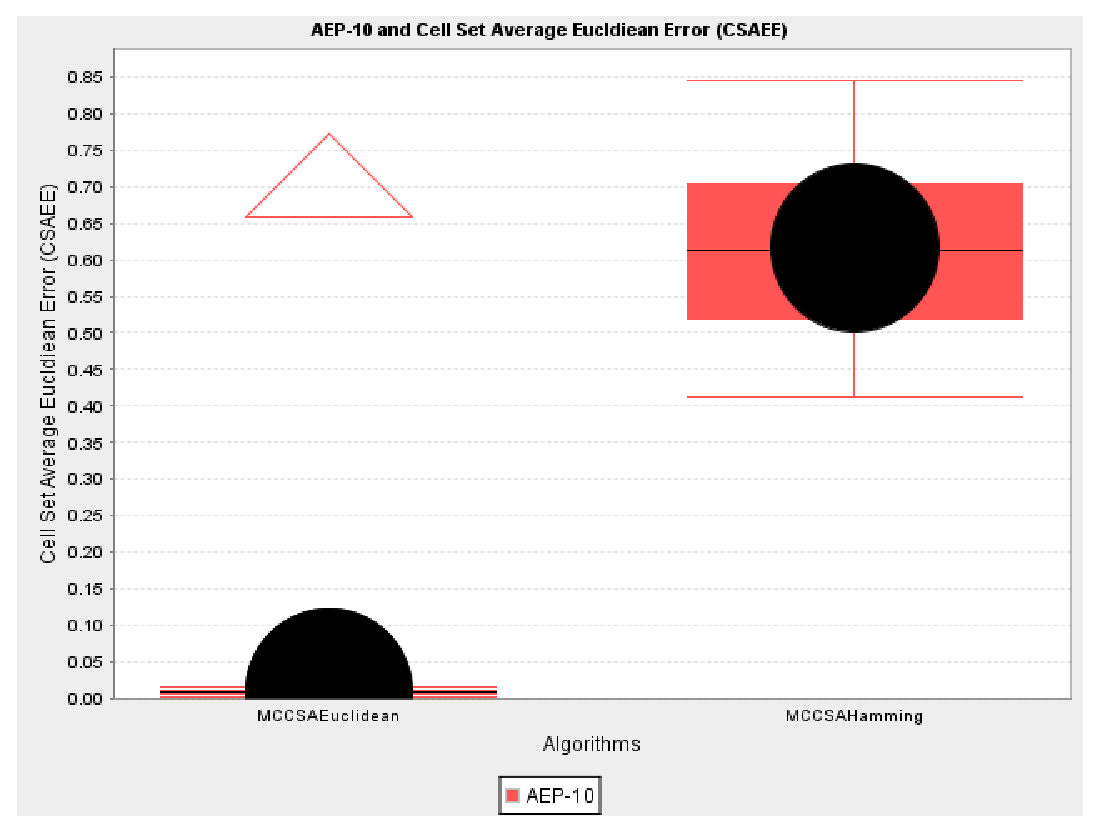
\includegraphics[scale=0.35]{Cells/MCCSA-Study1-MR}
%	\caption{Box-and-whisker plot of the Response Error of the two different mapping schemes on ACSP-10.}
%	\label{fig:cells:mccsa:study1:re:boxplot}
%\end{figure}

% plots of the mappings
\begin{figure}[htp]
	\subfloat[MCCSA-Euclidean on ACSP-10.]{
	\label{fig:cells:mccsa:study1:a} %% label 
	\begin{minipage}[t]{0.50\textwidth}
		\centering 
\includegraphics[scale=0.45]{Cells/MCCSAEuclidean-plot}
	\end{minipage}}%
	\hfill
	\subfloat[MCCSA-Hamming on ACSP-10.]{
	\label{fig:cells:mccsa:study1:b} %% label 
	\begin{minipage}[t]{0.50\textwidth}
		\centering 
\includegraphics[scale=0.45]{Cells/MCCSAHamming-plot}
	\end{minipage}}\\
	% end
	\caption{Example plots of the B- (top of each plot) and T-Cell (bottom of each plot) repertoires from the ECCSA at the end of the run on ACSP-10 for two different inter-repertoire mapping types.}
	\label{fig:cells:mccsa:study1:plots} %% label for entire figure
\end{figure}


% relationships
\begin{table}
	\centering\small
		\begin{minipage}{\textwidth}
		\begin{tabular}{llllllllll}
		\toprule
		\textbf{Measure} & \multicolumn{2}{c}{\textbf{(1-1)}} & \multicolumn{2}{c}{\textbf{(1-N)}} & \multicolumn{2}{c}{\textbf{(N-1)}} & \multicolumn{2}{c}{\textbf{(N-N)}} & \textbf{Sig.} \\ 
		\midrule
		 & $\bar{x}$ & $\sigma$ & $\bar{x}$ & $\sigma$ & $\bar{x}$ & $\sigma$ & $\bar{x}$ & $\sigma$ &  \\ 
		\toprule
		\emph{ABCD} & 88.333 & 0.812 & 87.967 & 0.721 & 94.419 & 0.113 & 94.408 & 0.147 & True \\ 
		\emph{ATCD} & 88.005 & 0.755 & 94.298 & 0.146 & 88.103 & 0.924 & 94.309 & 0.105 & True \\ 
		\emph{ABCE} & 0.027 & 0.024 & 0.028 & 0.012 & 0.067 & 0.014 & 0.067 & 0.015 & True \\ 
		\emph{ATCE} & 0.052 & 0.021 & 0.076 & 0.015 & 0.102 & 0.019 & 0.093 & 0.013 & True \\ 
		\emph{ATCME} & 0.604 & 0.065 & 0.648 & 0.04 & 3.523 & 0.307 & 3.845 & 0.188 & True \\ 
		\emph{ATCSSME} & 0.042 & 0.02 & 0.158 & 0.023 & 0.844 & 0.129 & 1.161 & 0.121 & True \\ 
		\emph{ABMBCPA} & 2.713 & 0.33 & 3.13 & 0.426 & 1 & 0 & 1 & 0 & True\footnote{False for ECCSA(N-1) and ECCSA(N-N)} \\ 
		\emph{ABMTCPA} & 3.25 & 0.318 & 1 & 0 & 2.597 & 0.549 & 1 & 0 & True\footnote{False for ECCSA(1-N) and ECCSA(N-N)} \\ 
		\emph{RE} & 0.059 & 0.031 & 0.083 & 0.016 & 0.112 & 0.022 & 0.122 & 0.019 & True\footnote{False for ECCSA(N-1) and ECCSA(N-N)} \\ 
		\bottomrule
		\end{tabular}
		\end{minipage}
	\caption{Summary of results for ECCSA with four different inter-repertoire relationship schemes on ACSP-10.}
	\label{tab:cells:mccsa:relationships}
\end{table}

% figures of the relationships
\begin{figure}[htp]
	\subfloat[Average B-Cell Diversity (ABCD) on ACSP-10.]{
	\label{fig:cells:mccsa:study2:abcd:boxplot} %% label 
	\begin{minipage}[t]{0.50\textwidth}
		\centering 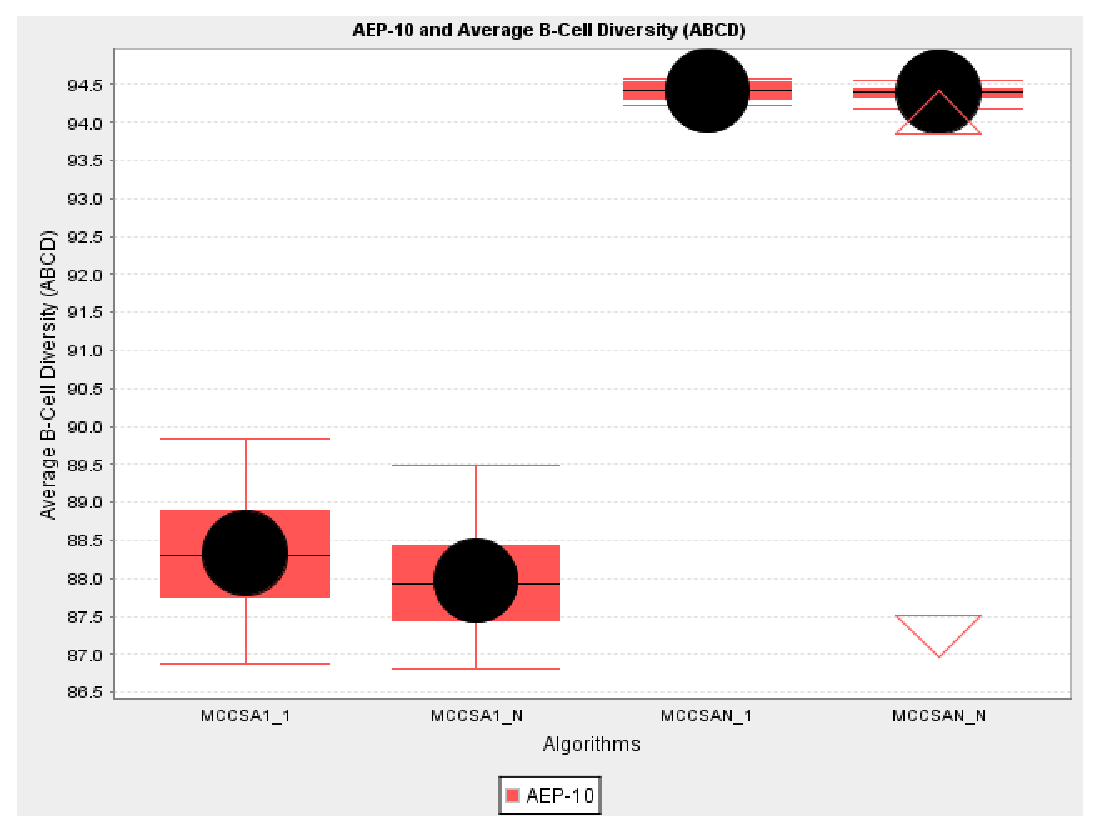
\includegraphics[scale=0.40]{Cells/MCCSA-relationships-ABCD}
	\end{minipage}}%
	%\hfill
	\subfloat[Average B-Cell Error (ABCE) on ACSP-10.]{
	\label{fig:cells:mccsa:study2:abce:boxplot} %% label 
	\begin{minipage}[t]{0.50\textwidth}
		\centering 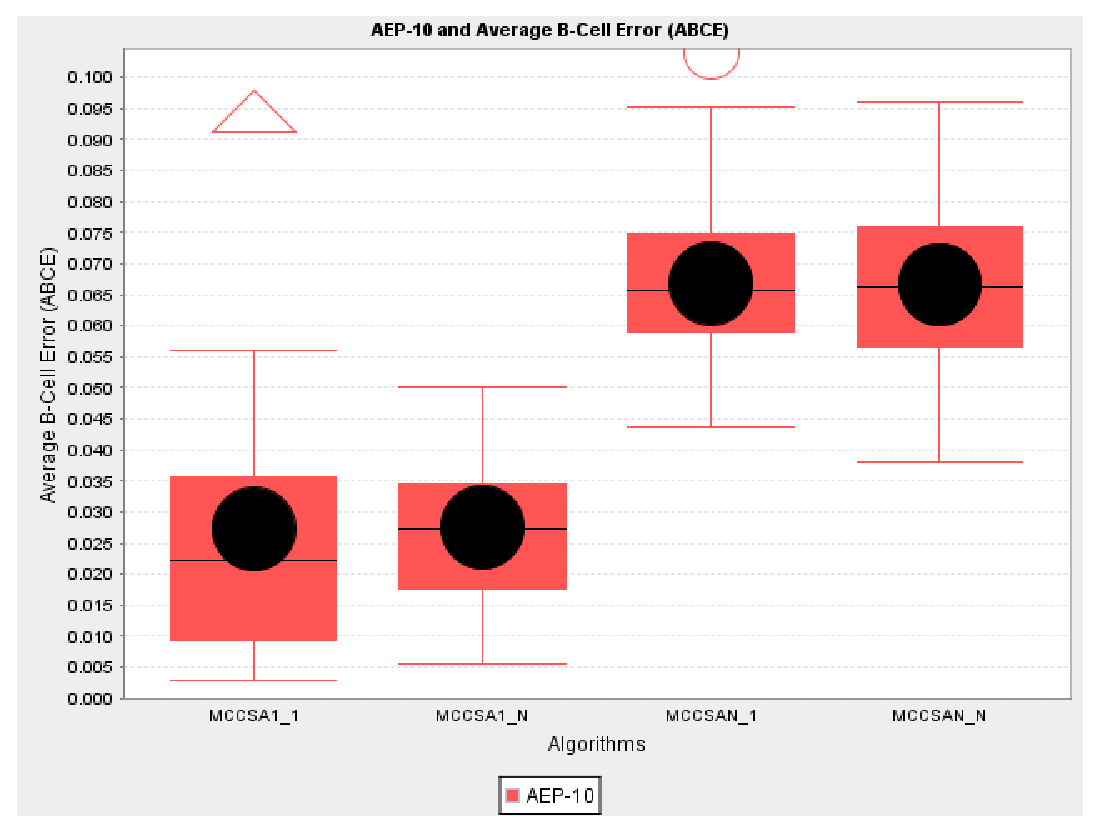
\includegraphics[scale=0.40]{Cells/MCCSA-relationships-ABCE}
	\end{minipage}}\\
	% new line for second set
	\subfloat[Average T-Cell Diversity (ATCD) on ACSP-10.]{
	\label{fig:cells:mccsa:study2:atcd:boxplot} %% label 
	\begin{minipage}[t]{0.50\textwidth}
		\centering 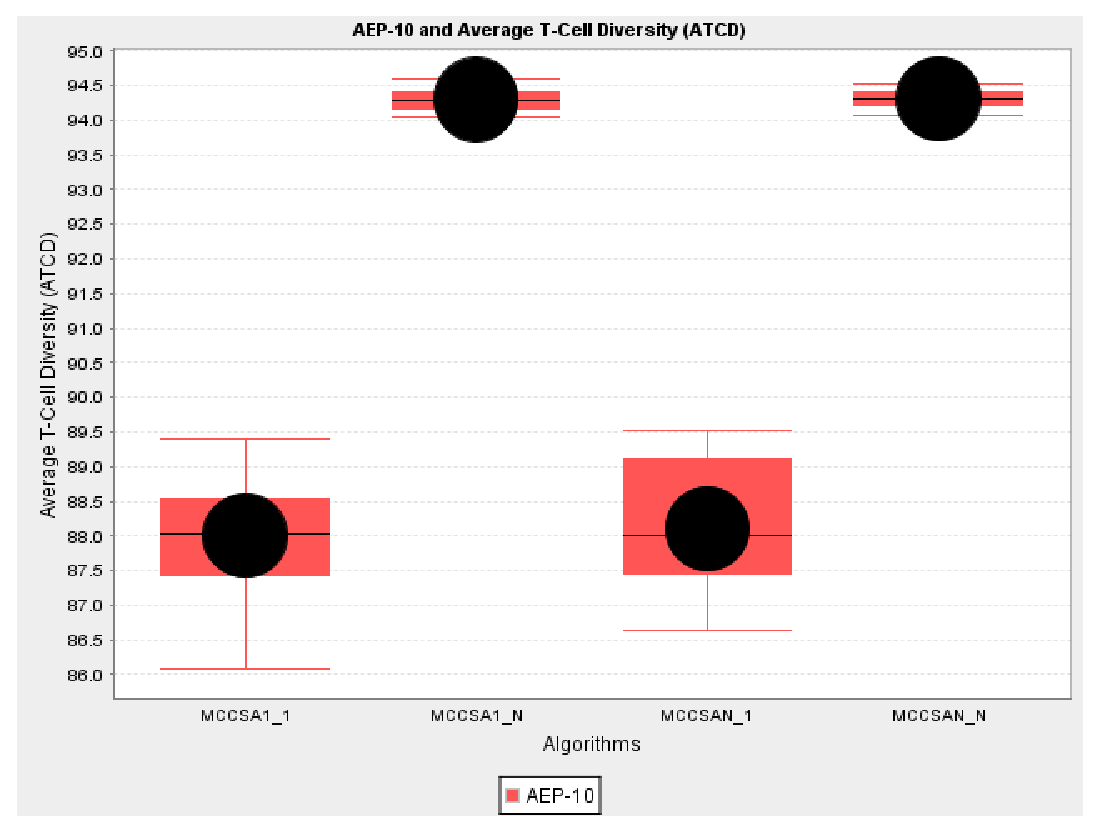
\includegraphics[scale=0.40]{Cells/MCCSA-relationships-ATCD}
	\end{minipage}}%
	%\hfill
	\subfloat[Average T-Cell Error (ATCE) on ACSP-10.]{
	\label{fig:cells:mccsa:study2:atce:boxplot} %% label 
	\begin{minipage}[t]{0.50\textwidth}
		\centering 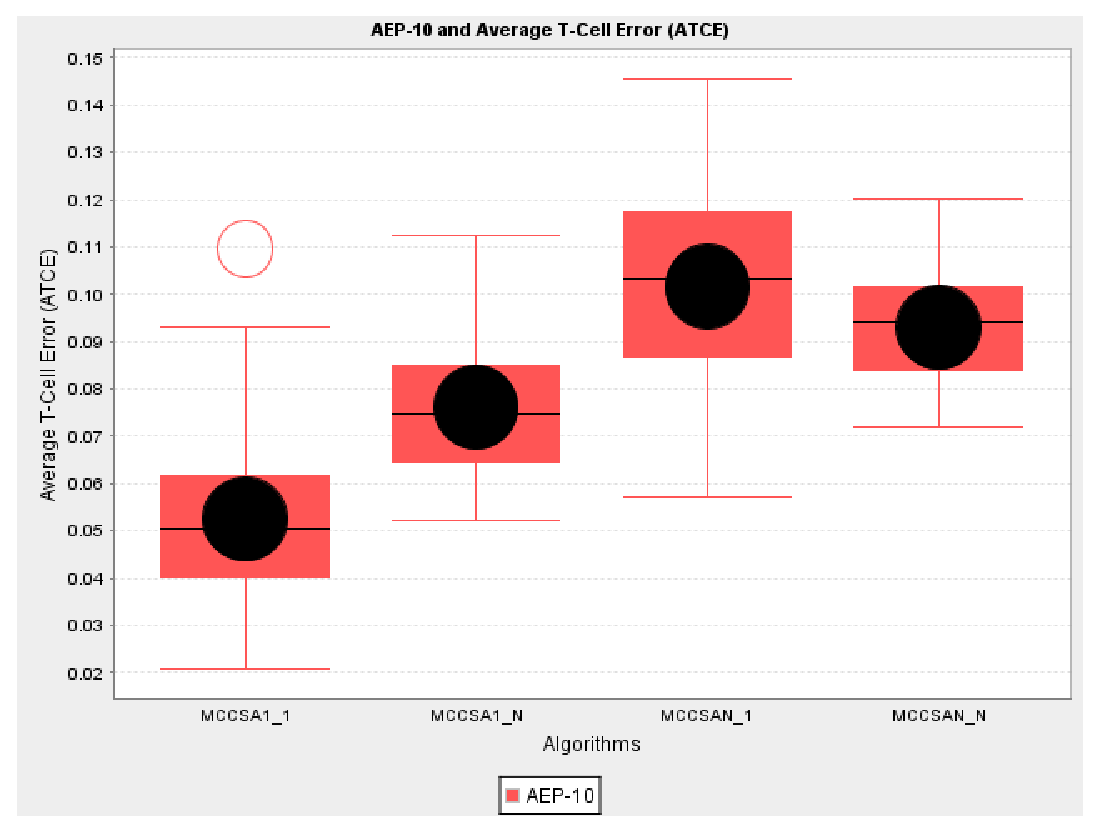
\includegraphics[scale=0.40]{Cells/MCCSA-relationships-ATCE}
	% new line for second set
	\end{minipage}}\\
	\subfloat[Response Error on ACSP-10.]{
	\label{fig:cells:mccsa:study2:re:boxplot} %% label 
	\begin{minipage}[t]{\textwidth}
		\centering 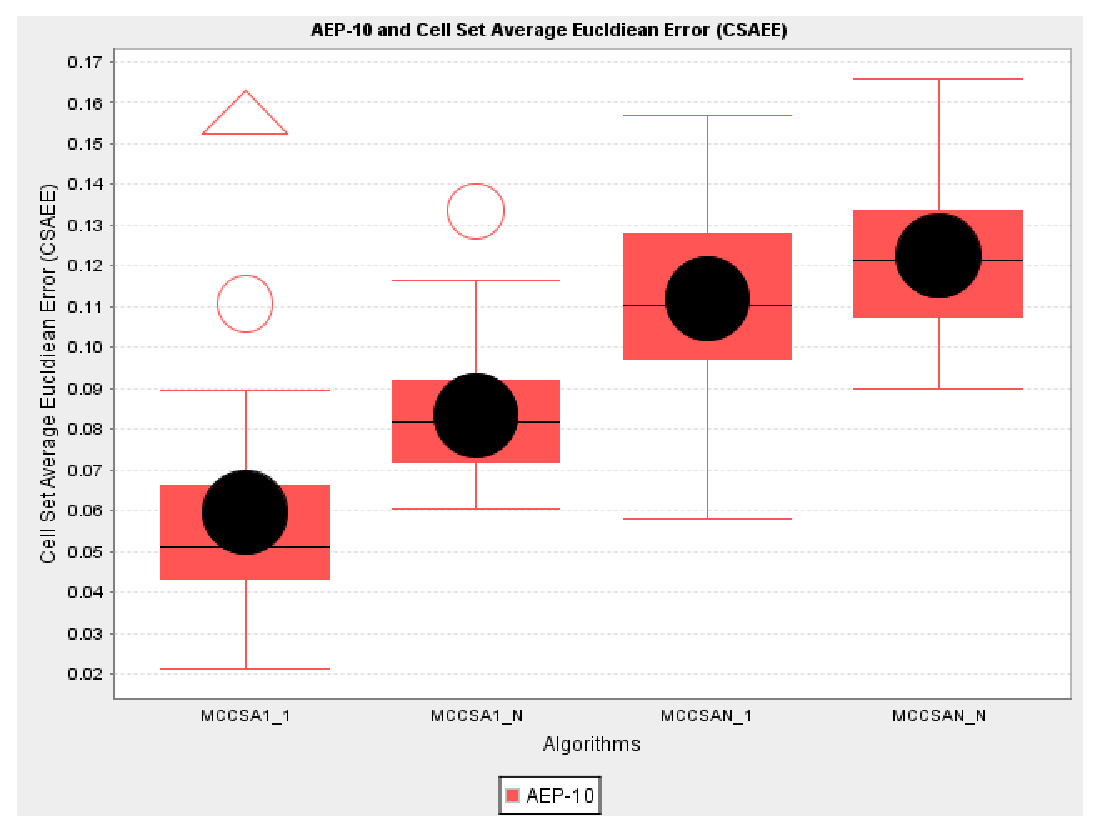
\includegraphics[scale=0.40]{Cells/MCCSA-relationships-RE}
	\end{minipage}}%	
	\caption{Box-and-whisker plot's for the relationship configuration with ECCSA.}
	\label{fig:cells:mccsa:all:boxplot} %% label for entire figure
\end{figure}


% plots of the relationships
\begin{figure}[htp]
	\subfloat[MCCSA(1-1).]{
	\label{fig:cells:mccsa:relationships:a} %% label 
	\begin{minipage}[t]{0.50\textwidth}
		\centering 
\includegraphics[scale=0.45]{Cells/MCCSA-1-1}
	\end{minipage}}%
	\hfill
	\subfloat[MCCSA(1-N).]{
	\label{fig:cells:mccsa:relationships:b} %% label 
	\begin{minipage}[t]{0.50\textwidth}
		\centering 
\includegraphics[scale=0.45]{Cells/MCCSA-1-N}
	\end{minipage}}\\
	% new line for second set	
	\subfloat[MCCSA(N-1).]{
	\label{fig:cells:mccsa:relationships:c} %% label 
	\begin{minipage}[t]{0.50\textwidth}
		\centering 
\includegraphics[scale=0.45]{Cells/MCCSA-N-1}
	\end{minipage}}%
	\hfill
	\subfloat[MCCSA(N-N).]{
	\label{fig:cells:mccsa:relationships:d} %% label 
	\begin{minipage}[t]{0.50\textwidth}
		\centering \includegraphics[scale=0.45]{Cells/MCCSA-N-N}
	\end{minipage}}
	% end
	\caption{Example plots of the B- (top of each plot) and T-Cell (bottom of each plot) repertoires from the MCCSA at the end of the run on ACSP-10 for all four inter-relationship types.}
	\label{fig:cells:mccsa:relationships:plots} %% label for entire figure
\end{figure}


%
% Analysis
%
\subsubsection{Analysis}
This section provides an analysis of the results reported in the previous section in the context of the goals of the empirical study. 

%
% Mapping Trends
%
\paragraph{Mapping Trends}
% section
This section considers the effects of using the Euclidean and Hamming antigen-dependant inter-repertoire schemes. 
% B-cells
The B-cell diversity and error show no significant difference between the mapping schemes. This is an expected result, as the mapping scheme and the chosen ECCSA does not effect the B-cell repertoire.
% T-cells
The T-cells showed a small decrease in diversity with the Hamming mapping, and more critically showed a factor of 10 increase in Average T-cell Error compared to the Euclidean mapping. This difference in error was reflected more strongly in the Response Error that showed a an increase in error of $\approx70$. 
% plots
The example plots in Figure~\ref{fig:cells:mccsa:study1:plots} clearly show well organised B-cell repertoires under both mapping schemes as expected, and the clear organisation and disorganisation in the T-cell repertoires between the Euclidean and Hamming schemes respectively.
% trends
These results demonstrate that under the circumstances investigated, that Hamming distance is not a sufficient approximation for Euclidean distance, not providing enough information to promote the same structures in the T-cell repertoire as were selected in the B-cell repertoire. These results demonstrate the fragility of proxy-based response to the antigen-centric mapping function. 

%
% Inter-Repertoire Relationship Trends
%
\paragraph{Inter-Repertoire Relationship Trends}
% section
This section considers the mapping relationships between the number of selected (stimulating) cells in each repertoire.
% b-cells and t-cells
The diversity and error of the B-cell repertoire increased with the number of selected B-cells. This same general behaviour was observed with the T-cell diversity and the number of selected T-cells. The ATCE increased with the number of selected T-cells with 1 triggering B-cell, although showed a small decrease with the increase in selected T-cells with $N$ selected T-cells.
% mapping
The average B-cell to T-cell mapping error showed an increase in the number of selected T-cells with both 1 and $N$ selected B-cells, and effect also observed with the mapping error of the selected T-cell set. 
% trend
Together these observations suggest that the selection of a single cell and integration of its clones results in a more specialised (lower diversity and error) repertoire and mapping. Conversely, the result suggests that the selection of a large activated set and integration of a few clones from each results in a more diverse cellular perspective on the cellular and/or antigenic trigger. 
% interpretation
This observation lends support to the \emph{oligoclonal axiom} of the clonal selection strategy outlined in Section~\ref{subsec:cells:paradigm:clonalselection}. More specifically, in the context of the replacement-based resource allocation scheme used in the assessed algorithms, selection and integration of few cells with many clones results in a more specific and less diverse repertoire. This finding in the context of the bi-repertoire model with antigenic and cellular triggers lends support to the same finding in Section~\ref{sec:cells:ccsa:rcsa}.
% error
This trend is observed poignantly in the Response Error from the relationship results where the 1-1 configuration achieved the lowest response-by-proxy error, increasing with the number of selected T-cells and selected B-cells. The plots in Figure~\ref{fig:cells:mccsa:relationships:plots} depict this in the organisation of the B-cell and T-cell repertoires in those configurations where a single cell is selected by antigen or cellular trigger resulting in the integration of a set of clonal siblings (1-1, 1-$N$, and $N$-1).


%
% Conclusions
%
\subsubsection{Conclusions}
This section summarises the findings of the empirical study into the Mediated Cellular Clonal Selection Algorithm in terms of the primitives that were the focus of the study and the expectations that motivated the study.

\begin{enumerate}
	% mappings
	\item \emph{Mappings}
	\begin{enumerate}		
			\item An antigen-centric mapping scheme results in the effective blind promotion (specialisation) of the T-cell repertoire and proxied response.
		\item The quality of the mapping with regard to proxied responses in mediated clonal selection is as good as the amount of antigen-centric information mapped between the repertoires. 
		\item The remapping of the antigen-assessment Euclidean distance resulted in an effective proxy response, whereas the approximation of the assessment in the Hamming distance resulted in a markedly unsuccessful proxied response.
	\end{enumerate}
	
	% relationships
	\item \emph{Relationships}
	\begin{enumerate}
		\item The number of activated B-cells and thus stimulus for the T-cell repertoire was an important factor in response capability, resulting in a specialisation of feature detectors for remapping.
		\item The one-to-one and one-to-many relationship configurations between the repertoires resulted in the better proxied responses, with more than a factor of two decrease in capability with an increase in the number of selected B-cells.
		\item One-to-Many selection and clonal integration for a given repertoire results in improved repertoire capability (lower error), increase repertories organisation (lower diversity), and an improved mapping given the specialisation it provides to the adaptive process.
	\end{enumerate}	
\end{enumerate}



%
% Cell-Cell Recognition
%
\section{Cell-Cell Recognition}
\label{sec:cells:network}
This section elaborates on clonal selection by introducing a pattern recognition interpretation of the Immune Network Theory and its integration into the cellular clonal selection framework.


%
% Network Clonal Selection}
%
\subsection{Network Clonal Selection}
\label{sec:cells:network:theory}
% metaphor
The Idiotypic Network Theory proposed by Jerne indicates that receptors (free or surface bound antibody) are selected by other receptors in addition to antigen (Section~\ref{subsec:background:negativeselection}). As such, one may define two additional types of receptor-to-receptor interaction in additional to conventional interaction with antigen: (1) The activation of a receptor by the idiotype of another receptor that results in the creation of more anti-receptor receptors, (2) The activation of a receptor that is specialised toward an antigen by another receptor that results in the creation of more receptors for the antigen without the presence of the antigen and anti-idiotype receptors for the triggering receptor. The theory suggests that the aggregation of these low-level behaviours results in a network of receptors that may interact with antigen and each other providing both an antigen-recognition system and the self-regulation of immune response. 


%
% Recognition and Relationships
%
\subsubsection{Recognition and Relationships}
The two direct receptor relationships include: \emph{Receptor-Antigen}: the traditional relationship where receptors for the antigen (target) are created with minor variations toward improving recognition, and \emph{Receptor-Receptor}: the the idiotypic relationship where receptors for the triggering receptor (target) are created (anti-receptor receptors) with minor variations toward improving recognition. Both of these cases provide examples of \emph{direct relationships}, that of a receptor and an antigen or a receptor and another receptor. In the first case, receptors have an \emph{implicit relationship} with other receptors that also match for the same antigen in that they compete with each other for selection by the antigen. The second case is a lot more interesting, given the recurrent relationships that may result. These relationships are considered in the context of how a given receptor came to be, assuming a single matching source is responsible for receptor maturation. For example, a receptor may match to another receptor that has been matured for an antigen. Therefore, there is a direct relationship between the first receptor and the second, as well as a \emph{proportional relationship} between the first receptor and the second receptors antigen (for example of both relationships see Figure~\ref{pic:cells:network:relationships:examples}). 

\begin{figure}[htp]
	\subfloat[Proportional Relationship.]{
	\label{pic:cells:network:relationships:examples:proportional} %% label for first subfigure
	\begin{minipage}[c]{0.5\linewidth}
		\centering \includegraphics[scale=0.85]{Cells/network-relationships-proportional}
	\end{minipage}}%
	\hfill
	\subfloat[Implicit Relationship.]{
	\label{pic:cells:network:relationships:examples:implicit} %% label for second subfigure
	\begin{minipage}[c]{0.5\linewidth}
		\centering \includegraphics[scale=0.85]{Cells/network-relationship-implicit}
	\end{minipage}}
	\caption{Examples of more complex relationships that may be formed given receptor-receptor recognition.}
	\label{pic:cells:network:relationships:examples} %% label for entire figure
\end{figure}

%
% Matching Function
%
\subsubsection{Matching Function}
The clonal selection algorithm results in a repertoire that directly (relationship-wise) models features of the input space. When receptors themselves are treated as input signals a variety of representations may be used in the matching. The network theory proposes that receptors match onto a part of the receptor that is distinct for receptors of that lineage, although different from the receptors combining region (part of the other receptor that does the binding). A natural implementation scheme is to assign a random or remapping of the primary bit string to each \naive\ receptor that, like the primary string, is inherited and maturated by progeny cells. This results in the co-evolution (co-adaptation) of the primary string for activation and the secondary string for secondary effects (for example, see Figure~\ref{pic:cells:network:representation}).

\begin{figure}[ht]
	\centering
	\includegraphics[scale=0.85]{Cells/network-mapping-representation}
	\caption{Depiction of the two-string representation scheme.}
	\label{pic:cells:network:representation}
\end{figure}

A natural representation (using the same string for both) will likely result in a positive feedback system, where the exposed antigen will be amplified by repeated simulated exposures. Any regularity of the antigenic pattern that is provided on the secondary strings (such as sub-strings or reordering) will likely have this amplification effect, proportional to the fidelity of the mapping of the regularity. This amplification of input signal may be useful to reinforce the acquisition of knowledge. A natural representation will continue to promote the same instigating signal for as long as activated members are promoted to antigen-like status.

%
% Higher-Order Structures
%
\subsubsection{Higher-Order Structures}
A steady-state application of the approach emphasises some important properties regarding the formation of relationships as networks (graphs) of activation and exposure. In this interpretation, an antigen matches onto and activates a single receptor. The activated receptor is copied from the repertoire and is provided as an input signal in the next cycle. In this next cycle, both an antigen and the previously activated receptor are offered as input signals to the repertoire. A queue-based exposure scheme is used such that the more-recent activated receptors (instigation of relationship) are admitted, and older receptors are discarded. Therefore, the previously activated receptor is discarded, and the newly antigenic-activated cell is promoted to the next cycle as an input signal. The behaviour of this scheme may be described with an example (see Figure~\ref{pic:cells:network:recurrent} and Table~\ref{tab:cells:network:activationscheme}).

\begin{figure}[ht]
	\centering
	\includegraphics[scale=0.85]{Cells/network-structures-feedback}
	\caption{Example of a simple two-receptor promotion scheme.}
	\label{pic:cells:network:recurrent}
\end{figure}

\begin{table}[ht]
	\centering\small
		\begin{tabular}{lll}
		\toprule
		\textbf{Cycle} & \textbf{Exposed} & \textbf{Activated} \\ 
		\toprule
		$1$ & A1 & R1 \\ 
		\midrule
		$2$ & A2, R1 & R2, R1a \\ 
		\midrule
		$3$ & A3, R2 & R3, R2a  \\ 
		\midrule
		$4$ & A4, R3 & R4, R3a \\ 
		\midrule
		$t$ & $A_t$, $R_{t-1}$ & $R_t$, $R_{t-1}a$ \\ 
		\bottomrule
		\end{tabular}	
	\caption{Exposure-activation scheme for a minimal implementation.}
	\label{tab:cells:network:activationscheme}
\end{table}

If a natural mapping is used for $string2$, then the scheme provides a simple signal-reinforcement scheme that provides a linear amplification ($t-1$) reinforcement of signals past. If a remapping scheme is used for $string2$ (such as a random string), then the scheme provides new information in subsequent exposures that may result in the formation of a connection between two different input signals. The simplest example is the selection of $R1a$ by $A2$. In a natural mapping, if $A2$ selected $R1a$ then $A1$ and $A2$ would be the same input signal, and $R1$ and $R1a$ are likely the same receptor or clonal siblings (same ancestor). In a remapping scheme (such as random), it is possible for the remapped string to match for a receptor that is also matched for by an antigen (see Figure~\ref{pic:cells:network:remapping}). 

\begin{figure}[ht]
	\centering
	\includegraphics[scale=0.85]{Cells/network-remapping-schemes}
	\caption{Depiction of the example difference between a natural and remapping scheme.}
	\label{pic:cells:network:remapping}
\end{figure}

The remapping example provides an example of a relationship that may form between two different antigen ($A1$ and $A2$), facilitated by the remapping of receptors using the two-string scheme. If $A2$ is withdrawn, the relationship is fostered by $A1$, which activates $R1$, which in turn activates $R1a$. If $A2$ is withdrawn for all time, then the relationship will deteriorate due to genetic drift\footnote{The relationship is fostered by activation (usefulness), although here genetic drift refers to the adaptation of receptors (their progeny) in response to activation.}, thus $A2$ provides a correcting influence to the relationship. If $A1$ is withdrawn then the other half of the relationship is reinforced ($R1a$), and again if $A1$ is not returned, then $R1a$ may drift such that R1 does not match to it any longer. The example relationship is unidirectional, in that the primary string of $R1a$ is a generalisation of $A2$ and $R1$'s secondary string. A natural extension is to consider the implications of $R1a$'s secondary string. If $R1a$ matches for $R1$ then both $R1$ and $R1a$ provides surrogates for $A1$ and $A2$ reinforcing each other and the repertoires relationship between $A1$ and $A2$. It requires that $R1$'s primary string is a generalisation of $A1$ and $R1$'s secondary string. This network may be depicted as follows ($R1a$ is renamed $R2$).

\begin{figure}[ht]
	\centering
	\includegraphics{Cells/network-remapped-example}
	\caption{Depiction of the relationship between remapped antigen and receptors ($ps$ is primary and $ss$ is secondary string).}
	\label{pic:cells:network:remappingspecific}
\end{figure}

A larger queue allows more intra-antigen relationships (larger relationship structures in general), which in turn may prolong the activation of structures, but does not facilitate perpetual (antigen-independent) structure formation. Therefore, \emph{Structure Durability} is defined when the exposure set size defines the sustainability of a structure in active memory (essentially defining short-term memory), in the absence of renewed promotion. Finally, the examples do not take into account the proliferation of selected receptors, therefore the density concerns were subsumed with activation counts that delineated receptor persistence. Additionally, in the structures proposed the secondary strings become surrogates for antigen strings, thus `take the form' of antigen signals. This suggests that a mapping, such as substring's or reordering of the primary string may be easier for the system to retrofit for such a purpose rather than a random-based mapping (assuming similarity rather than complementarity of the mapping between receptors and antigen).

%
% Recurrent Empirical Study
%
\subsection{Recurrent Empirical Study}
\label{sec:cells:network:recurrent:study}
%
% Aim
%
\subsubsection{Aim}
The aim of this empirical study is to investigate some of the primiting behaviours of the cellular clonal selection strategy with intra-repertoire (network) interactions, specifically the recurrent network model. Toward this end, the study had the following motivating goals:

\begin{enumerate}	
	\item Investigate the effects on the composition and capability of the repertoire under recurrent cellular exposures.
	\item Assess a variety of cell promotion pressures in the recurrent network model.
\end{enumerate}

%
% Method
%
\subsubsection{Method}

%
% Problems
%
\paragraph{Problems}
This study used the ACSP-10 problem used for the CCSA empirical study in Section~\ref{sec:cells:ccsa:ccsa}.

%
% Algorithms
%
\paragraph{Algorithms}
Algorithm~\ref{alg:cells:nccsa:recurrent} defines the recurrent variation of the Network Cellular Clonal Selection Algorithm. Like ECCSA, two exposures occur each epoch, although unlike ECCSA both exposures occur to the same repertoire of cells. The second exposure involves the exposure of the Best Matching Cell (BMC) from the last \emph{antigen} exposure ($BMC_{t-1}$) to the repertoire. A cellular exposure involves the assessment of the repertoire against the representation in the cell, specifically using the Euclidean affinity function between the representation as is used between an antigen and a cell (defined in Equation~\ref{eq:cells:realised:euclidean}).

\begin{algorithm}[htp]
  \SetLine
  \SetKwData{Tissue}{T}
  \SetKwData{Antigen}{A}
  \SetKwFunction{Exposure}{Exposure}
  \KwIn{\Antigen, \Tissue, $BMC_{t-1}$, $N_{selection}$, $N_{clones}$, $P_{mutation}$}
	\KwOut{$T_{rs}$}	
	
	% expose to the antigen
	$T_{rs} \leftarrow$ \Exposure{\Antigen, \Tissue, $N_{selection}$, $N_{clones}$, $P_{mutation}$}\;		
	% expose to the last bmu
	\Exposure{$BMC_{t-1}$, \Tissue, $N_{selection}$, $N_{clones}$, $P_{mutation}$}\;	
	% return it	
	\Return{$T_{rs}$}\;
	
	\caption{Recurrent Network Cellular Clonal Selection.}
	\label{alg:cells:nccsa:recurrent}
\end{algorithm}	

% natural mapping
A Natural Mapping variation of the approach was assessed to provide a baseline of performance referred to as RE-NCCSA-NM. The algorithm responded to each exposure using the replacement mechanisms of RCCSA, and used the following configuration: $N_{cells}=100$, $N_{selected}=1$, and $N_{clones}=5$, assigning 5\% of the repertoire per exposed stimulus. This approach was called natural mapping, because indeed no mapping was used, where $BMC_{t-1}$ were exposed directly to the repertoire, likely causing their clonal siblings in the repertoire to respond.
% remapped
A remapping approach was used where each cell was provided with two data strings: a primary string which responded to exposed stimuli, and a secondary string which may be used as an antigenic stimulus (the two-string method described in Section~\ref{sec:cells:network:theory}).
% configuration
Table~\ref{tab:network:nccsa:renccsa} defines a set of four different \emph{replacement-based} promotion schemes used with the mapping variation of the algorithm. The schemes are replacement based in that the configurations define the specific pressures applied during the competition for limited position in the repertoire during the integration of clones. \emph{Similarity} refers to the specific representation of cells (primary or secondary) used to match clones with cells in the repertoire, and \emph{Assessment} refers to the affinity scoring (against the primary or secondary string) used during the tournament for the position in the repertoire between a clone and its most similar counterpart in the repertoire.
% expectations
The promotion of the antigen in the secondary representation is expected to promote similar cells in the recurrent exposure. The promotion of the cellular stimulus in the primary representation in the cellular exposure is expected to improve the mapping in the recurrent exposure. 

\begin{table}[htp]
	\centering\small
		\begin{tabular}{lllll}
		\toprule
		\textbf{R-NCCSA} & \multicolumn{2}{c}{\textbf{Antigen Exposure}} & \multicolumn{2}{c}{\textbf{Cellular Exposure}} \\ 
		\midrule
		\emph{Name} & \emph{Assessment} & \emph{Similarity} & \emph{Assessment} & \emph{Similarity} \\ 
		\toprule
		\emph{PP} & Primary  & Primary  & Primary  & Primary  \\ 
		\emph{PS} & Primary  & Primary  & Secondary & Secondary \\ 
		\emph{SS} & Secondary & Secondary & Secondary & Secondary \\ 
		\emph{SP} & Secondary & Secondary & Primary  & Primary  \\ 
		\bottomrule
		\end{tabular}
	\caption{Summary of the various replacement configurations for the mapped Recurrent Exposure Network Cellular Clonal Selection Algorithm (RE-NCCSA).}
	\label{tab:network:nccsa:renccsa}
\end{table}


%
% Experiment
%
\paragraph{Experiment}
This study used the same general experimental configuration including stop conditions as were used for the CCSA empirical study in Section~\ref{sec:cells:ccsa:ccsa}. 
% new measures
Two additional diversity measures were introduced to assess the composition of the repertoire with regard to secondary mappings. The Average Cell Mapped Diversity (ACMD) assesses the average Hamming distance of a given cell to all the other cells in the repertoire with regard to the secondary representation. The Average Network Cell Diversity (ANCD) provided a similar diversity measure although treats both representations of a given cell as one providing an indication of the composition of the repertoire independent of representations. Both diversity measures use the same mechanism as ACD in Equation~\ref{eq:cells:realisation:acd} on their representations respectively. Finally, a measure was introduced to assess the state of the mappings between the repertoire and recurrent cellular exposures called the Average Mapped Best Matching Cell Error (AMBMCE), that averaged the Euclidean distance between recurrent cells secondary representation and the BMC in the repertoire for each epoch using the same mechanism as ACE in Equation~\ref{eq:cells:realisation:measure:ace}.

%
% Results
%
\subsubsection{Results}
% tables
Table~\ref{tab:network:nccsa:rnccsa:results} provide a summary of results for each algorithm-problem combination including the mean ($\bar{x}$) and standard deviation ($\sigma$) of collected measure values. The non-parametric Mann-Whitney~U statistical test was calculated pair-wise for all algorithms. 
% graphs
Figures \ref{fig:cells:network:rnccsa:ace:boxplot}, \ref{fig:cells:network:rnccsa:acd:boxplot}, \ref{fig:cells:network:rnccsa:ambmue:boxplot} show the ACE, ACD, and AMBMCE respectively. 
% plots
Figure~\ref{fig:cells:nccsa:rnccsa:plots} provide example plots of the response mapping and final repertoire. Results from all example plots are taken from the end of the run with algorithm and problem configurations matching those used during experimentation, and a random number generator seed of 1 and 5 for the algorithm and problem respectively.

\begin{table}[htp]
	\centering\small
		\begin{minipage}{\textwidth}
		\begin{tabular}{lllllllllll}
		\toprule
		\textbf{System} & \multicolumn{2}{c}{\textbf{ACD}} & \multicolumn{2}{c}{\textbf{ACE}} & \multicolumn{2}{c}{\textbf{ACMD}} & \multicolumn{2}{c}{\textbf{ANCD}} & \multicolumn{2}{c}{\textbf{AMBMCE}}\\
		\midrule
		\emph{NCCSA} & $\bar{x}$ & $\sigma$ & $\bar{x}$ & $\sigma$ & $\bar{x}$ & $\sigma$ & $\bar{x}$ & $\sigma$ & $\bar{x}$ & $\sigma$\\
		\toprule
		NM & 93.218 & 0.248 & 0.019 & 0.011 & N/A & N/A & N/A & N/A & 0 & 0 \\
		PP & 91.974 & 0.413 & 0.09 & 0.025 & 91.777 & 0.46 & 183.751 & 0.669 & 0.184 & 0.026 \\
		PS & 91.912 & 0.31 & 0.03 & 0.013 & 92.032 & 0.453 & 183.944 & 0.597 & 0.173 & 0.025 \\
		SS & 91.805 & 0.429 & 0.211 & 0.04 & 91.783 & 0.419 & 183.588 & 0.609 & 0.147 & 0.034 \\
		SP & 91.744 & 0.421 & 0.234 & 0.039 & 91.745 & 0.403 & 183.489 & 0.542 & 0.162 & 0.03 \\
		\emph{Sign.} & True &  & True &  & True\footnote{False for RNCCSA-PP and RNCCSA-SS, RNCCSA-PP and RNCCSA-SP, RNCCSA-SS and RNCCSA-SP} &  & True\footnote{False for RNCCSA-PP and RNCCSA-PS, RNCCSA-PP and RNCCSA-SS, RNCCSA-PP and RNCCSA-SP, RNCCSA-SS and RNCCSA-SP} &  & True\footnote{False for RNCCSA-PP and RNCCSA-PS, RNCCSA-PS and RNCCSA-SP, RNCCSA-SS and RNCCSA-SP} & \\
		\bottomrule
		\end{tabular}	
		\end{minipage}
	\caption{Summary of results for Recurrent Network Cellular Clonal Selection Algorithm (R-NCCAS) on ACSP-10}
	\label{tab:network:nccsa:rnccsa:results}
\end{table}

% graphs
\begin{figure}[htp]
	\subfloat[Average Cell Error on ACSP-10.]{
	\label{fig:cells:network:rnccsa:ace:boxplot} %% label 
	\begin{minipage}[t]{0.50\textwidth}
		\centering \includegraphics[scale=0.41]{Cells/RNCCSA-ACE-plot}
	\end{minipage}}%
	\hfill
	\subfloat[Average Cell Diversity on ACSP-10.]{
	\label{fig:cells:network:rnccsa:acd:boxplot} %% label 
	\begin{minipage}[t]{0.50\textwidth}
		\centering \includegraphics[scale=0.41]{Cells/RNCCAS-ACD-plot}
	\end{minipage}}\\
	%\hfill
	\subfloat[ Average Mapped BMC Error on ACSP-10.]{
	\label{fig:cells:network:rnccsa:ambmue:boxplot} %% label 
	\begin{minipage}[t]{\textwidth}
		\centering \includegraphics[scale=0.41]{Cells/RNCCSA-AMBMUE-plot}
	\end{minipage}}%
	\caption{Box-and-whisker plot's from the Recurrent NCCSA Empirical Study.}
	\label{fig:cells:nccsa::study1:all:boxplot} %% label for entire figure
\end{figure}


% plots of PS
\begin{figure}[htp]
	\subfloat[Response Mapping plot for R-NCCSA-PS, shows $A$, $BMC_{t1}a$, $BMC_{t-1}$, $BMC_{t1}b$ from left to right, for an epoch.]{
	\label{fig:cells:nccsa:rnccsa:a} %% label 
	\begin{minipage}[t]{0.45\textwidth}
		\centering \includegraphics[scale=0.45]{Cells/RNCCSA-PS-map-plot}
	\end{minipage}}%
	\hfill
	\subfloat[Repertoire plot for R-NCCSA-PS, shows primary and secondary representations and antigen from left to right.]{
	\label{fig:cells:nccsa:rnccsa:b} %% label 
	\begin{minipage}[t]{0.45\textwidth}
		\centering \includegraphics[scale=0.45]{Cells/RNCCSA-PS-rep-plot}
	\end{minipage}}\\
	% end
	\caption{Example plots from of the response mappings and final repertoire from R-NCCSA-PS on ACSP-10.}
	\label{fig:cells:nccsa:rnccsa:plots} %% label for entire figure
\end{figure}


%
% Analysis
%
\subsubsection{Analysis}
This section provides an analysis of the results reported in the previous section in the context of the goals of the empirical study. 

%
% Promotion Trends
%
\paragraph{Promotion Trends}
% this section
This section considers the results of the recurrent network algorithm in the context of the trends for the different promotion schemes.
% generally
The natural mapping achieved the best results with regard to ACE as expected, showing a AMBMCE of zero suggesting that cells mapped onto themselves or clonal siblings with no error on average by the end of the run, providing an ideal (in the mapping sense) case for comparison.
% diversity
The various promotion schemes for the mapped recurrent algorithm showed little comparative difference between the three diversity scores: ACD, ACMD, and ANCD. The ACD scores showed a slight decrease with the remapping approaches compared to the natural mapping. The similarity between ACD and ACMD scores suggests that organisation of the information in the primary and secondary representations (pseudo-repertoires) was generally equivalent across the promotion schemes.
% ACE
The telling results were provided in the error measures. The two promotion schemes that promoted the primary representation achieved a much lower ACE as expected than those that promoted the secondary representation against the antigen. Interestingly the configuration that promoted the secondary representation against the cellular exposure (PS) performed better than the promotion of the primary string on both exposures (PP). 
% AMBMCE
The error results for the recurrent cellular exposures were poor compared to error scores for viable ACSP ($<0.1$), where the promotion of the secondary string against antigen exposures resulted in relatively lower AMBMCE than the promotion of the primary string. 
% observation
A general observation of the state of the repertoire and exposure mappings during the execution of general runs reviled that consistent intra-repertoire mappings were unstable across the various promotion schemes (for example see Figure~\ref{fig:cells:nccsa:rnccsa:plots}). This is reflected in the poor mapping error scores achieved.

%
% Curtailing Instability
%
\paragraph{Curtailing Instability}
The complexity of the approach makes analysis difficult although the observed behaviour may be explained by the instability of the general approach. This instability is likely the result of the competition between similar representations for antigen and for cells. For example in the case of PP, the promotion of primary strings in the cellular exposure may be considered the promotion of random secondary strings, with no explicit pressure of adding meaning to the secondary strings of antigen-selected BMC's. This is addressed in PS by the cyclic promotion of secondary strings which are expected to provide pattern-matching loops which counter some of the instability effective ACE.
% conflicting
The results for secondary string promotion during antigen exposures suggest that the promotion of BMC's for antigen in the repertoire via proxy (t+1 cellular exposure), in particular R-NCCSA-SP, is insufficient for the repertoire to address the ACSP. This suggests that the de-coupled promotion of antigen-BMC within the repertoire may result in conflicting competition between primary and secondary representations.

%
% Conclusions
%
\subsubsection{Conclusions}
This section summarises the findings of the empirical study into the Recurrent Network Cellular Clonal Selection Algorithm in terms of the primitives that were the focus of the study and the expectations that motivated the study.

\begin{enumerate}
	% primitives
	\item \emph{Primitives}
		\begin{enumerate}
			\item The Recurrent NCCSA provides a viable approach for investigating the subtle effects of intra-repertoire remapping of exposure signals and the subtleties of competition in such a mapping.
		\end{enumerate}
		
	% behaviours
	\item \emph{Behaviours}
	\begin{enumerate}
		\item The recurrent exposure of cells via a natural mapping provides a reinforcement of antigenic signals
		\item The recurrent exposure of remapped cells requires careful consideration of the competition between representations to avoid conflicts in such competition.
	\end{enumerate}	
\end{enumerate}


%
% Dual Exposure Empirical Study
%
\subsection{Dual Exposure Empirical Study}
\label{sec:cells:network:dualexposure:study}
%
% Aim
%
\subsubsection{Aim}
The aim of this study is to investigate the antigen-driven formation of intra-repertoire structures as outlined in Section~\ref{sec:cells:network:theory}, and Figures \ref{pic:cells:network:remappingspecific} and \ref{pic:cells:network:remappingspecific}. Specifically, this empirical study is concerned with further investigating the subtle application of replacement pressure as was considered in the recurrent model, although toward the formation and promotion of antigen-dependant rather than cellular-dependant structures. Toward this end, this study has the following goals:

\begin{enumerate}
	\item Assess the composition and capability of the repertoire under a dual-exposure model.
	\item Investigate the formation of antigen-dependant high-order structures via the application of intra-repertoire promotion schemes.
\end{enumerate}


%
% Method
%
\subsubsection{Method}

%
% Problems
%
\paragraph{Problems}
This study used the ACSP-10 problem used for the CCSA empirical study in Section~\ref{sec:cells:ccsa:ccsa}.

%
% Algorithms
%
\paragraph{Algorithms}
Dual exposure refers to the way in which the repertoire interacts with the antigen, specifically two at a time (requiring the ACSP to be comprised of an even number of CSP). Dual exposure may be considered a variation on the linear Cellular Exposure Regime considered in Algorithm~\ref{alg:cells:realisation:exposure:aep:cer} where the first antigen in the pair is always exposed to the repertoires primary string representation, and the second antigen to the secondary string representation (see Algorithm~\ref{alg:cells:nccsa:dual}). Such exposure governs the selection of the BMC returned as a response from the repertoire to satisfy the requirement of the exposure represented. 

\begin{algorithm}[htp]
  \SetLine  
  \SetKwFunction{Exposure}{Exposure}
  \SetKwData{Tissue}{T}
  
  \KwIn{$A_1$, $A_2$, \Tissue, $N_{selection}$, $N_{clones}$, $P_{mutation}$}
	\KwOut{$T_{rs}$}	
	
	% primary exposure
	$T_{rs} \leftarrow$ \Exposure{$A_1$, \Tissue, $N_{selection}$, $N_{clones}$, $P_{mutation}$}\;		
	% secondary exposures
	$T_{rs} \leftarrow$ \Exposure{$A_2$, \Tissue, $N_{selection}$, $N_{clones}$, $P_{mutation}$}\;		
	% return it	
	\Return{$T_{rs}$}\;
	\caption{Dual Exposure Network Cellular Clonal Selection.}
	\label{alg:cells:nccsa:dual}	
\end{algorithm}	

As with the recurrent approach (defined in Algorithm~\ref{alg:cells:nccsa:recurrent}) a series of configuration schemes are considered that provide subtle adjustments to the replacement competition of aggregated clonal sets against the repertoire. Unlike the recurrent approach, these configurations are concerned with the effects of varying or decoupling the context for similarity and assessment used during replacement (see Table~\ref{tab:network:nccsa:denccsa:configuration}). In this case, \emph{Similarity} refers to the string representation (primary or secondary) used to locate the most similar repertoire member for a clone to compete with, and \emph{Assessment} refers to which antigen the representation is assessed against (primary antigen or secondary antigen). As mentioned, the first exposure is always assessed against the primary representation, and the second against the secondary representation.

\begin{table}[htp]
	\centering\small
		\begin{tabular}{lllll}
		\toprule
		\textbf{DE-NCCSA} & \multicolumn{2}{c}{\textbf{First Exposure}} & \multicolumn{2}{c}{\textbf{Second Exposure}} \\ 
		\midrule
		\emph{Name} & \emph{Assessment} & \emph{Similarity} & \emph{Assessment} & \emph{Similarity} \\ 
		\toprule
		\emph{PP-SS} & Primary & Primary & Secondary & Secondary \\ 
		\emph{PS-SP} & Primary & Secondary & Secondary & Primary \\				
		\emph{SS-PP} & Secondary & Secondary & Primary & Primary \\		
		\emph{SP-PS} & Secondary & Primary & Primary & Secondary \\						
		\bottomrule
		\end{tabular}
	\caption{Summary of the various replacement configurations for the Dual Exposure Network Cellular Clonal Selection Algorithm (DE-NCCSA).}
	\label{tab:network:nccsa:denccsa:configuration}
\end{table}


%
% Experiment
%
\paragraph{Experiment}
This study used the same general experimental configuration including stop conditions as were used for the R-NCCSA empirical study in Section~\ref{sec:cells:network:recurrent:study}. 

%
% Results
%
\subsubsection{Results}
% tables
Table~\ref{tab:network:nccsa:denccsa:results} provide a summary of results for each algorithm-problem combination including the mean ($\bar{x}$) and standard deviation ($\sigma$) of collected measure values. The non-parametric Mann-Whitney~U statistical test was calculated pair-wise for all algorithms. 
% graphs
Figure~\ref{fig:cells:network:denccsa:ace:boxplot} shows the Average Cell Error (ACE) for the four different dual exposure configurations. 
% plots
Figure~\ref{fig:cells:nccsa:denccsa:plots} provides example plots of the four schemes at the end of a run on ACSP-2. The algorithms and problem use a random number generator seed of 1 and 4 respectively. The configuration of each algorithm was reduced to $N_{cells}=20$ to ensure a proportional distribution of cells in the repertoire. The smaller ACSP-2 was chosen to clearly highlight the formation and/or lack of formation of bi-antigen structures in the primary and secondary representations.

\begin{table}[htp]
	\centering\small
		\begin{minipage}{0.80\textwidth}
		\centering
		\begin{tabular}{lllllllll}
		\toprule
		\textbf{System} & \multicolumn{2}{c}{\textbf{ACD}} & \multicolumn{2}{c}{\textbf{ACE}} & \multicolumn{2}{c}{\textbf{ACMD}} & \multicolumn{2}{c}{\textbf{ANCD}}\\
		\midrule
		\emph{NCCSA} & $\bar{x}$ & $\sigma$ & $\bar{x}$ & $\sigma$ & $\bar{x}$ & $\sigma$ & $\bar{x}$ & $\sigma$\\
		\toprule
		PPSS & 89.213 & 0.647 & 0.02 & 0.02 & 89.069 & 1.001 & 178.282 & 1.267 \\
		PSSP & 89.231 & 0.678 & 0.018 & 0.016 & 89.382 & 0.766 & 178.613 & 1.09 \\
		SPPS & 89.289 & 0.705 & 0.211 & 0.05 & 89.551 & 0.751 & 178.839 & 1.233 \\
		SSPP & 89.301 & 0.876 & 0.214 & 0.041 & 89.581 & 0.835 & 178.882 & 1.382 \\
		\emph{Sign.} & False &  & True &  & False\footnote{True for DE-NCCSA-PPSS and DE-NCCSA-SSPP} &  & False & \\
		\bottomrule
		\end{tabular}	
		\end{minipage}		
	\caption{Summary of results for the Dual Exposure Network Cellular Clonal Selection Algorithm (DE-NCCSA) on ACSP-10.}
	\label{tab:network:nccsa:denccsa:results}
\end{table}

% graphs
\begin{figure}[htp]
	\centering
		\includegraphics[scale=0.40]{Cells/DE-NCCSA-ACE}
	\caption{Box-and-whisker plot of the Average Cell Error for the DE-NCCSA schemes on ACSP-10.}
	\label{fig:cells:network:denccsa:ace:boxplot}
\end{figure}

% plots
\begin{figure}[htp]
	\subfloat[DE-NCCSA-PPSS.]{
	\label{fig:cells:nccsa:denccsa:a} %% label 
	\begin{minipage}[t]{0.50\textwidth}
		\centering \includegraphics[scale=0.45]{Cells/DE-NCCSA-PPSS-plot}
	\end{minipage}}%
	\hfill
	\subfloat[DE-NCCSA-PSSP.]{
	\label{fig:cells:nccsa:denccsa:b} %% label 
	\begin{minipage}[t]{0.50\textwidth}
		\centering \includegraphics[scale=0.45]{Cells/DE-NCCSA-PSSP-plot}
	\end{minipage}}\\
	% new line for second set	
	\subfloat[DE-NCCSA-SPPS.]{
	\label{fig:cells:nccsa:denccsa:c} %% label 
	\begin{minipage}[t]{0.50\textwidth}
		\centering \includegraphics[scale=0.45]{Cells/DE-NCCSA-SPPS-plot}
	\end{minipage}}%
	\hfill
	\subfloat[DE-NCCSA-SSPP.]{
	\label{fig:cells:nccsa:denccsa:d} %% label 
	\begin{minipage}[t]{0.50\textwidth}
		\centering \includegraphics[scale=0.45]{Cells/DE-NCCSA-SSPP-plot}
	\end{minipage}}
	% end
	\caption{Example repertoire plots of the four Dual Exposure NCCSA configurations on ACSP-2 showing primary and secondary representations and antigen left to right.}
	\label{fig:cells:nccsa:denccsa:plots} %% label for entire figure
\end{figure}


%
% Analysis
%
\subsubsection{Analysis}
This section provides an analysis of the results reported in the previous section in the context of the goals of the empirical study. 

%
% Promotion Trends
%
\paragraph{Promotion Trends}
% this section
This section considers the promotion trends for the four different configuration schemes of the dual exposure algorithm,
% diversity
The results show little difference with regard to the collected diversity measures. Specifically there was no significant difference in the ACD and ANCD, and generally no difference in ACMD.
% error
As with the empirical study into recurrent network the effect of the promotion schemes was on the repertoire capability. For both schemes where the exposed antigen is promoted via assessment (PPSS and PSSP), the ACE demonstrated viable results against the ACSP-10. This suggests that regardless of whether the cells are competing with repertoire members for the same primary or secondary antigen, replacement tournaments must be decided based on the representation used to satisfy the antigen. Interestingly, this effect can be enhanced by competing with repertoire members with similar representations that are not the representation used for selection and assessment. Specifically, PSSP resulted in a slightly (although significantly lower) ACE than PPSS. 
% plots
The example repertoire plots provided in Figure~\ref{fig:cells:nccsa:denccsa:plots} highlight the behaviour of this class of NCCSA. specifically, the plots suggest that the promotion via assessment against selecting antigen results in the specialisation toward the respective antigen, although decoupled structures. In both cases where replacement competition occurred against the complementary antigen (SPPS and SSPP), the plots strongly suggest that such structured were formed in the repertoire (top of each plot for SPPS and SSPP). The ACE results recorded suggest that such structures were of a much lower capability than the promotion of selecting antigen, which can be explained by the reversal of the specialisation of the representations observed clearly in the example plots (primary string to second antigen and secondary string to first antigen as opposed to the reverse case expected by the exposures). Interesting this was not reflected in the ANCD. This suggests that the cross-promotion can form such structures, although the selective pressure of the antigen alone was insufficient to promote improved speciality for exposed antigen. 

%
% Conclusions
%
\subsubsection{Conclusions}
This section summarises the findings of the empirical study into the Dual Exposure Network Cellular Clonal Selection Algorithm in terms of the primitives that were the focus of the study and the expectations that motivated the study.

\begin{enumerate}
	% primitives
	\item \emph{Primitives}
	\begin{enumerate}
		\item The dual exposure model provides a viable complementary approach to recurrent for investigating promotion pressures in NCCAS.
	\end{enumerate}
	
	% behaviours
	\item \emph{Behaviours}
	\begin{enumerate}
		\item Antigen-dependant cross-exposure structures can be formed within the repertoire by biasing the integration of clones toward the complementary parts of the structure.
		\item Such structures cannot be formed by only biasing the similarity pairing alone, requiring a biasing in the assessment used for competitive tournaments in similarity pairs.
	\end{enumerate}		
\end{enumerate}

%
% Summary
% A summary of what the chapter contains, A description of how this leads into the next chapter
%
\section{Chapter Summary}
\label{sec:cells:summary}

%
% Paradigm Review
%
\subsection{Paradigm Review}
% paradigm
The \emph{Cellular Clonal Selection Paradigm} is a re-definition of the current state of clonal selection algorithms. This rephrasing is differentiated from the current state of the field in the following ways: (1) the separation of the concerns into a system (cellular algorithm) and an environment (antigenic environment), (2) the explicit definition of the computational properties of clonal selection as an adaptive knowledge acquisition strategy, and (3) the restriction of the concerns of the clonal selection systems and environments to the cellular-level. The cellular level is defined as the maintenance and operation of clonal selection on a repertoire of discrete cells, not limited to the antigenic, molecular, and cellular interactions that may occur in such a repertoire. 

%
% Paradigm Trends and Findings
%
\subsection{Paradigm Trends and Findings}
The following summarises the important principles and findings from the definition and investigations into the Cellular Clonal Selection Paradigm:

\paragraph{Primitives}
		\begin{enumerate}
			\item \emph{Cellular}: Increasing the proportion of the repertoire dedicated to an antigen and/or the number of clonal trials, increases the specialisation and therefore the capability of the repertoire for an antigenic environment.
			\item \emph{Replacement}: Repertoire-wide integration of an aggregated clonal set using affinity tournaments between similar cells, with sibling exclusion provides a controlled specialisation of a footprint of concurrent redundant perspectives in the repertoire for each antigen.
			\item \emph{Degenerate}: The strong selection of activated cells is exploited by cellular clonal selection to constrain the inherent polyclonal activation of the repertoire to each antigen exposure. The explicit aggregation of repertoire responses is an artefact of the exposure paradigm constraining the polyclonal activation of the degenerate repertoire, an important principle not limited to DCCSA.
		\end{enumerate}
		
\paragraph{Extensions}
		\begin{enumerate}
			\item \emph{Spatial}: Constraining the integration of clones to the neighbourhood of the antigen selected cells provides a localising spatial pressure for areas of a spatial repertoire to take responsibility for specific antigenic signals.
			\item \emph{Mediated}: The use of cell casts to mediate responses to antigen relies heavily on an antigenic mapping between the casts and an oligoclonal (small founding set) relationship between the feature detector and concept formation tiers.
			\item \emph{Network}: Intra-repertoire cell interaction requires careful management of the pressures that govern the differential allocation of resources. The cross promotion can facilitate the formation of antigen-dependant structures across multiple exposures although at the expense of specificity.
		\end{enumerate}
		
%
% Integration
%
\subsection{Integration}
The Cellular Clonal Selection Paradigm defined and investigated in this chapter provides a bedrock in understanding of clonal selection as an adaptive strategy in the context of an antigenic exposure paradigm specialised in the colour space domain. 
% merits of each
The features and follow-on information processing characteristics set the investigated approaches apart, the relative merits of which are considered in the context of application problem domains in Section~\ref{sec:iidle:function:optimization} and Section~\ref{sec:iidle:function:approximation}. The chapters that follow build upon this bedrock providing a Tissue (Chapter \ref{chap:tissues}) and Host (Chapter \ref{chap:hosts}) constrained perspective on clonal selection as an adaptive knowledge acquisition strategy, that collectively with the Cellular perspective provide an integrated hierarchical framework for clonal selection algorithms (Chapter \ref{chap:framework}).

% EOF
	%
% Tissue Clonal Selection
% Jason Brownlee
%
\chapter{Tissue Clonal Selection}
\label{chap:tissues}

%
% Overview 
% Provides an overview of the chapter and its structure, and a description of what is intended to be achieved by providing this documentation. A description of why and how this chapter follows on from the previous chapter
%
\section{Chapter Overview}
\label{sec:tissues:overview}
% this chapter
This chapter exploits the principles and findings of the cellular paradigm by taking them for granted, instead investigating clonal selection where the cellular paradigm is a primitive component in a broader \emph{Tissue Clonal Selection Paradigm}. 
% biology
Section~\ref{sec:tissues:migration} reviews the acquired immune system from the perspective of the tissues that provide the structure and manage the function of the lymphocytes central to the clonal selection theory. 
% abstraction
Section~\ref{sec:tissues:paradigm} considers an abstraction of the reviewed physiology and tissue-based immunology and the basis of the tissue paradigm. Most importantly in this abstraction are the spatial and temporal considerations of the discrete exposure of repertoires of cells to information, and the tissue architectures that provide base patterns for the design of inspired algorithms and implementations.
% realisation
The paradigm is realised as the investigation of Tissue Clonal Selection Algorithms in the context of an Infection Antigenic Exposure Problem, that provides the basis for empirical investigation in the remainder of the chapter. Tissue-based immunology strategies for organising information are defined and empirically investigated in an colour space specialisation of the infection problem, resulting in a series of algorithms: the Minimal, Recirculation, Homing, and Inflammation Tissue Clonal Selection Algorithms. 
% findings
The investigation of these algorithms confirms expectations regarding the natural organisation of information based on the regularity and consistency of exposure, as well as important findings as to how the defined strategies may be exploited when such regularities and consistencies are not known \emph{a priori}.

%
% Physiology of Lymphocyte Migration
%
\section{Physiology of Lymphocyte Migration}
\label{sec:tissues:migration}
The white blood cells and immunoglobulin within a host that comprise the recognition and response component of the acquired immune system are \emph{mobile}. There are pools of lymphocytes that recirculate the blood stream and the lymphatic system. More interestingly there are lymphocytes that selectively home to tissues close to where the cells were created and there are pools lymphocytes that are recruited to sites of infection and inflammation. The lymphoid tissue of the lymphatic system provides the structural scaffold for the mobility of these cells and related molecules, although interestingly the migratory behaviour is controlled at the finest level: through localised molecules and receptors on the cells themselves. The migration of cells involved in the immune system is highly complex and is still not completely understood. This section reviews some superficial features of lymphocyte migration in the immune system with the interest of extracting principles for use in clonal selection-based Artificial Immune Systems. Lymphocyte migration is reviewed in the context of the human and related mammalian immune systems, providing perspectives of cell movements from the lymphatic system, movement types, cell types, and cell classes. 

%
% Lymphatic System
%
\subsection{Lymphatic System}
\label{subsec:tissues:migration:lymphatic}
The lymphatic system is a complex collection of lymphoid organs integrally related to the functioning of the immune system and responsible for the transport and filtering. Lymph is a clear bodily fluid that surrounds all tissue that forms when proteins and cells leak out of blood carrying venules and capillaries. The lymph carrying capillaries flow uni-directionally draining the lymph back to lymphoid tissues that make up the lymphatic system. Also carried in this lymph are antigens that may have entered the organism. The lymphatic system acts as a secondary circulation system (to the cardiovascular circulatory system) transporting lymphocytes between lymphoid organs, and carrying antigen to lymphoid organs for interaction with lymphocytes. There are two types of lymphoid organs (1) the primary or central tissues which are the sites of lymphocyte formation (the thymus and bone marrow), and (2) the secondary or periphery lymphoid organs where immune response take place (the spleen, lymph nodes and gut-associated lymphoid tissues). One may consider the rest of the bodies' tissues as tertiary lymphoid tissues which normally only contain few lymphoid cells, although on infection and inflammation, manage to recruit many immune cells.

%
% Central Lymphoid Tissues
%
\subsubsection{Central Lymphoid Tissues}
Primary lymphoid organs consist of the thymus and the bone marrow, and are responsible for differentiating stem cells into pre-immune cells (pre-B-cells and pre-T-cells) in a process that is believed to be independent of antigenic stimulation. The bone marrow provides a micro-environment for the production of blood cells. B-cells migrate to secondary lymphoid organs, whereas T-cells migrate to the thymus. The thymus provides an environment for the further antigen-free maturation of T-lymphocytes. Cells proliferate and differentiate in a process involving negative and positive selection where the majority of produced T-cells never leave the thymus. Those cells that do survive (less than 5\% per day) may join the recirculating lymphocyte pool, or migrate to secondary lymphoid tissues. There are two types of of primary lymphoid tissues, as follows:

\begin{itemize}
	\item \emph{Bone Marrow}: Tissue located inside large bones responsible for the production of many different blood cell types not limited to lymphocytes (white blood cells). Provides an environment for differentiation of \naive\ B-cells.
	\item \emph{Thymus}: An organ located behind the sternum, providing an environment for the differentiation of \naive\ lymphocytes from bone marrow. These lymphocytes differentiate into T-lymphocytes, which involves a negative selection maturation process.
\end{itemize}

% 
% Peripheral Lymphoid Tissues
% 
\subsubsection{Peripheral Lymphoid Tissues}
The secondary lymphoid tissue is responsible for collecting antigens at points in the organism where they may enter, and facilitate their exposure to recirculating lymphocytes. For example, the lymph nodes are primarily responsible for filtering the lymph for antigens, the spleen is responsible for filtering the blood for antigens, and the tonsils for the respiratory system. Goodnow puts this concisely suggesting that the ``\emph{\ldots central function of secondary lymphoid tissues is filtering: collecting blood-borne, lymph-borne, or mucus membrane antigens and holding these so that they can be surveyed by immune cells before being destroyed}'' \cite{Goodnow1997} (page 6). The secondary lymphoid organs are as follows:

\begin{itemize}
	\item \emph{Tonsils}: A collection of lymphoid tissue on the side of the throat responsible for providing lymphocyte access to and protection of the respiratory system from antigen.
	\item \emph{Lymph Nodes}: Small gland like structures found throughout the body that filter the lymph for foreign antigen material, which are then presented to lymphocytes and other immune system cells.
	\item \emph{Peyer's Patches}: A collection of lymphoid tissue found in the lowest section of the small intestine. There are numerous instances of these patches in the intestine and they act like lymph nodes, and provide centres for lymphocytes protecting the gastrointestinal tract.
	\item \emph{Spleen}: An organ in the upper abdomen, responsible for the destruction of old red blood cells. It is the only lymphoid organ that crosses the blood stream, and thus provides a site where lymphocytes can interact with antigens carried in the blood.
	\item \emph{Lymphatic vessels}: Vessels throughout the body that carry lymph. They are responsible for transporting lymph from tissues to the blood (vascular circulatory system) and to the lymph organs.
\end{itemize}

In addition, the secondary lymphoid tissue provides a suitable micro-environment for the development and maturation of an immune response, such as the formation of Germinal Centres (GC's) for B-cell clonal expansion and affinity maturation. Germinal Centres are little understood dynamically generated regions in lymphoid tissue where activated B-lymphocytes clonally expand, undergo hypermutation, and ultimately differentiate into plasma and long-lived memory B-lymphocytes \cite{Berek1991, Thorbecke1994}. GC's are founded by a small number of activated B-cells (oligoclonal), which are in turn co-stimulated by helper T-cells \cite{Liu1997}. It is believed that there are repeated rounds of selection, expansion, and mutation of B-cells within the GC. The majority of the produced B-cells may be plasma cells and have a lower affinity than the founding cells, although a few higher affinity clones are preferentially selected to survive as plasma or memory cells \cite{MacLennan1994, Meyer-Hermann2005}. Those cells that are worse die due to the lack of positive selection. GC-like structures may also occur outside of lymph nodes, such as sites of infection and allergic inflammation \cite{Gould2006}.

The geography of the lymph nodes and other secondary lymphoid tissues plays an important structural role for lymphocyte selection and response, for example Zinkernagel, et~al. suggests that the ``\emph{\ldots secondary lymphoid organs present antigen optimally and enhance the chances of specific antigen encounter and specific cell interactions.''} and that ``\emph{\ldots these requirements render chance encounters of antigen by lymphocytes and activation elsewhere extremely inefficient and of no biological relevance.}'' \cite{Zinkernagel1997} (page 201). It is likely that the organisation and function of the secondary lymphoid organs has been optimised for recirculating lymphocytes to efficiently detect and remove pathogens from the organism, for example Fu and Chaplin suggest that ``\emph{\ldots secondary lymphoid organs are thought to be organised into structures that optimize cellular interactions that support the efficient removal of unwanted pathogens}'' \cite{Fu1999} (page 400). Finally, in addition to providing a scaffold for lymphocyte recirculation, the secondary lymphoid tissues possess a high regenerative capacity. When circulation routes are disrupted or severed, the tissue is able to adaptively regenerate a connection between the effected nodes \cite{Olszewski2003}. 

%
% Summary
% Lymphatic Perspective of Mobility
%
\subsubsection{Summary}
There are no lymphocytes or lymphocyte recirculation without the lymphatic system. The tissues are responsible for the development and management of the cells throughout their life cycle. The following summarises the lymphatic system's governing role over lymphocytes:

\begin{enumerate}
	\item \emph{Formation}: Provide an optimal micro-environment for the production and maturation of lymphocytes. 
	\item \emph{Presentation}: Collect diverse populations of lymphocytes into organ systems that drain antigens from entry points into the organism.
	\item \emph{Regulation}: Regulate interactions of different classes of lymphocytes in drainage organ systems, such as the arrangement of B-cells and T-cells.
	\item \emph{Dissemination}: Disburse effector elements of the immune response throughout the organism, and disseminate and amplify the immune response systematically throughout the lymphatic system.
\end{enumerate}

For more information regarding the anatomy and physiology of the human lymphoid system see any current anatomy and physiology text on the subject, such as \cite{Marieb2006}. Other references used include lymphoid organ summaries by de~Castro and Timmis \cite{Castro2002a} (page 71), Anderson \cite{Anderson1990a}, and Swartz \cite{Swartz2001}. See Andrian and Mempel for a review of lymph node anatomy and physiology in the context of cell migration \cite{Andrian2003}.

%
% Lymphocyte Mobility
% 
\subsection{Lymphocyte Mobility}
\label{subsec:tissues:migration:mobility}
Cell movement is the basis of immunology. It is involved in inflammation, differentiation, adhesion, recruitment, and required for cellular and molecular interactions. The recirculation of lymphocytes was confirmed experimentally almost 50 years ago by Gowans and colleagues \cite{Gowans1959, Gowans1964}, although the study of the topic is often neglected in favour of cell interactions \cite{Young1999a, Perelson1997}. Interestingly much of the modelling work with populations of lymphocytes does not take into account the spatial heterogeneity of the lymphatic system. 

The adhesion properties of cells plays a critical controlling role in the movement of lymphocytes (see Anderson for a treatment \cite{Anderson1990a}). Adhesion is used by cells to crawl through tissues, and is used by activated cells to stick to the molecule that activated them. Adhesive receptors (so-called `homing receptors') and chemicals are little understood and are a topic for intense study. The adhesive characteristics of a cell are believed to be selected for and differentiated along with cell antigenic receptor characteristics. These adhesive interactions provide bottom up control at the finest level \cite{Picker1992}, believed to be the basis for homing, recruitment and may ultimately control the extent and scope of the immune response \cite{Warnock1998}. A procedure or series of adhesive-based decisions have to be made for a lymphocyte to be recruited into tissues, in particular from recirculation in the blood into lymphoid tissues. This process is called the multi-step extravasation or molecular regulation procedure, which has the following four steps: (1) primary cell adhesion, (2) rapid cell activation, (3) activation dependant arrest, and (4) diapedesis (the movement into surrounding tissue).

%
% Movement Types
%
\subsubsection{Movement Types}
\label{subsubsec:tissues:migration:mobility:movement}
Physically, there are two ways lymphocyte cells can move: \emph{crawling} on tissues and \emph{flowing} between tissues. In crawling, cells use chemical receptors to adhere to their surroundings and use this method to slowly migrate through tissues, a place where they spend most of their time given the slow pace of movement. The second mode is movement in fluid space such as in blood or lymph where cells are capable of moving a lot faster, covering great distances within the organism. The process of lymphocyte migration was originally considered to be random, although it is now known that this is not necessarily the case. Lymphocytes may be preferentially recirculated, and are able to home in and target specific tissues. In addition, memory lymphocytes show different migration behaviour to \naive\ lymphocytes. For example, memory T-cells preferentially migrate to non-lymphoid tissues. If a memory cell was created in a lymph node near the skin, the cell will preferentially migrate into skin tissue near the lymph node, if created in a lymph node near the gut, it will migrate to neighbouring gut tissue. \Naive\ T-lymphocyte cells are activated by dendritic cells and educated as to the chemical properties of the site of infection. These prepared T-cells recirculate around the host organism in search of their cognate antigen, and upon detecting the chemical properties of the site of infection, home into the tissue. The directed trafficking behaviour is called T-lymphocyte homing \cite{Butcher1999, Butcher1996, Picker1992, Warnock1998}, and the information which controls the where T-cell traffic is expressed as receptors on the surface of the cell for the chemical properties of the site of infection \cite{Ferber2007, Salmi2005}. 

The immune system maintains a pool of recirculating lymphocytes that cycle around the blood and the lymphatic system. The pace of recirculation is high, the number of lymphocytes entering the blood from the lymph each day is 10 times the size of the recirculating lymphocyte pool \cite{Anderson1990a}. The number of lymphocytes recirculating at one time may be anywhere from 1\%-2\% of all lymphocytes in the body in young adult animals \cite{Young1999a, Stekel1997}. Lymphocytes may only stay in circulation in the blood for about 30 minutes. Trepel provided a seminal, although outdated extrapolation of the number and distribution of lymphocytes in man \cite{Trepel1974}. Such numbers may be useful for a general guide, as follows: 2.2\% in the circulating blood, 41.3\% in the lymph node and tonsils, 15.2\% in the spleen, 4.3\% in the gut-associated lymphoid tissues, 10.9\% in the thymus, 10.9\% in the bone marrow, and about 15\% in other tissues. One may summarise the primary types of lymphocyte migration, as follows:

\begin{itemize}
	\item \emph{Trafficking}: The directed (non-random) movement of cells from tissues, blood, or lymph. May refer to a cells trafficking route as it homes to a specific region in the body. For example: pre-B-cells and pre-T-cells migrate to secondary lymphoid tissues to further differentiate and mature.
	\item \emph{Recirculation}: The movement of lymphocyte cells around the body from lymphoid tissue, to the blood, to the lymph, and back to lymphoid tissue to repeat the process (circulation or rolling lymphocytes). \Naive\ and memory cells are the main recirculating lymphocyte types. 
	\item \emph{Recruitment}: Accumulation (sequestration) of cells such as a site of infection or tissue damage, such accumulation may occur through chemotaxis (directed movement in response to a chemical gradient). 
	\item \emph{Homing}: The directed (preferential tendency) of lymphocytes activated in a particular region of the body, to return to that part of the body (localisation). May refer to the arrival of lymphocyte to lymphoid or non-lymphoid tissue from the blood stream. Also called tissue-selective trafficking. Those cells with a memory of where they were differentiated may localise back to these regions after a period of recirculation.
	\item \emph{Stationary}: These are cells that selectively arrest their movement, or do not move from the location of their differentiation. For example in the recruitment of cells, the differentiation of cells such as plasma B-cells created in germinal centres that release large amounts of antibody, and sentinel effector cells.
\end{itemize}

%
% Lymphocyte Types
%
\subsubsection{Lymphocyte Types}
\label{subsubsec:tissues:migration:mobility:cells}
There are both circulating and non-recirculating populations of B- and T-cells. Although the behaviours of both cell types are tightly interrelated, both have differing migration behaviours during their development and life cycle. The general migratory life cycle of T-lymphocytes is as follows: pre-T-cells migrate from bone marrow to the thymus for maturation, surviving T-cells may migrate to tissues and becomes sentinel cells. Other cells may recirculate and seek activation in secondary lymphoid tissue. Memory T-cells preferentially migrate to non-lymphoid tissues. For B-lymphocytes: pre-B cells migrate from the bone marrow to secondary lymphoid tissues. Some cells will be activated by antigen in the secondary tissue and differentiate into plasma and memory cells. Other cells will be activated and migrate to the spleen before differentiating. 

There is commonality in the development of both B- and T-cells, specifically in terms of the generalised classes of lymphocyte they may differentiate into. These include the classes: \emph{\naive}, \emph{effector}, and \emph{memory}. \Naive\ cells are untested lymphocytes that seek a potential cognate antigen. Effector and memory cells result from the union of \naive\ cells and antigen. Effector cells, such as Helper T-cells and plasma B-cells remain in lymphoid tissue. Memory cells make up the majority of the recirculating pool and continue to circulate between the bloodstream and the lymphatic system, at a higher rate than \naive\ cells. One may define the migratory behaviours of the generalised lymphocyte classes or casts, as follows:

\begin{itemize}
	\item \emph{\Naive\ Lymphocytes}: Recirculate between blood and lymphoid tissue, primarily involved in responding to antigen presented in lymph nodes, differentiating into effector and memory cells. Relatively homogeneous in their recirculating behaviour. \Naive\ cells compete with each other for activation and contribution into the memory recirculating pool.
	\item \emph{Effector Lymphocytes}: Typically do not recirculate, stay at the site of differentiation, such as plasma B-cells, which differentiate from \naive\ B-cells in lymph nodes or the spleen.
	\item \emph{Memory Lymphocytes}: Recirculate around blood and lymphoid tissue, but also extravasate to other non-lymphoid tissues. They are heterogeneous in their recirculation behaviour, with restricted and selective recirculation circuits. They home to areas where they are most likely to encounter, or re-encounter their cognate antigen. The number of memory cells is maintained within a moderate range during adult life.
\end{itemize}

%
% Cell Mobility as a Strategy
%
\subsubsection{Cell Mobility as a Strategy}
\label{subsubsec:tissues:migration:mobility:strategy}
The anatomy and physiology of the immune system may be thought of a defence strategy for the organism, and cell mobility is an integral part of that strategy. Picker and Butcher propose such an evolved strategy where the solution to a complex antigenic environment is ``\emph{\ldots to compartmentalize the principle functions of the lymphoid system into discrete organs and tissues in the body, and to connect and unify these organs through the operation of an elegant system of targeted lymphocyte trafficking and recirculation.}'' \cite{Picker1992} (page 562). Some resources of the immune system are fixed in position and distributed throughout the body such as lymphoid tissues, and so called sentinel T-cells. Draining lymph into lymphoid tissue provides a way to localise antigen. Keeping the majority of the immune responses in movement (the detectors and effectors) provides a patrolling approach to rapidly deploy resources to wherever they are needed. The immune system has to produce many cells to detect unknown antigen, and must collect antigen in such a way that rare detector cells are given a chance to detect them. It must provide a micro-environment for controlled proliferation and differentiation, and disperse effectors to where they are needed. Further, Rosen, et~al. consider a recirculating population as an efficient approach in the context of alternative designs where ``\emph{Recirculation contributes to the efficiency of peripheral immune responses by maximising stochastic probabilities of a productive meeting between antigen and its cognate T-cell receptor}'' \cite{Rosen2003} (page 161). This tissue-recirculation adaptive strategy may be considered to have the following general properties:

\begin{itemize}
	\item \emph{Movement}: Different cells and cell types have differentiated migration potentials (so-called `differential migration'). The lymphatic system provides a pathway, which allows lymphocytes to recirculate between blood, peripheral tissues, and lymph nodes.
	\item \emph{Balance}: The so-called stirring or mixing effect of the recirculating lymphocyte pool facilitates the survival of the fittest, that is the survival of the most appropriate clones in the repertoire. The segregation in the repertoire prevents competition between unrelated lymphocyte subsets. Tissues selectively facilitate the segregation of lymphocytes to where they are needed. Such a balance between recirculation and homing may be critical to lymphocyte homoeostasis \cite{Butcher1996}.
	\item \emph{Coverage}: A repertoire of cells is distributed and rotated in an attempt to expose rare (specialised) cells to as many opportunities for activation as are available. This may be considered the maximisation of coverage, where the rolling population seeks to maximise the probability of specialised cells being exposed to their cognate antigen. Large-scale migration allows a wide repertoire of specific lymphocytes to exist at a very low frequency, yet still function efficiently. An example of this is T-cells. Perhaps one in ten thousand T-cells released from the thymus will have a receptor that can detect a given antigen. This means that statistically at least ten thousand inappropriate cells must encounter an antigen before the right one does \cite{Anderson1990a}. 
	\item \emph{Surveillance}: Lymphocytes may be thought of as patrolling the organism, seeking cognate antigen or recruitment. They may also thought of as monitoring the organism for change to self for self-antigen such as tumours in what is known as \emph{immunosurveillance}.
	\item \emph{Amplification}: Recirculation permits recruitment, the dynamic reallocation (localisation) of specialised resources to locations where they are needed. Further, the system is capable of further specialising the recruited resource and disseminating that information.
	\item \emph{Dissemination}: The pathway provided by the lymphatic system provides a highway to rapidly distribute information such as the immune effector cells, antibodies, and long lived lymphocyte cells that retain a refined memory of an antigenic exposure for a future rapid response.
	\item \emph{Alternative}: It provides a distributed mobile defence strategy and is different to other subsystems of the body such as the nervous system, which is distributed but structurally fixed. Further, if the repertoire did not recirculate then each lymph node would be an isolated (island) repertoire. Thus, each such isolated repertoire would either have to be as large as the entire recirculating pool, or a smaller pool resulting in less antigenic coverage.
\end{itemize}

%
% Problems and Changes to Migration
%
\subsubsection{Problems and Changes to Migration}
\label{subsubsec:tissues:migration:mobility:problems}
The rate and nature of lymphocyte migration does not remain constant, and in fact, it may be desirable in certain circumstance to manipulate the recirculation behaviour of lymphocytes. Alternatively, the recirculating behaviour of lymphocytes that provides a dynamic defence may also facilitate significant problems for the host organism. During an immune response, the lymph nodes may rapidly recruit cells from blood, temporally blocking them from leaving the tissue. This in addition to clonal expansion causes the nodes to swell in size and become sore. This swelling of the glands is a common sign of illness. It highlights the point that when an antigenic stimulus is detected, it has a profound effect on the entire system, affecting production and circulation behaviour of lymphocytes. There are some diseases that disrupt and decrease the migration and homoeostasis of lymphocytes \cite{Anderson1995}, thus it may be desirable for the system to temporally increase the rate of cell migration. Some approaches may include increasing blood flow, increasing the expression of adhesive chemicals, and manipulating the tissues where immune responses take place. Alternatively, there are diseases where it is desirable to decrease the recirculation of lymphocytes. Examples include when tissues are transplanted and autoimmune diseases. In both cases the immune cells seek to destroy healthy tissue, thus strategies focus on affecting the recruitment of cells to these areas.

The lymphatic system may facilitate the spread of disease in the body. For example, cancers and tumour cells are able to spread quickly throughout the lymph nodes of a host. Bacteria can use the lymphatic system to disseminate throughout the body. An example mentioned by Andrian and Mempel is the bacterium \emph{Yersinia pestis} one of the most devastating bacterial pathogen in human history (the cause of the bubonic plague) \cite{Andrian2003}. It manages to get in to tissue through flea bites and moves to the lymphatic system where it proliferates, quickly overwhelming lymph nodes and spreading throughout the body. Additionally widely cited examples include the human immunodeficiency virus (HIV) that can lead to the condition of acquired immunodeficiency syndrome (AIDS), \emph{Mycobacterium} that causes diseases including tuberculosis and leprosy, and the bacterium \emph{Bacillus anthracis} that causes the disease Anthrax.

%
% Abstract Tissue Paradigm
%
\section{Abstract Tissue Paradigm}
\label{sec:tissues:paradigm}
Section~\ref{sec:tissues:migration} demonstrated that the tissues that house lymphocytes govern their life cycle, and that together they form a high-level strategy for partitioning and managing the systems interaction with antigen. This section abstracts and elaborates on this tissue-centric adaptive strategy and proposes a \emph{Tissue Clonal Selection Paradigm} that takes the clonal selection of the Cellular Paradigm for granted, and focuses on the inter-tissue interaction and information sharing provided by bottom-up cell migration mechanisms. 
 
%
% Model Components
%
\subsection{Model Components}
\label{subsec:tissues:paradigm:models}


%
% Architecture Components
%
\subsubsection{Architecture Components}
\label{subsec:tissues:paradigm:models:architecture}
% discrete
Discretising the repertoire refers to transitioning from an abstracted clonal selection single and self-contained repertoire, to multiple of such repertoires. The direct approach proposed in this work is to focus on the lymphoid tissue as the nodes in a distributed repertoire and the vascular system (the veins and such that transport the lymphocytes between the lymphatic tissues) as the edges of the network. This graph-based network formalism provides an architecture that separates the transport of lymphocytes on the edges of a network structure from the cellular-based information processing (antigen-lymphocyte reactions) that occur in the nodes of that network. Refer to Figure~\ref{fig:tissues:exposures:model} for a conceptualisation of this relationship.
% roles
A `\emph{tissue}' is a generic node in the network topology model, and may be specialised to various types of tissue with differentiated functional roles. A tissue contains a repertoire of lymphocytes and facilitates antigen-lymphocyte interaction. Therefore, a tissue node is a reformation of what might be considered the repertoire in the Cellular Paradigm. Tissue nodes may be functionally specialised after the general tissues classes in the lymphatic system, such as primarily, secondary, tertiary lymphoid, and the germinal centre (Section~\ref{subsec:tissues:migration:lymphatic}).

%
% Cellular Components
%
\subsubsection{Cellular Components}
\label{subsec:tissues:paradigm:models:cells}
Lymphocyte cells are discrete information packets that collectively in a repertoire or repertoires are an internally generated model of the external domain. Antigen may also be considered information packets and/or direct interaction with the domain, themselves being of external origin with regard to the lymphocyte model. The cellular components are the interest of the Cellular Paradigm, although this section exploits the rise in the level of abstraction provided by tissue to re-define cells from an amorphous information packet into functional classes outlined in Section~\ref{subsubsec:tissues:migration:mobility:cells}. The classes define different information process behaviour, particularly with regard to the mobility of the cells within the network topology architecture.

%
% Movement Operators
%
\subsubsection{Movement Mechanisms}
\label{subsec:tissues:paradigm:models:movement}
Movement operators define the fine-grained control of lymphocyte migration. Without movement, the discretised repertoire may be considered multiple independent instances of some variant of the Cellular Paradigm. Movement may be considered as a decision process at a per-lymphocyte level involving the interaction of the lymphocyte (lymphocyte class), and its locality (tissue type and location such as a germinal centre). More broadly, the aggregation of lymphocyte-wise movement between tissue may be considered an inter-tissue communication process of information sharing. A lymphocyte may possess a \emph{movement intention} given its class, and so may a node, given its tissue type. Further movement operators may not be limited to lymphocytes, but encompass all so-called cellular-level components such as antigen. 
% influence
Movement influences both the (1) repertoire homoeostasis (both discrete repertoire and the aggregate of discrete repertoires), and (2) the dissemination of localised acquired knowledge. Both of these points may be considered to influence a trade-off between \emph{recirculation} and \emph{localisation} of lymphocytes that movement operators must address. A node may have finite capacity for the number of cellular components. Further movement may be quantified in terms of the number of cellular components over time (a rate). This rate may be aggregate or fine-grained by component class. Seeking points of stability or equilibria (homoeostasis) may involve direct and dynamic manipulation of these movement rates\footnote{An alternative strategy for direct influence of homoeostasis is that of cellular component deletion (cellular removal). Implemented models are expected to combine deletion and movement in an effort to seek homoeostasis, such as stable repertoire sizes.}. Homoeostasis is perturbed by movement operators themselves and can be controlled through the management of aggregate movement rates. Another influence is the dynamic creation of lymphocytes (potentially on a large scale) in germinal centres and the recruitment behaviour at sites of infection and inflammation. Such functional behaviours have a potential to overwhelm the homoeostasis capabilities of the model. 

%
% Antigenic Exposures
%
\subsection{Antigenic Exposures}
\label{subsec:tissues:paradigm:exposures}
%
% Discrete Repertoire Exposures
%
\subsubsection{Discrete Repertoire Exposures}
\label{subsubsec:tissues:paradigm:exposures:discrete}
The \emph{Antigenic Exposure Paradigm} (Section~\ref{subsec:cells:paradigm:antigenicexposures}) was presented as a series of three exposure types which increase in complexity: (1) single exposure, (2) multiple exposure, and (3) multiple pathogens. The primary different between the tissue model type and a single repertoire model, is that the system has multiple points of exposure which may be all or a subset of the repertoires of the a given tissue model. Figure~\ref{fig:tissues:exposures:model} provides a conceptualisation of a simple chain of discrete repertoires situated in an antigenic environment with an asymmetric antigenic exposure pattern. 
% patterns
A concern raised with regard to reconciling the exposure model with multiple points of exposure is referred to as the \emph{Tissue Exposure Regime (TER)}. A given systems exposure pattern defines the selection of tissue repertoires of the model to expose with antigen in the event of an exposure event. For example, a natural inclination may be to use a uniform repertoire exposure pattern for a single exposure (see Figure~\ref{fig:tissues:examples:exposures:symmetric}). In the case of multiple sequential exposures, a uniform exposure pattern may not be desirable. Antigen may be considered to arrive to the system in different locations, thus the antigen-to-repertoire patterns may be irregular (see Figure~\ref{fig:tissues:examples:exposures:asymmetric}). In the case of multiple antigens with multiple exposures, not only may the exposure patterns be irregular, but also the timing of antigen-type exposures. Exposures may occur concurrently to the system across different repertoires. 

\begin{figure}[ht]
	\centering
	\includegraphics[scale=0.75]{Tissues/tissues-antigen}
	\caption{Multiple tissue model and the situated spatial properties that may affect antigenic exposure.}
	\label{fig:tissues:exposures:model}
\end{figure}

\begin{figure}[ht]
	\subfloat[Example Symmetric Tissue Exposure.]{
	\label{fig:tissues:examples:exposures:symmetric} %% label for first subfigure
	\begin{minipage}[c]{0.5\textwidth}
		\centering \includegraphics[scale=0.90]{Tissues/tissues-antigen-exposures-all}
	\end{minipage}}%
	\hfill
	\subfloat[Example Asymmetric Tissue Exposure.]{
	\label{fig:tissues:examples:exposures:asymmetric} %% label for second subfigure
	\begin{minipage}[c]{0.5\textwidth}
		\centering \includegraphics[scale=0.90]{Tissues/tissues-antigen-exposures-selective}
	\end{minipage}}
	\caption{Example of two different Tissue Exposure Regime with controlled selection of discrete repertoires on exposure events.}
	\label{fig:tissues:exposures:examples} %% label for entire figure
\end{figure}

% infection as a metaphor for what this is all about
In order to provide symmetry in the problem domain with the raise in the level of abstraction in the system, a new abstraction of the antigenic exposure paradigm is required. The exposure paradigm at the cellular level was concerned with an antigen of determinants, thus a suitable metaphor for an exposure of a tissue is an \emph{Infection of Antigen}. An infection is defined as the invasion and multiplication of a pathogenic micro-organism that may cause injury the the tissues. This definition provides a suitable metaphor for the point-wise exposure of tissue for two reasons (1) invasion and replication suggests a single antigenic type (pattern) perhaps with variation, and (2) tissue injury promotes urgency which may be interpreted as efficient and effective response, whether it is acquired in the tissue or imported from surrounding tissues. Although the abstraction is pathogen-centric given both the exogenous origin and selected metaphor, one may just as easily use a endogenous-centric metaphor such as tumour occurrence and growth. In both cases the abstraction properties of discrete (point-wise) information mediation hold.

%
% Spatial-Temporal Exposures
%
\subsubsection{Spatial-Temporal Exposures}
\label{subsec:tissues:paradigm:exposures:spatialtemporal}
The specifics of the Tissue Exposure Regime may or may not be in the control of tissue model, which is dependant on the application domain and model configuration. One may consider a possibility space of all exposure-to-repertoire interactions and consider questions of lymphocyte movement types in the context of desirable system behaviours under different regimes. Irrespective of the exposure properties, the concern of the system is to address \emph{what repertoires} are exposed at \emph{what times}. These concerns may be generalised to that of spatial and temporal consistency of exposure patterns. \emph{Temporal consistency} refers to the systems anticipation of the amount of memory required. \emph{Spatial consistency} refers to systems anticipation and the positioning of lymphocytes across the repertoires. A lack of consistency in either dimension removes the ability of a system to anticipate specifically, requiring general (all-repertoire, all-time) anticipation. It is important to highlight that the temporal memory applies system-wide without spatial memory (in the face of spatial inconsistency), and spatial memory applies for all time without temporal memory (in the face of temporal inconsistency). Therefore, the default case is remember everything everywhere for all time in the face of spatial and temporal inconsistency. This is an important implication of the antigenic exposure paradigm as it defines the role of inter-repertoire cell movement as the exploitation of patterns in the combination of spatial and temporal consistency of system exposures such that the response memory may be generated and shifted (adapted) in response to changes in the spatial or temporal properties of the exposure. 

% memory
The \emph{Temporal Memory Effect} refers to the systems capability to retain an impression of an exposure event and recall that impression to provide an improved (compared to random) response under similar circumstances in the future. The effect is intuitive for a single repertoire model where it may be facilitated by memory cells or a change in cell compositional densities. The exploitation of the cells becomes a probabilistic function of the antigen encountering a memory in the repertoire. Figure~\ref{fig:tissues:effects:temporalmemory} provides a depiction of the temporal memory effect in a single repertoire, where cell attrition via repertoire `turn over' results in the fading of acquired information over time.

\begin{figure}[ht]
	\centering
	\includegraphics[scale=0.75]{Tissues/tissues-effects-temporalmemory}
	\caption{Depiction of the temporal memory effect in a single repertoire model over time, where the arrows at the top represent information flow into the system and the arrow along the bottom represents time.}
	\label{fig:tissues:effects:temporalmemory}
\end{figure}

The multiple repertoire model further requires the dissemination of memory across multiple repertoires. The memory represents a system-wide spatial anticipation of future exposures to the same or similar antigen. The following summarise the properties of temporal memory in the single repertoire model:

\begin{itemize}
	\item \emph{Short Term}: A response results in a large short-term memory in the form of effector cells (short lifespan), which are useful initially at the point of exposure, and disseminated throughout the system.
	\item \emph{Long Term}: A response results in a small long-term memory in the form of memory cells (long lifespan), which also disseminate throughout the system.
	\item \emph{Memory Size}: The larger the antigen dose, the larger the short-term and long-term memories.
	\item \emph{Memory Stability}: With the increases in the frequency of exposures (over the systems lifetime), the larger and more stable the long-term memory. The memory size is expected to reach a point of stability where antigen-to-memory cell match is practically assured.
\end{itemize}

This \emph{Spatial Self-Organisation Effect} is an emergent property of point-wise exposure of repertoires in the face of lymphocyte recirculation. The exposure and stimulation of a repertoire results in a response to the pathogen. The exposure is spatial, therefore the response is spatial. The following summarises the properties of spatial self-organisation in the discrete repertoire model:

\begin{itemize}
	\item \emph{Interaction}: (response maturation) The clonal selection principle raises a maturated response to the antigen that results in effectors and memory cells. Some of the raised clone disseminates early, although the majority remains during the stimulation of the repertoire. This is the formation of a germinal centre and constraints are imposed on outbound lymphocytes.
	\item \emph{Recruitment}: (response amplification) The repertoire tissue becomes inflamed resulting in the increased intake of recirculating lymphocytes, a response amplification effect via lymphocyte sequestration. The inbound cells may be \naive\ cells, effector cells, or memory cells and may or may not have improved specificity for the pathogen than the cells already in the repertoire.
	\item \emph{Homing}: (preferential recirculation) Memory cells created in a specific repertoire, preferentially recirculate back to that repertoire, in an effort of spatial anticipation of the same antigen in the same place.
\end{itemize}

\begin{figure}[ht]
	\centering
	\includegraphics[scale=0.75]{Tissues/tissues-effects-spatialorganisation}
	\caption{Depiction of the repertoire specialisation that results in the Spatial Self-Organisation effect, where the arrows from above represent information flow into the system and the arrows below represent dissipation of acquired information.}
	\label{fig:tissues:effects:selforganisation}
\end{figure}

The result of the general behaviours of the tissues and the cells is a specific spatial response strategy that attempts to get the best from the system at the point of exposure in a bottom-up manner. The spatial organisation may extend through time, such that in addition to the patrolling effectors and memory cells that disseminate throughout the system, effectors may remain behind and provide a short-term memory and spatial anticipation of response. The following summarises the effects of spatial self-organisation in the discrete repertoire model:

\begin{itemize}
	\item \emph{Localisation}: Specific response at the time and the location of the exposure. Natural spatial-temporal response.
	\item \emph{Surveillance}: Long-term and short-term memory in recirculation anticipating the exposure system wide. The premise that the system may be exposed to the same pathogen again the future.
	\item \emph{Sentinels}: Short-term memory, stationary at the point of exposure, anticipating exposure at the same location. The premise that a location that has been exposed may be exposed again.
\end{itemize}

Spatial anticipation is facilitated in the short-term by sentinel effectors and in the long-term by memory cell homing patterns. In addition to the spatial self-organisation effect, the system mixes (perhaps disorganisation) the acquired immunity across the repertoires of the system. The principles of spatially mixing response effectors and memory provide a system-wide uniform (or consistent) response to a previously encountered pathogen. This ensures that immunity learned at one exposure point of the system, may be exploited elsewhere (anywhere) in the system.

\begin{figure}[ht]
	\centering
	\includegraphics[scale=0.75]{Tissues/tissues-effects-consistent}
	\caption{Depiction of the unbiased dissemination of information that results in the Spatial Consistency of Response, where the arrow above represents information flow into the system and the arrow below represents information availability throughout the system.}
	\label{fig:tissues:effects:consistent}
\end{figure}

This effect called the \emph{Spatial Consistency of Response} is achieved through the information dispersal properties of lymphocyte recirculation that ensure that a fraction of the larger lymphocyte pool is in motion between the repertoires (immunosurveillance). The effect promotes system-anticipation rather than the more specific spatial-anticipation, and provides a distributed knowledge or memory that may rapidly self-organise to varied repertoire exposure patterns. The consistency provided is not strictly uniform, rather it is quasi-uniform, driven by the bottom-up stochastic decision properties that govern lymphocyte recirculation. From a lymphocyte perspective, movement in the face of unknown exposure patterns provides the system-wide goal of \emph{antigen-selection maximisation}. That is, lymphocytes exist to be selected by antigen, thus the behaviours of movement between, and residence within repertories seeks to maximise the change of this event occurring. As already described, this is already facilitated by the homing behaviour of memory lymphocytes, and the patrolling recirculation behaviour of effectors and \naive\ lymphocytes. Some concerns of this behaviour are (1) the quantity of the immunity acquisition, and (2) the rate of dispersal of the memory. The following summarises the concerns with achieving consistency of response:

\begin{itemize}
	\item \emph{Acquisition Quantity}: The system response may be proportional to the exposure, although the memory (both short-term and long-term) must be sufficient to provide coverage to all repertoires of the system. This memory is additive, and is expected to expand in proportion to additional exposures by the same pathogen. 
	\item \emph{Acquisition Dispersal}: The memory of an exposure originates at the point of exposure, and the delay of dispersal is a function of the (1) quantity of the memory, (2) the size (number of repertoires) and connectivity of the system, and (3) the rate of recirculation. Dispersal of acquired immunity must be such that coverage (probabilistic) of all repertoires is obtained within a reasonable amount of time.
\end{itemize}

The dispersal or mixing effect in the consistency of response facilitates the blind (recirculation) and specific (recruitment) sharing of acquired immunity between repertoires. Sharing may refer to the exploitation of specific immunity at a exposure location different from that at which it was acquired. Further, sharing may also refer to the cross-reactive effects achieved through less specific acquired immunity. This effect includes the ability of the system to generalise from varied exposure types such that new variations and combinations may also be exploited.

\begin{figure}[ht]
	\centering
	\includegraphics[scale=0.75]{Tissues/tissues-effects-sharing}
	\caption{Depiction of information sharing and a cross-reactive response, where the arrows above represent the flow of information into the system as well as an implicit anticipation for the application of acquired information.}
	\label{fig:tissues:effects:sharing}
\end{figure}

The integration of these features is a system that is expected to be plastic in its response capability, although is still capable of generating, maintaining, and self-organising a specific response to external stimulation. This behaviour may represent a trade-off in efficiency and efficacy of response between (1) system-wide consistency of response, and (2) segregation of response into specialised spatial compartments. The system may be configured to achieve one or the other of these effects, although achieving both effectively and concurrently represents the challenge for the system in unknown environments.

\begin{figure}[ht]
	\centering
	\includegraphics[scale=0.75]{Tissues/tissues-effects-integration}
	\caption{Depiction of the trade-off between the general anticipation of exposure and organised anticipation of exposure.}
	\label{fig:tissues:effects:integration}
\end{figure}


%
% Architectures
% Based on: Information Processing with a Lymphoid Tissue Architecture
%
\subsection{Tissue Architectures}
\label{subsec:tissues:paradigm:architectures}
%
% Exploiting Tissue Responsibilities
%
\subsubsection{Exploiting Tissue Responsibilities}
This section describes a lymphoid tissue model in which the tissue types (nodes) constrain the cell-based information processing that may occur to the cells housed within. Tissues are considered the units of adaptation that may receive and transmit information. Cells are the substrate for tissues knowledge representation, communication, and adaptation. This section describes a number of tissue-tissue interactions. 

%
% Cell Formation
%
\paragraph{Cell Formation}
\Naive\ lymphocytes are created in primarily lymphoid tissue. A \naive\ lymphocyte is generated in a pseudo-random manner. It represents an untested guess of a unit of information that may be useful to the system. A \naive\ cell may be created in one primarily lymphoid tissue and migrate to another for specialisation, similar to the migration of pre-lymphocyte cells from the bone marrow to the thymus to become \naive\ T-cells. Those cells that remain in the bone marrow become B-cells. The primary tissue nodes may condition the formed \naive\ cells. For example, the cells may be subjected to a negative and positive selection process such as that subjected to T-cells in the thymus. The result of such a process is the assessment and ultimate judgement of the feasibility of the proposed information guesses that the cells represent. In addition to the migration of \naive\ cells between primary lymphoid tissue for maturation, \naive\ cells may uni-directionally migrate from primary to secondary lymphoid tissue. This represents an upgrade in status for the cell from unprepared to prepared \naive\ cells, ready for information processing in the secondary tissue. As an interaction between primary and secondary lymphoid tissue it represents a transmission of feasible quasi-random information that may be useful to the system.

\begin{figure}[ht]
	\centering
	\includegraphics[scale=0.75]{Tissues/tissues-architectures-formation}
	\caption{Depiction of the relationship between primary and secondary lymphoid tissues, where the arrows show the sharing of information between primary tissues and the outward push of information from primary to secondary tissues..}
	\label{fig:tissues:architecture:formation}
\end{figure}

%
% Cell Maturation
%
\paragraph{Cell Maturation}
Secondary tissues houses many \naive\ lymphocytes as well as some memory cells and effectors if available. The tissue accepts a steady stream of \naive\ lymphocytes from primary tissue and integrates them into the cell population. Secondary tissue is responsible for exposing resident cells to antigen and facilitating any immune response that occurs as a result. Exposure is selection of cognate receptors for a given antigen, and response is the clonal selection process or similar as outlined in previous models. The result of the response are memory cells which have demonstrated their usefulness, and effector cells for addressing the immediate concerns of the antigen. Effector cells may or may not be given an impression of the tissue origin of the antigen (site of infection), as considered in the case of T-cell homing. Memory cells and non-homing effector cells recirculate between secondary tissues (lymph nodes for example), using the vascular system as the transport mechanism. The recirculation of memory and effector cells between secondary lymphoid tissue represents a transmission of acquired information regarding the environment. Portions of acquired information (individual cells) are shared between secondary tissues such that the information may be available for application or further maturation. Acquired information in the form of effector cells is transmitted from the location of maturation in the secondary tissue, to the location of application in the tertiary tissue.

\begin{figure}[ht]
	\centering
	\includegraphics[scale=0.75]{Tissues/tissues-architecture-maturation}
	\caption{Depiction of the relationship between secondary tissues and secondary and tertiary tissues, where the arrows show the sharing of information between secondary tissues and the outward push of information from secondary to tertiary tissues.}
	\label{pic:tissues:architecture:maturation}
\end{figure}

%
% Cell Application
%
\paragraph{Cell Application}
Tertiary tissues accept and house many effector cells. The tissues accept a steady stream of effectors from locally connected secondary tissues, which are integrated into the population. Tertiary tissues are responsible for being receptive to pathogenic infection, thus may be considered receptive fields for information from the environment. The effector cells are employed at the sites of infection as needed, addressing the major function of their life cycle: application. Samples of the antigen may be taken from the site of infection in the tertiary tissue and transported into secondary tissue by courier cells, taking in addition information as to where the antigen was collected (to facilitate homing). Samples of antigen and some effector cells may be drained back into locally connected secondary tissue. This draining effect is facilitated by the lymph fluid that permeates tertiary tissues. The secondary tissue collections and filters the lymph for antigen, which are presented to resident lymphocytes. Pathogen exposure to tertiary tissue represent samples of the environment collected by the system. Different tertiary tissues may collect samples in different ways (for example skin, food, respiratory). The couriering and streaming of samples of pathogen back to secondary tissue provides a transmission of sensory information from the environment to areas of the system that can be adapted to address it. 

\begin{figure}[ht]
	\centering
	\includegraphics[scale=0.75]{Tissues/tissues-architecture-application}
	\caption{Depiction of the relationship between tertiary and secondary tissues and tertiary tissues and the environment, where the arrows depict the flow of information from the environment to the tertiary tissues and ultimately to the secondary tissues.}
	\label{fig:tissues:architecture:application}
\end{figure}

%
% Integration
%
\subsubsection{Integration}
The aggregation of all three tissue types describes an integrated model with layered information processing. From the inside out, the information availability increases in maturation (usefulness). The tertiary tissue contains no other cells than those known to be immediately useful, the primary tissue contains no other cells than those whose usefulness is unknown. The secondary tissues act as the mediator between these two extremes, providing the testing and maturation processes for information acquisition. The outward flow of prior knowledge through the layers of the system, whereas information about the environment flows inward. Principle pathogen exposures occur in the tertiary tissue where it may be addressed by resident effectors. If sufficiently large or novel, samples of the pathogen find their way into secondary tissue (courier or stream) for presentation to the learning mechanisms of the system. Therefore, lymphocytes migrate from the centre of the system outward, increasing in proficiency as they approach the surface, whereas pathogen are housed in the outer layer and seep into the second tier.

\begin{figure}[ht]
	\centering
		\includegraphics[scale=0.75]{Tissues/tissues-models-flows}
	\caption{Depiction of the layered tissue architecture and information flows between the layers, the arrows show the flow of information from the environment into the system as well as the outward push of new detectors from the centre of the system.}
	\label{fig:tissues:architecture:flows}
\end{figure}

Antigens that penetrate the system and manage to take-up residence in the tertiary tissue are drawn to the lymph nodes of the secondary tissue by fluid called lymph. Lymph drains into the lymph nodes, which in turn filter the fluid collecting antigens, which are presented to local and recirculating lymphocytes. From an information processing perspective, a lymph node is provided an information stream from the regionally located tertiary tissue. A proportionally large region of tertiary tissue feeds pathogen to a single lymph node, in effect proving multiple feeding information channels. The information is collected is specialised regions within the node. B-cells are exposed to the presented information, and if sufficiently activated may migrate to another specialised region on the node and form a germinal centre in which bouts of selection, proliferation, receptor maturation and ultimately cell differentiation occur. The product of this learning process are effector cells called plasma cells that produce antibodies for the triggering antigen in large numbers, and mature long-lived memory cells. The antibodies enter the blood stream and seek a serendipitous interaction with their cognate antigen. The memory cells recirculate between the secondary tissue and sometimes move into the tertiary lymphoid tissue, with the same mission. There is no homing effect for the B-cells. Their effectors flood the system, and their memory cells patrol. Importantly, the effectors and the memory cells are created and released in the vicinity of where the pathogen was encountered. Thus, they are more likely to encounter their cognate antigen sooner rather than later. 

\begin{figure}[ht]
	\centering
		\includegraphics[scale=0.75]{Tissues/tissues-models-streaming}
	\caption{Depiction of the information streaming providing by lymph collecting in lymph nodes.}
	\label{fig:tissues:architecture:streaming}
\end{figure}

Another type of cell, called a dendritic cells, patrol tertiary tissue for pathogen. Once detected, these cells collect the material and migrate into the secondary lymphoid tissue (such as lymph nodes). In the secondary tissue, the dendritic cells present the pathogenic material to T-cells that respond, proliferate, and differentiate. The product of this learning process is mature T-cells in the form of effectors and likely long-lived memory cells. The effector T-cells are imprinted by the dendritic cell as to the location in the tertiary tissue of the pathogen exposure. The effectors recirculate the system and penetrate the tertiary tissue when the specific chemical signature is detected. Information is streamed from the tertiary tissue to the secondary tissue although the streaming is facilitated by courier cells. These cells are aware of where they collected their material and thus are capable of imprinting that information onto the produced effector cells. The result is an effect that differentiates the lymphocyte movement behaviour from that of the B-cells (that blindly seek their cognate antigen), to the T-cells (that home into the chemical signature of infected tissue).

\begin{figure}[ht]
	\centering
		\includegraphics[scale=0.75]{Tissues/tissues-model-courier}
	\caption{Depiction of the courier-like behaviour of dendritic cell's.}
	\label{fig:tissues:architecture:courier}
\end{figure}

%
% Tissue Models
%
\subsubsection{Tissue Modes}
The information properties of the system have been described with regard to the transmission of the information substrate (immune cells) between the layers and within the layers. Table~\ref{tab:tissue:architectures:algorithms} lists the abstracted immunological functional behaviour required to meet the information processing needs outlined for the architecture.

\begin{table}[ht]
	\centering\small
		\begin{tabular}{lll}
		\toprule
		\textbf{Tier} & \textbf{Information Processing} & Behaviour \\ 
		\toprule
		1 & Generation and feasibility testing & Negative Selection \\ 
		2 & Maturation & Clonal Selection \\ 
		2 & Homoeostasis & Elaborated Clonal Selection \\ 
		2 & Recirculation & Recirculation Algorithm \\ 
		2-3 & Courier/Homing & Homing Algorithm \\ 
		2-3 & Exposures/Streaming & Antigenic Exposure \\ 
		2-3 & Inflammation & Recruitment Algorithm \\ 
		\bottomrule
		\end{tabular}	
	\caption{Summary of information processing needs, and proposed algorithms that meet those needs.}
	\label{tab:tissue:architectures:algorithms}
\end{table}

The information processing constraints of each tissue type, outline a clear responsibility for each tier of the architecture. Primary tissue is concerned with information generation and the pre-processing of information before it is employed in a learning process. Secondary tissue is responsible for learning, for identifying which internal information is presently useful and attempting to improve it (maturation), whilst at the same time applying it (effectors). The second tier is also responsible for the generation and maintenance of longer term memory, and the selective application of acquired memory. The tertiary tissue is responsible for providing an interface to the environment, mediating the application of acquired knowledge to sensory signals, with the filtering of temporally novel signals to secondary tissues for response generation.

\begin{table}[ht]
	\centering\small
		\begin{tabular}{ll}
		\toprule
		\textbf{Tissue Type} & \textbf{Responsibility} \\ 
		\toprule
		\emph{Primary Tissue} & Information generation (preparation) \\ 
		\emph{Secondary Tissue} & Information maturation (learning and memory) \\ 
		\emph{Tertiary Tissue} & Information application (sensory) \\ 
		\bottomrule
		\end{tabular}	
	\caption{Summary of the principle responsibility of each tier of the architecture.}
	\label{tab:tissue:architectures:tiers}
\end{table}

The majority of the clonal selection information processing occurs in the secondary lymphoid tissue. The other two layers may be easily incorporated into the secondary tissue, providing only conceptual attributes of the tissue model. This compression of responsibility has been implicit in previously proposed clonal selection, negative selection, and other cell-theory based algorithms. Given that the tissues may be compressed, it is important to consider the utility of separating the proposed responsibilities into a dependant hierarchy of layers.

\begin{figure}[ht]
	\centering
	\includegraphics[scale=0.75]{Tissues/tissues-architecture-integration}
	\caption{Depiction of the layered information processing properties of the lymphoid tissue architecture.}
	\label{pic:tissues:architecture:layered}
\end{figure}

This section proposes three different models that employ the proposed lymphoid tissue architecture. Each model is inspired by a different aspect of the acquired immune system, from a lymphatic system (tissue) perspective. The principles for separated responsibility are (1) the centralised generation of \naive\ cells facilitating centralised prior knowledge, (2) consolidated secondary tissue for a networked learning architecture large enough to meet the needs of the system, (3) a large host consisting predominantly of tertiary tissue, which provides a distributed sensor platform for receiving and responding to environmental signals.

%
% Filter Model
%
\subsubsection{Filter Model}
The filter model is inspired by the specialisation of the lymphatic system at the primary entry points for exogenous antigen (pathogen). Examples include the tonsils and related tissues for addressing pathogen that enter the host via the respiratory system, the Peyer's patch tissues in the intestines that addressing pathogen that enter the host via the digestive system, and the spleen that filters the blood for pathogen. The model contains a single point of entry for pathogen (tertiary tissue), which is monitored by one or a small collection of secondary lymphoid tissues. The secondary tissue is supported by a single source of \naive\ cells (primary tissue).

\begin{figure}[ht]
	\centering
	\includegraphics[scale=0.75]{Tissues/tissues-models-filter}
	\caption{Depiction of the simple filter model.}
	\label{pic:tissues:architecture:filter}
\end{figure}

Although the model is called a \emph{filter} (the basis for its inspiration) it is not restricted to filtering information processing tasks. The focus of this model is on the system possessing a single point of entry for pathogen (sensory signals) although at a high load (many signals), and one or a small number of specialised secondary tissues to address the needs of the tertiary tissue. 

\begin{table}[ht]
	\centering\small
		\begin{tabular}{ll}
		\toprule
		\textbf{Tissue Type} & \textbf{Configuration} \\ 
		\toprule
		\emph{Primary} & Single tissue feeding the secondary tissue. \\ 
		\emph{Secondary} & Single (or a small number) secondary tissues with high capacity of cells. \\ 
		\emph{Tertiary} & Single point of entry for the system to monitor. \\ 
		\bottomrule
		\end{tabular}	
	\caption{Configuration of the architecture for the filter model.}
	\label{tab:tissue:architectures:filter}
\end{table}

%
% Lymph Node Model
%
\subsubsection{Lymph Node Model}
The lymph node model is inspired by the network of lymph nodes, connected by the vascular system, that receive antigen as a stream in the lymph. The model is more complex than the filter model as it contains a network of moderately sized secondary lymphoid tissues that recirculate memory and effector cells. Further, unlike the filter model, it has a large receptive field of tertiary tissue, which provides a single broad sensory system.

\begin{figure}[ht]
	\centering
	\includegraphics[scale=0.75]{Tissues/tissues-models-lymphnode}
	\caption{Depiction of the lymph node model.}
	\label{pic:tissues:architecture:lymphnode}
\end{figure}

The focus in this model is the large tertiary tissue receptive field, and the network of secondary tissues (lymph nodes), in particular the capabilities of the lymph nodes to recirculate mature cells (share acquired information), and their capabilities in trafficking effectors into tertiary tissues (applying acquired information).

\begin{table}[ht]
	\centering\small
		\begin{tabularx}{\textwidth}{lX}
		\toprule
		\textbf{Tissue Type} & \textbf{Configuration} \\ 
		\toprule
		\emph{Primary} & Single tissue feeding the secondary tissue. \\ 
		\emph{Secondary} & A consolidated network of moderate sized secondary tissues.  \\ 
		\emph{Tertiary} & A large and uniform receptive field for input signals.  \\ 
		\bottomrule
		\end{tabularx}		
	\caption{Configuration of the architecture for the lymph node model.}
	\label{tab:tissue:architectures:lymphnode}
\end{table}

%
% Host Model
%
\subsubsection{Host Model}
The host model is an integration of one or more filter models with the lymph node model. The resultant model is a larger-scale tissue architecture that may be equated to a lymphatic system of a host. The model is composed of a variety of different tertiary tissue types and thus different meanings for the secondary tissue to be provided with antigen to present to resident cells. In addition, the secondary tissue is made of a core network of lymph nodes, as well as collections of specialised lymphoid tissue to address principle pathogen penetration areas. Finally, the system has one or more primary lymphoid tissues for the creation and dissemination of \naive\ cells to secondary tissues.

\begin{figure}[ht]
	\centering
	\includegraphics[scale=0.75]{Tissues/tissues-models-host}
	\caption{Depiction of the host model.}
	\label{pic:tissues:architecture:host}
\end{figure}

The focus of the model is the integration of the lymph node network (and related method for sampling antigen from tertiary tissue) with a number of filter-based models centred around primary pathogen access points. This host model represents a hybrid integration of the two sub-types of tissue architectures, and culminating (pinnacle in complexity) lymphatic tissue model.

\begin{table}[ht]
	\centering\small
		\begin{tabularx}{\textwidth}{lX}
		\toprule
		\textbf{Tissue Type} & \textbf{Configuration} \\
		\toprule
		\emph{Primary} & Set of primary tissues feeding the secondary tissue. \\
		\emph{Secondary} & A backbone of a consolidated network as well as specialised regions for each major entry point (diverse.  \\
		\emph{Tertiary} & Multiple tertiary tissues of varied size and scope (diverse)  \\
		\bottomrule
		\end{tabularx}		
	\caption{Configuration of the architecture for the host model}
	\label{tab:tissue:architectures:host}
\end{table}

%
% Summary
%
\subsubsection{Summary}
The lymphoid tissue components, exposures, and architecture models provide a context for the previously defined adaptive models of the Cellular Paradigm concerning immune cells (\emph{intra-tissue}), and a context for novel cell migration adaptive models to be investigated (\emph{inter-tissue}). The applications of the architecture in the proposed lymphoid tissue models provides three specific settings for integrated lymphoid tissue-based information processing. This section suggested at the potential for Tissue Clonal Selection and more generally tissue-based Artificial Immune System algorithms, as a scale above the state of classical cell-based Artificial Immune System algorithms.

%
% Realised Tissue Paradigm
%
\section{Realised Tissue Paradigm}
\label{subsec:tissues:paradigm:method}
% viability of the paradigm
A single immune system of tissues that may be exposed to infections provides an effective metaphor for considering the problem of the acquisition of information in a decentralised manner from a distributed environment, and strategies toward the anticipated application of acquired information. The presentation of the lymphatic system demonstrated that some infections can be localised to predictable lymphoid tissues (peripheral immune system) and others cannot (systemic immune system). Therefore a host immune system of lymphoid tissues must simultaneously manage predicted, unpredicted, and a variety of intermediate antigenic infections from its antigenic habitat. Toward this end, the host immune system considers the differential mobility of cells between tissues and differential cell types as a strategy for managing so-called anticipated and unanticipated antigenic infections across all tissues. 
% this section
This section provides a realisation of the concerns of the abstract Tissue Clonal Selection Paradigm presented in Section~\ref{sec:tissues:paradigm}. This includes definitions of a tissue problem in the Infection Exposure Problem and specialisation in colour space, and the Tissue Clonal Selection Algorithm that provides a basis for investigation into cell trafficking schemes. A series of tissue-based measures are presented for assessing tissue algorithms on colour space realisations of infection problems that provide quantitative indicators regarding the concerns of spatial temporal exposures. Collectively, this section provides a basis for the implementation and exploratory empirical investigation into the Tissue Clonal Selection Paradigm, as well as a bridge between the the biology (Section~\ref{sec:tissues:migration}) and abstract models (Section~\ref{sec:tissues:paradigm}) of Tissue-centric Clonal Selection.

%
% Problem
%
\subsection{Antigenic Infections}
\label{subsec:tissues:paradigm:method:problems}
This section considers the realisation of the exposure paradigm outlined in Section~\ref{subsec:tissues:paradigm:exposures}. In particular, this section abstracts the Antigen Exposure Problem considered for the cellular paradigm for the tissue paradigm called an Infection, and specialises an instance of the problem in Colour Space. In addition, the discrete properties of tissue exposures are reconsidered and a number of specialised Tissue Exposure Regimes are defined.

%
% Infection Antigenic Exposure Problem (IAEP)
%
\subsubsection{Infection Antigenic Exposure Problem}
The Antigenic Exposure Problem (AEP) defined in Algorithm~\ref{alg:cells:realised:exposures:aep} provides a general problem definition where a Tissue $T$ is exposed to an Infection $I$. A given Cellular Clonal Selection Algorithm may be considered a single $T$ in a Host of Tissues ($H = \{T_1, T_2, T_3 \ldots, T_n\}$). Therefore the AEP must be generalised for interaction with an $H$. The \emph{Infection Antigenic Exposure Problem (IAEP)} defined in Algorithm~\ref{alg:tissues:problem:iaep} provides a generalised exposure problem in which an $H$ is exposed to a Habitat $B$ of Infections $I$ ($B = \{I_1, I_2, I_3, \ldots, I_n\}$).
% define the things used
The parameters $N_{determinants}$, $N_{antigen}$, and $N_{infections}$ define the properties of $B$ with a symmetrical number of $I$ which are passed to $CreateHabitat$ to create a problem instance. $Exposure$ refers to a given exposure mechanism, such as the variety of Tissue Exposure Regimes (TER) defined later in this section. An exposure regime returns a result set $H_{rs}$ that represents the state of a given $H$ with regard to its ability respond to the $B$ under the given TER.

\begin{algorithm}[ht]	
	\SetLine
	\SetKwData{Host}{H}
	\SetKwData{Habitat}{B}
	\SetKwFunction{StopCondition}{StopCondition}
	\SetKwFunction{CreateHabitat}{CreateHabitat}
	\SetKwFunction{Exposure}{Exposure}
	\KwIn{\Host, $N_{determinants}$, $N_{antigen}$, $N_{infections}$}
	\KwOut{$H_{rs}$}
	
  \Habitat $\leftarrow$ \CreateHabitat{$N_{determinants}$, $N_{antigen}$, $N_{infections}$}\;
  $H_{rs} \leftarrow$0\;
	\While{$\neg$\StopCondition{}}
	{
		$H_{rs} \leftarrow$ \Exposure{\Host, \Habitat}\;
	} 
	\Return{$H_{rs}$}\;
	
	\caption{Infection Antigenic Exposure Problem (IAEP).}
	\label{alg:tissues:problem:iaep}
\end{algorithm}

%
% Infection Colour Space Problem (ICSP)
%
\subsubsection{Infection Colour Space Problem}
% general ICSP
The IAEP may be specialised as an infection extension of the Antigen Colour Space Problem (ACSP) defined in Section~\ref{sec:cells:realised:exposures} called the \emph{Infection Colour Space Problem (ICSP)}. An instance of the ACSP involved the exposure of a $T$ to a set of Colour Space Patterns (CSP), where the goal of the problem is to minimise average error in the response $T_{rs}$. The ICSP specialisation of IAEP exposes a $H$ to a set of sets of CSP ($B$ of $I$'s), with the goal of minimising the average error in the response $H_{rs}$ (defined in Equation~\ref{eq:tissues:measure:he}).
% minimal case
One may define a minimal configuration of the IAEP and thus the ICSP that focus the concerns of the problem on the highest level of abstraction, the Habitat $B$. This focus is provided by reducing the configuration at levels below the desired level to minimal levels of complexity. A \emph{Minimal Infection Antigenic Exposure Problem (MIAEP)} is defined where $N_{infections}$ is variable, although $N_{antigen}$ and $N_{determinants}$ are fixed at 1. In the case of a minimal ICSP, the number of $I$ defines the number of CSP ($A$), each of which has a single $D$ comprised of all three Colour Space Components (Red, Green, and Blue).
% what does minimal give us, the focus

\begin{figure}[ht]
	\subfloat[General IAEP Configuration.]{
	\label{fig:tissues:exposures:general} %% label 
	\begin{minipage}[t]{0.50\textwidth}
		\centering \includegraphics[scale=0.60]{Tissues/tissues-problem-case-general}
	\end{minipage}}%
	\hfill
	\subfloat[Minimal IAEP Configuration.]{
	\label{fig:tissues:exposures:minimal} %% label 
	\begin{minipage}[t]{0.50\textwidth}
		\centering \includegraphics[scale=0.65]{Tissues/tissues-problem-case-minimal}
	\end{minipage}}	
	\caption{Depictions of general and minimal configuration examples of the Infection Antigenic Exposure Problem (IAEP).}
	\label{fig:tissues:exposures:problem} %% label for entire figure
\end{figure}

%
% Tissue Exposure Regimes
%
\subsubsection{Tissue Exposure Regimes}
% a reason varied tissue exposure patterns
Section~\ref{subsec:tissues:paradigm:exposures} defined the two important aspects of the problems that Tissue Clonal Selection Algorithms must address: (1) discrete tissue exposures, and (2) the spatial temporal properties of exposure anticipation defined by the regularity of a given tissue exposure regime. Toward this end, this section explicitly defines five different Tissue Exposure Regimes (TER) for specialising the $Exposure(H, B)$ of the IAEP providing examples from the range of possible regular and irregular exposures (spatial-temporal exposure of tissues) with some and all of the information in the problem domain. The schemes include: Symmetric Exposure, Asymmetric Exposure, Point Exposure, Random Exposure, and Probabilistic Exposure. The TER provides a mechanism by which to specialise an the infection exposures of a habitat to the tissues of a host, providing an generalisation of the limitations imposed by the structure, organisation, and properties of different tissues as described by the various tissue architectures in Section~\ref{subsec:tissues:paradigm:architectures}. Figure~\ref{fig:tissues:recirculation:exposures} provides a depiction of four of the five exposure regimes to a host of tissues.

\begin{figure}[ht]
	\subfloat[Symmetric Tissue Exposure Regime (STER).]{
	\label{fig:tissues:recirculation:exposures:symmetric} %% label 
	\begin{minipage}[t]{0.50\textwidth}
		\centering \includegraphics[scale=0.4]{Tissues/tissues-recirculation-exposure-symmetric}
	\end{minipage}}%
	\hfill
	\subfloat[Asymmetric Tissue Exposure Regime (ATER).]{
	\label{fig:tissues:recirculation:exposures:asymmetric} %% label 
	\begin{minipage}[t]{0.50\textwidth}
		\centering \includegraphics[scale=0.4]{Tissues/tissues-recirculation-exposure-asymmetric}
	\end{minipage}}\\
	% new line for second set
	\subfloat[Random Tissue Exposure Regime (RTER).]{
	\label{fig:tissues:recirculation:exposures:random} %% label 
	\begin{minipage}[t]{0.50\textwidth}
		\centering \includegraphics[scale=0.4]{Tissues/tissues-recirculation-exposure-random}
	\end{minipage}}%
	\hfill
	\subfloat[Point Tissue Exposure Regime (PTER).]{
	\label{fig:tissues:recirculation:exposures:point} %% label 
	\begin{minipage}[t]{0.50\textwidth}
		\centering \includegraphics[scale=0.4]{Tissues/tissues-recirculation-exposure-point}
	\end{minipage}}%
	\caption{Depictions of the four different Tissue Exposure Regimes (TER).}
	\label{fig:tissues:recirculation:exposures} %% label for entire figure
\end{figure}

%
% Symmetric
%
\paragraph{Symmetric}
The \emph{Symmetric Tissue Exposure Regime (STER)} defined in Algorithm~\ref{alg:tissues:exposures:regime:symmetric} involves the exposure of each Infection $I$ to each Tissue $T$ (see Figure~\ref{fig:tissues:recirculation:exposures:symmetric}). Thus, each tissue is exposed to and must address the scope of the antigenic habitat $B$. 

\begin{algorithm}[ht]	
	\SetLine		
	\SetKwData{Host}{H}
	\SetKwData{Habitat}{B}
	\SetKwFunction{Exposure}{Exposure}
	
	\KwIn{\Host, \Habitat}
	
	\ForEach{$T_i \in$ \Host}	
	{
		\ForEach{$I_i \in$ \Habitat}
		{
			\Exposure{$I_i$, $T_i$}\;
		}
	}	
	\caption{Symmetric Tissue Exposure Regime (STER).}
	\label{alg:tissues:exposures:regime:symmetric}
\end{algorithm}

%
% Asymmetric
%
\paragraph{Asymmetric}
The \emph{Asymmetric Tissue Exposure Regime (ATER)} defined in Algorithm~\ref{alg:tissues:exposures:regime:asymmetric} involves the exposure of each $I$ Infection to a single Tissue $T$ in a consistent manner, such that once established the same $T$-to-$I$ mapping is used for each exposure (see Figure~\ref{fig:tissues:recirculation:exposures:asymmetric}). The number of $T$ may match the number of $I$ such that each $T$ addresses $\frac{1}{N_{infections}}$ per host exposure.

\begin{algorithm}[ht]	
	\SetLine		
	\SetKwData{Host}{H}
	\SetKwData{Habitat}{B}
	\SetKwFunction{Exposure}{Exposure}	
	\KwIn{\Host, \Habitat}
	
	\ForEach{$T_i \in$ \Host $\wedge I_i \in$ \Habitat}
	{
		\Exposure{$I_i$, $T_i$}\;
	}	
	\caption{Asymmetric Tissue Exposure Regime (ATER).}
	\label{alg:tissues:exposures:regime:asymmetric}
\end{algorithm}


%
% Point
%
\paragraph{Point}
The \emph{Point Tissue Exposure Regime (PTER)} defined in Algorithm~\ref{alg:tissues:exposures:regime:point} restricts the exposure of all $I$ to a single and consistent $T$ across all host exposures (see Figure~\ref{fig:tissues:recirculation:exposures:point}). The choice of $T$ that becomes the point of exposure for the host may be randomly selected from $H$.

\begin{algorithm}[ht]	
	\SetLine		
	\SetKwData{Host}{H}
	\SetKwData{Habitat}{B}
	\SetKwFunction{Exposure}{Exposure}	
	\KwIn{\Host, \Habitat, $T_{point}$}
	
	\ForEach{$I_i \in$ \Habitat}
	{
		\Exposure{$I_i$, $T_{point}$}\;
	}	
	\caption{Point Tissue Exposure Regime (PTER).}
	\label{alg:tissues:exposures:regime:point}
\end{algorithm}

%
% Random
%
\paragraph{Random}
The \emph{Random Tissue Exposure Regime (RTER)} defined in Algorithm~\ref{alg:tissues:exposures:regime:random} is similar to the asymmetric exposure regime, although the matching of $T$ with $I$ occurs randomly with re-selection each exposure (see Figure~\ref{fig:tissues:recirculation:exposures:random}). Thus, a given $T$ may be exposed to a different subset of the antigenic habitat $B$ each host exposure where it is possible for the set to be empty. 

\begin{algorithm}[ht]	
	\SetLine		
	\SetKwData{Host}{H}
	\SetKwData{Habitat}{B}
	\SetKwFunction{Exposure}{Exposure}	
	\SetKwFunction{RandomTissue}{RandomTissue}	
	\KwIn{\Host, \Habitat}	
	
	\ForEach{$I_i \in$ \Habitat}
	{
		$T_{point} \leftarrow$ \RandomTissue{$H$}\;
		\Exposure{$I_i$, $T_{point}$}\;
	}	
	\caption{Random Tissue Exposure Regime (RTER).}
	\label{alg:tissues:exposures:regime:random}
\end{algorithm}

%
% Probabilistic
%
\paragraph{Probabilistic}
The \emph{Probabilistic Tissue Exposure Regime (OTER)} defined in Algorithm~\ref{alg:tissues:exposures:regime:probabilistic} provides an intermediate specialisation of the RTER and ATER in which the selection of $T$ is probabilistic based on past selections providing probabilistic spatial consistency of re-exposure. In addition, the $I$-to-$T$ mapping is maintained for an extended number of host exposures before a probabilistic reselection is made, providing temporal regularity to the spatial exposures. The $duration$ parameter defines the number of host exposures (the $HostExposureNumber$ state variable) a selected $T$ is exposed to a given $I$. The state variable $Histogram$ keeps track of the frequency each $T$ is exposed to each $I$, and $biasedRouletteWheelSelection(Histogram)$ uses a biased roulette wheel selection routine on the histogram for a given $I$ over all $T$ to select a $T$ to expose for $duration$ host exposures. The $I_{tissues}$ state variable keeps track of which $T$ each $I$ has selected and should expose.

\begin{algorithm}[ht]	
	\SetLine		
	\SetKwData{Host}{H}
	\SetKwData{Habitat}{B}	
	\SetKwFunction{Exposure}{Exposure}
	\SetKwFunction{BiasedRouletteWheelSelection}{BiasedRouletteWheelSelection}
	\KwIn{\Host, \Habitat, $duration$, $Histogram$, $HostExposureNumber$, $I_{tissues}$}
	\ForEach{$I_i \in$ \Habitat}
	{
		% check if time to make a selection
		\If{($Epoch \bmod duration$) $\equiv$ 0}
		{
			% make a selection
			$T_i \leftarrow$ \BiasedRouletteWheelSelection{$Histogram_{I_i}$}\;
			% store selection
			${I_{tissues}}_i \leftarrow T_i$\;
			% remember the selection
			${Histogram_{I_i}}_{T_i} \leftarrow {Histogram_{I_i}}_{T_i} + 1$\;
		}
		\Exposure{$I_i$, ${I_{tissues}}_i$}\;
		$HostExposureNumber \leftarrow HostExposureNumber + 1$\;
	}	
	\caption{Probabilistic Tissue Exposure Regime (OTER).}
	\label{alg:tissues:exposures:regime:probabilistic}
\end{algorithm}

%
% Algorithms
%
\subsection{Tissue Clonal Selection}
\label{subsec:tissues:paradigm:method:algorithms}
% general algorithm
The Cellular Clonal Selection Algorithm (CCSA) defined in Algorithm~\ref{alg:cells:realisation:algorithms:ccsa:exposure} describes the general clonal selection interaction between an Infection $I$ and a Tissue $T$. The tissue paradigm requires a raise in the level of abstraction from a single $T$ to a Host $H$ of $T$ ($H = \{T_1, T_2, T_3, \ldots, T_n\}$) that responds to a Habitat $B$ of Infections $I$. \emph{Tissue Clonal Selection Algorithm (TCSA)} defined in Algorithm~\ref {alg:tissues:algorithms:tcsa} as its names suggests describes a general tissue clonal selection algorithm that may be specialised based on the concerns and constraints of the tissue paradigm. In particular, the $TissueInteractions$ operation provides a facility for specialising the interactions between $T$ such as the trafficking of Cells ($C$).
% not about CCSA
An important distinction between the rise in the level of abstraction from CCSA to TCSA's is the delegation of concerns. TCSA create and exploit multiple instances of the CCSA without concern for the specifics of the initialisation and response to exposure. This provides flexibility in TCSA's to focus the tissue paradigm concerns such as cell trafficking and potentially making use of a heterogeneous set of CCSA, whilst at the same time forcing responsibility for tissue-level responses ($T_{rs}$) onto the CCSA. The construction of a $H_{rs}$ is the linear aggregation of the specific $T_{rs}$ from each $T$ produced through the interaction of an $I$ and a $T$ as paired according to the TER.
% the flip
The TCSA is immune system centric unlike the IAEP that is environment centric, providing a flip in responsibility from a passive $H$ responding to Exposures according to a TER in the case of IAEP, to an active $H$ that invokes Exposures on a $B$, although still delegating the TER to the IAEP. This conceptual flip provides a computationally equivalent system-environment relationship that facilitates bi-modal realisations suitable for different implementation specific concerns.
% decentralised
The use of a TER provides an important decoupling of the Host from the controlled governance with the information provided by the antigenic habitat, specifically with regard to the selection of the $H_{rs}$ and the adaptation within exposed tissues. This decomposing in which control is a facet of the specific problem-system implementation provides a clear and simple platform for investigating the behaviour of decentralised clonal selection distributed across a set of potentially interacting independent repertoires of cells.

\begin{algorithm}[ht]
  \SetLine
	\SetKwData{Host}{H}
	\SetKwData{Habitat}{B}  
  \SetKwFunction{CreateTissue}{CreateTissue}
  \SetKwFunction{StopCondition}{StopCondition}
  \SetKwFunction{Exposure}{Exposure}
  \SetKwFunction{TissueInteractions}{TissueInteractions}
  
  \KwIn{\Habitat, $N_{tissues}$}
	\KwOut{\Host}
	
	\Host $\leftarrow$0\;
	\For{i$\leftarrow$0 \KwTo $N_{tissues}$}
	{
		$T_i \leftarrow$ \CreateTissue{}\;
		\Host $\leftarrow T_i$\;		
	}
	\While{$\neg$\StopCondition{}}
	{
		% manage exposure
		\Habitat.\Exposure{\Host}\;
		% tissue interactions
		\TissueInteractions{\Host}\;
	}
	\Return{\Host}\;
	\caption{Tissue Clonal Selection.}
	\label{alg:tissues:algorithms:tcsa}
\end{algorithm}

% minimal TCSA
One may define a minimal implementation of the $TissueInteractions(H)$ that does not facilitate any interaction between tissues. This \emph{Minimal Tissue Clonal Selection Algorithm} (MTCSA) of isolated tissues provides a baseline for comparison with extensions of the TCSA that do facilitate tissue interactions. The important behaviour that the MTCSA provides is an example of segregated adaptive tissues, highlighted in the trade-off between information organisation in a regular TER and information mix in an irregular TER (see Figure~\ref{fig:tissues:effects:integration}).

%
% Measures
%
\subsection{Empirical Assessment}
\label{subsec:tissues:paradigm:method:measures}
This section defines a series of empirical measures derived from the measures used in the cellular paradigm (Section~\ref{sec:cells:realised:measures}) that provide instantaneous information regarding a given TCSA on colour space specialisations of the Infection Antigenic Exposure Problem. The measures are classified as \emph{system} that provide general holistic information about the algorithm's information state and \emph{component} that provide information about the algorithm's component information state.
% the measures themselves don't matter so much, rather it is the relative differences.
As with the cellular paradigm, an important consideration with the proposed measures in exploratory experimentation is not their absolute value, but rather their relative change in value with changes to the systems being investigated.


%
% System Measures
%
\subsubsection{System Measures}

%
% Host Error
%
\paragraph{Host Error}
The Average Cell Error (ACE) defined in Equation~\ref{eq:cells:realisation:measure:ace} provides a generalised measure of error for a single Tissue Result Set of cells $T_{rs}$ against a given Infection of antigenic patterns $I$. For the purposes of investigating TCSA the ACE measure may be renamed \emph{Tissue Error (TE)} that may be calculated for each $T_{rs}$ in a Host Result Set $H_{rs}$ and averaged to define a \emph{Host Error (HE)} (see Equation~\ref{eq:tissues:measure:he}). HE provides an indication of instantaneous average error for each $T_{rs}$ for a given $H_{rs}$ provided by a TCSA in response to an Tissue Exposure Regime. HE is in the units of the $B$ problem space, for example Euclidean distance for a colour space specialisation.
% effects on trends
HE provides an indication of a systems capability of addressing a given Habitat problem $B$ under the constraints of a given TER, in particular the spatial-temporal regularity or lack thereof in exposures.

%1. this value can be normalised to provide an percentage wrong on each pattern
%2. should this be absolute error and normalised

\begin{equation}
	HostError(B, H_{rs}) = \frac{1}{n} \sum_{i=1}^n TissueError(I_i, {T_{rs}}_i)
	\label{eq:tissues:measure:he}
\end{equation}

%
% Host Diversity
%
\paragraph{Host Diversity}
\emph{Host Diversity (HD)} defined in Equation~\ref{eq:tissues:measure:hd} provides an instantaneous diversity a TCSA. Each Tissue $T$ in a Host $H$ is compressed to a \emph{Bit Frequency Histogram} (BFH) defined in Algorithm~\ref{alg:tissues:measures:bfh} which records the occurrence of each bit for all bit vector based Cells $C$. The BFH provides a compression of the information content of a given $T$ that may be directly compared with that a BFH from another $T$ as the absolute \emph{Bit Frequency Difference (BDF)} defined in Equation~\ref{eq:tissues:measure:bdf}. The measure calculates the average BDF for a given $T$ against all other $T$ in $H$, which is then averaged across all $T$.
% effects on trends
HD provides a holistic indication of the diversity of the information content of an $H$. An increase in the HD suggests a more heterogeneous set of information, whereas a decreases in HD suggests a more homogeneous set of information that may indicate an improved system-wide specialisation of resources toward the $H$. 

% 1. could be normalised
% 2. units are in average bit frequency difference
% 3. could be problems if the repertoires are of different sizes
% 4. how is this different from ATD?

\begin{algorithm}[ht]	
	\SetLine		
	\SetKwData{BFH}{BFH}
	\SetKwData{Tissue}{T}	
	
	\KwIn{\Tissue}
	\KwOut{\BFH}
	
	\BFH $\leftarrow$0\;
	
	\ForEach{$C_i \in$ \Tissue}
	{
		\ForEach{$c_j \in C_i$}
		{
			\If{$c_j \equiv 1$}
			{
				$BFH_j \leftarrow BFH_j + 1$\;
			}
		}
	}	
	\Return{\BFH}\;
	\caption{Bit Frequency Histogram (BFH).}
	\label{alg:tissues:measures:bfh}
\end{algorithm}

\begin{equation}
	BitFrequencyDifference(BFH_{i}, BFH_{j}) = \sum_{k=1}^n \mid {BFH_{i}}_{k} - {BFH_{j}}_{k} \mid
	\label{eq:tissues:measure:bdf}
\end{equation}

\begin{equation}
	HostDiversity(H) = \frac{1}{n}\sum_{i=1}^n \left(\frac{1}{n}\sum_{j=1}^n BitFrequencyDifference(BFH(T_i), BFH(T_j))\right) 	
	\label{eq:tissues:measure:hd}
\end{equation}

%
% Component Measures
%
\subsubsection{Component Measures}

%
% Average Tissue Diversity (ATD)
%
\paragraph{Average Tissue Diversity}
The Average Cell Diversity (ACD) defined in Equation~\ref{eq:cells:realisation:acd} provides a measure of Hamming distance for the average cell from all other cells in a Tissue repertoire of cells $T$. As such, the ATD may be referred to as \emph{Tissue Diversity (TD)} which may be calculated for each $T$ in a Host $H$ and averaged to provide the \emph{Average Tissue Diversity (ATD)}. ATD provides an instantaneous measure of the diversity of the average $T$ in a host, measured in bits.
% effects to trends
ATD provides a general indication about the distribution of information in the system. A relative increase in ATD suggests that the average $T$ has a more diverse cell composition, whereas relative decrease in ATD suggests that the average $T$ has a less diverse cell composition. Decreased homogeneity may suggest an increase in the organisation of information across the system and a decrease in homogeneity may suggest an increase in the mixing of the information content across the system respectively.

% 1. this measure may be normalised providing diversity as a percentage of how diverse it could be

\begin{equation}
	AverageTissueDiversity(H) = \frac{1}{n}\sum_{i=1}^n TissueDiversity(T_i)
	\label{eq:tissues:measure:atd}
\end{equation}


%
% Average Tissue Error (ATE)
%
\paragraph{Average Tissue Error}
The Host Error defined in \ref{eq:tissues:measure:he} provides an indication of a Host system's error with regard to the $H_{rs}$ prepared as a result of where a give TER interacted with the Host. Alternatively, a $H_{rs}$ may be prepared systematically for each $T$ in response to the Habitat $B$, and averaged across all $T$ in $H$ called the \emph{Average Tissue Error (ATE)}. ATE provides an instantaneous measure of the error for the average Tissue component $T$ in the system in the units of the problem space $B$.
% effects to trends
ATE provides a general indication of the capability of the average tissue in the system. A relative increase in ATE suggests the average $T$ has a more generalise response capability, whereas a relative decrease may suggest a more specialised response capability. Importantly, an increased generalised response capability suggests an increased mixing of the information content across the system.
% 1. could be a normalised error

\begin{equation}
	AverageTissueError(B, H) =  
	% averaged for all T
	\frac{1}{T_n} \sum_{i=1}^{T_n}
	% average error for T_i on B
	\left(\frac{1}{B_n} \sum_{j=1}^{B_n} TissueError(I_j, {T_{rs}}_i)\right)
	\label{eq:tissues:measure:ate}
\end{equation}

%
% Trends and Behaviours
%
\subsection{Trends and Behaviours}
\label{subsec:tissues:paradigm:method:behaviours}
% general tissue research agenda
Section~\ref{subsec:tissues:paradigm:exposures:spatialtemporal} highlighted two points of concern regarding the behaviour of tissue-based systems under different exposure regimes: (1) the spatial organisation of information based on the spatial temporal regularity of tissue exposures, and (2) the system-wide consistency of response. These two concerns provide a trade-off in the organisation of cell-based information within a multiple tissue model between a uniform mix for a completely irregular tissue exposure pattern and isolated tissues for completely fixed regular tissue exposure patterns (see Figure~\ref{fig:tissues:effects:integration}). This provides a primarily research agenda for the Tissue Clonal Selection Paradigm for investigating Tissue Clonal Selection Algorithm behaviour under a variety of different Tissue Exposure Regimes. The results from such an investigation provide a basis for using such algorithms as tools in problems in which the exposure and/or use of information is controlled, uncontrolled or some combination (a consideration that is further investigated in the Host Paradigm, see Section~\ref{sec:hosts:paradigm:exposures:control}).

%
% Algorithm Mechanism to Behaviour
%
\subsubsection{Algorithm Mechanism to Behaviour}
% effects, strategy, and mechanism
One may clearly distinguish between the measurable \emph{emergent effects}, the \emph{information management strategy} that such effects represent, and the grounded (\emph{component-wise} mechanisms) of TCSA's that promote such strategies and effects (summarised in Table~\ref{tab:tissues:trends:mechanism:behaviour}). 

\begin{table}[ht]
	\centering\small
		\begin{tabular}{lll}
		\toprule
		\textbf{Effect} & \textbf{Strategy} & \textbf{Mechanism} \\ 
		\toprule
		\emph{Consistency of Response} & Everything everywhere & Inter-tissue \emph{mixing} of cells \\ 
		\emph{Spatial Organisation} & Only at point of use & Inter-tissue \emph{isolation} \\ 
		\bottomrule
		\end{tabular}
	\caption{Summary of the difference in effect, strategy and mechanism between the complementary concerns of tissue algorithms under discrete exposures.}
	\label{tab:tissues:trends:mechanism:behaviour}
\end{table}

The two identified emergent effects of interest are the systems holistic consistency of response and the systems spatial organisation. These represent two different information management strategies, specifically the dissemination and thus promoted availability of all acquired information across the entire system, and the specialisation and thus availability of acquired information at the point of use. As discussed in Section~\ref{subsec:tissues:paradigm:exposures:spatialtemporal}, these two strategies represent two different relationships between \emph{acquisition} and \emph{anticipated need}, specifically local acquisition with global anticipated need and local acquisition with local anticipated need. The first strategy may be promoted via the global mixing via continuous high-amplitude inter-component sharing of information, and the second strategy may be promoted via the segregation and thus isolation of acquired information. These strategies represent extremes in mechanism and behaviour with many intermediate states promoted via variation in mechanism, and thus variation in emergent effect.

%
% Exposure Regimes and Trends
%
\subsubsection{Exposure Regimes and Trends}
The five exposure regimes may be considered with regard to their exposure regularity and irregularity in terms of the scope of system information acquisition and anticipated need (summarised in Table~\ref{tab:tissues:trends:exposure:behaviour}). 
% ATER and RTER
For example, the asymmetric regimes represents an archetype of regular exposure with local exposure and anticipation whereas the random regime represents the archetype of irregular exposure with global exposure and anticipation. 
% STER and PTER
Both symmetric and point regimes expose the system in a regular manner and thus with expected local availability and anticipatory system expectation. This is the case for PTER, although given that STER is PTER applied to all components of the system, there is opportunity for the same information to be useful (anticipated) at any point of the system.
% OTER
The probabilistic regime provides an intermediate between the asymmetric regime and the random regime. For example, with a $duration$ of 1 and frequency-biased re-exposure OTER provides a version of RTER with probabilistically increased regularity (local re-exposure and anticipation), whereas random is OTER with $duration$ 1 and unbiased selection and ATER is OTER with an infinite duration. OTER with a moderate $duration$ provides an explicit intermediate between the global-global behaviour of RTER with the local-local behaviour of ATER.

\begin{table}[ht]
	\centering\small
		\begin{tabular}{lll}
		\toprule
		\emph{Regime} & \emph{Exposure/Acquisition} & \emph{Re-Exposure/Anticipation} \\ 
		\toprule
		ATER & Local & Local \\ 
		STER & Local-Global & Local-Global \\ 
		PTER & Local & Local \\ 
		OTER & Local/Global & Local/Global \\ 
		RTER & Global & Global \\
		\bottomrule
		\end{tabular}
	\caption{Summary of the exposure and re-exposure behaviour of the five defined tissue exposure regimes and how they relate to system information availability and anticipated need.}
	\label{tab:tissues:trends:exposure:behaviour}
\end{table}

%
% Relative Measure Trends
%
\subsubsection{Relative Measure Trends}
The proposed measures provide information content both quantitatively as required, although more usefully qualitatively as relative differences between similar systems and the same systems under varied exposure regimes. Table~\ref{tab:tissue:measures:interpretation:trends} provides a summary of the system and component level measures and an interpretation of the relative movement trends. These general trends may be used as a guide for assessing results. 

\begin{table}[ht]
	\centering\small
		\begin{tabular}{lll}
		\toprule
		\textbf{Measure} & \textbf{Movement} & \textbf{Description} \\ 
		\toprule
		\emph{DH} & Up & System is more diverse (tissues are more heterogeneous). \\ 
		 					 & Down & System is less diverse (tissues are more homogeneous).\\ 
		\midrule
		\emph{HE} & Up & System performance has decreased. \\ 
		 					 & Down & System performance has increased. \\ 
		\midrule
		\emph{ATD} & Up  & Tissues are more diverse (cells are more heterogeneous). \\ 
		 					& Down & Tissues are less diverse (cells are more homogeneous). \\ 
		\midrule
		\emph{ATE} & Up & Tissues perform worse independently. \\ 
		 					 & Down & Tissues perform better independently. \\ 
		\bottomrule
		\end{tabular}
	\caption{Summary of general trends and their interpretation for Tissue Clonal Selection Algorithms.}
	\label{tab:tissue:measures:interpretation:trends}
\end{table}


%
% System Behaviour Expectations
%
\subsubsection{System Behaviour Expectations}
% measures and effects under regimes
Table~\ref{tab:tissue:measures:expected:behaviour} provides expected qualitative comparisons for a given tissue-based system with global and local anticipation strategies under local-local and global-global tissue exposure regimes. The qualitative expectations are given in terms of the system and component level diversity and error, where diversity reflects information content and error ultimately reflects correctness of anticipation.
% TER grounding
The ATER may be consider an archetype local-local (regular) TER given the piece-wise exposure of information to fractions of the information environment (antigenic habitat). RTER may be consider the archetype global-global (irregular) TER given the unbiased mapping between components and exposure. The remaining TER's provide intermediates for investigation.
% measure grounding
The error and diversity measures at host and tissue scope may be generalised to system and component, thus making the extended trends broadly applicable (such as in the case of the Host Paradigm in Chapter \ref{chap:hosts}).
% mechanism grounding
As discussed, high-rate inter-tissue mixing provides an example of a global anticipation strategy, and isolation such as that used in the MTCSA provides an archetype of a local anticipation strategy. Remaining variations and elaborations of the TER provide intermediates between these strategies.

\begin{table}[ht]
	\centering\small
		\begin{tabular}{llllll}
		\toprule
		\multicolumn{2}{c}{Measure} & \multicolumn{2}{c}{Local-Local TER} & \multicolumn{2}{c}{Global-Global TER} \\ 
		\toprule
		\emph{Scope} & \emph{Type} & \emph{Global Strategy} & \emph{Local Strategy} & \emph{Global Strategy} & \emph{Local Strategy} \\ 
		\toprule		
		\emph{System} & \emph{Diversity} 	  & Decreased & Increased & Decreased & Increased \\ 
		\emph{System} & \emph{Error} 			  & Increased & Decreased & Decreased & Increased \\ 		
		\emph{Component} & \emph{Diversity} & Increase & Decrease & Increase & Decrease \\ 
		\emph{Component} & \emph{Error}  	  & Decreased & Increased & Decreased & Increased \\ 
		\bottomrule
		\end{tabular}
	\caption{Summary of the expected behaviours of the defined measures with regular and irregular exposure regimes on systems with mixing and isolated information dissemination strategies.}
	\label{tab:tissue:measures:expected:behaviour}
\end{table}

% error
Expected system error predictably follows the matching between strategy and TER, and the inverse of the relationship. Thus, the expectation is that system error is a correlated match between TER and information management strategy, whereas component error is generally invariant to TER and is correlated with the information management strategy.
% diversity
Both system and component level diversity are also expected to be generally invariant to the TER and correlated with the strategy. System diversity is expected to decrease with a global strategy as the system becomes information-homogeneous and become information-heterogeneous with a local strategy. This relationship is expected to be inverted for component level diversity in which components generally increase in diversity with the global strategy and decrease with a local strategy given the correlated decrease and increase in intra-tissue specialisation respectively.
% generally
A final axis to these expectation is responses, specifically the time allocated to address an environment given sufficient resources. It is expected that both system strategy types will arrive at the same or similar final system error after a prolonged period of time. Thus, the expected behaviours for this measure must be observed after a limited although reasonable amount of time.

%
% Agenda
%
\subsection{Paradigm Agenda}
\label{subsec:tissues:paradigm:method:agenda}
This section outline a high-level research agenda for exploratory empirical experimentation for the Tissue Paradigm, considered in the remainder of this chapter.

\begin{enumerate}
	% specific
	\item \emph{Specific Goals}: Confirm Expectations
		\begin{enumerate}
			\item System-Error correlation between Strategy and TER, specifically Local strategy with Local TER and Global strategy with Global TER.
			\item System-Diversity and Component-Error and Diversity invariance on Strategy and TER, specifically Decrease in System-Diversity and Component-Error with Global strategy and Increase with Local strategy, as well as Increase in Component-Diversity with Global strategy and Decrease with Local strategy.
		\end{enumerate}
		
	% general
	\item \emph{General Goals}: Consider Intermediates
		\begin{enumerate}
			\item Graceful falloff in measure with intermediate strategies and/or exposure regimes, generally a predictable continuum between the extremes in behaviour and thus measure.
			\item Intermediate information management strategies provide varied intermediate behavioural effects.
		\end{enumerate}	
\end{enumerate}


%
% Lymphocyte Recirculation
%
\section{Lymphocyte Recirculation}
\label{sec:tissues:recirculation}

%
% Lymphocyte Recirculation Metaphor
%
\subsection{Recirculation Metaphor and Strategy}
% recirculation as metaphor
Section~\ref{sec:tissues:migration} described the recirculation of lymphocytes around the vascular and lymphatic systems of a host such that a circulating pool of antibodies and cells are able to rapidly transit and disseminate between locations of need and potential need. Lymphocyte recirculation provides a metaphor for a computational mechanism investigating the `Consistency of Response' emergent effect. 
% abstraction (strategy)
Collectively, the lymphocytes in all tissues and thus the tissues themselves represent the acquisition of information (immunity) from antigenic habitat. The movement process facilitates the dissemination of information between the distributed tissue structure of the host. Ideally, all acquired information would be available in all tissues in all time for the system to be able to effectively respond to the unknown environment of spatial-temporal exposure patterns. This is not possible given (1) the limitations of carrying capacity of tissue locations and (2) the vast quantity of lymphocytes possessed by the entire system. The recirculation mechanism is a strategic exercise in anticipated information availability. An antigen must physically contact the receptors of cells to `test' for a reaction, thus smaller lymphocyte pools may provide some efficiency benefits in terms of \emph{local} trials. Further, not all information is required everywhere, rather specific information for a given antigen is needed at a specific location at an unknown time. Bounded lymphocyte recirculation provides a trade-off of these concerns. The \emph{Lymphocyte Recirculation Strategy} is defined as a mobile distributed repertoire that promotes spatially distributed information availability of a limited resource to get the right \emph{information} (cells) to the right \emph{location} (tissue) at the right \emph{time} (exposure).

%
% Recirculation Tissue Algorithm
%
\subsection{Recirculation Tissue Algorithm}
% algorithm principles
The tissue interaction step of the Tissue Clonal Selection Algorithm (TCSA) may be specialised for cell recirculation involving the \emph{selection} of cells to depart a given tissue and the \emph{integration} of cells arriving to the tissue. These may be separate decision processes although they are clearly related. For example, a simple model involves the removal of a single lymphocyte (posted to a neighbouring tissue) which frees a position in a fixed-size repertoire for one-arriving lymphocyte from a neighbouring tissue. The trafficking of lymphocytes may be elaborated as the configuration of a \emph{migration} and \emph{integration} operators, which may be specialised as the selection of a subset of a given repertoire for removal and integration into a neighbouring repertoire (a \emph{remove-insert strategy}). 
% architecture (ring)
A simplified tissue architecture may be defined as a ring network topology with uni-directional communication (\emph{directed cyclic graph}) that superficially resembles a circulatory system between the tissue nodes. The migration configuration is defined by the number of cells per migration event (\emph{amplitude}) and how often migration events occur (\emph{frequency}). The number and consistency of the sample of lymphocytes posted to the neighbouring tissue ideally should be representative of the acquired information content of a given repertoire. The lymphocytes arriving from neighbouring tissue to be integrated into the repertoire should have the similar information content, thus meeting the goals of the recirculation strategy. In addition to providing a suitable sample of the receptors in the repertoire, the strategy should permit the further development of information in the repertoire. Arriving lymphocytes must be integrated into the repertoire. This may be more involved if there is a size mismatch between the number of cells selected and sent compared to the number arriving (for example if cells arrive from multiple tissue locations). Arriving cells may fill the vacant slots provided by the departed cells, and use a replacement strategy (as discussed for clone integration in the elaborated clonal selection algorithm) in the case of overflow.

\begin{algorithm}[ht]
  \SetLine
  \SetKwData{Host}{H}
  \SetKwFunction{Integrate}{Integrate}
  \SetKwFunction{Sample}{Sample}
  \KwIn{\Host, $N_{migration}$}
	
	$H\prime \leftarrow 0$\;
	% collect samples
	\ForEach{$T_i \in$ \Host}
	{
		$T_{i}\prime \leftarrow$ \Sample{$T_i$, $N_{migration}$}\;
		$H\prime \leftarrow T_{i}\prime$\;
	}
	% transmit samples
	\ForEach{$T_{i}\prime \in H\prime \wedge T_i \in$ \Host}
	{
		\uIf{$T_i \equiv T_N$}
		{
			\Integrate{$T_{i}$, $T_{1}\prime$}\;
		}
		\Else
		{
			\Integrate{$T_{i}$, $T_{i+1}\prime$}\;
		}		
	}		
	\caption{TissueInteractions for Recirculation Tissue Clonal Selection.}
	\label{alg:tissues:algorithms:rtcsa}
\end{algorithm}

% Recirculation Tissue Clonal Selection Algorithm
The \emph{Recirculation Tissue Clonal Selection Algorithm (RTCSA)} is defined (Algorithm~\ref{alg:tissues:algorithms:rtcsa}) as a specialisation of the $TissueInteractions$ operation in TCSA in which a sample $T{i}\prime$ is taken $sample(T_i, N_{migration})$ of $N_{migration}$ cells from each Tissue $T$ and transmitted to a single and consistent neighbouring tissue $T_{i+1}$ where they are integrated $integrate(T_{i+1}, T_{i}\prime)$. The RTCAS is configured with a remove-insert migration strategy that selects a consistent amplitude ($N_{migration}$) random sample of cells for migration, which is applied each epoch of the algorithm (fixed frequency). Each tissue in the system participates in the trafficking which is applied in a lock-step manner of selection-removal-insertion after the exposures of the epoch have been satisfied. The default realisation of the $Sample(T_i, N_{migration})$ operation is to take a random sample ($T_{i}\prime$), and the default realisation of the $Integrate(T_{i+1}, T_{i}\prime)$ operation is concatenation to the repertoire filling the positions made by the sampling operation.

%
% Recirculation Empirical Study
%
\subsection{Recirculation Empirical Study}
\label{subsec:tissues:recirculation:study}

%
% Aim
%
\subsubsection{Aim}
The aim of this empirical study was to investigate RTCSA as a viable mechanism for realising the `Consistency of Response' emergent effect. Toward this end, the study had the following goals:

\begin{enumerate}
	\item Confirm the expectations outlined in Section~\ref{subsec:tissues:paradigm:method:agenda} using the RTCSA and the MTCSA.
	\item Consider intermediates as outlined in Section~\ref{subsec:tissues:paradigm:method:agenda} using variable migration sample size ($N_{migration}$) and the variety of Tissue Exposure Regimes.
\end{enumerate}


%
% Method
%
\subsubsection{Method}
%
% Algorithms
%
\paragraph{Algorithms}
The study considers two algorithms, the Minimal Tissue Clonal Selection Algorithm (MTCSA), and the Recirculation Tissue Clonal Selection Algorithm. 
% MTCSA
MTCSA is a specialisation of the TCSA defined in Algorithm~\ref{alg:tissues:algorithms:tcsa}, that was configured with $N_{tissues}=10$. Each $T$ was an instance of the Replacement Cellular Clonal Selection Algorithm (RCCSA) defined in Algorithm~\ref{alg:cells:realisation:algorithms:rccsa:exposure}, with the configuration $N_{cells}=50$, $N_{selection}=1$, and $N_{clones}=5$.
% RTCSA
RTCSA is a specialisation of TCSA with a $TissueInteractions(H)$ that connects all $T$ into a directed cyclic graph defined in Algorithm~\ref{alg:tissues:algorithms:rtcsa}. The same $N_{tissues}$ and RCCSA configuration was adopted as was used in MTCSA. Three different migration sizes were used including: small (RTCSA-SML) with $N_{migration}=5$ (10\% of each $T$), medium (RTCSA-MED) with $N_{migration}=20$ (40\% of each $T$), and large (RTCSA-LRG) with $N_{migration}=40$ (80\% of each $T$). 

%
% Problems
%
\paragraph{Problems}
% colour space
The colour space specialisation of the Infection Antigenic Exposure Paradigm (IAEP) defined in Algorithm~\ref{alg:tissues:problem:iaep} was used called the Infection Colour Space Problem (ICSP). The minimal variation of ICSP was used with $N_{infections}=10$, and $N_{determinants} = N_{antigen} = 1$. Each $I$ was a Colour Space Pattern (CSP) randomly generated at the beginning of each run.
% exposure regimes
The five different Tissue Exposure Regimes (TER) defined in Section~\ref{subsec:tissues:paradigm:method:problems} were used for the ICSP. These included the ATER where the number of $T$ matched the number of $I$ (one-to-one), STER, RTER, PTER where $T_{point}$ was fixed at tissue 1, and OTER with $duration=15$.
	
%
% Experiment
%
\paragraph{Experiment}
Each algorithm used the Maximum Epochs Stop Condition (MESC) defined in Equation~\ref{eq:cells:stopcondition:epochs} with $MaxEpochs=1000$. The four tissue specific measures defined in Section~\ref{subsec:tissues:paradigm:method:measures} were collected from the state of the system after the triggering of the stop condition. These included the system measures HE and HD, and the tissue measures ATE and ATD. Each algorithm and problem received a new and different random number seed each run. Algorithm-Problem combinations were repeated 30 times.

%
% Results
%
\subsubsection{Results}
Table~\ref{tab:tissues:rtcsa:results} in Appendix \ref{appendix:results:tissues:recirculation} provides a summary of results for each algorithm-problem combination including the mean ($\bar{x}$) and standard deviation ($\sigma$) of collected measure values.  Box-and-whisker plots are provided in which the results for each algorithm are aggregated across all TER for a each measure. Figure~\ref{fig:tissues:rtcsa:hd:boxplot} shows HD, Figure~\ref{fig:tissues:rtcsa:he:boxplot} shows HE, Figure~\ref{fig:tissues:rtcsa:atd:boxplot} shows ATD, and Figure~\ref{fig:tissues:rtcsa:ate:boxplot} shows ATE.

\begin{figure}[htp]
	\centering
		\includegraphics[scale=0.65]{Tissues/RTCSA-HD}
	\caption{Box-and-whisker plot of Host Diversity (HD) across all TER for the RTCSA study.}
	\label{fig:tissues:rtcsa:hd:boxplot}
\end{figure}

\begin{figure}[htp]
	\centering
		\includegraphics[scale=0.65]{Tissues/RTCSA-HE}
	\caption{Box-and-whisker plot of Host Error (HE) across all TER for the RTCSA study.}
	\label{fig:tissues:rtcsa:he:boxplot}
\end{figure}

\begin{figure}[htp]
	\centering
		\includegraphics[scale=0.65]{Tissues/RTCSA-ATD}
	\caption{Box-and-whisker plot of Average Tissue Diversity (ATD) across all TER for the RTCSA study.}
	\label{fig:tissues:rtcsa:atd:boxplot}
\end{figure}

\begin{figure}[htp]
	\centering
		\includegraphics[scale=0.65]{Tissues/RTCSA-ATE}
	\caption{Box-and-whisker plot of Average Tissue Error (ATE) across all TER for the RTCSA study.}
	\label{fig:tissues:rtcsa:ate:boxplot}
\end{figure}

%
% Analysis
%
\subsubsection{Analysis}
This section provides an analysis of the results summarises in the previous section. Table~\ref{tab:tissues:trends:exposure:behaviour} was used to consider the general behaviour of each of the specific TER's. Table~\ref{tab:tissues:trends:mechanism:behaviour} was used to consider the general behaviour of the global and local information management strategies of RTCSA and MTCSA. Finally, Table~\ref{tab:tissue:measures:interpretation:trends} was used to qualitative interpret the summarised results.

%
% Information Management Trends
%
\paragraph{Information Management Trends}
This section considers the expected trends of the local and global information management trends under local and global information exposure regimes outlined in Table~\ref{tab:tissue:measures:expected:behaviour} from Section~\ref{subsec:tissues:paradigm:method:behaviours}. ATER and RTER are considered local and global information exposure regimes (exposure and re-exposure) respectively, and MTCSA and RTCSA-LRG are considered local and global information management (anticipation) respectively. Table~\ref{tab:tissue:rtcsa:trends} provides a variation on the expected trends summary presented in Table~\ref{tab:tissue:measures:expected:behaviour} in which the specific measures of the selected algorithms are provided with qualitative comparison. Direct comparison between these tables addresses the primary aim of the experiment, to confirm or reject the behaviour expectations outlined in the tissue paradigm agenda in Section~\ref{subsec:tissues:paradigm:method:agenda}.

\begin{table}[ht]
	\centering\small
		\begin{tabular}{lllllll}
		\toprule
		\textbf{Measure} & \multicolumn{3}{c}{\textbf{ATER}} & \multicolumn{3}{c}{\textbf{RTER}} \\ 
		\midrule
		 				 & \emph{RTCSA-LRG} & \emph{MTCSA} & Sig. & \emph{RTCSA-LRG} & \emph{MTCSA} & Sig. \\ 
		\toprule
		\emph{HD}  & 562.136 ($\downarrow$) & 1610.68 ($\uparrow$) & True & 503.919 ($\downarrow$) & 2313.88 ($\uparrow$) & True\\ 
		\emph{HE}  & 0.152 ($\uparrow$) & 0.013 ($\downarrow$) & True &  0.114 ($\downarrow$) & 0.121 ($\uparrow$) & False \\ 
		\emph{ATD} & 76.969 ($\downarrow$)  & 85.903 ($\uparrow$) & True & 75.347 ($\uparrow$) & 74.7 ($\downarrow$) & False \\ 
		\emph{ATE} & 0.152 ($\downarrow$) & 0.155 ($\uparrow$) & False & 0.111 ($\downarrow$) & 0.123 ($\uparrow$) & True \\  
		\bottomrule
		\end{tabular}
	\caption{Summary of the results for MTCSA and RTCSA-LRG on ATER and RTER and the relative quantitative difference is measures.}
	\label{tab:tissue:rtcsa:trends}
\end{table}

% local exposure
Considered first are the algorithm results for the local information exposure regime (ATER). 
% system
From a system perspective both the HD and HE met the expectations in which the MTCSA resulted in decreased error and increased diversity, whereas the RTCSA-LRG resulted in the inverse behaviour of increased error and decreased diversity.
% component
From a component perspective the comparison in diversity (ATD) did not meet expectations. Instead of an increase in average component diversity with a global strategy, this behaviour was observed by the local strategy. This means that the expectation that the global strategy would decrease component specialisation was interpreted incorrectly, demonstrating that a general increase in specialisation with a local strategy results in an increase in the diversity within the average component. Also unexpected was the lack of significant difference between the average component error between the two strategies. This was a surprising result as the mixing of acquired information provided by RTCSA-LRG provided no measured performance improvement over segregated repertoires on the local exposure regime.

% global exposure
The algorithm results from the global information exposure regime (RTER) are also considered.
% system
From a system perspective the diversity matched the expectation in which the segregation of MTCSA resulted in an increase in diversity compared to the decreased provided by recirculation in RTCSA-LRG. The expectation that system error would decrease with RTCSA-LRG was not confirmed as there was no significant difference between the two strategies. This is a surprising result as it generally suggests that consistency of response may not improve system performance under an irregular global information exposure regime\footnote{This suggestion is further supported by the lack of significance between MTCSA and all tested variations of RTCSA on RTER as shown in Table~\ref{tab:tissues:rtcsa:results}.}. 
% component
From a component level the expectation of component error was confirmed in which the global strategy resulted in a decrease in HE compared to an increase seen with the local strategy. The expectation of component diversity was not confirmed as their was no significant difference between the two strategies. This finding, together with the lack of significant difference in HE demonstrates that RTER alone was sufficient to engender a `consistency of response' irrespective of the information management strategy, promoting a reconsideration of cause and effect between management strategies and exposure regimes. This is considered in the remainder of this section.
% re-do the table, highlighting the differences 
Table~\ref{tab:tissue:rtcsa:expected:confirmed} provides a reproduction of the expectations from Table~\ref{tab:tissue:measures:expected:behaviour} of global and local information management strategies and information exposure regimes, with those results that did not meet the expectations highlighted.

\begin{table}[ht]
	\centering\small
		\begin{tabular}{llllll}
		\toprule
		\multicolumn{2}{c}{Measure} & \multicolumn{2}{c}{Local-Local TER} & \multicolumn{2}{c}{Global-Global TER} \\ 
		\midrule
		\emph{Scope} & \emph{Type} & \emph{Global Strategy} & \emph{Local Strategy} & \emph{Global Strategy} & \emph{Local Strategy} \\ 
		\toprule	
		\emph{System} & \emph{Diversity} 	  & Decreased & Increased & Decreased & Increased \\ 
		\emph{System} & \emph{Error} 			  & Increased & Decreased & \textbf{Neutral} & \textbf{Neutral} \\ 		
		\emph{Component} & \emph{Diversity} & \textbf{Decrease} & \textbf{Increase} & \textbf{Neutral} & \textbf{Neutral} \\ 
		\emph{Component} & \emph{Error}  	  & \textbf{Neutral} & \textbf{Neutral} & Decreased & Increased \\ 
		\bottomrule
		\end{tabular}
	\caption{Summary of confirmed behaviours of global and local information strategies and exposure regimes, highlighting where expectations were incorrect.}
	\label{tab:tissue:rtcsa:expected:confirmed}
\end{table}

%
% Information Exposure Trends
%
\paragraph{Information Exposure Trends}
This section relaxes the notions of local and global information exposure regimes and considers general trends across the TER's in the context of both the local and global management strategies (MTCSA and RTCSA-LRG respectively). Table~\ref{tab:tissues:rtcsa:results:ter} in Appendix \ref{appendix:results:tissues:recirculation} provides a restricted summary of results that provides direct comparison and statistical significance between TER's for the local and global management strategies in which the effects of the exposure regimes may be teased from their information management strategies. 

% local strategy
Observations may be drawn firstly from the behaviour of the five TER's with the local management strategy (MTCSA). 
% system
From a system perspective, PTER resulted in the least diverse system whereas RTER resulted in the most diverse system. This suggests that the holistic adaptation the system was exposed to in RTER and other system-wide exposure regimes (ATER, STER and OTER) result in a system information content that is more diverse than the random repertoires under PTER (besides the single exposed tissue). ATER achieved the lowest error, which is unsurprising given the $T$-$I$ specialisation fostered by the TER, and RTER achieved the highest error which was also expected given it provides the least $T$-$I$ specialisation (the most irregular regime).
% component
From a component level, PTER achieved the highest ATD and ATE\footnote{Difference in ATE was not significant between PTER and ATER for MTCSA.} suggesting that from a component perspective point-wise exposure of information results in the expected behaviour of repertoires that individually perform poorly on average. This behaviour was not restricted to PTER as was also demonstrated to a lesser degree on the other restricted exposure regimes (ATER and OTER). RTER resulted in the lowest average component diversity, although with similar behaviour exhibited by STER, suggesting system-wide exposure of information results in repertoires that have consistent internal information content on average. STER achieved the lowest ATE followed by RTER demonstrating that the same effect on component diversity results in improved tissue capability.

% global strategy
Observations may be summarised from the behaviour of the five TER's with the global management strategy (RTCSA-LRG). 
% system
From a system perspective STER resulted in the lowest diversity and error. RTER resulted in the highest diversity although was not significantly different from many of the other TER's. Interestingly, PTER resulted in the highest error suggesting that global management presented a major disruptive influence to localised exposure regimes, demonstrated by the equally poor HE for ATER and OTER compared to the much improved STER and RTER. Further, this inverse in behaviour from the local management strategy results demonstrate the suitability of holistic exposure regimes to the global management strategy, and localised exposure regimes to the local management strategy.
% component
From a component level, PTER achieved the highest average component diversity and error demonstrating the same trend with the MTCSA management strategy. RTER resulted in the lowest ATD with no significant difference in result with the STER and ATER system-wide exposure regimes. Likewise STER resulted in the lowest ATE followed closely by RTER mirroring the pattern observed with MTCSA.

Toward teasing apart the influences of TCSA's and TER's the observations may be reduced into the following trends that describe the generalised relationship between information exposure strategy and information management strategy:

\begin{enumerate}
	% components
	\item \emph{Component Trends are Strategy Invariant}
	\begin{enumerate}
		\item Localising information exposure increases average component diversity, globalising information exposure decreases average component diversity.
		\item Localising information exposure increases average component error, globalising information exposure decrease average component error.
	\end{enumerate}
	% system
	\item \emph{System Trends are Strategy Variant}
	\begin{enumerate}
		\item Globalising information management increases diversity and error under localised information exposure, and decreases diversity and error under globalised information exposure.
		\item Localising information management decreases diversity and error with localised information exposure, and increases diversity and error with a globalised exposure strategy.
	\end{enumerate}
\end{enumerate}

% component implications
The component measure invariance trend with information management strategy demonstrates that the information exposure regime is the determining factor. This trend was observed independently for both the MTCSA and RTCSA-LRG strategies across the TER's, although specific and typically minor differences for strategies on specific TER's.
% system implications
The system measure dependence on information management strategy demonstrates the suitability of a localised strategy on localising information exposure and the suitability of a globalised strategy on globalising information exposure. This trend was observed independently and complementary (the inverse case) for both MTCSA and RTCSA-LRG strategies across the TER's, although with differences in the specific TER in each case.
% the link
An important implication regarding TER's in addition to that of their spatial-temporal regularity is the scope of their exposure behaviour as either system-wide or restricted, providing a defining quality for localisation and dissemination management strategies.
% relation to algorithms
These trends suggest that TER's can predictably influence the component-wise organisation of information in terms of holistic problem error and information content diversity. The system-level suitability trends also suggest that MTCSA does demonstrate the spatial organisation (localisation) of information emergent effect and that RTCSA-LRG does demonstrate the consistency of response (dissemination) emergent effect, confirming the expectations regarding each approaches mechanism. 

%
% Recirculation Trends 
% (likely the most scrappy of the analysis)
%
\paragraph{Recirculation Trends}
This section considers information management strategies beyond the two extremes already considered. Specifically, this section considers the range of recirculation sample sizes ($N_{migration}$) as intermediates between the two extremes, across all five TER's. These recirculation trends are drawn from the principle result summarises, specifically Table~\ref{tab:tissues:rtcsa:results}, and Figures \ref{fig:tissues:rtcsa:hd:boxplot}, \ref{fig:tissues:rtcsa:he:boxplot}, \ref{fig:tissues:rtcsa:atd:boxplot} and \ref{fig:tissues:rtcsa:ate:boxplot}. 

% system-diversity
From the system perspective, migration size demonstrated the consistent trend of decreasing diversity (HD) where the larger the sample size the larger the decrease in HD compared to MTCSA. 
% system-error
A consistent trend was also demonstrated with error, where the increase in recirculation size resulted in increased system error compared to MTCSA. This generalised error trend applied to all TER's with system-wise exposure scope (all tissues participated, not PTER). These system-level diversity and error trends provide clear intermediates in system-level behaviour (localisation and dissemination) as defined by the captured measures HD and HE.
% component
From a component perspective the trends are less bold as a the system level.
% component diversity (sweet spot)
ATD demonstrate no clear TER invariant trends with recirculation size, although there was clear commonality in behaviour. For both the ATER and OTER exposure regimes, the increase in recirculation size resulted in a step decrease in average component diversity that seemingly levelled off after the drop from MTCSA to RTCSA-SML. This demonstrates that a sufficiently small sample size was required to effect a decrease in the average tissue diversity under those regimes, after which further increases in sample size had little effect. Interestingly, a different effect was observed for RTER and STER where a small recirculation size resulted in a small increase in ATD, after which further increases in size resulted in decreases. 
These effects were not observed with PTER, where the increase in recirculation size resulted in the progressive increase in ATD.
% component error
The variation in recirculation size demonstrated a common trend across all TER's except PTER for ATE, where a small increase resulted in a decreased error, and subsequently larger recirculation sizes increased error. This trend demonstrates that a sufficiently small recirculation size is needed to effect a drop in AE under those exposure regimes. The inverse of this trend was observed with PTER where small recirculation resulted in an increase in ATE and larger sample sizes decreased this error toward the MTCSA score.

% generalisation
The observed measure-based may be reduced into the following generalised trends regarding RTCSA recirculation size:

\begin{enumerate}
	\item \emph{Graceful Intermediate Dissemination Effect}
	\begin{enumerate}
		\item The RTCSA recirculation size provides a graceful intermediate in emergent behaviour (system-level) between localisation demonstrated in MTCSA and dissemination.
		\item Small recirculation size provides a decrease in average component error where large recirculation sizes do not on system-wide exposure regimes with local and global re-exposure.
		\item Recirculation decreases the diversity of the average component on system-wide exposure regimes with local re-exposure.
		\item Recirculation increases the diversity of the average component on system-wide exposure regimes with global re-exposure.
	\end{enumerate}	
\end{enumerate}

% NOTE: the variations on the component trends is a product of the strategy invariance - determined by the exposure regime


%
% Conclusions
%
\subsubsection{Conclusions}
This section summarises the findings of the empirical study into the Recirculation Tissue Clonal Selection Algorithm, in terms of the primitives that were the focus of the study and the expectations that motivated the study.

\begin{enumerate}
	% primitives
	\item \emph{Study Primitives}
		\begin{enumerate}
			\item The MTCSA is a viable realisation of the spatial organisation effect (localisation) via an isolation mechanism.
			\item The RTCSA is a viable realisation of the consistency of response effect (dissemination) via a recirculation mechanism.
		\end{enumerate}
	
	% findings
	\item \emph{Confirmations and Findings}
		\begin{enumerate}
			\item The behavioural expectations for the two different management strategies under two archetype exposure regimes were considered with a mixture of system and component level expectations being confirmed and rejected.
			\item The localisation or globalisation (exposure/re-exposure) of an exposure regimes defines the component-level error and diversity that is generally invariant to the information management strategy			
			\item The localisation or globalisation of an exposure regime is suited to a localising and disseminating information management strategy with regard to system-level error and diversity.
			\item In addition to the regularity and holistic information exposure/re-exposure properties of tissue exposure regimes, a third important consideration is the scope of system exposure, specifically system-wide or constrained exposure/re-exposure.
		\end{enumerate}	
	
	% intermediates
	\item \emph{Intermediates}
		\begin{enumerate}
			\item Recirculation size of the RTCSA provides a viable behavioural intermediate between localisation and dissemination with predictable systemic effects and identified component tends on varied exposure regimes.
			\item There is a need for a system to balance localisation and globalisation of acquired information when presented with an \emph{unknown} exposure regime.
		\end{enumerate}		
\end{enumerate}

% next section...
This final point about intermediates motivates the two remaining investigations in this chapter, and likely the whole Tissue Clonal Selection Paradigm.

%
% Homing
%
\section{Lymphocyte Homing}
\label{sec:tissues:homing}

%
% Homing Metaphor and Strategy
%
\subsection{Homing Metaphor and Strategy}
% metaphor
Section~\ref{subsec:tissues:migration:mobility} considered the directed trafficking of cells, with the specific example of the imprinting of T-cells by dendritic cells as to the chemical properties of a site of infection. The educated cells then recirculate until they locate the imprinted chemical signature and seek their cognate antigen.
% strategy
The RTCSA demonstrated that continual lymphocyte migration provides a background disruptive behaviour to a tissues ability to specialise a response to regular exposures. The education and homing mechanism for cells may be generalised to a specialisation of recirculation that empower cells to express a preferential residence in tissues for which they may be useful. This bottom-up behaviour is called a \emph{Preferential Residence Strategy} and is comprised of \emph{Cell Imprinting} and \emph{Differential Migration} mechanisms to realise the emergent effect.

% abstraction - imprinting
In addition to specialising the resources of the system to the antigenic exposures, the specialised resources (lymphocyte receptors for antigen) must be positioned such that they are used in the right locations. The distribution (space and time) of antigenic exposures is unknown to the system (defined by a TER), thus the system recirculates specialised resources between the locations of exposure to maximise the chance application of the resource in an exposure event. Lymphocytes interact with each other and interact with antigen in this spatial structure. Each tissue type associated with a region of the host has its own unique chemical makeup, which may be used to differentiate tissues types and thus regions of the host. Lymphocytes may interact with tissues using specialised receptors that detect and differentiate between tissue types. This interaction occurs when the lymphocyte recirculates around the host, and may be used by the cell to travel specific pathways and to enter and remain in a specific tissue in search of its cognate antigen. These navigation receptors are not expressed in \naive\ lymphocytes, instead are expressed in matured cells that are produced after an interaction with antigen. A mature receptor (memory or effector) expresses navigation receptors for the tissue surroundings when it is conceived. Therefore, mature cells are specialised both for an antigenic stimulus, and for the spatial location (tissue) that is known to have been exposed to the antigenic stimulus. This \emph{Cell Imprinting} process occurs irrespective of whether a selected (high-affinity) lymphocyte is mature or \naive. In effect, specialised resources may be re-educated in that their progeny may be imprinted with a different location than themselves (presuming the cell was selected in a tissue different from that it may home to). This imprinting mechanism facilitates both the spatial anticipation of antigen exposure based on past exposures, and in addition to recirculation, it facilitates the use and re-education of lymphocytes. 

% abstraction - differential migration
Imprinting empowers individual mature lymphocytes to assert preference for their locations allowing tissues to discriminate preferential residence during the selection of cells to traffic. Homing requires an imprinting apparatus, which includes both a unique identity or signature for tissues, and a way for lymphocytes to be impregnated with that signature. The match of information between a given lymphocyte and a tissue may be used to bias the selection of cells from the repertoire to migrate. One may consider a Boolean match/no-match for lymphocytes in their home tissue, and those not in their home tissue. Those progeny lymphocytes created as a result of the clonal selection process are already in their home tissue, thus they have a match to their tissue's signature. All those lymphocytes that migrate from another tissue will not match. Thus, a migration sample selection policy that biases toward no-matches and away from matches (1) exercises a preference for lymphocytes (2) facilitates an automatic recirculation population of homeless lymphocytes. This process is called \emph{Differential Recirculation} where the probability that a mature lymphocyte is selected in an outbound migration sample is biased by the match between a given lymphocyte and the tissue's signature. This mechanism facilitates homing but introduces the problem of recruitment into the recirculation pool. Those cells in the recirculating pool will continue recirculating until they return their `home', unless they get used or killed elsewhere. The initial recruitment probability will be uniform across the repertoire as there are no migrant cells to consider. If a recirculating cell is replaced (killed) by the proliferation strategy at another (non-home) tissue, then that tissue will fill the gap in the recirculating population. 

%
% Homing Tissue Algorithm
%
\subsection{Homing Tissue Algorithm}
The Homing Tissue Clonal Selection Algorithm (HTCSA) is defined as an extension of the RTCSA with the addition of a cell imprinting and differential migration mechanisms. 

%
% Cell Imprinting
%
\paragraph{Cell Imprinting}
A pattern-recognition method may be used that is somewhat similar to the approach used for Mediated Cellular Clonal Selection (Section~\ref{sec:cells:mediated}) or Network Cellular Clonal Selection (Section~\ref{sec:cells:network}), although rather than a lymphocyte matching onto other lymphocytes with a mock `surface feature', lymphocytes are provided with an additional receptor for detecting and matching the tissue they are in. In keeping with the bitstring basis of the minimal clonal selection algorithm (and extensions), a simple and scalable method is to assign each tissue (or tissue group) a random binary string. Each mature lymphocyte (that is a lymphocyte created from a cloning and maturation process) is then assigned (imprinted) with a copy of the tissue bitstring specific to the location of its creation. A less elaborate approach involves assigning a distinct identification number to each $T$ in $H$ and assigning a tissues identification number to activated cells at the time of exposure. Algorithm~\ref{alg:tissues:algorithms:htcsa:imprinting} defines a generic tissue exposure function in which the cell repertoire is ordered by its affinity for an Antigen $A$ ($OrderByAffinity(T, C_i)$) and a subset of the $N_{imprint}$ highest affinity cells for $A$ are imprinted with the current tissue identification number.

\begin{algorithm}[ht]
  \SetLine
  \SetKwData{Infection}{I}
	\SetKwData{Tissue}{T}
	\SetKwFunction{OrderByAffinity}{OrderByAffinity}
	\SetKwFunction{Exposure}{Exposure}
	
  \KwIn{\Infection, \Tissue, $N_{imprint}$}		
  
	\ForEach{$A_i \in$ \Infection}
	{
		% expose repertoire to A_i
		\ForEach{$C_j \in$ \Tissue}
		{
			\Exposure{$C_j$, $A_i$}\;		
		}
		% imprint cells
		\OrderByAffinity{\Tissue, $C_i$}\;		
		\For{j$\leftarrow$1 \KwTo $N_{imprint}$}
		{
			$C_j$.TissuePreference $\leftarrow$ \Tissue.id\;
		}
	}
	\caption{Cell Imprinting for Homing Tissue Clonal Selection.}
	\label{alg:tissues:algorithms:htcsa:imprinting}
\end{algorithm}

%
% Differential Migration
%
\paragraph{Differential Migration}
The  $TissueInteractions(H)$ operation of the RTCSA that governed tissue interactions in the general TCSA may be specialised to exploit the imprinted cells by (1) migrating those cells that are not in their preferred tissue or do not have a preference, and not migrating those cells that are in their preferred tissue. Such preferences may be deterministic or probabilistically implemented. Algorithm~\ref{alg:tissues:algorithms:htcsa:differential} provides a re-definition of the $TissueInteractions$ defined for RTCSA in Algorithm~\ref{alg:tissues:algorithms:rtcsa} that simplifies differential migration by not migrating those cells in their preferred tissue. The $SelectSingleCell$ operation draws cells randomly from the $T$.

\begin{algorithm}[ht]
  \SetLine
  \SetKwData{Host}{H}
  \SetKwFunction{Integrate}{Integrate}
  \SetKwFunction{SelectSingleCell}{SelectSingleCell}
  
  \KwIn{\Host, $N_{migration}$}
	
	$H\prime \leftarrow 0$\;
	% collect samples
	\ForEach{$T_i \in$ \Host}
	{
		% preferential selection duration migration
		$T_{i}\prime \leftarrow$0\;
		\While{$T_{i}\prime_{N} \neq N_{migration}$}
		{
			$C\prime \leftarrow$ \SelectSingleCell{$T_i$}\;
			% exert preference
			\If{$C\prime$.TissuePreference $\neq T_i$.id}
			{
				$T_{i}\prime \leftarrow C\prime$\;
			}
		}
		$H\prime \leftarrow T_{i}\prime$\;
	}
	% transmit samples
	\ForEach{$T_{i}\prime \in H\prime \wedge T_i \in$ \Host}
	{
		\uIf{$T_i \equiv T_N$}
		{
			\Integrate{$T_{i}$, $T_{1}\prime$}\;
		}
		\Else
		{
			\Integrate{$T_{i}$, $T_{i+1}\prime$}\;
		}		
	}	
	\caption{Differential Migration for Homing Tissue Clonal Selection.}
	\label{alg:tissues:algorithms:htcsa:differential}
\end{algorithm}


%
% Homing Empirical Study
%
\subsection{Homing Empirical Study}
\label{sec:tissues:homing:study}
%
% Aim
%
\subsubsection{Aim}
The aim of this empirical study was to investigate the Homing Tissue Clonal Selection Algorithm (HTCSA) as an intermediate information strategy between high migration RTCSA and the segregated MTCSA. Toward this end, the study had the following goals:

\begin{enumerate}
	\item Contrast HTCSA against MTCSA and RTCSA as a mechanism for simultaneously promoting dissemination and localisation of acquired information.
	\item Investigate intermediates of the HTCSA mechanism and subsequent effect by varying the $N_{imprint}$ parameter.
\end{enumerate}


%
% Method
%
\subsubsection{Method}

%
% Algorithms
%
\paragraph{Algorithms}
The study considers three algorithms, the Minimal Tissue Clonal Selection Algorithm (MTCSA), and the Recirculation Tissue Clonal Selection Algorithm (RTCSA), and the Homing Tissue Clonal Selection Algorithm (HTCSA). 
% MTCSA
The MTCSA and RTCSA algorithm are configured as was defined for the RTCSA empirical study in Section~\ref{subsec:tissues:recirculation:study} with $N_{tissues}=10$, $N_{cells}=50$, $N_{selection}=1$, $N_{clones}=5$ for MTCSA and RTCSA, and $N_{migration}=5$ (10\% of each $T$) fixed for the RTCSA.
% HTCSA
HTCSA is an extension of RTCSA with the addition of an imprinting operation as defined in Algorithm~\ref{alg:tissues:algorithms:htcsa:imprinting} for each exposure and a differential migration as defined in Algorithm~\ref{alg:tissues:algorithms:htcsa:differential}. The imprinting mechanism was specialised such that a variable number $N_{imprint}$ of the best-matching cells were imprinted for each exposure, as follows: small (HTCSA-S) $N_{imprint}=1$ (2\% of $T$), medium (HTCSA-M) $N_{imprint}=5$ (10\% of $T$), and large (HTCSA-L) $N_{imprint}=10$ (20\% of $T$). A probabilistic sample selection scheme was used in differential migration, changing the configuration from 100\% rejection if a cell was housed within its `home' tissue to a probabilistic 20\% (80\% chance of home cells not being migrated per migrating cell selection). 

%
% Problems
%
\paragraph{Problems}
The same Infection Colour Space Problem and Tissue Exposure Regimes were used as was defined for the RTCSA empirical study in Section~\ref{subsec:tissues:recirculation:study}.

%
% Experiment
%
\paragraph{Experiment}
The same experimental setup was used as was defined for the RTCSA empirical study in Section~\ref{subsec:tissues:recirculation:study}.

%
% Results
%
\subsubsection{Results}
Table~\ref{tab:tissues:htcsa:results} in Appendix \ref{appendix:results:tissues:homing} provides a summary of results for each algorithm-problem combination including the mean ($\bar{x}$) and standard deviation ($\sigma$) of collected measure values. Box-and-whisker plots are provided in which the results for each algorithm are aggregated across all TER for a each measure. Figure~\ref{fig:tissues:htcsa:hd:boxplot} shows HD, Figure~\ref{fig:tissues:htcsa:he:boxplot} shows HE, Figure~\ref{fig:tissues:htcsa:atd:boxplot} shows ATD, and Figure~\ref{fig:tissues:htcsa:ate:boxplot} shows ATE.

\begin{figure}[htp]
	\centering
		\includegraphics[scale=0.70]{Tissues/HTCSA-HD}
	\caption{Box-and-whisker plot of Host Diversity (HD) across all TER for the HTCSA study.}
	\label{fig:tissues:htcsa:hd:boxplot}
\end{figure}

\begin{figure}[htp]
	\centering
		\includegraphics[scale=0.70]{Tissues/HTCSA-HE}
	\caption{Box-and-whisker plot of Host Error (HE) across all TER for the HTCSA study.}
	\label{fig:tissues:htcsa:he:boxplot}
\end{figure}

\begin{figure}[htp]
	\centering
		\includegraphics[scale=0.70]{Tissues/HTCSA-ATD}
	\caption{Box-and-whisker plot of Average Tissue Diversity (ATD) across all TER for the HTCSA study.}
	\label{fig:tissues:htcsa:atd:boxplot}
\end{figure}

\begin{figure}[htp]
	\centering
		\includegraphics[scale=0.70]{Tissues/HTCSA-ATE}
	\caption{Box-and-whisker plot of Average Tissue Error (ATE) across all TER for the HTCSA study.}
	\label{fig:tissues:htcsa:ate:boxplot}
\end{figure}


%
% Analysis
%
\subsubsection{Analysis}
This section analyses the summarised results in Table~\ref{tab:tissues:htcsa:results} in the context of the expectations from Section~\ref{subsec:tissues:paradigm:method:behaviours} and their confirmation and other findings regarding MTCSA and RTCSA from the empirical study in Section~\ref{subsec:tissues:recirculation:study}.

%
% Localisation and Dissemination Trends
% HTCSA vs RTCSA vs MTCSA
%
\paragraph{Localisation and Dissemination Trends}
This section considers a comparison in behaviour between the the localising MTCSA, the disseminating RTCSA-S and preferential residence HTCSA-L. 
% system
From a system perspective HTCSA-L performed in a similar way to that as RTCSA-S, both of which were contrastingly different from MTCSA. Both RTCSA-S and HTCSA-L were less diverse than MTCSA, although RTCSA-S more so than HTCSA-L. MTCSA achieved consistently lower HE, although HTCSA-L demonstrated a decreased error on constrained exposure regimes (ATER, OTER and PTER) compared to RTCSA-S, and no significant difference in error on the remaining (RTER and STER) exposure regimes. This was an important finding highlighting the increased spatial organisation capability for recirculation with preferential residence over recirculation without preferential residence on regular exposure regimes.
% component
From a component perspective the performance of HTCSA-L was distinct from MTCSA and similar to RTCSA-S, with generally little significant difference in the use or non-use of preferential residence. ATD was increased in HTCSA-L over RTCSA-S for the same constrained exposure regimes in which an improvement in system error was observed (ATER, OTER and PTER), and no significant difference for the remaining regimes. This result highlights that under regular and constrained exposures (different information in different locations in a regular manner), preferential residence changes the composition of components toward that of segregated components, whilst under the presence of  recirculation, an effect that is not present for other exposure regimes. Specifically, preferential residence organises information toward the benefit of the system, when it is possible to do so as determined by the exposure regime. Homing had no consistent significant effect on recirculation regarding Average Tissue Error.
% trends
The observations comparing and contrasting the three strategies may be reduced to the following general behavioural trends for the preferential residence strategy:

\begin{enumerate}	
	\item Homing reduces system error over recirculation on constrained (regular) exposure regimes whilst remaining consistent with recirculation on irregular and system-wide exposure regimes.
	\item Homing increases system diversity (organisation) compared with recirculation.
	\item Decreased system error is reflected in increased average component diversity on constrained exposure regimes over recirculation, whilst remaining consistent with recirculation on irregular and system-wide exposure regimes.
	\item Improved organisation of homing does not effect average component error compared with recirculation.
\end{enumerate}

%
% Information Exposure Trends
%
\paragraph{Information Exposure Trends}
Section~\ref{subsec:tissues:recirculation:study} identified the two trends that (1) average component measures of error and diversity are defined by the localisation (constrained) or globalisation (system-wide) of the exposure (generally invariant to the information management scheme), and (2) that globalising management is suited to system-wide exposure regimes (global-global) and localising management is suited to constrained exposure regimes (local-local). This section considers the HTCSA in the context of these trends, specifically the degree to which the trends hold or are influenced by preferential residence. Table~\ref{tab:tissues:htcsa:results:ter} summarises results for HTCAS-L across all the TER's, providing a complement to the same presentation for MTCSA and RTCSA-L in Table~\ref{tab:tissues:rtcsa:results:ter}.

\begin{table}[ht]
	\centering\small
		\begin{minipage}{\textwidth} 
		\begin{tabular}{llllllllll}
		\toprule
		\textbf{System} & \textbf{Problem} & \multicolumn{2}{c}{\textbf{HD}} & \multicolumn{2}{c}{\textbf{HE}} & \multicolumn{2}{c}{\textbf{ATD}} & \multicolumn{2}{c}{\textbf{ATE}} \\ 
		\midrule
		TCSA & TER & $\bar{x}$ & $\sigma$ & $\bar{x}$ & $\sigma$ & $\bar{x}$ & $\sigma$ & $\bar{x}$ & $\sigma$ \\ 
		\toprule
		HTCSA-L & ATER & 816.023 & 53.374 & 0.084 & 0.019 & 83.046 & 2.228 & 0.15 & 0.018 \\ 
		HTCSA-L & OTER & 756.301 & 64.802 & 0.1 & 0.019 & 81.077 & 3.568 & 0.146 & 0.015 \\ 
		HTCSA-L & PTER & 685.395 & 27.472 & 0.145 & 0.017 & 93.206 & 0.161 & 0.17 & 0.018 \\ 
		HTCSA-L & RTER & 673.063 & 58.672 & 0.114 & 0.022 & 75.595 & 3.745 & 0.114 & 0.018 \\ 
		HTCSA-L & STER & 995.975 & 114.778 & 0.046 & 0.013 & 79.731 & 2.071 & 0.09 & 0.022 \\ 
		\multicolumn{2}{l}{Significance} & True\footnote{False for PTER and RTER} & & True & & True\footnote{False for STER and OTER} & & True\footnote{False for ATER and OTER} & \\ 
		\bottomrule
		\end{tabular}
		\end{minipage}
	\caption{Summary of results from an empirical study into the HTCSA comparing TER's with the HTCSA-L information management strategy.}
	\label{tab:tissues:htcsa:results:ter}
\end{table}

The results show the same trend with HTCSA-L as was shown with recirculation with a larger sample size in Table~\ref{tab:tissues:rtcsa:results:ter} (RTCSA-LRG rather than RTCSA-SML that would be a fair comparison with any assessed HTCSA). This confirmation supports the comparisons of RTCSA, MTCSA, and HTCSA and outcomes in the previous section. Specifically demonstrating that the influence of the TER's on the system remained generally consistent with RTCSA, and that the differences between RTCSA and HTCSA are as a result of the HTCSA strategy.


%
% Imprinting Size Trends
%
\paragraph{Imprinting Size Trends}
This section considers the intermediate effects of varying the number of cells imprinted with each exposure ($N_{imprint}$), and thus the extent of each tissue that is empowered to express a preference during migration.
% system
From a system perspective some preferential residence was better than none, although the increases in $N_{imprint}$ generally did not have a measurable effect. This result was generally demonstrated for both Host Error and Diversity across all exposure regimes except PTER. The Point Exposure Regime demonstrated a clear and steady increase in the organisation effect of preferential residence with the increase in the number of cells imprinted per exposure. This suggest that homing can counter the disruptive effects of recirculation, a behaviour that gracefully increases with the number of imprinted cells per exposure. This effect is most pronounced with PTER because it is the regime that is the most susceptible to the disruptive effects of blind recirculation.
% component
From a component perspective a similar general result was observed for average component diversity where preferential residence increased diversity with little difference between the value of $N_{imprint}$, and only on the ATER and OTER regimes with no significant effect on the other regimes. No consistent significant effect was observed for average component error in varying $N_{imprint}$, including a value of zero (RTCSA-S).
% trends
The observations regarding the variation of the number of imprinted cells per exposure may be generalised to the following trends: 

\begin{enumerate}
	\item Homing is generally better than no homing (recirculation) and the specific choice of $N_{imprint}$ is not critical.
	\item Increase in effect with increase in $N_{imprint}$ is pronounced on constrained local exposure (PTER), although is not significant under other exposure regimes.
\end{enumerate}

% future
An interesting consideration for future investigation is the correlation of decreased system diversity and increased system error with migration size, and the general increase in organisation and decrease in error with preferential residence. In particular the knowledge that the homing effect does scale when isolated in PTER. One may investigate the relationship between the recirculation size ($N_{migration}$) and the imprint size ($N_{imprint}$) in order to find general configuration trends toward a trade-off and balance of the dissemination and preferential organisation effect.

%
% Conclusions
%
\subsubsection{Conclusions}
This section summarises the findings of the empirical study into the Homing Tissue Clonal Selection Algorithm, in terms of the primitives that were the focus of the study and the expectations that motivated the study.

\begin{enumerate}
	% homing
	\item \emph{Homing}
		\begin{enumerate}
			\item The preferential residence (homing) effect realised in the imprinting and differential migration mechanisms provides a strategy that can exploit the dissemination of information by recirculation whilst countering the effect by localising used information.
			\item Cell localisation (20\% of a repertoire) is insufficient to counter all of the disruptive effects of continuous recirculation. 
			\item Localising used information allows progeny of such information to freely (blindly) recirculate.			
		\end{enumerate}			
\end{enumerate}

This final point provides a suggestion as to the basis of the mechanism in the homing approach, and a basis for increasing the probability of migration for cells without a preference. The second important finding for the homing approach (besides it behaving as intended) is that even with a large number of cells imprinted each exposure, it is unable to completly counter the disruptive effects of continuous recirculation, rather it is limited to complementing the process. Countering the disruptive effects would likely require the imprinting of some or all of the progeny of exposures, which is expected to impact the dissemination properties of recirculation. This theme of allowing sufficient specialisation under regular exposure regimes whilst also disseminating acquired information is further explored via a Tissue Inflammation metaphor in the next section.

%
% Inflammation
%
\section{Tissue Inflammation}
\label{sec:tissues:recruitment}

%
% Inflammation Metaphor and Strategy
%
\subsection{Inflammation Metaphor and Strategy}
% metaphor
When a tissue is infected by a pathogen that damages the local area, the response is inflammation at the site. Inflammation has many symptoms, not limited to swelling and the increased carrying capacity of lymphocytes in the tissue. In addition, the blood vessels that lead to the area dilate, increasing the flow of lymphocytes (information) to the site, and typically involves the use of chemical signals or attract recirculating cells and/or arrest cell movement. An increase in carrying capacity allows more lymphocytes created at the site of infection to remain there, and more cells to migrate and home into the tissue and collect at the site of infection. 
% strategy (specialised recruitment)
Inflammation provides a mechanism to temporally decrease the competition between lymphocytes for limited resources within a tissue, providing a tissue-level \emph{direct recruitment mechanism}. 
% abstraction (generalised recruitment)
One may consider the tissue paradigm from the perspective of active distributed recruitment strategies as opposed to passive distributed information organisation strategies (already considered). Information is streamed from the tertiary tissue to the secondary tissue although the streaming is facilitated by courier cells. These cells are aware of where they collected their material and thus are capable of imprinting that information onto the produced effector cells. The result is an effect that differentiates the lymphocyte movement behaviour from that of \emph{Recirculation} where cells blindly seek their cognate antigen, and from \emph{Homing} where cells home into the chemical signature of infected tissue. The Homing model couriers information about the location of the pathogen invasion to the cells which are imprinted with that information. This is a `fire and forget' response strategy. Like the recirculating of effectors, the homing effectors recirculate the system in search of their cognate antigen, although if the cells detect the imprinted signature of the site of infection, they take up residence and provide a local search strategy. Further, less effectors are created than in the recirculation model (for example mature T-cells as opposed to antibodies), thus the response is both smaller and more directed. One may generalise two response strategies as follows:

\begin{itemize}
	\item \emph{Undirected Response}: Flood the system with effectors that will generally address the specific site of invasion and any other sites where the pathogen may have spread, or penetrated on multiple fronts (recirculation method).
	\item \emph{Directed Response}: Produce a smaller set of effectors that home into the specific site of infection, and have a low chance of addressing additional sites of infection (homing method).
\end{itemize}

Both the undirected recirculation model and the directed homing model allocate (recruit) resources to the requirements of a specific antigenic exposure. Further, both strategies address the needs of the distributed information environment (resident receptors and inbound pathogen information). These two approaches may be considered to describe \emph{Distributed Recruitment Strategies}. The undirected approach is a flooding strategy that does not use any structural information other than the generation of a response in the vicinity of the pathogens first detection. The directed approach is a homing strategy in which structural information is used directly to get the resources to where they are required. Recruitment may be phrased as resource allocation with the desire of maximising payoff. Thus, \emph{Distributed Recruitment} may be defined as a strategy in which information dispersed across a spatial structure is sought (for example selected) and employed for a specific task (antigen neutralisation). The two proposed models both relate to the changing of lymphocyte trafficking behaviour, treating the lymphocyte (a space in the repertoire) as a limited resource. 

%
% Inflammation Tissue Algorithm
%
\subsection{Inflammation Tissue Algorithm}
% general properties about making it an algorithm
Inflammation is a strategy that promotes making more information available in the local area to address the infection, and there relaxing the competition between receptors for limited positions in the repertoire. This effect may be realised by temporary increasing the capacity of a tissue for lymphocytes around the time of exposure. The increase in carrying capacity would be stepwise at the time of exposure such that the clones created at the time of exposure may be housed in the tissue with less competition. The decrease in carrying capacity would not be stepwise, rather it would decay over time (for example as a linear function of the increased size over time). Ideally, the capacity increase would facilitate the approximate optimal amount of local information needed to address the exposure. The decay rate would facilitate the approximate optimal amount of time that the local information may be required (for example antigen endurance or antigen exposure frequency). The amount of inflammation (increase in carrying capacity) may be a fixed amount (step size) and the decay function may also be fixed. In addition, an upper limit of lymphocytes for a site is required (upper bound on space complexity). For each exposure, the increase would be applied. The effect would be the allocation of space for lymphocytes temporally and proportional to exposures. Thus, inflammation allows space complexity to be treated as a resource whose allocation is adapted by the system based on an exposure (needs) basis. Adaptation of lymphocyte capacity allows not only increases when required, but also decreases when it is not needed. The following lists some additional mechanisms that may complement a local increase of the carrying capacity of a tissue:

\begin{itemize}
	\item \emph{Lymphocyte Trapping}: Lymphocytes may be prevented from leaving a site of infection for a temporally time. This provides symmetry to the increase in carrying capacity, which puts less pressure on the cells in the present tissue. This pressure is reduced further by migrating (out-bound) fewer lymphocytes.
	\item \emph{Upstream Dilation}: The tissues `upstream' of an exposed tissue may be influenced to increase their down-flow migration of lymphocytes. Upstream and down-stream refers to the uni-directional flow of lymphocytes around the directed cyclic graph structure in which tissues are arranged. Increased flow of lymphocytes provides more localised information to address the exposure.
	\item \emph{Effector Discrimination}: Tissue behaviour may be extended further such that it may actively discriminate as to the effectors to accept and integrate into the local repertoire from migration, and those that are decidedly not useful during an exposure may be migrated away from the tissue. Thus, tissues may be given the ability to discriminate between effector lymphocytes.
\end{itemize}

\begin{algorithm}[htp]
  \SetLine  
  \SetKwData{Habitat}{B}
  \SetKwData{Host}{H}
  \SetKwFunction{SelectTissuesToExpose}{SelectTissuesToExpose}
  \SetKwFunction{Exposure}{Exposure}
  
  \KwIn{\Habitat, \Host, $N_{maxcells}$}		  
	
	\ForEach{$I_i \in$ \Habitat}
	{
		$H\prime \leftarrow$ \SelectTissuesToExpose{\Host}\;
		\ForEach{$T_{i}\prime \in$ $H\prime$}
		{
			% exposure
			\Exposure{$T_{i}\prime$, $I_i$}\;
			% increase carrying capacity
			$T_{i}\prime$.$N_{cells} \leftarrow N_{maxcells}$
		}		
	}
	\caption{Increased Capacity for Inflammation Tissue Clonal Selection.}
	\label{alg:tissues:algorithms:itcsa:increase}
\end{algorithm}

% the chosen algorithm
The \emph{Inflammation Tissue Clonal Selection Algorithm (ITCSA)} is defined as an extension of the TCSA with the addition of a mechanism to increase the carrying capacity of exposed tissues and a mechanism to decay carrying capacity of expanded tissues back to default levels. Algorithm~\ref{alg:tissues:algorithms:itcsa:increase} defines a Habitat $B$ exposure of a Host $B$ in which the role of the TER is generalised to that of the selection of subset ($T_{i}\prime$) of $H$ to expose to each $I_i$ of $B$. This generalisation allows the explicit increase in carrying capacity of selected and thus exposed tissues from the default $N_{cells}$ to a maximum $N_{maxcells}$. This additional carrying capacity is filled by progeny created from future exposures in a given expanded tissues, although alternatively may be used to integrate recirculated cells from a RTCAS specialisation of ITCSA's $TissueInteractions$ operation. Algorithm~\ref{alg:tissues:algorithms:itcsa:decrease} provides a definition of a default $TissueInteractions$ operation for ITCSA in which the carrying capacity of expanded tissues is progressively decreased by one cell each host exposure (epoch). This is realised by the selection and remocal of a randomly selected cell from the repertoire.

\begin{algorithm}[htp]
  \SetLine
  \SetKwData{Host}{H}
  
  \KwIn{\Host, $N_{cells}$}
  
	\ForEach{$T_i \in$ \Host}		
	{
		\If{$T_i$.$N_{cells} > N_{cells}$}
		{
			$T_i$.$N_{cells} \leftarrow T_i$.$N_{cells} - 1$\;
		}
	}	
	\caption{TissueInteractions for Inflammation Tissue Clonal Selection.}
	\label{alg:tissues:algorithms:itcsa:decrease}
\end{algorithm}


%
% Empirical Study
%
\subsection{Inflammation Empirical Study}
\label{sec:tissues:recruitment:study}
%
% Aim
%
\subsubsection{Aim}
The aim of this empirical study was to investigate the Inflammation Tissue Clonal Selection Algorithm (ITCSA) as an intermediate information strategy between disseminating RTCSA and localising MTCSA. Toward this end, the study had the following goals:

\begin{enumerate}
	\item Investigate carrying capacity as a recirculation-independent mechanism for promoting the localisation of acquired information.	
	\item Investigate the capability of ITCSA to counter the disruptive effects of recirculation.
\end{enumerate}


%
% Method
%
\subsubsection{Method}

%
% Algorithms
%
\paragraph{Algorithms}
The study considers three algorithms, the Minimal Tissue Clonal Selection Algorithm, and the Recirculation Tissue Clonal Selection Algorithm, and the Inflammation Tissue Clonal Selection Algorithm. 
% MTCSA and RTCSA
The MTCSA and RTCSA algorithm was configured as was defined for the RTCSA Empirical Study in Section~\ref{subsec:tissues:recirculation:study} with $N_{tissues}=10$, $N_{cells}=50$, $N_{selection}=1$, $N_{clones}=5$ for MTCSA and RTCSA, and $N_{migration}=5$ (10\% of each $T$) fixed for the RTCSA, referred to as RTCSA-S (small migration).
% ITCSA
The ITCSA is a specialisation of the TCSA that increases the carrying capacity of tissues exposed to infections to $N_{maxcells}$ defined in Algorithm~\ref{alg:tissues:algorithms:itcsa:increase}, and progressively decreases the tissue to $N_{cells}$ each epoch defined in Algorithm~\ref{alg:tissues:algorithms:itcsa:decrease}. Two variants of ITCSA were investigated, one based on the MTCSA with no $T$-$T$ interaction referred to as ITCA-N (no migration), and one based on RTCSA with recirculation ($N_{migration}=5$) referred to as ITCSA-S (small migration). Both ITCSA used the same carrying capacity increase of $N_{maxcells}=60$ (20\% increase over $N_{cells}=50$). 

%
% Problems
%
\paragraph{Problems}
The same Infection Colour Space Problem and Tissue Exposure Regimes were used as was defined for the RTCSA empirical study in Section~\ref{subsec:tissues:recirculation:study}.

%
% Experiment
%
\paragraph{Experiment}
The same experimental setup was used as was defined for the RTCSA empirical study in Section~\ref{subsec:tissues:recirculation:study}.

%
% Results
%
\subsubsection{Results}
Table~\ref{tab:tissues:itcsa:results} in Appendix \ref{appendix:results:tissues:inflammation} provides a summary of results for each algorithm-problem combination including the mean ($\bar{x}$) and standard deviation ($\sigma$) of collected measure values.  Box-and-whisker plots are provided in which the results for each algorithm are aggregated across all TER for a each measure. Figure~\ref{fig:tissues:itcsa:hd:boxplot} shows HD, Figure~\ref{fig:tissues:itcsa:he:boxplot} shows HE, Figure~\ref{fig:tissues:itcsa:atd:boxplot} shows ATD, and Figure~\ref{fig:tissues:itcsa:ate:boxplot} shows ATE.

\begin{figure}[htp]
	\centering
		\includegraphics[scale=0.80]{Tissues/ITCSA-HD}
	\caption{Box-and-whisker plot of Host Diversity (HD) across all TER for the ITCSA study.}
	\label{fig:tissues:itcsa:hd:boxplot}
\end{figure}

\begin{figure}[htp]
	\centering
		\includegraphics[scale=0.80]{Tissues/ITCSA-HE}
	\caption{Box-and-whisker plot of Host Error (HE) across all TER for the ITCSA study.}
	\label{fig:tissues:itcsa:he:boxplot}
\end{figure}

\begin{figure}[htp]
	\centering
		\includegraphics[scale=0.80]{Tissues/ITCSA-ATD}
	\caption{Box-and-whisker plot of Average Tissue Diversity (ATD) across all TER for the ITCSA study.}
	\label{fig:tissues:itcsa:atd:boxplot}
\end{figure}

\begin{figure}[htp]
	\centering
		\includegraphics[scale=0.80]{Tissues/ITCSA-ATE}
	\caption{Box-and-whisker plot of Average Tissue Error (ATE) across all TER for the ITCSA study.}
	\label{fig:tissues:itcsa:ate:boxplot}
\end{figure}

%
% Analysis
%
\subsubsection{Analysis}
This section analyses the summarised results in Table~\ref{tab:tissues:itcsa:results} in the context of the aims outlined for this empirical study.

%
% Localisation Trends
% MTCSA vs ITCSA-N
%
\paragraph{Localisation Trends}
% general
This section considers the localisation effects of increasing carrying capacity in ITCSA with out recirculation as compared to MTCSA. 
% system
From a system perspective, ITCSA-N resulted in large increases in diversity compared to MTCSA, an effect expected by a strong localising method (Section~\ref{subsec:tissues:paradigm:method:behaviours}). Unexpected was the concurrent large increases in host error across all exposure regimes. This suggests that the additional resources were exploited by specialising the system, although at the cost of resources that were required for improving the response.
% component
From a component level, ITCSA-N resulted in a general decrease in the average tissue diversity, and a general increase in the average tissue error. This increased tissue internal homogeneity is expected given that increased capacity is exploited by local clonal progeny, although the impaired average tissue capability across the TER's correlates with the systems increase in response error. This suggests that an artefact of the mechanism may be responsible for disrupting the acquisition of information. 
% trends
The observations may be generalised into the following trends:

\begin{enumerate}
	\item Inflammation facilitates component and system level increases in diversity as expected by a strong localising effect.
	\item Inflammation's promise of localisation is broken by the increase in system and component level error, likely an artefact of the specific implementation.
\end{enumerate}

%
% Counter-Disruptive Trends
% RTCSA-S vs ITCSA-S
%
\paragraph{Counter-Disruptive Trends}
This section considers the capability of ITCSA (specifically ITCSA with recirculation: ITCSA-S) to counter the disruptive effects of recirculation to the local exposure regimes such as ATER, OTER and PTER. 
% system
From a system level ITCSA-S resulted in an increase in diversity compared to RTCSA-S, although less a dramatic increase than between ITCSA-N and MTCSA given RTCSA also decrease diversity compared with MTCSA. The diversity increase aligns with the expectation of increased localisation, and with the observation in the previous comparison. ITCSA-S resulted in an increase in error on ATER and STER and a decrease in system error for PTER and RTER over RTCSA-S.
% component
From a component perspective inflammation resulted in a general decrease in the average tissue diversity, with an increase observed on ATER. Component error was increased for OTER and STER, although decreased with inflammation on ATER and RTER.

% trends / inflammation theory
The important finding and confirmation that inflammation can counter the disruptive effects of recirculation is the decrease in HE on PTER and RTER. This finding becomes clear when one considers the global effects of varying carrying capacity with each exposure. In the case of regular system-wide exposure regimes (these are regimes under which each tissue is exposed to some information each host exposure) such as STER and ATER, the carrying capacity for each tissue is always increased to $N_{maxcells}$. For those regimes where regular system-wide exposure is not assured, such as OTER, PTER and RTER, the irregularity promotes variability in the carrying capacity. Given that system error was not decreased for STER and ATER it suggests that the holistic increase in repertoire size does decrease the disruption of recirculation, rather the inflammation provided an effect that increased error on ATER and STER. In the case of PTER and RTER system error was reduced over recirculation suggesting that the variable repertoire sizes across the host and the inflammation mechanisms method for exploiting the extra size (with progeny of selected cells) can only be exploited under these circumstances. 
% component trends
Interestingly inflammation provided some increase and decrease in average per-component error that did not align with the regular and irregular system-wide exposure correlation, and in particular improved average component capability for both the archetype regular and irregular exposure regimes (ATER and RTER). These observations are reduced to the following general trends:

\begin{enumerate}
	\item Inflammation generally counters the disruptive effects of recirculation with regard to system diversity, although system-level benefits are observed only under those exposure regimes that have irregular exposure regimes with regard to the number of tissues exposed to information per host exposure (epoch).	 
	\item Inflammation under consistent system-wide exposure regimes results in a holistic increase in repertoire size that under the ITCSA inflammation mechanism decreases system capability with regard to host error.
\end{enumerate}

%
% Conclusions
%
\subsubsection{Conclusions}
This section summarises the findings of the empirical study into the Inflammation Tissue Clonal Selection Algorithm, in terms of the primitives that were the focus of the study and the expectations that motivated the study.

\begin{enumerate}	
	\item \emph{Inflammation}
	\begin{enumerate}
		\item Inflammation promotes localisation that is apparent with and without recirculation, although it generally disrupts system capability (error).
		\item The increase in carrying capacity mechanisms is only effectively exploited as a counter measure to the disruptive effects of recirculation under exposure regimes that promote disparity in the resulting effect (non-uniform tissue exposure).
	\end{enumerate}
\end{enumerate}

The results suggest at the potential of the emergent effect although raise questions regarding the specifics of the chosen mechanism. Specifically, the method by which increased carrying capacity is exploited (what cells fill the space), and the method by which carrying capacity is decreased (what cells are selected and deleted from the repertoire). It is likely that viable cell lineages are stopped under random cell deletion resulting in the general increase in system error rather than an expected neutrality and potential decreases provided by increase specialisation. An alternative mechanism may be increased progeny tournaments for progeny during integration into the repertoire after creation, providing a natural mechanism for competition for increasingly limited resources. There is much room for elaboration on the primitive realisation of the inflammation effect, not limited to the discussed manipulation of the recirculation effect (increased tissue inflow and decreased tissue outflow), as well as the clear integration of preferential residence retain specialised resources at the point of use (homing).

%
% Summary
% A summary of what the chapter contains, A description of how this leads into the next chapter
%
\section{Chapter Summary}
\label{sec:tissues:summary}

%
% Paradigm Review
%
\subsection{Paradigm Review}
% other attempts
It is important to note that tissue models of the immune system have been considered before by Twycross and Aickelin \cite{Twycross2005} concerned with the innate immune system, and by Bentley, et al. \cite{Bentley2005} concerned with tissue growth models. The principle difference and contribution of the presented approach is the integrated and subsumed relationship with the existing clonal selection paradigm.
% this paradigm
The \emph{Tissue Clonal Selection Paradigm (TCSP)} was defined as the investigation of the cellular clonal selection paradigm as constrained by the concerns of (1) multiple discrete repertoires of cells called \emph{Tissues} and their interactions, and (2) the concerns of regimes of discrete repertoire exposures with information called \emph{Tissue Exposure Regimes (TER)}. The paradigm exploits the metaphor of a holistic immune system called a \emph{Host}, arranged into a lymphatic system of lymphoid tissues that may inter-communicate using the differential trafficking of lymphocyte cells called a \emph{Tissue Clonal Selection Algorithm (TCSA)}. The principle information processing interest of the paradigm as gleamed from the metaphor are the information management strategies that may be employed to address the known and unknown regularities and irregularities in an antigenic \emph{Habitat} of information called an \emph{Infection Antigenic Exposure Problem (ITEP)} toward continuous acquisition of information and the anticipation of needs of acquired information. An abstract foundation for the paradigm was defined in terms of model components, discrete exposures with spatial-temporal regularities, and a series of architectures that may be exploited for arranging the components of tissue models. 


%
% Trends and Findings
%
\subsection{Principles and Findings}
The following summarise the important principles and findings from the definition and investigations into the Tissue Clonal Selection Paradigm:

\paragraph{General Principles}
		\begin{enumerate}
			\item \emph{Natural organisation based on exposure}: Given sufficient time and resources, information is naturally organised in a fixed structured system based on regularity and consistency of its exposure. For example, system-wide exposure naturally promotes system-wide anticipation and point-wise exposure promotes point-wise anticipation.
			\item \emph{Problem is in the exposure regime}: Resources are not always sufficient, therefore information management strategies promote more efficient and effective organisation of information in the face of unknown regularities and irregularities in information exposure and anticipation.
			\item \emph{Strategies based on tissue-level immunology}: The immune system inspires strategies for this problem as the survival of the host relies on the effective acquisition of information and efficient intra-host application of acquired information to fight infections.
		\end{enumerate}

\paragraph{Specific Findings}
		\begin{enumerate}
			\item \emph{Recirculation}: Scope of system exposure (number of tissues) is best addressed with a match in scope of information management strategy at a system level, although the general trend at the component level is invariant to the strategy used. For example the specialisation of response is suitable for regular constrained exposure, whereas the unbiased dissemination is suitable for irregular and/or unconstrained exposure, although such strategies do not counter the general natural component-wise trends in organisation.
			\item \emph{Homing}: The dissemination of information under a constrained exposure regime when such dissemination is unneeded provides a disruptive effect that may be countered by empowering cells to exhibit a preferential residence, whist not impairing dissemination under those regimes that benefit from the effect.
			\item \emph{Inflammation}: The increase in carrying capacity toward decreasing the competition for local resources at those points of the system that are exposed provides a second mechanism for decreasing the disruptive effects of recirculation under those exposure regimes where disparity of the effect is promoted, at the cost of providing a negative effect under those regimes that do not.
		\end{enumerate}	

%
% Paradigm Integration
%
\subsection{Integration}
The \emph{Cellular Clonal Selection Paradigm} defined and investigated in Chapter \ref{chap:cells} was concerned with the adaptation as a method for information acquisition, and the how that method is influenced by degenerate information and inter-cell interactions. The Tissue Clonal Selection Paradigm defined and investigated in this chapter took information acquisition via adaptation for granted, using it as a primitive component in a Tissue Clonal Selection Algorithm raising the level of abstraction regarding information acquisition and adaptation from cells to tissues. The interest in this chapter was how different decentralised information management strategies effected the organisation acquisition and use of information under different information exposure regimes. 
% application
The abstract tissue paradigm is grounded in Chapter~\ref{chap:iidle} in the context of two general problem domains, highlighting the potential benefits the tissue algorithms provide over the cellular clonal selection algorithms.
% next chapter
The subsumption theme of raising the level of abstraction in information processing is continued in Chapter \ref{chap:hosts} in which a Tissue Clonal Selection Algorithm is made a primitive component in a broader \emph{Host Clonal Selection Paradigm} that is concerned with information management strategies in a population of hosts.

% EOF
	%
% Hosts Chapter
% Jason Brownlee
%
\chapter{Host Clonal Selection}
\label{chap:hosts}

%
% Overview
% Provides an overview of the chapter and its structure, and a description of what is intended to be achieved by providing this documentation. A description of why and how this chapter follows on from the previous chapter
%
\section{Chapter Overview}
\label{sec:hosts:overview}
This chapter extends the Tissue Paradigm, by raising the level of abstraction for clonal selection to that of a distributed population of self-governed immune systems interacting with each other in an antigenic environment. 
% background biology
Section~\ref{sec:hosts:biology} considers a holistic perspective of the mammalian immune system and reviews the ways in which populations of immune systems may interact with each other both directly and indirectly. Specifically, host immune system interactions are considered in the context of the passive and active forms of immunisation in a population and across generations, as well as the evolutionary concerns for the basis of immunological function.
% host paradigm
Section~\ref{sec:hosts:paradigm} abstracts the background biology of host immunisation and immune system evolution and presents the \emph{Host Clonal Selection Paradigm}. The paradigm is presented in terms of shared and evolved immunity interaction models, controlled and uncontrolled antigenic exposures, and population and generational host architectures. Collectively these concerns provide a foundation for the series of Host Clonal Selection Algorithms proposed and investigated in this chapter.
% population algorithms
Sections \ref{sec:hosts:population:elicited} and \ref{sec:hosts:population:shared} investigate the inter-population sharing of the trigger and product of acquired immunity respectively in a transmission and shared immunity algorithms. 
% generational algorithms
Sections \ref{sec:hosts:generational:maternal} and \ref{sec:hosts:generational:evolved} investigate the the inter-generational sharing of the product and the evolution of the mechanisms of acquired immunity respectively. 
% findings
The information processing and management strategies of the host paradigm demonstrated similar localisation and dissemination qualities as were demonstrated in the tissue paradigm with the additional level of control over interactions and decoupling of cellular repertoires promoted by the perspective of clonal selection.

%
% Populations of Immune Systems
%
\section{Populations of Interacting Immune Systems}
\label{sec:hosts:biology}
Immune systems do not exist in isolation, in terms of the various organs and interrelated subsystems within the host organism, or in terms of the populations to which the host organisms belong. In raising the level of abstraction to that of populations of immune systems, one may be interested in the manners in which immune systems interact. This transition may be considered as moving from thinking of the Darwinian struggle of lymphocytes within one host holistically providing a defence to the organism, to populations of these systems holistically providing a defence to a population (or a species). This section considers populations of immune systems, specifically with regard to evolutionary concerns and natural and artificial immunisation, and ways in which these systems may interact.  This general review is multi-disciplinary crossing such fields of study as population and evolutionary ecology, microbiology, epidemiology, and immunology. The intent of this section is to highlight some systems and processes that underlie the interactions between holistic immune systems to provide the basis for the inspiration of distributed computational Artificial Immune System models. 

%
% Immunisation
%
\subsection{Immunisation}
\label{sec:hosts:biology:immunisation}
Generally, immunisation implies that a host has been exposed to an antigen (immunogen) inducing an immune response that has educated the system with respect to more effectively and efficiently detecting and neutralising the antigen in the future. When a pathogen enters the host and elicits a response (and the host survives), the host gains a level of immunity to the pathogen. This process can be induced artificially through inoculation (controlled exposure to the pathogen), and is the basis of vaccination. Interestingly, immunity is not limited to this reactive method, and evolution has designed a temporary and passive form of immunity that is employed by mothers to protect children from pathogen before and after birth. This section reviews the various natural and artificial forms of acquiring immunity in terms of those mechanisms that elicit an immune response, and those that do not. Table~\ref{tab:hosts:immunisation:types} provides a summary of examples.

\begin{table}[ht]
	\centering\small
		\begin{tabular}{lll}
		\toprule
		  & \textbf{Natural} & \textbf{Artificial} \\ 
		\toprule
		\emph{Active}  & Infection & Vaccination, Inoculation \\ 
		\emph{Passive} & Maternal Immunity & Injection of antibodies \\ 
		\bottomrule
		\end{tabular}	
	\caption{Summary of the different types of immunity.}
	\label{tab:hosts:immunisation:types}
\end{table}

A developmental oddity of the acquired immune system is that the mass of the system is at its peak in early childhood, and decreases with time until early adulthood \cite{McDade1999}. This raises questions as to the usefulness of decreasing the resources of the defence system with age. An intuitive consideration would suggest that the size of the system would increase with the increase of acquired knowledge over the lifetime of the host. An answer to this question provides insight into acquired immunity as a strategy. Children are more vulnerable to infection than adults (children under the age of 5 suffer 8 to 24 times more infection than other age groups). Each pathogen encountered by an infant is novel and must be responded to anew. As a strategy, acquired immunity learns the hosts' pathogenic environment early and quickly. It provides an attempt to increase the hosts' early and prolonged survival within its environment. During the early stages of life the system maximises diversity, maximises cell proliferation potential, and maximises the rate of memory cell creation. Cell numbers peak in the first six months of life then steadily decline. Further, the developing infant immune system is buffered to the antigenic environment by the temporally inherited maternal immunity (natural passive) gained by the mother over her lifetime. This form of immunity is discussed in the following section.

%
% Passive Immunity
%
\subsubsection{Passive Immunity}
Passive immunity is the transfer of active humoral immunity in the form of ready-made antibodies to a host organism. Antibodies are relatively short-lived molecules that have no reproductive capability, thus the defensive capability provided by them is fast, effective, and temporary. A common form of natural passive immunity is maternal immunity (for review see \cite{Bienenstock1980, Englund1998, Hanson2003, Brandtzaeg2003}). Antibodies are provided by the mother to the foetus across the placenta and in breast-fed milk after birth (mucosal immunity). Vaccination of the mother during pregnancy may directly benefit the child as the antibodies produced by the mother will be passed to the foetus \cite{Glezen1999}. During breastfeeding, lymphocytes in the mother move to lymph nodes near the breast and release large amounts of antibodies into the breast milk. The antibodies enter the gut of the infant and provide protection against bacteria \cite{Slade1987}, and assists in oral tolerance (avoiding allergic reactions to food). The antibodies provide an initial and powerful boost in defence to the infant, which endures for a prolonged period after breastfeeding ceases. Breastfeeding stimulates the developing immune system, improving later response to vaccination, although initially suppresses the effector response of the infant immune system causing the failure of effective (artificial) vaccination during this period. It decreases infant mortality rate and provides benefits for the metabolism and disease resistance later in life \cite{Oddy2001}.

Passive immunity may be provided artificially through the transfer of blood or serum, and is applied when there is insufficient time for the host to develop an immune response. Some examples include viral and bacterial infections and poisons such as snake bites \cite{Keller2000}. Cell-mediated immunity may also be transferred in this manner (effector systems for detecting and neutralising infected cells rather than foreign molecules) and is called \emph{adoptive immunisation}. This is the transfer of recirculating lymphocytes rather than antibodies, although is difficult as such cells may be identified as foreign and attacked by the host immune system, thus the process is rarely used in humans. Monoclonal antibodies (mAb) are an artificial passive immunity where large quantities of identical antibodies are synthesised from identical cloned lymphocytes \cite{Vaughan1998}. Unlike polyclonal antibodies that vary in their specificity for an antigen, monoclonal antibodies all have the same specificity, and thus may provide a strong and directed defence. In theory it is possible to synthesise antibodies to recognise any substance. They are primarily used in biomedical research for detection and purification tasks, in the diagnosis of disease, and in the treatment of infections and cancer as delivery mechanisms \cite{Waldmann2003}. The process for producing monoclonal antibodies was first described in 1975 \cite{Kohler1975}, and later refined for human use \cite{Riechmann1988}.

%
% Active Immunity
%
\subsubsection{Active Immunity}
Active immunity involves the stimulation of the system by an antigen and the development of an immune response. Natural active immunity is the normal functioning of the acquired immune system for neutralising pathogens. Artificial active immunity involves intentionally inducing the immune response by introducing an immunogen in a vaccine. A vaccine is typically administered before the patient contracts the disease, although it may be administered after, assuming the immune response to the immunogen is faster than the response to the infection. There are many different types of vaccines including inactivated (dead) pathogens, live attenuated (low virulence) pathogens, toxoids (inactive toxic compounds from pathogens), and subunit or pieces of pathogens. Vaccination does not prevent the host from contracting the disease, rather like natural active immunity it provides an improved response to the disease making it harder for it to spread throughout the population. Vaccination is one of the greatest achievements in medicine and public health \cite{Salmon2006}. The ethics of compulsory vaccination are still debated throughout the world, although the benefits of immunity to disease and disease eradication are generally considered to outweigh the costs of a minority of recipients contracting the disease the vaccine was designed to prevent. An aspect of population vaccination is an effect called \emph{herd immunity} \cite{Fine1993, Anderson1985, Anderson1990}. This is where the majority of the population (perhaps more than 90\%) is vaccinated for a disease, which provides protective coverage for the entire population. An impact of this interesting effect is that vaccination schemes may not be concerned with immunising the remainder of the un-vaccinated population, rather the immunisation of enough of the population to reduce the chance (to a desired level) of a member of the population contracting the disease.

%
% Evolution
%
\subsection{Evolution}
\label{sec:hosts:biology:evolution}
The acquired immune system of mammals (such as humans, mice, rats, and cattle) is the most studied immune system. A consideration of the system in the context of the `tree of life' reveals that this it belongs to a very small minority of taxa: the jawed vertebrates, raising the question as to why this system evolved when all other plants and animals survive without it. Evolution has designed a complex, specialised, and multi-layered defence in the immune system \cite{Danilova2006}, although the system is not perfect: \emph{``\ldots vertebrates are exquisitely adapted [\ldots] but not perfectly; autoimmunity and cancers present the costs and failures of immunity''} \cite{Rinkevich2004} (page 33). The very fact that mammals are vulnerable to disease highlights that the immune system is a sub-optimal adaptation \cite{Nesse2005}. Interestingly, some suggest the acquired immune system may be an evolutionary misstep given all the positive and negative feedback signals (checks and balances) needed to regulate an immune response \cite{Hedrick2004}.
% section
This section provides a brief review of the innate and acquired immune systems from an evolutionary perspective. 

%
% The Innate and Acquired Immune Systems
%
\subsubsection{The Innate and Acquired Immune Systems}
The innate immune system is a collection of defence mechanisms, tissues, and specialised processes that defend the host from its pathogenic environment. The innate defence is inherited and defined in the genome, thus the specificity for the pathogens it may detect is `hard-wired' throughout the hosts lifetime. The trade-off for this rigidity is that the defence it provides is fast, practically instantaneous. In the acquired immune system, evolution has designed a somatic learning system that may recognise any biochemical molecule, although this tool of defence may also destroy the host which it is intended to protect. Acquired immunity is a personalised defence, learned within the context of the hosts' specific pathogenic environment. It is slow acting, requiring an aggregation of antigen encounters generally over about a week before it is ready to fight the pathogen (fast compared to the innate system which specialised over generational time). As a strategy, the system is anticipatory, assuming that future pathogenic encounters will be the same or similar to past pathogenic encounters. Table~\ref{tab:hosts:evolution:innateacquired} contrasts some of the properties of the acquired and innate immune systems.

\begin{table}[ht]
	\centering\small
		\begin{tabular}{lll}
		\toprule
		\textbf{Receptor's Features} & \multicolumn{2}{c}{\textbf{Immunity Systems}} \\ 
		\midrule
		 & \textbf{Innate} & \textbf{Adaptive} \\ 
		\toprule
		\emph{Distribution in cell populations} & uniform & clonal \\ 
		\emph{Specificity} & low & high \\ 
		\emph{Affinity} & $10^3-10^4$ & $10^6-10^{11}$ \\ 
		\emph{Diversity (the number of variants)} & $10^2-10^3$ & $10^9-10^{11}$ \\ 
		\emph{Variability} & absent & high \\ 
		\emph{Ligand origination} & foreign (non-self) & foreign and self \\ 
		\bottomrule
		\end{tabular}
	\caption{Summary of the differences between the innate and acquired immune systems, taken from \cite{Klimovich2002} (page 565).}
	\label{tab:hosts:evolution:innateacquired}
\end{table}

The acquired immune system is exceedingly complex, such that approximately 5\% of the genome of humans is proposed to be for molecules used in the system. This antibody immunity is proposed to have evolved gradually over a long period of time from cells and tissues that previously performed other functions \cite{Klein2005}. Klimovich considers some of the problems related to the evolution of the acquired immune system highlighting: (1) the system was formed in the presence not only of pathogen but also coexisting foreign organisms living in symbiosis, (2) many kinds of activity in the system are not protective in nature, instead serving alternate functions, and (3) the system performs the learning function \emph{before} applying the protective mechanism (so called pre-committed) \cite{Klimovich2002}. Hedrick suggests that perhaps long-lived complex jawed vertebrates need an acquired immune system, highlighting that the acquired immune system may be an approximate solution to the problem of parasitism, providing a small advantage in reproductive success that invertebrates could not afford the cost of resources to evolve, maintain, and exploit \cite{Hedrick2004}.


%
% Summary
%
\subsection{Summary}
\label{sec:hosts:biology:summary}
The evolution of immunity is the interaction of immune systems both with their environment, which may be adversarial in the case of parasites, and with each other in terms of reproduction and natural selection. Sexual recombination of the genetics of immunity provides interactions of immune systems in terms of new arrangements of existent traits. The pressure of natural selection results in the implicit competition between heterogeneous populations of immune systems in a spatial-temporal pathogenic environment. Immunisation provides a second example of the interaction between immune systems. Evolution designed the mammalian acquired immune system to be augmented in infancy by the lifetime immunological knowledge of the maternal immune system in a temporary Lamarckian-style inheritance. This natural passive immunity provides a robust replacement defence for the developing system. Additionally this process may be reproduced artificially later in life by the removal of antibodies from one host and then injected into another to provide a short-lasting immediate defence to a pathogen.

%
% Host Paradigm
%
\section{Abstract Host Paradigm}
\label{sec:hosts:paradigm}
% the paradigm
This section abstracts and elaborates on a host-centric adaptive strategy and proposes a \emph{Host Clonal Selection Paradigm} that takes the Tissue Paradigm and implicitly the Cellular Paradigm for granted, and focuses on the inter-host interaction and information sharing provided by bottom-up host-population and host-generational immunisation and evolutionary mechanisms. Conceptually, a \emph{host} represents a rise in the level of abstraction from a \emph{tissue} (conventional clonal selection algorithm or repertoire) to a collection of such tissues working together to provide holistic immunological function. Therefore a \emph{Host Clonal Selection Algorithm} is concerned with a system comprised of a number of \emph{Tissue Clonal Selection Algorithms} (Chapter \ref{chap:tissues}) that in effect are the components or units of adaptation (hosts) within a host algorithm.

%
% Model Components
%
\subsection{Interaction Models}
\label{sec:hosts:paradigm:interaction}
The host paradigm is primarily concerned with the interaction of whole immune systems where the considerations of what happens within a single host is delegated to the Tissue Paradigm, and in turn the Cellular Paradigm for the concerns within a single tissue repertoire of cells. This section considered the two primary means in which immune systems can interact and more importantly effect each other: \emph{explicitly} and \emph{implicitly}. Explicit interaction between host immune systems is defined as \emph{Effector Sharing} where the information acquired by an immune system (its effectors) are shared with other immune systems either by passive infusion or active response elicitation. Implicit interaction between hosts involves evolutionary processes over generational time that effect the basis and processes by which progeny immune systems acquire information called \emph{Evolved Immunity}.

%
% Effector Sharing
%
\subsubsection{Effector Sharing}
\label{sec:hosts:paradigm:interaction:sharing}
Immunity is acquired and refined over the lifetime of the host given antigen exposures and resultant clonal selection and affinity maturation. The effectors produced in this process (antibodies, memory and recirculating lymphocytes) may be shared with other immune systems. In this context \emph{effector} is a generalised term that refers to some discrete information acquired by an immune system such as the product of a clonal selection and expansion event. This section describes two mechanisms for sharing effectors between systems in what is referred to as passive immunity: \emph{Vertical Sharing} and \emph{Horizontal Sharing}. 

%\begin{figure}[ht]
%	\subfloat[Vertical Effector Sharing.]{
%	\label{fig:hosts:paradigm:sharing:vertical} %% label for first subfigure
%	\begin{minipage}[c]{0.5\textwidth}
%		\centering \includegraphics[scale=0.85]{Hosts/hosts-sharing-vertical}
%	\end{minipage}}%
%	\hfill
%	\subfloat[Horizontal Effector Sharing.]{
%	\label{fig:hosts:paradigm:sharing:horizontal} %% label for second subfigure
%	\begin{minipage}[c]{0.5\textwidth}
%		\centering \includegraphics[scale=0.70]{Hosts/hosts-sharing-horizontal}
%	\end{minipage}}
%	\caption{Depiction of vertical and horizontal effector sharing.}
%	\label{fig:hosts:paradigm:sharing} %% label for entire figure
%\end{figure}

\paragraph{Vertical Sharing}
Vertical sharing is inspired by natural passive immunity such as the sharing of antibodies between mother and foetus across the placenta (maternal immunity), and to the infant after birth through breastfeeding (mucosal immunity). Vertical sharing of immune effectors is a mechanism of inheriting acquired immunity between generations. A sample of the effectors are removed from a parent system and inserted into a child system. The shared effectors, such as all cellular components have a finite lifetime and may perish before being employed by the receiving system. A natural version of this mechanism is a parent-child relationship, but this is not a requirement. The mechanism does require (1) a generational population structure, (2) the selection of a donor from the previous generation, (3) the selection of a receiver from the next generation, and (4) a sampling method for the donor (effector selection mechanism).	
 
\paragraph{Horizontal Sharing}
Horizontal sharing of immunity effectors is inspired by artificial passive immunity where effectors are synthesised and injected into hosts, or removed from one host and injected into another. This method of effector sharing provides a way of transferring learned immunity within a population of immune systems. The mechanism does not require a generational population structure, although, like vertical sharing it does require (1) a donor of effectors (within the population or synthesised externally), (2) a receiver system within the population, and (3) a sampling (selection) method for effector cellular components from the donor.

%
% Evolved Immunity
%
\subsubsection{Evolved Immunity}
\label{sec:hosts:paradigm:interaction:evolution}
Another way of sharing immunity is through genetic evolution involving (1) the assignment of immune system fitness, (2) selection of parent immune systems, (3) the recombination of parent genetic material to create children, and (4) the mutation of child genetic material. Those immune systems that demonstrate their relative utility (relative to other immune systems with the same generational population) may proliferate, and those that do not demonstrate utility, perish. The evolution of immune systems requires that the expressed phenotype (thing being evolved such as immune effectors or response strategy) be transcribed from a genome (representation) on which the evolutionary processes of selection, recombination, and mutation may operate. It requires a generational mechanism for implicitly sharing effectors (seed and process for creating effectors) rather than explicitly as in the case of vertical and horizontal effector sharing. Two evolved immunity mechanisms are presented as follows: (1) Evolution of an Innate Immunity, and (2) Evolution of an Acquired Immunity.

\paragraph{Innate Immunity}
Innate immunity may be thought of as hard-wired defence mechanisms that are learned in response to pathogens within a species over generational time. A simple example is a static recognition and response rule system for a host, which although remains fixed for the lifetime of a single host, evolves to protect the whole species. In this example, the rule system is fast acting on the lifetime scale, although slow to change on the same scale implying perhaps the increased expendability of individuals for the greater good of the species.	

\paragraph{Acquired Immunity}
The acquired immune system, although is a somatic learning system rapidly adapting to the hosts pathogenic environment, may also acquire more generalised species level traits via evolution. Evolution may be used to evolve the acquired immune system by biasing the creation of \naive\ lymphocytes to specific sub-areas of the shape-space. This bias may accelerate the acquisition of immunity by individuals, requiring less work by the somatic learning system.	


%
% Antigenic Exposures
%
\subsection{Antigenic Exposures}
\label{sec:hosts:paradigm:exposures}

%
% Discrete Host Exposures
%
\subsubsection{Discrete Host Exposures}
\label{sec:hosts:paradigm:exposures:discrete}
Section~\ref{subsubsec:tissues:paradigm:exposures:discrete} extended the \emph{Antigenic Exposure Paradigm} of Section~\ref{subsec:cells:paradigm:antigenicexposures} to include the notion of multiple points of exposure on a Tissue Clonal Selection Algorithm (each repertoire). The attributes of discrete exposure were bundled into a concept called the \emph{Tissue Exposure Pattern}. This concept was specialised to incorporate spatial and temporal regularities of exposure location and duration in order to assess the information acquisition and dissemination properties of tissue models called an \emph{Antigenic Infection}. The aggregation of multiple antigenic infections on a tissue was referred to as situating the tissue model (host) in an \emph{Antigenic Habitat}. Like Tissue Clonal Selection Algorithms, Host Algorithms also provide multiple points of exposure in an antigenic environment and therefore have similar concerns. Figure~\ref{fig:hosts:paradigm:exposure:spatial} provides a conceptualisation of a spatial population of discrete hosts, each situated in their own antigenic habitat.

% Classical spatial picture of exposing multiple systems
\begin{figure}[ht]
	\centering	
	\includegraphics[scale=0.85]{Hosts/hosts-exposure-spatial}
	\caption{Host Clonal Selection Model and the situated spatial properties that affect antigenic exposure, where the arrows represent interaction between the discrete components (hosts) in the system.}
	\label{fig:hosts:paradigm:exposure:spatial}
\end{figure}

% differences between hosts and tissues, introduction of env
There are two distinct and important differences between the Tissue and Host paradigms with regard to antigenic exposures: (1) exposures of antigen to hosts may be both controlled (elicited by other hosts) and uncontrolled (environmental) whereas tissue models have no control over such exposures, and (2) the level of abstraction regarding exposures is raised from that of an habitat of infections for a single host, to multiple and potentially different (asymmetric) habitats across multiple hosts called an \emph{Antigenic Environment}. 

%
% Controlled and Uncontrolled Exposures
%
\subsubsection{Controlled and Uncontrolled Exposures}
\label{sec:hosts:paradigm:exposures:control}
The acquired immune system learns through exposure, detection, and response to antigens, thus the antigenic environment defines what is learned and when. The immunity that a system receives through recognising and responding to antigens is called active immunity and may be induced naturally (uncontrolled) and artificially (controlled). 

\paragraph{Uncontrolled Exposure}
Uncontrolled antigen exposure is a natural way for a system to achieve active response-based immunity. This form of antigen exposure is an elaboration of the previously defined standard model. An aspect of the distinctiveness of acquired immune systems in a population is the spatial and temporal variations of antigen exposures. These varied exposure patterns in conjunction with the varied \naive\ repertoire of each individual result in distinct initial and learned specificities to antigens. For a given antigen, exposure may be described as a function over space and time that may be skewed for many reasons such as antigen virulence, host density, and other pathogen-behaviour and spatial-population effects.

\paragraph{Controlled Exposure}
Control over antigen exposure provides control over immunity of individual systems and virtual immunity over the entire population through effects like `herd immunity'. Artificial exposure of systems to antigen provides control of (1) which systems are exposed to (2) what antigen (3) when. A vaccination exposure strategy may involve administering a vaccine to a large number of systems quickly. An inoculation strategy may involve exposing a select few systems to the antigen in a short amount of time. Control of exposures may also extend to preventative steps such as environment sterilisation or individual system isolation from the antigenic environment.



%
% Antigenic Habitats and Environments
%
\subsubsection{Antigenic Habitats and Environments}
\label{sec:hosts:paradigm:exposures:habitats}
The Tissue Exposure Regime of the Tissue Paradigm may be extended to a \emph{Host Exposure Regime (HER)} that defines which hosts are exposed to antigen and when they are exposed. This means that the system is less concerned with how well a given host can specialise a response and internally disseminate acquired information, and more concerned with how that information is acquired and disseminated between hosts in the population. Unlike tissues, hosts are not restricted to fixed network topologies like the ring network structure of the Lymphocyte Recirculation Algorithm, therefore asymmetries in the Host Exposure Regime and the host interaction patterns define the capability and speed of information dissemination throughout the population. 
% Pathogenic Environment
Given the shift in focus from the internal process of information acquisition within a host to the internal information acquisition of a population of hosts, the antigenic environment may be conceptualised as a \emph{Pathogenic Environment} consisting primarily of exogenous antigen. This does not mean hosts may not respond and communicate information regarding endogenous antigen, rather it suggests that the focus of the Host Paradigm is hosts and their relationships with external antigen that may come the environment and other hosts.
% pathogen as an entity
In addition to the Host Exposure Regime, the rise in the level of abstraction in the Host Paradigm facilitates broader concepts regarding antigen as self-contained entities, in particular (1) the co-evolution of pathogen with a population of hosts, and (2) the contraction of a pathogen by a host and transmission to neighbouring hosts. 

\paragraph{Evolvable Pathogen}
A pathogen may explicitly evolve or co-evolve with the population of immune systems. Evolution may refine the strategy of the pathogen affecting configuration such as virulence and transmissibility. An individual acquired immune system may be open to multiple infections by the same pathogen during its lifetime if the rate of evolution is sufficiently rapid. Such a pathogen may require tracking and ultimately evolving countermeasures by the host population, perhaps facilitating a host-parasite interaction.

\paragraph{Transmittable Pathogen}
After exposure to a host, a pathogen may jump from host-to-host using a number of mechanisms (vectors). Further, transmissibility may be influenced by any number of epidemic-based host models such as density-dependence, spatial models, and genetic-similarity models.	

%
% Host Architectures
%
\subsection{Host Architectures}
\label{sec:hosts:paradigm:architectures}
The abstraction of immune system interaction models of immunisation and evolution suggests two distinct Host architectures as follows: (1) \emph{Populations of Hosts} that focus on the natural and artificial elicitation of immune response and transfer of acquired immunity, and (2) \emph{Generations of Populations of Hosts} that focus on hosts with a finite life-cycle that include inter-generational elicitation and transfer of immunity and the evolutionary change of the properties of lifetime innate and acquired immunity. This section outlines these two distinct host architectures.

%
% Population Model
%
\subsubsection{Population Host Model}
% Host Population Model
An acquired immune system does not exist in isolation, rather it is a collection of organs and tissues that collectively represent an integrated part of a host organism, which in turn belongs to a population of such organisms. One may consider the hosts of a population interacting with each other, more specifically interacting with regard to their immune systems. The class of model in which a population of clonal selection-based immune systems interact with each other is referred to as a \emph{Population Host Model}. The focus of this model is the host as the unit of adaptation, each with a distinct starting point, and likely distinct antigenic environment including interactions with the environment and other hosts. This diversity provides robustness in the population with regard to information acquisition and dissemination, abstracting concerns of population survivability in an unknown environment. 
% making the case for interactions within a population
A population of non-interacting hosts facilitate the development of multiple varied perspectives of an antigenic environment that remain isolated. Integration of this information without host interaction mechanisms would require augmentation from a higher level of abstraction (the population level). The \emph{isolated perspectives} property of the population model is made more apparent in an asymmetrical pathogenic environment. In such an environment, not only does the heterogeneous population acquire information in different ways and rates, but the information content of the environment to which they are exposed also varies. Therefore, although the population may collectively represent a map of the environment, there is no way for individual systems to share acquired information. This concern is further highlighted if we consider that the asymmetrical pathogenic exposure regimes for the systems in the population vary over time. In this case, the information acquired by one system is directly useful to other systems, although cannot be exploited. 
% case for extension - all about balancing specialisation with dissemination
A population of non-interacting hosts provides a foundation on which to incorporate intra-population (inter-host) interactions. Intra-population re-transmission of captured antigen, and intra-population effector sharing provide two examples that motivate the investigation of decentralised intra-population interactions.

%
% Generational Model
%
\subsubsection{Generational Model}
% Host Generational Model
Host organisms in a population reproduce such that a generational structure may be defined between hosts where progenitor-hosts produce progeny-hosts. In this mechanism, the population of immune systems (the present generation) are responsible for creating a new set of immune systems (the next generation), which replace members of the present generation. This principle defines the \emph{Generational Host Model} that provides an extension to the proposed Host Population Model. Hosts may use an asexual reproduction mechanism where one host contributes a variation of itself to the next generation. Alternatively, hosts may collaborate in their contributions to successive generations (sexual reproduction). Further, the contributions of various hosts to successive generations may not be homogeneous, such that more successful hosts (by some measure of success) may contribute more than less successful hosts.
% components
The principle components of the generational approach are (1) the reproductive scheme, and (2) the mechanism that triggers the generational change.

\begin{itemize}
	\item \emph{Reproductive Scheme}: The mechanism by which one generation contributes to and prepares the successive generation. Examples include sexual and asexual reproduction where hosts may or may not cooperate in their contributions to the next generation. Further, the contributions of any one host to the next generation may or may not be homogeneous with respect to the other hosts of the present generation.
	\item \emph{Generational Trigger}: The condition, that once satisfied requires the application of the reproductive scheme to the present generation to create the next generation of immune systems. An example is a time trigger in which immune systems are given a representative exposure to the pathogenic environment.
\end{itemize}

%  relation to traditional generational algorithms
To be clear, the host generational approach is the same in principle to classical \emph{generational} clonal selection algorithms in that one generation represents one iteration of the systems execution. The important difference is that one generation of the host generation system involves multiple generations of the classical clonal selection algorithm (cellular) within each host (hosts' tissues).

% restarts
The premise of the generational mechanism is that a given instance of a host immune system may acquire different information in the same antigenic environment over successive trials (generations). A generational model that does not allow one generation of hosts to convey information to progeny, rather it provides a clean slate for each system to repeat a trial. Ultimately such a simplified generational model `resets' each host to initial conditions at the beginning of each new generation. The restart principle gives a population of immune systems, each with their unique and ongoing perspective of the environment, successive chances of learning a perspective of the environment. The inability of the systems to share acquired information between generations, means that each generation must re-learn (start from scratch) those things learned in the previous generation. If a generational-accumulative model is desired, it must be implemented as a mechanism at a higher scale than the generational model. Such a mechanism is responsible for explicitly integrating information across generations. The hope of the generational model is that each fresh-start and subsequent run (trial with the environment) results in a varied perspective and thus varied acquired information perhaps at the individual system-level, and more importantly at the population-level.
% case for extensions - all about balancing fresh-start with generational acquisition
The concern of a non-interacting generational model is that operating with a fresh-start is likely too computationally intensive (inefficient) with regard to the information acquired and explicit integrated. More importantly, there is little guarantee that the `varied perspective' principle will hold for a given environment. The model may be extended by proposing two different vertical sharing mechanisms by which populations can share information between generations of the a algorithm: \emph{explicitly} by the inter-generational sharing of effectors, and \emph{implicitly} by the evolution of characteristics that influence the response to antigenic exposures. The intent of sharing information between generations is that subsequent generations can learn from the success and failures of the previous generation, and the generations that came before it. Such mechanisms allow the generational-population (species) to implicitly integrate information about the environment over generational time (rather than explicitly by an external mechanism). Further, such mechanisms do not restrict subsequent generations to the limitations of the past, rather integrating generational knowledge into the `fresh-start' systems facilitating the desired trait of the non-interacting generational model of acquiring a varied perspective (if such a variation in possible).

%
% Realised Host Paradigm
%
\section{Realised Host Paradigm}
\label{subsec:hosts:paradigm:realised}
% the realised paradigm
A population of hosts each with a distinct immune system, exist within an antigenic environment where interactions are mediated by an unknown exposure regime. This provides an effective metaphor for considering the problem of the acquisition and application of information using a decentralised strategy with distributed information processors. As was the case with the Tissue Paradigm, information management strategies are concerned with the effective localisation and dissemination of information, taking the internal acquisition of such information for granted. From the perspective of a population of hosts, the specifics of information acquisition within each host are taken for granted, relegated to the investigatory concerns of the Tissue Paradigm. Host immunisation methods provide a rich metaphor for considering host-host interactions in a population toward eliciting immune response and sharing the product of the immune response in both a static population and generational population structure. These interactions, in addition to implicit host interactions in an evolutionary process, motivate the realisation of distributed information management strategies in the host clonal selection paradigm.
% this section
This section provides a realisation of the concerns of the abstract Host Clonal Selection Paradigm presented in Section~\ref{sec:hosts:paradigm}. This includes a general problem definition that captures the concerns for investigating systems at the host-level of abstraction, as well as its specialisation in the colour space domain. A general Host Clonal Selection Algorithm is proposed providing a basis for population-based host architecture and as well as its extension, the generational host architecture. Empirical measures are proposed for the investigation of developed strategies, and general behaviour expectations are proposed motivating confirmatory research. 

%
% Antigenic Habitats
%
\subsection{Antigenic Habitats}
\label{subsec:hosts:paradigm:realised:problems}
This section considers the realisation of a specialisation of the Antigenic Exposure Paradigm outlined in Section~\ref{sec:hosts:paradigm:exposures}. In particular, this section abstracts the Infection Exposure Problem considered for the Tissue Paradigm, to a Habitat for the Host Paradigm, and a specialisation of the problem to Colour Space. In addition, the discrete properties of tissues exposures are considered in the context of hosts in a population and specialised Host Exposure Regimes are defined.

%
% Habitat Antigenic Exposure Problem (HAEP)
%
\subsubsection{Habitat Antigenic Exposure Problem}
The \emph{Habitat Antigenic Exposure Problem (HAEP)} defined in Algorithm~\ref{alg:cells:problem:haep} provides a general problem definition where a Population $P$ is exposed to an Habitat $B$. A given Tissue Clonal Selection Algorithm (TCSA) may be considered as a single $H$ in a Population of Hosts ($P = \{H_1, H_2, H_3, \ldots H_n\}$). Likewise the Infection Antigenic Exposure Problem (IAEP) defined in Algorithm~\ref{alg:tissues:problem:iaep} may be considered a single $H$ in an Environment of Habitats ($E = \{B_1, B_2, B_3, \ldots B_n\}$). The parameters of HAEP are the same as IAEP with the addition of $N_{habitats}$ defining the number of $B$ in $E$. The $CreateEnvironment$ operation creates a new environment that may be exposed to a $P$ via the $Exposure$ operation that returns a subset of the population $P_{rs}$ representing the populations ability address the specific exposure requirements of the environment under the given Host Exposure Regime.

\begin{algorithm}[ht]		
	\SetLine
	\SetKwData{Pop}{P}
	\SetKwData{Env}{E}
	\SetKwFunction{CreateEnvironment}{CreateEnvironment}
	\SetKwFunction{StopCondition}{StopCondition}
	\SetKwFunction{Exposure}{Exposure}
	
	\KwIn{\Pop, $N_{determinants}$, $N_{antigen}$, $N_{infections}$, $N_{habitats}$}
	\KwOut{$P_{rs}$}
  
  \Env $\leftarrow$ \CreateEnvironment{$N_{determinants}$, $N_{antigen}$, $N_{infections}$, $N_{habitats}$}\;
  $P_{rs} \leftarrow$0\;
	\While{$\neg$\StopCondition{}}
	{
		$P_{rs} \leftarrow$ \Exposure{\Pop, \Env}\;
	} 
	\Return{$P_{rs}$}\;
	\caption{Habitat Antigenic Exposure Problem (HAEP).}
	\label{alg:cells:problem:haep}
\end{algorithm}

%
% Habitat Colour Space Problem
%
\subsubsection{Habitat Colour Space Problem}
% colour space
The HAEP may be specialised as a habitat extension of the Infection Colour Space Problem (ICSP) defined in Section~\ref{subsec:tissues:paradigm:method:problems} called the Habitat Colour Space Problem (HCSP). An instance of the HCSP involves the exposure of a $H$ to a set of Colour Space Pattern Sets (CSPS) where the goal of the problem is to minimise the average error in the response $P_{rs}$. 
% minimum definition
As was the case with IAEP, one may define a minimum configuration of HAEP and thus HCSP that focuses the concerns on the highest level of abstraction in the problem (an $E$ of $B$). The focus is provided by marginalising the configuration at the lower levels. A Minimal Habitat Antigenic Exposure Problem (MHAEP) is defined where $N_{habitats}$ remains variable, although $N_{determinants}$, $N_{antigen}$, and $N_{infections}$ are fixed at 1. Therefore, in the case of HCSP, the number of $B$ defines the number of Sets of CSP ($I$), each of which is comprised of a single CSP ($A$) where all three components are treated a single determinant ($D$).

\begin{figure}[htp]
	\centering
		\includegraphics[scale=0.75]{Hosts/hosts-habitats-minimal}
	\caption{Elaboration on figure \ref{fig:tissues:exposures:minimal} to depict the Minimal Habitat Antigenic Exposure Problem (MAHEP)}
	\label{fig:hosts:habitats:minimal}
\end{figure}


%
% Host Exposure Regimes
%
\subsubsection{Host Exposure Regimes}
The HAEP may be specialised with a series of Host Exposure Regimes (HER) in the same manner as the IAEP was specialised with a series of Tissue Exposure Regimes (TER) in Section~\ref{subsec:tissues:paradigm:method:problems}. This reuse is facilitated because both the Tissue and Host paradigms are concerned with strategies for organisation information in the context of unknown scopes and regularities of information exposure. As such, the series of five TER's may be modified for use with the Host Paradigm such that the algorithms remain the same and the parameters are changed from $H$ and $B$ to $P$ and $E$. The following Host specific exposure regimes are defined as AHER, OHER, PHER, RHER, and SHER.

%
% Host Clonal Selection
%
\subsection{Host Clonal Selection}
\label{subsec:hosts:paradigm:realised:algorithms}

%
% Population Host Clonal Selection Algorithm
%
\paragraph{Population Host Clonal Selection Algorithm}
The Tissue Clonal Selection Algorithm (TCSA) defined in Algorithm~\ref{alg:tissues:algorithms:tcsa} describes the general interaction between a Habitat $B$ and a Host $H$. The host paradigm requires a rise in the level of abstraction from a single $H$ to a Population $P$ of $H$ ($P = \{H_1, H_2, H_3, \ldots, H_n\}$) that responds to an Environment $E$ of Habitats $B$. The \emph{Host Clonal Selection Algorithm (HCSA)} defined in Algorithm~\ref{alg:hosts:algorithms:phcsa} describes a general host algorithm that may be specialised based on the concerns and constraints of the Tissue Paradigm, specifically the $HostInteractions$ operation that provides facility for specialising the interactions between hosts. The focus of the HCSA is host interactions within a population, therefore to differentiate the approach from the generational extension (described next), the HCSA may be referred to as a \emph{Population Host Clonal Selection Algorithm (PCSA)} to clarify its relationship with the generational extension.
% minimal
In the tradition of the CCSA and TCSA, one may define a minimal implementation of $HostInteractions$ in which there are no interactions between hosts in the population. This \emph{Minimal Population Host Clonal Selection Algorithm (MP-HCSA)} provides a baseline for comparison with extensions of the PHCSA that facilitates intra-population interactions. 
% single tissue
In addition to no host-interactions, the MP-HCSA codifies the focus of the Host Paradigm on host interactions, taking intra-host concerns considered in the Tissue Paradigm for granted. Specifically, each host in the MP-HCSA has a single tissue ($H = \{T_1\}$), allowing each host to be treated as a generic information processing component in the system.

\begin{algorithm}[htp]
  \SetLine
  \SetKwData{Pop}{P}
	\SetKwData{Env}{E}
  \SetKwFunction{CreateHost}{CreateHost}
  \SetKwFunction{StopCondition}{StopCondition}
  \SetKwFunction{Exposure}{Exposure}
  \SetKwFunction{HostInteractions}{HostInteractions}
  
  \KwIn{\Env, $N_{hosts}$}
	\KwOut{\Pop} 	
	
	\Pop $\leftarrow$0\;
	\For{i$\leftarrow$0 \KwTo $N_{hosts}$}
	{
		$H_i \leftarrow$ \CreateHost{}\;
		\Pop $\leftarrow H_i$\;
	}
	\While{$\neg$\StopCondition{}}
	{
		% do exposure
		\Env.\Exposure{\Pop}\;
		% do interactions	
		\HostInteractions{\Pop}\;
	}
	\Return{\Pop}\;
	\caption{Population Host Clonal Selection.}
	\label{alg:hosts:algorithms:phcsa}
\end{algorithm}

%
% Generational Host Clonal Selection Algorithm (GHCSA)
%
\paragraph{Generational Host Clonal Selection Algorithm}
In addition to a population-based host organisation Section~\ref{sec:hosts:paradigm:architectures} proposed a generational-based host organisation as an extension to the population-based approach in which a new population of hosts is periodically created from an existing population. Algorithm~\ref{alg:hosts:algorithms:ghcsa} defines the \emph{Generational Host Clonal Selection Algorithm (GHCSA)} as an extension of the PHCSA defined in Algorithm~\ref{alg:hosts:algorithms:phcsa}. The $GenerationalChange$ operation defines the frequency of restarts that may for example be based on a consistent number of epochs (population exposures). The $CreatePopulation$ operation defines the mechanism for creating a new $P$ from an existing $P$ that has interacted with the antigenic environment $E$.
% minimal realisation
A minimal implementation of the $CreatePopulation$ can be defined in which the creation of the new population of hosts is independent of the existing population (no interaction). This \emph{Minimal Generational Host Clonal Selection Algorithm (MG-HCSA)} provides a baseline for comparison with extensions of the GHCSA that promotes intra-generational interactions.

\begin{algorithm}[htp]
  \SetLine
  \SetLine
  \SetKwData{Pop}{P}
	\SetKwData{Env}{E}
  \SetKwFunction{CreateHost}{CreateHost}
  \SetKwFunction{StopCondition}{StopCondition}
  \SetKwFunction{Exposure}{Exposure}
  \SetKwFunction{GenerationalChange}{GenerationalChange}  
  \SetKwFunction{CreatePopulation}{CreatePopulation}  
  \SetKwFunction{HostInteractions}{HostInteractions}  
  
  \KwIn{\Env, $N_{hosts}$}
	\KwOut{\Pop} 	
	
	\Pop $\leftarrow$0\;
	\For{i$\leftarrow$0 \KwTo $N_{hosts}$}
	{
		$H_i \leftarrow$ \CreateHost{}\;
		\Pop $\leftarrow H_i$\;
	}
	\While{$\neg$\StopCondition{}}
	{		
		\While{$\neg$\GenerationalChange{}}
		{
			% do exposure
			\Env.\Exposure{\Pop}\;
			% do interactions	
			\HostInteractions{\Pop}\;
		}
		\If{$\neg$\StopCondition{}}
		{
			\Pop $\leftarrow$ \CreatePopulation{\Pop}\;
		}
	}
	\Return{\Pop}\;
	\caption{Generational Host Clonal Selection.}
	\label{alg:hosts:algorithms:ghcsa}
\end{algorithm}


%
% Empirical Assessment
%
\subsection{Empirical Assessment}
\label{subsec:hosts:paradigm:realised:measures}
This section defines a series of empirical measures derived from the measures used in the Tissue Paradigm (Section~\ref{subsec:tissues:paradigm:method:measures}) that provide instantaneous information regarding a given HCSA on Colour Space specialisations of the Habitat Antigenic Exposure Problem. The measures are classified as \emph{system} that provide general holistic information about the algorithm's information state, and \emph{component} that provide generalised information about the algorithm's component information state. As with the Cellular and Tissues Paradigms, an important consideration with the proposed measures in exploratory experimentation is not their absolute value, but rather their relative change in value with changes to the systems being investigated.


%
% System Measures
%
\subsubsection{System Measures}

%
% Population Error
%
\paragraph{Population Error}
The Host Error (HE) defined in Equation~\ref{eq:tissues:measure:he} provides a generalised measure of the error for a single Host Result Set of tissues $H_{rs}$ against a given Habitat of antigenic infection $B$. This measure may be calculate a $H_{rs}$ for each $H$ in a $P$ to formulate an $P_{rs}$ that may be averaged to define a Population error (PE) (see Equation~\ref{eq:hosts:measure:pe}). PE provides an indication of instantaneous average error for each $H_{rs}$ for a given $P_{rs}$ provided by a HCSA in response to an Host Exposure Regime. PE is in the units of the $E$ problem space, for example Euclidean distance for a colour space specialisation.

\begin{equation}
	PopulationError(E, P_{rs}) = \frac{1}{n} \sum_{i=1}^n HostError(B_i, {H_{rs}}_i)
	\label{eq:hosts:measure:pe}
\end{equation}


%
% Population Diversity
%
\paragraph{Population Diversity}
The Host Diversity (HD) measure defined in Equation~\ref{eq:tissues:measure:hd} provides an instantaneous diversity a TCSA. The same approach used in HD for calculating the diversity between repertoires of cells may be used at the population level if the tissues of each host are compressed to a single repertoire. The measures assumes such a reduction permitting the direct calculating of a Bit Frequency Histogram (defined in Algorithm~\ref{alg:tissues:measures:bfh}) for each $H$, permitting the comparison of Hosts using Bit Frequency Difference (defined in Equation~\ref{eq:tissues:measure:bdf}), and ultimately the calculation of diversity according to Equation~\ref{eq:tissues:measure:hd}. For consistency in the measures used in the host paradigm, this measure is re-branded \emph{Population Diversity (PD)}.


%
% Component Measures
%
\subsubsection{Component Measures}

%
% Average Host Diversity (AHD)
%
\paragraph{Average Host Diversity}
The Average Tissue Diversity (ATD) defined in Equation~\ref{eq:tissues:measure:atd} provides an instantaneous measure of the diversity of the average $T$ of a host measured in bits. This measure may be averaged across all hosts in the population $P$ to provide a measure of the average host diversity as the average of the diversity of tissues (defined in Equation~\ref{eq:hosts:measure:ahd}). Alternatively, Average Host Diversity may be calculated as the Host Diversity (defined in Equation~\ref{eq:tissues:measure:hd}) averaged for all hosts in the population. This measure will provide more fidelity for population configuration in which hosts have more than a single tissue. 

\begin{equation}
	AverageHostDiversity(P) = \frac{1}{n}\sum_{i=1}^n AverageTissueDiversity(H_i)
	\label{eq:hosts:measure:ahd}
\end{equation}

%
% Average Host Error (AHE)
%
\paragraph{Average Host Error}
In the same manner as the Average Tissue Error (ATE) in Equation~\ref{eq:tissues:measure:ate}, an average error may be defined that exploits the system-level error calculation for each component of the system. Equation~\ref{eq:hosts:measure:ahe} defines the \emph{Average Host Error (AHE)} that calculates the Population Error (defined in Equation~\ref{eq:hosts:measure:pe}) for $E$ against each host $H$ in $P$, that is averaged by the number of hosts in the population.

\begin{equation}
	AverageHostError(E, P) =  
	% averaged for all H
	\frac{1}{H_n} \sum_{i=1}^{H_n}
	% average error for H_i on E
	\left(\frac{1}{E_n} \sum_{j=1}^{E_n} HostError(B_j, ){H_{rs}}_i)\right)
	\label{eq:hosts:measure:ahe}
\end{equation}


%
% Trends and Behaviours
%
\subsection{Trends and Behaviours}
\label{subsec:hosts:paradigm:realised:behaviours}
This section considers the expected emergent effects and behavioural trends of host-based systems in population and generational architectures as defined in the specific realisations. Although specific to the Host Paradigm, the general behavioural trends are expected to be qualitatively similar to those expected and observed in the Tissue Paradigm. The primarily reason for this is the reuse of varied exposure regimes as a decoupling mechanism between systems and environment for the spatial-temporal regularity or lack there of in the interaction between the two.

%
% Algorithm Mechanism and Strategy
%
\subsubsection{Algorithm Mechanism and Strategy}
Section~\ref{sec:hosts:paradigm:architectures} proposed a population and a generational host architectures providing two different foundational organisations of hosts. This section considers the emergent effects of these two organisations contrasting their mechanism and information management strategies. Table~\ref{tab:hosts:realisation:models:behaviours} provides summary of the two models in these terms.

\begin{table}[ht]
	\centering\small
		\begin{tabular}{lll}
		\toprule
		\textbf{Model} & \textbf{Mechanism} & \textbf{Strategy}  \\ 
		\toprule	
		\emph{Population} & Population of whole systems. & Independent perspectives of problem.\\
		\emph{Generation} & Systems with life-cycles. & Independent perspectives with multiple trials.\\		
		\bottomrule	
		\end{tabular}
	\caption{Summary of the difference in mechanism and strategy between the complementary concerns of host algorithms under discrete exposures.}
	\label{tab:hosts:realisation:models:behaviours}
\end{table}

% population
From a population perspective, each host provides a different independent perspective of the antigenic environment. Inter-host interaction promotes sharing and improvement of the independent toward improving the competence of individuals and ultimately the entire population. This provides a motivation for information management strategies for the population model, highlighting the concerns of information dissemination and localisation in a population (similar to that in the Tissue Paradigm), toward population capability robustness.
% generation
From a generational perspective, the population turnover provides an opportunity for individual perspectives to be refreshed, and for individual host configurations (starting conditions) to be re-trialled in the same or similar antigenic environment. From the abstract perspective, the generational model builds upon the population model, taking the concerns of inter-population interaction for granted, focusing on the mechanism and effects of inter-generational host interactions. The population in each generation is independent from the generation before and after it, thus the motivating concerns of information dissemination and sharing from the population model are directly applicable for motivating intra-generational information management strategies.
% overview
Therefore the general motivations and expectations of the minimal and extended strategies for both host architectures may be summarised as follows:

\begin{enumerate}
	% population
	\item \emph{Population Strategies}
	\begin{enumerate}
		\item Minimal population promotes multiple and potentially variable perspectives on a problem.
		\item Intra-population interaction promotes dissemination between isolated perspectives.
	\end{enumerate}	
	% generation
	\item \emph{Generation Strategies}
	\begin{enumerate}
		\item Minimal generational promotes multiple trials from multiple and potentially variable perspectives on a problem.
		\item Intra-generational interaction promotes dissemination about acquired information between trials.
	\end{enumerate}	
\end{enumerate}

%
% Host Exposure Trends
%
\subsubsection{Host Exposure Trends}
% host disposability
In the tissue paradigm the urgency of acquisition and effective application were promoted by the metaphor of injury by unattended infection, such urgency is not promoted in the host paradigm. Instead, hosts unlike tissues are more expendable as long as some of the hosts population acquire and employ an effective immunity, the `system' (population) will survive. This \emph{disposability of components} is fostered more so in the generational architecture as the mechanism for population assessment and turnover (new component creation) are explicitly defined. 
% independence of perspective
An important consideration in the Host Paradigm is the independence of perspective, in particular the capability of different hosts to respond in varied ways to the same stimulus. This may be investigated by varying host configuration and starting conditions within a population and exposing them to a symmetric antigenic environment to assess emergent effects. 
% why use HER's
Alternatively, the host exposure regimes provide an opportunity for investigating the same effects using the opposite case of the same host configuration exposed to regimes varying in regularity and scope of population exposure. The integration of these two complementary cases represents the pinnacle host-model complexity, where the variation of perspective promoted by the variability of exposure regime provides an idealised and controlled model with strong similarity to model used in the tissue paradigm.
% same effects 
This reuse of exposure regimes in Tissue and Host Paradigms promote similar expectations as to their general effects in terms of \emph{localisation} and \emph{dissemination} across the components of the system although under different constraints. Specifically, a population of host systems interact in different ways from that of the fixed intra-tissue interaction.

% classification
Table~\ref{tab:hosts:her:attributes} classifies the five Host Exposure Regimes in terms of their general attributes, including information \emph{distribution}, \emph{nature}, and \emph{consistency}. One may consider the \emph{distribution} of the exposure of distinct information to the components of the system with the different host exposure regimes. Symmetrical exposure suggests that each component has the opportunity of being exposed to any piece of information in the environment, whereas asymmetrical constraints this expectation. The opportunity may be deterministic, such as a certainty of being exposed to all or some of the information environment or probabilistic in those regimes with a stochastic element. \emph{Scope} provides a general notion as to how much of the system has the opportunity for interacting with the antigenic environment irrespective of the specific information it may be exposed to. The \emph{nature} of the regime defines the basis of the exposure mechanism which directly relates to the consistency of the component-information match ups each each exposure event.

\begin{table}[ht]
	\centering\small
		\begin{tabular}{lllll}
		\toprule
		\textbf{Regime} & \textbf{Distribution} & \textbf{Scope} & \textbf{Nature} & \textbf{Consistency} \\ 
		\toprule
		\emph{AHER} & Symmetrical & System-Wide & Deterministic & Regular \\ 
		\emph{OHER} & Symmetrical & System-Wide & Probabilistic & Semi-Regular \\ 
		\emph{PHER} & Symmetrical & Constrained & Deterministic & Regular \\ 
		\emph{RHER} & Asymmetrical & System-Wide & Probabilistic & Irregular \\ 
		\emph{SHER} & Asymmetrical & System-Wide & Deterministic & Regular \\ 
		\bottomrule
		\end{tabular}
	\caption{Classification of Host Exposure Regimes in terms of general attributes.}
	\label{tab:hosts:her:attributes}
\end{table}


%
% Localisation and Dissemination Trends
%
\subsubsection{Localisation and Dissemination Trends}
Information dissemination promotes \emph{generalised} capability whereas information localisation promotes \emph{specialised} capability. In the tissue paradigm these two contrasting management types were described with regard to their emergent effects in the context of a tissue model, specifically: the `consistency of response' and `spatial organisation of information' respectively. These two effects may be rephrased in the context of the host models as the following:

\begin{enumerate}
	\item \emph{Dissemination}: Consistency in host perspective of the environment across the population and generations.
	\item \emph{Localisation}: Specialisation in host perspective of the environment across the population and generations.
\end{enumerate}

% system-level expectations
The general observational trends for both management types are expected to hold for hosts as they did for investigations into Tissue Paradigm. Specifically, an increase in the population generalisation results in Average Host Error that approaches the Population Error with decrease in system diversity as components are more similar, contrasted with a relative decreased in system error with population specialisation resulting in an increase in system diversity as component become more heterogeneous. 

%
% Paradigm Agenda
%
\subsection{Paradigm Agenda}
\label{subsec:hosts:paradigm:realised:agenda}
The research agenda for this chapter and perhaps the Host Clonal Selection Paradigm is to investigate the population generational models in the context of the expected emergent effects and behavioural trends. Specifically the relative qualitative comparison of the localisation and dissemination of information of different decentralised information management strategies under a variety of information exposure regimes. This may be summarised as follows:

\begin{enumerate}
	\item Investigate strategies to promote intra-population (population model) localisation and dissemination of acquired information.
	\item Investigate strategies to promote intra-generational (generational model) localisation and dissemination of acquired information.
\end{enumerate}


%
% Elicited Immunity
%
\section{Population Elicited Immunity}
\label{sec:hosts:population:elicited}

%
% Antigen Transmission
% 
\subsection{Antigen Transmission}
\label{sec:hosts:population:elicited:theory}
% metaphor
Eliciting an immune response is the way in which the immune system acquires information about the antigenic environment. As reviewed in Section~\ref{sec:hosts:biology:immunisation} this active form of immunisation may occur naturally through normal interactions with pathogen and artificially by exposing a system to harmless molecules with similar features to the antigen of interest that elicits the same response. The artificial elicitation of immunity is the principle behind vaccination's against disease. 
% strategy
In both the artificial and natural cases, eliciting an immune response provides control over what information a host should acquire and when it should be acquired, although this control may or may not reside with the host. 
% abstraction
This control may be abstracted to the general \emph{sampling} of antigen from the environment by a host and future \emph{transmission} to other hosts in the population. This sampling and transmission provides a mechanism by which a given immune system may share information about the antigenic environment with other immune systems in the population. Individual immune systems must collect and store samples of antigen to which they are exposed for transmission to other systems in the population. This mechanism is referred to as the \emph{Antigen Sampling Scheme}. The sampled antigen must then be passed on to other immune systems with which a given immune system interacts. This passing on is referred to as the \emph{Antigen Transmission Scheme}. The antigen sampling mechanism is dependent on the antigenic environment, more explicitly the host antigenic exposure regime the system is subjected to by the environment and other hosts (Antigenic Habitat). The antigen transmission mechanism is dependent on the intra-population (inter-host) interactions facilitated by the population structure, host environment, and any interaction intentions of the individual systems themselves. 

% algorithm
The specialisation of the Population Host Clonal Selection Algorithm (defined in Algorithm~\ref{alg:hosts:algorithms:phcsa}) with an antigen sampling and antigen transmission scheme is called the \emph{Transmission Host Clonal Selection Algorithm (THCSA)}. Algorithm~\ref{alg:hosts:algorithms:thcsa:sample} defines a generic antigen sampling scheme where all habitats exposed to a population are recorded by the hosts for future transmission. The principle of the algorithm is for hosts in a population to inform other hosts in the population in either a controlled or uncontrolled manner regarding antigen of interest, and to allow those hosts to elicit their own internal response. The algorithm is reasonably general, such that it may be specialised in a number of different ways inspired by population-immune system interactions. Two specialisation of the THCSA are defined: (1) uncontrolled transmission scheme inspired by pathogen dynamics, and (2) a host controlled transmission scheme inspired by vaccination dynamics.

\begin{algorithm}[htp]
  \SetLine  
  \SetKwData{Env}{E}
  \SetKwData{Pop}{P}
  \SetKwFunction{SelectHostsToExpose}{SelectHostsToExpose}
  \SetKwFunction{Exposure}{Exposure}
  
  \KwIn{\Env, \Pop}		  
	
	\ForEach{$B_i \in$ \Env}
	{
		$P\prime \leftarrow$ \SelectHostsToExpose{\Pop}\;
		\ForEach{$H_{i}\prime \in P\prime$}
		{
			% exposure
			\Exposure{$H_{i}\prime$, $B_i$}\;
			% store exposures for the host
			$H_{i}\prime$.exposures $\leftarrow B_i$\;
		}		
	}
	\caption{Stored Exposures for Transmission Host Clonal Selection.}
	\label{alg:hosts:algorithms:thcsa:sample}
\end{algorithm}


%
% Pathogen Transmission Dynamics
%
\subsubsection{Pathogen Transmission Dynamics}
A first simple specialisation of the THCSA is to that of an infectious pathogen that may be transmitted from host-to-host. Transmission is achieved via host contact, the number of hosts, and the time of infectiousness (storage time for transmission), all of which are a function of the pathogen. The approach facilitates pathogen behaviour not considered at either the cellular or tissue scales. So-called `host-mediated' pathogenic exposure regimes facilitate emergent information processing that reformulate a given Host Exposure Regimes such as \emph{epidemics} (rapidly spreading), and \emph{pandemics} (complete or close to complete population exposure). The specialisation of the THCSA is defined as follows:

\begin{itemize}
	\item \emph{Sampling Scheme}: Samples are collected when a host is exposed to pathogen from the environment or another host. The longevity of the sample in storage is a property of the infectiousness of the pathogen. A host may be a carrier for more than one pathogen at a given time.
	\item \emph{Transmission Scheme}: A host may transmit a carried pathogen to any systems to which it comes into contact with (for as long as the host is a carrier). Interactions with other immune systems may be random or mediated by proximity, such as in a spatial organisation.
\end{itemize}

% algorithm
The pathogen dynamics inspired approach to the transmission algorithm is called the \emph{Pathogen Transmission Host Clonal Selection Algorithm (PT-HCSA)}. The concerns of pathogen infectiousness and host-carriers are simplified to the collection of all exposed antigenic information (as per Algorithm~\ref{alg:hosts:algorithms:thcsa:sample}), the random selection and transmission of sampled antigen, and the clearing of sampled antigen for each population exposure (algorithm epoch). Two variations of the PT-HCSA are proposed: (1) in which transmissions occur between random pairings of infected hosts, and (2) where transmissions occur between random neighbouring hosts in a one-dimensional fixed-spatial environment. 
% pairing
Algorithm~\ref{alg:hosts:algorithms:pthcsa:randompairings} defines a specialisation of the $HostInteractions$  for random pairing based transmission. 

\begin{algorithm}[ht]
  \SetLine  
  \SetKwData{Pop}{P}
  \SetKwFunction{Exposure}{Exposure}
  \SetKwFunction{SelectRandomHost}{SelectRandomHost}
  \SetKwFunction{SelectRandomExposure}{SelectRandomExposure}
  
  \KwIn{\Pop}		  
  
	\ForEach{$H_i \in$ \Pop}
	{
		% process all hosts that have been exposed
		\If{$H_{i}$.exposures $\neq$0}
		{
			% select a random pair
			$H\prime \leftarrow 0$\;
			\While{$H\prime \equiv H_{i}$}
			{
				$H\prime \leftarrow$ \SelectRandomHost{\Pop}\;
			}
			% select a random antigen to pass on
			$B\prime \leftarrow$ \SelectRandomExposure{$H_{i}$.exposures}\;
			% transmit
			\Exposure{$H\prime$, $B\prime$}\;
		}		
	}
	\caption{Random Pairings for Pathogen Transmission Host Clonal Selection.}
	\label{alg:hosts:algorithms:pthcsa:randompairings}
\end{algorithm}

% spatial pairing
Algorithm~\ref{alg:hosts:algorithms:pthcsa:randomspatial} defines a specialisation of the $HostInteractions$ for the random spatial pairings approach to pathogen transmission where hosts are arranged into a one-dimensional ring structure that limits the random pairing of hosts. Those hosts with sampled exposures transmit a single exposure to a randomly selected spatial neighbour.

\begin{algorithm}[ht]
  \SetLine  
  \SetKwData{Pop}{P}  
  \SetKwFunction{Exposure}{Exposure}
  \SetKwFunction{RandomDouble}{RandomDouble}
  \SetKwFunction{SelectRandomExposure}{SelectRandomExposure}
  
  \KwIn{\Pop}		  
  
	\ForEach{$H_i \in$ \Pop}
	{
		% process all hosts that have been exposed
		\If{$H_{i}$.exposures $\neq 0$}
		{
			$H\prime \leftarrow$0\;
			% select a random host
			\uIf{\RandomDouble{} $< 0.5$}
			{
				\uIf{$H_{i} \equiv H_{n}$}
				{
					$H\prime \leftarrow H_{1}$\;
				}
				\Else
				{
					$H\prime \leftarrow H_{i+1}$\;
				}				
			}
			\Else
			{
				\uIf{$H_{i} \equiv H_{0}$}
				{
					$H\prime \leftarrow H_{n}$\;
				}
				\Else
				{
					$H\prime \leftarrow H_{i-1}$\;
				}		
			}
			% select a random antigen to pass on
			$B\prime \leftarrow$ \SelectRandomExposure{$H_{i}$.exposures}\;
			% transmit
			\Exposure{$H\prime$, $B\prime$}\;
		}		
	}
	\caption{Spatial Pairings for Pathogen Transmission Host Clonal Selection.}
	\label{alg:hosts:algorithms:pthcsa:randomspatial}
\end{algorithm}

This specialisation of THCSA highlights an important property of the transmission principle. Specifically that the antigenic environment (exposure regime to which a population is exposed) may be augmented by intra-population interactions between hosts. Further, the causal influences to inter-population interactions may also be considered indirect influences of host-transmitted pathogenic exposures, such as a hosts proximity to other hosts, host density, or interaction with other hosts from `high pathogenic exposure' areas of the environment. A feature of host-based exposures is that a given host may be a carrier for one or more pathogens to which an interacting system may be exposed. In effect, a given host may represent a micro-environment of antigenic exposures, each potentially providing an exposure regime in and of themselves.


%
% {Vaccination Transmission Dynamics
%
\subsubsection{Vaccination Transmission Dynamics}
The pathogenic dynamics configuration provides a specialisation of the transmission algorithm, in which the sampling scheme is defined by the pathogen, and is thus outside the control of the host system. In this configuration, the host is provided with control over both the sampling and transmission mechanism. A host may select both the antigen to collect and store, and a small sample of host systems from the population to which to transmit the antigen (exposure). This specialisation of the algorithm is inspired by vaccination and inoculation principle from immunology in which a small sample of pathogen is given to a healthy system to illicit immunity to the pathogen. The scheme is simpler than that of the pathogen dynamics scheme in that (1) the host has control over selecting which pathogen to transmit, and (2) the host has control over selecting a `healthy' system to which to transmit a sampled pathogen. The operations for the vaccination specialisation of the THCSA are defined as follows:

\begin{itemize}
	\item \emph{Sampling Scheme}: Samples are collected when a host is exposed to pathogen, although the host has discriminatory control over which pathogen are collected and stored and which are not. Further, the host may decide to discard stored pathogen in the acquisition of additional information from the environment (such as exposure frequency). 
	\item \emph{Transmission Scheme}: A host interacts with systems according to the properties of the environment and the population structure, although the host has control over selection of which encountered system to transmit a sample pathogen to. An example is that a host may select to infrequently inoculate those systems that have a lower probability of being exposed to a given pathogen.
\end{itemize}

As with PT-HCSA, a simplified exposure sampling scheme is used where a randomly selected sampled exposure is transmitted, where sampling is refreshed each epoch. This \emph{Vaccination Transmission Host Clonal Selection Algorithm (VT-HCSA)} (defined in Algorithm~\ref{alg:hosts:algorithms:vthcsa:subset}) has a parameter $N_{vaccinate}$ that defines the number of hosts in the population a single randomly selected host may vaccinate with a single sampled exposure.

\begin{algorithm}[htp]
  \SetLine  
  \SetKwData{Pop}{P}  
  \SetKwFunction{SelectAllExposedHosts}{SelectAllExposedHosts}  
  \SetKwFunction{SelectRandomHosts}{SelectRandomHosts}  
  \SetKwFunction{SelectRandomExposure}{SelectRandomExposure}  
  \SetKwFunction{Exposure}{Exposure}
  
  \KwIn{\Pop, $N_{vaccinate}$}		    
    
	\ForEach{$H_i \in$ \Pop}
	{
		% select random host to vaccinate with
		$P\prime \leftarrow$ \SelectAllExposedHosts{\Pop}\;
		$H\prime \leftarrow$ \SelectRandomHosts{1, $P\prime$}\;
		% select random antigen
		$B\prime \leftarrow$ \SelectRandomExposure{$H\prime$.exposures}\;
		% select a random subset
		$P_{subset} \leftarrow$ \SelectRandomHosts{$N_{vaccinate}$, \Pop}\;
		% expose
		\ForEach{$H_i \in P_{subset}$}
		{
			\Exposure{$H_i$, $B\prime$}\;
		}
	}
	\caption{HostInteractions for Vaccination Host Clonal Selection.}
	\label{alg:hosts:algorithms:vthcsa:subset}
\end{algorithm}

The host selection mechanism provides a powerful tool for the population of immune systems to artificially manipulate the pathogenic exposure regime. This manipulation will likely have the intention of improving `coverage' by the population for the inoculated pathogen. A host may decide to push the limits of the transmission scheme (mass vaccinations) either under special circumstances (adaptive transmission), or all the time. Vaccination of a large sample of the population may provide benefits to the entire population given a `herd immunity' effect. 

%
% Empirical Study
%
\subsection{Transmission Empirical Study}
\label{sec:hosts:population:elicited:study}
%
% Aim
%
\subsubsection{Aim}
The aim of this empirical study was to investigate the Transmission Host Clonal Selection Algorithm, specifically the pathogen and vaccination configurations in the context of their information dissemination and localisation capabilities as compared to the Minimal Population Host Clonal Selection Algorithm under a variety of host exposure regimes. Toward this end, the study had the following goals:

\begin{enumerate}
	\item Investigate the relative effects of the two defined host interaction methods for the uncontrolled pathogen transmission scheme. 
	\item Investigate the relative effects of the controlled elicitation of immunity of the vaccination transmission scheme under different vaccination sample sizes.
\end{enumerate}


%
% Method
%
\subsubsection{Method}

%
% Algorithms
%
\paragraph{Algorithms}
The study considered the Minimal Population Host Clonal Selection Algorithm (MP-HCSA) and the Transmission Host Clonal Selection Algorithm (THCSA), with two specialised configurations: the Pathogen Transmission Host Clonal Selection Algorithm (PT-HCSA) and the Vaccination Transmission Host Clonal Selection Algorithm (VT-HCSA).
% MP-HCSA
MP-HCSA is a specialisation of the HCSA defined in Algorithm~\ref{alg:hosts:algorithms:phcsa}, that was configured with $N_{hosts}=10$. Each $H$ was configured with a single tissue ($N_{tissues}=1$) that was an instance of the Replacement Cellular Clonal Selection Algorithm (RCCSA) defined in Algorithm~\ref{alg:cells:realisation:algorithms:rccsa:exposure}, with the configuration $N_{cells}=50$, $N_{selection}=1$, and $N_{clones}=5$.
% THCSA
The method for sampling all exposures in THCSA defined in Algorithm~\ref{alg:hosts:algorithms:thcsa:sample} was used for both specialised transmission regimes. 
% PT-HCSA
Two different pathogen transmission schemes were investigated, the random pairings scheme defined in Algorithm~\ref{alg:hosts:algorithms:pthcsa:randompairings} referred to as (PT-HCSA-RP), and the random spatial parings defined in Algorithm~\ref{alg:hosts:algorithms:pthcsa:randomspatial} referred to as (PT-HCSA-SP).
% VT-HCSA
The vaccination regime defined in Algorithm~\ref{alg:hosts:algorithms:vthcsa:subset} was used with a small vaccinated set (VT-HCSA-S) $N_{vaccinate}=1$ (10\% of the population) and a large vaccinated set (VT-HCSA-L) $N_{vaccinate}=5$ (50\% of the population).

%
% Problems
%
\paragraph{Problems}
% colour space
The colour space specialisation of the Habitat Antigenic Exposure Paradigm (HAEP) defined in Algorithm~\ref{alg:cells:problem:haep} was used called the Habitat Colour Space Problem (HCSP). The minimal variation of HCSP was used with $N_{habitats}=10$, and $N_{determinants} = N_{antigen} = N_{infections} = 1$. Each $B$ was a Colour Space Pattern (CSP) was randomly generated at the beginning of each run.
% exposure regimes
The five different Host Exposure Regimes (HER) defined in Section~\ref{subsec:hosts:paradigm:realised:problems} were used for the HCSP. These included the AHER where the number of $H$ matched the number of $B$ (one-to-one), SHER, RHER, PHER where $H_{point}$ was fixed at tissue 1, and OHER with $duration=15$.

%
% Experiment
%
\paragraph{Experiment}
Each algorithm used the Maximum Epochs Stop Condition (MESC) defined in Equation~\ref{eq:cells:stopcondition:epochs} with $MaxEpochs=1000$. The four host specific measures defined in Section~\ref{subsec:hosts:paradigm:realised:measures} were collected from the state of the system after the triggering of the stop condition. These included the system measure PE and PD, and the host measures AHE and AHD. Each algorithm and problem received a new and different random number seed each run. Algorithm-Problem combinations were repeated 30 times.

%
% Results
%
\subsubsection{Results}
Table~\ref{tab:hosts:thcsa:results} in Appendix \ref{appendix:results:hosts:transmission} provides a summary of results for each algorithm-problem combination including the mean ($\bar{x}$) and standard deviation ($\sigma$) of collected measure values. Box-and-whisker plots are provided in which the results for each algorithm are aggregated across all HER for a each measure. Figure~\ref{fig:hosts:thcsa:pd:boxplot} shows PD, Figure~\ref{fig:hosts:thcsa:pe:boxplot} shows PE, Figure~\ref{fig:hosts:thcsa:ahd:boxplot} shows AHD, and Figure~\ref{fig:hosts:thcsa:ahe:boxplot} shows AHE.
		
\begin{figure}[htp]
	\centering
		\includegraphics[scale=0.80]{Hosts/THCSA-PD}
	\caption{Box-and-whisker plot of Population Diversity (PD) across all HER for the THCSA study.}
	\label{fig:hosts:thcsa:pd:boxplot}
\end{figure}

\begin{figure}[htp]
	\centering
		\includegraphics[scale=0.80]{Hosts/THCSA-PE}
	\caption{Box-and-whisker plot of Population Error (PE) across all HER for the THCSA study.}
	\label{fig:hosts:thcsa:pe:boxplot}
\end{figure}

\begin{figure}[htp]
	\centering
		\includegraphics[scale=0.80]{Hosts/THCSA-AHD}
	\caption{Box-and-whisker plot of Average Host Diversity (AHD) across all HER for the THCSA study.}
	\label{fig:hosts:thcsa:ahd:boxplot}
\end{figure}

\begin{figure}[htp]
	\centering
		\includegraphics[scale=0.80]{Hosts/THCSA-AHE}
	\caption{Box-and-whisker plot of Average Host Error (AHE) across all HER for the THCSA study.}
	\label{fig:hosts:thcsa:ahe:boxplot}
\end{figure}

%
% Analysis
%
\subsubsection{Analysis}
This section provides an analysis of the results from the empirical study into the THCSA summarised in Table~\ref{tab:hosts:thcsa:results}. These analyses exploit the trends and expectations outlined in Section~\ref{subsec:hosts:paradigm:realised:behaviours}, and in particular the attributes of host exposure regimes in Table~\ref{tab:hosts:her:attributes}.

%
% Pathogen Dynamics
% (pathogen vs minimal)
%
\paragraph{Pathogen Transmission Trends}
% this section
This section considers the constrained (spatial) and unconstrained random host pairing methods for the pathogen transmission scheme compared to the MP-HCSA that does not facilitate inter-host communication. 
% system
From a system perspective the effect of pathogen transmission was restricted to those exposure regimes with an asymmetric distribution of information to the hosts in the population. Pathogen transmission resulted in an increase in population diversity and population error compared to MP-HCSA on AHER, OHER, and PHER, with no significant difference between the three approaches at the system level on RHER and SHER. The random pairing method resulted in a higher system diversity and system error (increased effect) compared to the constrained spatial random pairing method.
% component
The same trend was observed at the component level with regard to the symmetry in information distribution by the exposure regimes. No significant difference was observed between the three approaches on RHER and SHER with regard to AHD and on SHER with regard to AHE. A relatively large decrease in component diversity and component error was observed with both pathogen transmission schemes on AHER, OHER and PHER. As as was the case with the system measures, the component measures observed an increase in effect with the unconstrained random pairing method than the constrained random spatial pairing method.
% trends
The observations regarding the two pathogen transmission schemes may be generalised to the following trends: 

\begin{enumerate}
	\item Independent perspectives of the information environment are promoted by asymmetrical and not symmetrical information exposure with the chosen host configuration.
	\item Pathogen transmission increases system diversity and error, and decreases component diversity and error on asymmetrical information exposure regimes.
	\item The pathogen dissemination effect was more pronounced with random pairing compared with spatial pairing.
\end{enumerate}

%
% Vaccination Dynamics
% (vaccination vs minimal)
%
\paragraph{Vaccination Size Trends}
% this section
This section considers the vaccination transmission scheme compared to the MP-HCSA, and in particular the effect of varying the number of hosts selected for vaccination per population exposure ($N_{vaccinate}$).
% system
From a system perspective the vaccination scheme demonstrated the same general trend as the pathogen scheme with regard to the restriction of the dissemination effect to those exposure regimes with an asymmetrical information distribution. Vaccination resulted in an increase in system diversity compared to MP-HCSA, and generally no significant change to system error other than a small increase in OHER. The large vaccination size demonstrated a larger increase in system diversity over MP-HCSA than the smaller vaccination size.
% component
From a component perspective vaccination demonstrated a general decrease in the Average Host Diversity and Average Host Error on the asymmetric information distribution exposures. This observed dissemination effect increased with the increase in the vaccination sample size. This result relates to the herd immunity effect, as effective information dissemination is required to facilitate majority coverage in the population under a probabilistic exposure regime. 
% herd immunity in the future
A stronger connection to the herd immunity effect may be investigated in the future by considering a probabilistic variation of PHER with spatial-temporal consistency like the OHER where the dissemination effect for a one or a number of antigenic habitat's could be assessed under a variety of $N_{vaccinate}$ values. The expectation is that the herd immunity effect would be correlated with the improvements to the already measurable dissemination effect (relative decreases in average component diversity and error).
% trends
The observations regarding the vaccination transmission scheme with varied vaccination sizes may be generalised to the following trends: 

\begin{enumerate}
	\item Vaccination promotes dissemination of information that increases system diversity, whilst at the same time decreases average component diversity and error only on exposure regimes with asymmetric information distribution across the population.
	\item The effects of dissemination on the average component is more pronounced with the larger vaccination size (lower relative Average Host Diversity and Error). 
\end{enumerate}

%
% Dissemination Trends
%
\paragraph{Dissemination Trends}
Table~\ref{tab:hosts:thcsa:results:ptvsvt} in Appendix \ref{appendix:results:hosts} contains the results from the random pairing pathogen transmission configuration and the vaccination transmission with large $N_{vacinations}$. These two approaches demonstrated better information dissemination for their respective approaches. This section compares these two different approaches across the five exposure regimes in terms of information dissemination.
% system
From a system perspective there was little significant difference in system diversity and error between the pathogen and vaccination transmission schemes. The only observed significant difference at the system level was on the PHER with an asymmetric information distribution.
% component
The average component perspective provided more insight into the observable differences between the two transmission schemes. The pathogen scheme demonstrated a slightly lower average host diversity on AHER, and a relatively slight increase on the PHER compared the vaccination. The vaccination scheme demonstrated a lower average error on the PHER, whereas the pathogen approach demonstrated a slight decrease in error over vaccination on AHER. This differentiation between the two methods suggests that pathogen transmission provides some benefit on exposure regimes with asymmetric distribution and a system-wide scope, where as vaccination is suited to the constrained scope exposure with asymmetric distribution. This is an intuitive result as one-to-many dissemination is preferred for constrained exposures, and one-to-one dissemination for system-wide exposures. 
% trends
The observations made regarding pathogen and vaccination transmission may be generalised to the following trends:

\begin{enumerate}
	\item There was no significant difference between the pathogen transmission and the vaccination transmission approaches on exposure regimes with symmetric information distribution.
	\item Pathogen transmission schemes provide improved dissemination on system-wide exposure with asymmetric information distribution, whereas the vaccination transmission scheme provides improved dissemination on constrained exposure with asymmetric information distribution.
\end{enumerate}

%
% Conclusions
%
\subsubsection{Conclusions}
This section summarises the findings of the empirical study into the Transmission Host Clonal Selection Algorithm, in terms of the primitives that were the focus of the study and the expectations that motivated the study.

\begin{enumerate}
	\item \emph{Primitives}
		\begin{enumerate}
			\item Pathogen transmission with random pairing provides a viable metaphor for information dissemination via elicitation of response.
			\item Vaccination transmission provides a viable metaphor for information dissemination via elicitation of response that improves with vaccination size.
		\end{enumerate}
	\item \emph{Transmission}
		\begin{enumerate}
			\item There was generally little difference in the dissemination effect between PT-HCSA-RP and VT-HCSA-L, except the pathogen approach demonstrated a relatively slightly better effect on system-wide exposure as opposed the the relatively slightly better effect observed with the vaccination approach on constrained exposure with asymmetrical information distribution.
			\item Exposure regimes with an asymmetric information distribution are required to engender a varied perspective of the antigenic environment in hosts permitting the observation of the dissemination effect.			
		\end{enumerate}				
\end{enumerate}

% confirmation
This last point highlights the important finding from the results that confirmed a base assumption of the empirical investigations into host-based system, which is that the chosen minimal configuration does not result in significantly independent perspectives on the same antigenic environment. This result was demonstrated in the results for the symmetrical RHER and SHER regimes. Alternatively, this result may be interpreted as the confirmation that an exposure regime with an asymmetric information distribution is required to observe varied perspectives of the antigenic environment with the chosen host configuration, allowing the dissemination effect to be observed and measured.
% other things to try
The configuration of transmission schemes were simplistic, providing much room for elaboration and improvement. An important consideration to motivate further investigation is the use of both pathogen and vaccination based transmission schemes in parallel providing the benefits of varied cardinality-based dissemination (one-to-one, one-to-many) suitable for an unknown exposure regime.

%
% Shared Immunity
%
\section{Population Shared Immunity}
\label{sec:hosts:population:shared}

%
% Effector Transmission
%
\subsection{Effector Transmission}
% metaphor
An alternative to actively eliciting an immune response is to allow hosts to sample and share the product of immunisation. 
% strategy
Section~\ref{sec:hosts:biology:immunisation} defined this as passive immunisation highlighting that the immunity provided by inter-host transfer of antibodies is fast, effective, and temporary. This section considers the artificial transplantation of passive immunity between the hosts as a strategy for disseminating specialised acquired information about the antigenic environment between hosts in the population.
% abstraction
The \emph{Shared Immunity} principle is defined as the sharing of acquired immunity between hosts in a population by explicit sampling their own cellular repertoire and transmitting sampled cells to other selected hosts in the population. The sharing requires a sampling scheme of a hosts internal cellular repertoire, and the explicit selection of one or more other sibling host systems in the population to which sampled cells are transmitted. This sampling and transmission facilitates \emph{horizontal sharing} of acquired immunity within the population. The \emph{sampling scheme} is responsible for selecting those mature cells most likely to be useful to those host systems to which the sampled cells are transmitted. There is expected to be a tight coupling between the selection (sampling) of a hosts cellular repertoire and the selection of the recipient host or hosts. Sampled cells will be mature in that they have been produced as a result of an interaction with the antigenic environment. More useful, are those cells that are created from a series of exposures, and thus represent more refined and presently useful information about the environment. The selection of recipient host systems via a \emph{transmission scheme} is the selection of those systems in the population that would most benefit from the sampled acquired immunity. Examples include the transmission of cells from a healthy system (good performance with regard to some system-environment measure), to a system or set of systems that are less healthy (as defined by the same measure). In the absence of such a measure, a good heuristic is the transmission of a representative sample of acquired information to a host that is geographically distant (with regard to the antigenic environment). This heuristic provides a general sharing scheme in which the hosts of the system seek to provide general coverage to the population by sharing acquired immunity. After hosts are selected and the cells are transmitted, the recipient hosts must integrate the received cells into their cellular repertoire. 

\begin{itemize}
	\item \emph{Sampling Scheme}: The identification (selection) and collection of acquired immune cells from a given hosts cellular repertoires for transmission to one or more other hosts (as defined by the hosts cell transmission scheme). Those cells sampled for transmission should be mature with regard to the antigenic environment, and representative of information acquired during the hosts recent exposures. 
	\item \emph{Transmission Scheme}: Requires the selection of sibling hosts within the systems population of immune systems, and the injection (transmission) of sampled cells to selected hosts. The principle concern in the selection of recipient hosts is that the transmitted cells are likely to be useful. This likelihood may be increased by selecting sibling immune systems in the population that are in turn likely to have been subjected to different pathogen and/or at different frequencies (assuming an asymmetric antigenic environment). Once selected, the transmitted cells must be integrated into the recipient systems cellular repertoire.
\end{itemize}

\begin{algorithm}[ht]
  \SetLine
  \SetKwData{Pop}{P}
  \SetKwFunction{RandomHost}{RandomHost}
  \SetKwFunction{RandomTissue}{RandomTissue}
  \SetKwFunction{RandomHost}{RandomHost}
  \SetKwFunction{Remove}{Remove}
  \SetKwFunction{Integrate}{Integrate}
  
  \KwIn{\Pop, $N_{sharers}$, $N_{recipients}$, $N_{sharedcells}$}	
  
	% sharing
	\For{s$\leftarrow$0 \KwTo $N_{sharers}$}
	{
		% select a sharer
		$H_{s} \leftarrow$ \RandomHost{\Pop}\;
		% select cells
		$T\prime \leftarrow$ \RandomTissue{$H_{s}$, $N_{sharedcells}$}\; 
		
		% select recipients
		$P\prime \leftarrow$ \Pop\;
		\While{$P\prime_{n} \neq N_{recipients}$}
		{
			$H\prime \leftarrow$ \RandomHost{$P\prime$}\;
			$P\prime$.\Remove{$H\prime$}\;
		}
		
		% transmit
		\ForEach{$H_{i}\prime \in P\prime$}
		{
			% transmit
			$H_{i}\prime$.\Integrate{$T\prime$}\;
		}
	}  
	\caption{HostInteractions for Shared Immunity Clonal Selection.}
	\label{alg:hosts:algorithms:sihcsa}
\end{algorithm}

% algorithm
The Population Host Clonal Selection Algorithm defined in Algorithm~\ref{alg:hosts:algorithms:phcsa} may be specialised with the the cell sampling and transmission of shared immunity, referred to as the \emph{Shared Immunity Host Clonal Selection Algorithm (SI-HCSA)}. Algorithm~\ref{alg:hosts:algorithms:sihcsa} provides a definition of the $HostInteractions$ operation in which a number of hosts ($N_{sharers}$) select a given number of other hosts in the population ($N_{recipients}$) and share a fixed number ($N_{sharedcells}$) of randomly sampled cells. Transmitted cells are copied from the sharing host and are integrated into the receiving hosts using an integration operation ($Integrate$), and host selection both with regard to sharers and receivers is random ($RandomHost$). This provides a simple realisation of the shared immunity algorithm without cell or host selection bias. 

%
% Empirical Study
%
\subsection{Shared Immunity Empirical Study}
\label{sec:hosts:population:shared:study}

%
% Aim
%
\subsubsection{Aim}
The aim of this empirical study is to investigate the Shared Immunity Host Clonal Selection Algorithm in the context of the information dissemination and localisation capabilities as compared to the Minimal Population Host Clonal Selection Algorithm under a variety of host exposure regimes. Toward this end, the study had the following goals:

\begin{enumerate}
	\item Investigate the relative effects of of small and large sharer and recipient sizes under shared immunity
	\item Investigate the relationships between sharer and recipient sizes and information dissemination.
	\item Assess whether the trend of information dissemination restriction of exposure regimes with asymmetric information dissemination holds.
\end{enumerate}

%
% Method
%
\subsubsection{Method}

%
% Algorithms
%
\paragraph{Algorithms}
The study considered the Minimal Population Host Clonal Selection Algorithm (MP-HCSA) and the Shared Immunity Host Clonal Selection Algorithm (SI-HCSA).
% MP-HCSA
MP-HCSA is a specialisation of the HCSA defined in Algorithm~\ref{alg:hosts:algorithms:phcsa}, that was configured with $N_{hosts}=10$. Each $H$ was configured with a single tissue ($N_{tissues}=1$) that was an instance of the RCCSA defined in Algorithm~\ref{alg:cells:realisation:algorithms:rccsa:exposure}, with the configuration $N_{cells}=50$, $N_{selection}=1$, and $N_{clones}=5$.
% SI-HCSA
SI-HCSA was defined in Algorithm~\ref{alg:hosts:algorithms:sihcsa}, where the integration operation ($Integrate$) was specialised to the Euclidean-based replacement as is used in the RCCSA. The number of shared cells was fixed $N_{sharedcells}=5$ and the number of sharers and recipients were varied. A small number of sharers $N_{sharers}=1$ (10\% of the population) and a large number of sharers $N_{sharers}=5$ (50\% of the population) were assessed with a small number of recipients $N_{recipients}=1$ (10\% of the population) and a large number of recipients $N_{recipients}=5$ (50\% of the population). 

%
% Problems
%
\paragraph{Problems}
The same Habitat Colour Space Problem and Host Exposure Regimes were used as was defined for the THCSA empirical study in Section~\ref{sec:hosts:population:elicited:study}.

%
% Experiment
%
\paragraph{Experiment}
The same experimental setup was used as was defined for the THCSA empirical study in Section~\ref{sec:hosts:population:elicited:study}.

%
% Results
%
\subsubsection{Results}
Table~\ref{tab:hosts:sihcsa:results} in Appendix \ref{appendix:results:hosts:shared} provides a summary of results for each algorithm-problem combination including the mean ($\bar{x}$) and standard deviation ($\sigma$) of collected measure values.  Box-and-whisker plots are provided in which the results for each algorithm are aggregated across all HER for each measure. Figure~\ref{fig:hosts:sihcsa:pd:boxplot} shows PD, Figure~\ref{fig:hosts:sihcsa:pe:boxplot} shows PE, Figure~\ref{fig:hosts:sihcsa:ahd:boxplot} shows AHD, and Figure~\ref{fig:hosts:sihcsa:ahe:boxplot} shows AHE.

\begin{figure}[htp]
	\centering
		\includegraphics[scale=0.70]{Hosts/SI-HCSA-PD}
	\caption{Box-and-whisker plot of Population Diversity (PD) across all HER for the SI-HCSA study.}
	\label{fig:hosts:sihcsa:pd:boxplot}
\end{figure}

\begin{figure}[htp]
	\centering
		\includegraphics[scale=0.70]{Hosts/SI-HCSA-PE}
	\caption{Box-and-whisker plot of Population Error (PE) across all HER for the SI-HCSA study.}
	\label{fig:hosts:sihcsa:pe:boxplot}
\end{figure}

\begin{figure}[htp]
	\centering
		\includegraphics[scale=0.70]{Hosts/SI-HCSA-AHD}
	\caption{Box-and-whisker plot of Average Host Diversity (AHD) across all HER for the SI-HCSA study.}
	\label{fig:hosts:sihcsa:ahd:boxplot}
\end{figure}

\begin{figure}[htp]
	\centering
		\includegraphics[scale=0.70]{Hosts/SI-HCSA-AHE}
	\caption{Box-and-whisker plot of Average Host Error (AHE) across all HER for the SI-HCSA study.}
	\label{fig:hosts:sihcsa:ahe:boxplot}
\end{figure}


%
% Analysis
%
\subsubsection{Analysis}
This section provides an analysis of the results from the empirical study into the SI-HCSA summarised in Table~\ref{tab:hosts:sihcsa:results}. These analyses exploit the trends and expectations outlined in Section~\ref{subsec:hosts:paradigm:realised:behaviours} regarding information dissemination between the hosts in the population.

%
% Share Size Trends
%
\paragraph{Sharer Size Trends}
This section is concerned with the effect of the number of hosts sharing acquired immunity in the population ($N_{sharers}$), irrespective of the number of recipients ($N_{recipients}$). As such, the observations are taken as the general trends in the small and large number of sharer hosts. 
% system
From a system perspective the Population Diversity was generally lower with sharing compared to MP-HCSA across all exposure regimes. The increase in sharer size generally resulted in a decrease in diversity. A similar relationship was observed with system error, where sharing generally resulted in an increase in system error compared to MP-HCSA, an effect that increased with the number of sharers (increase in share size increased system error). 
% component
From a component perspective shared immunity resulted in a general decrease in the Average Host Diversity than MP-HCSA. This effect decreased with the increase in number of sharing hosts, such that a AHD approached MP-HCSA on the AHER, OHER, and RHER domains. Interestingly, a similar effect was observed with the Average Host Error that was generally lower than MP-HCSA, although increased with the increase in the sharer size. 
% trends
This correlation in relationships at the system and component level with share size demonstrates a disruptive and information dissemination effect at the system and component level respectively that generally results in increased disruption at both scales with the increase in the number of hosts sharing immunity. The observations may be generalised to the following trends: 

\begin{enumerate}
	% system
	\item \emph{System}
		\begin{enumerate}
			\item Shared immunity results in a generally lower population diversity and generally higher population error than MP-HCSA.
			\item Increase in sharing size results in increase in system level effects, specifically decreases in system diversity and increases in system error.
		\end{enumerate}

	% component
	\item \emph{Component}
		\begin{enumerate}
			\item Shared immunity results in a general increase in Average Host Diversity, and a general decrease in Average Host Error compared to MP-HCSA.
			\item Increase in a decrease in component level effects with an increase a decrease in Average Host Diversity, and a general increase in Average Host Error.
		\end{enumerate}
\end{enumerate}


%
% Recipient Size Trends
%
\paragraph{Recipient Size Trends}
This section considers the effects of varying the number of recipient hosts ($N_{recipients}$) irrespective of the number of hosts sharing. As such, the results are generalised across the configuration values for the number of sharers ($N_{sharers}$). 
% system
From a system perspective Population Diversity and Error exhibited the same trends both with regard to the comparison to MP-HCSA and with regard to the increase in the number of recipients increasing the disruptive effect of sharing at the system level.
% component
The same relationship was demonstrated at the component level with a general increase in diversity and decrease in error compared to MP-HCSA, and the increased disruption (decreased average diversity and increased average error) with the increased in the number of recipients.
% trends
These observation demonstrate an important symmetry in general behaviour between the number of hosts sharing acquired immunity and the number of hosts receiving acquired immunity. In particular increasing either results in a increase in the disruption at the system level and disruption to the dissemination of information at the component level. These observations may be summarised in the following generalised trends:

\begin{enumerate}
	\item The system and component-level effects of recipient size mirror the effect trends of number of sharing hosts. 		
	\begin{enumerate}
		\item System diversity decrease and system error which increases with recipient size. 
		\item Component diversity increases and component error decreases, an effect that decreases with recipient size.
	\end{enumerate}
\end{enumerate}

%
% Sharer and Recipient Relationship Trends
%
\paragraph{Sharer and Recipient Relationship Trends}
This section considers the trends in the relationships between the number of hosts sharing and the number of hosts receiving shared immunity, not considerating the comparison the MP-HCSA. 
% system
From a system perspective the highest population diversity was observed with a one-to-one relationship, whereas the lowest population diversity was observed with a many-to-many configuration. Generally there was no significant difference between one-to-many and many-to-one configurations across the exposure regimes, with PHER as the exception. The same general trend was observed with regard to population error, where the lowest error was achieved by one-to-one and the largest system error was achieved by many-to-many. Interestingly, no significant difference in system error was observed between SI-HCSA-SS and MP-HCSA on all exposure regimes except RHER where one-to-one sharing resulted in a lower system error.
% component
The component perspective demonstrated the same general trend where the highest average component diversity and least average component error were observed with the one-to-one configuration, and the most disruption in diversity and error caused by the large scale sharing in the many-to-many configuration. Also consistent was the lack of significant difference in effect between the one-to-many and many-to-one configurations. 
% trends
The consistency of the dissemination effect in the relationship between both the number of sharer and recipient hosts was confirmed both in the extreme cases with the least and most disruption caused by the least and the most amount of sharing, and in the intermediate cases confirming the symmetry in behaviour. These observations may be summarised in the following generalised trends:

\begin{enumerate}
	\item Generally no significant difference in assessed measures between one-to-many or many-to-one with regard to the number of sharers and recipients across all HER.
	\item The least disruptive system effect was observed with one-to-one, whereas the largest disruptive system effect was observed with many-to-many sharing.
	\item The best dissemination effect at the component level was observed with one-to-one sharing, whereas the worst disruptive effect at the component level was observed with many-to-many sharing.
\end{enumerate}


%
% Conclusions
%
\subsubsection{Conclusions}
This section summarises the findings of the empirical study into the Shared Immunity Host Clonal Selection Algorithm, in terms of the primitives that were the focus of the study and the expectations that motivated the study.

\begin{enumerate}
	\item Large scale sharing provides a disruptive effect at the system and component level.
	\item Small scale sharing minimises the disruptive effect at the system level and maximise the dissemination effect at the component level.
\end{enumerate}

An interesting aspect of artificial passive immunity is the concern that such shared information is initially useful although such utility is temporary. This property is expected to vary with exposure regime and provides an important extension to the investigation into the SI-HCSA.

%
% Maternal Immunity
%
\section{Generational Maternal Immunity}
\label{sec:hosts:generational:maternal}

%
% Generational Transmission
%
\subsection{Generational Transmission}
\label{sec:hosts:generational:maternal:theory}
% metaphor
Maternal immunity involves progeny receiving antibodies and immune cells from the mother, both across the placenta and in breast milk (mucosal immunity). This type of immunity is referred to as natural-passive immunity because the conferred acquired immune information is passed between the hosts without eliciting an immune response.
% strategy
Maternal immunity provides a strategy for one generation of immune systems with lifetime acquired immunity to transfer such acquired knowledge to the following generation.
% abstraction
As with intra-population sharing of acquired immunity via passive means in Shared Immunity (Section~\ref{sec:hosts:population:shared}), a cell sampling and transmission scheme are required. The concerns of cell sampling are predominantly similar to the concerns highlighted in the Transmission and Shared Immunity Host Clonal Selection Algorithms. It is important to highlight the trade-off of the sampled cells and their effect on freshly instantiated host systems. A selection of a sample that is too large or contains many dominant (with respect to clonal selection) pieces of acquired information (memory cells) will cause the recipient systems to (in effect) represent continuances of the transmitting host. The sample should be diverse and representative, and likely contain many effector cells. The selection of effector cells for transmission is useful for a number of reasons. Firstly, the biological inspiration (maternal, and more importantly mucosal immunity) confers mostly this type of acquired immunity in the form of antibodies. 

\begin{itemize}
	\item \emph{Sampling Scheme}: The selection of mature acquired immune cells from host systems to be removed and transmitted to host systems of the subsequent generation. The selection scheme should draw a representative sample of the information acquired by the system over the course of its lifetime (trial period).
	\item \emph{Transmission Scheme}: The selection of instantiated host systems of the subsequent generation by hosts of the present generation to which sample acquired immune systems cells will be transmitted. A simple host selection scheme is the selection of progeny host systems.
\end{itemize}


% parent-child
The host transmission scheme requires the selection of hosts in the subsequent generation to receive the sampled cells. A natural implementation of this scheme is the selection of progeny hosts. Specifically, the selection of hosts in the subsequent generation by hosts in the present generation, to which they are responsible for instantiating. The parent-child transmission scheme may result in the formation of independent generational host-lines given the asexual basis of the approach. The concern of this effect is that if a given host system is lost, then the information acquired by that hosts generational line is also lost. This concern may be addressed by relaxing the parent-child transmission constraint, and allowing parent-hosts to potentially transmit to any host in the child generation. A biological basis for this configuration may be the use of manufactured formulae, or the use of a wet-nurse. An example of a decoupled transmission scheme is random host selection, with reselection. The reselection allows a given host in the child generation to potentially receive acquired immune information from more than one parent host system. The transmission of cells to non-child hosts provides redundancy between host lines, if there is a relationship between parent-child that may affect host-loss (such as reproduction in a hazardous spatial environment). A one-to-many transmission scheme between the generations will also foster redundancy of acquired information between the generations. The concern in a host system receiving acquired immune information from more than one host, is that the child system may become overly biased by the previous generation. A parent-child (one-to-one) transmission scheme limits the scope of received acquired immune information to a single host of the previous generation's perspective.

% MG-HCSA
The Minimal Generational Host Clonal Selection Algorithm (MG-HCSA) of the generational algorithm defined in Algorithm~\ref{alg:hosts:algorithms:ghcsa} provides a basis for comparison with a maternal immunity approach as it promotes independent generations. Algorithm~\ref{alg:hosts:algorithms:ghcsa:mghcsa} provides a definition of the $CreatePopulation$ operation for the MG-HCSA. Equation~\ref{eq:hosts:algorithms:generationalchange} provides a generational change trigger based on a number of population exposures or epochs, where a user specified parameter $N_{genepochs}$ defines the maximum number of epochs before a generational change is triggered.

% MG-HCSA
\begin{algorithm}[htp]
  \SetLine
  \SetKwData{Pop}{P}
  \SetKwFunction{CreateHost}{CreateHost}
  
  \KwIn{\Pop, $N_{hosts}$}
	\KwOut{$P\prime$} 	
	
	$P\prime \leftarrow$0\;
	\For{i$\leftarrow$0 \KwTo $N_{hosts}$}
	{
		$H_i \leftarrow$ \CreateHost{}\;
		$P\prime \leftarrow H_i$\;
	}
	\Return{$P\prime$}\;
	\caption{CreatePopulation for the Minimal Generational Clonal Selection.}
	\label{alg:hosts:algorithms:ghcsa:mghcsa}
\end{algorithm}


% stop condition
\begin{equation}
	GenerationalChange(Epoch_i) = \left(Epoch_i \geq N_{genepochs} \right)
	\label{eq:hosts:algorithms:generationalchange}
\end{equation}

% MI-HCSA
A \emph{Maternal Immunity Host Clonal Selection Algorithm (MI-HCSA)} may be defined as the realisation of intra-generational sharing of acquired immunity that may be specialised to parent-child based sharing. Algorithm~\ref{alg:hosts:algorithms:mihcsa} defines the $CreatePopulation$ operation for parent-child based maternal immunity, where the amount of inter-generational sharing is defined by a user defined parameterL $N_{maternalcells}$. 

% parent-child
\begin{algorithm}[htp]
  \SetLine
  \SetKwData{Pop}{P}
  \SetKwFunction{SelectRandomTissue}{SelectRandomTissue}
  \SetKwFunction{CreateHost}{CreateHost}
  \SetKwFunction{Integrate}{Integrate}
  
  \KwIn{\Pop, $N_{maternalcells}$}
	\KwOut{$P\prime$} 
		
	$P\prime \leftarrow$0\;
	\ForEach{$H_i \in$ \Pop}
	{
		% sample from parent
		$T\prime_i \leftarrow$ \SelectRandomTissue{$H_{i}$, $N_{maternalcells}$}\; 
		% create normally
		$H\prime_i \leftarrow$ \CreateHost{}\;
		% integrate
		$H\prime_i$.\Integrate{$T\prime_i$}\;
		% store in new pop
		$P\prime \leftarrow H\prime_i$\;
	}
	\Return{$P\prime$}\;
	\caption{CreatePopulation for Maternal Immunity Clonal Selection.}
	\label{alg:hosts:algorithms:mihcsa}
\end{algorithm}

%
% Empirical Study
%
\subsection{Maternal Immunity Empirical Study}
\label{sec:hosts:generational:maternal:study}
%
% Aim
%
\subsubsection{Aim}
The aim of this empirical study is to investigate the Maternal Immunity Host Clonal Selection Algorithm in the context of the information dissemination and localisation capabilities as compared to the Minimal Generational Host Clonal Selection Algorithm under a variety of host exposure regimes. Toward this end, the study had the following goals:

\begin{enumerate}
	\item Compare and contrast generational clonal selection with and without inter-generational sharing. 
	\item Investigate the dissemination of information effect and its disruption by varying the amount of inter-generational sharing. 
\end{enumerate}

%
% Method
%
\subsubsection{Method}
	
%
% Algorithms
%
\paragraph{Algorithms}
The study considered the Minimal Generational Host Clonal Selection Algorithm (MG-HCSA) and the Maternal Immunity Host Clonal Selection Algorithm (MI-HCSA).
% MG-HCSA
MG-HCSA is a specialisation of the HCSA defined in Algorithm~\ref{alg:hosts:algorithms:ghcsa}, that was configured with $N_{hosts}=10$. Each $H$ was configured with a single tissue ($N_{tissues}=1$) that was an instance of the RCCSA defined in Algorithm~\ref{alg:cells:realisation:algorithms:rccsa:exposure}, with the configuration $N_{cells}=50$, $N_{selection}=1$, and $N_{clones}=5$. The $CreatePopulation$ operation for the MG-HCSA was realised as the creation of a new population of hosts each generational change as defined in Algorithm~\ref{alg:hosts:algorithms:ghcsa:mghcsa}, and the epoch generational change condition defined in Equation~\ref{eq:hosts:algorithms:generationalchange} with $N_{genepochs}=100$.
% MI-HCSA
The MI-HCSA with assessed with the parent-child specialisation of the $CreatePopulation$ operation defined in Algorithm~\ref{alg:hosts:algorithms:mihcsa}. The number of cells selected for inter-generational sharing was assessed with three different values as follows: small $N_{maternalcells}=5$ (10\% of the hosts repertoire), medium $N_{maternalcells}=10$ (20\% of the hosts repertoire), and large $N_{maternalcells}=25$ (50\% of the hosts repertoire).

%
% Problems
%
\paragraph{Problems}
The same Habitat Colour Space Problem and Host Exposure Regimes were used as was defined for the THCSA empirical study in Section~\ref{sec:hosts:population:elicited:study}.

%
% Experiment
%
\paragraph{Experiment}
The same experimental setup was used as was defined for the THCSA empirical study in Section~\ref{sec:hosts:population:elicited:study}, except the maximum number of epochs of the EOSC stop condition was decreased from 1000 to 999. This configuration change was made such that the final measures recorded reflected the state of the system after 10 generations of 100 epochs before the last generational change (at the tenth generation).

%
% Results
%
\subsubsection{Results}
Table~\ref{tab:hosts:mihcsa:results} in Appendix \ref{appendix:results:hosts:maternal} provides a summary of results for each algorithm-problem combination including the mean ($\bar{x}$) and standard deviation ($\sigma$) of collected measure values.  Box-and-whisker plots are provided in which the results for each algorithm are aggregated across all HER for a each measure. Figure~\ref{fig:hosts:mihcsa:pd:boxplot} shows PD, Figure~\ref{fig:hosts:mihcsa:pe:boxplot} shows PE, Figure~\ref{fig:hosts:mihcsa:ahd:boxplot} shows AHD, and Figure~\ref{fig:hosts:mihcsa:ahe:boxplot} shows AHE.

\begin{figure}[htp]
	\centering
		\includegraphics[scale=0.70]{Hosts/MI-HCSA-PD}
	\caption{Box-and-whisker plot of Population Diversity (PD) across all HER for the MI-HCSA study.}
	\label{fig:hosts:mihcsa:pd:boxplot}
\end{figure}

\begin{figure}[htp]
	\centering
		\includegraphics[scale=0.70]{Hosts/MI-HCSA-PE}
	\caption{Box-and-whisker plot of Population Error (PE) across all HER for the MI-HCSA study.}
	\label{fig:hosts:mihcsa:pe:boxplot}
\end{figure}

\begin{figure}[htp]
	\centering
		\includegraphics[scale=0.70]{Hosts/MI-HCSA-AHD}
	\caption{Box-and-whisker plot of Average Host Diversity (AHD) across all HER for the MI-HCSA study.}
	\label{fig:hosts:mihcsa:ahd:boxplot}
\end{figure}

\begin{figure}[htp]
	\centering
		\includegraphics[scale=0.70]{Hosts/MI-HCSA-AHE}
	\caption{Box-and-whisker plot of Average Host Error (AHE) across all HER for the MI-HCSA study.}
	\label{fig:hosts:mihcsa:ahe:boxplot}
\end{figure}


%
% Analysis
%
\subsubsection{Analysis}
This section provides an analysis of the results from the empirical study into the MI-HCSA summarised in Table~\ref{tab:hosts:mihcsa:results}. These analyses exploit the trends and expectations outlined in Section~\ref{subsec:hosts:paradigm:realised:behaviours} regarding information dissemination between the hosts in the population.

%
% Generational Trends
%
\paragraph{Generational Trends}
% this section
This section compares and contrasts the minimal generational approach without sharing with the maternal immunity approach with inter-generational sharing. MG-HCSA is compared against MI-HCSA-L as it is expected to exhibit the largest effect of sharing and therefore difference to the minimal approach.
% system
From a system perspective MI-HCSA resulted in a generally population diversity and lower system error than MG-HCSA across all five of the exposure regimes. Interestingly this trend was not observed on the symmetric exposure regime, where no significant difference was observed.
% component
From a component perspective, maternal immunity generally achieved a lower Average Host Diversity and lower Average Host Error than the minimal approach. This was generally observed across the five HER's, except on SHER and PHER with regard to AHD and AHE respectively.
% trends
The results show a clear localisation effect with decreased error and increase in diversity at the system level, with the interesting side effect of decreased average error at the component level. The general lack of effect on the SHER suggests that the inter-generational sharing does not provide any benefit under such a strongly specialising exposure regime. The observations may be generalised to the following trends: 

\begin{enumerate}	
	\item Maternal immunity results in improved localisation compared to the minimal generational approach.
	\item Parent-Child inter-generational sharing provides an inter-generational localisation method resulting in highly-specialised hosts.
\end{enumerate}

%
% Maternal Immunity Size Trends
%
\paragraph{Maternal Immunity Size Trends}
% this section
This section considers the effect of varying the number of cells shared between the generations defined by different values for the $N_{maternalcells}$ user parameter.
% system
From a system perspective the results demonstrated an increase in effect with the number of transmitted maternal cells. Specifically, increase in $N_{maternalcells}$ resulted in an a increase in system diversity and decrease in system error. The effect was less pronounced with small sample sizes, typically with little significant difference between MG-HCSA and MI-HCSA-S as well as between MI-HCSA-S and MI-HCSA-M.
% component
From a component perspective the increase in the number of transmitted sampled cells resulted in relative increase in the effect as measured by decreases in Average Host Diversity and decreases in Average Host Error. The same general lack of significance was observed with small, medium and empty sample sizes.
% trends
The maternal cell size trend demonstrates that parent-child generational sharing promotes a strong localisation effect that increases with the amount of information communicated between the generations across the variety of exposure regimes. Importantly the effect is not apparent (significant) until a sufficiently large number of randomly selected cells are transmitted. The observations may be generalised to the following trends: 

\begin{enumerate}
	\item Localisation effect increases with the number of transmitted maternal cells.
	\item The number of cells must be of a sufficient size (50\%) for the effect to be consistently significant across the exposure regimes.
\end{enumerate}

%
% Conclusions
%
\subsubsection{Conclusions}
This section summarises the findings of the empirical study into the Maternal Immunity Host Clonal Selection Algorithm, in terms of the primitives that were the focus of the study and the expectations that motivated the study.

\begin{enumerate}
	% generational
	\item \emph{Generational}
	\begin{enumerate}
		\item The assessed specialisation of maternal immunity resulted in improved inter-generational specialisation than no inter-generational sharing.
	\end{enumerate}
	
	% parent child
	\item \emph{Parent-Child Sharing}
	\begin{enumerate}
		\item Maternal Immunity with parent-child sharing is an inter-generational localisation method.
		\item The concern of maternal immunity that sufficiently large sample sizes would result in homogeneous generations was confirmed to the benefit of the localisation effect resulting in reduced system and component-wise error.
	\end{enumerate}	
\end{enumerate}

% lifetime/generational
An important consideration not addressed is the differentiation from generational learning and lifetime learning. As mentioned in the method, the results were taken from the end of the run before a generational change, thus reflect generational learning over 9 generations of 100 epochs, and lifetime learning over 99 epochs in the final generation. Elaborative investigations may consider such a distinction and assess generational learning as the performance of the population before lifetime learning (at the epoch of creation), and lifetime learning before the generational change. When such a distinction is not made as in the case of this and the next empirical studies, the effects are still present, although aggregated (confounded) together.
% other approaches
The parent-child approach assessed is perhaps the simplest of such maternal immunity approaches. One may consider shifts in the cardinality between sharers in the previous generation and receivers in the next generation, with a clear relationship to the investigation into SI-HCSA and whether the results hold across generations. Two additional important questions that may motivate future work include (1) the consideration as to how much of the new generation must be seeded with maternal cells for the effect to be observed, and (2) the effect of positioning children in different parts of the antigenic environment (effecting the specialisation of children under the exposure regimes).

%
% Inherited Algorithms
%
\section{Generational Evolved Immunity}
\label{sec:hosts:generational:evolved}

%
% Generational Inheritance
%
\subsection{Generational Inheritance}
\label{sec:hosts:generational:evolved:theory}
% metaphor
The evolution of the immune system provides a inter-generational method for propagating functional aspects of the immune system based on lifetime performance.
% strategy
Unlike maternal immunity, evolution does not share acquired immune information directly in the form of cells, rather it shares it indirectly through selection and inheritance of the mechanisms that create and utilise those cells. 
% abstraction
An inherited generational algorithm requires a selection and reproduction mechanisms for hosts. The important differences in this specialisation of the generational algorithm is that a given host may contribute more or less than the other hosts in its generation. This is a realisation of natural selection, where a measure of the hosts in the population discriminates the reproductive fitness and genetic contribution to the next generation. The principle difference of this specialisation is the use of a genetic-basis for traits that effect hosts acquired immune system. The principle components of the inherited generational algorithm are defined as follows:

\begin{itemize}
	\item \emph{Selective Scheme}: A specialisation of the host selection scheme of the minimal generational algorithm that realises the principles of natural selection. A given hosts contribution to the subsequent generation is differentiated based on assessed fitness against an inherited trait that effects a hosts acquired immune system. 
	\item \emph{Genetic Basis}: A genetic code (genome) is used to define a trait of a hosts acquired immune system. This genetic code provides the basis of natural selection (differentiated reproductive success), and the medium for reproduction (genetic inheritance).
	\item \emph{Reproductive Scheme}: The reproductive scheme of the minimal generational population-based algorithm, that may take into account the broader considerations of asexual and sexual reproduction. Reproduction provides the basis for inheritance with regard to the genetic basis of the trait or traits that effect a hosts acquired immune system, and manipulations to that genetic representation in the form of genetic mutation and/or genetic recombination.
\end{itemize}

The reproductive scheme provides the mechanism for inheritance of the genetic basis of an acquired immune system trait. Reproduction provides a duplication of the parents genetic material which may be modified in minor ways by genetic mutation (likely a lower rate of mutation than that of hypermutation in the immune response). This introduces variations of the trait for natural selection to differentiate reproductive success. A property of the host populations acquired immune system is defined by a parameter or set of parameters, which is encoded in a genome. The genome is the basis for inheritance, and the expressed trait is the basis for host selection. For example, an inheritance mechanism may be defined that encodes information that defines the generation of \naive\ immune cells in a hosts acquired immune system. Unlike the maternal sharing scheme that directly reinforces the receptor configurations that are useful, an evolutionary algorithm indirectly reinforces receptor configurations in the generation of a hosts base repertoire, and ongoing \naive\ cells. This is a broader form of sharing that provides the flexibility for the selection mechanism and scope of the genetic basis for the trait to define the regions of `receptor configuration space' that are beneficial for a hosts untested acquired immune system to sample. The mechanism provides an interesting example that combines both genetic-based learning over generational time and somatic-based learning over a hosts lifetime. Therefore, this class of host algorithm facilitates \emph{learning at two scales}, specifically learning at the host-lifetime scale in somatic adaptations via clonal selection, and learning at the population-generation scale in genetic adaptations via natural selection. Examples of other traits that may be subjected to the pressures of evolution by natural selection include (1) the sensitivity of matching in the clonal selection algorithm (2) and the organisation and connectivity of tissue types in the lymphoid tissue algorithm. In addition to opening up parameterised models in the framework to the process of evolution via natural selection (generational learning), the minimal natural selection algorithm provides a connection of the host-level of the acquired immune system framework with the field of genetic algorithms.

\begin{algorithm}[htp]
  \SetLine
  \SetKwData{Pop}{P}
  \SetKwFunction{HostError}{HostError}
  \SetKwFunction{BiasedRouletteWheelSelection}{BiasedRouletteWheelSelection}
  \SetKwFunction{Crossover}{Crossover}
  \SetKwFunction{Mutate}{Mutate}  
  
  \KwIn{\Pop, $P_{mutation}$, $P_{crossover}$}
	\KwOut{$P\prime$} 		
	
	$P\prime \leftarrow$0\;			
	% assess the current population	
	\ForEach{$H_i \in$ \Pop}
	{
		$H_iFitness \leftarrow $ \HostError{$H_i$}\;
	}
	% select the parents
	$P_{parents} \leftarrow$0\;
	\For{i$\leftarrow$0 \KwTo $N_{hosts}$}
	{
		$H_i \leftarrow$ \BiasedRouletteWheelSelection{\Pop}\;
		$P_{parents} \leftarrow H_i$\;
	}		
	% create the children from the parents
	\ForEach{$H_i$, $H_{i+1} \in P_{parents}$}
	{
		$H_ichild_1 \leftarrow $ \Crossover{$H_i$, $H_{i+1}$, $P_{crossover}$}\;
		$P\prime \leftarrow H_ichild_1$\;
		$H_ichild_2 \leftarrow $ \Crossover{$H_i$, $H_{i+1}$, $P_{crossover}$}\;
		$P\prime \leftarrow H_ichild_2$\;
	}
	% mutation
	\ForEach{$H\prime_i \in P\prime$}
	{
		\Mutate{$H\prime_i$, $P_{mutation}$}\;
	}	
	\Return{$P\prime$}\;
	\caption{CreatePopulation for the Evolved Immunity Clonal Selection.}
	\label{alg:hosts:algorithms:eihcsa}
\end{algorithm}

% algorithm
The \emph{Evolved Immunity Host Clonal Selection Algorithm (EI-HCSA)} is defined as a specialisation of the Generational Host Clonal Selection Algorithm (defined in Algorithm~\ref{alg:hosts:algorithms:ghcsa}) that uses a genetic basis, host selection and host reproduction schemes as defined in the $CreatePopulation$ operation in Algorithm~\ref{alg:hosts:algorithms:eihcsa}. The $P_{mutation}$ parameter defines the probability of mutating a component in the hosts genetic representation during reproduction, and $P_{crossover}$ defines the probability of creating two new host from a cross of two parental hosts genetic basis. The reproduction scheme is a rudimentary realisation of the classical genetic algorithm (discussed in Section~\ref{subsec:cs:related:ec}) for a hosts initial repertoire.

%
% Empirical Study
%
\subsection{Evolved Immunity Empirical Study}
\label{sec:hosts:generational:evolved:study}

%
% Aim
%
\subsubsection{Aim}
The aim of this empirical study is to investigate the Evolved Immunity Host Clonal Selection Algorithm in the context of the information dissemination and localisation capabilities as compared to the Minimal Generational Host Clonal Selection Algorithm under a variety of host exposure regimes. Toward this end, the study had the following goals:

\begin{enumerate}
	\item Compare and contrasted generational clonal selection with and without an inherited initial repertoire.
	\item Investigate the localisation and/or dissemination properties of inter-generational inheritance.
\end{enumerate}


%
% Method
%
\subsubsection{Method}

%
% Algorithms
%
\paragraph{Algorithms}
The study considered the Minimal Generational Host Clonal Selection Algorithm (MG-HCSA) and the Evolved Immunity Host Clonal Selection Algorithm (EI-HCSA).
% MG-HCSA
MG-HCSA is a specialisation of the HCSA defined in Algorithm~\ref{alg:hosts:algorithms:ghcsa}, that was configured with $N_{hosts}=10$. Each $H$ was configured with a single tissue ($N_{tissues}=1$) that was an instance of the RCCSA defined in Algorithm~\ref{alg:cells:realisation:algorithms:rccsa:exposure}, with the configuration $N_{cells}=50$, $N_{selection}=1$, and $N_{clones}=5$. The $CreatePopulation$ operation for the MG-HCSA was realised as the creation of a new population of hosts each generational change as defined in Algorithm~\ref{alg:hosts:algorithms:ghcsa:mghcsa}, and the epoch generational change condition defined in Equation~\ref{eq:hosts:algorithms:generationalchange} with $N_{genepochs}=100$.
% EI-HCSA
The MI-HCSA with assessed with the evolutionary specialisation of the $CreatePopulation$ operation defined in Algorithm~\ref{alg:hosts:algorithms:eihcsa}. Host fitness was assigned using the AHE measure. The probability of crossover was fixed at 0.90 (90\%) per host-pair creation. The mutation duration host creation was $\frac{1}{192}$ bits which is one mutation cell or 50 mutations per population creation ($\frac{50}{9600}$ bits). 

%
% Problems
%
\paragraph{Problems}
The same Habitat Colour Space Problem and Host Exposure Regimes were used as was defined for the THCSA Empirical Study in Section~\ref{sec:hosts:population:elicited:study}.

%
% Experiment
%
\paragraph{Experiment}
The same experimental setup was used as was defined for the MI-HCSA empirical study in Section~\ref{sec:hosts:generational:maternal:study}, expect the maximum number of epochs on the EOSC stop condition was increased from 999 to 9999. This configuration change was made such that the final measures recorded reflected the state of the system after 100 generations of 100 epochs before the last generational change at one hundredth generation.

%
% Results
%
\subsubsection{Results}
Table~\ref{tab:hosts:eihcsa:results} in Appendix \ref{appendix:results:hosts:evolved} provides a summary of results for each algorithm-problem combination including the mean ($\bar{x}$) and standard deviation ($\sigma$) of collected measure values.  Box-and-whisker plots are provided in which the results for each algorithm are aggregated across all HER for a each measure. Figure~\ref{fig:hosts:eihcsa:pd:boxplot} shows PD, Figure~\ref{fig:hosts:eihcsa:pe:boxplot} shows PE, Figure~\ref{fig:hosts:eihcsa:ahd:boxplot} shows AHD, and Figure~\ref{fig:hosts:eihcsa:ahe:boxplot} shows AHE.

\begin{figure}[htp]
	\centering
		\includegraphics[scale=0.70]{Hosts/EI-HCSA-PD}
	\caption{Box-and-whisker plot of Population Diversity (PD) across all HER for the EI-HCSA study.}
	\label{fig:hosts:eihcsa:pd:boxplot}
\end{figure}

\begin{figure}[htp]
	\centering
		\includegraphics[scale=0.70]{Hosts/EI-HCSA-PE}
	\caption{Box-and-whisker plot of Population Error (PE) across all HER for the EI-HCSA study.}
	\label{fig:hosts:eihcsa:pe:boxplot}
\end{figure}

\begin{figure}[htp]
	\centering
		\includegraphics[scale=0.70]{Hosts/EI-HCSA-AHD}
	\caption{Box-and-whisker plot of Average Host Diversity (AHD) across all HER for the EI-HCSA study.}
	\label{fig:hosts:eihcsa:ahd:boxplot}
\end{figure}

\begin{figure}[htp]
	\centering
		\includegraphics[scale=0.70]{Hosts/EI-HCSA-AHE}
	\caption{Box-and-whisker plot of Average Host Error (AHE) across all HER for the EI-HCSA study.}
	\label{fig:hosts:eihcsa:ahe:boxplot}
\end{figure}

%
% Analysis
%
\subsubsection{Analysis}
This section provides an analysis of the results from the empirical study into the MI-HCSA summarised in Table~\ref{tab:hosts:eihcsa:results}. These analyses exploit the trends and expectations outlined in Section~\ref{subsec:hosts:paradigm:realised:behaviours} regarding information dissemination between the hosts in the population.

%
% Generational Trends
%
\paragraph{Generational Trends}
% this section
This section compares and contrasts the evolved immunity algorithm against the minimal generational approach. 
% system
From a system perspective the evolved immunity algorithm generally exhibited a decrease in population diversity compared to the minimal generational algorithm, although the trend was not significant on the symmetric exposure regime. A difference in population error between the approaches was only significant on OHER and RHER, where a decrease and increase were observed respectively. 
% component
From a component perspective there was practically no significant difference between EI-HCSA and MG-HCSA with regard to Average Host Diversity and Error, other than a small increase in diversity in the evolved approach on AHER.
% trends
The results demonstrate little significant difference between the two approaches other than a general decrease in population diversity and some changes to system error. The change in population diversity provides confirmation that the evolutionary mechanisms were providing a convergence effect, resulting in increased homogeneity between the hosts in the population. 

\begin{enumerate}
	\item Generally there is little difference between inherited immunity and independent generations for the chosen configuration.
	\item Decreased population diversity may suggest at an evolutionary effect that promotes a a population of homogeneous genetic material (evolutionary convergence). 
\end{enumerate}

%
% Conclusions
%
\subsubsection{Conclusions}
% reasons for bad performance
Two considerations that may have resulted in the lack of significance between the two approaches include (1) the amount of evolution permitted given the complexity of the problem, and (2) the noisiness of the fitness function. In the first case the configuration permitted 100 evolutionary generations each with 100 epochs providing a testing ground for the host genetic basis. Given that this genetic basis consisted of 9600 bits, it is more than likely that an increase in the number of generations (such as a factor of 10 or 100) would result in a significantly increased evolutionary effect toward a homogeneous host genetic footprint. In the second case, the objective function used (genetic system competence via host error) may have proven too noisy given the reduced amount of interaction with the problem (100 environment exposures). In addition, such an objective, although desirable may have been convoluted by the asymmetry of information exposure by some of the exposure regimes providing a potentially second level of noise. This may be tested by again increasing the number of generations and/or the number of epochs per generation, as well as testing on simpler symmetrical and deterministic exposure regimes.

% extension
The proposed inherited immunity approach aligned with the general progression in complexity with the proposed host clonal selection algorithms, although in the context of the potential of combining abstractions of evolution and the acquired immune system was very simplistic. The principle of combining the approaches begs for elaborated investigation.

%
% Summary
% A summary of what the chapter contains, A description of how this leads into the next chapter
%
\section{Chapter Summary}
\label{sec:hosts:summary}

%
% Paradigm Review
%
\subsection{Paradigm Review}
% principles of the paradigm
The \emph{Host Clonal Selection Paradigm (HCSP)} was defined as the investigation of the Tissue and Cellular Clonal Selection Paradigms as constrained by (1) multiple holistic immune systems called \emph{Hosts} and their interactions, and (2) the concerns of regimes of discrete host exposures of information from an antigenic environment called \emph{Host Exposure Regimes (HER)}.
% metaphor
The paradigm exploits the metaphor of a collective of holistic acquired immune systems called a \emph{Population} and the turn-over of populations called \emph{Generations}. Intra-population communication is mediated by the hosts themselves as well as by pathogen that may spread through host-to-host contact. Intra-generational communication is mediated by parent-progeny relationships both explicitly and implicitly via an evolutionary process.
% abstraction
The principle information processing interest of the paradigm as gleamed from the metaphor are the information management strategies that may be employed to address the known and unknown regularities and irregularities in an antigenic \emph{Environment} of information called an \emph{Habitat Antigenic Exposure Problem (HAEP)}. The concern of such strategies is the effective intra-population and intra-generational dissemination of information between spatially isolated hosts and temporally isolated populations toward improved host-wise and population-wise capabilities whilst maintaining the intrinsic localisation of the adaptive units independence. 

%
% Principles and Findings
%
\subsection{Principles and Findings}
The following summarises the important principles and findings from the definition and investigations into the Host Clonal Selection Paradigm:

\paragraph{General Principles}
		\begin{enumerate}
			\item \emph{Host-mediated dissemination}: Unlike the Tissue Paradigm that provides a natural intra-component communication channel, the focus of the Host Paradigm is the development of information strategies to promote the controlled dissemination of acquired information toward improved population capability.
			\item \emph{Strategies based on host-level immunology}: Population immunology such as immunisation and evolutionary immunology inspire information strategies for acquiring, localisation, and disseminating information in an unknown environment as the survival of a population of organisms with immune systems rely on such strategies for survival.
		\end{enumerate}


\paragraph{Specific Findings}
		\begin{enumerate}
			\item \emph{Transmission}: Elicited immunity via pathogen transmission exhibits an information dissemination effect on exposure regimes with an asymmetric information distribution with little difference in effect whether immunity is elicited by random-pairing based pathogen transmission or one-to-many based vaccination.
			\item \emph{Shared Immunity}: Shared immunity via effector transmission results in a disruptive effect at the system and component level with large numbers of shared effectors, which is minimised with small scale intra-population sharing maximises the dissemination effect at the component level.
			\item \emph{Maternal Immunity}: Generational transmission via maternal immunity in parent-child relationships results in an inter-generational localisation method exploiting the generational homogeneity promoted by the mechanism.
			\item \emph{Evolved Immunity}: Evolved immunity via generational inheritance demonstrated comparatively little difference over generational restarts other than a suggestion at evolutionary convergence toward a consistent genetic footprint, suggesting at the potential of the under investigated combination of generational learning via evolution with lifetime learning via the acquired immune system.
		\end{enumerate}

%
% Integration
%
\subsection{Integration}
The Tissue Clonal Selection Paradigm in Chapter \ref{chap:tissues} took the Cellular Paradigm from Chapter \ref{chap:cells} for granted, using it as a principle component in the Tissue Clonal Selection Algorithm, focusing on how different decentralised information management strategies effected the organisation acquisition and use of information under different information exposure regimes. In the same manner the Host Paradigm in this chapter took the Tissue Paradigm for granted, subsuming the scope of inter-tissue interaction concerns and using the system in its entirety as a principle component (Host) in a the Host Clonal Selection Algorithm. The population provided the first abstraction of multiple hosts, concerned with decentralised information dissemination strategies, whereas the generational-population abstraction subsumed the concerns of a given population, highlighting the related but different concerns of inter-generational decentralised information dissemination strategies. These two abstractions represent the pinnacle in the exploration of the clonal selection paradigm presented in this work. The following chapter considers the aggregation of all three paradigms (cellular, tissue, and host) in a unifying framework that provides both explanatory power for presented algorithms, as well as predictive power in highlighting unrealised algorithms and other facets of the considered abstractions.
% application
The abstract host paradigm is grounded in Chapter~\ref{chap:iidle} in the context of two general problem domains, highlighting the potential benefits the tissue algorithms provide over the cellular clonal selection algorithms.


% EOF
	%
% Hierarchical Framework Chapter
% Jason Brownlee
%

\chapter{Hierarchical Frameworks}
\label{chap:framework}

%
% Overview
% Provides an overview of the chapter and its structure, and a description of what is intended to be achieved by providing this documentation. A description of why and how this chapter follows on from the previous chapter
%
\section{Chapter Overview}
\label{sec:framework:overview}
% previous
The previous chapters outlined three distinct perspectives on the clonal selection adaptive strategy phrased as a \emph{Cellular} (Chapter \ref{chap:cells}), \emph{Tissue} (Chapter \ref{chap:tissues}), and \emph{Host} (Chapter \ref{chap:hosts}) Clonal Selection Paradigms. 
% this chapter
This chapter considers all three paradigms together and aggregates the models, algorithms, and problems into a series of hierarchical frameworks. 
% sections
Specifically, Section~\ref{sec:framework:hcsf} integrates the clonal selection models and algorithms,  Section~\ref{sec:framework:haef} integrates the antigenic exposure paradigm, and Section~\ref{sec:framework:ihcsf} combines the clonal selection and antigenic exposure frameworks into an integrated hierarchical clonal selection framework.
% explanatory and predictive
The frameworks provide both explanatory tools for the design decisions and limitations of the investigated algorithms, as well as predictive power as to organisations and configurations that may reveal new and interesting findings regarding the underlying adaptive strategy. 
% broader and generality
Finally, Section~\ref{sec:framework:ihcsf:applicability} considers the methodology behind the framework, the application of the framework to the broader field of AIS, and the general applicability of the methodology to related computational intelligence sub-fields.

%
% Clonal Selection Framework
%
\section{Clonal Selection Framework}
\label{sec:framework:hcsf}

%
% Paradigms
%
\subsection{Paradigms}
\label{sec:framework:hcsf:paradigms}
% natural relationship
The three paradigms considered in this work provide tangible contributions to the field of Artificial Immune Systems, including: (1) varied perspectives of clonal selection as an adaptive strategy, and (2) algorithms within those perspectives inspired by the computational and information processing attributes of the clonal selection theory. The perspectives of clonal selection were selected to promote a natural hierarchical relationship where the tier that followed encompassed the concerns of the tier that proceeded. 
% this section
This section considers the integration of the clonal selection models and algorithms from the \emph{Cellular}, \emph{Tissue}, and \emph{Host} Clonal Selection Paradigms into a \emph{Hierarchical Clonal Selection Framework (HCSF)}. 
% integration
The focus of this framework is on the explicit integration of the information processing concerns of the each of the paradigms as abstractions of the clonal selection theory at difference scales and scopes of the acquired immune system.
% what we get
This integration facilitates (1) inter-paradigm contrast and comparison, and (2) analysis and reasoning on the framework providing both explanatory and predictive capabilities regarding abstractions of the clonal selection theory.
% perspective of this framework
The focus of the framework is on the systems side of the system-environment relationship, and as such the concerns of the antigenic exposure paradigm may be compressed to a generic cross-paradigm antigen exposure problem (see Figure~\ref{fig:framework:hcsf:interpretation:expanded-flat}). This simplification of the environment directs focus on the elaboration, and inter-relationships on the systems. 

\begin{figure}[htp]
	\centering
	\includegraphics[scale=0.85]{Framework/framework-integration-expanded-flat}
	\caption{Depiction of the focus on systems and the compression of the environment in the Hierarchical Clonal Selection Framework (HCSF).}
	\label{fig:framework:hcsf:interpretation:expanded-flat}
\end{figure}

%
% Comparison
%
\subsection{Comparison}
\label{sec:framework:hcsf:comparison}
% the formalism as a tool
This section directly compares the three paradigms beyond the obvious and superficial concerns of the perspectives and the algorithms within. Toward this end, the adaptive systems formalism from Section~\ref{subsec:cs:adaptive} is used as a basis to motivate the comparison. This formalism was selected because it explicitly provides a tool for considering the similarities and differences between adaptive systems (paradigms), and importantly between strategies (algorithms within a paradigm).
% primary objects
The primary objects of the adaptive systems formalism provide a conventional perspective on the components of an adaptive system (see Table~\ref{tab:adaptsys:primary}). From this high-level perspective the subtleties of the three paradigms are lost and one may consider the generalities of the clonal selection adaptive strategy, specifically: the antigenic environment ($e$), the clonal selection strategy in cells ($s$), and the affinity of cells to antigen ($U$). This consideration compresses the hierarchy to the essential concerns of the adaptive strategy (for example see Figure~\ref{fig:framework:hcsf:interpretation:flat-flat}). This is an important perspective, as (1) it highlights the important primitives required in all so-called `Clonal Selection Algorithms', (2) provides a context for comparing the general approach to other adaptive strategies such as genetic adaptive plans (the basis of genetic algorithms), and (3) provides a context for relating and integrating the general approach to other Artificial Immune System approaches (for example clonal selection as a sub-strategy in Negative Selection and Immune Network algorithms).

\begin{figure}[htp]
	\centering
	\includegraphics[scale=0.85]{Framework/framework-integration-flat-flat}
	\caption{Depiction of the compression of both the system and the environment when the HCSF is compressed to the primary objects of the adaptive system formalism.}
	\label{fig:framework:hcsf:interpretation:flat-flat}
\end{figure}

% secondary objects
The secondary objects promote the consideration of the subtler details of an adaptive system, providing the detail of the formalism (see Table~\ref{tab:adaptsys:secondary}). Table~\ref{tab:framework:hcsf:secondaryobjects} provides an interpretation of the three paradigms in the context of the secondary objects of the formalism specifically motivated by Holland's fundamental questions listed in Table~\ref{tab:adaptsys:questions}.

\begin{table}[htp]
	\centering\small
		\begin{tabularx}{\textwidth}{lXXX}
		\toprule
		 & \textbf{Cellular}  & \textbf{Tissue}  & \textbf{Host} \\ 
		\toprule
		$A$ & Cell & Tissue & Host \\ 
		\midrule
		$E$ & Antigen & Infections & Habitats \\ 
		\midrule
		$O$ & Interaction of cells & Movement and capacity of cells & Movement of antigen and cells \\ 
		\midrule
		$S$ & Single repertoire & Discrete tissue and constrained connectivity & Discrete Hosts \\ 
		\midrule
		$X$ & Composition and capability & Acquisition and anticipation of need & Acquisition and anticipation of need \\ 
		\midrule
		$I$ & Selection & Spatial-temporal selection & Spatial-temporal selection \\ 
		\midrule
		$M$ & Proportional resource allocation & Spatial organisation & Spatial organisation \\ 
		\bottomrule
		\end{tabularx}
	\caption{Mapping of the cellular, tissue, and host clonal selection perspectives onto the secondary objects of the adaptive systems formalism.}
	\label{tab:framework:hcsf:secondaryobjects}
\end{table}

% structures and environments
The naming convention adopted for the three tiers highlights the structures or units under adaptation within each tier. This naming convention is mirrored in the areas of the environment to which each structure is adapting. 
% subsumption structures
The consideration of the adaptive structures highlights the already apparent subsumption of cellular concerns by the tissue tier, and the tissue concerns by the host concerns. Although discussed throughout the investigation of the paradigms, the implications of this point are less intuitive. The consideration of a tissue as a structure under adaptation requires a consideration of a repertoire of cells in its entirety as a unified structure. Adaptation of a tissue structure ($T \rightarrow T\prime$) may be considered to occur in response each infection exposure (aggregation of antigenic exposures). This transition is less concise when one considers continuous movement of cells via recirculation as a second transformation operator. In this context, the `structures' of a single Host (tissue system) are considered in a constant state of constrained change that is distinctly different from the adaptation of tissues provided by infection exposure. Likewise, a similar state exists at the Host-level with the adaptive transition of hosts ($H \rightarrow H\prime$), the sharing of acquired information between adaptive units. One may generalise this transition to say that adaptation of structures occurs with each change at the finest level. This suggests new tissue and host structures are created with each shared piece of information and each clonal response to antigenic exposures. The scope (level of abstraction) of each perspective provides a frame of reference in which to choose when to aggregate such fine-grained changes and delineate or not (continuous) structure transitions. An elaboration of the concerns of each tier may consider the subsumption of degenerate cells subsumed by the cellular tier, and the population subsumed by the generational variation of the host tier. Although the investigation of these concerns was tied to the cellular and host paradigms respectively, further elaboration of the sub-cellular and generational clonal selection algorithms may result in new perspectives with as much potential as the canonical three presented in this work (this consideration is elaborated in Section~\ref{sec:framework:ihcsf:bracketing}). 

% others
The comparison of strategies within each perspective ($X$) is interesting as both the tissue and host tiers are concerned with the effective acquisition of information in the context of spatial and temporal anticipation of need. This assessment is based on historic spatial-temporal selection ultimately of cells in infection and habitat exposures across the distributed components of each class of system ($I$). Importantly, this information and assessment motivate the strategies in each of these tier to (1) localise acquired knowledge for specialised spatial-temporal anticipation, (2) dissemination acquired knowledge for generalised system-level anticipation. Such organisation of information is directly reflected across the aggregation of the units of adaptation at each tier and thus may be considered a secondary memory ($M$). The spatial concerns of these two tiers is compressed in the cellular tier to that of the historic and thus anticipated temporal-properties of exposures. As with the other tiers, the aggregation of the structures under adaptation facilitate an additional super-structure (repertoire) in which the organisation, in this case proportional resource allocation under varied constraints, differentiate the strategies within the tier. 

%
% Analysis
%
\subsection{Bracketing Analysis}
\label{sec:framework:hcsf:bracketing}
An important principle in defining the three perspectives of clonal selection was highlighting the specific constraints imposed at each level. This principle is referred to in this work as the \emph{bracketing of concerns} after the suggestion by Goldberg in his integrated methodology for investigating adaptive systems (see section \ref{subsec:smallmodels}). Specifically, the bracketing of investigated systems occurred in two ways which are discussed in this section: (1) the bracketing of systems by the cardinality of structures under adaptation, and (2) the bracketing of systems by the interactions of managed structures under adaptation.

%
% Component Cardinality
%
\subsubsection{Component Cardinality}
The hierarchical relationship between the tiers results in the adaptive units at one tier being comprised of an aggregation of the adaptive units from the previous tier. This section considers the cardinality in terms of 1 and many ($N$), and the bracketing of these components within specific algorithms. Table~\ref{tab:framework:hcsf:cardinality} summarises the principle algorithms from across the three tiers and their component cardinality in the full context of the previously defined Cells ($C$), Tissues ($T$), Hosts ($H$), and Populations ($P$). An additional component is defined below the cellular level called a sub-cellular component ($c$) that is used to differentiate a degenerate component in the context of degenerate cellular algorithms. 

\begin{table}[htp]
	\centering\small
		\begin{tabular}{llccccc}
		\toprule
		\textbf{Paradigm} & \textbf{Algorithm} & \textbf{$c$} & \textbf{$C$} & \textbf{$T$} & \textbf{$H$} & \textbf{$P$} \\ 
		\toprule
		\emph{Cellular} & DCCSA				& N & 1 & 1 & 1 & 1 \\ 										
					 				  & CCSA 				& N & N & 1 & 1 & 1 \\ 
					 				  & MCCSA				& 1 & 1 & 1 & 1 & 1 \\ 
					 				  & $\ast$CCSA	& 1 & N & 1 & 1 & 1 \\ 
		\midrule
		\emph{Tissue} & TCSA 			 		& N & N & N & 1 & 1 \\ 
		 			 				& $\ast$TCSA 		& 1 & N & N & 1 & 1 \\
		\midrule
		\emph{Host} 	& PHCSA					& N & N & N & N & 1 \\ 
									& $\ast$PHCSA		& 1 & N & 1 & N & 1 \\ 
									& GHCSA					& N & N & N & N & N \\ 
									& $\ast$GHCSA		& 1 & N & 1 & N & N \\
		\bottomrule
		\end{tabular}
	\caption{Summary of the component cardinality across the principle abstract and realised clonal selection algorithms, where $\ast$ represents a wild-card for descendant algorithms of a given base algorithm.}
	\label{tab:framework:hcsf:cardinality}
\end{table}

% general
The table reveals much about (1) the specific component cardinality selected for the investigated classes of algorithms, and more importantly (2) suggests at the possibility space of viable permutations of component cardinality across the hierarchical clonal selection framework.
% cellular
From a cellular perspective the Table clearly shows the trade-off in cardinality of the simplified minimal algorithm as a realisation of a (1+1) MHCA compared to degenerate and cellular algorithms. The explicit aggregation of degenerate components $c$ into holistic cells for assessment is distinct compared to the less restricted CCSA, and the bracketed range of assessed cellular algorithms in Chapter \ref{chap:cells}. Strictly, the $c$ was bracketed at $c=3$ for the three colour components for investigated cellular algorithms and cellular primitives in later tiers. The table records this as $c=1$ as there was no choice for selecting among the three $c$ for each cell, the ordering (selection or aggregation) was specifically defined and fixed, therefore treating all three components as a single component. 
% tissues and hosts
The investigation of tissue and host algorithms clearly show this same choice in bracketing, enforcing the aggregation and thus holistic adaptation of colour space patterns.
% hosts
The algorithms of the host tier also show an important bracketing of the tissue-level components. This choice of bracketing was made explicit to remove the spatial acquisition and anticipation of information effects that are the concern of the tissue paradigm, and compress them to the simpler terms of the cellular paradigm. This is reflected in the cardinality table, clearly showing each host in the population of investigated host algorithms as a single tissue repertoire of cells. An artefact of this choice in bracketing is that the investigation of host algorithms did not reveal any information on the compounded concurrent effects of spatial acquisition and anticipation of information in a population and within individual hosts.

% reason
This last point highlights the reason for bracketing as a tool for investigating adaptive systems, specifically to bound the complexity of an adaptive model to the areas of interest for an investigation. From this perspective, one may consider the cardinality of all algorithms irrespective of their categorising scope and consider the investigation clonal selection over the last three chapters as the relaxation of cardinality from the sub-cellular to the population level. This is evident if one considers the shift in the $N$ (the shift in focus) from the left to the right of adaptive structures as the list is traversed top-to-bottom in Table~\ref{tab:framework:hcsf:cardinality}.
% open it up
The power of bracketing the cardinality of the system is apparent when one considers the alternative of investigating clonal selection at the three selected levels of abstraction from the perspective of a population or generational host clonal selection algorithm (see Figure~\ref{fig:framework:hcsf:expanded}). Such unbounded cardinality would likely make assessing principle behaviours difficult given the confounded effects of the delegation of responsibility through the hierarchy. 
% aggregation
This final point suggests at the focus of the Hierarchical Clonal Selection Framework, which is: \emph{the investigation and predictable application of an integrated hierarchical system motivated by the emergent effects of a bottom-up clonal selection adaptive strategy}.

\begin{figure}[ht]
	\centering
		\includegraphics[scale=0.85]{Framework/framework-clonalselection-hierarchy-expansion}
	\caption{Depiction of an expanded realisation of a hierarchical clonal selection system with all three tiers.}
	\label{fig:framework:hcsf:expanded}
\end{figure}


% Component Interaction
%
\subsubsection{Component Interaction}
This section provides a complement to the analysis of cardinality bracketing by considering the bracketing of the interactions of the structures under adaptation across the investigated paradigms and algorithms. Interaction refers to direct competition or pattern recognition between structures (such as in the cellular paradigm), or the communication of information between structures (such as in the tissue and host paradigms). Bracketing of interaction refers to the specific constraints imposed on the interaction between structures at different scales within clonal selection algorithms. Table~\ref{tab:framework:hcsf:interaction} provides a summary of which components interact across the algorithms of the three paradigms. The general algorithms for each paradigm, specifically CCSA, DCCSA, TCSA, PHCSA, and GHCSA explicitly list interactions for all structures, whereas specialised algorithms list interactions only for relevant structures. 

\begin{table}[htp]
	\centering\small
		\begin{tabular}{llccccc}
		\toprule
		\textbf{Paradigm} & \textbf{Algorithm} & \textbf{c} & \textbf{C} & \textbf{T} & \textbf{H} & \textbf{P} \\ 
		\toprule
		\emph{Cellular} & DCCSA 			& yes & no & no & no & no \\ 										
									  & CCSA 				& yes & yes & no & no & no \\ 
									  & MCCSA 			& no & no &  &  &  \\
									  & $\ast$CCSA	& no & yes &  &  &  \\
		\midrule
		\emph{Tissue} & TCSA 				& yes & yes & yes & no & no \\ 
								  & MTCSA 			&  & yes & no &  &  \\ 
								  & $\ast$TCSA 	&  & yes & yes &  &  \\ 								  
		\midrule
		\emph{Host} & PHCSA 				& yes & yes & yes & yes & no \\ 
								& MP-HCSA 	 		&  & yes & no & no &  \\ 
								& $\ast$PHCSA 	&  & yes & no & yes &  \\ 							
								& GHCSA 				& yes & yes & yes & yes & yes \\ 
								& MG-HCSA  			&  & yes & no & no & no \\ 
								& $\ast$GHCSA 	&  & yes & no & no & yes \\ 								
		\bottomrule
		\end{tabular}
	\caption{Summary of the component interaction across the abstract and realised clonal selection algorithms, where $\ast$ represents a wild-card for descendant algorithms of a given base algorithm.}
	\label{tab:framework:hcsf:interaction}
\end{table}

% cardinality
Naturally, the suggested and adopted bracketing of interactions mirrors the bracketing of cardinality. Restricting cardinality was designed to directly restrict the effects of interaction, and the elaboration of the cardinality was designed to directly provide a context for investigation.
% need cells
An important point implicit in the bracketing of cardinality and explicit in the interactions is that cells and their interactions are required (almost) universally by all clonal selection algorithms, with the DCCSA as the single exception. This is because the structures under adaptation at higher levels of abstraction ultimately all subsume cells, specifically receptors on and excreted by cells. Beyond the verification of the primary objects of the adaptive systems formalism discussed in Section~\ref{sec:framework:hcsf:comparison}, this reinforces the fact that both the clonal selection theory and the inspired computational principles are defined in a cellular context. The implications of this fact reinforces the `perspectives on the clonal selection adaptive strategy' consideration of the three investigated paradigms in this work. 
% minimum algorithms
The interactions between structures was defined in Section~\ref{sec:framework:hcsf:comparison} as the operators providing the defining characteristic between strategies within each paradigm. This is highlighted in the naming convention adopted where the \emph{Minimum} of each algorithm class is defined with no interaction between the structures under adaptation, providing a baseline for comparison of the effects of such interactions.


%
% Summary
%
\subsection{Summary}
\label{sec:framework:hcsf:summary}
The integration and analysis of the three clonal selection paradigms with a compressed antigenic exposure paradigm in the HCSF provided a context for both (1) retrospectively explaining generalised design and methodology principles for clonal selection algorithms, and (2) promoting consideration of permutations of cardinality and interaction that although are predicted by the framework were not investigated in this work. This section reviews the explanatory and predictive power of the `system biased' Hierarchical Clonal Selection Framework, as follows:

\begin{enumerate}
	% Explanatory
	\item \emph{Explanatory Power}
	\begin{enumerate}
		\item \emph{Cellular Basis}: Irrespective of the specific perspective taken (level of abstraction), the clonal selection theory and computational principles is a bottom-up pattern recognition-based adaptive strategy involving cells (receptors or detectors) and antigen (complementary structures).		
		\item \emph{Bracketing}: The forward and backward bracketing of the cardinality in the context of a hierarchical complex adaptive system has been demonstrated to provide a powerful tool for investigating such a system.
		\item \emph{Naming Conventions}: A perspective invariant naming convention promotes the naming of the perspective for the structures under adaptation, and the design of a minimal strategy of bracketed interactions between such structures as a baseline for measure the effects of such interactions.		
	\end{enumerate}
	
	% Predictive
	\item \emph{Predictive Power}
	\begin{enumerate}
		\item \emph{Varied Bracketing}: An analysis of the specific bracketing considered in the investigation highlighted the bracketing that was not considered, as well as the removal of bracketing all together to consider a broader hierarchical clonal selection system, providing a rich basis for future investigation.
		\item \emph{Compound Effects}: The investigation and application of an unbracketed clonal hierarchical selection based system provides an opportunity for identifying and assessing the compound and expected non-linear aggregate effects of cross-component and cross-tier interactions. 
		\item \emph{Alternative Perspectives}: The consideration of the three paradigms in aggregation provided a context to consider (1) the potential splitting of the Cellular and Host paradigms into new and/or sub-paradigms, and (2) suggested at the potential for perspectives of clonal selection not yet considered.
	\end{enumerate}	
\end{enumerate}


%
% Antigenic Exposure Framework
%
\section{Antigenic Exposure Framework}
\label{sec:framework:haef}

%
% Paradigms
%
\subsection{Paradigms}
\label{sec:framework:haef:paradigms}
% artificial relationship
The antigenic exposure paradigm was defined as a complement to the clonal selection strategy, and elaborated in scale along with the adaptive systems across the three paradigms. Although the clonal selection abstractions had a basis in reviewed immunophysiology, the antigenic environments were contrived from the general properties of endogenous and exogenous antigen. The reason for this was that although an antigenic environment is required to stimulate a clonal selection system, it was not the focus of the investigation. 
% this section
This section integrates all of the scales of the antigenic exposure paradigm investigated in this work from across the three paradigms, specifically: antigen (and determinants), antigenic infections, and antigenic habitats. The integration of these concerns is referred to as the \emph{Hierarchical Antigenic Exposure Framework (HAEF)}.
% integration
As with the hierarchical clonal selection framework, the focus of this integrated framework is on the explanatory and predictive power provided via an analysis of the constraints imposed (referred to as bracketing) at each level in the hierarchy. Unlike the clonal selection framework, this section is not concerned with comparing and contrasting the tiers in the context of an adaptive systems formalism. The reason for this is that the antigenic environment is not an adaptive system, rather a required component of the clonal selection adaptive system.
% perspective
As such, the perspective on the antigenic environments is elaborated, compressing the concerns of clonal selection to provide an inverse perspective as to that considered in the integration of clonal selection (Figure~\ref{fig:framework:haef:interpretation:flat-expanded})

\begin{figure}[htp]
	\centering
	\includegraphics[scale=0.85]{Framework/framework-integration-flat-expanded}
	\caption{Depiction of the focus on environment and the compression of the systems in the Hierarchical Antigenic Exposure Framework (HAEF).}
	\label{fig:framework:haef:interpretation:flat-expanded}
\end{figure}

%
% Bracketing Analysis
%
\subsection{Bracketing Analysis}
\label{sec:framework:haef:bracketing}
Bracketing in the antigenic exposure paradigm involved constraints imposed on the cardinality of the \emph{triggers for adaptation} and the regimes that governed the piece-wise exposure of environmental information to a given system. This section considers the bracketing of configurations imposed on these two antigenic environment concerns.

%
% Component Cardinality
%
\subsubsection{Component Cardinality}
% bracketing
The bracketing of the cardinality of the information in the environment was configured to match the scale of the units of adaptation in the adaptive systems. Unlike clonal selection, the antigenic environment was not motivated in its interaction with the systems (for example adversarial, dynamic, and/or adaptive). The neutrality of the environment was intentional to focus attention on the emergent system behaviour under low-complexity environment concerns. 
% table
Table~\ref{tab:framework:haef:bracketing:cardinality} summarises the cardinality of the abstract antigenic environments and the realised colour space antigenic environments in terms of the previously defined: determinants ($D$), antigen ($A$), infections ($I$), habitats ($B$) and environments ($E$). 

\begin{table}[htp]
	\centering\small
		\begin{tabular}{llccccc}
		\toprule
		\textbf{Paradigm} & \textbf{Problem} & \textbf{D} & \textbf{A} & \textbf{I} & \textbf{B} & \textbf{E} \\ 
		\toprule
		\emph{Cellular} & AEP 	& N & N & 1 & 1 & 1 \\ 
									  & ACSP 	& 1 & N & 1 & 1 & 1 \\ 
									  & DCSP 	& N & N & 1 & 1 & 1 \\
		\midrule
		\emph{Tissue} & IAEP 		& N & N & N & 1 & 1 \\ 
									& ICSP 		& 1 & 1 & N & 1 & 1 \\ 
		\midrule
		\emph{Host} & HAEP 			& N & N & N & N & 1 \\ 
								& HCSP 			& 1 & 1 & 1 & N & 1 \\ 
		\bottomrule
		\end{tabular}	
	\caption{Summary of the component cardinality across the principle abstract and realised antigenic exposure problems.}
	\label{tab:framework:haef:bracketing:cardinality}
\end{table}

% levels
The table shows the potential of each abstract exposure problem and the strong bracketing of the colour space realisations for the structures under adaptation in the systems in each tier of the hierarchy. 
% equivalent levels
The ACSP, ICSP, and HCSP all exploited the same bracketing method, specifically the treating of each Colour Space Pattern (colour) as a trigger for adaptation at the respective tier. For example, a set of antigen (ACSP) is equivalent to a set of infections (ICSP) and a set of habitats (HCSP), in that they can all be reduced to a set of Colour Space Patterns.
% reason
This equivalence in problem was designed to minimise the complexity of the information to be acquired across the tiers to a level that was easy to interpret, whilst introducing complexity the way in which the information was exposed and expected through varied exposure regimes.
% alternative
This simplification of problem motivated the corresponding cross-cutting cellular-based clonal selection concerns in the systems by reducing all information to single antigen. One may consider the alternative of such a minimisation in a less constrained colour space realisations of the the exposure problems. For example, an infection of antigen may involve sets of antigen that are similar (intra-infection), although distinctly different between the sets (inter-infection). This could be realised through minor variations for intra-infection colour space patterns (similar colour), and major variations for inter-infection Colour Space Pattern centroids (inter-infection). This same example scales to the habitat level, with sets of sets of antigen, where intra-habitat infections may be more similar than inter-habitat infections. 
% what the simplification
These examples highlight what the bracketed cardinality provided, specifically exemplar patterns (set size of one with no variations) for each infection and habitat with promoted inter-trigger dissimilarity (minimum hamming distance).
% effect
This chosen level of cardinality bracketing had the effect of removing the degeneracy, (specifically the redundancy of the triggers of adaptation) requiring an immune response for each antigenic trigger in the antigenic environments. The alternatives provide an opportunity for re-introducing such degeneracy although at the cost of the specificity of a system in an environment (generalised response against variations for each antigenic determinant at the lowest level).

%
% Exposures
%
\subsubsection{Exposure Regimes}
% exposures
Antigenic exposure controlled the piece-wise revealment of information to the systems as well as the piece-wise spatial and temporal expectation of future exposure. In the context of forced response to a fixed information environment, the exposure regimes managed the complexity of the problems to be addressed by the systems. The complexity of exposure scaled with the increase in the level of abstraction starting with exposures, multiple exposures and multiple antigen in the definition of the exposure paradigm (Section~\ref{subsec:cells:paradigm:antigenicexposures}), and the raise in the level of abstraction of such exposures to include spatial concerns across multiple points of exposure in infection exposures (Section~\ref{subsec:tissues:paradigm:exposures}) and habitat exposures (Section~\ref{sec:hosts:paradigm:exposures}).
% this section
This section considers the bracketing of exposures with regard to (1) the spatial points of exposure, and (2) the temporal concerns of the expectation of exposure.

\begin{table}[htp]
	\centering\small
		\begin{tabular}{lllllll}
		\toprule
		\textbf{Paradigm} & \textbf{Problem} & \textbf{D} & \textbf{A} & \textbf{I} & \textbf{B} & \textbf{E} \\ 
		\toprule
		\emph{Cellular} & AEP & N & N & 1 & 1 & 1 \\ 
		 & ACSP 							& 1 & N & 1 & 1 & 1 \\ 
		 & DCSP 							& N & N & 1 & 1 & 1 \\ 
		\midrule
		\emph{Tissue} & IAEP 	& N & N & 1-N & 1 & 1 \\ 
		 & ICSP 							& 1 & N & 1-N & 1 & 1 \\ 
		\midrule
		\emph{Host} & HAEP 		& N & N & 1 & 1-N & 1 \\ 
		 & HCSP 							& 1 & N & 1 & 1-N & 1 \\ 
		\bottomrule
		\end{tabular}
	\caption{Summary of the bracketing of spatial exposure across the abstract and realised antigenic exposure problems.}
	\label{tab:framework:haef:bracketing:exposures:spatial}
\end{table}

% spatial exposure
Table~\ref{tab:framework:haef:bracketing:exposures:spatial} considers the bracketing of the spatial concerns of an exposure, in particular the triggers for adaptation in terms of the scope of the points of exposure in a system (1 or many). A point of exposure in a system is unit of adaptation, therefore given the chosen cardinality bracketing in both systems and environments, there is always a many-to-many relationship between the \emph{units} and \emph{triggers} of adaptation at the focused level of detail in the hierarchy.
% antigen
At the antigen level, the scope of the system (all points of exposure) is always exposed. This has the effect of requiring a mechanism to constrain a polyclonal activation (shown to be strong selection in Section~\ref{sec:cells:ccsa:dcsa}). The reason for this design decision was the relative small scale of a single repertoire of cells in the context of multiple of such repertoires (tissues) and multiple such hosts of tissues. The same strong selection was required at the determinant level, and given the antigen focus at all levels, this had the effect of requiring explicit aggregation of response toward holistic solution to address the resultant polyclonal response.
% tissues and hosts
This unbounded antigen-cell exposure and explicit strong selection and aggregation is bracketed in the tissue and host levels in the introduction of discrete Antigenic Exposure Regimes (AER) providing deterministic and probabilistic patterns of interaction between the units and triggers of adaptation (referred to as $1-N$ in the table). This had the effect of requiring the systems under such regimes to manage the spatial organisation (localisation and dissemination) of acquired information to best address the patterned interaction.
% spatial cells
One may consider the alternatives of such bracketing of spatial exposure, for example the spatial selection of cells in a repertoire considered in spatial up-front selection in Section~\ref{sec:cells:spatial}. The symmetrical exposure regime at the tissue (STER) and at the host (SHER) levels provide a counter example of the effects of simplifying exposure complexity to that of system-wide with respect to the points of exposure of a system.

\begin{table}[htp]
	\centering\small
		\begin{tabular}{lllllll}
		\toprule
		\textbf{Paradigm} & \textbf{Problem} & \textbf{D} & \textbf{A} & \textbf{I} & \textbf{B} & \textbf{E} \\ 
		\toprule
		\emph{Cellular} & AEP 	& N & N & 1 & 1 & 1 \\ 
		 & ACSP 						  	& N & N & 1 & 1 & 1 \\ 
		 & DCSP 								& N & N & 1 & 1 & 1 \\ 
		\midrule
		\emph{Tissue} & IAEP 		& N & N & N & 1 & 1 \\ 
		 & ICSP 								& N & N & N & 1 & 1 \\ 
		\midrule
		\emph{Host} & HAEP 			& N & N & N & N & 1 \\ 
		 & HCSP 								& N & N & N & N & 1 \\ 
		\bottomrule
		\end{tabular}
	\caption{Summary of the bracketing of temporal exposure across the principle abstract and realised antigenic exposure problems.}
	\label{tab:framework:haef:bracketing:exposures:temporal}
\end{table}

% temporal exposure
Spatial exposures without a time component are a compression of the patterns of exposure over the scope of the units of adaptation. Therefore, temporal exposures can be considered an opposite case of the compression of spatial location and a focus on the systems expectation of information on a timeline. Table~\ref{tab:framework:haef:bracketing:exposures:temporal} summarises the temporal expectations of the abstract and realised exposure problems with regard to the triggers for adaptation. The table clearly shows that the temporal expectations of exposure extended backward through the hierarchy from the focus of each tier. This simple but important perspective on the antigenic exposure paradigm highlights the motivating complexity for the corresponding Hierarchical Clonal Selection Framework, specifically the compounded increase in temporal expectation of information. This table also highlights the need for bracketing the information cardinality of antigenic environments across the hierarchy to bound the complexity of the effects of the compounded temporal expectations. 


%
% Summary
%
\subsection{Summary}
\label{sec:framework:haef:summary}
The integration and analysis of the antigenic exposure paradigm across the three levels of abstraction in the context of a compressed clonal selection system provided a context for both (1) retrospectively explaining generalised design and methodology principles for the of the problems that motivated the investigation of clonal selection algorithms, and (2) promoted the consideration of permutations and relaxation of cardinality, spatial, and temporal concerns of antigenic exposure. This section reviews the explanatory and predictive power of the Hierarchical Antigenic Exposure Framework, as follows:

\begin{enumerate}
	% Explanatory
	\item \emph{Explanatory Power}
	\begin{enumerate}
		\item \emph{Forced Response}: The strong bracketing of the cardinality of antigen across the hierarchy resulted in a forced response expectation from systems with regard to the trigger for adaptation. Such forced response may be relaxed by loosening the bracketed cardinality constraints at a given tier in the hierarchy, in particular for the infection and habitat levels.
		\item \emph{Compounded Expectation}: The focus of the investigation using the antigenic exposure paradigm was on compounded expectation with varied spatial scope of exposure at the tier of interest, and strong bracketing of the spatial scope at tiers above and below the tier of interest.
	\end{enumerate}

	% Predictive
	\item \emph{Predictive Power}
	\begin{enumerate}
		\item \emph{Cardinality Complexity}: An alternative to the design of clonal selection systems in response to exposure complexity, is that the design of such systems can be motivated by variations in the cardinality complexity instead and/or combinations of cardinality and exposure complexity. Specific examples of cardinality complexity include sets of antigen in each antigenic infection, and sets of infections in each antigenic habitat.
		\item \emph{Compounded Spatial Scope}: The spatial scope of exposure was constrained at tiers of the hierarchy above and below a focused level, the relaxation of this bracketed spatial exposure will provide an additional axis of problem complexity to explore in addition to compounded expectation.		
	\end{enumerate}	
\end{enumerate}


%
% Integrated Hierarchical Framework
%
\section{Integrated Hierarchical Framework}
\label{sec:framework:ihcsf}

%
% Frameworks 
%
\subsection{Frameworks}
\label{sec:framework:ihcsf:frameworks}
% this section
Given an assessment of integrated hierarchical clonal selection and antigenic exposure frameworks, this section considers the aggregation of the two frameworks towards a unified abstraction and framework for clonal selection in the context of an antigenic environment. This is a natural integration as the abstract and realised problems and algorithms in both sides of the integration were designed as a natural fit for each other.
% frameworks
This integration is referred to as the \emph{Integrated Hierarchical Clonal Selection Framework (IHCSA)} to differentiate it from the concerns of either independent framework, and to highlight the strong bottom-up clonal selection focus. 
% both sides perspective
As such, the focus of the framework is the hierarchical integration of the elaborated concerns of both the system and the environment, depicted in Figure~\ref{fig:framework:ihcsf:interpretation:expanded-expanded}

\begin{figure}[htp]
	\centering
	\includegraphics[scale=0.85]{Framework/framework-integration-expanded-expanded}
	\caption{Depiction of the focus on system and environment in the Integrated Hierarchical Clonal Selection Framework (IHCSF).}
	\label{fig:framework:ihcsf:interpretation:expanded-expanded}
\end{figure}


%
% Bracketing Analysis
%
\subsection{Bracketing Analysis}
\label{sec:framework:ihcsf:bracketing}
% section
This section focuses on the bracketing of concerns that have an effect both on the system and environment hierarchies. Specifically, this section is concerned with the matching or integrated cardinality across the hierarchy, and the effect of variations of this matching. Also considered in this section is the extension of the framework through the integration of additional tiers to the existing framework.

%
% Integrated Cardinality
%
\subsubsection{Integrated Cardinality}
\label{subsec:framework:ihcsf:bracketing:cardinality}
% section
The focus of this subsection is the bracketing of the cardinality of both the system and environment hierarchies as they pertain to the interaction between the hierarchies. Specifically, the interaction of the triggers for adaptation with the structures under adaptation at both the scope of their intended focus (for example cells and antigen in the cellular level), and scopes above and below that focus.

\begin{table}[htp]
	\centering\small
		\begin{tabular}{lccccc}
		\toprule
		 & \emph{c} & \emph{C} & \emph{T} & \emph{H} & \emph{P} \\ 
		\toprule
		\emph{D} & 1 & N & N & N & N \\ 
		\emph{A} &  & 1 & N & N & N \\ 
		\emph{I} &  &  & 1 & N & N \\ 
		\emph{B} &  &  &  & 1 & N \\ 
		\emph{E} &  &  &  &  & 1 \\ 
		\bottomrule
		\end{tabular}
	\caption{Summary of the suitability match between clonal selection and antigenic exposure components}
	\label{tab:framework:ihcsa:suitability}
\end{table}	

% ideal case
Table~\ref{tab:framework:ihcsa:suitability} summarises the intended or so-called ideal integrated cardinality cases for the environmental triggers and system units of adaptation. The table clearly shows the response suitability in terms of the one-to-one relationships (upper limit) and the general capability in terms of the one-to-many relationship of system structures to environmental triggers. It should be pointed out that the upper limit (one-to-one) of the suitability between the frameworks was not investigated throughout this work as an initial assessment may suggest. For example the cellular paradigm considered a `\emph{tissue of cells}' against an `\emph{infection of antigen}' rather than a cell against an antigen or the mismatch case of a `tissue of cells' against a single antigen. 
% investigated
Table~\ref{tab:framework:ihcsf:cardinality} elaborates on the ideal cases, and summarises the components of each hierarchy and indicates the scope of concerns of each paradigm, and the cases that were embodied in algorithms that were investigated (bold). Paradigms are marked with the first letter of the structures under adaptation, with the division of Cellular into Degenerate (D) and Cellular (C), and Host into Host (H) and Generational (G). Perspectives or tiers are defined by the interaction of the designated triggers and structures for each paradigm, for example cells (C) and antigen (A) in the cellular paradigm. The italicised cases demonstrate those cases that could be addressed from tiers above and below a given tier.

\begin{table}[htp]
	\centering\small
		\begin{tabular}{llcccccccccc}
		\toprule
		 &  & \multicolumn{2}{c}{\textbf{c}} & \multicolumn{2}{c}{\textbf{C}} & \multicolumn{2}{c}{\textbf{T}} & \multicolumn{2}{c}{\textbf{H}} & \multicolumn{2}{c}{\textbf{P}} \\ 
		\toprule
		 &  		 &    $1$ & $N$ & $1$ & $N$ & $1$ & $N$ & $1$ & $N$ & $1$ & $N$ \\ 
		\midrule
		\textbf{D} & $1$ & D & D &   &   &   &   &   &   &   &  \\ 
		 				 & $N$ &   & \textbf{D} & \emph{C} & \emph{C} &   &   &   &   &   &  \\ 
		\midrule
		\textbf{A} & $1$ & 	 & \emph{D} & C & C &  &   &   &   &   &   \\ 
		 				 & $N$ & 	 &   &   & \textbf{C} & \emph{T} & \emph{T}  &   &   &   &   \\ 
		\midrule
		\textbf{I} & $1$ &   &   &   & \emph{C} & T & T &   &   &   &   \\ 
		 				 & $N$ &   &   &   &   &   & \textbf{T} & \emph{H} & \emph{H}  &   &   \\ 
		\midrule
		\textbf{B} & $1$ &   &   &   &   &   & \emph{T} & H & H &   &   \\ 
		 				 & $N$ &   &   &   &   &   &   &   & \textbf{H} & \emph{G} & \emph{G}  \\ 
		\midrule
		\textbf{E} & $1$ &   &   &   &   &   &   &   & \emph{H} & G & \textbf{G} \\ 
		 				 & $N$ &   &   &   &   &   &   &   &   &   & G \\ 
		\bottomrule
		\end{tabular}
	\caption{Summary of the component cardinality for both the clonal selection and antigenic exposure models.}
	\label{tab:framework:ihcsf:cardinality}
\end{table}

% minimum maximum
An important point highlighted by this table are the overlapping concerns between the paradigms. For example $N$ cells may be regarded as a single tissue (minimal cardinality tissue model), both of which can address $N$ antigen or 1 infection (minimum cardinality infection model). The designed subsumption inherent in both independent and the integrated frameworks promote this \emph{maximum-minimum principle} at the transitions between tiers in the hierarchy. This principle allows similar concerns to be investigated from two different perspectives. For example in the cellular-tissue case, one can investigate the the systems composition and capability of a repertoire in response to a set of $N$ antigen with explicit aggregation of the best matching cells for each antigen from the cellular perspective, or the response capabilities of a tissue against a single antigen from the tissue perspective. Both examples provide a different context (different level of abstraction with regard to the acquired immune system) that may provide varied strategies for considering the same problem. The table clearly shows such cases were investigated using the maximum of the previous tier rather than the minimum of the given tier. 
% what was investigated
The highlighting of investigated cases clearly shows the scope of future work with regard to integrated cardinality cases. An interesting point is that the generational case did not follow the trend and investigate multiple environments with multiple populations. Rather, the EI-HCSA adapted multiple populations against a single antigenic environment (set of habitats). 
% not investigated in scope
The table also provides a clear indication of those cases delineated to specific scopes of interest that were not investigated, and those cases that could not be investigated. For example, the maximum trigger for a given tier ($N$) with the minimum structures of adaptation (1) is an infeasible combination defining the upper limit on cardinality complexity for each system.

% classical integrated cardinality picture
\begin{figure}[ht]
	\centering
	\includegraphics[scale=0.75]{framework/framework-integrated-cardinality}
	\caption{Depiction of the integrated hierarchical clonal selection and hierarchical antigenic exposure frameworks, showing subsumed relationships and component cardinalities across the investigated paradigms.}
	\label{fig:framework:ihcsf:cardinality}
\end{figure}

% picture
Figure~\ref{fig:framework:ihcsf:cardinality} depicts the integrated cardinality bracketing in a hierarchical way to enforce the subsumed responsibility across the tiers, providing a standard representation of the frameworks and basis for extrapolating from the integrated relationships. The figure is information dense capturing intra- and inter-tier relationships for both the system and environment frameworks, and clearly highlighting the important maximum-minimum principle at tier-boundaries (diagonal lines). 
% receptors 
An interesting observation is that of the relationship between the cells and antigen, showing that a cell and a receptor do not differ in terms of their information content, and that a cells receptor is specialised for a given determinant on an antigen (base principles of the clonal selection theory). This is important given the compression of this relationship (bracketing) of one-antigen-to-one-determinant (and thus one receptor or cell) throughout the majority of the investigations. Only the DCCSA considered the relaxation of this bracketing, allowing cells (receptors) to be selected for by the determinants of an antigen. This specialisation was classified as apart of the cellular paradigm, although if such specialisations are elaborated and investigated (specifically the one-to-many relationship between an antigen and receptors as in the DCCSA in Section~\ref{sec:cells:ccsa:dcsa}), one may refer to this as the \emph{Receptor Clonal Selection Paradigm (RCSP)} to clearly distinguish it from the cellular paradigm.
% additional tiers
The figure also suggests at tiers above and below the the host and tissue tiers respectively, outside of the scope of what was investigated. These extrapolated additional tiers are considered in the next section.


%
% Additional Tiers
%
\subsubsection{Additional Tiers}
\label{subsec:framework:ihcsf:bracketing:additionaltiers}
A point stressed in the integration of the three investigated clonal selection paradigms in this Chapter has been that each represents a single perspective on the application of clonal selection as an adaptive strategy. Explicitly selected in the standard form depiction of the integration in Figure~\ref{fig:framework:ihcsf:cardinality} was the capability for additional vertical tiers above and below the host and cellular tiers respectively, as well as the potential for integration of additional perspectives of a given tier. This section extrapolates examples of such additional perspectives on clonal selection and integrates them into the hierarchical framework of such perspectives.

%
% Population Clonal Selection
%
\paragraph{Population Clonal Selection}
A perspective beyond that of a population of hosts and an environment of habitats may be that of a \emph{species} and an ecological \emph{niche}, where a a set of populations interacts with a set of environments called the \emph{Population Clonal Selection Paradigm (PCSP)}. Like the generational variation of the host paradigm, the population paradigm involves maintenance of populations as the structures of adaptation, although the separation between the populations is spatial rather than temporal. As a tier beyond the host level, it subsumes the concerns of the host level including the generational turn-over, introducing inter-population interaction concerns such as those from population genetics (such as migration), and epidemiology (such as the spread of disease).

%
% Paratope Clonal Selection
%
\paragraph{Paratope Clonal Selection}
Given that the clonal selection theory describes the observations of immune cells, a level below the cellular level may not be a reasonable proposition. One may consider the development of a single receptor of sub-structures for a single antigenic determinant of sub-structures as the maximum in complexity of this preceding tier. The scale of the process is that of the tertiary confirmation of the immunoglobulin proteins and related immunochemical forces of their interaction with complementary structures of the determinants on macro-molecules and proteins, governed by the sequence amino acids that make up both molecules. This tier is referred to as the \emph{Paratope Clonal Selection Paradigm (ACSP)}\footnote{Paratope was chosen as the term for a sub-structure of a receptor molecule for lack of a better term.} and may be concerned with the specific chemical basis for immunoglobulin synthesis in cells, the valance of immunoglobulin molecules, and the physical forces that govern the molecular interactions and resultant affinity and avidity for determinants.

%
% Summary
%
\subsection{Summary}
\label{sec:framework:ihcsf:summary}
This final hierarchical integration represents the pinnacle of the abstractions presented. The integration and analysis of the integration framework provided a context for both (1) retrospectively explaining generalised design and methodology principles that motivated the investigation of clonal selection algorithms, and (2) promoted the consideration of unrealised permutations and relaxation of cardinality and additional tiers of the framework. This section reviews the explanatory and predictive power of the Hierarchical Integrated Clonal Selection Framework, as follows:

\begin{enumerate}
	% Explanatory
	\item \emph{Explanatory Power}
	\begin{enumerate}
		\item \emph{Framework as a Map}: The integrated framework facilitates the \emph{explicit} specification of immunological and antigenic concerns in terms of their scope of influence relative to each other. 
		\item \emph{Maximum-Minimum}: Tier transitions are defined by the maximum cardinality complexity of one tier that is reduced to the minimum cardinality complexity of the next tier. Such boundaries allow the same information content (problem) to be addressed from the perspectives of the tiers above and below the boundary, revealing insights and alternative solution strategies.		
		\item \emph{Simplest Case}: The investigations considered the average case of each paradigm, specifically the many-to-many relationship between triggers for adaptation and units of selection and adaptation.
	\end{enumerate}
	
	% Predictive
	\item \emph{Predictive Power}
	\begin{enumerate}
		\item \emph{Varied Interpretation}: The backward competence of a paradigm with its subsumed levels suggests at non-contigious interpreted cases of cardinality and interaction along both the system and environmental axis. The realisation of such models facilitate the use of tier-specific mechanisms (algorithms) on backwardly-compatible (subsumed) problem domains. 
		\item \emph{Additional Tiers}: The integration of the frameworks facilitated the elaboration of the cellular and host tiers to include concerns beyond the scope of these two limits of the framework.
		\item \emph{Additional Mapping}: The extensibility of the framework suggests at the potential for mapping all manner of immunological and antigenic concerns into the appropriate scope of the framework and defining relationships in terms of cardinality and interaction of structures and triggers. For example, the Negative Selection, Danger Theory, and Immune Network Artificial Immune System paradigms.
	\end{enumerate}		
\end{enumerate}


%
% Hierarchical Methodology
%
\section{Methodology and Hierarchical Framework}
\label{sec:framework:ihcsf:applicability}
% section
The integrated Hierarchical Clonal Selection Framework was not conceived independently of the tiers of the framework, nor were the tiers conceived independently of each other, rather they were systematically co-developed. This section considers (1) an overview of the methodology used to develop and investigate the clonal selection framework, (2) the application of the framework as a template for investigation in the broader field of Artificial Immune Systems, and (3) the framework as a template for investigation in the separate but related Computational Intelligence sub-fields.

%
% Partition-Reduction Methodology
%
\subsection{Partition-Reduction Methodology}
\label{subsec:framework:ihcsf:applicability:methodology}

%
% Methodology Overview
%
\subsubsection{Methodology Overview}
% elucidated
In considering the applicability of the chosen hierarchy for clonal selection and the methodology for applying such a methodology, it is critical that the motivation and adopted methodology be clearly elucidated.
% general approach used
The general systems theoretic approach used involved three important considerations (1) the distillation of the core computational principles and strategy from the clonal selection theory,  (2) the division of the clonal selection concerns into that of \emph{system} and \emph{environment}, and (3) the reduction of the holistic acquired immune system to that of the cellular concerns of the clonal selection theory. These steps are summarised as follows:

% this may be phrased as a general methodology as follows:
\begin{enumerate}
	\item \emph{Metaphor}: Identify the relevant observations, theory, and abstractions of the selected metaphor.
	\item \emph{Strategy}: Distil the metaphor to the core computational principles and information processing strategy.
	\item \emph{Partition}: Divide the concerns from the principles and strategy into a framework of \emph{systems} and \emph{environments}.
	\item \emph{Reduction}: Relate the components and their interactions at the lowest and highest levels (within scope of the metaphor).	
\end{enumerate}

% distillation
The distillation of clonal selection theory resulted in an adaptive strategy concerned with information acquisition, the concerns of which were partitioned into the \emph{immune system} and the \emph{antigenic environment}. 
% reduction
The reduction from immune system to the cellular concerns of the theory focused on the three different and inter-related \emph{functional organisations} of cells under clonal selection: the simplest case of antigens and cells in a small group (\emph{cellular}), many groups of cells using structural concerns to influence antigenic interactions (\emph{tissue}), and groups of immune systems influencing the transmission of disease and evolving (\emph{host}). The selection of the levels in the reduction was also generally motivated based on the \emph{units of selection} consideration from selectionist theory, providing a cellular basis in the reduction given that the lymphocyte is the unit of selection and adaptation in the clonal selection theory.
% intra-tier reduction
Importantly, the general functional reduction was taken a step further by considering the cardinality of the units of selection and their interaction within each tier, and focusing on the limits of each.

%
% Relation to Methodologies
%
\subsubsection{Relation to Methodologies}
The adopted methodology is comprised of concerns of the three reviewed approaches for investigating biologically inspired computation, immune information processing, and adaptive systems in Section~\ref{sec:background:methodology}. This section briefly highlights the selected aspects of the motivating methodologies and how they contributed to the integrated adopted methodology.

% conceptual framework
The general approach was a realisation of the five-step conceptual framework from biologicall-inspired algorithms (\ref{subsec:methodology:conceptual}). Specifically (1) the selection of the immune system as the motivating metaphor, (2) the review of immunochemistry and immunophysiology (probes) as a basis for information processing principles, (3) the investigation of models as abstraction of the information processing properties from models, (4) the application and verification of the computational models (considered next in Chapter \ref{chap:iidle}), and (5) resulting computational tools. The adopted methodology drew heavily from this approach, in particular with regard to the general process for realising viable computational tools, and with regard to the strong focus on the transition from probes (\emph{metaphor}) to information processing models that were investigated (results of the reductions).
% immune information processing
The immune information processing approach (Section~\ref{subsec:iip}) provided a specific context to motivate the conceptual framework, in particular to focus on the information processing concerns of immunology.
Goldberg's so-called \emph{small models} methodology for adaptive systems (Section~\ref{subsec:smallmodels}) provided a strong influence in the adopted methodology, specifically focusing the modelling effort on the decomposition of general information processing to separate sub-problems (\emph{reduction}) and the ultimate re-integration (the IHCSF). Along with the reductionist consideration, Goldberg's methodology promoted a strong focus on the bracketing of high-order phenomena which was realised in particular with regard to the cardinality and interactions between structures.
% deviation
It is important to clarify that the \emph{small models} methodology anticipates system modelling is achieved through the use of mathematical methods. The approach taken in this work involved the use of algorithmic computational modelling and simulation. An additional alternative modelling approach that could have been used is diagrammatic object and state modelling, such as the Unified Modelling Language (UML).


%
% Alternative Interpretations
%
\subsubsection{Alternative Interpretations}
% consider alternatives
The specific reduction was an clonal selection-specific interpretation of the immune system based on the functional aggregation of cells at three intuitive levels of detail. This suggests that alternative cellular-based reductions may be considered, as well as reductions not based on the units of selection and adaptation in the clonal selection theory. 
% whole other ways
An additional consideration for a reduction may include an antibody protein focus perhaps including the concerns of other macromolecules that influence the behaviour of the immune system such as cytokines and cellular receptors for such self-molecules. This would provide a focus on the interaction of components for signalling rather than adaptation. Alternatively, one may focus on the division of the immune system into adaptive and innate, and focus on the structures and functions within each `sub-system' promoting a stronger consideration of the concerns of the innate immune system and its interrelated processes with the acquired immune system.
% other considerations for cell based
The viability of a given reduction may be assessed based on the insights it provides regarding the computational principles under consideration. As such, an alternative already considered is the `\emph{immune system} $\leftrightarrow$ \emph{cellular}' reduction common across paradigms in AIS, suggesting that the contributions of the IHCSF may be the host and tissue considerations and the levels of comparison they provide.

%
% Hierarchical Artificial Immune Systems
%
\subsection{Hierarchical Artificial Immune Systems}
\label{subsec:framework:ihcsf:applicability:ais}
The field of Artificial Immune Systems is concerned with the investigation of computational tools inspired by the structure and function of the immune system (see Section~\ref{sec:ais}). Given the pervasiveness of molecular and cellular concerns in immunology and the follow-on effects of this focus into Artificial Immune Systems, one may consider the application of the proposed Integrated Hierarchical Clonal Selection Framework as a general tool in AIS. Specifically, the hierarchical perspective may be used as a framework to focus effort for the integration existing seeming disparate computational methods inspired by immunology, and potentially highlighting new opportunities for investigating AIS.

%
% Negative Selection
%
\subsubsection{Negative Selection}
% negative selection
The negative selection paradigm exploits the clonal selection process for adaptation-based information acquisition although focus on the specific concerns of using pattern recognition to discriminate self from nonself and the preparation of such pattern detectors (see Section~\ref{subsec:background:negativeselection}).
% negative selection as strategy
% too provocative?
The first important consideration is that of negative selection as adaptive strategy (modelling in the complement space with centralised preparation and with decentralised opportunistic specialisation using clonal selection). The strategy focus of the paradigm highlights the constraints under which the strategy must operate (satisfice) within the immune system at varied levels of abstraction. Such consideration may provide insight to advance the paradigm beyond the current highly-constrained cellular perspective, and the limitations of such approach in practical application \cite{Stibor2006}. 

\begin{table}[htp]
	\centering\small
		\begin{tabularx}{\textwidth}{lX}
		\toprule
		\textbf{Scope} & \textbf{Negative Selection} \\ 
		\toprule
		\emph{Cellular} & Centralised detector generation and application. \\ 
		\midrule
		\emph{Tissue} & Centralised/Decentralised detector generation and decentralised application.\\ 
		\midrule
		\emph{Host} & Controlled antigenic exposure, biased restarts of environmental perspective, and adaptation of generation and application structures and processes. \\ 
		\bottomrule
		\end{tabularx}
	\caption{Summary of the Negative Selection AIS paradigm mapped onto the three tiers of the IHCSF.}
	\label{tab:framework:ais:negativeselection}
\end{table}

% clonal selection core
Table~\ref{tab:framework:ais:negativeselection} provides a summary of the mapping of the negative selection paradigm onto the IHCSF. Given the close ties with clonal selection, the negative selection paradigm has generally the same concerns. Specifically, effective adaptation in the cellular tier, and effective localisation and dissemination in the tissue and host tiers. 
% antigenic
Also consistent with the clonal selection paradigm is the antigenic environment, where the information in the environment encapsulates the scope of patterns that must be differentiated from self patterns. 
% self corpus
The important differences between the paradigms is the strong focus on cellular preparation required in negative selection that may be achieved locally or globally. 
%  cells
For example, the corpus of self-patterns may be centrally managed at the cellular scope providing a focus on effective non-self pattern generation, and the general application of such detectors.
% tissues
At the tissue scope, the preparation of the detectors may be centralised in a \emph{thymus model} where a specific centrally connected tissue is designated the role of managing the self-pattern corpus and detector generation, with system-wide decentralised application and localised refinement of the recirculated detectors. Alternatively the management of the corpus may decentralised and distributed throughout the tissues of the system for localised (specialised) preparation and dissemination, likely a more scalable configuration, particularly if the self corpus is accumulated in an opportunistic manner. These concerns were considered by Hofmeyr in his dissertation (see Section~\ref{subsubsec:distrb:review:security}) and provide a important research agenda for negative selection \emph{at the tissue scope of the integrated hierarchy}. 
% host
The host has similar concerns as that of the tissue, although with the important shift in focus from a strongly integrated series of perspectives to strongly independent holistic perspectives with weak integration. Pattern generation is centralised within each perspective although some control is provided over the exposure to information, the restarting of perspectives with biasing, and the long-term adaptation of the structure and processes of detector preparation and application.

%
% Immune Network
%
\subsubsection{Immune Network}
% immune network
The immune network paradigm is concerned with intra-receptor interactions with and without the presence of antigen and was proposed to be a specialised case of clonal selection at the cellular level (Section~\ref{sec:cells:network}). This paradigm was investigated (1) briefly, and (2) only at the cellular level, suggesting an opportunity for further elaboration and integration with the scope of artificial immune network approaches.
% strategy
The information processing strategy distilled form the theory was that of repertoire maintenance using intra-cellular interactions. Such interactions form networks of cellular relationships which may be considered intra-repertoire higher order structures, that may be exploited for storing more complex information.

\begin{table}[htp]
	\centering\small
		\begin{tabularx}{\textwidth}{lX}
		\toprule
		\textbf{Scope} & \textbf{Immune Network} \\ 
		\toprule
		\emph{Cellular} & Formation and maintenance of intra-repertoire relationships. \\ 
		\midrule
		\emph{Tissue} & Interaction and integration of inter-tissue cell-based relationships. \\ 
		\midrule
		\emph{Host} & Generational refinement of structures as well as the processes and structures used to form and maintain such structures. \\ 
		\bottomrule
		\end{tabularx}
	\caption{Summary of the Immune Network AIS paradigm mapped onto the three tiers of the IHCSF.}
	\label{tab:framework:ais:immunenetwork}
\end{table}

% breakdown
Table~\ref{tab:framework:ais:immunenetwork} provides a summary of the mapping of the immune network strategy to the three tiers of the IHCSF. 
% antigen and relationships
The antigenic environment involves the scope of the standard clonal selection antigenic environment at each tier in the framework, in addition to the scope of intra-repertoire interactions that may result. As these relationships are scaled-up from the cellular level, they may be considered to occur between tissues, and between hosts, with the latter providing a truly abstract proposition for the theory. 
% tissue
From the tissue perspective, the localisation and dissemination of acquired information extends from information about antigenic infections, to information about the relationships within each tissue. The dissemination of cells involved in inter-cell relationships provides an opportunity for the interaction and ultimate integration of localised relationships between tissues, providing new contexts for response, and likely initially disrupting the maintenance of localised relationships. 
% host
The host perspective, in particular the generational specialisation provides a context for considering the biasing (so-called `seeding') of cellular relationships, and ongoing refinement of these relationships over extended time periods across multiple host-lineage in a population using the maternal immunity approach. The generational specialisation also provides an opportunity for adapting the processes and structures used in the formation and maintenance of relationships, allowing potentially for the development of new relationship types (structures).

%
% Other
%
\subsubsection{Other}
The generality of the reduction of functional immunology from the scope of a holistic immune system to the theory-laden cellular level may provide a powerful abstraction for many unrealised and/or budding Artificial Immune Systems. Examples may include, danger theory, innate immunity, cytokine molecules, and the large number of cell types and their interactions. The so-called power of the abstraction comes from (1) the context it provides for framing the information processing qualities of an immunological structure or process, (2) the strong focus on identifying and bracketing of complexity in resultant models promoting clear schedule for experimentation and elaboration, and finally, (3) a context for the integration of findings into a coherent model of the motivating paradigm. 

%
% Hierarchical Framework Methodology
%
\subsection{Hierarchical Framework Methodology}
\label{subsec:framework:ihcsf:applicability:other}
% section
This section considers the exploitation of the proposed methodology in different but related biologically-inspired Computational Intelligence sub-fields. In considering this question, a brief assessment of two general fields are considered, specifically (1) \emph{Evolutionary Computation} and (2) \emph{Connectionist Intelligence}. The fields are considered in the context of their \emph{metaphor}, \emph{strategy}, \emph{partitioning} into system and environment, and \emph{reduction}. 
% expectation
Given the enormity of the research into the selected Computational Intelligence sub-fields the hierarchical phrasing of the three adaptive strategies is not likely to reveal any insights into the respective paradigms, rather the expectation is that the reductionist methodology may provide a framework for better integrating findings from existing approaches. 


%
% Evolutionary Computation
%
\subsubsection{Evolutionary Computation}
% metaphor
The metaphor for the well studied evolutionary computation field is neo-Darwinian evolution, taking into account the genetic concerns of micro- and macroevolution.
% strategy
The distilled computational principles include selection and descent with modification typically via the recombination and mutation of structures. The computational strategy may be summarised as adaptation toward relative improvement under the constraints of an environment (see Section \ref{subsec:cs:related:ec}). 
% division
The summation of the adaptive strategy highlighted the intuitive separation of the population of structures under adaptation, and a environment responsible for defining the scope of `fitness', typically apportioned directly in terms of quantitative scalar values that are interpreted by the adaptive strategy as the proportionate allocation of available resources.
% reduction
Table~\ref{tab:framework:other:ec} provides a summary of an interpreted reduction of evolution from the species level to the DNA level, constraining both the general adaptive strategy and fitness-assigning environment.
% why the specific division
The reduction is based on the units of selection and adaptation using the same general approach as was adopted in the reduction of clonal selection. The chosen units of selection include genomes, populations, and species, which forms an Integrated Hierarchical Evolutionary Framework. 

\begin{table}[htp]
	\centering\small
		\begin{tabularx}{\textwidth}{llX}
		\toprule
		\textbf{Tier} & \textbf{Environment} & \textbf{System} \\ 
		\toprule
		\emph{Genome} & Habitat of Localities. & \emph{Population of Genomes}, adapting in context of the scope of information being adapted and its mapping to an assessable form. \\ 
		\midrule
		\emph{Population} & Niche of Habitats. & \emph{Species of Populations}, localising and disseminating adapted genomes.\\ 
		\midrule
		\emph{Species} & Ecology of Niches. & \emph{Ecosystem of Species}, adapting and competing for ecological niches. \\ 
		\bottomrule
		\end{tabularx}
	\caption{Summary of an interpretation of the field of Evolutionary Computation in terms of the hierarchical reductionist methodology used to investigate clonal selection.}
	\label{tab:framework:other:ec}
\end{table}

% genome level
The \emph{genome level} encompasses the scope of standard evolutionary approaches, and is bounded to a single population of individuals each with a distinct genome. The environment at this level is concerned with the relative difference between members of the population based on the information content of their genome. It is concerned with the tools of DNA, information decomposition from holistic genome to functional gene, and ultimately to the base pairs of the representation. This is an important consideration as it provides a bracketing of information representation complexity, including but not limited to the concerns of the scope of the information mapped and assessable in the phenotype, intra-gene relationships (gene or allele linkage), and other representation complexities. The mapping of genotype to phenotype provides another critical axis of complexity for bracketing including concerns of development and time-scope of assessment. As such the mapping may vary between direct assessment of genome, unicellular and multicellular organisms, to the full concerns of developmental biology and lifetime-based assessment of the resulting organism.
% summary
To summarise, the important axis for bracketing include: (1) \emph{information representation} such as one-to-many relationships in base-pairs, genes, and the number of and number of sets of chromosomes (ploidy); and (2) \emph{information mapping} such as the transformation and time-horizon on the assessment of the genotype and potentially resulting organism.

% population level
The \emph{population level} shifts the concerns from that of organisms in a population, to a set of discrete populations in a species. The environment is scaled in turn, considering the relative improvements of populations through the aggregation of the relative improvements of the genomes in each population. The environment is generally the same for all populations, limiting the divergence of populations into different species. This level is reminiscent of hierarchical genetic algorithms (for example see \cite{Pelikan2000, Edwin2004}) and parallel evolutionary algorithms (for example \cite{Cantu-Paz2000}), with concerns of inter-population interaction in the form of migrations. Examples of inter-population interactions provides an important axis for complexity for bracketing beyond the cardinality of genomes in each repertoire.
% species level
This constraint is lifted in the \emph{species level} that raises the concerns from that of populations in a species, to that of a species in an ecosystem. The environment provides a variety of ecological niches that may be exploited and competed for by the species in the ecosystem. This introduces the concerns of the divergence of species called \emph{speciation} (for example see speciation genetic algorithms \cite{Deb2000}), and the invasion of sudden exploitation of underexploited ecological niches \emph{adaptive radiations} (for example see niching genetic algorithms \cite{Mahfoud2000}). Both the interaction between species, and the cardinality of ecological niches provide contexts of complexity that may be bracketed for investigation, with interesting combinations such as species themselves representing a part of an ecological niche in a predator-prey relationship.

% reasoning on the hierarchy
The hierarchical framing and relationships between the concerns of evolution highlight the specific bracketed configurations chosen and propagated for sub-fields of the paradigm. For example in the case of niching genetic algorithms and speciation genetic algorithms the effects are realised within a single population.
% cross-hierarchy bracketing perspectives
This observation does not violate the constraints of the proposed framework, rather suggests a cross-hierarchical bracketing where the diversity concerns of multiple populations or multiple species are compressed to that of genomes within a population. This form of bracketing is similar to that used in the HAEF with antigen from the cellular to the host levels, although in this case is used on the system side to bring features from the higher levels of abstraction down to the lowest level of abstraction by compressing the cardinality of the units of adaptation and selection.
% population genetics
The compression of cardinality is the basis of population genetics that considers gene frequencies, flows and drifts in populations and species of individuals.
% contribution
The contribution of the framework is subtle, as it does not suggest perspectives of the strategy unconsidered by the field. Rather, the contribution is that the focus of each tier provides a context for bracketing the complexity of the strategy at different levels of abstraction. This focused bracketing highlights the axis of complexity that may be bounded for investigation, and more importantly it suggests at the effects of the constraint by considering the extremes of the alternatives.

%
% Connectionist Intelligence
%
\subsubsection{Connectionist Intelligence}
% metaphor
The metaphor for the field of connectionist intelligence are brain cells called neurons that ultimately provide the biological basis of human-level intelligence when arranged into vast interconnected networks in the central nervous system.
% strategy
The distilled computational principles include collections of neurons with synapses that connect the neurons into a network structure, and the propagation of signals through the network. Propagation of signals involves sensory (input) neurons which propagate received signals through the network in parallel. Signal propagation is governed via the aggregation of inbound signals to a given neuron in the network which may or may not activate and transfer (froward propagate) the received signal. The computational strategy involves the adaptation of the ways signals are propagated via adjusting the weights between the neurons. 
% division
The strategy is divided into the central nervous system of neurons and their interconnections and the environment that provides the stimuli to which the system receives and adjusts its behaviour. 
% reduction
Table~\ref{tab:framework:other:ann} provides a summary of an interpreted reduction of connectionist intelligence from the holistic nervous system to the neuron level, constraining both the general adaptive strategy and the sensory input environment.
% framework
The reduction is based on levels of abstraction regarding the aggregations of brain cells which provide interesting constraints on the information processing that may occur including a network of cells referred to as a neuronal group that responds to a habitat of stimulus, groups of networked cells referred to as a host (nervous system), and finally a population of hosts with nervous systems.

\begin{table}[htp]
	\centering\small
		\begin{tabularx}{\textwidth}{llX}
		\toprule
		\textbf{Tier} & \textbf{Environment} & \textbf{System} \\ 
		\toprule	
		\emph{Cellular} & Stimulus of Inputs. & \emph{Group of Cells}, providing a focus on the organisation and interaction of neuronal cells. \\ 
		\midrule
		\emph{Group} & Habitat of Stimulus. & \emph{Host of Groups}, focusing on the interaction between groups of cells such as the dissemination of information. An alternative name for a group may be a cortex. \\ 
		\midrule
		\emph{Host} & Environment of Habitat. & \emph{Population of Hosts}, focusing on the interaction of hosts each with their own nervous system. \\ 
		\bottomrule
		\end{tabularx}
	\caption{Summary of an interpretation of the field of Connectionist Intelligence in terms of the hierarchical reductionist methodology used to investigate clonal selection.}
	\label{tab:framework:other:ann}
\end{table}

% cellular
The \emph{cellular level} is representative of the standard forms of Artificial Neural Networks (ANN) (for example see \cite{Reed1999}). The environment at this level involves a stream of input patterns referred to as a \emph{stimulus} (for example a series of multivariate vectors). Therefore, the scope of supervised and unsupervised learning schedules for adapting weights, as well as recurrent and forward propagating structures belong to the cellular level. 
% cellular bracketing
Bracketing involves bounds on the cardinality of the units of adaptation (neurons), and their interactions (synapses). 
% trigger
Much like the clonal selection of immune system cells, the information content from the environment is exposure-based, although in this case governed by the sensors that perceive and communicate the information to the neural network. In addition to the trigger-based adaptation of intra-network connections, recurrent connections provide a source of self-stimulation within the structure, much like the immune network paradigm. 

% group (cortex) 
The \emph{group level} is concerned with multiple functional groups of neurons that collectively may form a complete nervous system. As such, the functional units are exposed to an array of stimuli called a \emph{habitat}. This provides a scale above the standard neural network models, and considers multiple network approaches. There has been much work on such models in the field not limited to hierarchical neural networks \cite{Behnke2003}, and modular and ensemble neural networks \cite{Hrycej1992, Sharkey1999}, and may others. The rise in the level of abstraction may also provide opportunities for exploiting varied neuronal cell and connection types including relay, motor, and sensory cells as well as the variety of neural receptors and transmitters. The axes of complexity that may be bracketed include the number of functional groups of cells as well as the amount of interaction between the groups. 
% host
The \emph{host level} is concerned with populations of interacting nervous systems that respond to an environment of habitats of stimuli mediated by the each host's perception. The environment includes the stimuli that may be provided by other nervous systems as well as self-generated stimuli, and some control over preferential sensing from the environment. The scope, sources, and spatial temporal properties are expected to provide the the greatest source of complexity at this level, requiring careful bracketing of the environmental information, habitat-mediated perception of information, and the interaction control exerted by nervous systems. The population perspective permits the consideration of a generational population structure that may adapt the structure and processes that govern the propagation and manipulation of signals in networks of neurons. This is related to the field of evolutionary artificial neural networks (for example see \cite{Yao1993}), that is concerned with the application of evolutionary processes to the concerns of neural networks at the neuron level such as the architecture, the connections weight, and the learning rules used to adjust the connection weights.

%
% Other
%
\subsubsection{Other}
% comparison provides insights
The methodology, specifically the \emph{division} and \emph{reduction} concerns result in a clear hierarchical system-environment perspective of a biological inspired computation paradigm provides common ground for comparing and contrasting such paradigms at multiple levels of abstraction. From the perspective of clonal selection, a brief interpretation of the related fields of evolutionary computation and connectionist intelligence provides a information processing context (more than superficial similarity) for directly relating models and algorithms at the same level of abstraction (for example the relationship of ensemble neural networks (mixture of experts) and island population genetic algorithms with the tissue clonal selection paradigm), for exploiting the findings of such related approaches, and identification of relevant and important application problem domains. 

% difficulty
A clear difficulty in this approach is the elucidation of a discrete environment that has meaning at each level of abstraction. For the connectionist paradigm in particular, such environments may be conceptually intuitive, although difficult to articulate concisely resulting in arbitrary description. The pattern of this mapping of external concerns to an environment follows a clear trend across clonal selection, evolution and connectionist paradigms, which is the bracketing of a general environmental concern at the highest level (antigenic, ecological, and sensory environments) to the scale of a specific functional group of interest in the system.
% other paradigms
The comparison may be strength through the phrasing of additional Computational Intelligence paradigms with regard to the division and reduction aspects of the methodology. For example one may consider the following Swarm Intelligence paradigms: Particle Swarm Optimisation with reduction based on hierarchical groups of swarming units, and Ant Colony Optimisation based on hierarchical groups of foraging units.

%
% Summary
%
\subsection{Summary}
% principles
The section summarises the generalised principles deduced from the consideration of the adopted methodology, the application of the resulting framework to the broader field of Artificial Immune Systems, and the general applicability of the methodology to related Computational Intelligence sub-fields.

\begin{enumerate}	
	
	% methodology
	\item \emph{Methodology}
		\begin{enumerate}
			\item \emph{Four Step Process}: The four-step process (\emph{metaphor}, \emph{strategy}, \emph{division}, \emph{reduction}) provides a clonal-selection focused integration and augmentation to the three reviewed standard methodologies (see Section~\ref{sec:background:methodology}), promoting the concerns of abstraction, modularity, extensibility, bracketing, and ultimate reintegration.
			\item \emph{Alternatives}: The specifics of cell-based reduction of the immune system (the cellular, tissue, and host tiers) is one interpretation of such an reduction that was demonstrated to be useful for the investigation of clonal selection. Alternative reductions exist both with regard to the specific aggregations of cells, and with regard to the use of alternative criterion from which provide a basis for reduction.
		\end{enumerate}
	
	% applied to AIS
	\item \emph{Broader Applicability}
		\begin{enumerate}
			\item \emph{Beyond Cells}: The framework with its basis in aggregation of cells, provides an intuitive and modular perspective on the immune system providing a context for considering the scaling concerns of an array of cellular and molecular-based computational metaphors from immunology.
			\item \emph{Transferable Findings}: Given the central role clonal selection plays with regard to the negative selection and immune network paradigms, the findings from the investigation clonal selection are expected to be generally transferable, specifically with regard to the localisation and dissemination concerns investigated at the tissue and host scales.
		\end{enumerate}	
	
	% applied to EC and ANN
	\item \emph{General Applicability}
		\begin{enumerate}	
			\item \emph{Cross-Framework Perspective}: The brief interpretation of evolutionary computation and connectionist intelligence in the context of the hierarchical framework provided a common ground for comparison at multiple levels of abstraction that revealed related \emph{algorithms} and \emph{problem domains} that may be exploited and integrated in the clonal selection framework.
			\item \emph{Hybrid Approaches}: The modularity of algorithms across paradigm hierarchies, and the control over constraints provided by bracketing of complexity facilitates the interchangeability of algorithms between frameworks, for example, the use of a genome-level GA or neuron-level ANN at the cellular level in the IHCSF when considering tissue or host level. 		
		\end{enumerate}		
\end{enumerate}


%
% Summary 
% A summary of what the chapter contains, A description of how this leads into the next chapter
%
\section{Chapter Summary}
\label{sec:framework:summary}
This section considers the broader principles and findings from the three proposed hierarchical frameworks and the adopted systematic methodology that ultimately developed the frameworks.

%
% Frameworks Overview
%
\subsection{Frameworks Overview}
% clonal selection
The \emph{Hierarchical Clonal Selection Framework} provided the integration of the cellular, tissue, and host perspectives of the clonal selection adaptive strategy, and the suppression of antigenic exposures to that of a generic exposure environment. The framework highlighted the fact that each tier imposes a distinct set of constraints on the cellular-focused strategy, where bracketing provides a tool to manage subsumed complexity of the interactions. It further suggested that the unbracketed complexity across the hierarchy results in compounded interaction effects, revealing a broader hierarchical system and promotes consideration of additional perspectives with which to constrain the cellular-focused strategy.
% antigenic 
The \emph{Hierarchical Antigenic Exposure Framework} provided the integration of the arbitrary defined antigen, infection, and habitat perspectives of the piece-wise exposure of domain information to a generic (suppressed) trigger-response based clonal selection system. The framework showed that the expected capability of a system is compounded as additional perspectives are considered, where strong bracketing of environmental information content bounds such complexity at the expense of forced response to each exposure. The piece-wise exposure of an information environment may be investigated (and bracketed) on three important axes of complexity: the cardinality or amount of information, the spatial and temporal patterns by which the information is exposed, and the propagation of both of these concerns down through the hierarchy. 

% integrated
The \emph{Integrated Hierarchical Clonal Selection Framework} was concerned with the integration and interaction between the hierarchical clonal selection and antigenic exposure frameworks, with a full elaboration of the system and environmental concerns. Importantly, the framework highlighted the fact that the maximum in bracketable complexity of a given tier represents the minimum in bracketable complexity for the following tier in the hierarchy (the maximum-minimum principle). The non-contigious and strongly-bracketed perspectives of the framework provide opportunities for further investigation, as does the consideration of tiers above and beyond those considered in the framework and the elaboration of those perspectives already considered.
% methodology
The adopted \emph{Methodology} provided a general cellular focused approach for the systematic distillation of an interesting information processing metaphor, and controlled steps of elaboration, reduction, and further elaboration. Broadly, the artefact of the applied methodology (the IHCSF) may be a useful tool for elaborating existing AIS frameworks beyond the constraints of a cellular perspective. Generally, the application of the methodology to existing Computational Intelligence sub-fields provides both a context for comparison with superficially similar approaches toward integration (hybridisation) and racing.

%
% Integration
%
\subsection{Integration}
% this chapter
The proposition and analysis of the hierarchical frameworks provided both insights into the design decisions, boundaries of concern, and limitations of the investigated clonal selection models and algorithms from across the three tiers. Further, the analysis also provided motivation for the investigation of the myriad of variations facilitated by the strongly applied complexity bracketing.
% relation to next
The application of the adopted methodology and framework to related Computational Intelligence fields suggested at the potential insights that may be provided in assessing proposed approaches against state of the art.
% next
This suggestion motivates the next chapter the focus of which is dominated by the applicability of the clonal selection models and algorithms from across the three tiers in the specific context of Function Optimisation and Function Approximation problem domains.

% EOF
	%
% Suitability and Application
% Jason Brownlee
%
\chapter{Suitability and Application}
\label{chap:iidle}

%
% Overview
% Provides an overview of the chapter and its structure, and a description of what is intended to be achieved by providing this documentation. A description of why and how this chapter follows on from the previous chapter
%
\section{Chapter Overview}
\label{sec:iidle:overview}
% setting the scene
The previous chapters proposed and investigated models and algorithms inspired by clonal selection with little regard for their applicability as Computational Intelligence tools. Before applicability is considered, it is important to outline a systematic methodology to define suitability not just for the application of a technique to a problem, but also for comparison of a technique to other similar techniques as well as the transferability of results on one problem to other similar problems.
% this chapter
Section~\ref{sec:iidle:suitability} considers the suitability of application of the clonal selection algorithms. A simple feature-based suitability methodology is defined and is applied to the base algorithms from across the three paradigms both eliciting general features and projecting those features onto general attributes of computational problems.
% examples
Two problem formalisms that embody many of the most difficult problems faced by Artificial and Computational Intelligence are reviewed: Function Optimisation in Section~\ref{sec:iidle:function:optimization} and Function Approximation in Section~\ref{sec:iidle:function:approximation}. Each formalism is described in terms of (1) its general properties, (2) a set of specialised sub-problems, and (3) select approaches from the fields of AI and CI that both address problem instances that fit into the formalism and exhibit some superficially similar features with clonal selection algorithms from across the hierarchical framework. These problem examples provide a tangible framing for the features of the clonal selection algorithms, which are systematically mapped onto specific and \emph{suitable} sub-problems from the respective problem domains.

%
% Suitability of Application
%
\section{Suitability of Application}
\label{sec:iidle:suitability}
% utility as problems solvers
From a problem-solving perspective, the tools that emerge from the field of Computational Intelligence are generally assessed with regard to their utility as \emph{efficiently} or \emph{effectively} solving problems.
% nfl
An important lesson from the `no-free-lunch theorem' was to \emph{bound claims of applicability} (Section~\ref{subsec:methodology:experimental}). An approach toward this end is to consider the suitability of a given strategy with regard to the feature overlap with the attributes of a given problem domain. From a Computational Intelligence perspective, one may consider the architecture, processes, and constraints of a given strategy as the features of an approach. 
% focus of this section
This section lists such features of the approaches from the Cellular, Tissue, and Host Paradigms and projects their features onto general capability with regard to problem features to which the approaches may be suitable. These so-called general features provide the foundation for further consideration of the application of the clonal selection algorithms from across the hierarchical framework. System features are discussed in the context of the general intention and observed behaviours. Paradigms are discussed in a compressed form, not taking into consideration the subsumed properties of the hierarchical framework.

%
% Considering Suitability
% 
\subsection{Considering Suitability}
\label{sec:iidle:suitability:framework}
% properties
In this work, the suitability of the application of an `approach' to a `problem' takes into considerations concerns such as the \emph{appropriateness} (can the approach address the problem), the \emph{feasibility} (available resources and related efficiency concerns), and the \emph{flexibility} (ability to address unexpected or unintended effects).
% my approach
This section summarises a general methodology toward addressing the problem of suitability in the context of Computational Intelligence tools. This methodology involves (1) the systematic elicitation of system and problem features, and (2) the consideration of the overlap of problem-problem, algorithm-algorithm, and problem-algorithm overlap of feature sets. 

%
% Systematic Feature Elicitation
%
\subsubsection{Systematic Feature Elicitation}
A \emph{feature} of a system (tool, strategy, model) or a problem is a distinctive element or property that may be used to differentiate it from similar and/or related cases. Examples may include functional concerns such as: processes, data structures, architectures, and constraints, as well as emergent concerns that may have a more subjective quality such as general behaviours, organisations, and higher-order structures. The process of the elicitation of features may be taken from a system or problem perspective as follows:

\begin{itemize}
	\item \emph{System Perspective}: This requires a strong focus on the lower level functional elements and investigations that work toward correlating specific controlled organisations towards predictable emergent behaviours. An example is the central focus of this work in Chapters \ref{chap:cells} through \ref{chap:framework}.
	\item \emph{Problem Perspective}: May require both a generalisation of the specific case to the general problem case, as well as a functional or logical decomposition into constituent parts.
\end{itemize}

Problem \emph{generalisation} and \emph{functional decomposition} are important and well used patterns for problem solving in the broader fields of Artificial Intelligence and Machine Learning as the promotion of simplification and modularity can reduce the cost and complexity of achieving solutions \cite{Russell1995, Brooks1986}.

%
% Feature Overlap
%
\subsubsection{Feature Overlap}
% general overlap
Overlap in elicited features may be considered from three important perspectives: \emph{between systems}, \emph{between problems}, and \emph{between a system and a problem} (depicted in Figure~\ref{fig:problem-strategy-suitability}). Further, such overlap may be considered at different levels of detail with regard to generalised problem solving strategies and problem definitions.
% cases
These overlap cases are considered as follows:

\begin{itemize}
	\item \emph{System Overlap}: Defines the suitability of comparing one system to another, referred to as \emph{comparability}. For example, systems may be considered for the same general problems and compared in terms of theoretical or empirical capability, the results of which may only be meaningful if the systems are significantly similar to each other as assessed in terms of feature overlap. 
	\item \emph{Problem Overlap}: Defines the suitability of comparing one problem to another, referred to as \emph{transferability}. From a systems focus for example, transferability refers to the capability of a technique on a given problem to be transferred to another problem, the result of which is only meaningful if there is a strong overlap between the problems under consideration.
	\item \emph{System-Problem Overlap}: Defines the suitability of a system on a given problem, referred to as \emph{applicability}. For example, a system is considered suitable for a given problem if it has a significant overlap in capabilities with the requirements of the problem definition.
\end{itemize}


\begin{figure}[htp]
	\centering
		\includegraphics[scale=0.75]{IIDLE/problem-strategy-suitability}
	\caption{Depiction that the suitability of application of a strategy to a problem is defined by the overlap in their features, as well as the comparability with other strategies, and transferability of results to other problems.}
	\label{fig:problem-strategy-suitability}
\end{figure}

% noise
Such mappings are expected to have noise given the subjective assessment and/or complexity required in both the elicitation and consideration overlap of the of features, the noisiest of which is expected to be the mapping between systems and problems. 
% nfl
The mapping of salient features of algorithms and problems was proposed as an important reconciliation of the `no-free-lunch theorem' by Wolpert and Macready \cite{Wolpert1997}, although the important difference of this approach is that the system and algorithm are given prior to the assessment. In \cite{Wolpert1995}, Wolpert and Macready specifically propose the elicitation of the features from a problem first perspective, for which specialised algorithms can be defined. Therefore, this methodology of suitability may be considered a generalisation of this reconciliation suitable for the altered `Computational Intelligence' (strategy first) perspective on Artificial Intelligence.
% this argument also supports outlining capability by analogy

%
% Cellular Algorithms as Adaptive Strategies
%
\subsection{Cellular Algorithms as Adaptive Strategies}
This section reviews the general properties of cellular algorithms as adaptive strategies, and considers the approach that such algorithms may be used for inductive modelling with different perspectives of a given problem. Finally, the general cellular algorithm features are listed, and projected onto suitable general problem features.

%
% Cellular Algorithm Overview
%
\subsubsection{Cellular Algorithms Overview}
% generally
The cellular algorithms are \emph{adaptive} which is interpreted as their general capability of obtaining characteristics that improve the systems relative performance in an environment. This adaptive behaviour is achieved through a \emph{selectionist process} of iterative selection and descent with modification. The discrete cell-based architecture is inherently \emph{parallel} allowing for concurrent selection processes, and is \emph{robust} providing redundancy of information and flexibility in terms of resource allocation. The method of acquiring information is called \emph{inductive learning} (learning from example), where the approach uses the implicit assumption that specific examples are representative of the broader information content of the environment, specifically with regard to anticipated need. Generally, cellular approaches maintain a population of samples that provide both a representation for acquired information, and the basis for further induction.
% k-bandit
This method of simultaneously improving information and optimising decisions is called the $k$-armed bandit (two-armed and multi-armed bandit) problem from the field of statistical decision making \cite{Robbins1952} (for a contemporary treatment see \cite{Bergemann2006}). This class of problem has had a long tradition of as a formalism for considering genetic algorithms and niching variants with regard to the adaptive processes capability of the `automatic' allocation of resources proportional to expected payoff \cite{Goldberg1989a}.

% MCMC
The acquired information is generally \emph{approximate}, and is done so using a \emph{stochastic method}. The general method is called Monte Carlo in which randomness is exploited to provide good average performance, quickly, and with a low chance of the worst case performance. Such approaches are suited to problems with many coupled degrees of freedom, for example large high-dimensional spaces. The selection method by which induction occurs may be modelled as a series of parallel random walks that exploit gradients in the underlying cost surface (directly, without derivatives), and as such is known as a Markov chain Monte Carlo method \cite{Andrieu2003, Clark2005} (sampling from a target distribution function using a Markov chain mechanism). This highlights that the robustness of the approach extends to the induction process itself with regard to an improving approximation in the face of potentially incomplete, incorrect and inconsistent sampled data. 
% online
Finally, the induction is performed in a piece-wise or \emph{online} manner satisficing the concerns of \emph{real-time} data, with potentially \emph{dynamic} changes that may be benign or \emph{adversarial} with regard to the internal model.

%
% Inductive Model Generation
%
\subsubsection{Inductive Model Generation}
This section considers the scope of the inductive learning and resultant model in the context of a given problem, and more specifically the information made available by the problem. Three general classes of problem modelling are considered, as follows: 

\begin{itemize}
	\item \emph{Independent Models}: The system models the entire scope of the problem irrespective of any functional decompositions that may be available. This approach may be referred to as holistic or \naive\ models.
	\item \emph{Independent Sub-Models}: The system models the problem in terms of clearly defined sub-problems that are logically and/or functionally independent with regard to the desired solution. This approach may be referred to as partitioned, symbolic, or disjunctive models.
	\item \emph{Dependent Partial-Models}: The system models the problem in terms of unclear or implicit sub-problems that are logically and/or functionally dependent with regard to the solution to the problem. This approach may be referred to as sub-symbolic, or conjunctive models.
\end{itemize}

% re-use of these 
These three model types are used to assess both the Cellular Algorithms, as well as the Tissue and Host Algorithms in the sections that follow. 
% cellular 
Figure~\ref{fig:mapping:cells:models} depicts the relationship between the cellular algorithms and the three modelling types in the context of problem instances that support such modelling. 
% general observations
The figure clearly shows that cellular algorithms model all three induction problems using a single repertoire of cells. The implication of such an approach is that specific mechanisms may be required to facilitate the integration of independent information in the case of sub-models, and inter-dependent information in the case of partial models.

% plots
\begin{figure}[htp]
	\subfloat[Independent Model.]{
	\label{fig:mapping:cells:model:global} %% label 
	\begin{minipage}[t]{0.30\textwidth}
		\centering \includegraphics[scale=0.50]{IIDLE/mapping-cells-global}
	\end{minipage}}%
	\hfill
	\subfloat[Independent Sub-Models.]{
	\label{fig:mapping:cells:model:sub} %% label
	\begin{minipage}[t]{0.30\textwidth}
		\centering \includegraphics[scale=0.50]{IIDLE/mapping-cells-submodel}
	\end{minipage}}%
	\hfill
		\subfloat[Dependent Partial-Models.]{
	\label{fig:mapping:cells:model:partial} %% label 
	\begin{minipage}[t]{0.30\textwidth}
		\centering \includegraphics[scale=0.50]{IIDLE/mapping-cells-partialmodel}
	\end{minipage}}\\
	% end
	\caption{Depiction of the cellular algorithm approach to inductive learning with holistic, sub-, and partial-models of a given problem.}
	\label{fig:mapping:cells:models} %% label for entire figure
\end{figure}

% colour space
The three inductive modelling types may be related to the Antigen Colour Space Problems (ACSP) investigated in Chapter \ref{chap:cells}. The exposure of a single antigen ($N_{antigen}=1$) to the system may be considered an independent model, whereas the multiple antigen ($N_{antigen}=N$) and explicit aggregation of solutions may be considered the modelling of multiple independent sub-problems. Importantly, given that the ACSP definition did explicitly partition the antigenic set, although did not define the ordering of the exposure of patterns to the system, the ($N_{antigen}=N$) problem case may be considered a holistic problem with unknown sub-problems and therefore given this unknown must be modelled using partial-dependent sub-models (problem-side aggregation of responses). If the ordering of antigenic exposures was known to the system, then explicit sub-repertoires could be defined and specialised for each pattern (system-side aggregation of responses). Finally, the modelling of colour space patterns using colour components (in the case of DCCSA) may be considered the modelling of the ACSP using independent cellular components (one-cell equals one-component), although the modelling of sub-symbolic determinants (such as partial strings) would have provided an example of dependent partial modelling of single antigen. 


%
% Feature Summary
%
\subsubsection{Feature Summary}
This section summarises the important descriptive features of Cellular Clonal Selection Algorithms, and projects their features onto general features of problems to which this class of algorithm may be suitable for application.

%
% Salient System Features 
%
\paragraph{Salient System Features}
The following provides a list of the five features identified as being distinctive in characterising the general class of Cellular Clonal Selection Algorithms. 

\begin{itemize}
	\item \emph{Selectionist Adaptation}: Relative improvement of the system's decision making capability in the context of a problem via a process of selection and decent with modification to iteratively acquire and refine acquired information.
	\item \emph{Inductive Learning}: Information is acquired and generalised from discrete and specific examples provided by the problem.
	\item \emph{Stochastic Process}: The interaction with the problem and the resultant adaptation have an inherent element of randomness that promotes approximation of acquired information, general robustness of the system to noise, and flexibility of the system to unexpected events. 
	\item \emph{Population-based}: Maintenance of a diverse although clustered set (inherent redundancy) of pre-committed structures by the system, each of which may interact with the problem potentially in a concurrent manner (inherent parallelism).	
	\item \emph{Pattern Recognition}: The acquisition of information and overt decision making are coupled and triggered via a pattern recognition mechanism and response to information from the problem.
\end{itemize}

%
% Projected Problem Features
%
\paragraph{Projected Problem Features}
The following provides a projection of the characterising features of Cellular Clonal Selection Algorithms onto general problem features to which such algorithms are expected to be suitable.

\begin{itemize}
	\item \emph{Discrete}: The problem is comprised of discrete packets information to which it is in the systems best interest to respond.	
	\item \emph{Online}: Continuous decision making and improvement are desired given the variable and potential dynamic or adversarial manner in which information is made available to the system.	
	\item \emph{Unknowns}: Many of the parameters and/or constraints of the problem are known, although important elements regarding the information content and/or ordering of the exposure of information remain unknown to the system.	
	\item \emph{Noise}: The information signal may be disrupted, intermittent, and/or noisy requiring a level of robustness of interpretation.	
	\item \emph{Regularities}: Problem information contains regularities or patterns that must be exploited for effective progress to be made by a system.
\end{itemize}


%
% Tissue Algorithms as Data Fusion
%
\subsection{Tissue Algorithms as Data Fusion}
This section reviews the general properties of tissue algorithms as an adaptive data fusion approach, and considers the approach that such algorithms are useful for the inductive modelling using different perspectives of a given problem. Finally, the general tissue algorithm features are listed, and projected onto suitable general problem features.

%
% Tissue Algorithm Overview
%
\subsubsection{Tissue Algorithms Overview}
% generally
Tissue algorithms are \emph{explicitly decentralised}, with each tissue providing an adaptive process making local decisions and improvements, the effects of which are \emph{implicitly integrated} into holistic understanding of the information environment. The induction of the information content and anticipated exposure is extended across each point of exposure providing a \emph{spatial acquisition and anticipation}, that trades-off concerns of localisation and dissemination. The tissue architecture is pre-determined, with \emph{tightly coupled} and \emph{fixed neighbourhood relationships} between tissues. Tissues themselves are not redundant, nor flexible in their topology (additions, modifications, deletions), although each tissues cellular information content is redundant, allowing general or specific loss of random sets of cells. The information composition across tissues is generally heterogeneous given the specialisation of each tissue (given an asymmetric information exposure pattern), although the general capability at any tissue in the system is equivalent (\emph{heterogeneous composition, homogeneous capability}). This equivalence in capability is provided by the continuous dissemination (high frequency, generally low amplitude) of the underlying system information, and the localised as well as opportunistic way in which such information is exploited.
% data fusion
The general method is called \emph{multisensor data fusion} (information fusion or distributed sensing) whereby the modularity of information acquisition is exploited and combined for holistic application providing an improved model over that of a series of independent models \cite{Hall2004}.  The modularity may be imposed requiring explicit decomposition or partitioning of an information environment using prior information. Alternatively, the modularity of the information and its integration with the system may be an inherent feature of the environment. In this latter case, the interaction with the environment governed by the tissue exposure regime may or may not be known, making information acquisition and application \emph{opportunistic}. Integration is achieved by the continuous recirculation and mixing of acquired information, suggesting that the application of the integrated information may also be piece-wise or modular like the acquisition of the information (so-called piecewise acquisition and application from the system perspective, or exposure and expectation from the environment perspective).

%
% Inductive Model Generation
%
\subsubsection{Inductive Model Generation}
% models
The tissue algorithms may be considered in the context of the three generative inductive models, specifically independent models and sub-models, and dependent partial models.
% general 
Figure~\ref{fig:mapping:tissue:models} depicts the general relationship between the tissue algorithms and the three modelling types in the context of problem instances that support such modelling. The architecture of tissue algorithms forces an an explicit partitioning of a given problem information space whether such partitioning exists or not. 
% colour space
The partitioning of the Infection Antigenic Exposure Problem (IAEP) via the Tissue Exposure Regimes provides a basis for considering the suitability of the tissue model against each modelling type (Chapter \ref{chap:tissues}). In the case of a holistic modelling, one may consider a symmetric or point exposure regime in which case the persistent unbiased recirculation generally provides a disruptive influence to such modelling. Similarly, one may consider an asymmetric exposure regime representative of an explicit decomposition of the problem, where persistent unbiased recirculation has the same disruptive effects. 
% not suitable
Specifically, the results suggest, that although the tissue algorithms can construct such inductive models (innate capability), \emph{tissue algorithms may not be suitable for constructing holistic or sub-models unless there is an expectation that dissemination will be beneficial}, for example in the problem definition, or if the intra-tissue CCSA is capable of exploiting such information\footnote{This latter example was demonstrated to not be the case for in the use of RCCSA as an intra-tissue algorithm.}. This finding is further supported by analogous findings from related approaches in Section~\ref{subsec:iidle:function:optimization:applicability} and Section~\ref{subsec:iidle:function:approximation:applicability}.
%
% relates to architecture things, for example ATER - good for specialised entry points (food, nostril, etc)
% highlights, I should relate te exposure regimes to things in the physiology of such systems
%

% plots
\begin{figure}[htp]
	\subfloat[Independent Models.]{
	\label{fig:mapping:tissues:model:global} %% label 
	\begin{minipage}[t]{0.30\textwidth}
		\centering \includegraphics[scale=0.45]{IIDLE/mapping-tissues-global}
	\end{minipage}}%
	\hfill
	\subfloat[Independent Sub-Models.]{
	\label{fig:mapping:tissues:model:sub} %% label 
	\begin{minipage}[t]{0.30\textwidth}
		\centering \includegraphics[scale=0.45]{IIDLE/mapping-tissues-submodel}
	\end{minipage}}%
	\hfill
		\subfloat[Dependent Partial-Models.]{
	\label{fig:mapping:tissues:model:partial} %% label 
	\begin{minipage}[t]{0.30\textwidth}
		\centering \includegraphics[scale=0.45]{IIDLE/mapping-tissues-partialmodel}
	\end{minipage}}\\
	% end
	\caption{Depiction of the tissue algorithm approach to inductive learning with holistic, sub-, and partial-models of a given problem.}
	\label{fig:mapping:tissue:models} %% label for entire figure
\end{figure}

% suitable
Importantly, the functional decomposition was not included in the IAEP definition, therefore, the tissue algorithms may be considered to have constructed partial models for the unknown sub-problems in the problem definition (TER's). As such, the aggregation of results for a specific TCSA across the TER's provides a general indication of algorithm capability. The aggregation of results clearly highlight that MTCSA is more suitable for per-exposure responses, and that the \emph{recirculation algorithms may be more suitable for holistic solution aggregation at any given single tissue under an unknown exposure regime}, likely at any given time under such a regime. More specifically, this suggests the suitability of recirculation tissue approaches are with the redundancy of acquired information to data loss and impromptu localised solution aggregation.
% suggests it can support data loss, impromptu solution aggregation
Beyond this general suitability, the results also suggest the specific suitability of recirculation methods under a random exposure regime compared to the non-recirculation approach. Although the exploratory results from Chapter \ref{chap:tissues} are not conclusive, they suggest strong constraints on the suitability of applicability of recirculation-based Tissue Clonal Selection Algorithms.


%
% Feature Summary
%
\subsubsection{Feature Summary}
This section summarise the important descriptive features of Tissue Clonal Selection Algorithms, and projects the features onto general features of problems to which this class of algorithm may be suitable for application.

%
% Salient System Features 
%
\paragraph{Salient System Features}
The following provides a list of the five features identified as being distinctive in characterising the general class of (recirculation-based) Tissue Clonal Selection Algorithms. 

\begin{itemize}
	\item \emph{Distributed Model}: The population-based model is distributed across a series of discrete and communicating sub-populations. 
	\item \emph{Decentralised Adaptation}: Acquisition of information and decision making occurs locally at each distributed point of the system providing a natural mapping for problems that can be functionally or logically decomposed.
	\item \emph{Tight Coupling}: Sub-populations are organised in a spatial topology with fixed neighbourhood relationships that generally communicate a low amplitude of information with a high frequency. 
	\item \emph{Data Fusion}: Information acquired in localised regions of the structure is disseminated and made available across the system, providing an integrated although distributed holistic model.
	\item \emph{Opportunistic}: The general availability of acquired information and decision making capability facilitates the opportunistic exploitation of variably accessible problem information or information processing capability.
\end{itemize}

%
% Projected Problem Features
%
\paragraph{Projected Problem Features}
The following provides a projection of the characterising features of Tissue Clonal Selection Algorithms onto general problem features to which such algorithms are expected to be suitable.

\begin{itemize}		
	\item \emph{Discrete Decomposition}: In addition to facilitating discrete interaction with the system, the problem should be able to be functionally or logically decomposed into sub- or partial problems which are naturally or explicitly partitioned across points of contact with the system.
	\item \emph{Online}: It is desirable for a holistic system to achieve continuous improvement against the problem, although less sensitive with regard to behaviour across specific spatial interactions.
	\item \emph{Spatial-Temporal Regularities}: The notions of noisy information signals and regularities extend beyond sub-problems, and extend across the spatially discrete interactions with the system (notions of Tissue Exposure Regimes).		
	\item \emph{On Demand}: Information and/or decision making capability acquired by the system holistically is required at a single given point of the system in an as needed manner (impromptu and point-wise solution aggregation).
	\item \emph{Hazardous Environment}: Addressing the problem requires some level of system robustness with regard to the loss, corruption, or failure of general (random sample from all tissues) or specifically-localised (content of random tissue or information in transit) sub-sets of information acquired by the system.
\end{itemize}


%
% Host Algorithms as Mixtures of Experts
%
\subsection{Host Algorithms as Mixtures of Experts}
This section reviews the general properties of host algorithms as an adaptive mixture of experts approach, and considers the application of such algorithms for the use in inductive modelling, expliting different perspectives of a given problem. Finally, the general host  algorithm features are listed, and projected onto suitable general problem features.

%
% Tissue Algorithm Overview
%
\subsubsection{Host Algorithms Overview}
% generally
Like tissue algorithms, host algorithms are comprised of a set of \emph{decentralised processes making localised decisions}, that in aggregation represent the systems information composition and general capability. Unlike the tissue paradigm, hosts are loosely coupled, without fixed neighbourhood relationships. The localised adaptive processes are \emph{quasi-independent} and their interactions are impromptu, opportunistic, and generally peer-to-peer. Their quasi-independence is reflected in their perspectives of the information environment, where interactions do not promote an integration of perspectives, rather are \emph{low-bandwidth dissemination of information} (low frequency, generally high amplitude of cells) from which, in aggregation the population is expected to benefit. As such information dissemination is selective and organised although impromptu given the generally unstructured nature of the population of hosts.
% mixture of experts
The general method is called \emph{mixture of experts} (ensemble methods) where systems exploit the modularity of the perspectives of the information environment by specialising in separate although potentially overlapping perspectives \cite{Opitz1999, Polikar2006}. As with the data fusion perspective of the tissue paradigm, the modularity of the environment may be imposed through explicit decomposition or partitioning, or may be an inherent feature of the environment.
% restarts
Each host generates a model of its perspective of the information environment through the cellular and tissues process of induction via adaptation. The generational host algorithms relate to the general method called \emph{multiple restarts} (iterative restarts or multiple runs) as this generative process is periodically reinitialised for a different although potentially biased set of starting conditions that influence the inductive model generation process \cite{Hu1994, Cantu-Paz2003}.

%
% Inductive Model Generation
%
\subsubsection{Inductive Model Generation}
% models
The host algorithms may be considered in the context of the three generative inductive models, specifically independent models and sub-models, and dependent partial models.
% general 
Figure~\ref{fig:mapping:host:models} provides a depiction of general host algorithms with regard to the three inductive model types. The figures show the explicit partitioning of the model, as was the case with the tissue algorithms.
% colour space
Also as with the tissue algorithms, spatial exposures regimes were the focus of the capabilities of the host algorithms embodied in the Habitat Antigenic Exposure Problem (HAEP). Model generation can be considered with regard to the population-based and generation-based approaches separately. 
% population models
In the case of a holistic and sub-model generation the non-interaction MP-HCSA demonstrated its suitability with regard to exposure-wise aggregation of results (system error), and its lack of suitability for impromptu point-wise aggregation of results in the same manner as the MTCSA. Interestingly, both the Random-Pairing Pathogen Transmission HCSA and the Small Sample SI-HCAS demonstrated a trend of decreased point-wise aggregation error and in the latter case system error. This highlights the \emph{suitability of population-based HCSA with small unstructured dissemination of acquired information or triggers not only for holistic (SHER) and sub-models (AHER), but also for partial models (across unknown HER's)}, in particular, SI-HCSA-SS was competitive with MP-HCSA under the AHER and SHER exposure regimes.

% plots
\begin{figure}[htp]
	\subfloat[Independent Models.]{
	\label{fig:mapping:hosts:model:global} %% label 
	\begin{minipage}[t]{0.30\textwidth}
		\centering \includegraphics[scale=0.45]{IIDLE/mapping-hosts-global}
	\end{minipage}}%
	\hfill
	\subfloat[Independent Sub-Models.]{
	\label{fig:mapping:hosts:model:sub} %% label 
	\begin{minipage}[t]{0.30\textwidth}
		\centering \includegraphics[scale=0.45]{IIDLE/mapping-hosts-submodel}
	\end{minipage}}%
	\hfill
		\subfloat[Dependent Partial-Models.]{
	\label{fig:mapping:hosts:model:partial} %% label 
	\begin{minipage}[t]{0.30\textwidth}
		\centering \includegraphics[scale=0.45]{IIDLE/mapping-hosts-partialmodel}
	\end{minipage}}\\
	% end
	\caption{Depiction of the host algorithm approach to inductive learning with holistic, sub-, and partial-models of a given problem.}
	\label{fig:mapping:host:models} %% label for entire figure
\end{figure}

% generational models
The generational approach of host populations provides capability for restarting the model generation process that may remove specific training biases by using varied starting conditions. Further, the adaptation of the model generation process itself in the EI-HCSA provides capability for tuning the process toward improved resultant models. Although capable, neither approach was demonstrated suitable for such application from the results of the limited exploratory experimentation, likely given the specifics of the configurations used.

%
% Feature Summary
%
\subsubsection{Feature Summary}
This section summarise the important descriptive features of Host Clonal Selection Algorithms, and projects their features onto general problem features to which this class of algorithm may be suitable for application.

%
% Salient System Features 
%
\paragraph{Salient System Features}
The following provides a list of the five features identified as being distinctive in characterising the general class of Host Clonal Selection Algorithms. 

\begin{itemize}
	\item \emph{Distributed Model}: The generation, storage and maintenance of the inductive model is distributed across a set of discrete and communicating sub-systems, where the acquisition of information and decision making is decentralised across the discrete contacts with the problem promoting a natural mapping for partitioned or partitionable problems.	
	\item \emph{Loose Coupling}: Sub-systems are not organised into any explicit spatial topology, therefore neighbourhood interactions are impromptu, generally involving a small number of sub-systems communicating a moderate amplitude of information with a low frequency.	
	\item \emph{Mixture of Experts}: Sub-systems become specialists in potentially overlapping partitions of the problem space, from which infrequent intra-population communication benefits the quasi-independent partial and/or sub-models.	
	\item \emph{Multiple Restarts}: The generational concerns of the model provide an iterative restart mechanism providing multiple model generational trials that may be selectively biased.
	\item \emph{Adaptation of Process}: The evolutionary generational concerns of the model provide an iterative adaptation mechanism for improving the model generation process with regard to a specific problem `environment'.	
\end{itemize}

%
% Projected Problem Features
%
\paragraph{Projected Problem Features}
The following provides a projection of the characterising features of Host Clonal Selection Algorithms onto general problem features to which such algorithms are expected to be suitable.

\begin{itemize}
	\item \emph{Discrete Partitions}: The problem must facilitate discrete interaction with the sub-systems, and likely be comprised of or partitioned into multiple sub- or partial problems to which each sub-system may specialise. 
	\item \emph{Online Improvement}: It is desirable for the system to promote continuous iterative improvement holistically (across sub-systems) likely in response to varying information or exposure patterns, although there is less of a concern for per sub-system improvement.
	\item \emph{On Demand}: Access to the acquired information and/or acquired decision making capability from across all sub-systems may be required holistically at a single point of interaction with the problem in an impromptu manner.
	\item \emph{Unclear Constraints}: The constraints of inductive model generation may be unknown on unclear requiring multiple trials for generating models, and/or a meta-process to improve the model generation process.
	\item \emph{Hazardous Environment}: The computational environment in which the sub-systems must operate to address the problem may be hazardous, resulting in the in the loss of whole sub-systems and/or sub-sets of acquired information.	
\end{itemize}


% 
% Function Optimisation
%
\section{Function Optimisation}
\label{sec:iidle:function:optimization}
% relation to ai and ci
Real-world optimisation problems and generalisations thereof can be drawn from most fields of science, engineering, and information technology (for a sample see \cite{Ali1997, Toern1999}). Importantly, optimisation problems have had a long tradition in the fields of Artificial Intelligence and Computational Intelligence in motivating basic research into new problem solving techniques, and for investigating and verifying systemic behaviour against benchmark problem instances.
% this section
This section considers the \emph{Function Optimisation Formalism} and related specialisations as a general motivating problem for demonstrating the suitability of the applicability of clonal selection algorithms from across the hierarchical framework.
% specifically
This is achieved firstly with a review of the problem formalism, nomenclature, and related sub-fields. Selected Artificial and Computational Intelligence research is reviewed that demonstrate feature overlap with concerns from at least one of the three clonal selection paradigms, highlighting relevant problem features that such algorithms may exploit. Finally, the Cellular, Tissue, and Host Clonal Sselection Paradigms are mapped onto general cases of Function Optimisation problems to which they are suited.

%
% Function Optimisation Overview
%
\subsection{Function Optimisation Overview}
\label{subsec:iidle:function:optimization:overview}

%
% Problem Definition
%
\subsubsection{Problem Description}
% definition
Optimisation (in the mathematical sense), is defined as the search for a combination of parameters commonly referred to as \emph{decision variables} ($x = \left\{x_1, x_2, x_3, \ldots x_n\right\}$) which minimise or maximise some ordinal quantity ($c$) (typically a scalar  called a score or cost) assigned by an \emph{objective function} or \emph{cost function} ($f$), under a set of constraints ($g = \left\{g_1, g_2, g_3, \ldots g_n\right\}$). For example, a general minimisation case would be as follows: $f(x\prime) \leq f(x), \forall x_i \in x$. Constraints may provide boundaries on decision variables (for example in a real-value hypercube $\Re^n$), or may generally define regions of feasibility and infeasibility in the decision variable space or cost space. In applied mathematics the field may be referred to as \emph{Mathematical Programming}. More generally the field may be referred to as \emph{Global} or \emph{Function Optimisation} given the focus on the objective function (for more general information on optimisation, see \cite{Horst2000, Project1995, Boyd2004}). 

%
% Sub-fields
%
\subsubsection{Sub-Fields of Study}
% general taxonomy
The study of optimisation is comprised of many specialised sub-fields, generally based on an overlapping taxonomy that focuses on the principle concerns in the general formalism. 
% general fields
For example, with regard to the decision variables, one may consider univariate and multivariate optimisation problems. The type of decision variables promotes the specialities for continuous, discrete, and permutations of variables. Dependencies between decision variables under a cost function defines the fields of Linear Programming, Quadratic Programming, and Nonlinear Programming. A large class of optimisation problems can be reduced to discrete sets, which are considered in the field of Combinatorial Optimisation, to which many theoretical properties are known, most importantly that many interesting and relevant problems cannot be solved by an approach with polynomial time complexity (so-called NP-complete, for example see \cite{Papadimitriou1998}).

% need for more complex models
The topography of the response surface for the decision variables under the cost function may be convex, which is an important class of functions to which many important theoretical findings have been made, not limited to the fact that location of the local optimal configuration also means the global optimal configuration of decisional variables has been located \cite{Boyd2004}. Many interesting and real-world optimisation problems produce cost surfaces that are non-convex or so called multi-modal\footnote{Taken from statistics referring to the centres of mass in distributions, although in optimisation it refers to `regions of interest' in the search space, in particular valleys in minimisation, and peaks in maximisation cost surfaces.} (rather than uni-modal) suggesting that there are multiple peaks and valleys. Further, many real-world optimisation problems with continuous decision variables cannot be differentiated given their complexity or limited information availability meaning that derivative-based gradient decent methods that are well understood are not applicable, requiring the use of so-called `direct search' (sample or pattern-based) methods \cite{Lewis2000}. Further, real-world objective function evaluation may be noisy, non-continuous, and dynamic, and the constraints of real-world problem solving may require a viable or approximate solution in limited time or resources, motivating the need for inductive model-generation based approaches.

%
% Selected Examples
%
\subsubsection{Selected Examples}
This section reviews a select set of approaches toward addressing optimisation problems from the field of Artificial and Computational Intelligence to both provide general insight into the state of the interaction between stochastic algorithms and the field of optimisation, and to provide a context for relating the clonal selection algorithms to optimisation problems by analogy. This section draws heavily from the field of Evolutionary Computation, Swarm Intelligence, and related Computational Intelligence sub-fields (see Section~\ref{sec:cs:related}).

\begin{itemize}
	
	\item \emph{Global and Local Optimisation}: Global Optimisation refers to seeking a globally optimal structure or approximation thereof, typically in an unconstrained $n$-dimensional real valued space. Global is differentiated from Local Optimisation in that the latter focuses on locating an optimal structure within a constrained region of the decision variable search space, such as a single peak or valley (basin of attraction). In AI and CI literature, global optimisation problems refers to the class of optimisation problems that generally cannot be addressed through more conventional approaches such as gradient decent methods (that require derivatives), and pattern search (that can get `stuck' in local optima and/or may never converge) \cite{Price1977, Toern1999}. Such problems are typically addressed through a directed search strategy with stochastic elements, typically involving a population-based model in the case of global search (for example a GA, see Section~\ref{subsec:cs:related:ec}), and a mutation hill climbing-based model for local search (see Section~\ref{subsec:cs:related:hillclimbing}). The general strategy involves sampling broadly initially, and converging on those areas of the search space that are most likely to payoff toward the end of the search. It is common to apply a local search method to the solutions of a global search procedure as an refinement strategy.
	
	\item \emph{Parallel Optimisation}: A natural first step in addressing difficult (large and rugged cost landscapes) is to exploit parallel and distributed hardware, to get an improved result in the same amount of time, or the same result in less time, or both \cite{Crainic2005}. Towards unifying the myriad of approaches and hardware configurations, a general consensus and taxonomy has been defined by the Parallel Evolutionary Algorithms (PEA) and Parallel Metaheuristics fields that considers the ratio of \emph{communication} to \emph{computation} called \emph{granularity} \cite{Cantu-Paz2000, Alba2005a}. This taxonomy is presented concisely by Alba and Tomassini as a plot or trade-off of three concerns: (1) the number of sub-populations (models or parallel strategies working on the problem), (2) the coupling between the sub-populations (frequency and amplitude of communication), and (3) the size of the sub-populations (size or extent of the sub-models) \cite{Alba2002}. Two important and relevant findings from the narrower field of Parallel Evolutionary Algorithms include (1) that tightly coupled (frequent migration) between coarse-grained models typically results in worse performance than a non-distributed approach \cite{Alba2000}, and (2) that loose coupling (infrequent migration) between coarse-grained models has been consistently shown to provide a super-linear increase in performance \cite{Alba2002a, Belding1995, Cantu-Paz2000}.
	
	\item \emph{Cooperative Search}: This is a more general approach that considers the use of multiple models that work together to address a difficult optimisation problems. Durfee, et~al. consider so-called \emph{Cooperative Distributed Problem Solving (CDPS)} in which a network of loosely coupled solvers are employed to address complex distributed problems. Specifically, such systems are desirable to match the processing capabilities of the solver with regard to the attributes of the problem. For example, a given problem may have spatially distributed, functionally distributed, or temporally distributed sub-problems to which a centralised and monolithic system may not be suitable. Lesser considers CDPS and proposes such models perform \emph{distributed search} on dependent or independent and potentially overlapping sub-problems as a motivating perspective for conducting research into Distributed Artificial Intelligence (DAI)\footnote{This perspective provided the basis for what became the field of Multi-Agent Systems (MAS).} \cite{Lesser1990}. Lesser points out that in real world applications, it is hard to get a optimal mapping between the allocated resources to the needs or availability of information for a given problem, suggesting that such problems may be caused by a mismatch in processing times and/or number of sub-problems, interdependencies between sub-problems, and local experts whose expertise cannot be effectively communicated. For a more detail on the relationships between parallel and cooperative search, El-Abd and Kamel provide a rigorous taxonomy \cite{El-Abd2005}.
	
	\item \emph{Hybrid Search}: Hybrid Search is a perspective on optimisation that focuses on the use of multiple and likely different approaches either sequentially (as in the canonical global and local search case), or in parallel (such as in Cooperative Search). For example in this latter case, it is common in the field of PEA to encourage different levels of exploration and and exploitation across island populations by varying the operators or operator configurations used \cite{Tanese1989, Adamidis1996}. Talbi proposed a detailed 4-level taxonomy of Hybrid Metaheuristics that encompassed concerns of parallel and cooperating approaches \cite{Talbi2001}. The taxonomy encompasses parallel and cooperative considerations for optimisation and focuses on the discriminating features in the lowest level such as heterogeneity, and specialisation of approaches.
	
	\item \emph{Functional Decomposition}: Three examples of a functional decomposition of optimisation include (1) multiple objectives, (2) multiple constraints, and (3) partitions of the decision variable search space. Multi-Objective Optimisation (MOO) is a sub-field that is concerned with the optimisation of decision variables under a set of objective functions. A solution to a MOO conventionally involves locating and returning a set configurations under the objective functions called the optimal or non-dominated Pareto set of solutions \cite{Deb2001}. The complexity with MOO problems is in the typically unknown dependencies between decision variables across objectives, that in the case of conflicts, must be traded off (Purshouse and Fleming provide a taxonomy of such complexity \cite{Purshouse2003}). Constraint Satisfaction Problem's (CSP) involve the optimisation of decision variables under a set of constraints. The principle complexity in such problems is in locating structures that are feasible or violate the least number of constraints, potentially optimising such feasibility \cite{Tsang1993, Kumar1992}. Search Space Partitioning involves partitioning of the decision variable search space (for example see Multispace Search by Gu, et~al \cite{Du1997, Gu1997, Gu1994}). This is a critical consideration given that for equal-sized dimensions bounds on parameters, the increase in decision variables results in an exponential increase in the volume of the space to search.
			
	\item \emph{Availability Decomposition}: Optimisation problems may be partitioned by the concerns of temporal and spatial distribution of (1) information availability, and (2) computation availability. An interesting area of research regarding variable information availability for optimisation problems is called Interactive Evolutionary Computation, in which one or a collection of human operators dynamically interact with an optimisation process \cite{Takagi2001}. Example problem domains include but are not limited to computer graphics, industrial design, image processing, and drug design. There is an increasing demand to exploit clusters of heterogeneous workstations to complete large-scale distributed computation tasks like optimisation, typically in an opportunistic manner such as when individual machines are under utilised. The effect is that optimisation strategies, such as random partitioning of the search space (independent non-interacting processing) are required to take advantage of such environments for optimisation problems \cite{Schnekenburger1993, Liu2000}.
	
	\item \emph{Meta Optimisation}: One may optimisation at a level above that considered in previous sections. Specifically, (1) the iterative generation of an inductive model called multiple restart optimisation, and (2) the optimisation of the parameters of the process that generates an inductive model of an optimisation problem. Multiple or iterative restarts involves multiple independent algorithm executions from different (random) starting conditions. It is generally considered as an method for achieving an improved result in difficult optimisation problems in which a given strategy is deceived by local or false optima \cite{Muselli1997, Hu1994}, typically requiring a restart schedule \cite{Fukunaga1998}. A second and well studied form of meta optimisation involves the optimisation of the search process itself. Classical examples include the self-adaptation of mutation parameters (step sizes) in the Evolutionary Strategy \cite{Rechenberg1973, Schwefel1981} and Evolutionary Programming \cite{Fogel1966, Fogel1991} approaches. Smith and Fogarty provided a review of genetic algorithms with adaptive strategies providing a taxonomy in which the meta-adaptations are applied at one of three levels: (1) the population (adapting the overall sampling strategy), (2) the individual (adapting the creation of new samples in the decision variable space), and (3) components (modifying component contributions and/or individual step sizes as in ES and EP) \cite{Smith1997b}.
	
\end{itemize}


%
% Clonal Selection Applicability
%
\subsection{Clonal Selection Applicability}
\label{subsec:iidle:function:optimization:applicability}
This section considers the suitability of application of the clonal selection algorithms from across the Cellular, Tissue, and Host Paradigms to the general problem of Function Optimisation. Applicability is considered in the context of the algorithm features reviewed in Section~\ref{sec:iidle:suitability} against the selected examples reviewed in the previous section.

%
% Cellular Algorithms
%
\subsubsection{Cellular Algorithms}
\label{subsec:iidle:function:optimization:applicability:cells}
% mapping
A functional mapping of clonal selection onto the Function Optimisation formalism is as follows: \emph{cells} represent the decision variables (or a mapping thereof) that define a structure, \emph{antigen} is abstracted as the cost function and/or constraints imposed on the structure, the \emph{repertoire} represents a clonal set of cells specialised (converged) toward addressing the antigen in response to the \emph{affinity} assigned to structures by the cost function. 
% related CSA
This single-antigen mapping of clonal selection to the optimisation formalism was shown in in Section~\ref{subsec:cs:algorithms:taxonomy} to be the basis of the development and investigation of a variety of clonal selection algorithms not limited to CLONALG, BCA, and the IA family of algorithms where in each case a repertoire of cells was adapted to address a cost function. This mapping embodies the \emph{affinity maturation principle} reviewed in Section~\ref{subsec:cs:algorithms:principle} as a constrained clonal selection metaphor suitable for application to optimisation domains, specifically as a process directed toward the improvement of affinity (maturation) of cells in the context of an antigen.

% global and local optimisation
The general cellular algorithms (CCSA and RCCSA) are suited to global and local optimisation in the case where the objective function is mapped to an affinity interaction with a single antigen. One may consider the procedure a local search when a single cell is used ($N_{cells}=1$) and a multi-point global search procedure otherwise ($N_{cells}>1$). As such, the procedure is generally less sophisticated than a an Evolutionary or Swarm Intelligence approach, and belongs to the general class of directed random search, and (point and/or population-based) stochastic-based hill climbing and steady-state genetic algorithm without crossover (see Section~\ref{sec:cs:related}). 
% parallel
The point-wise basis to exposures across all cellular algorithms promotes considerations of parallelism within the repertoire, perhaps exemplified in the SCCSA which strongly resembles the so-called fine-grained parallisation of genetic algorithms for multi-processor hardware (such as diffuse and cellular genetic algorithms \cite{Pettey2000}).
% mediated and network
The mediated (ECCSA) and network (NCCSA) algorithms do not have clear analogies in the field of optimisation. Although these approaches are immature, further development may reveal their capability in learning complex inter-relationships between decision variables or other functional decompositions such as objectives, constraints, and regions in the search space.
% decomposition
Finally, one may consider the functional decompositions of optimisation problems and their mapping onto the foundational CCSA as either explicit sub-models or inferred partial models. The generality of these foundational approaches means that augmentation may be required to effectively manage explicit sub-problems such as MOO and CSP.
% summary
A summary of the suitability of application for the Cellular Clonal Selection Algorithms to Function Optimisation is provided in Table~\ref{tab:iidle:function:optimisation:cellular}.

\begin{table}[htp]
	\centering\small
		\begin{tabular}{lllll}
		\toprule
		\textbf{Algorithm} & \textbf{$N_{antigen}$} & \textbf{$N_{cells}$} & \textbf{Optimisation Strategy} & \textbf{Inductive Model} \\ 
		\toprule
		\emph{MCCSA} & 1 & 1 & Local Search & Holistic \\ 
		\emph{R/CCSA} & 1 & N & Global Search & Holistic/Partial \\ 
		\emph{R/CCSA} & N & N & Decomposition Search & Sub/Partial \\ 
		\emph{SCCSA}  & 1 & N & Parallel Global & Holistic/Partial  \\ 
		\emph{E/NCCSA}  & 1 & N & Decomposition Search & Partial \\
		\emph{E/NCCSA}  & N & N & Decomposition Search & Sub/Partial \\ 		
		\bottomrule
		\end{tabular}
	\caption{Summary of the projected applicability of Cellular Clonal Selection Algorithms to Function Optimisation Problems.}
	\label{tab:iidle:function:optimisation:cellular}
\end{table}

%
% Tissue Algorithms
%
\subsubsection{Tissue Algorithms}
\label{subsec:iidle:function:optimization:applicability:tissues}
% mapping
The functional mapping of tissue algorithms to Function Optimisation is as follows: \emph{tissues} are mapped onto different (logically or physically) global or local optimisation processes, \emph{recirculation} is mapped onto inter-process communication and any overheads associated with such communication (for example network latency and/or memory requirements), \emph{infections} may be mapped as single objective functions (single antigen), or comprised of a set of objective functions, constraints or other functional decompositions (multiple antigen). The \emph{tissue exposure regime} may be influenced by a pre-designed arrangement of tissues (architecture and network topology), or may represent the interaction of the system with a known or unknown functional or logical decomposition of a given problem.

% global and parallel
As considered in with cellular algorithms, a single tissue may be exploited for a global or local optimisation process. Multiple non-interacting tissues in the MTCSA may be considered parallel global search or parallel multiple restarts, whereas those algorithms that use recirculation (RTCSA, HTCSA, ITCSA) may be considered cooperative search parallel strategies.
% cooperative
Given the high-frequency nature of recirculation, the RTCSA fits in somewhere between coarse and fine-grained parallel algorithms, with a moderate population size, moderate number of tissues, and fixed (directed cyclic graph) topology. Importantly the reviewed findings from parallel EA's suggest that such a configuration may perform as well as or worse than a non-distributed model (single population) for global optimisation. 
% hybrid
Interestingly, such behaviour (strong competition and system-wide takeover) may be desirable if parallel tissues cooperate using hybrid global optimisation strategies. For example, variations on cellular algorithms (such as a global and local variation of a given CCSA), or the holistic replacement of CCSA with other similar approaches (such as evolutionary or swarm intelligence algorithms).
% decomposition
Finally, the tissue architecture provides a natural mapping for functional and availability decompositions of a given optimisation problem. For example, objectives, constraints, and search space partitions may be explicitly or randomly assigned to tissues of the algorithm, where recirculation promotes the cooperative concerns such as trade-off's between the sub-problems. The tissue architecture is suited to such problem descriptions, although this suitability may be further improved if the functional decomposition is motivated by an availability decomposition such as distributed information availability, event-driven (such as human interaction), or opportunistic allocation of computation time. 
% summary
Table~\ref{tab:iidle:function:optimisation:tissue} summarises the applicability of TCSA to Function Optimisation problems.

\begin{table}[htp]
	\centering\small
		\begin{tabular}{lllll}
		\toprule
		\textbf{Algorithm} & \textbf{$N_{infection}$} & \textbf{$N_{tissues}$} & \textbf{Optimisation Strategy} & \textbf{Inductive Model} \\ 
		\toprule
		\emph{MTCSA} & 1 & 1 & Global Search & Holistic \\ 
		\emph{MTCSA} & 1 & N & Parallel Global & Holistic \\ 
		\emph{MTCSA} & N & N & Parallel/Decomposition & Sub \\				
		\emph{R/H/ITCSA} & 1 & N & Cooperative/Hybrid & Holistic \\ 
		\emph{R/H/ITCSA} & N & N & Cooperative/Decomposition & Sub/Partial \\ 
		\bottomrule
		\end{tabular}
	\caption{Summary of the projected applicability of Tissue Clonal Selection Algorithms to Function Optimisation Problems.}
	\label{tab:iidle:function:optimisation:tissue}
\end{table}

%
% Host Algorithms
%
\subsubsection{Host Algorithms}
\label{subsec:iidle:function:optimization:applicability:hosts}
% mapping
The functional mapping of host algorithms to Function Optimisation is as follows: \emph{hosts} may map onto different (logically or functionally) global or local search processes ($N_{tissues}=1$ per $H$), or more interestingly onto groups of tightly-coupled clusters of global or local search processes ($N_{tissues}>1$ per $H$). Similarly, a habitat may be a single objective function ($N_{infection}=1$ per $B$), a set of objectives functions or constraints ($N_{infection}>1$ per $B$), or a set of holistic although different function optimisation problems ($N_{habitats}>1$). As with the mapping of the tissue paradigm, the complexity of the system-problem interaction is relegated to the (in this case host) exposure regime.

% global and parallel
Given the bracketing of tissues, one may consider the extent of capabilities of the tissue algorithm subsumed by a host or a population of hosts, as was the case between the tissue and cellular paradigms. As such, if we ignore (constrain to $N_{tissue}=1$) tissue cardinality, the MP-HCSA provides a set of independent global or local strategies. 
% cooperative parallel
The SI-HCSA may be exploited for cooperative parallel global optimisation, given their strong resemblance in configuration to parallel evolutionary algorithms. Specifically, the small to moderate number of hosts, moderate to large population sizes, and low frequency, low amplitude sharing of information (decrease in frequency compared to experimentation in Chapter \ref{chap:hosts}). Further, the sharing-based population host algorithms encourage an unstructured topology of impromptu host interactions, more akin to a P2P network topology than a master-server, star or other fixed topology commonly exploited by PEA's. 
% cooperate hybrid 
The cooperative relationship of SI-HCSA may also be exploited for hybrid optimisation, perhaps with an increased frequency of migration, as was the case in the exploratory experimentation. 
% cooperative on decompositions
As with tissue paradigm, the population-based host algorithms may exploit the natural modularity of optimisation problems in terms of their functional and information availability decompositions, although it is unclear whether the varied information sharing scheme of SI-HCSA would promote the sufficient level of integration of partial-models where required (dependent decompositions). Interesting, the THCSA, specifically the Pathogen and Vaccination variations promote the consideration of sharing the triggers of adaptation, in this case an explicitly partitioned or limited availability resources between nodes in the system. Where this mechanism is supported under the constraints of a specific problem. Such behaviour may promote an adaptive-self organisation of responsibility within the host population. 

\begin{table}[htp]
	\centering\small
		\begin{tabular}{lllll}
		\toprule
		\textbf{Algorithm} & \textbf{$N_{habitats}$} & \textbf{$N_{hosts}$} & \textbf{Optimisation Strategy} & \textbf{Inductive Model} \\ 
		\toprule
		\emph{MP-HCSA} & 1   & 1   & Global Search & Holistic \\ 
		\emph{MP-HCSA} & 1   & N   & Parallel Global & Holistic \\ 
		\emph{SI-HCSA} & 1   & N   & Parallel/Cooperative/Hybrid & Holistic \\ 		
		\emph{SI/THCSA}& N   & N   & Cooperative/Decomposition & Sub/Partial \\
		\emph{MG-HCSA} & 1/N & 1 & Sequential Iterative-Restarts & Holistic \\ 
		\emph{MG-HCSA} & 1 & 1/N & Parallel Iterative-Restarts & Holistic \\ 
		\emph{MI-HCSA} & 1 & 1/N & Multiple Restart/Meta & Holistic \\ 
		\emph{EI-HCSA} & 1 & N   & Meta-Optimisation & Holistic \\ 		
		\bottomrule
		\end{tabular}
	\caption{Summary of the projected applicability of Host Clonal Selection Algorithms to Function Optimisation Problems.}
	\label{tab:iidle:function:optimisation:hosts}
\end{table}

% restarts
The generational host algorithms provide an clear relationship to the meta-optimisation techniques. MG-HCSA with a single host provides a model for a sequential restart strategy, and a parallel restart strategy when configured with multiple hosts. 
% biased restarts
The MI-HCSA algorithm provides a restart strategy in which the initialisation of \naive\ systems is biased with acquired information. This strategy may be effective in environments where the availability is subject to frequent and unexpected change to seed new instances of host processes (such as in the exploitation of idle computation time in a network environment).
% meta
Finally, the suggestion of optimising the initial conditions in the EI-HCSA provides a link between the restart strategy in GHCSA and meta optimisation strategies that optimise the processes that operate on a given problem instance.
% applies to all
Importantly the meta optimisation strategies (restarts and optimisation of process) apply not only to all cellular and tissue approaches to which the hosts subsume, but also to the capabilities of the population-based host algorithms. 
% summary
Table~\ref{tab:iidle:function:optimisation:hosts} summarises the applicability of HCSA to function optimisation problems.

%
% Summary
%
\subsection{Summary}
\label{subsec:iidle:function:optimization:summary}
This section summarises the insight provided into the applicability of the clonal selection algorithms from across the three paradigms generally with regard to Function Optimisation, and specifically with regard to some specialisations of the problem and techniques for addressing the problem.

\begin{enumerate}
	% general
	\item \emph{General Suitability}
	\begin{enumerate}
		\item \emph{Mapping}: The mapping between the general clonal selection adaptive strategy and function optimisation is natural for the specific case of blindly adapting a clonal set for a single antigen.
		\item \emph{Systems}: Beyond the adaptive cellular level, the tissue and host paradigms provide a basis for decentralised and distributed optimisation, given a suitable problem mapping.
		\item \emph{Environments}: Global optimisation alone is insufficient to motivate application to tissue and host paradigms, requiring functional and availability decompositions of a given optimisation problem to provide an effective mapping of the problem to the antigenic exposure paradigm.
	\end{enumerate}
	
	% algorithms
	\item \emph{Algorithm Applicability}
	\begin{enumerate}
		\item \emph{Cellular}: R/CCSA are suitable for local and global optimisation tasks, potentially for functional decompositions of optimisation problems, and SCCSA is suitable for parallisation.
		\item \emph{Tissue}: MTCSA is suitable for parallel global optimisation, R/H/ITCSA are suitable for cooperative hybrid and potentially functional decomposition, and likely not suitable for cooperative global search.		
		\item \emph{Host}: MP-HCSA is suitable for parallel global search, SI-HCSA is suitable for parallel global search and likely cooperative hybrid and functional decomposition, THCSA variants are suitable for functional decompositions and potentially cooperative parallel optimisation. MG-HCSA is suitable for multiple restarts, MI-HCSA may be suitable for biased multiple restarts, and EI-HCSA suggests at meta optimisation with further extension.
	\end{enumerate}		
\end{enumerate}

%
% Function Approximation
%
\section{Function Approximation}
\label{sec:iidle:function:approximation}
% relation to ai and ci
The phrasing of real-world problems in the Function Approximation formalism are among the most computationally difficult considered in the broader field of Artificial Intelligence for reasons including: incomplete information, high-dimensionality, noise in the sample observations, and non-linearities in the target function.
% this section
This section considers the \emph{Function Approximation Formalism} and related specialisations as a general motivating problem for demonstrating the suitability of the applicability of clonal selection algorithms from across the hierarchical framework.
% specifically
Firstly the general problem is reviewed including standard nomenclature and a summary of sub- and related fields of study. Selected Artificial and Computational Intelligence research is reviewed that demonstrate feature overlap with concerns from at least one of the three clonal selection paradigms, highlighting relevant problem features that such algorithms may exploit. Finally, the Cellular, Tissue, and Host Clonal Selection Paradigms are mapped onto general cases of Function Approximation problems to which that are proposed to be well suited.


%
% Function Approximation Overview
%
\subsection{Function Approximation Overview}
\label{subsec:iidle:function:approximation:overview}

%
% Problem Definition
%
\subsubsection{Problem Description}
% definition
Function Approximation (in the mathematical sense) is an \emph{inductive problem} of finding a function ($f$) that approximates a target function ($g$), where typically the approximated function is selected based on a sample of observations ($x$, also referred to as the \emph{training set}) taken from the unknown target function.
% ML
In machine learning, the function approximation formalism is used to describe general problem types commonly referred to as \emph{pattern recognition}, such as classification, clustering, and curve fitting (so-called decision or discrimination function). Specifically, such general problem types are described in terms of approximating an unknown Probability Density Function (PDF), which underlies the relationships in the problem space, and represented to some degree in the sample data. This function approximation perspective of such problems is commonly referred to as \emph{statistical machine learning} and/or density estimation \cite{Fukunaga1990, Bishop1995}.

%
% Sub-Fields of Study
%
\subsubsection{Sub-Fields of Study}
% really hard
The function approximation formalism can be used to phrase some of the hardest problems faced by Computer Science, and Artificial Intelligence in particular such as natural language processing and computer vision. 
% general process
The general process focuses on (1) the collection and preparation of the observations from the target function, (2) the selection and/or preparation of a model of the target function, and (3) the application and ongoing refinement of the prepared model. 
% important problem types 
Some important problem-based sub-fields include: \emph{Feature Selection} where a feature is considered an aggregation of attributes, where only those features that have meaning in the context of the target function are necessary to the modelling process \cite{Kudo2000, Guyon2003}, \emph{Classification} where observations are inherently organised into labelled groups (classes) and a supervised process models an underlying discrimination function to classify unobserved samples, \emph{Clustering} where observations may be organised into inherent groups based on common features although the groups are unlabelled requiring a process to model an underlying discrimination function without corrective feedback, and \emph{Curve or Surface Fitting} where a model is prepared that provides a `best-fit' (or regression) for a set of observations that may be used for \emph{interpolation} over known observations and \emph{extrapolation} for observations outside what has been observed.

% optimisation
The field of Function Optimisation is related to Function Approximation, as many-sub-problems of Function Approximation may be defined as optimisation problems. As such many of the inductive modelling paradigms are differentiated based on the representation used and/or the optimisation process used to minimise error or maximise effectiveness on a given approximation problem. 
% problems
The difficulty of Function Approximation problems centre around (1) the nature of the unknown relationships between attributes and features, (2) the number (dimensionality) of of attributes and features, and (3) general concerns of noise in such relationships and the dynamic availability of samples from the target function.
% other problems
Additional difficulties include the incorporation of prior knowledge (such as imbalance in samples, incomplete information and the variable reliability of data), and problems of invariant features (such as transformation, translation, rotation, scaling and skewing of features).

%
% Selected Examples
%
\subsubsection{Selected Examples}
This section reviews a select set of approaches toward addressing Function Approximation problems from the field of Artificial and Computational Intelligence to both provide general insight into the state of the interaction between stochastic algorithms and the field, and to provide a context for relating the clonal selection algorithms to Function Approximation problems by analogy. The review draws heavily from the fields of artificial neural networks, specifically competitive learning, as well as related inductive machine learning fields such as instance based learning.

\begin{itemize}
	\item \emph{Vector Quantisation}: Vector Quantisation (VQ) refers to a method of approximating a target function using a set of exemplar (prototype or codebook) vectors. The exemplars represent a discrete sub-set of the problem, generally restricted to the features of interest using the natural representation of the observations in the problem space, typically an an unconstrained $n$-dimensional real valued space. The VQ method provides the advantages of a non-parametric model of a target function (like instance-based and lazy learning such as $k$NN, see Section~\ref{sec:cs:related}) using a symbolic representation that is meaningful in the domain (like tree-based approaches). The promotion of compression addresses the storage and retrieval concerns of $k$NN, although the selection of codebook vectors (the so-called quantisation problem) is a hard problem that is known to be NP-complete \cite{Garey1982}. More recently Kuncheva and Bezdek have worked towards unifying quantisation methods in the application to classification problems, referring to the approaches as Nearest Prototype Classifiers (NPC) and proposing a generalised nearest prototype classifier \cite{Kuncheva1998, Kuncheva1998a}.
	
	\item \emph{Parallelisation}: Instance-based approaches are inherently parallel given the generally discrete independent nature in which they are used, specifically in a case or per-query manner. As such, parallel hardware can be exploited in the preparation of the corpus of prototypes (parallel preparation), and more so in the application of the corpus given its read-only usage \cite{Aamodt1994, Nagendra1996, Plaza1997}. With regard to vector quantisation specifically, there is an industry centred around the design and development of VQ and WTA algorithms and circuits given their usage to compress digital audio and video data \cite{Nakada1999, Parhi1994}.
	
	\item \emph{Cooperative Methods}: Classical cooperative methods in the broader field of statistical machine learning are referred to as \emph{Ensemble Methods} \cite{Opitz1999, Polikar2006} or more recently \emph{Multiclassifier Systems} \cite{Ghosh2002}. \emph{Boosting} is based on the principle of combining a set of quasi-independent weak learners that collectively are as effective as a single strong learner \cite{Kearns1988, Schapire1992}. The seminal approach is called Adaptive Boosting (AdaBoost) that involves the preparation of a series of classifiers, where subsequent classifiers are prepared for the observations that are misclassified by the proceeding classifier models (creation of specialists) \cite{Schapire2003}. \emph{Bootstrap Aggregation} (bagging) involves partitioning the observations into $N$ randomly chosen subsets (with reselection), and training a different model on each \cite{Breiman1996}. Although robust to noisy datasets, the approach requires careful consideration as to the consensus mechanism between the independent models for decision making. \emph{Stacked Generalisation} (stacking) involves creating a sequence of models of generally different types arranged into a stack, where subsequently added models generalise the behaviour (success or failure) of the model before it with the intent of correcting erroneous decision making \cite{Wolpert1992, Ting1999}. 
	
	\item \emph{Functional Decomposition}: As demonstrated, it is common in ensemble methods to partition the dataset either explicitly or implicitly to improve the approximation of the underlying target function. A first important decomposition involves partitioning the problem space into sub-spaces based on the attributes, regular groups of attributes called features, and decision attributes such as class labels. A popular method for attribute-based partitioning is called the Random Subspace Method, involving the random partitioning of attributes to which specialised model is prepared for each (commonly used on tree-based approaches) \cite{Ho1998}. A related approach involves a hierarchical partitioning of attributes space into sub-vectors (sub-spaces) used to improve VQ-based compression \cite{Gersho1984}. Another important functional decomposition involves the partitioning of the set of observations. The are many ways in which observations may be divided, although common approaches include pre-processing using clustering techniques to divide the set into natural groups, additional statistical approaches that partition based on central tendency and outliers, and re-sampling methods that are required to reduce the volume of observations.
	
	\item \emph{Availability Decomposition}: The availability observations required to address function approximation in real-world problem domains motivate the current state of the art in Distributed Data Mining (DDM or so-called Collective Data Mining), Parallel Data Mining (PDM), and Distributed Knowledge Discovery in Database (DKDD) \cite{Kargupta2000}. The general information availability concerns include (1) the \emph{intractable volume of observations}, and (2) the \emph{spatial (geographical) and temporal distribution of information} \cite{Zaki1999}. It is common in many large real-world problems for it to be infeasible to centralise relevant observations for modelling, requiring scalable, load balancing, and incremental acquisition of information \cite{Skillicorn1999}. 
	
	\item \emph{Meta Approximation}: The so-called ensemble or multiple-classifier methods may be considered meta approximation approaches as they are not specific to a given modelling technique. As with function optimisation, meta-approaches may be divided into restart methods and meta-learning algorithms. The use of restart methods is a standard practice for connectionist approaches, and more generally in approaches that use random starting conditions and a gradient or local search method of refinement. The method provides an opportunity for over-coming local optima in the error-responds surface, when there is an unknown time remaining until convergence \cite{Magdon-ismail2000}, and can exploit parallel hardware to provide a speed advantage \cite{Blas2005}. Ensemble methods and variants are examples of meta approximation approaches, as well as the use of consensus classifiers (gate networks in mixtures of experts) to integrate and weight the decision making properties from ensembles. 
\end{itemize}


%
% Clonal Selection Applicability
%
\subsection{Clonal Selection Applicability}
\label{subsec:iidle:function:approximation:applicability}
This section considers the suitability of the application of the clonal selection algorithms from across the Cellular, Tissue, and Host Paradigms to the general problem of Function Approximation. Applicability is considered in the context of the algorithm features reviewed in Section~\ref{sec:iidle:suitability} against the selected examples reviewed in the previous section.

%
% Cellular Algorithms
%
\subsubsection{Cellular Algorithms}
\label{subsec:iidle:function:approximation:applicability:cells}
% mapping
A generalised mapping of clonal selection onto the Function Approximation formalism is as follows: \emph{cells} are exemplars (a.k.a. codebooks or prototypes) in the parameter space (or a mapping thereof) of the target function, \emph{antigen} are the sample of observations from the target function (therefore there are always $N$), the \emph{repertoire} represents an approximation of the target function adapted in the presence of the sample observations, and \emph{affinity} is calculated based on a distance metric between observations and exemplars. 
% related examples
As considered in the review of the state of clonal selection algorithm research (Section~\ref{subsec:cs:algorithms:taxonomy}), this was the perspective used in the development and application of AIRS to classification where exemplars quantised observations. This mapping was also used in the application of CLONALG to binary pattern recognition, and was the basis for the colour space problems investigated across the three clonal selection paradigms in this work. 
% related paradigms
As considered in paradigms related to the field of clonal selection algorithms in Section~\ref{sec:cs:related}, the algorithms competition-based approach to preparing the exemplars in response to the sample observations is related to the field of \emph{competitive learning}, whereas the interpretation of the resulting exemplars is related to the field of \emph{instance-based learning}, specifically $k$-Nearest Neighbours ($k$NN).

% colour space things
The cellular clonal selection algorithms provide a series of global optimisers suitable for vector quantisation, not unlike the use of EC, SA, and hill climbing for the same task. The general nature of VQ makes the cellular algorithms suitable for classification (Nearest Prototype Classifiers), clustering, and curve fitting. Given the competition-based interaction between exemplars and the unknown context-based relationships that such competition represents, it is reasonable to categorise the cellular clonal selection algorithms as the induction of partial-models. Although it is important to point out that it is the degree to which such relationships have meaning in the problem space that defines whether the exemplars may be considered partial (strongly related) or sub (weakly or unrelated) models of the broader function approximation problem. The iterative (per-exposure) competition based learning and decision making suggest at the general suitability of the approach to incremental and dynamic specialisations of the general problem. The spatial properties of SCCSA show similarities with projection-based clustering methods such as SOM and Neural Gas, although unlike those approaches SCCAS in its present form does not demonstrate the preservation of topological features. As with function optimisation, the role of ECCAS and NCCAS is not clear given the approaches immature although demonstrated similarities with sub-symbolic feature-based approaches such as Learning Classifier System.
% negative selection
The VQ approach to function approximation highlighted an important perspective on negative selection algorithms and their relationship to clonal selection algorithms. Specifically, that such approaches may be considered in the context of a function approximation formalism (the standard domains of anomaly and change detection as discriminating functions), where the sub-string approaches used (hamming distance, r-chunks, and others) may be considered the simultaneous identification and extraction of features and instance-based modelling of the underlying PDF. 
% summary
Table~\ref{tab:iidle:function:approximation:cellular} summarises the suitability of the Clonal Selection Algorithms for general variations of the Function Approximation formalism.

\begin{table}[htp]
	\centering\small
		\begin{tabular}{lllll}
		\toprule
		\textbf{Algorithm} & \textbf{$N_{antigen}$} & \textbf{$N_{cells}$} & \textbf{Approximation Strategy} & \textbf{Inductive Model} \\ 
		\toprule
		\emph{R/CCSA} & N & N & Vector Quantisation & Sub/Partial \\ 
		\emph{SCCSA}  & N & N & Vector Quantisation & Partial  \\ 
		\emph{E/NCCSA}  & N & N & Feature Extraction & Partial \\
		\bottomrule
		\end{tabular}
	\caption{Summary of the projected applicability of Cellular Clonal Selection Algorithms to Function Approximation Problems.}
	\label{tab:iidle:function:approximation:cellular}
\end{table}

%
% Tissue Algorithms
%
\subsubsection{Tissue Algorithms}
\label{subsec:iidle:function:approximation:applicability:tissues}
% mapping
The mapping of tissue algorithms onto the Function Approximation formalism is as follows: \emph{tissues} represent individual vector quantisation models each with a set of exemplars, \emph{recirculation} represents inter-process communication (parallel and/or distributed) between the quantisation models, \emph{infections} represent logical or functional groups of observations from the target function, and the \emph{tissue exposure regime} represents the mapping of the logical or function partitions of the observations to the individual models where the mapping may be known: designed allowing tissue-specialisation on sub-problems, or unknown: based on availability decompositions forcing tissue-specialisation on partial-problems.

% ensembles
The MTCSA provides a candidate for ensemble methods given the required independence between such models, although the sharing of exemplars between the ensemble in the case of recirculation algorithms likely makes a mapping for the R/H/ITCSA unsuitable for these specific cooperate approaches. Specifically, the tissue topology and the MTCSA has a strong resemblance to the `bagging' and potentially the `boosting' ensemble methods. More generally, the TCSA approaches may be used for functional decompositions of the problem. 
% DDM
The persistent communication and information sharing in the recirculation algorithms strongly suggests suitability of the approaches as a distributed vector quantisation method beyond efficiency concerns of parallelisation (such as Parallel-AIRS), in particular for those real-world problems with information and communication availability constraints (considered in DDM and DKDD). This suitability is likely bounded to cases where adaptive localisation and dissemination are required, for example where there is an unknown partitioning of the observations (availability of information) and the use and/or exploitation of the decision making capability (such as use of the approximated function for discrimination) also occurs in an unknown and partitioned (localised) manner. This suitability scenario may be considered a general application-case of Hofmeyr's proposed use of his negative selection system (later ARTIS and LISYS) in distributed anomaly detection (see Section~\ref{subsubsec:distrb:review:security}), although constrained to a localised ring network topology of machines.
% summary
Table~\ref{tab:iidle:function:approximation:tissues} provides a summary of the suitability of tissue clonal selection algorithms to function approximation.

\begin{table}[htp]
	\centering\small
		\begin{tabular}{lllll}
		\toprule
		\textbf{Algorithm} & \textbf{$N_{infection}$} & \textbf{$N_{tissues}$} & \textbf{Approximation Strategy} & \textbf{Inductive Model} \\ 
		\toprule
		\emph{MTCSA} 		 & N & N & Cooperative/Decomposition & Sub \\				
		\emph{R/H/ITCSA} & N & N & Cooperative/Decomposition & Partial \\ 			
		\bottomrule
		\end{tabular}
	\caption{Summary of the projected applicability of Tissue Clonal Selection Algorithms to Function Approximation Problems.}
	\label{tab:iidle:function:approximation:tissues}
\end{table}

%
% Host Algorithms
%
\subsubsection{Host Algorithms}
\label{subsec:iidle:function:approximation:applicability:hosts}
% mapping
The functional mapping of host algorithms is as follows: \emph{hosts} may be considered collections of highly integrated vector quantisation models or large (bracketed) models, \emph{host interaction} may be considered the inter process, inter system, or inter-network communication involving either the sharing of model information or information to which models are exposed, \emph{habitats} represent different perspectives of the observations in terms of functional or availability decompositions, where the \emph{host exposure regime} defines the designed or opportunistic mapping between such decompositions and the system.

% suitability - population
The population of hosts provide the similar capabilities as the tissue algorithms, although scaled up. In particular the MP-HCSA provides a broader interpretation of ensemble methods considering the hierarchical formulation of such approaches. Importantly the SI-HCSA provides a less rigid communication mechanism between VQ models, that permits a more directed and/or rapid replication of acquired information more akin to ARTIS in a broadcast environment, and peer-to-peer propagation. This is also related to epidemic and gossip based replication of information in distributed databases which host models could adopt toward predictable efficiency gains \cite{Demers1987, Voulgaris2005}.
% generation
The generational algorithms exploit the restart property inherent in the global optimisation algorithm that underlies the adaptive capability of the approach. As such MI-HCSA provides general bias of ensembles and EI-HCSA provides general adaptation of the process within ensembles. 
% summary
Table~\ref{tab:iidle:function:approximation:hosts} provides a summary of the suitability of the Host Clonal Selection Algorithms to Function Approximation.

\begin{table}[htp]
	\centering\small
		\begin{tabular}{lllll}
		\toprule
		\textbf{Algorithm} & \textbf{$N_{habitats}$} & \textbf{$N_{hosts}$} & \textbf{Approximation Strategy} & \textbf{Inductive Model} \\ 
		\toprule	
		\emph{MP-HCSA}   & N & N & Cooperative/Decomposition & Sub \\ 		
		\emph{SI/THCSA}	 & N & N & Cooperative/Decomposition & Partial \\		
		\emph{MG-HCSA} 	 & N & 1 & Sequential Iterative-Restarts & Sub \\ 
		\emph{MG-HCSA}   & N & N & Parallel Restarts & Sub \\ 		
		\emph{MI-HCSA}   & N & N & Multiple Restart/Meta & Holistic \\ 
		\emph{EI-HCSA}   & N & N & Meta-Optimisation & Holistic \\ 		
		\bottomrule
		\end{tabular}
	\caption{Summary of the projected applicability of Host Clonal Selection Algorithms to Function Approximation Problems.}
	\label{tab:iidle:function:approximation:hosts}
\end{table}

%
% Summary
%
\subsection{Summary}
\label{subsec:iidle:function:approximation:summary}
This section summarises the insights provided into the suitability of the applicability of the clonal selection algorithms from across the three paradigms, generally with regard to Function Approximation, and specifically with regard to some specialisations of the problem and techniques for addressing the problem.

\begin{enumerate}
	% general
	\item \emph{General Suitability}
	\begin{enumerate}
		\item \emph{Mapping}: The mapping of clonal selection to vector quantisation based function approximation provides a natural fit, that may only be further improved through the parallel task of feature selection. 
		\item \emph{Systems}: Clonal selection provides an optimisation process over the scope of managed exemplars, that provides a natural parallel realisation of the mapping between the process and function optimisation. As such, the system is always comprised of $>1$ cell.
		\item \emph{Environments}: The set of observations from the target function and the iterative exposure and adaptation or application in response to such observations embodies the principles and provide a natural mapping for onto the antigenic exposure paradigm.
	\end{enumerate}
	
	% algorithms
	\item \emph{Algorithm Applicability}
	\begin{enumerate}
		\item \emph{Cellular}: R/CCSA provides a competitive learning realisation of vector quantisation applicable for compression, clustering, and nearest prototype classification. 
		\item \emph{Tissue}: MTCSA provides a natural suitability for ensemble methods, bagging in particular, whereas the recirculation algorithms (R/H/ITCSA) are suited to availability decompositions of problems, in particular information availability concerning observations from the target function, and the unknown and point-wise application of the approximated function across the tightly-coupled deployment (DDM and DKDD).
		\item \emph{Host}: MP-HCAS provides a broader scoped suitability for parallel and hierarchical ensemble methods, where as the SI/THCSA are suited to less constrained topologies for DDM and KDD with both model and observation information sharing. Generation HCSA are suitable for restart and iterative tuning of the model and process respectively, both of which are concerns of the underlying stochastic-optimisation process. 
	\end{enumerate}		
	
\end{enumerate}



%
% Summary 
% A summary of what the chapter contains, A description of how this leads into the next chapter
%
\section{Chapter Summary}
\label{sec:iidle:summary}
This section reviews the findings from this chapter regarding the investigated clonal selection algorithms suitability and applicability, specifically in the context of Function Optimisation and Function Approximation.

%
% Suitability and Applicability
%
\subsection{Suitability and Applicability}

%
% General Suitability
%
\paragraph{General Suitability}
Section~\ref{sec:iidle:suitability} considered the general suitability of the clonal selection algorithms, specifically with regard to the systematic elicitation of features from the general algorithms (cellular, tissue, host) from across the hierarchical clonal selection framework. The general suitability and projection onto problem attributes is summarised as follows:

\begin{enumerate}
	\item \emph{Cellular Algorithms}: Stochastic-adaptive algorithms that use a population-based pattern recognition as a method for induction and modelling of a problems. Suited to problems that facilitate discrete interaction, that provide noisy although somewhat regular signals with unknown levels of complexity likely in an online manner.
	\item \emph{Tissue Algorithms}: Distributed model of a domain using a decentralised adaptation across multiple tightly coupled populations with high-frequency communication promoting integration of acquired information. Suited to noisy complex problems with regularities that are both spatial as well as temporal, operating in a potentially hazardous and/or opportunistic computational environment.
	\item \emph{Host Algorithms}: Distributed model of a domain using a set of loosely-coupled populations each specialising in an aspect of the problem with low frequency communication and long term strategies including model restarts and adaptation of internal processes. Suited to large and complex problems requiring online continuous improvement, likely with unclear constraints and hazards. 
\end{enumerate}

%
% Problem Applicability
%
\paragraph{Problem Applicability}
Sections \ref{sec:iidle:function:optimization} and \ref{sec:iidle:function:approximation} considered the applicability of the clonal selection algorithms in the context of the Function Optimisation and Function Approximation problem formalisms respectively, highlighting sub-problems to which specific algorithms are suggested to be suited. The general mapping of the clonal selection paradigm and applicability to the respective problems is summarised as follows:

\begin{enumerate}
	\item \emph{Optimisation}: The adaptive qualities of clonal selection, specifically a clone (group) of cells in response to an antigenic stimulus provides a natural mapping to an adaptive strategy for function optimisation. This is a reduction of the capability and complexity of the general strategy, which may be further exploited through functional and/or information availability decompositions of a given problem instance, both improving the mapping and employing more available problem specific information.
	\item \emph{Approximation}: The adaptive qualities of clonal selection considered in a parallel and decentralised where a system is presented with a large set of stimuli to which to model, provides a natural mapping to a decentralised adaptation strategy for exemplar and pattern recognition based function approximation. 
\end{enumerate}

%
% Integration
%
\subsection{Integration}
% closure
This final chapter provides closure on the adaptive and distributed conceptual models and clonal selection algorithms proposed and investigated in this work by grounding their salient features to specific problem formalisms and sub-problems. Although the claims of suitability and applicability are reasoned from the qualitative observations from previous chapters, such claims require verification on specific standard benchmark and real-world problem instances.
% next chapter
This clear and important extension of this investigation is considered in conjunction with further extensions, limitations, and criticisms in the following Chapter that concludes this work.

% EOF
	
%
% Conclusions Chapter
% Jason Brownlee
%

% Guideline: Audience is the Lay-reader


%
% Conclusions
%
\chapter{Conclusions}
\label{chap:conclusions}


%
% Research Goals
%
% Impact - related to contributions
% Does the author appreciate the broader significance of the research
% Can the author recognise that his/her work may contribute significantly to a narrow field but very little to a broader field?  
% Does the author recognise the global implications of his/her work?
%
\section{Research Goals}
\label{sec:conclusion:goals}
% hypothesis
This work has demonstrated that the interpreted structure and function of the immune system do provide an effective motivating metaphor for the realisation of distributed clonal selection algorithms.
% goals
This section reviews the contributions of this dissertation in the context of the research hypothesis, defined by five goals outlined in Section~\ref{sec:intro:goals}.

% Before investigation of a novel immunological inspired framework and resultant models and algorithms, it is essential to identify a systematic methodology to provide a set of well defined procedures as to how such a framework may be realised and how the effectiveness of the models and algorithms may be assessed.
\paragraph{1. Identify a systematic methodology for realising a novel biological inspired computational framework and models.}
% general
A systematic methodology was outlined in Section~\ref{sec:background:methodology}, comprised of (1) an immunological and information processing centric framework for progressing from metaphor, model, strategy, and algorithm, (2) an experimental framework for empirical verification and demonstration of computational models and algorithms, and (3) an adaptive algorithm centric framework for the integration of qualitative and quantitative information regarding so-called `conceptual machines'.
% application
This methodology was applied at three different and inter-related scales: (1) \emph{General Metaphor}: The broad consideration of the information processing properties of the clonal selection theory, investigated in the context of three specific and distinct interpretations called paradigms. (2) \emph{Specific Metaphors}: The consideration of computational paradigms inspired by a specific immunological metaphors that constrain the clonal selection process, which are investigated through instantiations of specific models and algorithms. (3) \emph{Specific Algorithms}: The consideration of a specific algorithm in the context of a broader paradigm which is described in terms of its further constrained metaphor, information processing strategy, general model, algorithmic procedure instantiation, and empirical verification and demonstration of expected behaviours.

% The clonal selection paradigm is a core information processing pattern in cellular immunology and inspired computational models, therefore it is essential that both the capabilities and limitations of existing adaptive and distributed computational models are understood.
\paragraph{2. Identify limitations with and elaborate upon the base clonal selection paradigm.}
% general
The Clonal Selection Theory was considered in depth in Section~\ref{sec:cs:theory} providing a context for effectively interpreting the motivations for the state of the art in clonal selection algorithms. More importantly, the depth of immunological background provided insight into the constraints that were imposed in realising the classical and state of the art algorithms. 
% problems
The review of clonal selection algorithms in Section~\ref{sec:cs:algorithms} highlighted three main limitations, specifically: (1) \emph{Lack of explicit consideration of adaptive qualities}: Information processing inspired by structures and functions of the clonal selection theory were traditional considered adaptive implicitly given the theories relationship with evolutionary theory and resultant evolutionary algorithms. (2) \emph{Lack of positioning in the broader field}: Consideration of inspired algorithms was traditionally limited to related algorithms in the field of Artificial Immune Systems with some consideration of the related approaches in the field of Evolutionary Computation, broader consideration in computational and machine intelligence was rarely considered. (3) \emph{Lack of consideration beyond the cellular}: Clonal selection algorithms, as well as the majority of the broader Artificial Immune System algorithms are concerned primarily with the structure and function of the immune system at the cellular level, specifically given the cellular (lymphocyte immune cell) and molecular (antibody protein) focus of the principle inspiring theories.

% addressed and elaboration
Each of these three limitations were address in turn, specifically: Section~\ref{sec:cs:related} considered clonal selection in the broader context of Computational and Machine Intelligence, strengthening the relationship with Evolutionary Computation and Lazy Learning, and highlighting the relationship with Hill Climbing algorithms and Competitive Learning. Section~\ref{sec:cs:adaptive} considered clonal selection as an adaptive strategy, phrasing the approach in Holland's adaptive systems formalism.  Section~\ref{sec:cs:beyond} outlined an agenda for the investigation and elaboration of the broader clonal selection paradigm, including: the \emph{Cellular Clonal Selection} perspective involving the investigation of the classical paradigm pursued in Chapter \ref{chap:cells}, the new \emph{Tissue Clonal Selection} perspective investigated in Chapter \ref{chap:tissues}, and the new \emph{Host Clonal Selection} perspective investigated in Chapter \ref{chap:hosts}.

% The structures and functions of mammalian immune system must be scrutinised through a lens of clonal selection for processes and architectures that constitute distributed information processing, and formulated into abstracted computational models.
\paragraph{3. Identify immunological structures and/or functions which clearly exhibit distributed information processing.}
% promise
An important motivation for the project was the identified promise of decentralised, autonomous, and distributed information processing from in the broader field of Artificial Immune Systems reviewed in Section~\ref{sec:background:distributedais}. The review demonstrated that although such approaches had been proposed, few investigated the intersection of clonal selection and distributed information processing explicitly.
% general
Section~\ref{sec:cs:beyond} identified two distinct perspectives of clonal selection that exhibited distributed information processing properties: clonal selection across the tissues of a host organism, and clonal selection across the hosts in a population of organisms.
% tissues
The \emph{Tissue Clonal Selection Paradigm} was investigated in Chapter \ref{chap:tissues}, involving a review of the motivating metaphor in the physiology of the lymphatic system and the behaviour of migrating lymphocytes. The underlying strategy of Tissue Clonal Selection Algorithms was defined as the localised although decentralised acquisition and application of information with continuous dissemination toward general system capability. Toward this end, investigation of tissue algorithms focused on the localisation and dissemination of information in unknown distributed exposure scenarios.
% hosts
The \emph{Host Clonal Selection Paradigm} was investigated in Chapter \ref{chap:hosts}, providing a review of the motivating metaphor in the immunisation and evolutionary pressures on the immune system. The underlying trend of Host Clonal Selection algorithms was defined as similar to that of Tissue Algorithms involving the localisation and dissemination of information, with the increase in localisation providing host-specialisation, and the variation of disseminated giving hosts control over what information is disseminated, and when. Toward this end, investigation of host algorithms also focused on the information acquisition and application capabilities under a range of unknown distributed exposure scenarios.

% In order to assess the effectiveness of the devised abstracted models they must be examined and understood with regard to their information processing capabilities, limitations, and general behaviours.
\paragraph{4. Study the behaviours, capabilities, and limitations of devised computational models.}
% context - colour space
A model problem domain and problem instances were defined in Section~\ref{subsec:cells:paradigm:colourspace} called the Colour Space Domain suitable for testing and assessing clonal selection algorithms with properties of optimisation and pattern recognition. 
% expectations
Each clonal selection paradigm was phrased in terms of (1) abstract models that outlined the motivating structural and/or functional metaphor and general computational concerns (Sections \ref{sec:cells:paradigm}, \ref{sec:tissues:paradigm}, and \ref{sec:hosts:paradigm} for the cellular, tissue, and host paradigms respectively), and (2) realised algorithms, problems, and measures that outlined the specific system behavioural and capability expectations (Sections \ref{sec:cells:realised}, \ref{subsec:tissues:paradigm:method}, and \ref{subsec:hosts:paradigm:realised} for the cellular, tissue, and host paradigms respectively). 
% systematic verification with bounds (limitation)
Clonal Selection Algorithm behavioural capabilities and expectations were systematically demonstrated and verified empirically with specific algorithm instantiations on specific problem instance scenarios across the three paradigms. Importantly, the verification process bounded the claims of expected capability, limiting them to specific algorithms and/or problem scenarios.
% features and suitability
The suitability of application of the general paradigms was assessed in Chapter \ref{chap:iidle}. This involved a distillation of each approach into distinctive information processing features based on observed and verified behaviours (Section~\ref{sec:iidle:suitability}). The information processing features were then systematically mapped onto specialised cases of Function Optimisation (Section~\ref{subsec:iidle:function:optimization:applicability}) and Function Approximation (Section~\ref{subsec:iidle:function:approximation:applicability}) problem domains.

% Finally, the adaptive clonal selection paradigm and realised distributed models must be integrated into a framework such that its benefits and limitations can be assessed given the success of its descriptive and predictive capabilities.
\paragraph{5. Propose an integrated clonal selection framework that unites the base and distributed variants.}
% general
The clonal selection paradigm was partitioned in section Section~\ref{sec:cs:beyond} into that of `\emph{systems}' and `\emph{environments}', where clonal selection governed immune systems were mapped to `systems', and the scope of antigen and pathogen were mapped to `environments' (elaborated initially in Section~\ref{subsec:cells:paradigm:antigenicexposures}). The clonal selection (systems) partition was reduced into the three distinct paradigms, each of which was investigated. 
% back together
Chapter \ref{chap:framework} considered the reconstruction of the three paradigms and the system-environment partition into a hierarchical framework.
% clonal selection
A Hierarchical Clonal Selection Framework was defined in Section~\ref{sec:framework:hcsf} that aggregated the clonal selection algorithms from across the three paradigms, highlighting the specific constraints imposed on the quintessential information processing procedure. 
% antigenic exposures
A Hierarchical Antigenic Exposure Framework was defined in Section~\ref{sec:framework:haef} that aggregated the contrived antigenic environments from across the three paradigms, highlighting the commonality of piece-wise information exposure, and the common source of complexity in the cardinality and spatial temporal patterns of exposure, which are compounded across the paradigms.
% integration
The frameworks were combined into an Integrated Hierarchical Clonal Selection Framework in Section~\ref{sec:framework:ihcsf}, uniting the system and environmental concerns, suggesting at additional perspectives, and accounting for the bracketing of complexity in each specific clonal selection paradigm.
% methodology
Finally, the adopted partition-reduction methodology was reviewed and its application considered in the broader context in the field of Artificial Immune Systems, and as a general tool for investigating related Computational Intelligence fields of study (Section~\ref{sec:framework:ihcsf:applicability}).

%
% Contributions
%
\section{Contributions}
\label{sec:conclusion:contributions}
This section reviews the contributions as standalone conceptual and computational artefacts. Artefacts are defined as discrete and differentiable objects produced and qualified within this investigation that may drawn from and used beyond the work.

%
% Computational Artefacts
%
\subsection{Computational Artefacts}
A computational artefact contribution is a defined formalism that may be exploited beyond this investigation for computation, including tools such as metaheuristics or solvers and benchmark problems.

\begin{enumerate}

	% cellular 
	\item \emph{Cellular Clonal Selection}: A generic paradigm for unifying existing cellular-based clonal selection algorithms (Chapter \ref{chap:cells}), and promoting the development of novel algorithms based on inter-cellular interactions, specifically the Spatial Clonal Selection Algorithm (Section~\ref{sec:cells:spatial}), Mediated Clonal Selection Algorithm (Section~\ref{sec:cells:mediated}), and the integration of the network metaphor embodied in the Network Clonal Selection Algorithm (Section~\ref{sec:cells:network}). These algorithms are generally suited to global function optimisation and vector quantisation based function approximation using a holistic inductive model of a given problem (Sections \ref{subsec:iidle:function:optimization:applicability:cells} and \ref{subsec:iidle:function:approximation:applicability:cells}).
	
	% tissues
	\item \emph{Tissue Clonal Selection}: A distributed clonal selection paradigm inspired by the lymphatic system and lymphocyte recirculation (Chapter \ref{chap:tissues}), including the following specific decentralised algorithms: the Recirculation (Section~\ref{sec:tissues:recirculation}), Homing (Section~\ref{sec:tissues:homing}), and Inflammation (Section~\ref{sec:tissues:recruitment}) Tissue Clonal Selection Algorithms. These algorithms are generally suited to cooperative function optimisation and approximation with hybrid approaches and/or partial inductive models based on functional decompositions of the problem (Sections \ref{subsec:iidle:function:optimization:applicability:tissues} and \ref{subsec:iidle:function:approximation:applicability:tissues}).

	% host	
	\item \emph{Host Clonal Selection}: A distributed clonal selection paradigm inspired by populations of organisms with immune systems undergoing immunisation and evolution (Chapter \ref{chap:hosts}), including the following specific decentralised algorithms: Transmission (Section~\ref{sec:hosts:population:elicited}) and Shared Immunity (Section~\ref{sec:hosts:population:shared}) Population Host Clonal Selection Algorithms generally suited to parallel and cooperative function optimisation and ensemble function approximation, and the Maternal (Section~\ref{sec:hosts:generational:maternal}) and Evolved Immunity (Section~\ref{sec:hosts:generational:evolved}) Generational Host Clonal Selection Algorithms generally suited to multiple restart and adaptation of process for both optimisation and function approximation problems (Sections \ref{subsec:iidle:function:optimization:applicability:hosts} and \ref{subsec:iidle:function:approximation:applicability:hosts}). 
	
\end{enumerate}


%
% Conceptual Artefacts
% 
\subsection{Conceptual Artefacts}
A conceptual artefact contribution is a defined formalism that may be exploited beyond this investigation for structuring practices, including methodologies and frameworks.

\begin{enumerate}
	% general methodology	
	\item \emph{Systematic Methodology}: An integrated set of practices derived from best practices for realising biologically inspired computational intelligence models from metaphor to computational artefact, including an immunological-centric conceptual framework (Section~\ref{sec:background:methodology:cf}), an experimental framework (Section~\ref{subsec:methodology:experimental}), an engineering-centric integration framework (Section~\ref{subsec:smallmodels}), a partition and reduction framework for investigation a specific information processing strategy (Sections \ref{sec:cs:beyond} and \ref{subsec:framework:ihcsf:applicability:methodology}), and a feature-centric suitability framework for assessing applicability, comparability, and transferability (Section~\ref{sec:iidle:suitability:framework}).

	
	% frameworks
	\item \emph{Hierarchical Framework}: A conceptual scaffold were the capabilities and complexity of a given constrained perspective of the information processing principle is subsumed by the successive level (Chapter \ref{chap:framework}), used to integrate clonal selection algorithms (Section~\ref{sec:framework:hcsf}), antigenic exposure problems (Section~\ref{sec:framework:haef}), integration of these two frameworks into a unified hierarchical model of clonal selection (Section~\ref{sec:framework:ihcsf}), with suggested broader applicability in for other immunological-based computational intelligence approaches (Sections \ref{subsec:framework:ihcsf:applicability:ais}).
	
\end{enumerate}


%
% Limitations
% Has the author critically evaluated the limitations his/her own work?  
%
\section{Limitations}
\label{sec:conclusions:limitations}
Limitations are observed as decision points with alternative options, each of which represents a trade-off in terms of the contributions made from the investigation in the context of the hypothesis and research goals. This section critically assesses the limitations of this work, specifically in the context of design and methodological constraints imposed on the investigation, as well as the alternatives, benefits, and restrictions they provide. The limitations of three specific decision points are considered: (1) the method of biological interpretation and transition to computational intelligence algorithm, (2) the focus in the chosen method of algorithm development, and (3) the methodology adopted to verify and demonstrate expected behaviours and capabilities of developed algorithms.

%
% Biological Interpretation
%
\subsection{Biological Interpretation}
% what i did
The motivating immunological metaphor for the Cellular, Tissue, and Host Clonal Selection Paradigms was based on a qualitative interpretation of the structure and function of the acquired immune system at different scales resulting in generalised models and algorithms. A problem with this approach is that the behavioural expectations of realised models was also qualitative, and therefore difficult to assess and verify.
% alternative
An alternative approach which is common in the field of Artificial Immune Systems is to use \emph{mathematical models} of immunological function as a basis for computational intelligence models and algorithms, for example the shape-space and affinity landscape geometric formalisms that underlie the principles of much of the field (Section~\ref{subsec:cs:ssandal}). 
% benefit of alternative
This alternative reduces up-front effort by exploiting interpretations made by theoretical immunologists and produces specific rather than general approaches with a clear mathematical foundation. The strong specialisation of such approaches likely limits the broader applicability of the approaches, and the inspiring models are likely bounded by immunological dogma (for example self-nonself discrimination) which may or may not be a useful perspective in computational intelligence modelling and algorithm development. 
% comparative example
A specific and relevant example from this work is the tissue paradigm which suggests at multiple tissues communicating in series (general), whereas the alternative may be to base the organisation of tissues on a specific model of the lymphatic system \cite{Anderson1990a}, or a communication mechanism based on mathematical models of lymphocyte trafficking \cite{Stekel1997, Stekel1998, Srikusalanukul2000}.
% why choose my way
The qualitative interpretation approach taken in this work was chosen as it facilitates the conception of broader fields of study (paradigms) which may be useful in and of themselves, and which may be specialised at a later time with restrictive mathematical models.

%
% Approach Development
%
\subsection{Approach Development}
% what i did
The development of the clonal selection algorithms was focused on the strategy and the constraints to its information processing properties resulting in the broadly conceived algorithms and paradigms for grouping algorithms without an explicit problem domain application.
% alternative 
A standard alternative is to take a problem centric perspective of the development of approaches, and specialise an existing strategy or paradigm for a given problem domain or instance.
% benefit of alternative
The benefit of this alternative is that it results in specific and comparable findings for a specialised algorithm on a known difficult problem class, directly contributing to an assessment of the relative utility of the approach. The strong problem focus of this alternative in turn imposed strong limitations on the broader applicability of an approach given its specialisation to the features and available information regarding the problem.
% comparative example
A specific example from his work is the foundational cellular clonal selection algorithms developed in the context of global function optimisation (such as BCA, the IA family, and to a lesser extent CLONALG). Although this class of algorithm is well suited for this application, the single-antigen perspective of the strategy ignores the potential application of the approach to function approximation, and has the compound effect of bounding the applicability of algorithms that subsume the cellular level\footnote{The field of Evolutionary Computation is generally bound by the first application of the approach to function optimisation \cite{Jong1992}, that in turn has generally limited subsumed approaches such as Parallel Evolutionary Algorithms.}.
% why I chose the way i did
The strategy focus in the development of approaches was chosen in the spirit of the goals of Computational Intelligence toward investigating generalised unconventional methods of computation, specifically bound to the information processing qualities of clonal selection. The generality of the developed approaches may be bound at a later time through specialisations of the algorithms in the context of known problem instances to which they are highly suited.

%
% Verification and Demonstration
%
\subsection{Verification and Demonstration}
% what i did
The verification of the behaviours and capabilities of developed modes as achieved empirically using experimentation with general algorithm instances on a generalised and trivial pattern recognition problem domain. A problem with this approach of verification and demonstration is that it is qualitative and inaccurate, specifically in the context of Goldberg's economy of modelling in Section~\ref{subsec:smallmodels}.
% alternative
An alternative is to demonstrate the capability and verify behaviour using mathematical modelling tools. 
% benefit to alternative
Analytical tools would provide generalised descriptions of relationships and behaviours that would be more accurate although a more restricted interpretation of the motivating information processing properties. 
% intermediate alternative
An alternative to the development of costly mathematical models is the approach outlined by Goldberg's is to use a spectrum of modelling types in addition to empirical assessment and statistical analysis, specifically facet-wise and dimensional models. 
% comparative example
% ?
% why i chose what i did
The qualitative empirical approach was chosen primarily given the speed both in implementation and in obtaining results. Empirical  demonstration required implementation providing a grounding of conceptual models to the specific concerns of a functioning information processing system. The broader inaccuracy of qualitative observations was address through the use of multiple problem scenarios providing calibration and cross-correlation of behaviour, and through the use of statistical tools.


%
% Extensions
% (further work, future work)
% Have recommendations been made for further research and improvement?
%
\section{Further Research}
\label{sec:conclusions:extensions}
% general
This section proposes recommendations for further research and improvements on the work from the investigation.  
% specific
Extensions are partitioned as follows: (1) \emph{framework} in which additional related metaphors are proposed as a basis for new paradigms within the integrated hierarchical clonal selection framework, (2) \emph{paradigms} in which additional and related constrained metaphors are considered within the context of each clonal selection paradigm as the basis for new algorithms and architectures, (3) and \emph{algorithms} in which elaborations and improvements on algorithms proposed in this work are considered. 
% not random, i investigated them already
Many of the proposed extensions, particularly the alternate and additional motivating metaphors were preliminary investigated as apart of this work, although were not integrated into the framework given the constraints imposed on the project.

%
% Framework Extensions
%
\subsection{Framework Extensions}
Integrated frameworks were considered in Chapter \ref{chap:framework} which proposed a hierarchical clonal selection, antigenic exposure, and integrated clonal selection frameworks. The integration of the three clonal selection paradigms highlighted the following extensions that may be pursued beyond this work:

\begin{enumerate}
	% configurations
	\item \emph{Additional Configurations}: The investigation of clonal selection systems beyond the simplest configuration (such as minimum component or interaction cardinality) in what was referred to as varied interpretation of clonal selection models, as highlighted by the bracketing analysis of the integrated framework (Section~\ref{subsec:framework:ihcsf:bracketing:cardinality}). This investigation would immediately provide new interpretations of clonal selection algorithms from across the three paradigms, and reveal insights into the behaviour and application of clonal selection algorithms covered by the framework.
	% new tiers
	\item \emph{Additional Tiers}: The elicitation and investigation of systems motivated by constraints on the information processing properties of clonal selection \emph{below the cellular level} (such as the molecular concerns of epitopes and paratopes) and \emph{above the host level} (such as interacting species of organisms) (Section~\ref{subsec:framework:ihcsf:bracketing:additionaltiers}). These investigations would reveal insights into the scope of sub-cellular and super-host bracketing already imposed by the algorithms covered by the framework, as well as provide a basis for new constraints and interpretations of clonal selection as a basis for Computational Intelligence algorithms.
	% other AIS paradigms
	\item \emph{Additional Mappings}: The investigation of the clonal selection centric acquired immune system models across the hierarchies biased by one or more of the related computational paradigms (such as negative selection, immune network, or danger theory) as remarked in the bracketing analysis (Section~\ref{sec:framework:ihcsf:summary}), and explicitly considered with regard to the integrated framework in Section~\ref{subsec:framework:ihcsf:applicability:ais}. This investigation would not only provide insights into the approaches covered by the framework, it would explicitly merge related immunological computational paradigms immediately providing a firm basis of models, architectures, and algorithms to be exploited by the integrated paradigm.
\end{enumerate}

% totally new things
In addition to improving and augmenting the integrated clonal selection framework, additional holistic metaphors may be incorporated toward providing further general insights into the computational strategy, as well as additional metaphors for information processing, as follows:

\begin{enumerate}
	% asexual evolution
	\item \emph{Asexual Evolution}: Clonal Selection Theory describes a process of asexual evolution, akin to the evolution of micro-organisms not limited to bacteria, virus, unicellular organisms, as well as multi-cellular asexual reproduces. This obvious connection was made by Burnet in his monograph on the theory where he described the relationship of the principles of clonal selection with bacteria and cancer cells \cite{Burnet1959}. Much is known regarding the genetic and adaptive models of asexual evolution, for example advantagious and deleterious mutation rates in populations \cite{Gerrish1998, Rouzine2003}, which may be interpreted and integrated into an improved computational model of B-cell receptor evolution in the cellular paradigm. This fundamental work would not only provide insights into the configuration and application of cellular algorithms, given the cellular basis of all three paradigms (and the high-level constraints imposed on the cellular mechanisms) it would provide insights for all clonal selection based approaches.
	% pathogen
	\item \emph{Pathogen Models}: The antigenic exposure paradigm was defined as an abstract problem for clonal selection systems encapsulating the properties of all self and foreign antigen (defined in Section~\ref{subsec:cells:paradigm:antigenicexposures}, elaborated in Sections \ref{subsec:tissues:paradigm:exposures} and \ref{sec:hosts:paradigm:exposures}, and integrated in Section~\ref{sec:framework:haef}). As such, the paradigm received little elaboration beyond definition providing a large opportunity for the investigation of pathogenic models. Pathogen models may be elicited and investigated as either models for problems to be solved by clonal selection systems, or as distinct computational models for problem solving in and of themselves. Three clear motivating metaphors for the latter case are as follows: (1) \emph{Pathogen Evolution}: Suggested in Section~\ref{sec:hosts:paradigm:exposures:habitats} as providing a model for dynamic problems in which a system and problem co-adapt in response to each other based on reviewed parasitism in Section~\ref{sec:hosts:biology:evolution}, (2) \emph{Intra-Host Dynamics}: That describe the strategies and behaviours of a pathogen after it enters a host organism including evasive and adaptive qualities \cite{Andre2003, Ganusov2002} (3) \emph{Intra-Population Dynamics}: Also suggested in Section~\ref{sec:hosts:paradigm:exposures:habitats} and providing part of the motivation for system-controlled transmission in the PT-HCSA (Section~\ref{sec:hosts:population:elicited})\footnote{There is much work on epidemiology, specifically adaptive transmission \cite{Bonhoeffer1994}, and adaptive virulence \cite{Regoes2000}, to motivate this paradigm.}. 
	% cancer
	\item \emph{Cancer}: Uniting asexual somatic evolution and an elaborated self-antigen exposure paradigm, cancer provides a motivation for a computational paradigm that may be investigated independently or as a complement clonal selection. Cancer provides a co-evolutionary problem model for clonal selection in which the accumulation of mutations is exploited for survival of tumour cells. The acquired immune system must discriminate the endogenous antigen and (at the very least) counter the adaptations to surface structures. More interestingly, cancer also provides an intra-host Darwinian microcosm \cite{Vineis2003, Breivik2006, Vineis2006}, that can aggressively recruit resources such as cells and nutrient sources, disseminate throughout the host (such as the metastasis of malignant tumour cells), and in some cases can be transmitted between hosts \cite{Murgia2006}.
\end{enumerate}

%
% Paradigm Extensions
%
\subsection{Paradigm Extensions}
% general
This section enumerates the three clonal selection paradigms and highlights elaborations of proposed models as additional motivating metaphors for new computational models, not specific to any given algorithm within the paradigms.

% clonal selection
\begin{enumerate}
	% cellular
	\item \emph{Cellular Paradigm}: Likely the most important of the three paradigms, the cellular paradigm may be elaborated in three specific directions: (1) lymphocyte life cycle and types, and (2) regulatory mechanisms. The model of lymphocytes as atomic data points is a dramatic simplification of both the complexity of the life cycle of immune cells, as well as the diverse variety of cells that are involved in the immune response. The computational properties of cellular life cycles introduces task-division and developmental mechanism (Section~\ref{subsubsec:tissues:migration:mobility:cells}), whereas the exploitation of the diverse set of immune cell types further promotes task division and more importantly interaction and collaboration between cells. 
	% homoeostasis
	The regulation of lymphocytes under clonal selection in which the cellular repertoire is continually acquiring information and expanding, presents problems of cell population size regulation whilst maintaining an effective immunological memory. More elaborate homoeostasis mechanisms should be investigated toward providing improved flexibility in cellular algorithms, in particular with regard to promoting decentralised rather than centralised resource allocation in response to antigenic exposures within a given repertoire. Such approaches may be motivated by the variety of mathematical models that describe lymphocyte homoeostasis \cite{McLean1997, Cunliffe2006}.
	
	% tissue
	\item \emph{Tissue Paradigm}: Two general areas for elaboration of the tissue paradigm include (1) the investigation of the variety of lymphocyte trafficking behaviours and the decentralised receptor centric mechanisms that influence them (Section~\ref{subsec:tissues:migration:mobility}) and (2) the tissues of the lymphatic system and the behavioural restrictions and antigenic-interactions promoted by the different tissue structures and arrangements (reviewed in Section~\ref{subsec:tissues:migration:lymphatic}, with models proposed in Section~\ref{subsec:tissues:paradigm:architectures}).
	% population biology
	A final additional motivating metaphor is the emerging field of \emph{Lymphocyte Population Biology}, in which the behaviours and interactions of immune cells are studied using the tools of population genetics and ecology, driven more recently by Freitas Antonio and colleagues at the Pasteur Institute in France \cite{Freitas2000, Gaudin2004, Agenes2000}. This aggregated perspective of lymphocyte behaviours introduces interesting models of lymphocyte niche exploitation and regulatory concerns of density dependent competition.
	
	% host
	\item \emph{Host Paradigm}: The two principle areas of the host paradigm present a large capacity for elaboration given the generality of base motivations, specifically (1) host population immunisation (reviewed in Section~\ref{sec:hosts:biology:immunisation}), and (2) host immune system evolution (reviewed in Section~\ref{sec:hosts:biology:evolution}). Host vaccination provides a promising area for elaboration, specificly the computational concerns of vaccine identification and transmission regimes in the context of the benefits of population coverage called `herd immunity'. Such investigations are expected to provide models for information dissemination in distributed databases such as database replication \cite{Demers1987}, and peer-to-peer content dissemination networks \cite{Voulgaris2005} suggested in Section~\ref{subsec:iidle:function:approximation:applicability:hosts}. The evolution of the immune system is a broader motivating metaphor, although further research may consider the following two promising cases: (1) the adaptation of innate immunity where a selective process motivates the integration of lifetime acquired traits into the genome (the intersection of lifetime and evolutionary learning considered in Section~\ref{sec:hosts:paradigm:interaction:evolution}), and (2) the adaptation of the affinity maturation process beyond the base repertoire where the mechanisms used in lifetime are also evolved.
\end{enumerate}


%
% Algorithm Extensions
%
\subsection{Algorithm Extensions}
The investigation of algorithms in this work was broad in coverage although shallow in depth, providing plenty of opportunity for further `basic science'. Two general classes of fundamental research are highlighted regarding the proposed algorithms: (1) application of algorithms as outlined in Chapter \ref{chap:iidle}, and (2) investigation into the predictable elicitation of information processing capabilities not limited to parameter studies, specialisation, and additional empirical benchmarking. This section highlights specific cases of the second class of fundamental research for specific algorithms across the three clonal selection paradigms.

\begin{enumerate}
	% cellular
	\item \emph{Cellular Algorithms}: Three specific cellular algorithms are in need of elaboration to capitalise on their expected potential: (1) degenerate, (2) mediated, and (3) network. Cohen's notions of emergent specificity through degenerate pattern recognition cells in different contexts (reviewed in Section~\ref{sec:cells:ccsa:dcsa}) provides the potential for a powerful sub-symbolic population-based adaptive paradigm, requiring investigation into viable representation and aggregation mechanisms. The two-signal model of lymphocyte activation provides an important capability for the system to decide to which signals to respond and not respond. The mediated algorithm requires further investigation into mapping mechanisms for affinity-based activation potentials between cell populations (see Section~\ref{sec:cells:mediated}). Finally, the the immune network paradigm has motivated many immuno-cognitive models, although the specific approach suggested in this work was an explicit pattern recognition method akin to Learning Classifier Systems, requiring much work into representation and mapping schemes (Section~\ref{sec:cells:network}). An opportunistic improvement on the cell-cell interaction models would be to adopt a LCS architecture, representation, and credit assignment mechanism and bias the approaches by immune network behaviours.
	
	% tissue
	\item \emph{Tissue Algorithms}: The tissue algorithms, specifically the use of recirculation and mechanisms to impose localisation biases on recirculation (such as homing and inflammation) would benefit from analytical analysis. Specifically, (1) probabilistic models of information availability across a given structure and how such models are effected by localisation biases, and (2) probabilistic models of information dissemination based on varied exposure models. These models would motivate predictable configurations (such as migration or imprinting rates) for eliciting well defined system capability under different exposure scenarios supporting empirical findings. Further, an investigation into the field of \emph{Spatial-Temporal Learning} and the relationship of Tissue (and Host) Algorithms would provide a deeper theoretical understanding of the fundamental problem and recirculation-based strategy solution of systemic immunity within a host \cite{Segel2002}.
	
	% host
	\item \emph{Host Algorithms}: Mathematical models of vaccination and virus transmission are available with which to bias the configuration of shared immunity and transmission host clonal selection algorithms. Such models would provide predictable intra-population interactions allowing focus of these algorithms to shift from base interaction mechanism toward more interesting population-based information acquisition and application scenarios (mixtures of experts and ensembles). A similar situation exists with the generational host algorithms that must overcome the fundamentals predictable inter-generational interaction before investigating the interesting and desirable effects of cross-generational information acquisition. This highlights that the compounded complexity effect of the host level of algorithms that are both dependent on predictable algorithms which they subsume, as well as the predictable foundational behaviours (such as interaction) of the paradigm. 
\end{enumerate}

%
% Final Words
% 
\section{Final Words}
\label{sec:conclusions:finalwords}
% generally
This work has demonstrated that a holistic perspective of the immune system as a computational metaphor provides a fertile ground for \emph{adaptive} and \emph{distributed} Artificial Immune Systems, and Clonal Selection Algorithms specifically.
% impasse
The culmination of this work advocates a broader perspective of the acquired immune system beyond a classical cellular focus as a viable path toward a so-called second generation of Artificial Immune Systems. This path not only facilitates, but requires the currently accepted approach of turning back to the motivating metaphor as a strategy for developing systems that incorporate more detailed information processing models of immunology. 
% agenda
The computational focus of immunophysiology and the integrated framework presented in this work provide a general scaffold for such work, the ongoing investigation of which promotes a multifaceted Computational Intelligence research agenda of (1) basic (foundational) research, (2) exploratory research, and (3) application-focused research.

% EOF

% APPENDICES

% Guideline:
% Appendices should contain supplementary material that the author considers necessary to the interpretation of the text itself. 
% Long tables, essential raw data, detailed reports or computer are generally more appropriately included in an appendix. 
% Appendices should not be longer that the body of the thesis and normally would be considerably shorter. 
% If there is more than one appendix, the appendices should be numbered in sequence using Arabic numerals.

% Guideline:
% Appendices are used to store important calculations, proofs, tables or code which would interrupt the flow of qualitative descriptions in the body of the thesis.  

% Guideline: the appendices should be no more than 10-20% of the size of the main body of the thesis

  % change chapter name and counters (eg Chapter 1 -> Appendix A)
  \appendix
  
 \begin{singlespace}
  %
% Tables of Empirical Results
%
\chapter{Tables of Empirical Results}
\label{ch:appendix:results}

%
% Tissue Clonal Selection
%
\section{Tissue Clonal Selection}
\label{appendix:results:tissues}
Tables of results from the empirical investigations undertaken in Chapter \ref{chap:tissues}.

%
% Recirculation Empirical Study
%
\subsection{Recirculation Empirical Study}
\label{appendix:results:tissues:recirculation}
Table \ref{tab:tissues:rtcsa:results} summarises the results from the empirical study in Section~\ref{subsec:tissues:recirculation:study} investigating the Recirculation Tissue Clonal Selection Algorithm (RTCSA). The non-parametric Mann-Whitney~U statistical test was calculated pair-wise for all algorithms on each TER group. 

\begin{table}[H]
	\centering\small
		\begin{minipage}{\textwidth} 		
			\begin{tabular}{llllllllll}
			\toprule
			\textbf{Problem} & \textbf{System} & \multicolumn{2}{c}{\textbf{HD}} & \multicolumn{2}{c}{\textbf{HE}} & \multicolumn{2}{c}{\textbf{ATD}} & \multicolumn{2}{c}{\textbf{ATE}} \\ 
			\midrule
			\emph{TER} & \emph{TCSA} & $\bar{x}$ & $\sigma$ & $\bar{x}$ & $\sigma$ & $\bar{x}$ & $\sigma$ & $\bar{x}$ & $\sigma$ \\ 
			\toprule
			ATER & MTCSA & 1610.68 & 78.407 & 0.013 & 0.006 & 85.903 & 0.92 & 0.155 & 0.011 \\ 
			ATER & RTCSA-SML & 733.841 & 57.614 & 0.131 & 0.021 & 78.82 & 2.812 & 0.148 & 0.017 \\ 
			ATER & RTCSA-MED & 608.013 & 45.143 & 0.149 & 0.024 & 76.792 & 3.723 & 0.153 & 0.018 \\ 
			ATER & RTCSA-LRG & 562.136 & 54.663 & 0.152 & 0.025 & 76.969 & 4.213 & 0.152 & 0.017 \\ 
			\multicolumn{2}{l}{Significant} & True & & True\footnote{False for RTCSA-MED and RTCSA-LRG} & & True\footnote{False for RTCSA-MED and RTCSA-LRG} & & False & \\
			\midrule
			OTER & MTCSA & 1708.99 & 89.685 & 0.033 & 0.01 & 84.394 & 1.151 & 0.152 & 0.01 \\ 
			OTER & RTCSA-SML & 690.006 & 51.553 & 0.122 & 0.022 & 78.947 & 4.497 & 0.137 & 0.021 \\ 
			OTER & RTCSA-MED & 602.637 & 38.677 & 0.141 & 0.024 & 77.86 & 4.731 & 0.145 & 0.018 \\ 
			OTER & RTCSA-LRG & 561.076 & 47.781 & 0.15 & 0.021 & 78.593 & 4.583 & 0.145 & 0.02 \\ 
			\multicolumn{2}{l}{Significant} & True & & True\footnote{False for RTCSA-MED and RTCSA-LRG} & & True\footnote{False for RTCSA-SML and RTCSA-MED, False for RTCSA-SML and RTCSA-LRG, False for RTCSA-MED and RTCSA-LRG} & & False\footnote{True for MTCSA and RTCSA-SML} & \\
			\midrule
			PTER & MTCSA & 876.922 & 40.518 & 0.093 & 0.026 & 92.366 & 0.442 & 0.158 & 0.01 \\ 
			PTER & RTCSA-SML & 690.785 & 22.011 & 0.148 & 0.019 & 93.192 & 0.182 & 0.172 & 0.018 \\ 
			PTER & RTCSA-MED & 635.74 & 21.472 & 0.162 & 0.024 & 93.515 & 0.129 & 0.173 & 0.018 \\ 
			PTER & RTCSA-LRG & 572.749 & 14.306 & 0.167 & 0.021 & 93.826 & 0.118 & 0.169 & 0.017 \\ 
			\multicolumn{2}{l}{Significant} & True & & True\footnote{False for RTCSA-MED and RTCSA-LRG} & & True & & True\footnote{False for RTCSA-SML and RTCSA-MED, False for RTCSA-SML and RTCSA-LRG, False for RTCSA-MED and RTCSA-LRG} & \\
			\midrule
			RTER & MTCSA & 2313.88 & 100.596 & 0.121 & 0.021 & 74.7 & 1.777 & 0.123 & 0.01 \\ 
			RTER & RTCSA-SML & 602.977 & 71.514 & 0.11 & 0.018 & 76.113 & 4.058 & 0.11 & 0.016 \\ 
			RTER & RTCSA-MED & 561.37 & 55.816 & 0.109 & 0.015 & 76.277 & 4.166 & 0.115 & 0.017 \\ 
			RTER & RTCSA-LRG & 503.919 & 65.54 & 0.114 & 0.024 & 75.347 & 4.988 & 0.111 & 0.019 \\ 
			\multicolumn{2}{l}{Significant} & True & & False & & False\footnote{True for MTCSA and RTCSA-SML, True for MTCSA and RTCSA-MED} & & False\footnote{True for MTCSA and RTCSA-SML, True for MTCSA and RTCSA-LRG} & \\
			\midrule
			STER & MTCSA & 2142.95 & 160.562 & 0.026 & 0.009 & 76.972 & 2.421 & 0.093 & 0.017 \\ 
			STER & RTCSA-SML & 936.657 & 125.483 & 0.046 & 0.013 & 79.098 & 2.812 & 0.087 & 0.021 \\ 
			STER & RTCSA-MED & 672.651 & 72.745 & 0.065 & 0.019 & 76.659 & 3.648 & 0.098 & 0.024 \\ 
			STER & RTCSA-LRG & 579.055 & 62.934 & 0.07 & 0.019 & 76.445 & 3.952 & 0.094 & 0.023 \\ 
			\multicolumn{2}{l}{Significant} & True & & True\footnote{False for RTCSA-MED and RTCSA-LRG} & & True\footnote{False for MTCSA and RTCSA-MED, False for MTCSA and RTCSA-LRG, False for RTCSA-MED and RTCSA-LRG} & & False\footnote{True for RTCSA-SML and RTCSA-MED} & \\
			\bottomrule
			\end{tabular}					
		\end{minipage}
	\caption{Summary of results from an empirical study into the RTCSA compared to the MTCSA.}
	\label{tab:tissues:rtcsa:results}
\end{table}

Table \ref{tab:tissues:rtcsa:results:ter} summarises the results of the RTCSA for the analysis of the approach in Section~\ref{subsec:tissues:recirculation:study}.

\begin{table}[H]
	\centering\small
		\begin{minipage}{\textwidth} 
		\begin{tabular}{llllllllll}
		\toprule
		\textbf{System} & \textbf{Problem} & \multicolumn{2}{c}{\textbf{HD}} & \multicolumn{2}{c}{\textbf{HE}} & \multicolumn{2}{c}{\textbf{ATD}} & \multicolumn{2}{c}{\textbf{ATE}} \\ 
		\midrule
		TCSA & TER & $\bar{x}$ & $\sigma$ & $\bar{x}$ & $\sigma$ & $\bar{x}$ & $\sigma$ & $\bar{x}$ & $\sigma$ \\ 
		\toprule
		MTCSA & ATER & 1610.68 & 78.407 & 0.013 & 0.006 & 85.903 & 0.92 & 0.155 & 0.011 \\ 
		MTCSA & OTER & 1708.99 & 89.685 & 0.033 & 0.01 & 84.394 & 1.151 & 0.152 & 0.01 \\ 
		MTCSA & PTER & 876.922 & 40.518 & 0.093 & 0.026 & 92.366 & 0.442 & 0.158 & 0.01 \\ 
		MTCSA & RTER & 2313.88 & 100.596 & 0.121 & 0.021 & 74.7 & 1.777 & 0.123 & 0.01 \\ 
		MTCSA & STER & 2142.95 & 160.562 & 0.026 & 0.009 & 76.972 & 2.421 & 0.093 & 0.017 \\ 
		\multicolumn{2}{l}{Significant} & True &  & True &  & True &  & True\footnote{False for OTER and ATER, PTER and ATER} &  \\ 
		\midrule
		RTCSA-LRG & ATER & 562.136 & 54.663 & 0.152 & 0.025 & 76.969 & 4.213 & 0.152 & 0.017 \\ 
		RTCSA-LRG & OTER & 561.076 & 47.781 & 0.15 & 0.021 & 78.593 & 4.583 & 0.145 & 0.02 \\ 
		RTCSA-LRG & PTER & 572.749 & 14.306 & 0.167 & 0.021 & 93.826 & 0.118 & 0.169 & 0.017 \\ 
		RTCSA-LRG & RTER & 503.919 & 65.54 & 0.114 & 0.024 & 75.347 & 4.988 & 0.111 & 0.019 \\ 
		RTCSA-LRG & STER & 579.055 & 62.934 & 0.07 & 0.019 & 76.445 & 3.952 & 0.094 & 0.023 \\ 
		\multicolumn{2}{l}{Significant} & False\footnote{True for RTER and ATER, RTER and OTER, RTER and PTER, STER and RTER} & & True\footnote{False for ATER and OTER} & & True\footnote{False for ATER and OTER, RTER and ATER, STER and ATER, STER and OTER, STER and RTER} & & True\footnote{False for OTER and ATER} & \\ 
		\bottomrule
		\end{tabular}
		\end{minipage}
	\caption{Summary of results from an empirical study into the RTCSA comparing TER's with the MTCSA local and RTCSA-LRG global information management strategies.}
	\label{tab:tissues:rtcsa:results:ter}
\end{table}


%
% Homing Empirical Study
%
\subsection{Homing Empirical Study}
\label{appendix:results:tissues:homing}
Table \ref{tab:tissues:htcsa:results} summarises the results from the empirical study in Section~\ref{sec:tissues:homing:study} investigating the Homing Tissue Clonal Selection Algorithm (HTCSA). The non-parametric Mann-Whitney~U statistical test was calculated pair-wise for all algorithms on each TER group. 

\begin{table}[H]
	\centering\small
		\begin{minipage}{\textwidth}
			\begin{tabular}{llllllllll}
			\toprule
			\textbf{Problem} & \textbf{System} & \multicolumn{2}{c}{\textbf{HD}} & \multicolumn{2}{c}{\textbf{HE}} & \multicolumn{2}{c}{\textbf{ATD}} & \multicolumn{2}{c}{\textbf{ATE}} \\ 
			\midrule
			\emph{TER} & \emph{TCSA} & $\bar{x}$ & $\sigma$ & $\bar{x}$ & $\sigma$ & $\bar{x}$ & $\sigma$ & $\bar{x}$ & $\sigma$ \\ 
			\toprule
			ATER & MTCSA & 1610.68 & 78.407 & 0.013 & 0.006 & 85.903 & 0.92 & 0.155 & 0.011 \\ 
			ATER & RTCSA-S & 733.841 & 57.614 & 0.131 & 0.021 & 78.82 & 2.812 & 0.148 & 0.017 \\ 
			ATER & HTCSA-S & 747.071 & 52.578 & 0.099 & 0.019 & 81.631 & 3.123 & 0.142 & 0.016 \\ 
			ATER & HTCSA-M & 816.023 & 53.374 & 0.084 & 0.019 & 83.046 & 2.228 & 0.15 & 0.018 \\ 
			ATER & HTCSA-L & 816.023 & 53.374 & 0.084 & 0.019 & 83.046 & 2.228 & 0.15 & 0.018 \\ 
			\multicolumn{2}{l}{Significant} & True\footnote{False for RTCSA-S and HTCSA-S, HTCSA-M and HTCSA-L} &  & True\footnote{False for HTCSA-M and HTCSA-L} &  & True\footnote{False for HTCSA-S and HTCSA-M, HTCSA-S and HTCSA-L, HTCSA-M and HTCSA-L} &  & False\footnote{True for MTCSA and HTCSA-S} &  \\ 
			\midrule
			OTER & MTCSA & 1708.99 & 89.685 & 0.033 & 0.01 & 84.394 & 1.151 & 0.152 & 0.01 \\ 
			OTER & RTCSA-S & 690.006 & 51.553 & 0.122 & 0.022 & 78.947 & 4.497 & 0.137 & 0.021 \\ 
			OTER & HTCSA-S & 737.646 & 81.211 & 0.099 & 0.02 & 79.893 & 3.451 & 0.136 & 0.018 \\ 
			OTER & HTCSA-M & 756.301 & 64.802 & 0.1 & 0.019 & 81.077 & 3.568 & 0.146 & 0.015 \\ 
			OTER & HTCSA-L & 756.301 & 64.802 & 0.1 & 0.019 & 81.077 & 3.568 & 0.146 & 0.015 \\ 
			\multicolumn{2}{l}{Significant} & True\footnote{False for HTCSA-S and HTCSA-M, HTCSA-S and HTCSA-L, HTCSA-M and HTCSA-L} &  & True\footnote{False for HTCSA-S and HTCSA-M, HTCSA-S and HTCSA-L, HTCSA-M and HTCSA-L} &  & True\footnote{False for RTCSA-S and HTCSA-S, HTCSA-S and HTCSA-M, HTCSA-S and HTCSA-L, HTCSA-M and HTCSA-L} &  & False\footnote{True for MTCSA and RTCSA-S, MTCSA and HTCSA-S, HTCSA-S and HTCSA-M, HTCSA-S and HTCSA-L} &  \\ 
			\midrule
			PTER & MTCSA & 876.922 & 40.518 & 0.093 & 0.026 & 92.366 & 0.442 & 0.158 & 0.01 \\ 
			PTER & RTCSA-S & 690.785 & 22.011 & 0.148 & 0.019 & 93.192 & 0.182 & 0.172 & 0.018 \\ 
			PTER & HTCSA-S & 678.451 & 20.88 & 0.136 & 0.019 & 93.232 & 0.137 & 0.169 & 0.016 \\ 
			PTER & HTCSA-M & 685.395 & 27.472 & 0.145 & 0.017 & 93.206 & 0.161 & 0.17 & 0.018 \\ 
			PTER & HTCSA-L & 685.395 & 27.472 & 0.145 & 0.017 & 93.206 & 0.161 & 0.17 & 0.018 \\ 
			\multicolumn{2}{l}{Significant} & True &  & True &  & False\footnote{True for MTCSA and RTCSA-S, MTCSA and HTCSA-S, MTCSA and HTCSA-M, MTCSA and HTCSA-L} &  & False\footnote{True for MTCSA and RTCSA-S, MTCSA and HTCSA-S, MTCSA and HTCSA-M, MTCSA and HTCSA-L} &  \\ 
			\midrule
			RTER & MTCSA & 2313.88 & 100.596 & 0.121 & 0.021 & 74.7 & 1.777 & 0.123 & 0.01 \\ 
			RTER & RTCSA-S & 602.977 & 71.514 & 0.11 & 0.018 & 76.113 & 4.058 & 0.11 & 0.016 \\ 
			RTER & HTCSA-S & 635.615 & 52.025 & 0.109 & 0.021 & 76.828 & 3.359 & 0.113 & 0.017 \\ 
			RTER & HTCSA-M & 673.063 & 58.672 & 0.114 & 0.022 & 75.595 & 3.745 & 0.114 & 0.018 \\ 
			RTER & HTCSA-L & 673.063 & 58.672 & 0.114 & 0.022 & 75.595 & 3.745 & 0.114 & 0.018 \\ 
			\multicolumn{2}{l}{Significant} & True\footnote{False for RTCSA-S and HTCSA-S, HTCSA-M and HTCSA-L} &  & False\footnote{True for MTCSA and HTCSA-S} &  & False\footnote{True for MTCSA and RTCSA-S, MTCSA and HTCSA-S} &  & False\footnote{True for MTCSA and RTCSA-S, MTCSA and HTCSA-S, MTCSA and HTCSA-M, MTCSA and HTCSA-L} &  \\ 
			\midrule
			STER & MTCSA & 2142.95 & 160.562 & 0.026 & 0.009 & 76.972 & 2.421 & 0.093 & 0.017 \\ 
			STER & RTCSA-S & 936.657 & 125.483 & 0.046 & 0.013 & 79.098 & 2.812 & 0.087 & 0.021 \\ 
			STER & HTCSA-S & 984.195 & 130.37 & 0.045 & 0.014 & 79.29 & 2.245 & 0.086 & 0.023 \\ 
			STER & HTCSA-M & 995.975 & 114.778 & 0.046 & 0.013 & 79.731 & 2.071 & 0.09 & 0.022 \\ 
			STER & HTCSA-L & 995.975 & 114.778 & 0.046 & 0.013 & 79.731 & 2.071 & 0.09 & 0.022 \\ 
			\multicolumn{2}{l}{Significant} & False\footnote{True for MTCSA and RTCSA-S, MTCSA and HTCSA-S, MTCSA and HTCSA-M, MTCSA and HTCSA-L} &  & False\footnote{True for MTCSA and RTCSA-S, MTCSA and HTCSA-S, MTCSA and HTCSA-M, MTCSA and HTCSA-L} &  & False\footnote{True for MTCSA and RTCSA-S, MTCSA and HTCSA-S, MTCSA and HTCSA-M, MTCSA and HTCSA-L} &  & False &  \\ 
			\bottomrule
			\end{tabular}			
		\end{minipage}
	\caption{Summary of results from an empirical study into the HTCSA.}
	\label{tab:tissues:htcsa:results}
\end{table}


%
% Inflammation Empirical Study
%
\subsection{Inflammation Empirical Study}
\label{appendix:results:tissues:inflammation}
Table \ref{tab:tissues:itcsa:results} summarises the results from the empirical study in Section~\ref{sec:tissues:recruitment:study} investigating the Inflammation Tissue Clonal Selection Algorithm (ITCSA). The non-parametric Mann-Whitney~U statistical test was calculated pair-wise for all algorithms on each TER group. 

\begin{table}[H]
	\centering\small
		\begin{minipage}{\textwidth}	
		\begin{tabular}{llllllllll}
		\toprule
		\textbf{Problem} & \textbf{System} & \multicolumn{2}{c}{\textbf{HD}} & \multicolumn{2}{c}{\textbf{HE}} & \multicolumn{2}{c}{\textbf{ATD}} & \multicolumn{2}{c}{\textbf{ATE}} \\ 
		\midrule
		\emph{TER} & \emph{TCSA} & $\bar{x}$ & $\sigma$ & $\bar{x}$ & $\sigma$ & $\bar{x}$ & $\sigma$ & $\bar{x}$ & $\sigma$ \\ 
		\toprule		
		ATER & MTCSA & 1610.68 & 78.407 & 0.013 & 0.006 & 85.903 & 0.92 & 0.155 & 0.011 \\ 
		ATER & RTCSA-S & 733.841 & 57.614 & 0.131 & 0.021 & 78.82 & 2.812 & 0.148 & 0.017 \\ 
		ATER & ITCSA-N & 1885.64 & 81.789 & 0.014 & 0.007 & 86.034 & 0.846 & 0.149 & 0.01 \\ 
		ATER & ITCSA-S & 800.373 & 70.917 & 0.122 & 0.027 & 80.34 & 3.392 & 0.138 & 0.019 \\ 
		\multicolumn{2}{l}{Significant} & True &  & True & & True\footnote{False for MTCSA and ITCSA-N} &  & True &  \\ 
		\midrule
		OTER & MTCSA & 1708.99 & 89.685 & 0.033 & 0.01 & 84.394 & 1.151 & 0.152 & 0.01 \\ 
		OTER & RTCSA-S & 690.006 & 51.553 & 0.122 & 0.022 & 78.947 & 4.497 & 0.137 & 0.021 \\ 
		OTER & ITCSA-N & 4298.85 & 145.475 & 0.061 & 0.026 & 36.523 & 5.666 & 0.223 & 0.015 \\ 
		OTER & ITCSA-S & 977.768 & 151.773 & 0.125 & 0.022 & 58.817 & 11.181 & 0.16 & 0.027 \\ 
		\multicolumn{2}{l}{Significant} & True &  & True\footnote{False for RTCSA-S and ITCSA-S} &  & True &  & True\footnote{False for MTCSA and ITCSA-S} &  \\ 
		\midrule
		PTER & MTCSA & 876.922 & 40.518 & 0.093 & 0.026 & 92.366 & 0.442 & 0.158 & 0.01 \\ 
		PTER & RTCSA-S & 690.785 & 22.011 & 0.148 & 0.019 & 93.192 & 0.182 & 0.172 & 0.018 \\ 
		PTER & ITCSA-N & 1186.91 & 88.006 & 0.151 & 0.032 & 89.802 & 0.958 & 0.164 & 0.011 \\ 
		PTER & ITCSA-S & 769.419 & 37.061 & 0.13 & 0.023 & 93.063 & 0.24 & 0.169 & 0.017 \\ 
		\multicolumn{2}{l}{Significant} & True &  & True\footnote{False for RTCSA-S and ITCSA-N} &  & True &  & True\footnote{False for RTCSA-S and ITCSA-N, False for RTCSA-S and ITCSA-S, False for ITCSA-N and ITCSA-S} &  \\ 
		\midrule
		RTER & MTCSA & 2313.88 & 100.596 & 0.121 & 0.021 & 74.7 & 1.777 & 0.123 & 0.01 \\ 
		RTER & RTCSA-S & 602.977 & 71.514 & 0.11 & 0.018 & 76.113 & 4.058 & 0.11 & 0.016 \\ 
		RTER & ITCSA-N & 3300.08 & 188.667 & 0.132 & 0.02 & 64.262 & 3.485 & 0.128 & 0.009 \\ 
		RTER & ITCSA-S & 742.331 & 84.362 & 0.091 & 0.016 & 73.855 & 4.428 & 0.093 & 0.012 \\ 
		\multicolumn{2}{l}{Significant} & True &  & True\footnote{False for MTCSA and RTCSA-S} &  & True\footnote{False for MTCSA and ITCSA-S} &  & True &  \\ 
		\midrule
		STER & MTCSA & 2142.95 & 160.562 & 0.026 & 0.009 & 76.972 & 2.421 & 0.093 & 0.017 \\ 
		STER & RTCSA-S & 936.657 & 125.483 & 0.046 & 0.013 & 79.098 & 2.812 & 0.087 & 0.021 \\ 
		STER & ITCSA-N & 3711.46 & 130.433 & 0.066 & 0.013 & 51.85 & 3.256 & 0.149 & 0.022 \\ 
		STER & ITCSA-S & 1331.72 & 189.05 & 0.066 & 0.014 & 64.593 & 4.886 & 0.123 & 0.02 \\ 
		\multicolumn{2}{l}{Significant} & True & & True\footnote{False for ITCSA-N and ITCSA-S} &  & True &  & True\footnote{False for MTCSA and RTCSA-S} &  \\ 
		\bottomrule
		\end{tabular}	
		\end{minipage}
	\caption{Summary of results from an empirical study into the ITCSA.}
	\label{tab:tissues:itcsa:results}
\end{table}



%
% Host Clonal Selection
%
\section{Host Clonal Selection}
\label{appendix:results:hosts}
Tables of results from the empirical investigations undertaken in Chapter \ref{chap:hosts}.

%
% Transmission Empirical Study
%
\subsection{Transmission Empirical Study}
\label{appendix:results:hosts:transmission}
Table \ref{tab:hosts:thcsa:results} summarises the results from the empirical study in Section~\ref{sec:hosts:population:elicited:study} investigating the Transmission Host Clonal Selection Algorithm (THCSA). The non-parametric Mann-Whitney~U statistical test was calculated pair-wise for all algorithms on each HER group.

\begin{table}[H]
	\centering\small
	\begin{minipage}{\textwidth} 
		\begin{tabularx}{\textwidth} {llllllllll}
		\toprule
		\textbf{Problem} & \textbf{System} & \multicolumn{2}{c}{\textbf{PH}} & \multicolumn{2}{c}{\textbf{PE}} & \multicolumn{2}{c}{\textbf{AHD}} &\multicolumn{2}{c}{\textbf{AHE}} \\ 
		\midrule
		\emph{HER} & \emph{HCSA} & $\bar{x}$ & $\sigma$ & $\bar{x}$ & $\sigma$ & $\bar{x}$ & $\sigma$ & $\bar{x}$ & $\sigma$ \\ 
		\toprule
		AHER & MHCSA & 1606.24 & 57.906 & 0.013 & 0.007 & 85.97 & 0.702 & 0.157 & 0.01 \\ 
		AHER & PT-RP & 2257.49 & 92.704 & 0.028 & 0.01 & 75.558 & 1.552 & 0.116 & 0.011 \\ 
		AHER & PT-SP & 2007.71 & 68.019 & 0.018 & 0.008 & 79.905 & 1.037 & 0.138 & 0.011 \\ 
		AHER & VT-L & 2218.74 & 103.049 & 0.023 & 0.01 & 76.433 & 1.72 & 0.127 & 0.011 \\ 
		AHER & VT-S & 1952.49 & 45.303 & 0.015 & 0.008 & 80.94 & 0.692 & 0.141 & 0.011 \\ 
		\multicolumn{2}{l}{Significant} & True\footnote{False for PT-RP and VT-L} &  & True\footnote{False for MHCSA and VT-S, PT-RP and VT-L, PT-SP and VT-S} &  & True &  & True\footnote{False for PT-SP and VT-S} &  \\ 
		\midrule
		OHER & MHCSA & 1792.98 & 99.787 & 0.031 & 0.011 & 83.271 & 1.398 & 0.152 & 0.009 \\ 
		OHER & PT-RP & 2269.86 & 87.319 & 0.042 & 0.015 & 75.496 & 1.48 & 0.122 & 0.011 \\ 
		OHER & PT-SP & 2098.97 & 74.909 & 0.043 & 0.015 & 78.482 & 1.156 & 0.134 & 0.01 \\ 
		OHER & VT-L & 2254.70 & 88.167 & 0.037 & 0.013 & 75.797 & 1.508 & 0.126 & 0.012 \\ 
		OHER & VT-S & 2015.66 & 95.136 & 0.038 & 0.011 & 79.928 & 1.476 & 0.138 & 0.009 \\ 
		\multicolumn{2}{l}{Significant} & True\footnote{False for PT-RP and VT-L} &  & False\footnote{True for MHCSA and PT-RP, MHCSA and PT-SP, MHCSA and VT-S} & & True\footnote{False for PT-RP and VT-L} & & True\footnote{False for PT-RP and VT-L, PT-SP and VT-S} & \\ 
		\midrule
		PHER & MHCSA & 894.093 & 40.821 & 0.102 & 0.03 & 92.315 & 0.493 & 0.159 & 0.009 \\ 
		PHER & PT-RP & 1716.58 & 88.816 & 0.102 & 0.03 & 84.24 & 1.175 & 0.147 & 0.01 \\ 
		PHER & PT-SP & 1251.29 & 50.971 & 0.102 & 0.03 & 88.887 & 0.64 & 0.152 & 0.009 \\ 
		PHER & VT-L & 2193.93 & 94.627 & 0.102 & 0.03 & 76.966 & 1.621 & 0.131 & 0.011 \\ 
		PHER & VT-S & 1716.78 & 67.258 & 0.102 & 0.03 & 84.268 & 0.955 & 0.147 & 0.011 \\ 
		\multicolumn{2}{l}{Significant} & True\footnote{False for PT-RP and VT-S} & & False & & True\footnote{False for PT-RP and VT-S} & & True\footnote{False for PT-RP and PT-SP, PT-RP and VT-S, PT-SP and VT-S} & \\ 
		\midrule
		RHER & MHCSA & 2341.24 & 72.031 & 0.122 & 0.023 & 74.238 & 1.264 & 0.123 & 0.009 \\ 
		RHER & PT-RP & 2353.58 & 106.255 & 0.118 & 0.023 & 73.869 & 1.878 & 0.117 & 0.011 \\ 
		RHER & PT-SP & 2368.57 & 141.087 & 0.112 & 0.019 & 73.619 & 2.647 & 0.116 & 0.011 \\ 
		RHER & VT-L & 2369.23 & 118.525 & 0.123 & 0.022 & 73.59 & 2.095 & 0.118 & 0.012 \\ 
		RHER & VT-S & 2364.53 & 115.166 & 0.125 & 0.018 & 73.853 & 2.108 & 0.124 & 0.009 \\ 
		\multicolumn{2}{l}{Significant} & False & & False\footnote{True for PT-SP and VT-L, PT-SP and VT-S} & & False & & False\footnote{True for MHCSA and PT-SP, PT-RP and VT-S, PT-SP and VT-S} & \\ 
		\midrule
		SHER & MHCSA & 2144.72 & 172.247 & 0.028 & 0.012 & 76.929 & 2.717 & 0.094 & 0.019 \\ 
		SHER & PT-RP & 2150.92 & 187.501 & 0.029 & 0.009 & 76.78 & 2.886 & 0.093 & 0.019 \\ 
		SHER & PT-SP & 2161.80 & 194.783 & 0.029 & 0.011 & 76.603 & 3.084 & 0.093 & 0.018 \\ 
		SHER & VT-L & 2164.46 & 178.009 & 0.026 & 0.009 & 76.583 & 2.847 & 0.094 & 0.018 \\ 
		SHER & VT-S & 2162.90 & 173.729 & 0.026 & 0.011 & 76.697 & 2.77 & 0.093 & 0.018 \\ 
		\multicolumn{2}{l}{Significant} & False & & False & & False & & False & \\ 
		\bottomrule
		\end{tabularx}	
	\end{minipage}
	\caption{Summary of results from an empirical study into the THCSA compared to MP-HCSA.}
	\label{tab:hosts:thcsa:results}
\end{table}


Table \ref{tab:hosts:thcsa:results:ptvsvt} summarises the pathogen transmission and vaccination transmission results from an empirical study into the THCSA from Section~\ref{sec:hosts:population:elicited:study}.

\begin{table}[H]
	\centering\small
		\begin{tabularx}{\textwidth} {llllllllll}
		\toprule
		\textbf{Problem} & \textbf{System} & \multicolumn{2}{c}{\textbf{PH}} & \multicolumn{2}{c}{\textbf{PE}} & \multicolumn{2}{c}{\textbf{AHD}} &\multicolumn{2}{c}{\textbf{AHE}} \\ 
		\midrule
		\emph{HER} & \emph{HCSA} & $\bar{x}$ & $\sigma$ & $\bar{x}$ & $\sigma$ & $\bar{x}$ & $\sigma$ & $\bar{x}$ & $\sigma$ \\ 
		\toprule
		AHER & PT-RP & 2257.49 & 92.704 & 0.028 & 0.01 & 75.558 & 1.552 & 0.116 & 0.011 \\ 
		AHER & VT-L & 2218.74 & 103.049 & 0.023 & 0.01 & 76.433 & 1.72 & 0.127 & 0.011 \\ 
		\multicolumn{2}{l}{Significant} & False &  & False &  & True &  & True &  \\ 
		\midrule
		OHER & PT-RP & 2269.86 & 87.319 & 0.042 & 0.015 & 75.496 & 1.48 & 0.122 & 0.011 \\ 
		OHER & VT-L & 2254.70 & 88.167 & 0.037 & 0.013 & 75.797 & 1.508 & 0.126 & 0.012 \\ 
		\multicolumn{2}{l}{Significant} & False &  & False & & False & & False & \\ 
		\midrule
		PHER & PT-RP & 1716.58 & 88.816 & 0.102 & 0.03 & 84.24 & 1.175 & 0.147 & 0.01 \\ 
		PHER & VT-L & 2193.93 & 94.627 & 0.102 & 0.03 & 76.966 & 1.621 & 0.131 & 0.011 \\ 
		\multicolumn{2}{l}{Significant} & True & & False & & True & & True & \\ 
		\midrule
		RHER & PT-RP & 2353.58 & 106.255 & 0.118 & 0.023 & 73.869 & 1.878 & 0.117 & 0.011 \\ 
		RHER & VT-L & 2369.23 & 118.525 & 0.123 & 0.022 & 73.59 & 2.095 & 0.118 & 0.012 \\ 
		\multicolumn{2}{l}{Significant} & False & & False & & False & & False & \\ 
		\midrule
		SHER & PT-RP & 2150.92 & 187.501 & 0.029 & 0.009 & 76.78 & 2.886 & 0.093 & 0.019 \\
		SHER & VT-L & 2164.46 & 178.009 & 0.026 & 0.009 & 76.583 & 2.847 & 0.094 & 0.018 \\ 
		\multicolumn{2}{l}{Significant} & False & & False & & False & & False & \\ 
		\bottomrule
		\end{tabularx}	
	\caption{Summary of the pathogen transmission and vaccination transmission results from an empirical study into the THCSA.}
	\label{tab:hosts:thcsa:results:ptvsvt}
\end{table}


%
% Shared Immunity Empirical Study
%
\subsection{Shared Immunity Empirical Study}
\label{appendix:results:hosts:shared}
Table \ref{tab:hosts:sihcsa:results} summarises the results from the empirical study in Section~\ref{sec:hosts:population:shared:study} investigating the Shared Immunity Host Clonal Selection Algorithm (SI-HCSA). The non-parametric Mann-Whitney~U statistical test was calculated pair-wise for all algorithms on each HER group.

\begin{table}[H]
	\centering\small
		\begin{minipage}{\textwidth}
		\begin{tabular}{llllllllll}
		\toprule
		\textbf{Problem} & \textbf{System} & \multicolumn{2}{c}{\textbf{PH}} & \multicolumn{2}{c}{\textbf{PE}} & \multicolumn{2}{c}{\textbf{AHD}} &\multicolumn{2}{c}{\textbf{AHE}} \\ 
		\midrule
		\emph{HER} & \emph{HCSA} & $\bar{x}$ & $\sigma$ & $\bar{x}$ & $\sigma$ & $\bar{x}$ & $\sigma$ & $\bar{x}$ & $\sigma$ \\ 
		\toprule
		AHER & MHCSA & 1606.24 & 57.906 & 0.013 & 0.007 & 85.97 & 0.702 & 0.157 & 0.01 \\ 
		AHER & SI-SS & 1021.50 & 53.326 & 0.012 & 0.005 & 88.691 & 0.593 & 0.082 & 0.011 \\ 
		AHER & SI-SL & 660.944 & 45.926 & 0.03 & 0.01 & 88.719 & 0.893 & 0.086 & 0.011 \\ 
		AHER & SI-LS & 679.249 & 48.4 & 0.028 & 0.012 & 88.249 & 1.101 & 0.086 & 0.017 \\ 
		AHER & SI-LL & 418.271 & 35.337 & 0.076 & 0.013 & 84.116 & 2.518 & 0.104 & 0.012 \\ 
		\multicolumn{2}{l}{Significant} & True\footnote{False for SI-SL and SI-LS} & & True\footnote{False for MHCSA and SI-SS, SI-SL and SI-LS} &  & True\footnote{False for SI-SS and SI-SL, SI-SS and SI-LS, SI-SL and SI-LS} & & True\footnote{False for SI-SS and SI-SL, SI-SS and SI-LS, SI-SL and SI-LS} & \\ 
		\midrule
		OHER & MHCSA & 1792.98 & 99.787 & 0.031 & 0.011 & 83.271 & 1.398 & 0.152 & 0.009 \\ 
		OHER & SI-SS & 944.546 & 65.987 & 0.027 & 0.01 & 88.584 & 0.739 & 0.093 & 0.013 \\ 
		OHER & SI-SL & 634.095 & 50.014 & 0.053 & 0.014 & 87.804 & 0.986 & 0.092 & 0.016 \\ 
		OHER & SI-LS & 611.977 & 43.081 & 0.041 & 0.014 & 87.712 & 1.252 & 0.086 & 0.013 \\ 
		OHER & SI-LL & 426.655 & 44.262 & 0.095 & 0.019 & 82.11 & 2.352 & 0.116 & 0.016 \\ 
		\multicolumn{2}{l}{Significant} & True\footnote{False for SI-SL and SI-LS} & & True\footnote{False for MHCSA and SI-SS} & & True\footnote{False for SI-SL and SI-LS} & & True\footnote{False for SI-SS and SI-SL, SI-SS and SI-LS, SI-SL and SI-LS} & \\ 
		\midrule
		PHER & MHCSA & 894.093 & 40.821 & 0.102 & 0.03 & 92.315 & 0.493 & 0.159 & 0.009 \\ 
		PHER & SI-SS & 718.195 & 51.235 & 0.105 & 0.023 & 91.069 & 0.647 & 0.124 & 0.01 \\ 
		PHER & SI-SL & 500.736 & 34.383 & 0.112 & 0.016 & 88.74 & 1.034 & 0.131 & 0.014 \\ 
		PHER & SI-LS & 522.83 & 37.182 & 0.108 & 0.017 & 88.611 & 1.09 & 0.125 & 0.01 \\ 
		PHER & SI-LL & 402.229 & 39.746 & 0.118 & 0.015 & 82.375 & 2.624 & 0.131 & 0.012 \\ 
		\multicolumn{2}{l}{Significant} & True & & False\footnote{True for MHCSA and SI-LL, SI-SS and SI-SL, SI-SS and SI-LL, SI-LS and SI-LL} & & True\footnote{False for SI-SL and SI-LS} & & True\footnote{False for SI-SS and SI-LS, SI-SL and SI-LL, SI-LS and SI-LL} & \\ 
		\midrule
		RHER & MHCSA & 2341.24 & 72.031 & 0.122 & 0.023 & 74.238 & 1.264 & 0.123 & 0.009 \\ 
		RHER & SI-SS & 792.363 & 65.438 & 0.094 & 0.014 & 84.998 & 1.899 & 0.094 & 0.012 \\ 
		RHER & SI-SL & 530.103 & 49.515 & 0.107 & 0.018 & 83.07 & 2.296 & 0.105 & 0.014 \\ 
		RHER & SI-LS & 556.441 & 57.438 & 0.106 & 0.016 & 83.359 & 2.092 & 0.105 & 0.012 \\ 
		RHER & SI-LL & 420.333 & 43.22 & 0.121 & 0.017 & 79.294 & 3.281 & 0.126 & 0.013 \\ 
		\multicolumn{2}{l}{Significant} & True\footnote{False for SI-SL and SI-LS} & & True\footnote{False for MHCSA and SI-LL, SI-SL and SI-LS} & & True\footnote{False for SI-SL and SI-LS} & & True\footnote{False for MHCSA and SI-LL, SI-SL and SI-LS} & \\ 
		\midrule
		SHER & MHCSA & 2144.72 & 172.247 & 0.028 & 0.012 & 76.929 & 2.717 & 0.094 & 0.019 \\ 
		SHER & SI-SS & 1393.50 & 158.49 & 0.027 & 0.01 & 83.148 & 1.765 & 0.072 & 0.019 \\ 
		SHER & SI-SL & 852.855 & 107.04 & 0.034 & 0.013 & 83.743 & 1.163 & 0.068 & 0.016 \\ 
		SHER & SI-LS & 911.251 & 119.976 & 0.033 & 0.012 & 84.085 & 1.771 & 0.07 & 0.018 \\ 
		SHER & SI-LL & 564.659 & 52.838 & 0.055 & 0.011 & 81.828 & 2.587 & 0.087 & 0.014 \\ 
		\multicolumn{2}{l}{Significant} & True\footnote{False for SI-SL and SI-LS} & & True\footnote{False for MHCSA and SI-SS, MHCSA and SI-LS, SI-SS and SI-LS, SI-SL and SI-LS} & & True\footnote{False for SI-SS and SI-SL, SI-SS and SI-LL, SI-SL and SI-LS} & & True\footnote{False for MHCSA and SI-LL, SI-SS and SI-SL, SI-SS and SI-LS, SI-SL and SI-LS} & \\ 
		\bottomrule
		\end{tabular}	
		\end{minipage}		
	\caption{Summary of results from an empirical study into the SI-HCSA compared to MP-HCSA.}
	\label{tab:hosts:sihcsa:results}
\end{table}


%
% Maternal Immunity Empirical Study
%
\subsection{Maternal Immunity Empirical Study}
\label{appendix:results:hosts:maternal}
Table \ref{tab:hosts:mihcsa:results} summarises the results from the empirical study in Section~\ref{sec:hosts:generational:maternal:study} investigating the Maternal Immunity Host Clonal Selection Algorithm (MI-HCSA). The non-parametric Mann-Whitney~U statistical test was calculated pair-wise for all algorithms on each HER group.

\begin{table}[H]
	\centering\small
		\begin{minipage}{\textwidth}
		\begin{tabular}{llllllllll}
		\toprule
		\textbf{Problem} & \textbf{System} & \multicolumn{2}{c}{\textbf{PH}} & \multicolumn{2}{c}{\textbf{PE}} & \multicolumn{2}{c}{\textbf{AHD}} &\multicolumn{2}{c}{\textbf{AHE}} \\ 
		\midrule
		\emph{HER} & \emph{HCSA} & $\bar{x}$ & $\sigma$ & $\bar{x}$ & $\sigma$ & $\bar{x}$ & $\sigma$ & $\bar{x}$ & $\sigma$ \\ 
		\toprule
		AHER & MG-HCSA & 1270.97 & 78.43 & 0.106 & 0.021 & 89.685 & 0.78 & 0.162 & 0.009 \\ 
		AHER & MIHCSA-S & 1216.84 & 38.157 & 0.106 & 0.02 & 90.254 & 0.351 & 0.159 & 0.009 \\ 
		AHER & MIHCSA-M & 1233.45 & 57.015 & 0.104 & 0.019 & 90.036 & 0.531 & 0.162 & 0.009 \\ 
		AHER & MIHCSA-L & 1334.18 & 54.323 & 0.058 & 0.016 & 89.042 & 0.533 & 0.157 & 0.007 \\ 
		\multicolumn{2}{l}{Significant} & True\footnote{False for MIHCSA-S and MIHCSA-M} & & True\footnote{False for MG-HCSA and MIHCSA-S, MG-HCSA and MIHCSA-M, MIHCSA-S and MIHCSA-M} & & True\footnote{False for MIHCSA-S and MIHCSA-M} & & False\footnote{True for MG-HCSA and MIHCSA-L} & \\ 
		\midrule
		OHER & MG-HCSA & 1260.92 & 92.225 & 0.121 & 0.02 & 89.618 & 0.877 & 0.159 & 0.009 \\ 
		OHER & MIHCSA-S & 1253.80 & 59.516 & 0.118 & 0.019 & 89.694 & 0.606 & 0.162 & 0.009 \\ 
		OHER & MIHCSA-M & 1330.90 & 60.777 & 0.107 & 0.017 & 88.938 & 0.644 & 0.16 & 0.009 \\ 
		OHER & MIHCSA-L & 1392.42 & 70.266 & 0.087 & 0.018 & 88.271 & 0.726 & 0.157 & 0.009 \\ 
		\multicolumn{2}{l}{Significant} & True\footnote{False for MG-HCSA and MIHCSA-S} & & True & & True\footnote{False for MG-HCSA and MIHCSA-S} & & False\footnote{True for MIHCSA-S and MIHCSA-L} & \\ 
		\midrule
		PHER & MG-HCSA & 882.648 & 43.358 & 0.125 & 0.016 & 92.239 & 0.492 & 0.161 & 0.008 \\ 
		PHER & MIHCSA-S & 890.847 & 26.554 & 0.122 & 0.022 & 92.24 & 0.303 & 0.16 & 0.008 \\ 
		PHER & MIHCSA-M & 890.237 & 42.345 & 0.122 & 0.019 & 92.299 & 0.451 & 0.161 & 0.008 \\ 
		PHER & MIHCSA-L & 979.421 & 33.188 & 0.112 & 0.019 & 91.631 & 0.363 & 0.161 & 0.009 \\ 
		\multicolumn{2}{l}{Significant} & True\footnote{False for MG-HCSA and MIHCSA-S, MG-HCSA and MIHCSA-M, MIHCSA-S and MIHCSA-M} &  & True\footnote{False for MG-HCSA and MIHCSA-S, MG-HCSA and MIHCSA-M, MIHCSA-S and MIHCSA-M} & & True\footnote{False for MG-HCSA and MIHCSA-S, MG-HCSA and MIHCSA-M, MIHCSA-S and MIHCSA-M} & & False & \\ 
		\midrule
		RHER & MG-HCSA & 1590.41 & 66.83 & 0.157 & 0.02 & 85.945 & 0.811 & 0.153 & 0.01 \\ 
		RHER & MIHCSA-S & 1592.31 & 72.526 & 0.153 & 0.019 & 85.877 & 0.882 & 0.151 & 0.01 \\ 
		RHER & MIHCSA-M & 1618.38 & 69.943 & 0.151 & 0.016 & 85.521 & 0.876 & 0.146 & 0.009 \\ 
		RHER & MIHCSA-L & 1717.02 & 70.612 & 0.145 & 0.019 & 84.245 & 0.911 & 0.144 & 0.01 \\ 
		\multicolumn{2}{l}{Significant} & True\footnote{False for MG-HCSA and MIHCSA-S, MG-HCSA and MIHCSA-M, MIHCSA-S and MIHCSA-M} & & False\footnote{True for MG-HCSA and MIHCSA-L} & & True\footnote{False for MG-HCSA and MIHCSA-S, MG-HCSA and MIHCSA-M, MIHCSA-S and MIHCSA-M} & & True & \\ 
		\midrule
		SHER & MG-HCSA & 2321.94 & 100.304 & 0.047 & 0.01 & 74.558 & 1.826 & 0.123 & 0.011 \\ 
		SHER & MIHCSA-S & 2314.24 & 132.046 & 0.045 & 0.009 & 74.572 & 2.239 & 0.121 & 0.01 \\ 
		SHER & MIHCSA-M & 2328.53 & 122.946 & 0.043 & 0.007 & 74.419 & 2.161 & 0.12 & 0.011 \\ 
		SHER & MIHCSA-L & 2275.90 & 102.101 & 0.044 & 0.01 & 75.279 & 1.804 & 0.115 & 0.012 \\ 
		\multicolumn{2}{l}{Significant} & False & & False\footnote{True for MG-HCSA and MIHCSA-M} & & False & & False\footnote{True for MG-HCSA and MIHCSA-L, MIHCSA-S and MIHCSA-L} & \\ 
		\bottomrule
		\end{tabular}		
		\end{minipage}
	\caption{Summary of results from an empirical study into the MI-HCSA.}
	\label{tab:hosts:mihcsa:results}
\end{table}

%
% Evolved Immunity Empirical Study
%
\subsection{Evolved Immunity Empirical Study}
\label{appendix:results:hosts:evolved}
Table \ref{tab:hosts:eihcsa:results} summarises the results from the empirical study in Section~\ref{sec:hosts:generational:evolved:study} investigating the Evolved Immunity Host Clonal Selection Algorithm (EI-HCSA). The non-parametric Mann-Whitney~U statistical test was calculated pair-wise for all algorithms on each HER group.

\begin{table}[H]
	\centering\small
		\begin{tabular}{llllllllll}		
		\toprule
		\textbf{Problem} & \textbf{System} & \multicolumn{2}{c}{\textbf{PH}} & \multicolumn{2}{c}{\textbf{PE}} & \multicolumn{2}{c}{\textbf{AHD}} &\multicolumn{2}{c}{\textbf{AHE}} \\ 
		\midrule
		\emph{HER} & \emph{HCSA} & $\bar{x}$ & $\sigma$ & $\bar{x}$ & $\sigma$ & $\bar{x}$ & $\sigma$ & $\bar{x}$ & $\sigma$ \\ 
		\toprule
		AHER & MGHCSA & 1272.81 & 62.233 & 0.111 & 0.016 & 89.697 & 0.601 & 0.163 & 0.01 \\ 
		AHER & EI-HCSA & 1048.32 & 71.445 & 0.112 & 0.019 & 90.22 & 0.561 & 0.165 & 0.014 \\ 
		\multicolumn{2}{l}{Significant} & True &  & False &  & True &  & False &  \\ 
		\hline
		OHER & MGHCSA & 1319.73 & 75.51 & 0.123 & 0.017 & 89.064 & 0.77 & 0.161 & 0.01 \\ 
		OHER & EI-HCSA & 1142.77 & 72.429 & 0.112 & 0.016 & 88.975 & 0.626 & 0.163 & 0.009 \\ 
		\multicolumn{2}{l}{Significant} & True &  & True &  & False &  & False &  \\ 
		\midrule
		PHER & MGHCSA & 902.305 & 35.86 & 0.118 & 0.016 & 92.149 & 0.399 & 0.161 & 0.009 \\ 
		PHER & EI-HCSA & 588.025 & 55.818 & 0.126 & 0.021 & 91.98 & 0.678 & 0.164 & 0.012 \\ 
		\multicolumn{2}{l}{Significant} & True &  & False &  & False &  & False &  \\ 
		\midrule
		RHER & MGHCSA & 1605.65 & 65.629 & 0.146 & 0.019 & 85.69 & 0.789 & 0.149 & 0.01 \\ 
		RHER & EI-HCSA & 1454.08 & 67.685 & 0.158 & 0.018 & 85.77 & 0.853 & 0.153 & 0.012 \\ 
		\multicolumn{2}{l}{Significant} & True &  & True &  & False &  & False &  \\ 
		\midrule
		SHER & MGHCSA & 2328.98 & 117.362 & 0.048 & 0.01 & 74.437 & 2.041 & 0.123 & 0.011 \\ 
		SHER & EI-HCSA & 2272.29 & 105.348 & 0.049 & 0.009 & 74.247 & 1.812 & 0.125 & 0.012 \\ 
		\multicolumn{2}{l}{Significant} & False &  & False &  & False &  & False &  \\ 
		\bottomrule
		\end{tabular}	
	\caption{Summary of results from an empirical study into the EI-HCSA.}
	\label{tab:hosts:eihcsa:results}
\end{table}

% EOF
  %
% publications.tex
% Jason Brownlee
%
\chapter{Works Arising from the Study}
This appendix lists all works derived from this research project in the interest of full disclosure. 

%
% Peer-Reviewed Publications
%
\section{Peer-Reviewed Publications}
This section lists peer-reviewed publications derived from this research project.

\begin{enumerate}
	\small
	\item J. Brownlee \emph{IIDLE: An Immunological Inspired Distributed Learning Environment for Multiple Objective and Hybrid Optimisation}. Proceedings of the IEEE Congress in Evolutionary Computation (CEC'06); Sheraton Vancouver Wall Centre Hotel, Vancouver, BC, Canada. USA: IEEE Press; 2006: 507-513.
\end{enumerate}	 

\section{Software}
This section lists software created as a result of this research project. All experimentation in this dissertation were achieved using the OAT platform with customised extensions.

\begin{enumerate}
	\item \emph{IIDLE: Immunologically Inspired Distributed Learning Environment}: IIDLE is based in a holistic abstraction of the acquired immune system as a spatially distributed, circulating and heterogeneous population of specialised discrete units that provide a homogeneous defence against external pathogenic material. It is these discrete, atomic, immutable and disposable units or information packets that represent the knowledge captured by the system, and are the substrate for the maintenance and learning processes. Includes Java implementation, with applets, user interface, and optimisation experiments. See \cite{Brownlee2006} and download the software from \url{http://www.ict.swin.edu.au/personal/jbrownlee/iidle/index.html} or \url{http://jason.brownlee05.googlepages.com}.	
	\item \emph{WEKA Classification Algorithms}: A collection of plug-in algorithms for the WEKA machine learning workbench including Artificial Neural Network (ANN) algorithms and Artificial Immune System (AIS) algorithms. Algorithms include Learning Vector Quantisation (LVQ), Perceptron, Back-Propagation, Self-Organising Map (SOM), Artificial Immune Recognition System (AIRS), and the Clonal Selection Algorithm (CLONALG). Download the software from: \url{http://wekaclassalgos.sourceforge.net}.
	\item \emph{Optimisation Algorithm Toolkit (OAT)}: A workbench and toolkit for developing, evaluating, and playing with classical and state-of-the-art optimisation algorithms on standard benchmark problem domains; including reference algorithm implementations (Java), graphing, visualisations and much more. Algorithms include Evolutionary, Swarm, Immune System and others. Domains include Continuous Function, Travelling Salesman, Protein Folding and others. Download the software from: \url{http://optalgtoolkit.sourceforge.net}.
\end{enumerate}


\section{Unpublished Technical Reports}
% what
This section lists unpublished technical reports derived from this research project, many of which were reviewed internally (Complex Intelligent Systems Laboratory). These technical reports are available on the Internet at the following URL: \url{http://jason.brownlee05.googlepages.com}. 

%
% 2005
%
\subsection{Year 2005}

\begin{enumerate}
	\small
	\item J. Brownlee \emph{Artificial Immune Recognition System (AIRS) - A Review and Analysis} [Technical Report]. Victoria, Australia: Centre for Intelligent Systems and Complex Processes (CISCP), Faculty of Information and Communication Technologies (ICT), Swinburne University of Technology; 2005 Jan; Technical Report ID: 1-01.
	\item J. Brownlee \emph{Clonal Selection Theory and CLONALG - The Clonal Selection Classification Algorithm (CSCA)} [Technical Report]. Victoria, Australia: Centre for Intelligent Systems and Complex Processes (CISCP), Faculty of Information and Communication Technologies (ICT), Swinburne University of Technology; 2005 Jan; Technical Report ID: 2-01.
	\item J. Brownlee \emph{Immunos-81 - The Misunderstood Artificial Immune System} [Technical Report]. Victoria, Australia: Centre for Intelligent Systems and Complex Processes (CISCP), Faculty of Information and Communication Technologies (ICT), Swinburne University of Technology; 2005 Feb; Technical Report ID: 3-01.
	\item J. Brownlee \emph{Immunological Inspired Novelty Detection} [Technical Report]. Victoria, Australia: Centre for Intelligent Systems and Complex Processes (CISCP), Faculty of Information and Communication Technologies (ICT), Swinburne University of Technology; 2005 Apr; Technical Report ID: 4-01.
	\item J. Brownlee \emph{On Biologically Inspired Computation} [Technical Report]. Victoria, Australia: Centre for Intelligent Systems and Complex Processes (CISCP), Faculty of Information and Communication Technologies (ICT), Swinburne University of Technology; 2005 Jul; Technical Report ID: 5-01.
	\item J. Brownlee \emph{Protein Folding - A Benchmark Combinatorial Optimisation Problem} [Technical Report]. Victoria, Australia: Centre for Intelligent Systems and Complex Processes (CISCP), Faculty of Information and Communication Technologies (ICT), Swinburne University of Technology; 2005 Jul; Technical Report ID: 6-01.
	\item J. Brownlee \emph{The Pole Balancing Problem - A Review of a Benchmark Control Theory Problem} [Technical Report]. Victoria, Australia: Centre for Intelligent Systems and Complex Processes (CISCP), Faculty of Information and Communication Technologies (ICT), Swinburne University of Technology; 2005 Jul; Technical Report ID: 7-01.
	\item J. Brownlee \emph{Introduction to IIDLE - The Immunological Inspired Distributed Learning Environment} [Technical Report]. Victoria, Australia: Centre for Intelligent Systems and Complex Processes (CISCP), Faculty of Information and Communication Technologies (ICT), Swinburne University of Technology; 2005 Sep; Technical Report ID: 8-01.
	\item J. Brownlee \emph{Preliminary Experiments with IIDLE} [Technical Report]. Victoria, Australia: Centre for Intelligent Systems and Complex Processes (CISCP), Faculty of Information and Communication Technologies (ICT), Swinburne University of Technology; 2005 Sep; Technical Report ID: 9-01.
	\item J. Brownlee \emph{Implementation Specification for IIDLE} [Technical Report]. Victoria, Australia: Centre for Intelligent Systems and Complex Processes (CISCP), Faculty of Information and Communication Technologies (ICT), Swinburne University of Technology; 2005 Sep; Technical Report ID: 10-01.
	\item J. Brownlee \emph{Further Preliminary Experiments with IIDLE} [Technical Report]. Victoria, Australia: Centre for Intelligent Systems and Complex Processes (CISCP), Faculty of Information and Communication Technologies (ICT), Swinburne University of Technology; 2005 Oct; Technical Report ID: 11-01.
\end{enumerate}

%
% 2006
%
\subsection{Year 2006}

\begin{enumerate}
	\small
	\item D. Angus, and J. Brownlee \emph{Discrete History Ant Systems} [Unpublished Manuscript]. Victoria, Australia: Centre for Intelligent Systems and Complex Processes (CISCP), Faculty of Information and Communication Technologies (ICT), Swinburne University of Technology; 2006.
	\item J. Brownlee \emph{A Coarse Taxonomy of Artificial Immune Systems} [Technical Report]. Victoria, Australia: Complex Intelligent Systems Laboratory (CIS), Centre for Information Technology Research (CITR), Faculty of Information and Communication Technologies (ICT), Swinburne University of Technology; 2006 May; Technical Report ID: TR2006-01.
\end{enumerate}


%
% 2007
%
\subsection{Year 2007}

\begin{enumerate}
	\small
	\item J. Brownlee \emph{A Note on Research Methodology and Benchmarking Optimization Algorithms} [Technical Report]. Victoria, Australia: Complex Intelligent Systems Laboratory (CIS), Centre for Information Technology Research (CITR), Faculty of Information and Communication Technologies (ICT), Swinburne University of Technology; 2007 Jan; Technical Report ID: 070125.
	\item J. Brownlee \emph{Clonal Selection Algorithms} [Technical Report]. Victoria, Australia: Complex Intelligent Systems Laboratory (CIS), Centre for Information Technology Research (CITR), Faculty of Information and Communication Technologies (ICT), Swinburne University of Technology; 2007 Feb; Technical Report ID: 070209A.
	\item J. Brownlee \emph{A Review of the Clonal Selection Theory of Acquired Immunity} [Technical Report]. Victoria, Australia: Complex Intelligent Systems Laboratory (CIS), Centre for Information Technology Research (CITR), Faculty of Information and Communication Technologies (ICT), Swinburne University of Technology; 2007 Feb; Technical Report ID: 070223A.
	\item J. Brownlee \emph{A Series of Adaptive Models Inspired by the Acquired Immune System} [Technical Report]. Victoria, Australia: Complex Intelligent Systems Laboratory (CIS), Centre for Information Technology Research (CITR), Faculty of Information and Communication Technologies (ICT), Swinburne University of Technology; 2007 Feb; Technical Report ID: 070227A.
	\item J. Brownlee \emph{Complex Adaptive Systems} [Technical Report]. Victoria, Australia: Complex Intelligent Systems Laboratory (CIS), Centre for Information Technology Research (CITR), Faculty of Information and Communication Technologies (ICT), Swinburne University of Technology; 2007 Mar; Technical Report ID: 070302A.
	\item J. Brownlee \emph{Satisficing, Optimization, and Adaptive Systems} [Technical Report]. Victoria, Australia: Complex Intelligent Systems Laboratory (CIS), Centre for Information Technology Research (CITR), Faculty of Information and Communication Technologies (ICT), Swinburne University of Technology; 2007 Mar; Technical Report ID: 070305A.
	\item J. Brownlee \emph{The `shape-space' and `affinity landscape' Immunological Paradigms} [Technical Report]. Victoria, Australia: Complex Intelligent Systems Laboratory (CIS), Centre for Information Technology Research (CITR), Faculty of Information and Communication Technologies (ICT), Swinburne University of Technology; 2007 Mar; Technical Report ID: 070310A.
	\item J. Brownlee \emph{The Physiology of Lymphocyte Migration} [Technical Report]. Victoria, Australia: Complex Intelligent Systems Laboratory (CIS), Centre for Information Technology Research (CITR), Faculty of Information and Communication Technologies (ICT), Swinburne University of Technology; 2007 Mar; Technical Report ID: 070316A.
	\item J. Brownlee \emph{A Series of Discrete Repertoire Models Inspired by Lymphocyte Migration} [Technical Report]. Victoria, Australia: Complex Intelligent Systems Laboratory (CIS), Centre for Information Technology Research (CITR), Faculty of Information and Communication Technologies (ICT), Swinburne University of Technology; 2007 Mar; Technical Report ID: 070320A.
	\item J. Brownlee \emph{An Adaptive Systems Formalism} [Technical Report]. Victoria, Australia: Complex Intelligent Systems Laboratory (CIS), Centre for Information Technology Research (CITR), Faculty of Information and Communication Technologies (ICT), Swinburne University of Technology; 2007 Mar; Technical Report ID: 070320A
	
	\item J. Brownlee \emph{`Colour Space': A Contrived Problem Domain for Investigating Adaptive Models} [Technical Report]. Victoria, Australia: Complex Intelligent Systems Laboratory (CIS), Centre for Information Technology Research (CITR), Faculty of Information and Communication Technologies (ICT), Swinburne University of Technology; 2007 Mar; Technical Report ID: 070322A.
	\item J. Brownlee \emph{`Small Models': A Methodology for Designing and Investigating Adaptive Systems} [Technical Report]. Victoria, Australia: Complex Intelligent Systems Laboratory (CIS), Centre for Information Technology Research (CITR), Faculty of Information and Communication Technologies (ICT), Swinburne University of Technology; 2007 Mar; Technical Report ID: 070326A.
	\item J. Brownlee \emph{Autonomous Distributed Control in the Immune System Using Diffuse Feedback} [Technical Report]. Victoria, Australia: Complex Intelligent Systems Laboratory (CIS), Centre for Information Technology Research (CITR), Faculty of Information and Communication Technologies (ICT), Swinburne University of Technology; 2007 Mar; Technical Report ID: 070329A.
	\item J. Brownlee \emph{Artificial Immune System Thesis Bibliography} [Technical Report]. Victoria, Australia: Complex Intelligent Systems Laboratory (CIS), Centre for Information Technology Research (CITR), Faculty of Information and Communication Technologies (ICT), Swinburne University of Technology; 2007 Mar; Technical Report ID: 070330A.
	\item J. Brownlee \emph{Experimental Scenarios in Colour Space} [Technical Report]. Victoria, Australia: Complex Intelligent Systems Laboratory (CIS), Centre for Information Technology Research (CITR), Faculty of Information and Communication Technologies (ICT), Swinburne University of Technology; 2007 Apr; Technical Report ID: 070402A
	\item J. Brownlee \emph{Populations of Interacting Immune Systems: Evolution and Immunization} [Technical Report]. Victoria, Australia: Complex Intelligent Systems Laboratory (CIS), Centre for Information Technology Research (CITR), Faculty of Information and Communication Technologies (ICT), Swinburne University of Technology; 2007 Apr; Technical Report ID: 070410A.
	\item J. Brownlee \emph{A Series of Multiple Immune System Adaptive Models Inspired by Evolution and Immunization} [Technical Report]. Victoria, Australia: Complex Intelligent Systems Laboratory (CIS), Centre for Information Technology Research (CITR), Faculty of Information and Communication Technologies (ICT), Swinburne University of Technology; 2007 Apr; Technical Report ID: 070413A
	\item J. Brownlee \emph{Realizing Elementary Clonal Selection Algorithms} [Technical Report]. Victoria, Australia: Complex Intelligent Systems Laboratory (CIS), Centre for Information Technology Research (CITR), Faculty of Information and Communication Technologies (ICT), Swinburne University of Technology; 2007 Apr; Technical Report: 070418A
	\item J. Brownlee \emph{The `Pathogenic Exposure' Paradigm} [Technical Report]. Victoria, Australia: Complex Intelligent Systems Laboratory (CIS), Centre for Information Technology Research (CITR), Faculty of Information and Communication Technologies (ICT), Swinburne University of Technology; 2007 Apr; Technical Report ID: 070422A
	\item J. Brownlee \emph{Antigen-Antibody Interaction} [Technical Report]. Victoria, Australia: Complex Intelligent Systems Laboratory (CIS), Centre for Information Technology Research (CITR), Faculty of Information and Communication Technologies (ICT), Swinburne University of Technology; 2007 Apr; Technical Report ID: 070427A	
	\item J. Brownlee \emph{Realizing Elementary Discrete Repertoire Clonal Selection Algorithms} [Technical Report]. Victoria, Australia: Complex Intelligent Systems Laboratory (CIS), Centre for Information Technology Research (CITR), Faculty of Information and Communication Technologies (ICT), Swinburne University of Technology; 2007 Apr; Technical Report ID: 070430A
	
	\item J. Brownlee \emph{Cognition, Immunology, and the Cognitive Paradigm} [Technical Report]. Victoria, Australia: Complex Intelligent Systems Laboratory (CIS), Centre for Information Technology Research (CITR), Faculty of Information and Communication Technologies (ICT), Swinburne University of Technology; 2007 May; Technical Report: 070504A.
	\item J. Brownlee \emph{Lazy and Competitive Learning} [Technical Report]. Victoria, Australia: Complex Intelligent Systems Laboratory (CIS), Centre for Information Technology Research (CITR), Faculty of Information and Communication Technologies (ICT), Swinburne University of Technology; 2007 May; Technical Report: 070508A.
	\item J. Brownlee \emph{Learning Classifier Systems} [Technical Report]. Victoria, Australia: Complex Intelligent Systems Laboratory (CIS), Centre for Information Technology Research (CITR), Faculty of Information and Communication Technologies (ICT), Swinburne University of Technology; 2007 May; Technical Report: 070514A.
	\item J. Brownlee \emph{Towards Unification...} [Technical Report]. Victoria, Australia: Complex Intelligent Systems Laboratory (CIS), Centre for Information Technology Research (CITR), Faculty of Information and Communication Technologies (ICT), Swinburne University of Technology; 2007 May; Technical Report: 070516A
	\item J. Brownlee \emph{A Clonal Selection Algorithm and Extensions} [Technical Report]. Victoria, Australia: Complex Intelligent Systems Laboratory (CIS), Centre for Information Technology Research (CITR), Faculty of Information and Communication Technologies (ICT), Swinburne University of Technology; 2007 May; Technical Report: 070521A.
	\item J. Brownlee \emph{A T-Cell Mediated Clonal Selection Algorithm} [Technical Report]. Victoria, Australia: Complex Intelligent Systems Laboratory (CIS), Centre for Information Technology Research (CITR), Faculty of Information and Communication Technologies (ICT), Swinburne University of Technology; 2007 May; Technical Report: 070523A
	\item J. Brownlee \emph{An Intra-Repertoire Recognition Algorithm} [Technical Report]. Victoria, Australia: Complex Intelligent Systems Laboratory (CIS), Centre for Information Technology Research (CITR), Faculty of Information and Communication Technologies (ICT), Swinburne University of Technology; 2007 May; Technical Report: 070525A
	\item J. Brownlee \emph{A Spatial Clonal Selection Algorithm} [Technical Report]. Victoria, Australia: Complex Intelligent Systems Laboratory (CIS), Centre for Information Technology Research (CITR), Faculty of Information and Communication Technologies (ICT), Swinburne University of Technology; 2007 May; Technical Report: 070531A
	\item J. Brownlee \emph{Optimizing and Matching Bitstrings} [Technical Report]. Victoria, Australia: Complex Intelligent Systems Laboratory (CIS), Centre for Information Technology Research (CITR), Faculty of Information and Communication Technologies (ICT), Swinburne University of Technology; 2007 Jun; Technical Report: 070604A.
	\item J. Brownlee \emph{A Lymphocyte Homing Algorithm} [Technical Report]. Victoria, Australia: Complex Intelligent Systems Laboratory (CIS), Centre for Information Technology Research (CITR), Faculty of Information and Communication Technologies (ICT), Swinburne University of Technology; 2007 Jun; Technical Report: 070607A.
	
	\item J. Brownlee \emph{A Lymphoid Tissue Model and Lymphocyte Recruitment Algorithms} [Technical Report]. Victoria, Australia: Complex Intelligent Systems Laboratory (CIS), Centre for Information Technology Research (CITR), Faculty of Information and Communication Technologies (ICT), Swinburne University of Technology; 2007 Jun; Technical Report: 070609A.
	\item J. Brownlee \emph{A Hierarchical Framework of the Acquired Immune System} [Technical Report]. Victoria, Australia: Complex Intelligent Systems Laboratory (CIS), Centre for Information Technology Research (CITR), Faculty of Information and Communication Technologies (ICT), Swinburne University of Technology; 2007 Jun; Technical Report: 070613A.
	\item J. Brownlee \emph{Darwinism and Selectionist Theories} [Technical Report]. Victoria, Australia: Complex Intelligent Systems Laboratory (CIS), Centre for Information Technology Research (CITR), Faculty of Information and Communication Technologies (ICT), Swinburne University of Technology; 2007 Jun; Technical Report: 070616A.
	\item J. Brownlee \emph{Information Processing with a Lymphoid Tissue Architecture} [Technical Report]. Victoria, Australia: Complex Intelligent Systems Laboratory (CIS), Centre for Information Technology Research (CITR), Faculty of Information and Communication Technologies (ICT), Swinburne University of Technology; 2007 Jun; Technical Report: 070619A.
	\item J. Brownlee \emph{A Population-Based Clonal Selection Algorithm and Extensions} [Technical Report]. Victoria, Australia: Complex Intelligent Systems Laboratory (CIS), Centre for Information Technology Research (CITR), Faculty of Information and Communication Technologies (ICT), Swinburne University of Technology; 2007 Jun; Technical Report: 070621A.
	\item J. Brownlee \emph{A Generational Population-Based Clonal Selection Algorithm and Extensions} [Technical Report]. Victoria, Australia: Complex Intelligent Systems Laboratory (CIS), Centre for Information Technology Research (CITR), Faculty of Information and Communication Technologies (ICT), Swinburne University of Technology; 2007 Jun; Technical Report: 070623A.
	\item J. Brownlee \emph{Models, Algorithms, and the Hierarchal Acquired Immune System Framework} [Technical Report]. Victoria, Australia: Complex Intelligent Systems Laboratory (CIS), Centre for Information Technology Research (CITR), Faculty of Information and Communication Technologies (ICT), Swinburne University of Technology; 2007 Jun; Technical Report: 070625A.
	\item J. Brownlee \emph{Integration of the Pathogenic Exposure Paradigm and the Hierarchical Immune System Framework} [Technical Report]. Victoria, Australia: Complex Intelligent Systems Laboratory (CIS), Centre for Information Technology Research (CITR), Faculty of Information and Communication Technologies (ICT), Swinburne University of Technology; 2007 Jun; Technical Report: 070626A.
	\item J. Brownlee \emph{Towards General Information Processing Models of the Acquired Immune System} [Technical Report]. Victoria, Australia: Complex Intelligent Systems Laboratory (CIS), Centre for Information Technology Research (CITR), Faculty of Information and Communication Technologies (ICT), Swinburne University of Technology; 2007 Jun; Technical Report: 070627A
	\item J. Brownlee \emph{A Review of the Immunological Inspired Distributed Learning Environment} [Technical Report]. Victoria, Australia: Complex Intelligent Systems Laboratory (CIS), Centre for Information Technology Research (CITR), Faculty of Information and Communication Technologies (ICT), Swinburne University of Technology; 2007 Jul; Technical Report: 070702A.
	
	\item J. Brownlee \emph{Convergence and Dominance in the Minimal Clonal Selection Algorithm} [Technical Report]. Victoria, Australia: Complex Intelligent Systems Laboratory (CIS), Centre for Information Technology Research (CITR), Faculty of Information and Communication Technologies (ICT), Swinburne University of Technology; 2007 Jul; Technical Report: 070706A.
	\item J. Brownlee \emph{Immunology as a Metaphor for Adaptive and Distributed Information Processing} [Technical Report]. Victoria, Australia: Complex Intelligent Systems Laboratory (CIS), Centre for Information Technology Research (CITR), Faculty of Information and Communication Technologies (ICT), Swinburne University of Technology; 2007 Jul; Technical Report: 070714A.
	\item J. Brownlee \emph{Debrief of PhD Project Practices} [Technical Report]. Victoria, Australia: Complex Intelligent Systems Laboratory (CIS), Centre for Information Technology Research (CITR), Faculty of Information and Communication Technologies (ICT), Swinburne University of Technology; 2007 Dec; Technical Report: 20071204-A.
	\item J. Brownlee \emph{Unexplored Territory: Seeds for Future Research Investigations} [Technical Report]. Victoria, Australia: Complex Intelligent Systems Laboratory (CIS), Centre for Information Technology Research (CITR), Faculty of Information and Communication Technologies (ICT), Swinburne University of Technology; 2007 Dec; Technical Report: 20071210-A.	
	\item J. Brownlee \emph{OAT HowTo: High-level Domain, Problem, and Algorithm Implementation} [Technical Report]. Victoria, Australia: Complex Intelligent Systems Laboratory (CIS), Centre for Information Technology Research (CITR), Faculty of Information and Communication Technologies (ICT), Swinburne University of Technology; 2007 Dec; Technical Report: 20071218A.
	\item J. Brownlee \emph{OAT: The Optimization Algorithm Toolkit} [Technical Report]. Victoria, Australia: Complex Intelligent Systems Laboratory (CIS), Centre for Information Technology Research (CITR), Faculty of Information and Communication Technologies (ICT), Swinburne University of Technology; 2007 Dec; Technical Report: 20071220A.
	\item J. Brownlee \emph{OAT: A Quick Start Guide} [Technical Report]. Victoria, Australia: Complex Intelligent Systems Laboratory (CIS), Centre for Information Technology Research (CITR), Faculty of Information and Communication Technologies (ICT), Swinburne University of Technology; 2007 Dec; Guide: 20071220A.
\end{enumerate}

% EOF
 \end{singlespace}

% BIBLIOGRAPHY

\begin{singlespace}
	% All works, from which the author has abstracted information, are listed in a reference section at the back of the thesis.
	
% BIBLIOGRAPHY
% All works, from which the author has abstracted information, are listed in a reference section at the back of the thesis.

% Guideline:
% The Higher Degrees Committee does not prescribe the form of referencing to be used

% Guideline: The Harvard Referencing system is easier to read!

% add Bibliography to table of contents
\addcontentsline{toc}{chapter}{Bibliography}

% the style for the bibliography
% plain is good for [1], [2]
% agsm is the Harvard style (needs the package natbib), gives me errors (?)
% alpha is ugly
\bibliographystyle{plain}
	
% the bibTeX files to draw the citations from
\bibliography{bibliography}


	
\end{singlespace}
 	
\end{document}  
% EOF